\documentclass[twoside]{book}

% Packages required by doxygen
\usepackage{calc}
\usepackage{doxygen}
\usepackage{graphicx}
\usepackage[utf8]{inputenc}
\usepackage{makeidx}
\usepackage{multicol}
\usepackage{multirow}
\usepackage{textcomp}
\usepackage[table]{xcolor}

% Font selection
\usepackage[T1]{fontenc}
\usepackage{mathptmx}
\usepackage[scaled=.90]{helvet}
\usepackage{courier}
\usepackage{amssymb}
\usepackage{sectsty}
\renewcommand{\familydefault}{\sfdefault}
\allsectionsfont{%
  \fontseries{bc}\selectfont%
  \color{darkgray}%
}
\renewcommand{\DoxyLabelFont}{%
  \fontseries{bc}\selectfont%
  \color{darkgray}%
}

% Page & text layout
\usepackage{geometry}
\geometry{%
  a4paper,%
  top=2.5cm,%
  bottom=2.5cm,%
  left=2.5cm,%
  right=2.5cm%
}
\tolerance=750
\hfuzz=15pt
\hbadness=750
\setlength{\emergencystretch}{15pt}
\setlength{\parindent}{0cm}
\setlength{\parskip}{0.2cm}
\makeatletter
\renewcommand{\paragraph}{%
  \@startsection{paragraph}{4}{0ex}{-1.0ex}{1.0ex}{%
    \normalfont\normalsize\bfseries\SS@parafont%
  }%
}
\renewcommand{\subparagraph}{%
  \@startsection{subparagraph}{5}{0ex}{-1.0ex}{1.0ex}{%
    \normalfont\normalsize\bfseries\SS@subparafont%
  }%
}
\makeatother

% Headers & footers
\usepackage{fancyhdr}
\pagestyle{fancyplain}
\fancyhead[LE]{\fancyplain{}{\bfseries\thepage}}
\fancyhead[CE]{\fancyplain{}{}}
\fancyhead[RE]{\fancyplain{}{\bfseries\leftmark}}
\fancyhead[LO]{\fancyplain{}{\bfseries\rightmark}}
\fancyhead[CO]{\fancyplain{}{}}
\fancyhead[RO]{\fancyplain{}{\bfseries\thepage}}
\fancyfoot[LE]{\fancyplain{}{}}
\fancyfoot[CE]{\fancyplain{}{}}
\fancyfoot[RE]{\fancyplain{}{\bfseries\scriptsize Generated on Sun Mar 1 2015 23\-:01\-:45 for Crazy River Ride by Doxygen }}
\fancyfoot[LO]{\fancyplain{}{\bfseries\scriptsize Generated on Sun Mar 1 2015 23\-:01\-:45 for Crazy River Ride by Doxygen }}
\fancyfoot[CO]{\fancyplain{}{}}
\fancyfoot[RO]{\fancyplain{}{}}
\renewcommand{\footrulewidth}{0.4pt}
\renewcommand{\chaptermark}[1]{%
  \markboth{#1}{}%
}
\renewcommand{\sectionmark}[1]{%
  \markright{\thesection\ #1}%
}

% Indices & bibliography
\usepackage{natbib}
\usepackage[titles]{tocloft}
\setcounter{tocdepth}{3}
\setcounter{secnumdepth}{5}
\makeindex

% Hyperlinks (required, but should be loaded last)
\usepackage{ifpdf}
\ifpdf
  \usepackage[pdftex,pagebackref=true]{hyperref}
\else
  \usepackage[ps2pdf,pagebackref=true]{hyperref}
\fi
\hypersetup{%
  colorlinks=true,%
  linkcolor=blue,%
  citecolor=blue,%
  unicode%
}

% Custom commands
\newcommand{\clearemptydoublepage}{%
  \newpage{\pagestyle{empty}\cleardoublepage}%
}


%===== C O N T E N T S =====

\begin{document}

% Titlepage & ToC
\hypersetup{pageanchor=false}
\pagenumbering{roman}
\begin{titlepage}
\vspace*{7cm}
\begin{center}%
{\Large Crazy River Ride }\\
\vspace*{1cm}
{\large Generated by Doxygen 1.8.6}\\
\vspace*{0.5cm}
{\small Sun Mar 1 2015 23:01:45}\\
\end{center}
\end{titlepage}
\clearemptydoublepage
\tableofcontents
\clearemptydoublepage
\pagenumbering{arabic}
\hypersetup{pageanchor=true}

%--- Begin generated contents ---
\chapter{Hierarchical Index}
\section{Class Hierarchy}
This inheritance list is sorted roughly, but not completely, alphabetically\-:\begin{DoxyCompactList}
\item Observer\begin{DoxyCompactList}
\item \contentsline{section}{Game\-Manager}{\pageref{class_game_manager}}{}
\item \contentsline{section}{Key\-Updater}{\pageref{class_key_updater}}{}
\end{DoxyCompactList}
\item \contentsline{section}{Paint\-Task}{\pageref{class_paint_task}}{}
\item Q\-Main\-Window\begin{DoxyCompactList}
\item \contentsline{section}{Crazy\-River\-Ride}{\pageref{class_crazy_river_ride}}{}
\end{DoxyCompactList}
\item Q\-Thread\begin{DoxyCompactList}
\item \contentsline{section}{Updater}{\pageref{class_updater}}{}
\end{DoxyCompactList}
\end{DoxyCompactList}

\chapter{Class Index}
\section{Class List}
Here are the classes, structs, unions and interfaces with brief descriptions\-:\begin{DoxyCompactList}
\item\contentsline{section}{\hyperlink{class_amount_box}{Amount\-Box} \\*Esta clase es la que se encarga de dar municiones al personaje, es la caja que aparece aleatoriamente sobre la ventana y da las municiones o disparos }{\pageref{class_amount_box}}{}
\item\contentsline{section}{\hyperlink{class_angle_shot}{Angle\-Shot} }{\pageref{class_angle_shot}}{}
\item\contentsline{section}{\hyperlink{class_angle_shot_manager}{Angle\-Shot\-Manager} }{\pageref{class_angle_shot_manager}}{}
\item\contentsline{section}{\hyperlink{class_box}{Box} \\*Es la clase caja que se encarga de agregar puntos de vida al jugador, tambien se encarga de quitarle puntos si se ha convertido en una caja envenenada }{\pageref{class_box}}{}
\item\contentsline{section}{\hyperlink{class_bridge}{Bridge} }{\pageref{class_bridge}}{}
\item\contentsline{section}{\hyperlink{class_change_phase}{Change\-Phase} }{\pageref{class_change_phase}}{}
\item\contentsline{section}{\hyperlink{class_circular_list}{Circular\-List$<$ E $>$} \\*Esta clase es una estructura de datos especificamente una lista enlazada circular simple que puede contener cualquier tipo de dato solamente definiciendolo mediante el template de esta clase. se puede agregar y borrar el dato }{\pageref{class_circular_list}}{}
\item\contentsline{section}{\hyperlink{class_client_socket}{Client\-Socket} }{\pageref{class_client_socket}}{}
\item\contentsline{section}{\hyperlink{class_close}{Close} }{\pageref{class_close}}{}
\item\contentsline{section}{\hyperlink{class_combustible_box}{Combustible\-Box} \\*Es la caja que da combustible al jugador, o resta vida si el combustible ha sido consumido por los disparos del jugador(es) }{\pageref{class_combustible_box}}{}
\item\contentsline{section}{\hyperlink{class_comparer}{Comparer} }{\pageref{class_comparer}}{}
\item\contentsline{section}{\hyperlink{class_connection_manager}{Connection\-Manager} }{\pageref{class_connection_manager}}{}
\item\contentsline{section}{\hyperlink{class_control_player}{Control\-Player} }{\pageref{class_control_player}}{}
\item\contentsline{section}{\hyperlink{class_crazy_river_ride}{Crazy\-River\-Ride} }{\pageref{class_crazy_river_ride}}{}
\item\contentsline{section}{\hyperlink{class_crazy_thread}{Crazy\-Thread} \\*Clase superior no instanciable que representa a los thread del proyecto Crazy River Ride la implementacion de esta clase esta inspirada en la clase que se puede apreciar el en siguiente link }{\pageref{class_crazy_thread}}{}
\item\contentsline{section}{\hyperlink{class_create_player}{Create\-Player} }{\pageref{class_create_player}}{}
\item\contentsline{section}{\hyperlink{class_double_circular_list}{Double\-Circular\-List$<$ E $>$} \\*Esta clase es una estructura de datos especificamente una lista doblemente enlazada circular que puede contener cualquier tipo de dato solamente definiciendolo mediante el template de esta clase. se puede agregar y borrar el dato }{\pageref{class_double_circular_list}}{}
\item\contentsline{section}{\hyperlink{class_double_iterator}{Double\-Iterator$<$ E $>$} \\*Esta clase es un iterador de las listas doblemente enlazadas, ademas la actualizacion de la lista N\-O actualiza el iterador, por lo que el iterador es momentaneo. Es similar a una fotografia de una lista que no ha sido alterada si la lista se altera usando un iterador puede que el iterador falle. Por lo que es recomendable que la lista no se actualice mientras se usa un iterador }{\pageref{class_double_iterator}}{}
\item\contentsline{section}{\hyperlink{class_double_list}{Double\-List$<$ E $>$} \\*Esta clase es una estructura de datos especificamente una lista doblemente enlazada que puede contener cualquier tipo de dato solamente definiciendolo mediante el template de esta clase. se puede agregar y borrar el dato }{\pageref{class_double_list}}{}
\item\contentsline{section}{\hyperlink{class_double_list_adapter}{Double\-List\-Adapter$<$ E $>$} }{\pageref{class_double_list_adapter}}{}
\item\contentsline{section}{\hyperlink{class_double_node}{Double\-Node$<$ E $>$} \\*Es la parte elemental de una lista que sea doublemente enlazada }{\pageref{class_double_node}}{}
\item\contentsline{section}{\hyperlink{class_enemy_rocket}{Enemy\-Rocket} \\*Es la clase que filtra a las clases enemigo, es un clasificacion, pero aun asi es muy util como es el caso del uso del metodo shoot que lo implementa de tal forma que todos los enemigos los usen }{\pageref{class_enemy_rocket}}{}
\item\contentsline{section}{\hyperlink{class_game_loop}{Game\-Loop} \\*Es la clase que se encarga de controlar el pintado de la ventana del juego seccionandolo en frame por segundo, especificamente 24 fps, la clase regula el pintado y la ejecucion de las actualizaciones del juego mismo }{\pageref{class_game_loop}}{}
\item\contentsline{section}{\hyperlink{class_game_manager}{Game\-Manager} }{\pageref{class_game_manager}}{}
\item\contentsline{section}{\hyperlink{class_game_map}{Game\-Map} \\*Es el mapa del nivel }{\pageref{class_game_map}}{}
\item\contentsline{section}{\hyperlink{class_game_menu}{Game\-Menu} }{\pageref{class_game_menu}}{}
\item\contentsline{section}{\hyperlink{class_game_object}{Game\-Object} \\*Es el objeto principal del programa contiene todas las abstracciones posibles y pensadas por los programadores que trabajaron en ella. El objetivo de esta clase es abstraer la mayoria de las operaciones basicas y comunes entre objetos que contengan rectangulos y deban verificar si colisionan, no olvidando la caracteristica basica de los objetos de este juego,, la tendencia a estar en movimiento, a ser D\-I\-N\-A\-M\-I\-C\-O\-S. De esta clase derivan un monton, y son pocas en comparacion a su utilidad }{\pageref{class_game_object}}{}
\item\contentsline{section}{\hyperlink{class_game_object_notify}{Game\-Object\-Notify} }{\pageref{class_game_object_notify}}{}
\item\contentsline{section}{\hyperlink{class_gui_constanst}{Gui\-Constanst} }{\pageref{class_gui_constanst}}{}
\item\contentsline{section}{\hyperlink{class_h_p_entity}{H\-P\-Entity} \\*Es una derivacion de la clase \hyperlink{class_game_object}{Game\-Object}\} se encarga de estructurar aun mas el proyecto especializando algunos tipos de \hyperlink{class_game_object}{Game\-Object} y haciendo que estos tengan controles de vida, las clases que deriven de esta seran las que posean atributos de vida }{\pageref{class_h_p_entity}}{}
\item\contentsline{section}{\hyperlink{class_i_iterator}{I\-Iterator$<$ E $>$} \\*Es una interfaz para los iteradores hijos de este }{\pageref{class_i_iterator}}{}
\item\contentsline{section}{\hyperlink{class_i_list}{I\-List$<$ E $>$} \\*Es la interfaz de las listas }{\pageref{class_i_list}}{}
\item\contentsline{section}{\hyperlink{class_inverse_iterator}{Inverse\-Iterator$<$ E $>$} \\*Esta clase es un iterador de las listas doblemente enlazadas, ademas la actualizacion de la lista N\-O actualiza el iterador, por lo que el iterador es momentaneo. Es similar a una fotografia de una lista que no ha sido alterada si la lista se altera usando un iterador puede que el iterador falle. Por lo que es recomendable que la lista no se actualice mientras se usa un iterador. Ademas de que este iterador recorre la lista desde el dato final hasta el dato inicial }{\pageref{class_inverse_iterator}}{}
\item\contentsline{section}{\hyperlink{class_i_ordinate_list}{I\-Ordinate\-List$<$ E $>$} }{\pageref{class_i_ordinate_list}}{}
\item\contentsline{section}{\hyperlink{class_kamikaze}{Kamikaze} \\*La clase kamikaze representa a una nave detectora sige al jugador y detecta su posicion }{\pageref{class_kamikaze}}{}
\item\contentsline{section}{\hyperlink{class_kernel_game}{Kernel\-Game} }{\pageref{class_kernel_game}}{}
\item\contentsline{section}{\hyperlink{class_key_updater}{Key\-Updater} }{\pageref{class_key_updater}}{}
\item\contentsline{section}{\hyperlink{class_linear_shot}{Linear\-Shot} }{\pageref{class_linear_shot}}{}
\item\contentsline{section}{\hyperlink{class_linear_shot_fabric}{Linear\-Shot\-Fabric} }{\pageref{class_linear_shot_fabric}}{}
\item\contentsline{section}{\hyperlink{class_list}{List$<$ E $>$} \\*Esta clase es una estructura de datos especificamente una lista enlazada simple que puede contener cualquier tipo de dato solamente definiciendolo mediante el template de esta clase. se puede agregar y borrar el dato }{\pageref{class_list}}{}
\item\contentsline{section}{\hyperlink{class_mayhem_shot}{Mayhem\-Shot} }{\pageref{class_mayhem_shot}}{}
\item\contentsline{section}{\hyperlink{class_mayhem_shot_manager}{Mayhem\-Shot\-Manager} }{\pageref{class_mayhem_shot_manager}}{}
\item\contentsline{section}{\hyperlink{class_movil_enemy_rocket}{Movil\-Enemy\-Rocket} \\*Es un clase de nave enemiga que se mueve en linea recta y tambien horizontalmente }{\pageref{class_movil_enemy_rocket}}{}
\item\contentsline{section}{\hyperlink{class_node}{Node$<$ E $>$} \\*Es la parte elemental de una lista simple }{\pageref{class_node}}{}
\item\contentsline{section}{\hyperlink{class_observer}{Observer} \\*Es la clase que cumple con el patron de diseño observer Este es el observador al cual se le envian notificaciones y este las interpreta segun la implementacion de la clase hija que sobrescriba el metodo update de esta clase }{\pageref{class_observer}}{}
\item\contentsline{section}{\hyperlink{class_paint_task}{Paint\-Task} }{\pageref{class_paint_task}}{}
\item\contentsline{section}{\hyperlink{class_pause}{Pause} }{\pageref{class_pause}}{}
\item\contentsline{section}{\hyperlink{class_pause_other_players}{Pause\-Other\-Players} }{\pageref{class_pause_other_players}}{}
\item\contentsline{section}{\hyperlink{class_player}{Player} }{\pageref{class_player}}{}
\item\contentsline{section}{\hyperlink{class_player_is_created}{Player\-Is\-Created} }{\pageref{class_player_is_created}}{}
\item\contentsline{section}{\hyperlink{class_player_rocket}{Player\-Rocket} \\*Es la clase que representa la nave del jugador }{\pageref{class_player_rocket}}{}
\item\contentsline{section}{\hyperlink{class_player_status}{Player\-Status} }{\pageref{class_player_status}}{}
\item\contentsline{section}{\hyperlink{class_queue}{Queue$<$ E $>$} }{\pageref{class_queue}}{}
\item\contentsline{section}{\hyperlink{class_rocket}{Rocket} }{\pageref{class_rocket}}{}
\item\contentsline{section}{\hyperlink{class_select_map}{Select\-Map} }{\pageref{class_select_map}}{}
\item\contentsline{section}{\hyperlink{class_server_socket}{Server\-Socket} }{\pageref{class_server_socket}}{}
\item\contentsline{section}{\hyperlink{class_shot}{Shot} }{\pageref{class_shot}}{}
\item\contentsline{section}{\hyperlink{class_shot_fabric}{Shot\-Fabric} }{\pageref{class_shot_fabric}}{}
\item\contentsline{section}{\hyperlink{class_shot_manager}{Shot\-Manager} }{\pageref{class_shot_manager}}{}
\item\contentsline{section}{\hyperlink{class_simple_iterator}{Simple\-Iterator$<$ E $>$} \\*Esta clase es un iterador de las listas simples, ademas la actualizacion de la lista N\-O actualiza el iterador, por lo que el iterador es momentaneo. Es similar a una fotografia de una lista que no ha sido alterada si la lista se altera usando un iterador puede que el iterador falle. Por lo que es recomendable que la lista no se actualice mientras se usa un iterador }{\pageref{class_simple_iterator}}{}
\item\contentsline{section}{\hyperlink{class_simple_list_adapter}{Simple\-List\-Adapter$<$ E $>$} }{\pageref{class_simple_list_adapter}}{}
\item\contentsline{section}{\hyperlink{class_socket}{Socket} }{\pageref{class_socket}}{}
\item\contentsline{section}{\hyperlink{class_socket_exception}{Socket\-Exception} }{\pageref{class_socket_exception}}{}
\item\contentsline{section}{\hyperlink{class_stack}{Stack$<$ E $>$} }{\pageref{class_stack}}{}
\item\contentsline{section}{\hyperlink{struct_static_descriptor_initializer___change_phase__2eproto}{Static\-Descriptor\-Initializer\-\_\-\-Change\-Phase\-\_\-2eproto} }{\pageref{struct_static_descriptor_initializer___change_phase__2eproto}}{}
\item\contentsline{section}{\hyperlink{struct_static_descriptor_initializer___control_player__2eproto}{Static\-Descriptor\-Initializer\-\_\-\-Control\-Player\-\_\-2eproto} }{\pageref{struct_static_descriptor_initializer___control_player__2eproto}}{}
\item\contentsline{section}{\hyperlink{struct_static_descriptor_initializer___create_player__2eproto}{Static\-Descriptor\-Initializer\-\_\-\-Create\-Player\-\_\-2eproto} }{\pageref{struct_static_descriptor_initializer___create_player__2eproto}}{}
\item\contentsline{section}{\hyperlink{struct_static_descriptor_initializer___game_menu__2eproto}{Static\-Descriptor\-Initializer\-\_\-\-Game\-Menu\-\_\-2eproto} }{\pageref{struct_static_descriptor_initializer___game_menu__2eproto}}{}
\item\contentsline{section}{\hyperlink{struct_static_descriptor_initializer___game_object_notify__2eproto}{Static\-Descriptor\-Initializer\-\_\-\-Game\-Object\-Notify\-\_\-2eproto} }{\pageref{struct_static_descriptor_initializer___game_object_notify__2eproto}}{}
\item\contentsline{section}{\hyperlink{struct_static_descriptor_initializer___pause__2eproto}{Static\-Descriptor\-Initializer\-\_\-\-Pause\-\_\-2eproto} }{\pageref{struct_static_descriptor_initializer___pause__2eproto}}{}
\item\contentsline{section}{\hyperlink{struct_static_descriptor_initializer___pause_other_players__2eproto}{Static\-Descriptor\-Initializer\-\_\-\-Pause\-Other\-Players\-\_\-2eproto} }{\pageref{struct_static_descriptor_initializer___pause_other_players__2eproto}}{}
\item\contentsline{section}{\hyperlink{struct_static_descriptor_initializer___player_is_created__2eproto}{Static\-Descriptor\-Initializer\-\_\-\-Player\-Is\-Created\-\_\-2eproto} }{\pageref{struct_static_descriptor_initializer___player_is_created__2eproto}}{}
\item\contentsline{section}{\hyperlink{struct_static_descriptor_initializer___player_status__2eproto}{Static\-Descriptor\-Initializer\-\_\-\-Player\-Status\-\_\-2eproto} }{\pageref{struct_static_descriptor_initializer___player_status__2eproto}}{}
\item\contentsline{section}{\hyperlink{struct_static_descriptor_initializer___select_map__2eproto}{Static\-Descriptor\-Initializer\-\_\-\-Select\-Map\-\_\-2eproto} }{\pageref{struct_static_descriptor_initializer___select_map__2eproto}}{}
\item\contentsline{section}{\hyperlink{struct_static_descriptor_initializer___stop__2eproto}{Static\-Descriptor\-Initializer\-\_\-\-Stop\-\_\-2eproto} }{\pageref{struct_static_descriptor_initializer___stop__2eproto}}{}
\item\contentsline{section}{\hyperlink{class_subject}{Subject} \\*Es la clase \hyperlink{class_subject}{Subject} que se suscribe a un objeto de tipo observer y envia las notificaciones necesarias }{\pageref{class_subject}}{}
\item\contentsline{section}{\hyperlink{class_thread_helper}{Thread\-Helper} \\*Es un ayudante del \hyperlink{class_game_loop}{Game\-Loop}\} Este se comunica con la interfaz grafica del juego debido a que la ventana solo acepta objetos pertenecientes a qt y por ende esta clase hereda a Q\-Object }{\pageref{class_thread_helper}}{}
\item\contentsline{section}{\hyperlink{class_updater}{Updater} }{\pageref{class_updater}}{}
\end{DoxyCompactList}

\chapter{Class Documentation}
\hypertarget{class_amount_box}{\section{Amount\-Box Class Reference}
\label{class_amount_box}\index{Amount\-Box@{Amount\-Box}}
}


Esta clase es la que se encarga de dar municiones al personaje, es la caja que aparece aleatoriamente sobre la ventana y da las municiones o disparos.  




{\ttfamily \#include $<$amountbox.\-h$>$}

Inheritance diagram for Amount\-Box\-:\begin{figure}[H]
\begin{center}
\leavevmode
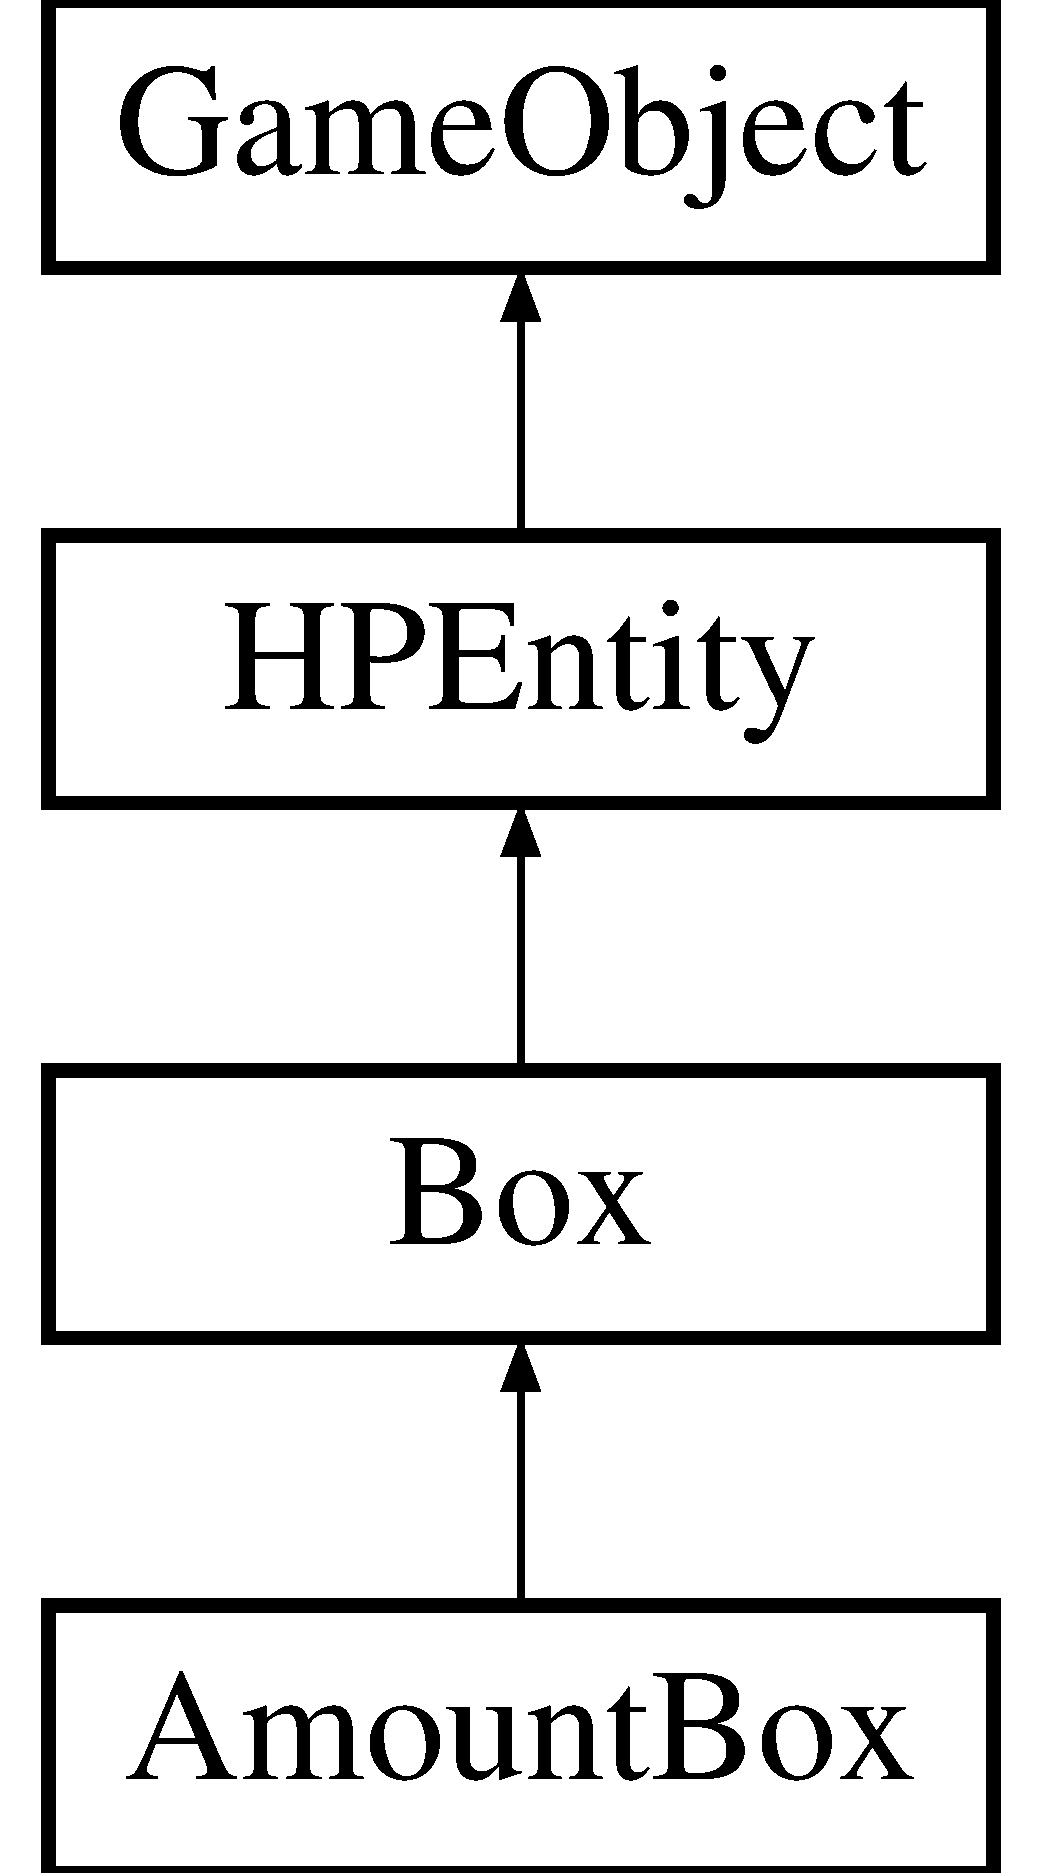
\includegraphics[height=4.000000cm]{class_amount_box}
\end{center}
\end{figure}
\subsection*{Public Member Functions}
\begin{DoxyCompactItemize}
\item 
\hyperlink{class_amount_box_a19f89bb62420a75212487fd191f256c4}{Amount\-Box} (Q\-Rect p\-Rect, int p\-Max\-Hp, int p\-Points\-To\-Add)
\begin{DoxyCompactList}\small\item\em Constructor de la clase, le da una posicion, una vida maxima que pueda soportar y la cantidad de disparos que le agrega al jugador que colisione con esta. \end{DoxyCompactList}\item 
void \hyperlink{class_amount_box_a006ae7739b2e6dbbb19c0a2a09936a71}{add\-Points\-To\-Player} (\hyperlink{class_player}{Player} $\ast$p\-Player)
\begin{DoxyCompactList}\small\item\em es el metodo que se encarga de agregar o quitar los puntos actuales de la caja sumara o dejara intacto la vida de este, dependiendo de los puntos que esta tenga \end{DoxyCompactList}\item 
virtual \hyperlink{class_amount_box_a4d6ec95818bed923b6c19e1df6b50db8}{$\sim$\-Amount\-Box} ()
\begin{DoxyCompactList}\small\item\em constructor virtual de la clase \end{DoxyCompactList}\end{DoxyCompactItemize}
\subsection*{Additional Inherited Members}


\subsection{Detailed Description}
Esta clase es la que se encarga de dar municiones al personaje, es la caja que aparece aleatoriamente sobre la ventana y da las municiones o disparos. 

\subsection{Constructor \& Destructor Documentation}
\hypertarget{class_amount_box_a19f89bb62420a75212487fd191f256c4}{\index{Amount\-Box@{Amount\-Box}!Amount\-Box@{Amount\-Box}}
\index{Amount\-Box@{Amount\-Box}!AmountBox@{Amount\-Box}}
\subsubsection[{Amount\-Box}]{\setlength{\rightskip}{0pt plus 5cm}Amount\-Box\-::\-Amount\-Box (
\begin{DoxyParamCaption}
\item[{Q\-Rect}]{p\-Rect, }
\item[{int}]{p\-Max\-Hp, }
\item[{int}]{p\-Points\-To\-Add}
\end{DoxyParamCaption}
)}}\label{class_amount_box_a19f89bb62420a75212487fd191f256c4}


Constructor de la clase, le da una posicion, una vida maxima que pueda soportar y la cantidad de disparos que le agrega al jugador que colisione con esta. 


\begin{DoxyParams}{Parameters}
{\em p\-Rect} & el rectangulo que contiene las dimensiones y la posicion del mismo \\
\hline
{\em p\-Max\-Hp} & es la vida maxima del la caja \\
\hline
{\em p\-Points\-To\-Add} & la cantidad de puntos agregara al jugador con el que colisione \\
\hline
\end{DoxyParams}
\hypertarget{class_amount_box_a4d6ec95818bed923b6c19e1df6b50db8}{\index{Amount\-Box@{Amount\-Box}!$\sim$\-Amount\-Box@{$\sim$\-Amount\-Box}}
\index{$\sim$\-Amount\-Box@{$\sim$\-Amount\-Box}!AmountBox@{Amount\-Box}}
\subsubsection[{$\sim$\-Amount\-Box}]{\setlength{\rightskip}{0pt plus 5cm}Amount\-Box\-::$\sim$\-Amount\-Box (
\begin{DoxyParamCaption}
{}
\end{DoxyParamCaption}
)\hspace{0.3cm}{\ttfamily [virtual]}}}\label{class_amount_box_a4d6ec95818bed923b6c19e1df6b50db8}


constructor virtual de la clase 



\subsection{Member Function Documentation}
\hypertarget{class_amount_box_a006ae7739b2e6dbbb19c0a2a09936a71}{\index{Amount\-Box@{Amount\-Box}!add\-Points\-To\-Player@{add\-Points\-To\-Player}}
\index{add\-Points\-To\-Player@{add\-Points\-To\-Player}!AmountBox@{Amount\-Box}}
\subsubsection[{add\-Points\-To\-Player}]{\setlength{\rightskip}{0pt plus 5cm}void Amount\-Box\-::add\-Points\-To\-Player (
\begin{DoxyParamCaption}
\item[{{\bf Player} $\ast$}]{p\-Player}
\end{DoxyParamCaption}
)\hspace{0.3cm}{\ttfamily [virtual]}}}\label{class_amount_box_a006ae7739b2e6dbbb19c0a2a09936a71}


es el metodo que se encarga de agregar o quitar los puntos actuales de la caja sumara o dejara intacto la vida de este, dependiendo de los puntos que esta tenga 


\begin{DoxyParams}{Parameters}
{\em p\-Player} & es el jugador al cual se le sumaran o sustraera las municiones \\
\hline
\end{DoxyParams}


Reimplemented from \hyperlink{class_box_a536c605982fc2000fbda0388d0a2fb2b}{Box}.



The documentation for this class was generated from the following files\-:\begin{DoxyCompactItemize}
\item 
logic/mapobjects/\hyperlink{amountbox_8h}{amountbox.\-h}\item 
logic/mapobjects/\hyperlink{amountbox_8cpp}{amountbox.\-cpp}\end{DoxyCompactItemize}

\hypertarget{class_angle_shot}{\section{Angle\-Shot Class Reference}
\label{class_angle_shot}\index{Angle\-Shot@{Angle\-Shot}}
}


{\ttfamily \#include $<$angleshot.\-h$>$}

Inheritance diagram for Angle\-Shot\-:\begin{figure}[H]
\begin{center}
\leavevmode
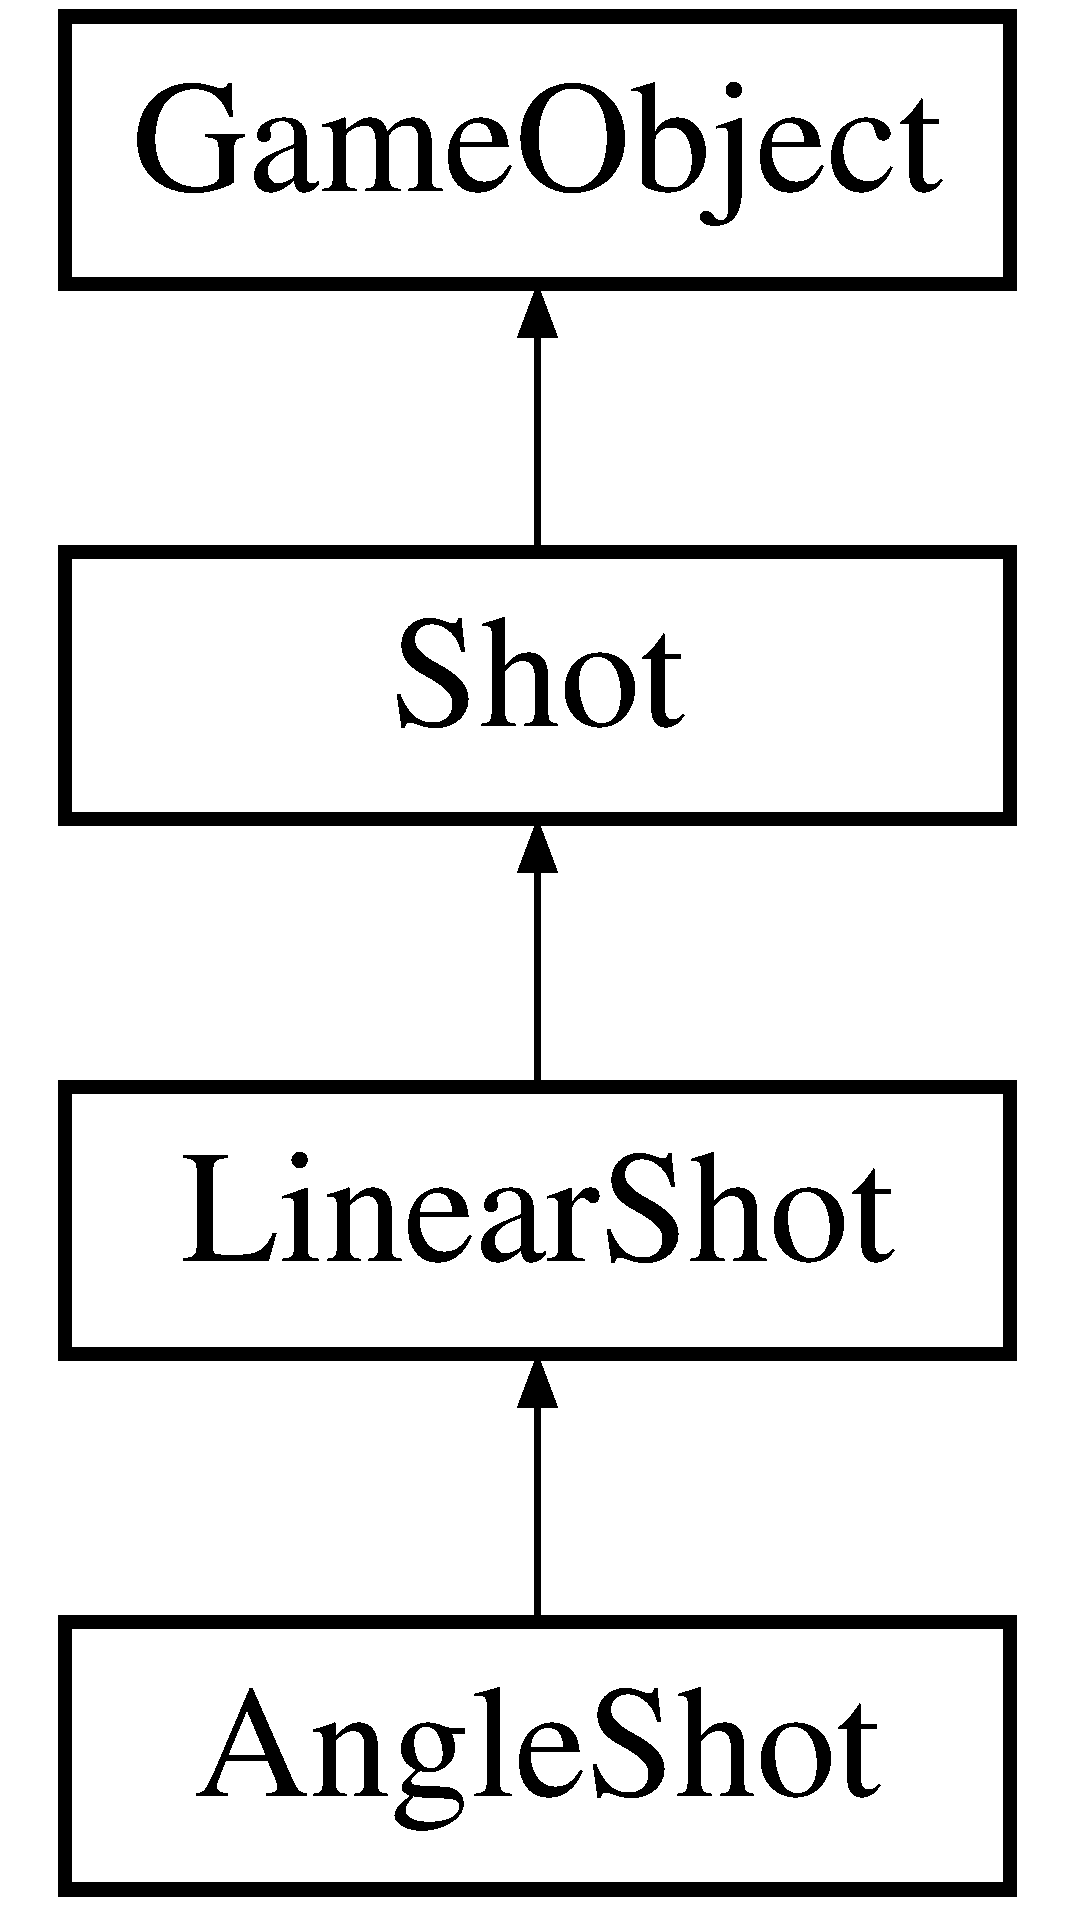
\includegraphics[height=4.000000cm]{class_angle_shot}
\end{center}
\end{figure}
\subsection*{Public Member Functions}
\begin{DoxyCompactItemize}
\item 
\hyperlink{class_angle_shot_ae25e86a55ee3c18b1c8be4731729059d}{Angle\-Shot} (Q\-Rect p\-Rectangle, int p\-Damage, float p\-Angle)
\item 
void \hyperlink{class_angle_shot_a15e9f45aedf1a47836b0c603a758dd20}{update} ()
\begin{DoxyCompactList}\small\item\em Actualiza el objeto, es un metodo abstracto, y debe ser implementado por sus clases hijas. \end{DoxyCompactList}\item 
int \hyperlink{class_angle_shot_a690154e0ae49ac8667046f0c4a9c1647}{get\-Type} ()
\item 
int \hyperlink{class_angle_shot_a7e51f41031536ff1086055eab24d544d}{get\-X\-Velocity} ()
\item 
virtual \hyperlink{class_angle_shot_af12cb94bb36cfcfd02108d0f74d2655c}{$\sim$\-Angle\-Shot} ()
\end{DoxyCompactItemize}
\subsection*{Additional Inherited Members}


\subsection{Constructor \& Destructor Documentation}
\hypertarget{class_angle_shot_ae25e86a55ee3c18b1c8be4731729059d}{\index{Angle\-Shot@{Angle\-Shot}!Angle\-Shot@{Angle\-Shot}}
\index{Angle\-Shot@{Angle\-Shot}!AngleShot@{Angle\-Shot}}
\subsubsection[{Angle\-Shot}]{\setlength{\rightskip}{0pt plus 5cm}Angle\-Shot\-::\-Angle\-Shot (
\begin{DoxyParamCaption}
\item[{Q\-Rect}]{p\-Rectangle, }
\item[{int}]{p\-Damage, }
\item[{float}]{p\-Angle}
\end{DoxyParamCaption}
)}}\label{class_angle_shot_ae25e86a55ee3c18b1c8be4731729059d}
\hypertarget{class_angle_shot_af12cb94bb36cfcfd02108d0f74d2655c}{\index{Angle\-Shot@{Angle\-Shot}!$\sim$\-Angle\-Shot@{$\sim$\-Angle\-Shot}}
\index{$\sim$\-Angle\-Shot@{$\sim$\-Angle\-Shot}!AngleShot@{Angle\-Shot}}
\subsubsection[{$\sim$\-Angle\-Shot}]{\setlength{\rightskip}{0pt plus 5cm}Angle\-Shot\-::$\sim$\-Angle\-Shot (
\begin{DoxyParamCaption}
{}
\end{DoxyParamCaption}
)\hspace{0.3cm}{\ttfamily [virtual]}}}\label{class_angle_shot_af12cb94bb36cfcfd02108d0f74d2655c}


\subsection{Member Function Documentation}
\hypertarget{class_angle_shot_a690154e0ae49ac8667046f0c4a9c1647}{\index{Angle\-Shot@{Angle\-Shot}!get\-Type@{get\-Type}}
\index{get\-Type@{get\-Type}!AngleShot@{Angle\-Shot}}
\subsubsection[{get\-Type}]{\setlength{\rightskip}{0pt plus 5cm}int Angle\-Shot\-::get\-Type (
\begin{DoxyParamCaption}
{}
\end{DoxyParamCaption}
)\hspace{0.3cm}{\ttfamily [virtual]}}}\label{class_angle_shot_a690154e0ae49ac8667046f0c4a9c1647}


Implements \hyperlink{class_shot_a3bf2af64550a0ee1d467bdec43ac6200}{Shot}.

\hypertarget{class_angle_shot_a7e51f41031536ff1086055eab24d544d}{\index{Angle\-Shot@{Angle\-Shot}!get\-X\-Velocity@{get\-X\-Velocity}}
\index{get\-X\-Velocity@{get\-X\-Velocity}!AngleShot@{Angle\-Shot}}
\subsubsection[{get\-X\-Velocity}]{\setlength{\rightskip}{0pt plus 5cm}int Angle\-Shot\-::get\-X\-Velocity (
\begin{DoxyParamCaption}
{}
\end{DoxyParamCaption}
)\hspace{0.3cm}{\ttfamily [virtual]}}}\label{class_angle_shot_a7e51f41031536ff1086055eab24d544d}


Implements \hyperlink{class_shot_a8cfb5cf554b6164f2dceef2e7263b8a0}{Shot}.

\hypertarget{class_angle_shot_a15e9f45aedf1a47836b0c603a758dd20}{\index{Angle\-Shot@{Angle\-Shot}!update@{update}}
\index{update@{update}!AngleShot@{Angle\-Shot}}
\subsubsection[{update}]{\setlength{\rightskip}{0pt plus 5cm}void Angle\-Shot\-::update (
\begin{DoxyParamCaption}
{}
\end{DoxyParamCaption}
)\hspace{0.3cm}{\ttfamily [virtual]}}}\label{class_angle_shot_a15e9f45aedf1a47836b0c603a758dd20}


Actualiza el objeto, es un metodo abstracto, y debe ser implementado por sus clases hijas. 



Implements \hyperlink{class_game_object_ae83128d0e0efef691417779605ee037c}{Game\-Object}.



The documentation for this class was generated from the following files\-:\begin{DoxyCompactItemize}
\item 
logic/shot/\hyperlink{angleshot_8h}{angleshot.\-h}\item 
logic/shot/\hyperlink{angleshot_8cpp}{angleshot.\-cpp}\end{DoxyCompactItemize}

\hypertarget{class_angle_shot_manager}{\section{Angle\-Shot\-Manager Class Reference}
\label{class_angle_shot_manager}\index{Angle\-Shot\-Manager@{Angle\-Shot\-Manager}}
}
Inheritance diagram for Angle\-Shot\-Manager\-:\begin{figure}[H]
\begin{center}
\leavevmode
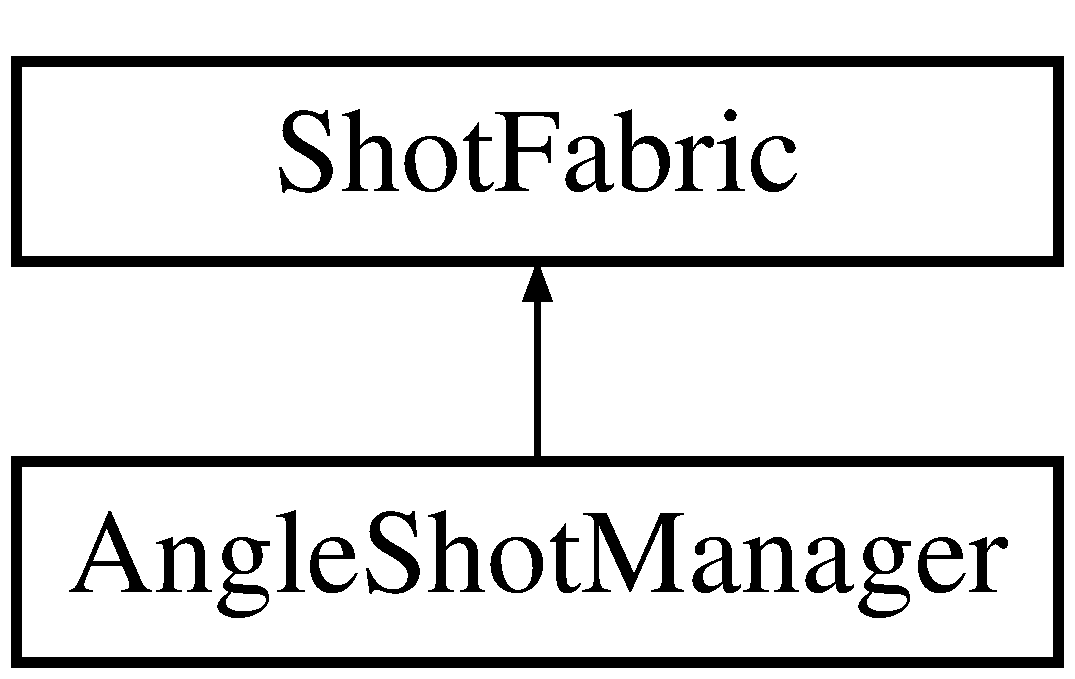
\includegraphics[height=2.000000cm]{class_angle_shot_manager}
\end{center}
\end{figure}
\subsection*{Public Member Functions}
\begin{DoxyCompactItemize}
\item 
\hypertarget{class_angle_shot_manager_a54c7a8671c85d42273c716a66a699824}{{\bfseries Angle\-Shot\-Manager} (int p\-Max\-Munition)}\label{class_angle_shot_manager_a54c7a8671c85d42273c716a66a699824}

\item 
\hypertarget{class_angle_shot_manager_ab572dadf520c29aca5f563f88cc8655d}{\hyperlink{class_shot}{Shot} $\ast$ {\bfseries get\-New\-Shoot} (int p\-X, int p\-Y, bool p\-Player)}\label{class_angle_shot_manager_ab572dadf520c29aca5f563f88cc8655d}

\item 
\hypertarget{class_angle_shot_manager_ab7a210ac59c662552496f301d52a3ec0}{int {\bfseries get\-Munition\-Type} ()}\label{class_angle_shot_manager_ab7a210ac59c662552496f301d52a3ec0}

\end{DoxyCompactItemize}
\subsection*{Additional Inherited Members}


The documentation for this class was generated from the following files\-:\begin{DoxyCompactItemize}
\item 
logic/shot/angleshotmanager.\-h\item 
logic/shot/angleshotmanager.\-cpp\end{DoxyCompactItemize}

\hypertarget{class_box}{\section{Box Class Reference}
\label{class_box}\index{Box@{Box}}
}


Es la clase caja que se encarga de agregar puntos de vida al jugador, tambien se encarga de quitarle puntos si se ha convertido en una caja envenenada.  




{\ttfamily \#include $<$box.\-h$>$}

Inheritance diagram for Box\-:\begin{figure}[H]
\begin{center}
\leavevmode
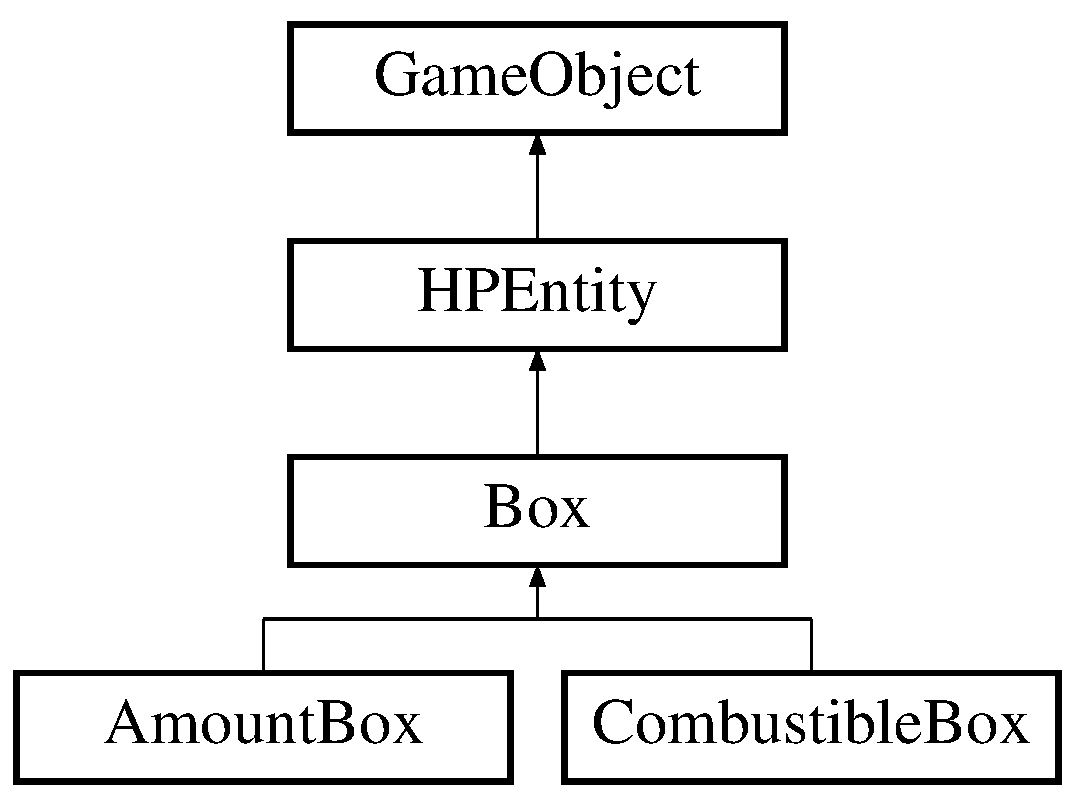
\includegraphics[height=4.000000cm]{class_box}
\end{center}
\end{figure}
\subsection*{Public Member Functions}
\begin{DoxyCompactItemize}
\item 
\hyperlink{class_box_a12c7c3f710d76e599a31e7a41784f613}{Box} (Q\-Rect p\-Rect, int p\-Max\-Hp, int p\-Points\-To\-Add)
\begin{DoxyCompactList}\small\item\em Es el constructor de la clase box le da una posicion (x,y) y dimensiones, una cantidad de vida maxima y la cantidad de puntos que agregara. \end{DoxyCompactList}\item 
virtual void \hyperlink{class_box_a536c605982fc2000fbda0388d0a2fb2b}{add\-Points\-To\-Player} (\hyperlink{class_player}{Player} $\ast$p\-Player)
\begin{DoxyCompactList}\small\item\em Es el metodo que se encarga de sumar o restar directamente la vida al jugador. \end{DoxyCompactList}\item 
void \hyperlink{class_box_a82b510b4e487f29189b19699ebaaebae}{turn\-Abad\-Box} ()
\begin{DoxyCompactList}\small\item\em Este metodo se encarga de tornar la caja en una caja mala volviedo los puntos que esta contiene en puntos negativos que afectaran directamente sobre el jugador. \end{DoxyCompactList}\item 
bool \hyperlink{class_box_a1d84b0a091465889a6e587c4f9072482}{is\-Bad\-Box} ()
\begin{DoxyCompactList}\small\item\em Verifica si la caja es mala, osea perjudica al jugador. \end{DoxyCompactList}\item 
void \hyperlink{class_box_a779104150a6f06da2bf1500489a58530}{update} ()
\begin{DoxyCompactList}\small\item\em Actualiza las posiciones y puntos de la caja. \end{DoxyCompactList}\item 
virtual \hyperlink{class_box_a6a5e09398e85d602a046b429062fb9c2}{$\sim$\-Box} ()
\begin{DoxyCompactList}\small\item\em Destructor virtual de la clase. \end{DoxyCompactList}\end{DoxyCompactItemize}
\subsection*{Protected Attributes}
\begin{DoxyCompactItemize}
\item 
int \hyperlink{class_box_a6bad20b31366e6c10dd372d46521f566}{\-\_\-\-Points\-To\-Add}
\end{DoxyCompactItemize}
\subsection*{Additional Inherited Members}


\subsection{Detailed Description}
Es la clase caja que se encarga de agregar puntos de vida al jugador, tambien se encarga de quitarle puntos si se ha convertido en una caja envenenada. 

\subsection{Constructor \& Destructor Documentation}
\hypertarget{class_box_a12c7c3f710d76e599a31e7a41784f613}{\index{Box@{Box}!Box@{Box}}
\index{Box@{Box}!Box@{Box}}
\subsubsection[{Box}]{\setlength{\rightskip}{0pt plus 5cm}Box\-::\-Box (
\begin{DoxyParamCaption}
\item[{Q\-Rect}]{p\-Rect, }
\item[{int}]{p\-Max\-Hp, }
\item[{int}]{p\-Points\-To\-Add}
\end{DoxyParamCaption}
)}}\label{class_box_a12c7c3f710d76e599a31e7a41784f613}


Es el constructor de la clase box le da una posicion (x,y) y dimensiones, una cantidad de vida maxima y la cantidad de puntos que agregara. 


\begin{DoxyParams}{Parameters}
{\em p\-Rect} & Es el rectangulo que contiene la posicion y las dimensiones de la caja \\
\hline
{\em p\-Max\-Hp} & es la cantidad de vida maxima que esta contiene \\
\hline
{\em p\-Points\-To\-Add} & es la cantidad de vida que se agregara o sustreara del jugador \\
\hline
\end{DoxyParams}
\hypertarget{class_box_a6a5e09398e85d602a046b429062fb9c2}{\index{Box@{Box}!$\sim$\-Box@{$\sim$\-Box}}
\index{$\sim$\-Box@{$\sim$\-Box}!Box@{Box}}
\subsubsection[{$\sim$\-Box}]{\setlength{\rightskip}{0pt plus 5cm}Box\-::$\sim$\-Box (
\begin{DoxyParamCaption}
{}
\end{DoxyParamCaption}
)\hspace{0.3cm}{\ttfamily [virtual]}}}\label{class_box_a6a5e09398e85d602a046b429062fb9c2}


Destructor virtual de la clase. 



\subsection{Member Function Documentation}
\hypertarget{class_box_a536c605982fc2000fbda0388d0a2fb2b}{\index{Box@{Box}!add\-Points\-To\-Player@{add\-Points\-To\-Player}}
\index{add\-Points\-To\-Player@{add\-Points\-To\-Player}!Box@{Box}}
\subsubsection[{add\-Points\-To\-Player}]{\setlength{\rightskip}{0pt plus 5cm}void Box\-::add\-Points\-To\-Player (
\begin{DoxyParamCaption}
\item[{{\bf Player} $\ast$}]{p\-Player}
\end{DoxyParamCaption}
)\hspace{0.3cm}{\ttfamily [virtual]}}}\label{class_box_a536c605982fc2000fbda0388d0a2fb2b}


Es el metodo que se encarga de sumar o restar directamente la vida al jugador. 


\begin{DoxyParams}{Parameters}
{\em p\-Player} & es el jugador al que se le aplica la operacion de suma o resta de vida \\
\hline
\end{DoxyParams}


Reimplemented in \hyperlink{class_amount_box_a006ae7739b2e6dbbb19c0a2a09936a71}{Amount\-Box}, and \hyperlink{class_combustible_box_abab14feb7a19ee2a9fc61bbb1a92726a}{Combustible\-Box}.

\hypertarget{class_box_a1d84b0a091465889a6e587c4f9072482}{\index{Box@{Box}!is\-Bad\-Box@{is\-Bad\-Box}}
\index{is\-Bad\-Box@{is\-Bad\-Box}!Box@{Box}}
\subsubsection[{is\-Bad\-Box}]{\setlength{\rightskip}{0pt plus 5cm}bool Box\-::is\-Bad\-Box (
\begin{DoxyParamCaption}
{}
\end{DoxyParamCaption}
)}}\label{class_box_a1d84b0a091465889a6e587c4f9072482}


Verifica si la caja es mala, osea perjudica al jugador. 

\begin{DoxyReturn}{Returns}
true, si la caja es mala 
\end{DoxyReturn}
\hypertarget{class_box_a82b510b4e487f29189b19699ebaaebae}{\index{Box@{Box}!turn\-Abad\-Box@{turn\-Abad\-Box}}
\index{turn\-Abad\-Box@{turn\-Abad\-Box}!Box@{Box}}
\subsubsection[{turn\-Abad\-Box}]{\setlength{\rightskip}{0pt plus 5cm}void Box\-::turn\-Abad\-Box (
\begin{DoxyParamCaption}
{}
\end{DoxyParamCaption}
)}}\label{class_box_a82b510b4e487f29189b19699ebaaebae}


Este metodo se encarga de tornar la caja en una caja mala volviedo los puntos que esta contiene en puntos negativos que afectaran directamente sobre el jugador. 

\hypertarget{class_box_a779104150a6f06da2bf1500489a58530}{\index{Box@{Box}!update@{update}}
\index{update@{update}!Box@{Box}}
\subsubsection[{update}]{\setlength{\rightskip}{0pt plus 5cm}void Box\-::update (
\begin{DoxyParamCaption}
{}
\end{DoxyParamCaption}
)\hspace{0.3cm}{\ttfamily [virtual]}}}\label{class_box_a779104150a6f06da2bf1500489a58530}


Actualiza las posiciones y puntos de la caja. 



Implements \hyperlink{class_game_object_ae83128d0e0efef691417779605ee037c}{Game\-Object}.



Reimplemented in \hyperlink{class_combustible_box_ac3bcbb721576f4b00b0f2d7e48994657}{Combustible\-Box}.



\subsection{Member Data Documentation}
\hypertarget{class_box_a6bad20b31366e6c10dd372d46521f566}{\index{Box@{Box}!\-\_\-\-Points\-To\-Add@{\-\_\-\-Points\-To\-Add}}
\index{\-\_\-\-Points\-To\-Add@{\-\_\-\-Points\-To\-Add}!Box@{Box}}
\subsubsection[{\-\_\-\-Points\-To\-Add}]{\setlength{\rightskip}{0pt plus 5cm}int Box\-::\-\_\-\-Points\-To\-Add\hspace{0.3cm}{\ttfamily [protected]}}}\label{class_box_a6bad20b31366e6c10dd372d46521f566}
T\-O\-D\-O son los puntos que agregara 

The documentation for this class was generated from the following files\-:\begin{DoxyCompactItemize}
\item 
logic/mapobjects/\hyperlink{box_8h}{box.\-h}\item 
logic/mapobjects/\hyperlink{box_8cpp}{box.\-cpp}\end{DoxyCompactItemize}

\hypertarget{class_bridge}{\section{Bridge Class Reference}
\label{class_bridge}\index{Bridge@{Bridge}}
}


The documentation for this class was generated from the following files\-:\begin{DoxyCompactItemize}
\item 
logic/mapobjects/bridge.\-h\item 
logic/mapobjects/bridge.\-cpp\end{DoxyCompactItemize}

\hypertarget{class_change_phase}{\section{Change\-Phase Class Reference}
\label{class_change_phase}\index{Change\-Phase@{Change\-Phase}}
}
Inheritance diagram for Change\-Phase\-:\begin{figure}[H]
\begin{center}
\leavevmode
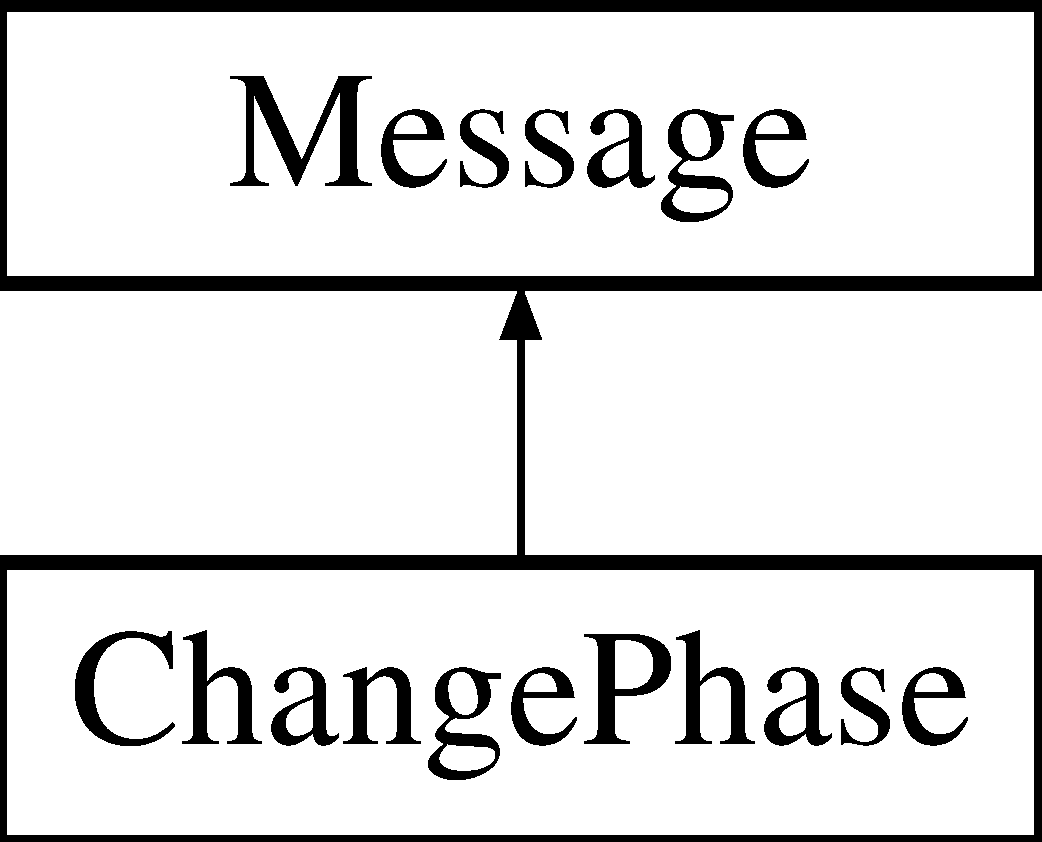
\includegraphics[height=2.000000cm]{class_change_phase}
\end{center}
\end{figure}
\subsection*{Public Member Functions}
\begin{DoxyCompactItemize}
\item 
\hypertarget{class_change_phase_a4b9f1307f5e414f9e31028593df82821}{{\bfseries Change\-Phase} (const \hyperlink{class_change_phase}{Change\-Phase} \&from)}\label{class_change_phase_a4b9f1307f5e414f9e31028593df82821}

\item 
\hypertarget{class_change_phase_afe1b8fb71c597241a130e5a0361084ff}{\hyperlink{class_change_phase}{Change\-Phase} \& {\bfseries operator=} (const \hyperlink{class_change_phase}{Change\-Phase} \&from)}\label{class_change_phase_afe1b8fb71c597241a130e5a0361084ff}

\item 
\hypertarget{class_change_phase_a35fed0c7a4fe24a8aa7fdeedde702f25}{const \\*
\-::google\-::protobuf\-::\-Unknown\-Field\-Set \& {\bfseries unknown\-\_\-fields} () const }\label{class_change_phase_a35fed0c7a4fe24a8aa7fdeedde702f25}

\item 
\hypertarget{class_change_phase_ae7bdf30321b4858a0947396ed19a8d9c}{inline\-::google\-::protobuf\-::\-Unknown\-Field\-Set $\ast$ {\bfseries mutable\-\_\-unknown\-\_\-fields} ()}\label{class_change_phase_ae7bdf30321b4858a0947396ed19a8d9c}

\item 
\hypertarget{class_change_phase_a4be33194d239e28dd0aecaf4d836a809}{void {\bfseries Swap} (\hyperlink{class_change_phase}{Change\-Phase} $\ast$other)}\label{class_change_phase_a4be33194d239e28dd0aecaf4d836a809}

\item 
\hypertarget{class_change_phase_a9c62cc118ada96ab07093b542f54f651}{\hyperlink{class_change_phase}{Change\-Phase} $\ast$ {\bfseries New} () const }\label{class_change_phase_a9c62cc118ada96ab07093b542f54f651}

\item 
\hypertarget{class_change_phase_af8041c1ea9d514c054ff97dea9691413}{\hyperlink{class_change_phase}{Change\-Phase} $\ast$ {\bfseries New} (\-::google\-::protobuf\-::\-Arena $\ast$arena) const }\label{class_change_phase_af8041c1ea9d514c054ff97dea9691413}

\item 
\hypertarget{class_change_phase_aaa00056e07d103185fb7d3c9b2c80c89}{void {\bfseries Copy\-From} (const \-::google\-::protobuf\-::\-Message \&from)}\label{class_change_phase_aaa00056e07d103185fb7d3c9b2c80c89}

\item 
\hypertarget{class_change_phase_a0b4ea2d69bef41bfd5def289ed42f48b}{void {\bfseries Merge\-From} (const \-::google\-::protobuf\-::\-Message \&from)}\label{class_change_phase_a0b4ea2d69bef41bfd5def289ed42f48b}

\item 
\hypertarget{class_change_phase_acc54fcc2735378a34fe9f313b0d28d90}{void {\bfseries Copy\-From} (const \hyperlink{class_change_phase}{Change\-Phase} \&from)}\label{class_change_phase_acc54fcc2735378a34fe9f313b0d28d90}

\item 
\hypertarget{class_change_phase_a980a96f372dbf4eeff624c0ae7cb8537}{void {\bfseries Merge\-From} (const \hyperlink{class_change_phase}{Change\-Phase} \&from)}\label{class_change_phase_a980a96f372dbf4eeff624c0ae7cb8537}

\item 
\hypertarget{class_change_phase_ae5f1923ed41767cee32ef3475ad75ce0}{void {\bfseries Clear} ()}\label{class_change_phase_ae5f1923ed41767cee32ef3475ad75ce0}

\item 
\hypertarget{class_change_phase_a2fa641d0ce528ee22615eae08c8193cc}{bool {\bfseries Is\-Initialized} () const }\label{class_change_phase_a2fa641d0ce528ee22615eae08c8193cc}

\item 
\hypertarget{class_change_phase_adb5d0c836b47a428c7b8a8b11cc889e0}{int {\bfseries Byte\-Size} () const }\label{class_change_phase_adb5d0c836b47a428c7b8a8b11cc889e0}

\item 
\hypertarget{class_change_phase_a5cf5896de3c53cf0430b6747539fbb48}{bool {\bfseries Merge\-Partial\-From\-Coded\-Stream} (\-::google\-::protobuf\-::io\-::\-Coded\-Input\-Stream $\ast$input)}\label{class_change_phase_a5cf5896de3c53cf0430b6747539fbb48}

\item 
\hypertarget{class_change_phase_aa35438674277382e3a4e5c23d477cde6}{void {\bfseries Serialize\-With\-Cached\-Sizes} (\-::google\-::protobuf\-::io\-::\-Coded\-Output\-Stream $\ast$output) const }\label{class_change_phase_aa35438674277382e3a4e5c23d477cde6}

\item 
\hypertarget{class_change_phase_aa7987128eb875e6387cddb886094b922}{\-::google\-::protobuf\-::uint8 $\ast$ {\bfseries Serialize\-With\-Cached\-Sizes\-To\-Array} (\-::google\-::protobuf\-::uint8 $\ast$output) const }\label{class_change_phase_aa7987128eb875e6387cddb886094b922}

\item 
\hypertarget{class_change_phase_a061c6426b4e079d7fe6ade662e3fcb60}{int {\bfseries Get\-Cached\-Size} () const }\label{class_change_phase_a061c6426b4e079d7fe6ade662e3fcb60}

\item 
\hypertarget{class_change_phase_adf1e1f91fda84e9fcbc64a32d0442ee8}{\-::google\-::protobuf\-::\-Metadata {\bfseries Get\-Metadata} () const }\label{class_change_phase_adf1e1f91fda84e9fcbc64a32d0442ee8}

\item 
\hypertarget{class_change_phase_aebfe231080875edab422c1332fb9848c}{bool {\bfseries has\-\_\-numofphase} () const }\label{class_change_phase_aebfe231080875edab422c1332fb9848c}

\item 
\hypertarget{class_change_phase_ad0d17253d8988af5afa6f3b81235164e}{void {\bfseries clear\-\_\-numofphase} ()}\label{class_change_phase_ad0d17253d8988af5afa6f3b81235164e}

\item 
\hypertarget{class_change_phase_a00b30bc0d542ab389b7b20aaae1b10bc}{inline\-::google\-::protobuf\-::int32 {\bfseries numofphase} () const }\label{class_change_phase_a00b30bc0d542ab389b7b20aaae1b10bc}

\item 
\hypertarget{class_change_phase_a40d66346dfc6aae8de80fb5545fe8460}{void {\bfseries set\-\_\-numofphase} (\-::google\-::protobuf\-::int32 value)}\label{class_change_phase_a40d66346dfc6aae8de80fb5545fe8460}

\end{DoxyCompactItemize}
\subsection*{Static Public Member Functions}
\begin{DoxyCompactItemize}
\item 
\hypertarget{class_change_phase_abc14333ee6f01fd88840e430c202f926}{static const \\*
\-::google\-::protobuf\-::\-Descriptor $\ast$ {\bfseries descriptor} ()}\label{class_change_phase_abc14333ee6f01fd88840e430c202f926}

\item 
\hypertarget{class_change_phase_a2a86feb8760cbad6c536e5f836ba6755}{static const \hyperlink{class_change_phase}{Change\-Phase} \& {\bfseries default\-\_\-instance} ()}\label{class_change_phase_a2a86feb8760cbad6c536e5f836ba6755}

\end{DoxyCompactItemize}
\subsection*{Static Public Attributes}
\begin{DoxyCompactItemize}
\item 
\hypertarget{class_change_phase_a19b42121df5751cc03a51d1244186f6b}{static const int {\bfseries k\-Num\-Of\-Phase\-Field\-Number} = 1}\label{class_change_phase_a19b42121df5751cc03a51d1244186f6b}

\end{DoxyCompactItemize}
\subsection*{Friends}
\begin{DoxyCompactItemize}
\item 
\hypertarget{class_change_phase_a4647c51e7b88278f5694cd14cbc5e191}{void {\bfseries protobuf\-\_\-\-Add\-Desc\-\_\-\-Change\-Phase\-\_\-2eproto} ()}\label{class_change_phase_a4647c51e7b88278f5694cd14cbc5e191}

\item 
\hypertarget{class_change_phase_a1fdbab9f17b7cba7ac51b7d21e9a0700}{void {\bfseries protobuf\-\_\-\-Assign\-Desc\-\_\-\-Change\-Phase\-\_\-2eproto} ()}\label{class_change_phase_a1fdbab9f17b7cba7ac51b7d21e9a0700}

\item 
\hypertarget{class_change_phase_a20ac3c1c2ccf4bf4b4a4f0841d1258f7}{void {\bfseries protobuf\-\_\-\-Shutdown\-File\-\_\-\-Change\-Phase\-\_\-2eproto} ()}\label{class_change_phase_a20ac3c1c2ccf4bf4b4a4f0841d1258f7}

\end{DoxyCompactItemize}


The documentation for this class was generated from the following files\-:\begin{DoxyCompactItemize}
\item 
protobufmessage/Change\-Phase.\-pb.\-h\item 
protobufmessage/Change\-Phase.\-pb.\-cc\end{DoxyCompactItemize}

\hypertarget{class_circular_list}{\section{Circular\-List$<$ E $>$ Class Template Reference}
\label{class_circular_list}\index{Circular\-List$<$ E $>$@{Circular\-List$<$ E $>$}}
}


Esta clase es una estructura de datos especificamente una lista enlazada circular simple que puede contener cualquier tipo de dato solamente definiciendolo mediante el template de esta clase. se puede agregar y borrar el dato.  




{\ttfamily \#include $<$Circular\-List.\-h$>$}

Inheritance diagram for Circular\-List$<$ E $>$\-:\begin{figure}[H]
\begin{center}
\leavevmode
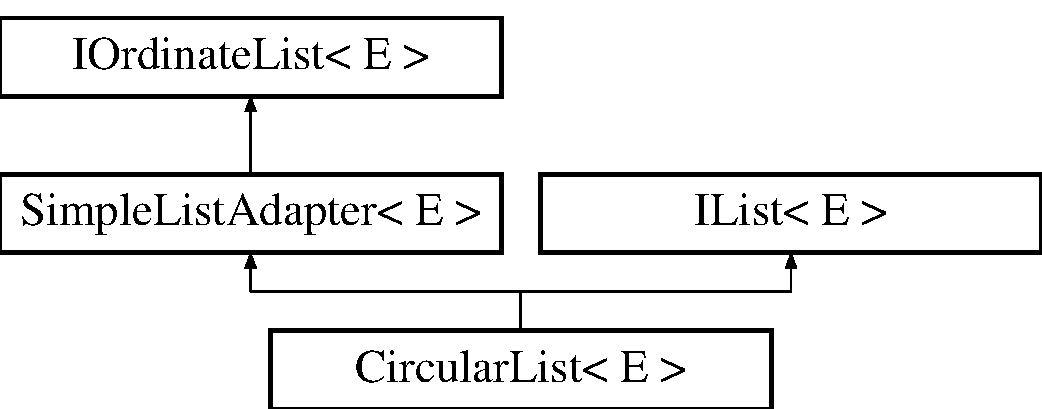
\includegraphics[height=3.000000cm]{class_circular_list}
\end{center}
\end{figure}
\subsection*{Public Member Functions}
\begin{DoxyCompactItemize}
\item 
\hypertarget{class_circular_list_aad23571a808ede6fc0432dca645ab2ca}{\hyperlink{class_circular_list_aad23571a808ede6fc0432dca645ab2ca}{Circular\-List} ()}\label{class_circular_list_aad23571a808ede6fc0432dca645ab2ca}

\begin{DoxyCompactList}\small\item\em Es el constructor de la lista circular simple. \end{DoxyCompactList}\item 
void \hyperlink{class_circular_list_a275c75e142e791de9a1a00691af56a73}{addi} (E)
\begin{DoxyCompactList}\small\item\em Agrega un elemento al principio de la lista. \end{DoxyCompactList}\item 
void \hyperlink{class_circular_list_a892b493309f36fb083fdd257388cfa36}{add} (E)
\begin{DoxyCompactList}\small\item\em Agregar un elemento al final de la lista. \end{DoxyCompactList}\item 
bool \hyperlink{class_circular_list_af184d3ac2e3bba683a44a6cc19392b12}{add} (E, int)
\begin{DoxyCompactList}\small\item\em Agrega el elemento en el indice indicado. Si el indice es incorrecto no se agrega el elemento. \end{DoxyCompactList}\item 
bool \hyperlink{class_circular_list_a4a6acfd818a0ae9055957ec80258c60a}{remove} (int)
\begin{DoxyCompactList}\small\item\em Remueve el dato en la posicion indicada por el parametro, en caso que el indice indicado sea incorrecto, osea que sea menor que cero o mayor o igual que el largo de la lista no alterara la lista. \end{DoxyCompactList}\item 
void \hyperlink{class_circular_list_aa54489e11ad76bf929f92b1dce97a3a3}{set} (int, E)
\begin{DoxyCompactList}\small\item\em Setea el valor del dato que se encuentre en el indice citado con un nuevo valor. \end{DoxyCompactList}\item 
E \hyperlink{class_circular_list_ad6783339c7ff05841fc62f74f809644d}{get} (int)
\begin{DoxyCompactList}\small\item\em Obtiene un dato el la posicion indicada. En caso que el indice indicado sea incorrecto, osea que sea menor que cero o mayor o igual que el largo de la lista arrojara un error pues el dato esta fuera de los limites de la lista. \end{DoxyCompactList}\item 
\hyperlink{class_i_iterator}{I\-Iterator}$<$ E $>$ $\ast$ \hyperlink{class_circular_list_a43e6cf1632001b3f409c6ce531529c6e}{get\-Iterator} ()
\begin{DoxyCompactList}\small\item\em Obtiene una instancia de un nuevo iterador de esta lista, y pueden obtenerse cuantas sean necesarias. pero es responsabilidad del programador eliminar mediante la palabra reservada delete. \end{DoxyCompactList}\item 
\hypertarget{class_circular_list_aa65c9665b7d36a5e609752cad0a35dbb}{virtual \hyperlink{class_circular_list_aa65c9665b7d36a5e609752cad0a35dbb}{$\sim$\-Circular\-List} ()}\label{class_circular_list_aa65c9665b7d36a5e609752cad0a35dbb}

\begin{DoxyCompactList}\small\item\em Es el destructor de la lista. \end{DoxyCompactList}\end{DoxyCompactItemize}
\subsection*{Protected Member Functions}
\begin{DoxyCompactItemize}
\item 
bool \hyperlink{class_circular_list_a6f405f4be7946286a958e0b83937b3e2}{addi} (E p\-Data)
\begin{DoxyCompactList}\small\item\em Agrega un elemento al principio de la lista. \end{DoxyCompactList}\item 
\hypertarget{class_circular_list_ad2832eb48d7d69fa5d759c0c16c4bc5e}{bool {\bfseries addf} (E p\-Data)}\label{class_circular_list_ad2832eb48d7d69fa5d759c0c16c4bc5e}

\item 
\hypertarget{class_circular_list_a0a3f318454d748eff1e3b8729aea94bd}{bool {\bfseries add\-First\-Data} (E p\-Data)}\label{class_circular_list_a0a3f318454d748eff1e3b8729aea94bd}

\item 
\hypertarget{class_circular_list_a706dd0ab6fb475bec90d9c40cefa92b1}{bool {\bfseries removei} ()}\label{class_circular_list_a706dd0ab6fb475bec90d9c40cefa92b1}

\item 
\hypertarget{class_circular_list_a1dde06b77306b31eb38fa4b43b6009ab}{bool {\bfseries removef} ()}\label{class_circular_list_a1dde06b77306b31eb38fa4b43b6009ab}

\end{DoxyCompactItemize}
\subsection*{Additional Inherited Members}


\subsection{Detailed Description}
\subsubsection*{template$<$class E$>$class Circular\-List$<$ E $>$}

Esta clase es una estructura de datos especificamente una lista enlazada circular simple que puede contener cualquier tipo de dato solamente definiciendolo mediante el template de esta clase. se puede agregar y borrar el dato. 

\subsection{Member Function Documentation}
\hypertarget{class_circular_list_a892b493309f36fb083fdd257388cfa36}{\index{Circular\-List@{Circular\-List}!add@{add}}
\index{add@{add}!CircularList@{Circular\-List}}
\subsubsection[{add}]{\setlength{\rightskip}{0pt plus 5cm}template$<$class E$>$ void {\bf Circular\-List}$<$ E $>$\-::add (
\begin{DoxyParamCaption}
\item[{E}]{data}
\end{DoxyParamCaption}
)\hspace{0.3cm}{\ttfamily [virtual]}}}\label{class_circular_list_a892b493309f36fb083fdd257388cfa36}


Agregar un elemento al final de la lista. 


\begin{DoxyParams}{Parameters}
{\em data} & el elemento a agregar \\
\hline
\end{DoxyParams}


Implements \hyperlink{class_i_list_a27500caa3d9da05aa6437d5ff56b09e2}{I\-List$<$ E $>$}.

\hypertarget{class_circular_list_af184d3ac2e3bba683a44a6cc19392b12}{\index{Circular\-List@{Circular\-List}!add@{add}}
\index{add@{add}!CircularList@{Circular\-List}}
\subsubsection[{add}]{\setlength{\rightskip}{0pt plus 5cm}template$<$class E$>$ bool {\bf Circular\-List}$<$ E $>$\-::add (
\begin{DoxyParamCaption}
\item[{E}]{data, }
\item[{int}]{index}
\end{DoxyParamCaption}
)\hspace{0.3cm}{\ttfamily [virtual]}}}\label{class_circular_list_af184d3ac2e3bba683a44a6cc19392b12}


Agrega el elemento en el indice indicado. Si el indice es incorrecto no se agrega el elemento. 


\begin{DoxyParams}{Parameters}
{\em dato} & el elemento a agregar \\
\hline
{\em index} & el indice que indica el lugar donde se agregara \\
\hline
\end{DoxyParams}
\begin{DoxyReturn}{Returns}
si el elemento se agrega retorna true, en caso contrario retorna false 
\end{DoxyReturn}


Implements \hyperlink{class_i_list_a70140dbc9de2b9f6e5ffd2212d5ea8b0}{I\-List$<$ E $>$}.

\hypertarget{class_circular_list_a6f405f4be7946286a958e0b83937b3e2}{\index{Circular\-List@{Circular\-List}!addi@{addi}}
\index{addi@{addi}!CircularList@{Circular\-List}}
\subsubsection[{addi}]{\setlength{\rightskip}{0pt plus 5cm}template$<$class E$>$ bool {\bf Circular\-List}$<$ E $>$\-::addi (
\begin{DoxyParamCaption}
\item[{E}]{}
\end{DoxyParamCaption}
)\hspace{0.3cm}{\ttfamily [protected]}, {\ttfamily [virtual]}}}\label{class_circular_list_a6f405f4be7946286a958e0b83937b3e2}


Agrega un elemento al principio de la lista. 


\begin{DoxyParams}{Parameters}
{\em data} & el elemento a agregar \\
\hline
\end{DoxyParams}


Implements \hyperlink{class_i_list_af202dc9e748ee32238d80e57dfbcae20}{I\-List$<$ E $>$}.

\hypertarget{class_circular_list_a275c75e142e791de9a1a00691af56a73}{\index{Circular\-List@{Circular\-List}!addi@{addi}}
\index{addi@{addi}!CircularList@{Circular\-List}}
\subsubsection[{addi}]{\setlength{\rightskip}{0pt plus 5cm}template$<$class E$>$ bool {\bf Circular\-List}$<$ E $>$\-::addi (
\begin{DoxyParamCaption}
\item[{E}]{data}
\end{DoxyParamCaption}
)\hspace{0.3cm}{\ttfamily [virtual]}}}\label{class_circular_list_a275c75e142e791de9a1a00691af56a73}


Agrega un elemento al principio de la lista. 


\begin{DoxyParams}{Parameters}
{\em data} & el elemento a agregar \\
\hline
\end{DoxyParams}


Implements \hyperlink{class_i_list_af202dc9e748ee32238d80e57dfbcae20}{I\-List$<$ E $>$}.

\hypertarget{class_circular_list_ad6783339c7ff05841fc62f74f809644d}{\index{Circular\-List@{Circular\-List}!get@{get}}
\index{get@{get}!CircularList@{Circular\-List}}
\subsubsection[{get}]{\setlength{\rightskip}{0pt plus 5cm}template$<$class E $>$ E {\bf Circular\-List}$<$ E $>$\-::get (
\begin{DoxyParamCaption}
\item[{int}]{index}
\end{DoxyParamCaption}
)\hspace{0.3cm}{\ttfamily [virtual]}}}\label{class_circular_list_ad6783339c7ff05841fc62f74f809644d}


Obtiene un dato el la posicion indicada. En caso que el indice indicado sea incorrecto, osea que sea menor que cero o mayor o igual que el largo de la lista arrojara un error pues el dato esta fuera de los limites de la lista. 


\begin{DoxyParams}{Parameters}
{\em index} & el indice indicado \\
\hline
\end{DoxyParams}
\begin{DoxyReturn}{Returns}
E el dato buscado por el indice indicado 
\end{DoxyReturn}

\begin{DoxyExceptions}{Exceptions}
{\em indexoutbounds} & fuera de rango \\
\hline
\end{DoxyExceptions}


Implements \hyperlink{class_i_list_a60570f7ee0e7474d01b2f364bad996a0}{I\-List$<$ E $>$}.

\hypertarget{class_circular_list_a43e6cf1632001b3f409c6ce531529c6e}{\index{Circular\-List@{Circular\-List}!get\-Iterator@{get\-Iterator}}
\index{get\-Iterator@{get\-Iterator}!CircularList@{Circular\-List}}
\subsubsection[{get\-Iterator}]{\setlength{\rightskip}{0pt plus 5cm}template$<$class E $>$ {\bf I\-Iterator}$<$ E $>$ $\ast$ {\bf Circular\-List}$<$ E $>$\-::get\-Iterator (
\begin{DoxyParamCaption}
{}
\end{DoxyParamCaption}
)\hspace{0.3cm}{\ttfamily [virtual]}}}\label{class_circular_list_a43e6cf1632001b3f409c6ce531529c6e}


Obtiene una instancia de un nuevo iterador de esta lista, y pueden obtenerse cuantas sean necesarias. pero es responsabilidad del programador eliminar mediante la palabra reservada delete. 

\begin{DoxyReturn}{Returns}
I\-Iterator$<$\-E$>$ un puntero de0l iterador indicado 
\end{DoxyReturn}


Implements \hyperlink{class_i_list_a997815664cc6b20eb5dfa9968251d2cd}{I\-List$<$ E $>$}.

\hypertarget{class_circular_list_a4a6acfd818a0ae9055957ec80258c60a}{\index{Circular\-List@{Circular\-List}!remove@{remove}}
\index{remove@{remove}!CircularList@{Circular\-List}}
\subsubsection[{remove}]{\setlength{\rightskip}{0pt plus 5cm}template$<$class E $>$ bool {\bf Circular\-List}$<$ E $>$\-::remove (
\begin{DoxyParamCaption}
\item[{int}]{index}
\end{DoxyParamCaption}
)\hspace{0.3cm}{\ttfamily [virtual]}}}\label{class_circular_list_a4a6acfd818a0ae9055957ec80258c60a}


Remueve el dato en la posicion indicada por el parametro, en caso que el indice indicado sea incorrecto, osea que sea menor que cero o mayor o igual que el largo de la lista no alterara la lista. 


\begin{DoxyParams}{Parameters}
{\em index} & la posicion indicada del objeto a borrar \\
\hline
\end{DoxyParams}
\begin{DoxyReturn}{Returns}
true si borra algo, false si el indice indicado es incorrecto 
\end{DoxyReturn}


Implements \hyperlink{class_i_list_a9bf7d737252dfbd4c9a5d7be36ea4231}{I\-List$<$ E $>$}.

\hypertarget{class_circular_list_aa54489e11ad76bf929f92b1dce97a3a3}{\index{Circular\-List@{Circular\-List}!set@{set}}
\index{set@{set}!CircularList@{Circular\-List}}
\subsubsection[{set}]{\setlength{\rightskip}{0pt plus 5cm}template$<$class E$>$ void {\bf Circular\-List}$<$ E $>$\-::set (
\begin{DoxyParamCaption}
\item[{int}]{index, }
\item[{E}]{data}
\end{DoxyParamCaption}
)\hspace{0.3cm}{\ttfamily [virtual]}}}\label{class_circular_list_aa54489e11ad76bf929f92b1dce97a3a3}


Setea el valor del dato que se encuentre en el indice citado con un nuevo valor. 


\begin{DoxyParams}{Parameters}
{\em int} & el indice en el que se encuetra el dato \\
\hline
{\em E} & el dato por el que se cambiara \\
\hline
\end{DoxyParams}


Implements \hyperlink{class_i_list_a119ed658d2804aec0b9fef9325c03073}{I\-List$<$ E $>$}.



The documentation for this class was generated from the following file\-:\begin{DoxyCompactItemize}
\item 
list/Circular\-List.\-h\end{DoxyCompactItemize}

\hypertarget{class_client_socket}{\section{Client\-Socket Class Reference}
\label{class_client_socket}\index{Client\-Socket@{Client\-Socket}}
}


{\ttfamily \#include $<$clientsocket.\-h$>$}

Inheritance diagram for Client\-Socket\-:\begin{figure}[H]
\begin{center}
\leavevmode
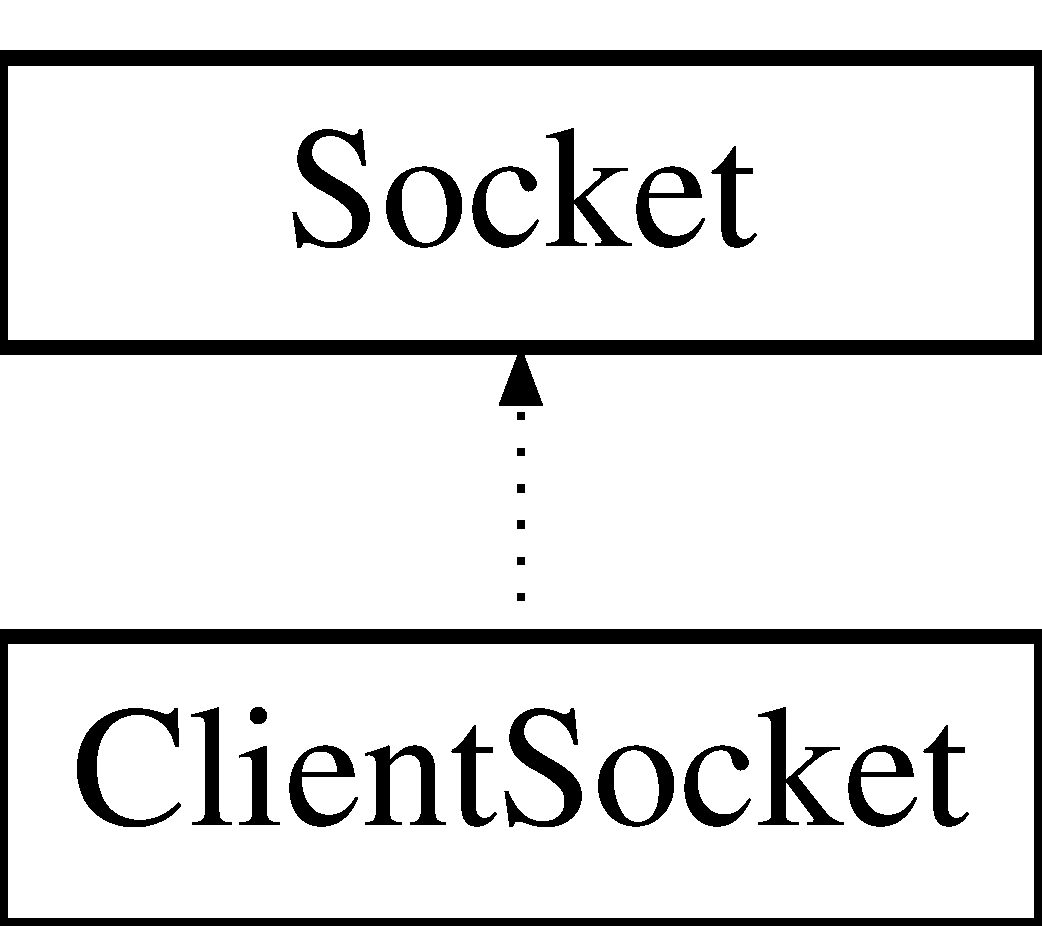
\includegraphics[height=2.000000cm]{class_client_socket}
\end{center}
\end{figure}
\subsection*{Public Member Functions}
\begin{DoxyCompactItemize}
\item 
\hyperlink{class_client_socket_a02809f0ffec549af450364df54175cce}{Client\-Socket} (std\-::string host, int port)
\item 
virtual \hyperlink{class_client_socket_a9c8af4fc4f56b62ef0ff7d67037f65a3}{$\sim$\-Client\-Socket} ()
\item 
const \hyperlink{class_client_socket}{Client\-Socket} \& \hyperlink{class_client_socket_a2fe5c2037ee6bdcc4d578db1111928ba}{operator$<$$<$} (const std\-::string \&) const 
\item 
const \hyperlink{class_client_socket}{Client\-Socket} \& \hyperlink{class_client_socket_a6cb39e9222b501c8b070de60ef6b5fbc}{operator$>$$>$} (std\-::string \&) const 
\end{DoxyCompactItemize}


\subsection{Constructor \& Destructor Documentation}
\hypertarget{class_client_socket_a02809f0ffec549af450364df54175cce}{\index{Client\-Socket@{Client\-Socket}!Client\-Socket@{Client\-Socket}}
\index{Client\-Socket@{Client\-Socket}!ClientSocket@{Client\-Socket}}
\subsubsection[{Client\-Socket}]{\setlength{\rightskip}{0pt plus 5cm}Client\-Socket\-::\-Client\-Socket (
\begin{DoxyParamCaption}
\item[{std\-::string}]{host, }
\item[{int}]{port}
\end{DoxyParamCaption}
)}}\label{class_client_socket_a02809f0ffec549af450364df54175cce}
\hypertarget{class_client_socket_a9c8af4fc4f56b62ef0ff7d67037f65a3}{\index{Client\-Socket@{Client\-Socket}!$\sim$\-Client\-Socket@{$\sim$\-Client\-Socket}}
\index{$\sim$\-Client\-Socket@{$\sim$\-Client\-Socket}!ClientSocket@{Client\-Socket}}
\subsubsection[{$\sim$\-Client\-Socket}]{\setlength{\rightskip}{0pt plus 5cm}virtual Client\-Socket\-::$\sim$\-Client\-Socket (
\begin{DoxyParamCaption}
{}
\end{DoxyParamCaption}
)\hspace{0.3cm}{\ttfamily [inline]}, {\ttfamily [virtual]}}}\label{class_client_socket_a9c8af4fc4f56b62ef0ff7d67037f65a3}


\subsection{Member Function Documentation}
\hypertarget{class_client_socket_a2fe5c2037ee6bdcc4d578db1111928ba}{\index{Client\-Socket@{Client\-Socket}!operator$<$$<$@{operator$<$$<$}}
\index{operator$<$$<$@{operator$<$$<$}!ClientSocket@{Client\-Socket}}
\subsubsection[{operator$<$$<$}]{\setlength{\rightskip}{0pt plus 5cm}const {\bf Client\-Socket} \& Client\-Socket\-::operator$<$$<$ (
\begin{DoxyParamCaption}
\item[{const std\-::string \&}]{s}
\end{DoxyParamCaption}
) const}}\label{class_client_socket_a2fe5c2037ee6bdcc4d578db1111928ba}
\hypertarget{class_client_socket_a6cb39e9222b501c8b070de60ef6b5fbc}{\index{Client\-Socket@{Client\-Socket}!operator$>$$>$@{operator$>$$>$}}
\index{operator$>$$>$@{operator$>$$>$}!ClientSocket@{Client\-Socket}}
\subsubsection[{operator$>$$>$}]{\setlength{\rightskip}{0pt plus 5cm}const {\bf Client\-Socket} \& Client\-Socket\-::operator$>$$>$ (
\begin{DoxyParamCaption}
\item[{std\-::string \&}]{s}
\end{DoxyParamCaption}
) const}}\label{class_client_socket_a6cb39e9222b501c8b070de60ef6b5fbc}


The documentation for this class was generated from the following files\-:\begin{DoxyCompactItemize}
\item 
logic/lanconection/\hyperlink{clientsocket_8h}{clientsocket.\-h}\item 
logic/lanconection/\hyperlink{clientsocket_8cpp}{clientsocket.\-cpp}\end{DoxyCompactItemize}

\hypertarget{class_close}{\section{Close Class Reference}
\label{class_close}\index{Close@{Close}}
}


{\ttfamily \#include $<$Stop.\-pb.\-h$>$}

Inheritance diagram for Close\-:\begin{figure}[H]
\begin{center}
\leavevmode
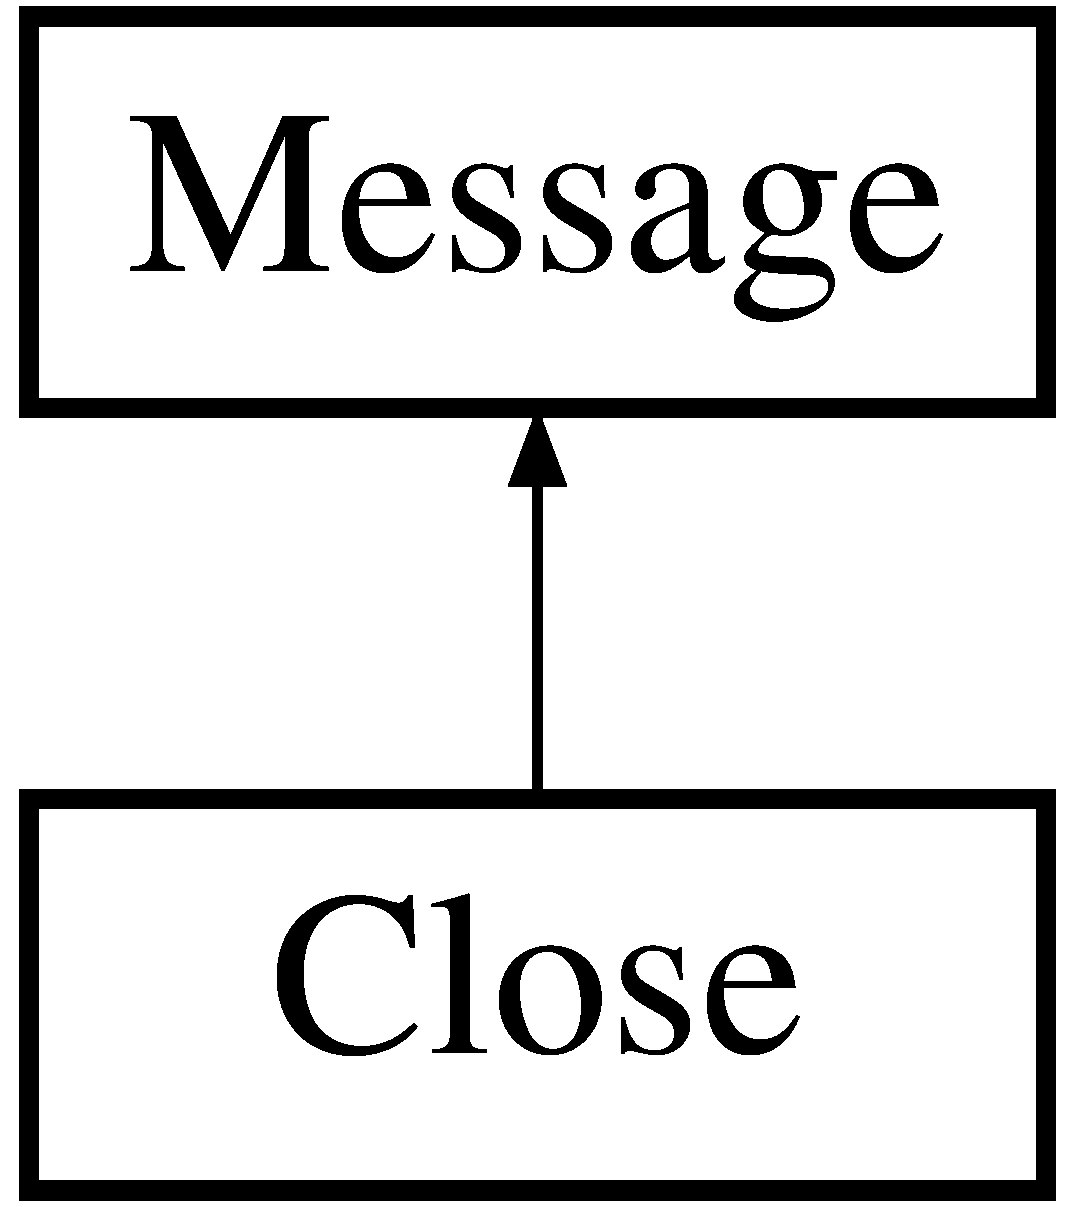
\includegraphics[height=2.000000cm]{class_close}
\end{center}
\end{figure}
\subsection*{Public Member Functions}
\begin{DoxyCompactItemize}
\item 
\hyperlink{class_close_ad8a0a2858285bd127f5f666bed8dc543}{Close} ()
\item 
virtual \hyperlink{class_close_ae0effd9b2f59fb9f2a6dc87104ef11ea}{$\sim$\-Close} ()
\item 
\hyperlink{class_close_a3cf170e3bce53793243f8459409307b7}{Close} (const \hyperlink{class_close}{Close} \&from)
\item 
\hyperlink{class_close}{Close} \& \hyperlink{class_close_a1b25cdc167aee37d7a8309b04d077bad}{operator=} (const \hyperlink{class_close}{Close} \&from)
\item 
const \\*
\-::google\-::protobuf\-::\-Unknown\-Field\-Set \& \hyperlink{class_close_a5be69c428eb1703c4d80eea28c292d29}{unknown\-\_\-fields} () const 
\item 
inline\-::google\-::protobuf\-::\-Unknown\-Field\-Set $\ast$ \hyperlink{class_close_ae28750281fa411c3c3f8f48caf424ab6}{mutable\-\_\-unknown\-\_\-fields} ()
\item 
void \hyperlink{class_close_aa03838e3abc80695ba93ef7739d7d9fc}{Swap} (\hyperlink{class_close}{Close} $\ast$other)
\item 
\hyperlink{class_close}{Close} $\ast$ \hyperlink{class_close_a863cee284bf4ba2e629e53322e79c218}{New} () const 
\item 
\hyperlink{class_close}{Close} $\ast$ \hyperlink{class_close_a93fd428d5681d636ca918d07e15d6550}{New} (\-::google\-::protobuf\-::\-Arena $\ast$arena) const 
\item 
void \hyperlink{class_close_a8b24eba0bd4d8ee9e6dc879941651748}{Copy\-From} (const \-::google\-::protobuf\-::\-Message \&from)
\item 
void \hyperlink{class_close_a94c8f74312a7d33986d44d5195815d2e}{Merge\-From} (const \-::google\-::protobuf\-::\-Message \&from)
\item 
void \hyperlink{class_close_a104d789ceecc954d91da7df0f107779f}{Copy\-From} (const \hyperlink{class_close}{Close} \&from)
\item 
void \hyperlink{class_close_a37c912bb9f92cdfaa33a7ce8d8ee130e}{Merge\-From} (const \hyperlink{class_close}{Close} \&from)
\item 
void \hyperlink{class_close_afda54c6204c3922e74fc47c60a108220}{Clear} ()
\item 
bool \hyperlink{class_close_a5aebc81fadea648480666a41fe66c3cb}{Is\-Initialized} () const 
\item 
int \hyperlink{class_close_a2421ad573317a21c714c039851fa1220}{Byte\-Size} () const 
\item 
bool \hyperlink{class_close_a381c8ce094e6dc74a20400ccbfaea748}{Merge\-Partial\-From\-Coded\-Stream} (\-::google\-::protobuf\-::io\-::\-Coded\-Input\-Stream $\ast$input)
\item 
void \hyperlink{class_close_aeb282667ae1da2dd18c98d7ca711bd88}{Serialize\-With\-Cached\-Sizes} (\-::google\-::protobuf\-::io\-::\-Coded\-Output\-Stream $\ast$output) const 
\item 
\-::google\-::protobuf\-::uint8 $\ast$ \hyperlink{class_close_ac660e547b27cd984e526c0e248c69222}{Serialize\-With\-Cached\-Sizes\-To\-Array} (\-::google\-::protobuf\-::uint8 $\ast$output) const 
\item 
int \hyperlink{class_close_af8b2e8fb8ce9a11e24e63494656a6b28}{Get\-Cached\-Size} () const 
\item 
\-::google\-::protobuf\-::\-Metadata \hyperlink{class_close_a8ce129c6a94a5d6c4b664c6642d1d751}{Get\-Metadata} () const 
\item 
bool \hyperlink{class_close_ac85b7e010a254d4778e91d42fb95ff47}{has\-\_\-close} () const 
\item 
void \hyperlink{class_close_abf4dedd7abc99a939cd94219853b152d}{clear\-\_\-close} ()
\item 
bool \hyperlink{class_close_a300dbccf28dbbcbf9636f197d23bc44a}{close} () const 
\item 
void \hyperlink{class_close_a4557b1b27a9b4934714379e4797ba5c8}{set\-\_\-close} (bool value)
\end{DoxyCompactItemize}
\subsection*{Static Public Member Functions}
\begin{DoxyCompactItemize}
\item 
static const \\*
\-::google\-::protobuf\-::\-Descriptor $\ast$ \hyperlink{class_close_a42a5f68ed3c237f2d54319a4f8e1c5f5}{descriptor} ()
\item 
static const \hyperlink{class_close}{Close} \& \hyperlink{class_close_a90105787bd12a6ac106a06bb39b0b034}{default\-\_\-instance} ()
\end{DoxyCompactItemize}
\subsection*{Static Public Attributes}
\begin{DoxyCompactItemize}
\item 
static const int \hyperlink{class_close_ae10c316a91463074882301092a5c07b1}{k\-Close\-Field\-Number} = 1
\end{DoxyCompactItemize}
\subsection*{Friends}
\begin{DoxyCompactItemize}
\item 
void \hyperlink{class_close_a0c39e7d18f2c161aa57a4cc4b9e6ec8f}{protobuf\-\_\-\-Add\-Desc\-\_\-\-Stop\-\_\-2eproto} ()
\item 
void \hyperlink{class_close_aa2b2a8c14ba7de4972609cfba873a048}{protobuf\-\_\-\-Assign\-Desc\-\_\-\-Stop\-\_\-2eproto} ()
\item 
void \hyperlink{class_close_a286f43855e53704e855ebc2fcc228c04}{protobuf\-\_\-\-Shutdown\-File\-\_\-\-Stop\-\_\-2eproto} ()
\end{DoxyCompactItemize}


\subsection{Constructor \& Destructor Documentation}
\hypertarget{class_close_ad8a0a2858285bd127f5f666bed8dc543}{\index{Close@{Close}!Close@{Close}}
\index{Close@{Close}!Close@{Close}}
\subsubsection[{Close}]{\setlength{\rightskip}{0pt plus 5cm}Close\-::\-Close (
\begin{DoxyParamCaption}
{}
\end{DoxyParamCaption}
)}}\label{class_close_ad8a0a2858285bd127f5f666bed8dc543}
\hypertarget{class_close_ae0effd9b2f59fb9f2a6dc87104ef11ea}{\index{Close@{Close}!$\sim$\-Close@{$\sim$\-Close}}
\index{$\sim$\-Close@{$\sim$\-Close}!Close@{Close}}
\subsubsection[{$\sim$\-Close}]{\setlength{\rightskip}{0pt plus 5cm}Close\-::$\sim$\-Close (
\begin{DoxyParamCaption}
{}
\end{DoxyParamCaption}
)\hspace{0.3cm}{\ttfamily [virtual]}}}\label{class_close_ae0effd9b2f59fb9f2a6dc87104ef11ea}
\hypertarget{class_close_a3cf170e3bce53793243f8459409307b7}{\index{Close@{Close}!Close@{Close}}
\index{Close@{Close}!Close@{Close}}
\subsubsection[{Close}]{\setlength{\rightskip}{0pt plus 5cm}Close\-::\-Close (
\begin{DoxyParamCaption}
\item[{const {\bf Close} \&}]{from}
\end{DoxyParamCaption}
)}}\label{class_close_a3cf170e3bce53793243f8459409307b7}


\subsection{Member Function Documentation}
\hypertarget{class_close_a2421ad573317a21c714c039851fa1220}{\index{Close@{Close}!Byte\-Size@{Byte\-Size}}
\index{Byte\-Size@{Byte\-Size}!Close@{Close}}
\subsubsection[{Byte\-Size}]{\setlength{\rightskip}{0pt plus 5cm}int Close\-::\-Byte\-Size (
\begin{DoxyParamCaption}
{}
\end{DoxyParamCaption}
) const}}\label{class_close_a2421ad573317a21c714c039851fa1220}
\hypertarget{class_close_afda54c6204c3922e74fc47c60a108220}{\index{Close@{Close}!Clear@{Clear}}
\index{Clear@{Clear}!Close@{Close}}
\subsubsection[{Clear}]{\setlength{\rightskip}{0pt plus 5cm}void Close\-::\-Clear (
\begin{DoxyParamCaption}
{}
\end{DoxyParamCaption}
)}}\label{class_close_afda54c6204c3922e74fc47c60a108220}
\hypertarget{class_close_abf4dedd7abc99a939cd94219853b152d}{\index{Close@{Close}!clear\-\_\-close@{clear\-\_\-close}}
\index{clear\-\_\-close@{clear\-\_\-close}!Close@{Close}}
\subsubsection[{clear\-\_\-close}]{\setlength{\rightskip}{0pt plus 5cm}void Close\-::clear\-\_\-close (
\begin{DoxyParamCaption}
{}
\end{DoxyParamCaption}
)\hspace{0.3cm}{\ttfamily [inline]}}}\label{class_close_abf4dedd7abc99a939cd94219853b152d}
\hypertarget{class_close_a300dbccf28dbbcbf9636f197d23bc44a}{\index{Close@{Close}!close@{close}}
\index{close@{close}!Close@{Close}}
\subsubsection[{close}]{\setlength{\rightskip}{0pt plus 5cm}bool Close\-::close (
\begin{DoxyParamCaption}
{}
\end{DoxyParamCaption}
) const\hspace{0.3cm}{\ttfamily [inline]}}}\label{class_close_a300dbccf28dbbcbf9636f197d23bc44a}
\hypertarget{class_close_a8b24eba0bd4d8ee9e6dc879941651748}{\index{Close@{Close}!Copy\-From@{Copy\-From}}
\index{Copy\-From@{Copy\-From}!Close@{Close}}
\subsubsection[{Copy\-From}]{\setlength{\rightskip}{0pt plus 5cm}void Close\-::\-Copy\-From (
\begin{DoxyParamCaption}
\item[{const \-::google\-::protobuf\-::\-Message \&}]{from}
\end{DoxyParamCaption}
)}}\label{class_close_a8b24eba0bd4d8ee9e6dc879941651748}
\hypertarget{class_close_a104d789ceecc954d91da7df0f107779f}{\index{Close@{Close}!Copy\-From@{Copy\-From}}
\index{Copy\-From@{Copy\-From}!Close@{Close}}
\subsubsection[{Copy\-From}]{\setlength{\rightskip}{0pt plus 5cm}void Close\-::\-Copy\-From (
\begin{DoxyParamCaption}
\item[{const {\bf Close} \&}]{from}
\end{DoxyParamCaption}
)}}\label{class_close_a104d789ceecc954d91da7df0f107779f}
\hypertarget{class_close_a90105787bd12a6ac106a06bb39b0b034}{\index{Close@{Close}!default\-\_\-instance@{default\-\_\-instance}}
\index{default\-\_\-instance@{default\-\_\-instance}!Close@{Close}}
\subsubsection[{default\-\_\-instance}]{\setlength{\rightskip}{0pt plus 5cm}const {\bf Close} \& Close\-::default\-\_\-instance (
\begin{DoxyParamCaption}
{}
\end{DoxyParamCaption}
)\hspace{0.3cm}{\ttfamily [static]}}}\label{class_close_a90105787bd12a6ac106a06bb39b0b034}
\hypertarget{class_close_a42a5f68ed3c237f2d54319a4f8e1c5f5}{\index{Close@{Close}!descriptor@{descriptor}}
\index{descriptor@{descriptor}!Close@{Close}}
\subsubsection[{descriptor}]{\setlength{\rightskip}{0pt plus 5cm}const \-::google\-::protobuf\-::\-Descriptor $\ast$ Close\-::descriptor (
\begin{DoxyParamCaption}
{}
\end{DoxyParamCaption}
)\hspace{0.3cm}{\ttfamily [static]}}}\label{class_close_a42a5f68ed3c237f2d54319a4f8e1c5f5}
\hypertarget{class_close_af8b2e8fb8ce9a11e24e63494656a6b28}{\index{Close@{Close}!Get\-Cached\-Size@{Get\-Cached\-Size}}
\index{Get\-Cached\-Size@{Get\-Cached\-Size}!Close@{Close}}
\subsubsection[{Get\-Cached\-Size}]{\setlength{\rightskip}{0pt plus 5cm}int Close\-::\-Get\-Cached\-Size (
\begin{DoxyParamCaption}
{}
\end{DoxyParamCaption}
) const\hspace{0.3cm}{\ttfamily [inline]}}}\label{class_close_af8b2e8fb8ce9a11e24e63494656a6b28}
\hypertarget{class_close_a8ce129c6a94a5d6c4b664c6642d1d751}{\index{Close@{Close}!Get\-Metadata@{Get\-Metadata}}
\index{Get\-Metadata@{Get\-Metadata}!Close@{Close}}
\subsubsection[{Get\-Metadata}]{\setlength{\rightskip}{0pt plus 5cm}google\-::protobuf\-::\-Metadata Close\-::\-Get\-Metadata (
\begin{DoxyParamCaption}
{}
\end{DoxyParamCaption}
) const}}\label{class_close_a8ce129c6a94a5d6c4b664c6642d1d751}
\hypertarget{class_close_ac85b7e010a254d4778e91d42fb95ff47}{\index{Close@{Close}!has\-\_\-close@{has\-\_\-close}}
\index{has\-\_\-close@{has\-\_\-close}!Close@{Close}}
\subsubsection[{has\-\_\-close}]{\setlength{\rightskip}{0pt plus 5cm}bool Close\-::has\-\_\-close (
\begin{DoxyParamCaption}
{}
\end{DoxyParamCaption}
) const\hspace{0.3cm}{\ttfamily [inline]}}}\label{class_close_ac85b7e010a254d4778e91d42fb95ff47}
\hypertarget{class_close_a5aebc81fadea648480666a41fe66c3cb}{\index{Close@{Close}!Is\-Initialized@{Is\-Initialized}}
\index{Is\-Initialized@{Is\-Initialized}!Close@{Close}}
\subsubsection[{Is\-Initialized}]{\setlength{\rightskip}{0pt plus 5cm}bool Close\-::\-Is\-Initialized (
\begin{DoxyParamCaption}
{}
\end{DoxyParamCaption}
) const}}\label{class_close_a5aebc81fadea648480666a41fe66c3cb}
\hypertarget{class_close_a94c8f74312a7d33986d44d5195815d2e}{\index{Close@{Close}!Merge\-From@{Merge\-From}}
\index{Merge\-From@{Merge\-From}!Close@{Close}}
\subsubsection[{Merge\-From}]{\setlength{\rightskip}{0pt plus 5cm}void Close\-::\-Merge\-From (
\begin{DoxyParamCaption}
\item[{const \-::google\-::protobuf\-::\-Message \&}]{from}
\end{DoxyParamCaption}
)}}\label{class_close_a94c8f74312a7d33986d44d5195815d2e}
\hypertarget{class_close_a37c912bb9f92cdfaa33a7ce8d8ee130e}{\index{Close@{Close}!Merge\-From@{Merge\-From}}
\index{Merge\-From@{Merge\-From}!Close@{Close}}
\subsubsection[{Merge\-From}]{\setlength{\rightskip}{0pt plus 5cm}void Close\-::\-Merge\-From (
\begin{DoxyParamCaption}
\item[{const {\bf Close} \&}]{from}
\end{DoxyParamCaption}
)}}\label{class_close_a37c912bb9f92cdfaa33a7ce8d8ee130e}
\hypertarget{class_close_a381c8ce094e6dc74a20400ccbfaea748}{\index{Close@{Close}!Merge\-Partial\-From\-Coded\-Stream@{Merge\-Partial\-From\-Coded\-Stream}}
\index{Merge\-Partial\-From\-Coded\-Stream@{Merge\-Partial\-From\-Coded\-Stream}!Close@{Close}}
\subsubsection[{Merge\-Partial\-From\-Coded\-Stream}]{\setlength{\rightskip}{0pt plus 5cm}bool Close\-::\-Merge\-Partial\-From\-Coded\-Stream (
\begin{DoxyParamCaption}
\item[{\-::google\-::protobuf\-::io\-::\-Coded\-Input\-Stream $\ast$}]{input}
\end{DoxyParamCaption}
)}}\label{class_close_a381c8ce094e6dc74a20400ccbfaea748}
\hypertarget{class_close_ae28750281fa411c3c3f8f48caf424ab6}{\index{Close@{Close}!mutable\-\_\-unknown\-\_\-fields@{mutable\-\_\-unknown\-\_\-fields}}
\index{mutable\-\_\-unknown\-\_\-fields@{mutable\-\_\-unknown\-\_\-fields}!Close@{Close}}
\subsubsection[{mutable\-\_\-unknown\-\_\-fields}]{\setlength{\rightskip}{0pt plus 5cm}inline \-::google\-::protobuf\-::\-Unknown\-Field\-Set$\ast$ Close\-::mutable\-\_\-unknown\-\_\-fields (
\begin{DoxyParamCaption}
{}
\end{DoxyParamCaption}
)\hspace{0.3cm}{\ttfamily [inline]}}}\label{class_close_ae28750281fa411c3c3f8f48caf424ab6}
\hypertarget{class_close_a863cee284bf4ba2e629e53322e79c218}{\index{Close@{Close}!New@{New}}
\index{New@{New}!Close@{Close}}
\subsubsection[{New}]{\setlength{\rightskip}{0pt plus 5cm}{\bf Close}$\ast$ Close\-::\-New (
\begin{DoxyParamCaption}
{}
\end{DoxyParamCaption}
) const\hspace{0.3cm}{\ttfamily [inline]}}}\label{class_close_a863cee284bf4ba2e629e53322e79c218}
\hypertarget{class_close_a93fd428d5681d636ca918d07e15d6550}{\index{Close@{Close}!New@{New}}
\index{New@{New}!Close@{Close}}
\subsubsection[{New}]{\setlength{\rightskip}{0pt plus 5cm}{\bf Close} $\ast$ Close\-::\-New (
\begin{DoxyParamCaption}
\item[{\-::google\-::protobuf\-::\-Arena $\ast$}]{arena}
\end{DoxyParamCaption}
) const}}\label{class_close_a93fd428d5681d636ca918d07e15d6550}
\hypertarget{class_close_a1b25cdc167aee37d7a8309b04d077bad}{\index{Close@{Close}!operator=@{operator=}}
\index{operator=@{operator=}!Close@{Close}}
\subsubsection[{operator=}]{\setlength{\rightskip}{0pt plus 5cm}{\bf Close}\& Close\-::operator= (
\begin{DoxyParamCaption}
\item[{const {\bf Close} \&}]{from}
\end{DoxyParamCaption}
)\hspace{0.3cm}{\ttfamily [inline]}}}\label{class_close_a1b25cdc167aee37d7a8309b04d077bad}
\hypertarget{class_close_aeb282667ae1da2dd18c98d7ca711bd88}{\index{Close@{Close}!Serialize\-With\-Cached\-Sizes@{Serialize\-With\-Cached\-Sizes}}
\index{Serialize\-With\-Cached\-Sizes@{Serialize\-With\-Cached\-Sizes}!Close@{Close}}
\subsubsection[{Serialize\-With\-Cached\-Sizes}]{\setlength{\rightskip}{0pt plus 5cm}void Close\-::\-Serialize\-With\-Cached\-Sizes (
\begin{DoxyParamCaption}
\item[{\-::google\-::protobuf\-::io\-::\-Coded\-Output\-Stream $\ast$}]{output}
\end{DoxyParamCaption}
) const}}\label{class_close_aeb282667ae1da2dd18c98d7ca711bd88}
\hypertarget{class_close_ac660e547b27cd984e526c0e248c69222}{\index{Close@{Close}!Serialize\-With\-Cached\-Sizes\-To\-Array@{Serialize\-With\-Cached\-Sizes\-To\-Array}}
\index{Serialize\-With\-Cached\-Sizes\-To\-Array@{Serialize\-With\-Cached\-Sizes\-To\-Array}!Close@{Close}}
\subsubsection[{Serialize\-With\-Cached\-Sizes\-To\-Array}]{\setlength{\rightskip}{0pt plus 5cm}google\-::protobuf\-::uint8 $\ast$ Close\-::\-Serialize\-With\-Cached\-Sizes\-To\-Array (
\begin{DoxyParamCaption}
\item[{\-::google\-::protobuf\-::uint8 $\ast$}]{output}
\end{DoxyParamCaption}
) const}}\label{class_close_ac660e547b27cd984e526c0e248c69222}
\hypertarget{class_close_a4557b1b27a9b4934714379e4797ba5c8}{\index{Close@{Close}!set\-\_\-close@{set\-\_\-close}}
\index{set\-\_\-close@{set\-\_\-close}!Close@{Close}}
\subsubsection[{set\-\_\-close}]{\setlength{\rightskip}{0pt plus 5cm}void Close\-::set\-\_\-close (
\begin{DoxyParamCaption}
\item[{bool}]{value}
\end{DoxyParamCaption}
)\hspace{0.3cm}{\ttfamily [inline]}}}\label{class_close_a4557b1b27a9b4934714379e4797ba5c8}
\hypertarget{class_close_aa03838e3abc80695ba93ef7739d7d9fc}{\index{Close@{Close}!Swap@{Swap}}
\index{Swap@{Swap}!Close@{Close}}
\subsubsection[{Swap}]{\setlength{\rightskip}{0pt plus 5cm}void Close\-::\-Swap (
\begin{DoxyParamCaption}
\item[{{\bf Close} $\ast$}]{other}
\end{DoxyParamCaption}
)}}\label{class_close_aa03838e3abc80695ba93ef7739d7d9fc}
\hypertarget{class_close_a5be69c428eb1703c4d80eea28c292d29}{\index{Close@{Close}!unknown\-\_\-fields@{unknown\-\_\-fields}}
\index{unknown\-\_\-fields@{unknown\-\_\-fields}!Close@{Close}}
\subsubsection[{unknown\-\_\-fields}]{\setlength{\rightskip}{0pt plus 5cm}const \-::google\-::protobuf\-::\-Unknown\-Field\-Set\& Close\-::unknown\-\_\-fields (
\begin{DoxyParamCaption}
{}
\end{DoxyParamCaption}
) const\hspace{0.3cm}{\ttfamily [inline]}}}\label{class_close_a5be69c428eb1703c4d80eea28c292d29}


\subsection{Friends And Related Function Documentation}
\hypertarget{class_close_a0c39e7d18f2c161aa57a4cc4b9e6ec8f}{\index{Close@{Close}!protobuf\-\_\-\-Add\-Desc\-\_\-\-Stop\-\_\-2eproto@{protobuf\-\_\-\-Add\-Desc\-\_\-\-Stop\-\_\-2eproto}}
\index{protobuf\-\_\-\-Add\-Desc\-\_\-\-Stop\-\_\-2eproto@{protobuf\-\_\-\-Add\-Desc\-\_\-\-Stop\-\_\-2eproto}!Close@{Close}}
\subsubsection[{protobuf\-\_\-\-Add\-Desc\-\_\-\-Stop\-\_\-2eproto}]{\setlength{\rightskip}{0pt plus 5cm}void protobuf\-\_\-\-Add\-Desc\-\_\-\-Stop\-\_\-2eproto (
\begin{DoxyParamCaption}
{}
\end{DoxyParamCaption}
)\hspace{0.3cm}{\ttfamily [friend]}}}\label{class_close_a0c39e7d18f2c161aa57a4cc4b9e6ec8f}
\hypertarget{class_close_aa2b2a8c14ba7de4972609cfba873a048}{\index{Close@{Close}!protobuf\-\_\-\-Assign\-Desc\-\_\-\-Stop\-\_\-2eproto@{protobuf\-\_\-\-Assign\-Desc\-\_\-\-Stop\-\_\-2eproto}}
\index{protobuf\-\_\-\-Assign\-Desc\-\_\-\-Stop\-\_\-2eproto@{protobuf\-\_\-\-Assign\-Desc\-\_\-\-Stop\-\_\-2eproto}!Close@{Close}}
\subsubsection[{protobuf\-\_\-\-Assign\-Desc\-\_\-\-Stop\-\_\-2eproto}]{\setlength{\rightskip}{0pt plus 5cm}void protobuf\-\_\-\-Assign\-Desc\-\_\-\-Stop\-\_\-2eproto (
\begin{DoxyParamCaption}
{}
\end{DoxyParamCaption}
)\hspace{0.3cm}{\ttfamily [friend]}}}\label{class_close_aa2b2a8c14ba7de4972609cfba873a048}
\hypertarget{class_close_a286f43855e53704e855ebc2fcc228c04}{\index{Close@{Close}!protobuf\-\_\-\-Shutdown\-File\-\_\-\-Stop\-\_\-2eproto@{protobuf\-\_\-\-Shutdown\-File\-\_\-\-Stop\-\_\-2eproto}}
\index{protobuf\-\_\-\-Shutdown\-File\-\_\-\-Stop\-\_\-2eproto@{protobuf\-\_\-\-Shutdown\-File\-\_\-\-Stop\-\_\-2eproto}!Close@{Close}}
\subsubsection[{protobuf\-\_\-\-Shutdown\-File\-\_\-\-Stop\-\_\-2eproto}]{\setlength{\rightskip}{0pt plus 5cm}void protobuf\-\_\-\-Shutdown\-File\-\_\-\-Stop\-\_\-2eproto (
\begin{DoxyParamCaption}
{}
\end{DoxyParamCaption}
)\hspace{0.3cm}{\ttfamily [friend]}}}\label{class_close_a286f43855e53704e855ebc2fcc228c04}


\subsection{Member Data Documentation}
\hypertarget{class_close_ae10c316a91463074882301092a5c07b1}{\index{Close@{Close}!k\-Close\-Field\-Number@{k\-Close\-Field\-Number}}
\index{k\-Close\-Field\-Number@{k\-Close\-Field\-Number}!Close@{Close}}
\subsubsection[{k\-Close\-Field\-Number}]{\setlength{\rightskip}{0pt plus 5cm}const int Close\-::k\-Close\-Field\-Number = 1\hspace{0.3cm}{\ttfamily [static]}}}\label{class_close_ae10c316a91463074882301092a5c07b1}


The documentation for this class was generated from the following files\-:\begin{DoxyCompactItemize}
\item 
protobufmessage/\hyperlink{_stop_8pb_8h}{Stop.\-pb.\-h}\item 
protobufmessage/\hyperlink{_stop_8pb_8cc}{Stop.\-pb.\-cc}\end{DoxyCompactItemize}

\hypertarget{class_combustible_box}{\section{Combustible\-Box Class Reference}
\label{class_combustible_box}\index{Combustible\-Box@{Combustible\-Box}}
}


Es la caja que da combustible al jugador, o resta vida si el combustible ha sido consumido por los disparos del jugador(es)  




{\ttfamily \#include $<$combustiblebox.\-h$>$}

Inheritance diagram for Combustible\-Box\-:\begin{figure}[H]
\begin{center}
\leavevmode
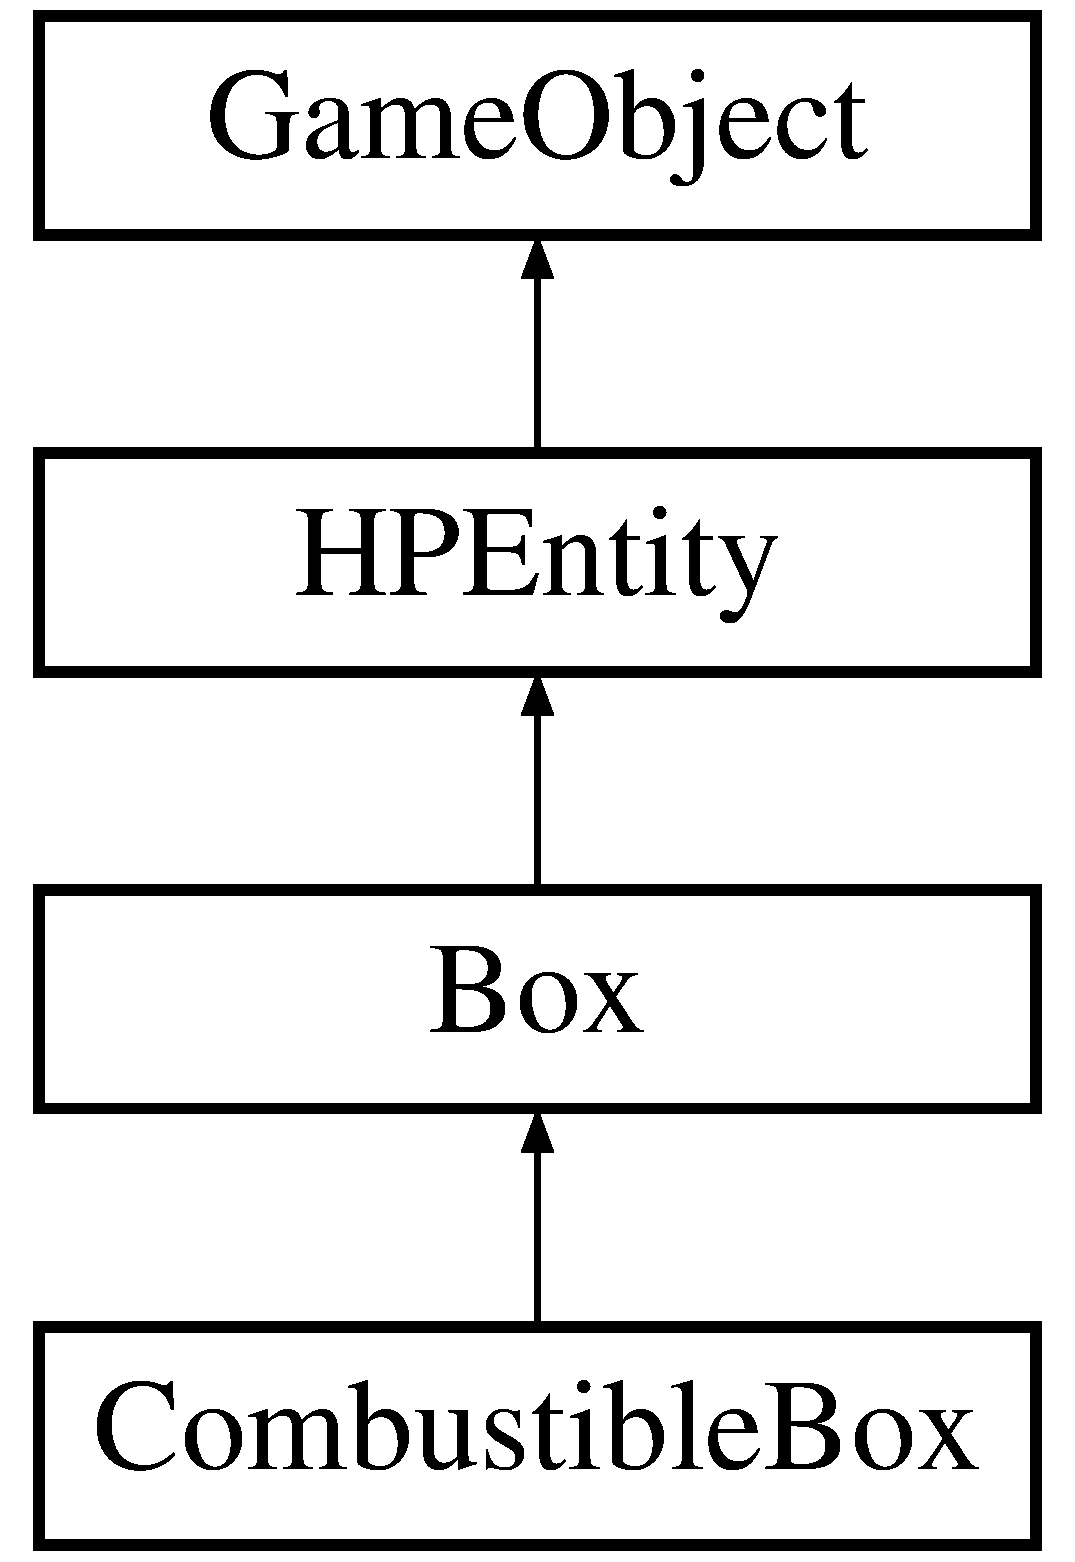
\includegraphics[height=4.000000cm]{class_combustible_box}
\end{center}
\end{figure}
\subsection*{Public Member Functions}
\begin{DoxyCompactItemize}
\item 
\hyperlink{class_combustible_box_abce0b8d39179a5fd5a0fd9076ab25b25}{Combustible\-Box} (Q\-Rect p\-Rect, int p\-Max\-Hp, int p\-Points\-To\-Add)
\begin{DoxyCompactList}\small\item\em Es el constructor de la clase box le da una posicion (x,y) y dimensiones, una cantidad de vida maxima y la cantidad de puntos de combustible que agregara. \end{DoxyCompactList}\item 
void \hyperlink{class_combustible_box_abab14feb7a19ee2a9fc61bbb1a92726a}{add\-Points\-To\-Player} (\hyperlink{class_player}{Player} $\ast$p\-Player)
\begin{DoxyCompactList}\small\item\em Es el metodo que se encarga de sumar el combustible o restar directamente la vida al jugador. \end{DoxyCompactList}\item 
void \hyperlink{class_combustible_box_ac3bcbb721576f4b00b0f2d7e48994657}{update} ()
\begin{DoxyCompactList}\small\item\em Actualiza la posicion de la caja de combustible. \end{DoxyCompactList}\item 
virtual \hyperlink{class_combustible_box_ae16e87f370101cfcd78e7bd763de4620}{$\sim$\-Combustible\-Box} ()
\begin{DoxyCompactList}\small\item\em Destructor de la clase. \end{DoxyCompactList}\end{DoxyCompactItemize}
\subsection*{Additional Inherited Members}


\subsection{Detailed Description}
Es la caja que da combustible al jugador, o resta vida si el combustible ha sido consumido por los disparos del jugador(es) 

\subsection{Constructor \& Destructor Documentation}
\hypertarget{class_combustible_box_abce0b8d39179a5fd5a0fd9076ab25b25}{\index{Combustible\-Box@{Combustible\-Box}!Combustible\-Box@{Combustible\-Box}}
\index{Combustible\-Box@{Combustible\-Box}!CombustibleBox@{Combustible\-Box}}
\subsubsection[{Combustible\-Box}]{\setlength{\rightskip}{0pt plus 5cm}Combustible\-Box\-::\-Combustible\-Box (
\begin{DoxyParamCaption}
\item[{Q\-Rect}]{p\-Rect, }
\item[{int}]{p\-Max\-Hp, }
\item[{int}]{p\-Points\-To\-Add}
\end{DoxyParamCaption}
)}}\label{class_combustible_box_abce0b8d39179a5fd5a0fd9076ab25b25}


Es el constructor de la clase box le da una posicion (x,y) y dimensiones, una cantidad de vida maxima y la cantidad de puntos de combustible que agregara. 


\begin{DoxyParams}{Parameters}
{\em p\-Rect} & Es el rectangulo que contiene la posicion y las dimensiones de la caja \\
\hline
{\em p\-Max\-Hp} & es la cantidad de vida maxima que esta contiene \\
\hline
{\em p\-Points\-To\-Add} & es la cantidad de combustible que se agregara o sustreara del jugador \\
\hline
\end{DoxyParams}
\hypertarget{class_combustible_box_ae16e87f370101cfcd78e7bd763de4620}{\index{Combustible\-Box@{Combustible\-Box}!$\sim$\-Combustible\-Box@{$\sim$\-Combustible\-Box}}
\index{$\sim$\-Combustible\-Box@{$\sim$\-Combustible\-Box}!CombustibleBox@{Combustible\-Box}}
\subsubsection[{$\sim$\-Combustible\-Box}]{\setlength{\rightskip}{0pt plus 5cm}Combustible\-Box\-::$\sim$\-Combustible\-Box (
\begin{DoxyParamCaption}
{}
\end{DoxyParamCaption}
)\hspace{0.3cm}{\ttfamily [virtual]}}}\label{class_combustible_box_ae16e87f370101cfcd78e7bd763de4620}


Destructor de la clase. 



\subsection{Member Function Documentation}
\hypertarget{class_combustible_box_abab14feb7a19ee2a9fc61bbb1a92726a}{\index{Combustible\-Box@{Combustible\-Box}!add\-Points\-To\-Player@{add\-Points\-To\-Player}}
\index{add\-Points\-To\-Player@{add\-Points\-To\-Player}!CombustibleBox@{Combustible\-Box}}
\subsubsection[{add\-Points\-To\-Player}]{\setlength{\rightskip}{0pt plus 5cm}void Combustible\-Box\-::add\-Points\-To\-Player (
\begin{DoxyParamCaption}
\item[{{\bf Player} $\ast$}]{p\-Player}
\end{DoxyParamCaption}
)\hspace{0.3cm}{\ttfamily [virtual]}}}\label{class_combustible_box_abab14feb7a19ee2a9fc61bbb1a92726a}


Es el metodo que se encarga de sumar el combustible o restar directamente la vida al jugador. 


\begin{DoxyParams}{Parameters}
{\em p\-Player} & es el jugador al que se le aplica la operacion de suma o resta de vida o combustible \\
\hline
\end{DoxyParams}


Reimplemented from \hyperlink{class_box_a536c605982fc2000fbda0388d0a2fb2b}{Box}.

\hypertarget{class_combustible_box_ac3bcbb721576f4b00b0f2d7e48994657}{\index{Combustible\-Box@{Combustible\-Box}!update@{update}}
\index{update@{update}!CombustibleBox@{Combustible\-Box}}
\subsubsection[{update}]{\setlength{\rightskip}{0pt plus 5cm}void Combustible\-Box\-::update (
\begin{DoxyParamCaption}
{}
\end{DoxyParamCaption}
)\hspace{0.3cm}{\ttfamily [virtual]}}}\label{class_combustible_box_ac3bcbb721576f4b00b0f2d7e48994657}


Actualiza la posicion de la caja de combustible. 



Reimplemented from \hyperlink{class_box_a779104150a6f06da2bf1500489a58530}{Box}.



The documentation for this class was generated from the following files\-:\begin{DoxyCompactItemize}
\item 
logic/mapobjects/\hyperlink{combustiblebox_8h}{combustiblebox.\-h}\item 
logic/mapobjects/\hyperlink{combustiblebox_8cpp}{combustiblebox.\-cpp}\end{DoxyCompactItemize}

\hypertarget{class_comparer}{\section{Comparer Class Reference}
\label{class_comparer}\index{Comparer@{Comparer}}
}


The documentation for this class was generated from the following files\-:\begin{DoxyCompactItemize}
\item 
ordinate\-List/comparer.\-h\item 
ordinate\-List/comparer.\-cpp\end{DoxyCompactItemize}

\hypertarget{class_connection_manager}{\section{Connection\-Manager Class Reference}
\label{class_connection_manager}\index{Connection\-Manager@{Connection\-Manager}}
}


The documentation for this class was generated from the following files\-:\begin{DoxyCompactItemize}
\item 
logic/lanconection/connectionmanager.\-h\item 
logic/lanconection/connectionmanager.\-cpp\end{DoxyCompactItemize}

\hypertarget{class_control_player}{\section{Control\-Player Class Reference}
\label{class_control_player}\index{Control\-Player@{Control\-Player}}
}
Inheritance diagram for Control\-Player\-:\begin{figure}[H]
\begin{center}
\leavevmode
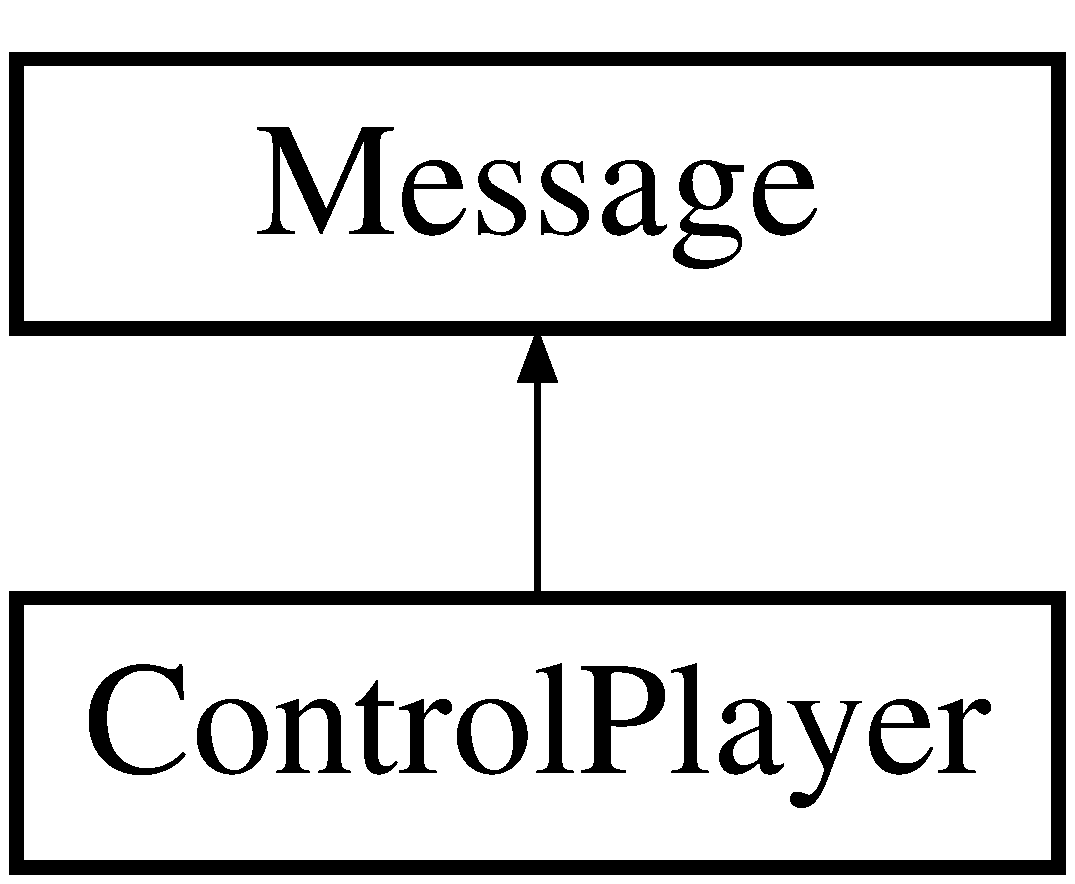
\includegraphics[height=2.000000cm]{class_control_player}
\end{center}
\end{figure}
\subsection*{Public Member Functions}
\begin{DoxyCompactItemize}
\item 
\hypertarget{class_control_player_a4773258dff369c3e618f22915b1ed13c}{{\bfseries Control\-Player} (const \hyperlink{class_control_player}{Control\-Player} \&from)}\label{class_control_player_a4773258dff369c3e618f22915b1ed13c}

\item 
\hypertarget{class_control_player_a1b20164c45224aebee88352c86399be7}{\hyperlink{class_control_player}{Control\-Player} \& {\bfseries operator=} (const \hyperlink{class_control_player}{Control\-Player} \&from)}\label{class_control_player_a1b20164c45224aebee88352c86399be7}

\item 
\hypertarget{class_control_player_ae234e293c6d038e29ac6b84d5fa51130}{const \\*
\-::google\-::protobuf\-::\-Unknown\-Field\-Set \& {\bfseries unknown\-\_\-fields} () const }\label{class_control_player_ae234e293c6d038e29ac6b84d5fa51130}

\item 
\hypertarget{class_control_player_a23294302f5acd784da03d52c49a2c058}{inline\-::google\-::protobuf\-::\-Unknown\-Field\-Set $\ast$ {\bfseries mutable\-\_\-unknown\-\_\-fields} ()}\label{class_control_player_a23294302f5acd784da03d52c49a2c058}

\item 
\hypertarget{class_control_player_a31c6357a93fa21c6739f93bb34c17f78}{void {\bfseries Swap} (\hyperlink{class_control_player}{Control\-Player} $\ast$other)}\label{class_control_player_a31c6357a93fa21c6739f93bb34c17f78}

\item 
\hypertarget{class_control_player_af57ac2d2518b280356cf9d97fe9d7715}{\hyperlink{class_control_player}{Control\-Player} $\ast$ {\bfseries New} () const }\label{class_control_player_af57ac2d2518b280356cf9d97fe9d7715}

\item 
\hypertarget{class_control_player_a693bcd1bbe06f676166d5a39331cc198}{\hyperlink{class_control_player}{Control\-Player} $\ast$ {\bfseries New} (\-::google\-::protobuf\-::\-Arena $\ast$arena) const }\label{class_control_player_a693bcd1bbe06f676166d5a39331cc198}

\item 
\hypertarget{class_control_player_a10ddf43b10f0fc2578bd5ca37d426ed2}{void {\bfseries Copy\-From} (const \-::google\-::protobuf\-::\-Message \&from)}\label{class_control_player_a10ddf43b10f0fc2578bd5ca37d426ed2}

\item 
\hypertarget{class_control_player_ae2e6bf23c72d1c1fafdb4069a0c85616}{void {\bfseries Merge\-From} (const \-::google\-::protobuf\-::\-Message \&from)}\label{class_control_player_ae2e6bf23c72d1c1fafdb4069a0c85616}

\item 
\hypertarget{class_control_player_a3c2ca9aebf93722e016221c52b733e3b}{void {\bfseries Copy\-From} (const \hyperlink{class_control_player}{Control\-Player} \&from)}\label{class_control_player_a3c2ca9aebf93722e016221c52b733e3b}

\item 
\hypertarget{class_control_player_a7c875ed4b63747d865fb668b50ef7b50}{void {\bfseries Merge\-From} (const \hyperlink{class_control_player}{Control\-Player} \&from)}\label{class_control_player_a7c875ed4b63747d865fb668b50ef7b50}

\item 
\hypertarget{class_control_player_a691b54dd8fd3532aa7cb76b84ed85cd5}{void {\bfseries Clear} ()}\label{class_control_player_a691b54dd8fd3532aa7cb76b84ed85cd5}

\item 
\hypertarget{class_control_player_af517c65f7b59b1c11135d462d3df655c}{bool {\bfseries Is\-Initialized} () const }\label{class_control_player_af517c65f7b59b1c11135d462d3df655c}

\item 
\hypertarget{class_control_player_a67b9268037ffaa3b2403fe0539069a4f}{int {\bfseries Byte\-Size} () const }\label{class_control_player_a67b9268037ffaa3b2403fe0539069a4f}

\item 
\hypertarget{class_control_player_adc67bdb8e86fdd28c772e3291218e81b}{bool {\bfseries Merge\-Partial\-From\-Coded\-Stream} (\-::google\-::protobuf\-::io\-::\-Coded\-Input\-Stream $\ast$input)}\label{class_control_player_adc67bdb8e86fdd28c772e3291218e81b}

\item 
\hypertarget{class_control_player_a3f100d88daae100fdbae3ee409fd2359}{void {\bfseries Serialize\-With\-Cached\-Sizes} (\-::google\-::protobuf\-::io\-::\-Coded\-Output\-Stream $\ast$output) const }\label{class_control_player_a3f100d88daae100fdbae3ee409fd2359}

\item 
\hypertarget{class_control_player_a95c6688447829b02a72265eabe54abdb}{\-::google\-::protobuf\-::uint8 $\ast$ {\bfseries Serialize\-With\-Cached\-Sizes\-To\-Array} (\-::google\-::protobuf\-::uint8 $\ast$output) const }\label{class_control_player_a95c6688447829b02a72265eabe54abdb}

\item 
\hypertarget{class_control_player_a286ce6080af5efae2c5769d8904a0d9a}{int {\bfseries Get\-Cached\-Size} () const }\label{class_control_player_a286ce6080af5efae2c5769d8904a0d9a}

\item 
\hypertarget{class_control_player_a6b3b68636b9e666518c5b8c6411bc6cb}{\-::google\-::protobuf\-::\-Metadata {\bfseries Get\-Metadata} () const }\label{class_control_player_a6b3b68636b9e666518c5b8c6411bc6cb}

\item 
\hypertarget{class_control_player_ad9ba495fb6558cb8bcd24be096cbdefa}{bool {\bfseries has\-\_\-num\-\_\-of\-\_\-player} () const }\label{class_control_player_ad9ba495fb6558cb8bcd24be096cbdefa}

\item 
\hypertarget{class_control_player_a24c464ffc2da4acaae33a52e31a1f053}{void {\bfseries clear\-\_\-num\-\_\-of\-\_\-player} ()}\label{class_control_player_a24c464ffc2da4acaae33a52e31a1f053}

\item 
\hypertarget{class_control_player_ac2838f802a27d8c3cde6aae50aa1beb1}{inline\-::google\-::protobuf\-::int32 {\bfseries num\-\_\-of\-\_\-player} () const }\label{class_control_player_ac2838f802a27d8c3cde6aae50aa1beb1}

\item 
\hypertarget{class_control_player_ac6572d26fc4233c40b9194c16fd9a7b4}{void {\bfseries set\-\_\-num\-\_\-of\-\_\-player} (\-::google\-::protobuf\-::int32 value)}\label{class_control_player_ac6572d26fc4233c40b9194c16fd9a7b4}

\item 
\hypertarget{class_control_player_a7b7924fb3150a0185246e9586715f69e}{bool {\bfseries has\-\_\-xvelocity} () const }\label{class_control_player_a7b7924fb3150a0185246e9586715f69e}

\item 
\hypertarget{class_control_player_afb00a137d204116ef3e2ad739e1784e1}{void {\bfseries clear\-\_\-xvelocity} ()}\label{class_control_player_afb00a137d204116ef3e2ad739e1784e1}

\item 
\hypertarget{class_control_player_aa4ae47b09a2afa53a42520d676509af9}{inline\-::google\-::protobuf\-::int32 {\bfseries xvelocity} () const }\label{class_control_player_aa4ae47b09a2afa53a42520d676509af9}

\item 
\hypertarget{class_control_player_a4ad42d15731a8d10bd818631268a0c34}{void {\bfseries set\-\_\-xvelocity} (\-::google\-::protobuf\-::int32 value)}\label{class_control_player_a4ad42d15731a8d10bd818631268a0c34}

\item 
\hypertarget{class_control_player_ad5d47c980b16fa21b4a1e03289f8e219}{bool {\bfseries has\-\_\-yvelocity} () const }\label{class_control_player_ad5d47c980b16fa21b4a1e03289f8e219}

\item 
\hypertarget{class_control_player_a939a11128c7ed1dfaead4df0795744c8}{void {\bfseries clear\-\_\-yvelocity} ()}\label{class_control_player_a939a11128c7ed1dfaead4df0795744c8}

\item 
\hypertarget{class_control_player_a7a039c8d2f85af678def3327245d3d80}{inline\-::google\-::protobuf\-::int32 {\bfseries yvelocity} () const }\label{class_control_player_a7a039c8d2f85af678def3327245d3d80}

\item 
\hypertarget{class_control_player_a901e221ed999443269b1e5495716ff68}{void {\bfseries set\-\_\-yvelocity} (\-::google\-::protobuf\-::int32 value)}\label{class_control_player_a901e221ed999443269b1e5495716ff68}

\item 
\hypertarget{class_control_player_a3d6e80ba43b0603ecdbd762f74810bab}{bool {\bfseries has\-\_\-shoot} () const }\label{class_control_player_a3d6e80ba43b0603ecdbd762f74810bab}

\item 
\hypertarget{class_control_player_a1cf53b17bf67474479aa8444df4ad867}{void {\bfseries clear\-\_\-shoot} ()}\label{class_control_player_a1cf53b17bf67474479aa8444df4ad867}

\item 
\hypertarget{class_control_player_a6f14f0e60e6bc7f736f16502a5a7025e}{bool {\bfseries shoot} () const }\label{class_control_player_a6f14f0e60e6bc7f736f16502a5a7025e}

\item 
\hypertarget{class_control_player_ad26250cc76bd9016bb9136535ea27e5b}{void {\bfseries set\-\_\-shoot} (bool value)}\label{class_control_player_ad26250cc76bd9016bb9136535ea27e5b}

\item 
\hypertarget{class_control_player_a431c723d3d093f961c651fb7947e99c4}{bool {\bfseries has\-\_\-pause} () const }\label{class_control_player_a431c723d3d093f961c651fb7947e99c4}

\item 
\hypertarget{class_control_player_af84ad71ae32b4fa43a1f6263e28783aa}{void {\bfseries clear\-\_\-pause} ()}\label{class_control_player_af84ad71ae32b4fa43a1f6263e28783aa}

\item 
\hypertarget{class_control_player_a549f93f53e0775162cc5d0d5d2cb1da8}{bool {\bfseries pause} () const }\label{class_control_player_a549f93f53e0775162cc5d0d5d2cb1da8}

\item 
\hypertarget{class_control_player_a1c8b853b906342b1c1b9ce15add0721d}{void {\bfseries set\-\_\-pause} (bool value)}\label{class_control_player_a1c8b853b906342b1c1b9ce15add0721d}

\item 
\hypertarget{class_control_player_a106aabf9080b2b4f0cb394c7eaa0cd2a}{bool {\bfseries has\-\_\-changemunition} () const }\label{class_control_player_a106aabf9080b2b4f0cb394c7eaa0cd2a}

\item 
\hypertarget{class_control_player_a4a1f53c88470a7ac2978a3575d5e92d5}{void {\bfseries clear\-\_\-changemunition} ()}\label{class_control_player_a4a1f53c88470a7ac2978a3575d5e92d5}

\item 
\hypertarget{class_control_player_a0010c94deab35537f06b77bb4a7ebc18}{bool {\bfseries changemunition} () const }\label{class_control_player_a0010c94deab35537f06b77bb4a7ebc18}

\item 
\hypertarget{class_control_player_ab22d1f02d208e63cd9a4bcfa20de3562}{void {\bfseries set\-\_\-changemunition} (bool value)}\label{class_control_player_ab22d1f02d208e63cd9a4bcfa20de3562}

\end{DoxyCompactItemize}
\subsection*{Static Public Member Functions}
\begin{DoxyCompactItemize}
\item 
\hypertarget{class_control_player_ac3b3c90e46a07ecabac236d5fd86ad2e}{static const \\*
\-::google\-::protobuf\-::\-Descriptor $\ast$ {\bfseries descriptor} ()}\label{class_control_player_ac3b3c90e46a07ecabac236d5fd86ad2e}

\item 
\hypertarget{class_control_player_ad03d0efd3008b639c64e3b2d09446f66}{static const \hyperlink{class_control_player}{Control\-Player} \& {\bfseries default\-\_\-instance} ()}\label{class_control_player_ad03d0efd3008b639c64e3b2d09446f66}

\end{DoxyCompactItemize}
\subsection*{Static Public Attributes}
\begin{DoxyCompactItemize}
\item 
\hypertarget{class_control_player_aa22557ce6425dad4cb9bbee1c72ea009}{static const int {\bfseries k\-N\-U\-M\-O\-F\-P\-L\-A\-Y\-E\-R\-Field\-Number} = 1}\label{class_control_player_aa22557ce6425dad4cb9bbee1c72ea009}

\item 
\hypertarget{class_control_player_a2848d79ede088ee9d60163a1ce3debb5}{static const int {\bfseries k\-X\-Velocity\-Field\-Number} = 2}\label{class_control_player_a2848d79ede088ee9d60163a1ce3debb5}

\item 
\hypertarget{class_control_player_a23d77701b2b3c5dcac4c23346e3d8008}{static const int {\bfseries k\-Y\-Velocity\-Field\-Number} = 3}\label{class_control_player_a23d77701b2b3c5dcac4c23346e3d8008}

\item 
\hypertarget{class_control_player_a110d46cbecf8ad2123381abec49cd20e}{static const int {\bfseries k\-Shoot\-Field\-Number} = 4}\label{class_control_player_a110d46cbecf8ad2123381abec49cd20e}

\item 
\hypertarget{class_control_player_a5172a9b73b225248c7b0cbc66da6d82a}{static const int {\bfseries k\-Pause\-Field\-Number} = 5}\label{class_control_player_a5172a9b73b225248c7b0cbc66da6d82a}

\item 
\hypertarget{class_control_player_a36f1942f704fa75ce19b13c1d19f9f26}{static const int {\bfseries k\-Change\-Munition\-Field\-Number} = 6}\label{class_control_player_a36f1942f704fa75ce19b13c1d19f9f26}

\end{DoxyCompactItemize}
\subsection*{Friends}
\begin{DoxyCompactItemize}
\item 
\hypertarget{class_control_player_aac621462a97f97bc512d44b05584fdf5}{void {\bfseries protobuf\-\_\-\-Add\-Desc\-\_\-\-Control\-Player\-\_\-2eproto} ()}\label{class_control_player_aac621462a97f97bc512d44b05584fdf5}

\item 
\hypertarget{class_control_player_a21a35d7e412b7505004e6d3230169a28}{void {\bfseries protobuf\-\_\-\-Assign\-Desc\-\_\-\-Control\-Player\-\_\-2eproto} ()}\label{class_control_player_a21a35d7e412b7505004e6d3230169a28}

\item 
\hypertarget{class_control_player_ae1feb442f59225a94fe4948ff34349a6}{void {\bfseries protobuf\-\_\-\-Shutdown\-File\-\_\-\-Control\-Player\-\_\-2eproto} ()}\label{class_control_player_ae1feb442f59225a94fe4948ff34349a6}

\end{DoxyCompactItemize}


The documentation for this class was generated from the following files\-:\begin{DoxyCompactItemize}
\item 
protobufmessage/Control\-Player.\-pb.\-h\item 
protobufmessage/Control\-Player.\-pb.\-cc\end{DoxyCompactItemize}

\hypertarget{class_crazy_river_ride}{\section{Crazy\-River\-Ride Class Reference}
\label{class_crazy_river_ride}\index{Crazy\-River\-Ride@{Crazy\-River\-Ride}}
}
Inheritance diagram for Crazy\-River\-Ride\-:\begin{figure}[H]
\begin{center}
\leavevmode
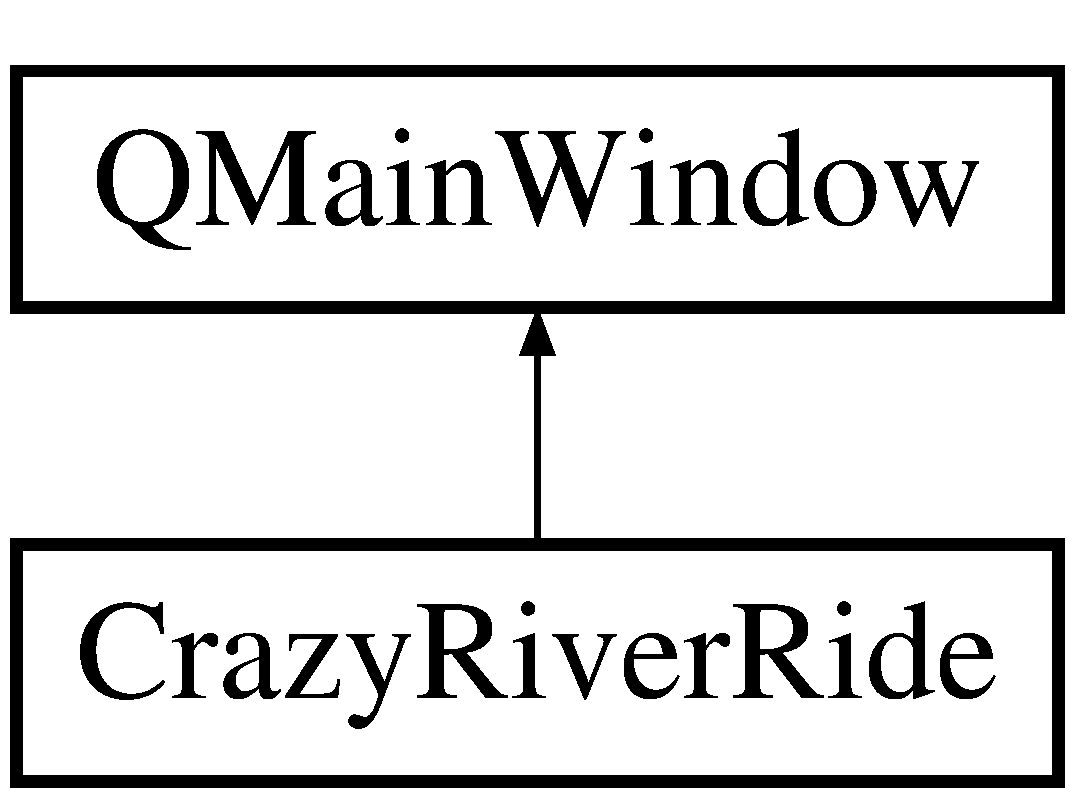
\includegraphics[height=2.000000cm]{class_crazy_river_ride}
\end{center}
\end{figure}
\subsection*{Public Slots}
\begin{DoxyCompactItemize}
\item 
\hypertarget{class_crazy_river_ride_a723a8b3355778a13d7d1e3a3e45d30a0}{void {\bfseries render} ()}\label{class_crazy_river_ride_a723a8b3355778a13d7d1e3a3e45d30a0}

\end{DoxyCompactItemize}
\subsection*{Public Member Functions}
\begin{DoxyCompactItemize}
\item 
\hypertarget{class_crazy_river_ride_ae7676b37caf1b9f9687eb1de0b426b77}{{\bfseries Crazy\-River\-Ride} (Q\-Widget $\ast$parent=0)}\label{class_crazy_river_ride_ae7676b37caf1b9f9687eb1de0b426b77}

\item 
\hypertarget{class_crazy_river_ride_a6f69c5acd7124489c8e95024debec646}{void {\bfseries paint\-Image} (Q\-Rect rec, Q\-Pixmap $\ast$p\-Image)}\label{class_crazy_river_ride_a6f69c5acd7124489c8e95024debec646}

\item 
\hypertarget{class_crazy_river_ride_a915fc6fab259b6fa24b09e64b7710e9c}{int {\bfseries get\-Key\-Xaxis} ()}\label{class_crazy_river_ride_a915fc6fab259b6fa24b09e64b7710e9c}

\item 
\hypertarget{class_crazy_river_ride_a175a99b902ffc945943acc281fb28165}{int {\bfseries get\-Key\-Yaxis} ()}\label{class_crazy_river_ride_a175a99b902ffc945943acc281fb28165}

\item 
\hypertarget{class_crazy_river_ride_ab19f0f54728bec4069aa4c20e547be3c}{bool {\bfseries is\-Running} ()}\label{class_crazy_river_ride_ab19f0f54728bec4069aa4c20e547be3c}

\item 
\hypertarget{class_crazy_river_ride_a25bba6ef360d73e9bd2b43157f0eea0f}{void {\bfseries setkey\-Updater} (\hyperlink{class_key_updater}{Key\-Updater} p\-Key\-Updater)}\label{class_crazy_river_ride_a25bba6ef360d73e9bd2b43157f0eea0f}

\item 
\hypertarget{class_crazy_river_ride_a8e04c2ebe8c0397fada83df2bd736a80}{int {\bfseries get\-Playerlife} () const }\label{class_crazy_river_ride_a8e04c2ebe8c0397fada83df2bd736a80}

\item 
\hypertarget{class_crazy_river_ride_a6314d065ea228fd3464d41989ea56d69}{void {\bfseries set\-Playerlife} (int value)}\label{class_crazy_river_ride_a6314d065ea228fd3464d41989ea56d69}

\item 
\hypertarget{class_crazy_river_ride_a5c94c18d81438b715178bf4d27db79ac}{int {\bfseries get\-Playerpoints} () const }\label{class_crazy_river_ride_a5c94c18d81438b715178bf4d27db79ac}

\item 
\hypertarget{class_crazy_river_ride_ae422c0571f910c124ed96c680892d19b}{void {\bfseries set\-Playerpoints} (int value)}\label{class_crazy_river_ride_ae422c0571f910c124ed96c680892d19b}

\item 
\hypertarget{class_crazy_river_ride_adab75d641f8df41b15851c0139b37cd3}{int {\bfseries get\-Playermunition} () const }\label{class_crazy_river_ride_adab75d641f8df41b15851c0139b37cd3}

\item 
\hypertarget{class_crazy_river_ride_ae773c56d054fd73adadf6f2ab3e725e1}{void {\bfseries set\-Playermunition} (int value)}\label{class_crazy_river_ride_ae773c56d054fd73adadf6f2ab3e725e1}

\item 
\hypertarget{class_crazy_river_ride_a33d1c49da5c75f486a5a6cf468ea194d}{void {\bfseries set\-Renderin\-Type} (bool is\-On\-Menu, bool is\-Game\-Over)}\label{class_crazy_river_ride_a33d1c49da5c75f486a5a6cf468ea194d}

\item 
\hypertarget{class_crazy_river_ride_a7ff417550948dd28d538e614fd23d91b}{int {\bfseries get\-Player\-Combustible} () const }\label{class_crazy_river_ride_a7ff417550948dd28d538e614fd23d91b}

\item 
\hypertarget{class_crazy_river_ride_ab9d581ecdc75251102d8c243d47fbe00}{void {\bfseries set\-Player\-Combustible} (int value)}\label{class_crazy_river_ride_ab9d581ecdc75251102d8c243d47fbe00}

\item 
\hypertarget{class_crazy_river_ride_a48c19baeb07b2e81d2663adc70ede714}{void {\bfseries playmusic} ()}\label{class_crazy_river_ride_a48c19baeb07b2e81d2663adc70ede714}

\end{DoxyCompactItemize}
\subsection*{Protected Member Functions}
\begin{DoxyCompactItemize}
\item 
\hypertarget{class_crazy_river_ride_a1b5346e20df6444e9cdd3e3c978d6a67}{void {\bfseries close\-Event} (Q\-Close\-Event $\ast$)}\label{class_crazy_river_ride_a1b5346e20df6444e9cdd3e3c978d6a67}

\item 
\hypertarget{class_crazy_river_ride_a8a163207bf92442bdfe0ea382d6e7e7d}{void {\bfseries paint\-Event} (Q\-Paint\-Event $\ast$)}\label{class_crazy_river_ride_a8a163207bf92442bdfe0ea382d6e7e7d}

\item 
\hypertarget{class_crazy_river_ride_a87f27420c335b9b693e7dcfe8e0c3281}{void {\bfseries key\-Press\-Event} (Q\-Key\-Event $\ast$)}\label{class_crazy_river_ride_a87f27420c335b9b693e7dcfe8e0c3281}

\item 
\hypertarget{class_crazy_river_ride_af0846544ef52af8e9f7476fa9f7f2f73}{void {\bfseries key\-Release\-Event} (Q\-Key\-Event $\ast$)}\label{class_crazy_river_ride_af0846544ef52af8e9f7476fa9f7f2f73}

\end{DoxyCompactItemize}


The documentation for this class was generated from the following files\-:\begin{DoxyCompactItemize}
\item 
crazyriverride.\-h\item 
crazyriverride.\-cpp\end{DoxyCompactItemize}

\hypertarget{class_crazy_thread}{\section{Crazy\-Thread Class Reference}
\label{class_crazy_thread}\index{Crazy\-Thread@{Crazy\-Thread}}
}


Clase superior no instanciable que representa a los thread del proyecto Crazy River Ride la implementacion de esta clase esta inspirada en la clase que se puede apreciar el en siguiente link.  




{\ttfamily \#include $<$crazythread.\-h$>$}

Inheritance diagram for Crazy\-Thread\-:\begin{figure}[H]
\begin{center}
\leavevmode
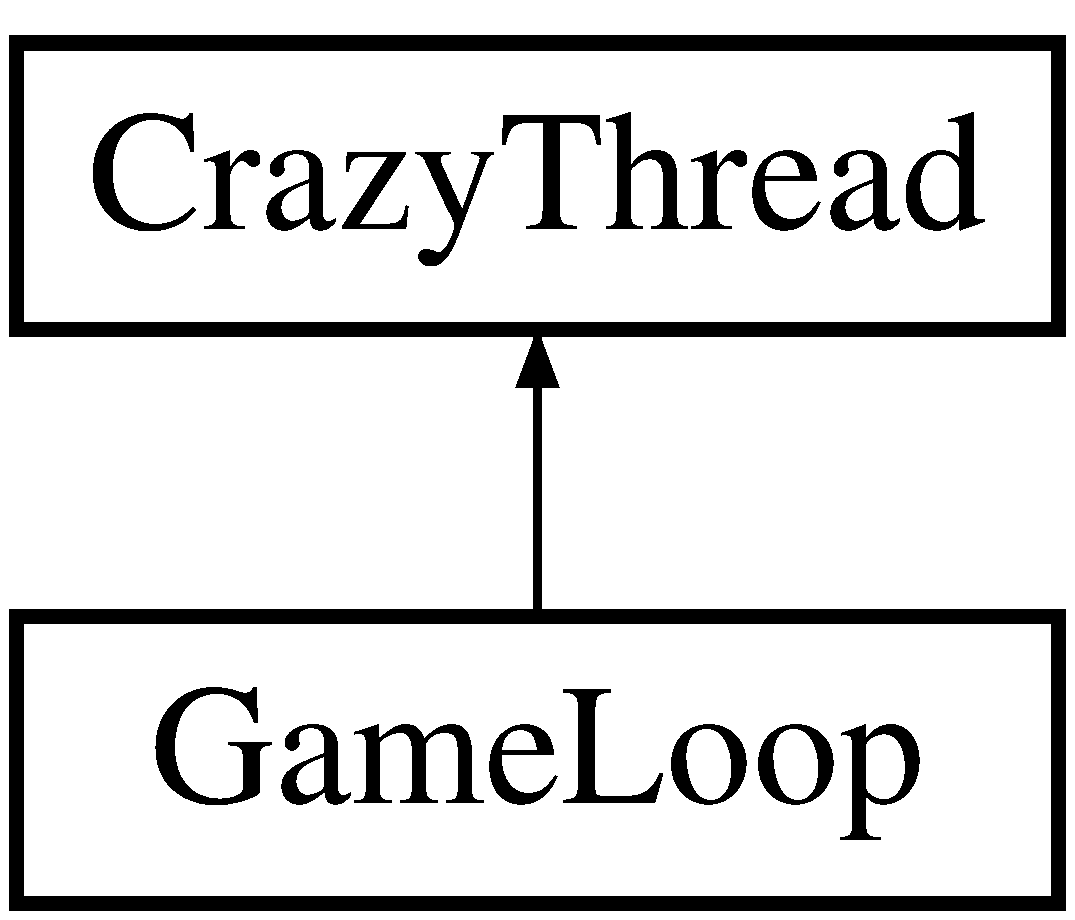
\includegraphics[height=2.000000cm]{class_crazy_thread}
\end{center}
\end{figure}
\subsection*{Public Member Functions}
\begin{DoxyCompactItemize}
\item 
\hyperlink{class_crazy_thread_a0e0ca1644ff99dc033d11a58e0e54cd8}{Crazy\-Thread} ()
\begin{DoxyCompactList}\small\item\em Constructor de la clase, es el constructor por defecto. \end{DoxyCompactList}\item 
virtual \hyperlink{class_crazy_thread_a46e62f5a5f328d329b5b14edc693fd77}{$\sim$\-Crazy\-Thread} ()
\begin{DoxyCompactList}\small\item\em Es el destructor virtual de la clase. \end{DoxyCompactList}\item 
bool \hyperlink{class_crazy_thread_a2f355e56337c7f4b3f627633f51f9388}{start} ()
\begin{DoxyCompactList}\small\item\em Es el metodo que se encarga de iniciar la ejecucion del pthread. \end{DoxyCompactList}\item 
void \hyperlink{class_crazy_thread_acd83eb404d4edc6db97f307aead10a32}{stop} ()
\begin{DoxyCompactList}\small\item\em Este metodo se ecarga de esperar a que el thread termine su ejecucion. \end{DoxyCompactList}\end{DoxyCompactItemize}
\subsection*{Protected Member Functions}
\begin{DoxyCompactItemize}
\item 
virtual void \hyperlink{class_crazy_thread_ac55ecbf9e17716a6dd9acd3f22e4ad80}{internal\-Run} ()=0
\begin{DoxyCompactList}\small\item\em Es el metodo que puede ser sobrescrito por aquella clase hija que desee tener su propia implemetancion del thread. \end{DoxyCompactList}\end{DoxyCompactItemize}


\subsection{Detailed Description}
Clase superior no instanciable que representa a los thread del proyecto Crazy River Ride la implementacion de esta clase esta inspirada en la clase que se puede apreciar el en siguiente link. 

\subsection{Constructor \& Destructor Documentation}
\hypertarget{class_crazy_thread_a0e0ca1644ff99dc033d11a58e0e54cd8}{\index{Crazy\-Thread@{Crazy\-Thread}!Crazy\-Thread@{Crazy\-Thread}}
\index{Crazy\-Thread@{Crazy\-Thread}!CrazyThread@{Crazy\-Thread}}
\subsubsection[{Crazy\-Thread}]{\setlength{\rightskip}{0pt plus 5cm}Crazy\-Thread\-::\-Crazy\-Thread (
\begin{DoxyParamCaption}
{}
\end{DoxyParamCaption}
)\hspace{0.3cm}{\ttfamily [inline]}}}\label{class_crazy_thread_a0e0ca1644ff99dc033d11a58e0e54cd8}


Constructor de la clase, es el constructor por defecto. 

\hypertarget{class_crazy_thread_a46e62f5a5f328d329b5b14edc693fd77}{\index{Crazy\-Thread@{Crazy\-Thread}!$\sim$\-Crazy\-Thread@{$\sim$\-Crazy\-Thread}}
\index{$\sim$\-Crazy\-Thread@{$\sim$\-Crazy\-Thread}!CrazyThread@{Crazy\-Thread}}
\subsubsection[{$\sim$\-Crazy\-Thread}]{\setlength{\rightskip}{0pt plus 5cm}virtual Crazy\-Thread\-::$\sim$\-Crazy\-Thread (
\begin{DoxyParamCaption}
{}
\end{DoxyParamCaption}
)\hspace{0.3cm}{\ttfamily [inline]}, {\ttfamily [virtual]}}}\label{class_crazy_thread_a46e62f5a5f328d329b5b14edc693fd77}


Es el destructor virtual de la clase. 



\subsection{Member Function Documentation}
\hypertarget{class_crazy_thread_ac55ecbf9e17716a6dd9acd3f22e4ad80}{\index{Crazy\-Thread@{Crazy\-Thread}!internal\-Run@{internal\-Run}}
\index{internal\-Run@{internal\-Run}!CrazyThread@{Crazy\-Thread}}
\subsubsection[{internal\-Run}]{\setlength{\rightskip}{0pt plus 5cm}virtual void Crazy\-Thread\-::internal\-Run (
\begin{DoxyParamCaption}
{}
\end{DoxyParamCaption}
)\hspace{0.3cm}{\ttfamily [protected]}, {\ttfamily [pure virtual]}}}\label{class_crazy_thread_ac55ecbf9e17716a6dd9acd3f22e4ad80}


Es el metodo que puede ser sobrescrito por aquella clase hija que desee tener su propia implemetancion del thread. 



Implemented in \hyperlink{class_game_loop_a87ba7bf63cff924dbaec68aa41508cc0}{Game\-Loop}.

\hypertarget{class_crazy_thread_a2f355e56337c7f4b3f627633f51f9388}{\index{Crazy\-Thread@{Crazy\-Thread}!start@{start}}
\index{start@{start}!CrazyThread@{Crazy\-Thread}}
\subsubsection[{start}]{\setlength{\rightskip}{0pt plus 5cm}bool Crazy\-Thread\-::start (
\begin{DoxyParamCaption}
{}
\end{DoxyParamCaption}
)\hspace{0.3cm}{\ttfamily [inline]}}}\label{class_crazy_thread_a2f355e56337c7f4b3f627633f51f9388}


Es el metodo que se encarga de iniciar la ejecucion del pthread. 

\begin{DoxyReturn}{Returns}
retorna true si el thread fue creado con exito 
\end{DoxyReturn}
\hypertarget{class_crazy_thread_acd83eb404d4edc6db97f307aead10a32}{\index{Crazy\-Thread@{Crazy\-Thread}!stop@{stop}}
\index{stop@{stop}!CrazyThread@{Crazy\-Thread}}
\subsubsection[{stop}]{\setlength{\rightskip}{0pt plus 5cm}void Crazy\-Thread\-::stop (
\begin{DoxyParamCaption}
{}
\end{DoxyParamCaption}
)\hspace{0.3cm}{\ttfamily [inline]}}}\label{class_crazy_thread_acd83eb404d4edc6db97f307aead10a32}


Este metodo se ecarga de esperar a que el thread termine su ejecucion. 



The documentation for this class was generated from the following file\-:\begin{DoxyCompactItemize}
\item 
logic/crazythreads/\hyperlink{crazythread_8h}{crazythread.\-h}\end{DoxyCompactItemize}

\hypertarget{class_create_player}{\section{Create\-Player Class Reference}
\label{class_create_player}\index{Create\-Player@{Create\-Player}}
}
Inheritance diagram for Create\-Player\-:\begin{figure}[H]
\begin{center}
\leavevmode
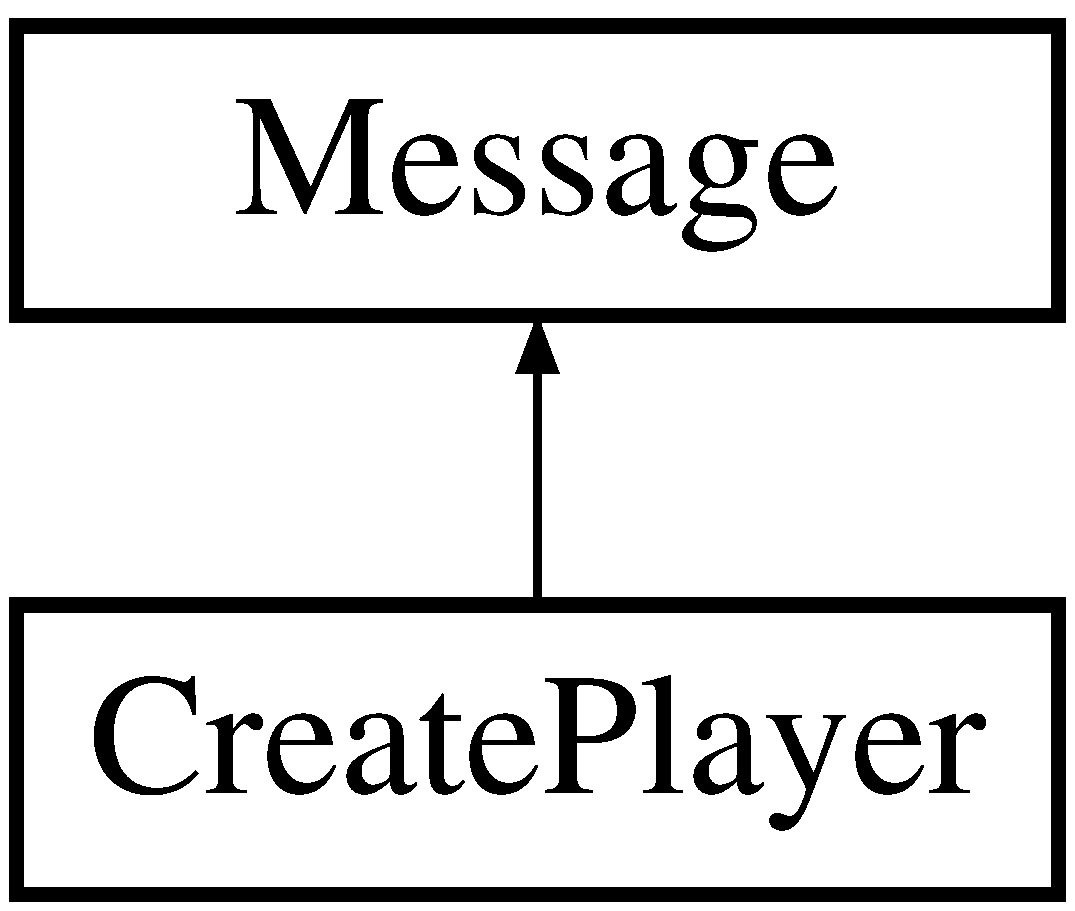
\includegraphics[height=2.000000cm]{class_create_player}
\end{center}
\end{figure}
\subsection*{Public Member Functions}
\begin{DoxyCompactItemize}
\item 
\hypertarget{class_create_player_a5467ecbd35d70d79efdb29585750ebdd}{{\bfseries Create\-Player} (const \hyperlink{class_create_player}{Create\-Player} \&from)}\label{class_create_player_a5467ecbd35d70d79efdb29585750ebdd}

\item 
\hypertarget{class_create_player_a6d76729d94045fa53266443aa470a0fa}{\hyperlink{class_create_player}{Create\-Player} \& {\bfseries operator=} (const \hyperlink{class_create_player}{Create\-Player} \&from)}\label{class_create_player_a6d76729d94045fa53266443aa470a0fa}

\item 
\hypertarget{class_create_player_ae9037e8587010e7098b08f04baddf82a}{const \\*
\-::google\-::protobuf\-::\-Unknown\-Field\-Set \& {\bfseries unknown\-\_\-fields} () const }\label{class_create_player_ae9037e8587010e7098b08f04baddf82a}

\item 
\hypertarget{class_create_player_ae68cce2fe165a57865c55ea1df283b1c}{inline\-::google\-::protobuf\-::\-Unknown\-Field\-Set $\ast$ {\bfseries mutable\-\_\-unknown\-\_\-fields} ()}\label{class_create_player_ae68cce2fe165a57865c55ea1df283b1c}

\item 
\hypertarget{class_create_player_a4e03e69e9f10d6a793e116e8234959cf}{void {\bfseries Swap} (\hyperlink{class_create_player}{Create\-Player} $\ast$other)}\label{class_create_player_a4e03e69e9f10d6a793e116e8234959cf}

\item 
\hypertarget{class_create_player_ac32d4379f1fb60282feb65513c673739}{\hyperlink{class_create_player}{Create\-Player} $\ast$ {\bfseries New} () const }\label{class_create_player_ac32d4379f1fb60282feb65513c673739}

\item 
\hypertarget{class_create_player_acce271bc0b594deb9186de689a991b5b}{\hyperlink{class_create_player}{Create\-Player} $\ast$ {\bfseries New} (\-::google\-::protobuf\-::\-Arena $\ast$arena) const }\label{class_create_player_acce271bc0b594deb9186de689a991b5b}

\item 
\hypertarget{class_create_player_afa1a1c65463f21a36c60c624a2830f8b}{void {\bfseries Copy\-From} (const \-::google\-::protobuf\-::\-Message \&from)}\label{class_create_player_afa1a1c65463f21a36c60c624a2830f8b}

\item 
\hypertarget{class_create_player_ac69c59b01e955b2f6b54b187d37645a4}{void {\bfseries Merge\-From} (const \-::google\-::protobuf\-::\-Message \&from)}\label{class_create_player_ac69c59b01e955b2f6b54b187d37645a4}

\item 
\hypertarget{class_create_player_a6a7ceed0bae191b7507404dee9440860}{void {\bfseries Copy\-From} (const \hyperlink{class_create_player}{Create\-Player} \&from)}\label{class_create_player_a6a7ceed0bae191b7507404dee9440860}

\item 
\hypertarget{class_create_player_a62af2ac4cd8c25d25fb40b24490dce71}{void {\bfseries Merge\-From} (const \hyperlink{class_create_player}{Create\-Player} \&from)}\label{class_create_player_a62af2ac4cd8c25d25fb40b24490dce71}

\item 
\hypertarget{class_create_player_a16a5331943d8f0cb80ea016c2f6536c1}{void {\bfseries Clear} ()}\label{class_create_player_a16a5331943d8f0cb80ea016c2f6536c1}

\item 
\hypertarget{class_create_player_aac130736c0a2910be7f7b502c41e1803}{bool {\bfseries Is\-Initialized} () const }\label{class_create_player_aac130736c0a2910be7f7b502c41e1803}

\item 
\hypertarget{class_create_player_a03f9cb31155e0379958b26d6ee0489d1}{int {\bfseries Byte\-Size} () const }\label{class_create_player_a03f9cb31155e0379958b26d6ee0489d1}

\item 
\hypertarget{class_create_player_ab0ef8132426cd05a7942ea70fdb3ef7b}{bool {\bfseries Merge\-Partial\-From\-Coded\-Stream} (\-::google\-::protobuf\-::io\-::\-Coded\-Input\-Stream $\ast$input)}\label{class_create_player_ab0ef8132426cd05a7942ea70fdb3ef7b}

\item 
\hypertarget{class_create_player_a9e670ed1b78c0db0c678bce985ca03e1}{void {\bfseries Serialize\-With\-Cached\-Sizes} (\-::google\-::protobuf\-::io\-::\-Coded\-Output\-Stream $\ast$output) const }\label{class_create_player_a9e670ed1b78c0db0c678bce985ca03e1}

\item 
\hypertarget{class_create_player_af968007dbfa9e09c137061676ff8013d}{\-::google\-::protobuf\-::uint8 $\ast$ {\bfseries Serialize\-With\-Cached\-Sizes\-To\-Array} (\-::google\-::protobuf\-::uint8 $\ast$output) const }\label{class_create_player_af968007dbfa9e09c137061676ff8013d}

\item 
\hypertarget{class_create_player_ab0f6a7f624e2a7f9228d9975338e43c7}{int {\bfseries Get\-Cached\-Size} () const }\label{class_create_player_ab0f6a7f624e2a7f9228d9975338e43c7}

\item 
\hypertarget{class_create_player_a11570983e86bd3a1633488d4e3a0f517}{\-::google\-::protobuf\-::\-Metadata {\bfseries Get\-Metadata} () const }\label{class_create_player_a11570983e86bd3a1633488d4e3a0f517}

\item 
\hypertarget{class_create_player_af2ffb8cd0a75402ad5fee111437d9a1a}{bool {\bfseries has\-\_\-player} () const }\label{class_create_player_af2ffb8cd0a75402ad5fee111437d9a1a}

\item 
\hypertarget{class_create_player_a4f321cb527a655d1552cbe4b1948ddaa}{void {\bfseries clear\-\_\-player} ()}\label{class_create_player_a4f321cb527a655d1552cbe4b1948ddaa}

\item 
\hypertarget{class_create_player_a83b1387aa31d0b45ac3869b751b622c2}{const \-::std\-::string \& {\bfseries player} () const }\label{class_create_player_a83b1387aa31d0b45ac3869b751b622c2}

\item 
\hypertarget{class_create_player_a2db7b5bdd9a904e95cf9f6e692629dcf}{void {\bfseries set\-\_\-player} (const \-::std\-::string \&value)}\label{class_create_player_a2db7b5bdd9a904e95cf9f6e692629dcf}

\item 
\hypertarget{class_create_player_a0b88b81aaae8fd710466fd0a01e6b822}{void {\bfseries set\-\_\-player} (const char $\ast$value)}\label{class_create_player_a0b88b81aaae8fd710466fd0a01e6b822}

\item 
\hypertarget{class_create_player_aefe31b783cb70940616878c601f36a45}{void {\bfseries set\-\_\-player} (const char $\ast$value, size\-\_\-t size)}\label{class_create_player_aefe31b783cb70940616878c601f36a45}

\item 
\hypertarget{class_create_player_a1a2f1ea62c2005e3a40e58a84970e86e}{inline\-::std\-::string $\ast$ {\bfseries mutable\-\_\-player} ()}\label{class_create_player_a1a2f1ea62c2005e3a40e58a84970e86e}

\item 
\hypertarget{class_create_player_a1b9edd8ec11c71202f139f21867d48f1}{inline\-::std\-::string $\ast$ {\bfseries release\-\_\-player} ()}\label{class_create_player_a1b9edd8ec11c71202f139f21867d48f1}

\item 
\hypertarget{class_create_player_ae7b000ed1c762919baee49272fe890f4}{void {\bfseries set\-\_\-allocated\-\_\-player} (\-::std\-::string $\ast$player)}\label{class_create_player_ae7b000ed1c762919baee49272fe890f4}

\end{DoxyCompactItemize}
\subsection*{Static Public Member Functions}
\begin{DoxyCompactItemize}
\item 
\hypertarget{class_create_player_aa432a2da91bb59e44581d02030991ae1}{static const \\*
\-::google\-::protobuf\-::\-Descriptor $\ast$ {\bfseries descriptor} ()}\label{class_create_player_aa432a2da91bb59e44581d02030991ae1}

\item 
\hypertarget{class_create_player_aeea9db2427ab00cdd0dbb69f8aa26fca}{static const \hyperlink{class_create_player}{Create\-Player} \& {\bfseries default\-\_\-instance} ()}\label{class_create_player_aeea9db2427ab00cdd0dbb69f8aa26fca}

\end{DoxyCompactItemize}
\subsection*{Static Public Attributes}
\begin{DoxyCompactItemize}
\item 
\hypertarget{class_create_player_a301c293ca078a99b8fe8aeaa5e269aa2}{static const int {\bfseries k\-Player\-Field\-Number} = 1}\label{class_create_player_a301c293ca078a99b8fe8aeaa5e269aa2}

\end{DoxyCompactItemize}
\subsection*{Friends}
\begin{DoxyCompactItemize}
\item 
\hypertarget{class_create_player_a508cc52b267f30a83163d9b681c4cdba}{void {\bfseries protobuf\-\_\-\-Add\-Desc\-\_\-\-Create\-Player\-\_\-2eproto} ()}\label{class_create_player_a508cc52b267f30a83163d9b681c4cdba}

\item 
\hypertarget{class_create_player_a41a443b4974448f74d433d838b28d2db}{void {\bfseries protobuf\-\_\-\-Assign\-Desc\-\_\-\-Create\-Player\-\_\-2eproto} ()}\label{class_create_player_a41a443b4974448f74d433d838b28d2db}

\item 
\hypertarget{class_create_player_acb5335721b54abf232629cbda4a21551}{void {\bfseries protobuf\-\_\-\-Shutdown\-File\-\_\-\-Create\-Player\-\_\-2eproto} ()}\label{class_create_player_acb5335721b54abf232629cbda4a21551}

\end{DoxyCompactItemize}


The documentation for this class was generated from the following files\-:\begin{DoxyCompactItemize}
\item 
protobufmessage/Create\-Player.\-pb.\-h\item 
protobufmessage/Create\-Player.\-pb.\-cc\end{DoxyCompactItemize}

\hypertarget{class_double_circular_list}{\section{Double\-Circular\-List$<$ E $>$ Class Template Reference}
\label{class_double_circular_list}\index{Double\-Circular\-List$<$ E $>$@{Double\-Circular\-List$<$ E $>$}}
}


Esta clase es una estructura de datos especificamente una lista doblemente enlazada circular que puede contener cualquier tipo de dato solamente definiciendolo mediante el template de esta clase. se puede agregar y borrar el dato.  




{\ttfamily \#include $<$Double\-Circular\-List.\-h$>$}

Inheritance diagram for Double\-Circular\-List$<$ E $>$\-:\begin{figure}[H]
\begin{center}
\leavevmode
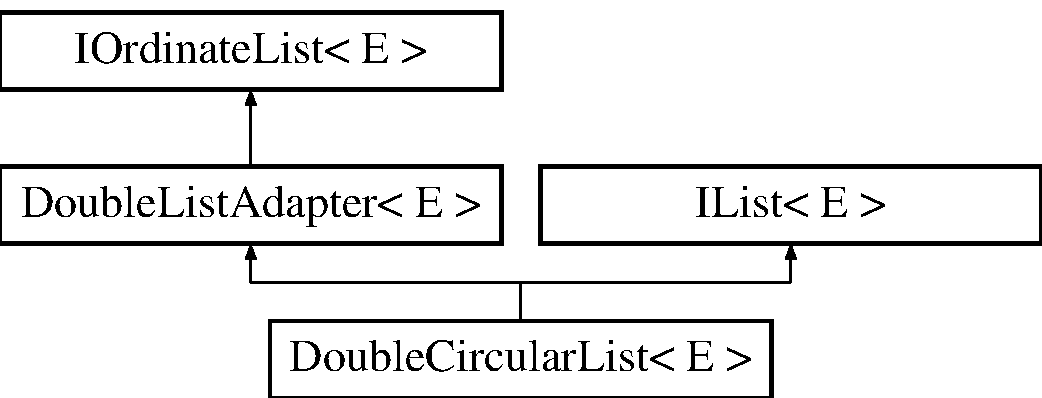
\includegraphics[height=3.000000cm]{class_double_circular_list}
\end{center}
\end{figure}
\subsection*{Public Member Functions}
\begin{DoxyCompactItemize}
\item 
\hyperlink{class_double_circular_list_a533876254e3c837d556542eda9968f8b}{Double\-Circular\-List} ()
\begin{DoxyCompactList}\small\item\em Es el constructor de la lista circular doble. \end{DoxyCompactList}\item 
void \hyperlink{class_double_circular_list_ade2ef68a86a8deef4cb43d38e031906b}{addi} (E)
\begin{DoxyCompactList}\small\item\em Agrega un elemento al principio de la lista. \end{DoxyCompactList}\item 
void \hyperlink{class_double_circular_list_a7691d38e77ea44d222c465f27e7d05b6}{add} (E)
\begin{DoxyCompactList}\small\item\em Agregar un elemento al final de la lista. \end{DoxyCompactList}\item 
bool \hyperlink{class_double_circular_list_a6d76f7045dd9997f55c6c2feb80678da}{add} (E, int)
\begin{DoxyCompactList}\small\item\em Agrega el elemento en el indice indicado. Si el indice es incorrecto no se agrega el elemento. \end{DoxyCompactList}\item 
bool \hyperlink{class_double_circular_list_ae7ed8b6714720cb7daafa639f232ecc3}{remove} (int)
\begin{DoxyCompactList}\small\item\em Remueve el dato en la posicion indicada por el parametro, en caso que el indice indicado sea incorrecto, osea que sea menor que cero o mayor o igual que el largo de la lista no alterara la lista. \end{DoxyCompactList}\item 
void \hyperlink{class_double_circular_list_a95e0f27bda1158233015ee3ff27b3ade}{set} (int, E)
\begin{DoxyCompactList}\small\item\em Setea el valor del dato que se encuentre en el indice citado con un nuevo valor. \end{DoxyCompactList}\item 
E \hyperlink{class_double_circular_list_aa00bc8fd524af1ba208f85d8816dec52}{get} (int)
\begin{DoxyCompactList}\small\item\em Obtiene un dato el la posicion indicada. En caso que el indice indicado sea incorrecto, osea que sea menor que cero o mayor o igual que el largo de la lista arrojara un error pues el dato esta fuera de los limites de la lista. \end{DoxyCompactList}\item 
\hyperlink{class_i_iterator}{I\-Iterator}$<$ E $>$ $\ast$ \hyperlink{class_double_circular_list_abba1430e956c7660a88f786bfd8d87ad}{get\-Iterator} ()
\begin{DoxyCompactList}\small\item\em Obtiene una instancia de un nuevo iterador de esta lista, y pueden obtenerse cuantas sean necesarias. pero es responsabilidad del programador eliminar mediante la palabra reservada delete. Ademas este puede ser un iterador inverso o normal, eso quiere decir que el iterador puede recorrer la lista al reves o al derecho respectivamente a los iteradores anteriormente citados. El tipo de iterador puede ser señalado con la funcion \hyperlink{class_double_circular_list_a77212c5d6ad148c99a06009a8c44128b}{Double\-Circular\-List\-::inverse\-Iteration(bool)}\end{DoxyCompactList}\item 
void \hyperlink{class_double_circular_list_a77212c5d6ad148c99a06009a8c44128b}{inverse\-Iteration} (bool)
\begin{DoxyCompactList}\small\item\em Decide si el iterador es inverso o normal. \end{DoxyCompactList}\item 
virtual \hyperlink{class_double_circular_list_a26dba8b85983742cfbf38886245fe2a4}{$\sim$\-Double\-Circular\-List} ()
\begin{DoxyCompactList}\small\item\em Es el destructor de la lista. \end{DoxyCompactList}\item 
\hyperlink{class_double_circular_list_a533876254e3c837d556542eda9968f8b}{Double\-Circular\-List} ()
\end{DoxyCompactItemize}
\subsection*{Protected Member Functions}
\begin{DoxyCompactItemize}
\item 
bool \hyperlink{class_double_circular_list_aee387acc4f53773302be4aa98bc779dc}{addi} (E p\-Data)
\begin{DoxyCompactList}\small\item\em Agrega un elemento al principio de la lista. \end{DoxyCompactList}\item 
bool \hyperlink{class_double_circular_list_a4a6ec7a7298470389b88b0c775a9bace}{addf} (E p\-Data)
\item 
bool \hyperlink{class_double_circular_list_aff5a0088509cc88dccfe31389d48f19e}{add\-First\-Data} (E p\-Data)
\item 
bool \hyperlink{class_double_circular_list_a1d2c6f1fec95c8d2887c54cb3fc3ff84}{removei} ()
\item 
bool \hyperlink{class_double_circular_list_a937da114318f91c6013dd4543636da9d}{removef} ()
\end{DoxyCompactItemize}
\subsection*{Additional Inherited Members}


\subsection{Detailed Description}
\subsubsection*{template$<$class E$>$class Double\-Circular\-List$<$ E $>$}

Esta clase es una estructura de datos especificamente una lista doblemente enlazada circular que puede contener cualquier tipo de dato solamente definiciendolo mediante el template de esta clase. se puede agregar y borrar el dato. 

\subsection{Constructor \& Destructor Documentation}
\hypertarget{class_double_circular_list_a533876254e3c837d556542eda9968f8b}{\index{Double\-Circular\-List@{Double\-Circular\-List}!Double\-Circular\-List@{Double\-Circular\-List}}
\index{Double\-Circular\-List@{Double\-Circular\-List}!DoubleCircularList@{Double\-Circular\-List}}
\subsubsection[{Double\-Circular\-List}]{\setlength{\rightskip}{0pt plus 5cm}template$<$class E $>$ {\bf Double\-Circular\-List}$<$ E $>$\-::{\bf Double\-Circular\-List} (
\begin{DoxyParamCaption}
{}
\end{DoxyParamCaption}
)}}\label{class_double_circular_list_a533876254e3c837d556542eda9968f8b}


Es el constructor de la lista circular doble. 

\hypertarget{class_double_circular_list_a26dba8b85983742cfbf38886245fe2a4}{\index{Double\-Circular\-List@{Double\-Circular\-List}!$\sim$\-Double\-Circular\-List@{$\sim$\-Double\-Circular\-List}}
\index{$\sim$\-Double\-Circular\-List@{$\sim$\-Double\-Circular\-List}!DoubleCircularList@{Double\-Circular\-List}}
\subsubsection[{$\sim$\-Double\-Circular\-List}]{\setlength{\rightskip}{0pt plus 5cm}template$<$class E $>$ {\bf Double\-Circular\-List}$<$ E $>$\-::$\sim${\bf Double\-Circular\-List} (
\begin{DoxyParamCaption}
{}
\end{DoxyParamCaption}
)\hspace{0.3cm}{\ttfamily [virtual]}}}\label{class_double_circular_list_a26dba8b85983742cfbf38886245fe2a4}


Es el destructor de la lista. 

\hypertarget{class_double_circular_list_a533876254e3c837d556542eda9968f8b}{\index{Double\-Circular\-List@{Double\-Circular\-List}!Double\-Circular\-List@{Double\-Circular\-List}}
\index{Double\-Circular\-List@{Double\-Circular\-List}!DoubleCircularList@{Double\-Circular\-List}}
\subsubsection[{Double\-Circular\-List}]{\setlength{\rightskip}{0pt plus 5cm}template$<$class E $>$ {\bf Double\-Circular\-List}$<$ E $>$\-::{\bf Double\-Circular\-List} (
\begin{DoxyParamCaption}
{}
\end{DoxyParamCaption}
)}}\label{class_double_circular_list_a533876254e3c837d556542eda9968f8b}


\subsection{Member Function Documentation}
\hypertarget{class_double_circular_list_a7691d38e77ea44d222c465f27e7d05b6}{\index{Double\-Circular\-List@{Double\-Circular\-List}!add@{add}}
\index{add@{add}!DoubleCircularList@{Double\-Circular\-List}}
\subsubsection[{add}]{\setlength{\rightskip}{0pt plus 5cm}template$<$class E $>$ void {\bf Double\-Circular\-List}$<$ E $>$\-::add (
\begin{DoxyParamCaption}
\item[{E}]{data}
\end{DoxyParamCaption}
)\hspace{0.3cm}{\ttfamily [virtual]}}}\label{class_double_circular_list_a7691d38e77ea44d222c465f27e7d05b6}


Agregar un elemento al final de la lista. 


\begin{DoxyParams}{Parameters}
{\em data} & el elemento a agregar \\
\hline
\end{DoxyParams}


Implements \hyperlink{class_i_list_a27500caa3d9da05aa6437d5ff56b09e2}{I\-List$<$ E $>$}.

\hypertarget{class_double_circular_list_a6d76f7045dd9997f55c6c2feb80678da}{\index{Double\-Circular\-List@{Double\-Circular\-List}!add@{add}}
\index{add@{add}!DoubleCircularList@{Double\-Circular\-List}}
\subsubsection[{add}]{\setlength{\rightskip}{0pt plus 5cm}template$<$class E $>$ bool {\bf Double\-Circular\-List}$<$ E $>$\-::add (
\begin{DoxyParamCaption}
\item[{E}]{data, }
\item[{int}]{index}
\end{DoxyParamCaption}
)\hspace{0.3cm}{\ttfamily [virtual]}}}\label{class_double_circular_list_a6d76f7045dd9997f55c6c2feb80678da}


Agrega el elemento en el indice indicado. Si el indice es incorrecto no se agrega el elemento. 


\begin{DoxyParams}{Parameters}
{\em data} & el elemento a agregar \\
\hline
{\em index} & el indice que indica el lugar donde se agragegara \\
\hline
\end{DoxyParams}
\begin{DoxyReturn}{Returns}
si el elemento se agrega retorna true, en caso contrario retorna false 
\end{DoxyReturn}


Implements \hyperlink{class_i_list_a70140dbc9de2b9f6e5ffd2212d5ea8b0}{I\-List$<$ E $>$}.

\hypertarget{class_double_circular_list_a4a6ec7a7298470389b88b0c775a9bace}{\index{Double\-Circular\-List@{Double\-Circular\-List}!addf@{addf}}
\index{addf@{addf}!DoubleCircularList@{Double\-Circular\-List}}
\subsubsection[{addf}]{\setlength{\rightskip}{0pt plus 5cm}template$<$class E $>$ bool {\bf Double\-Circular\-List}$<$ E $>$\-::addf (
\begin{DoxyParamCaption}
\item[{E}]{p\-Data}
\end{DoxyParamCaption}
)\hspace{0.3cm}{\ttfamily [protected]}, {\ttfamily [virtual]}}}\label{class_double_circular_list_a4a6ec7a7298470389b88b0c775a9bace}


Implements \hyperlink{class_double_list_adapter_adf4e6a8a4479d1fa0e692aea0d254c0f}{Double\-List\-Adapter$<$ E $>$}.

\hypertarget{class_double_circular_list_aff5a0088509cc88dccfe31389d48f19e}{\index{Double\-Circular\-List@{Double\-Circular\-List}!add\-First\-Data@{add\-First\-Data}}
\index{add\-First\-Data@{add\-First\-Data}!DoubleCircularList@{Double\-Circular\-List}}
\subsubsection[{add\-First\-Data}]{\setlength{\rightskip}{0pt plus 5cm}template$<$class E $>$ bool {\bf Double\-Circular\-List}$<$ E $>$\-::add\-First\-Data (
\begin{DoxyParamCaption}
\item[{E}]{p\-Data}
\end{DoxyParamCaption}
)\hspace{0.3cm}{\ttfamily [protected]}, {\ttfamily [virtual]}}}\label{class_double_circular_list_aff5a0088509cc88dccfe31389d48f19e}


Implements \hyperlink{class_double_list_adapter_a024ff60d5cb3e11ff5be795f48deaac0}{Double\-List\-Adapter$<$ E $>$}.

\hypertarget{class_double_circular_list_aee387acc4f53773302be4aa98bc779dc}{\index{Double\-Circular\-List@{Double\-Circular\-List}!addi@{addi}}
\index{addi@{addi}!DoubleCircularList@{Double\-Circular\-List}}
\subsubsection[{addi}]{\setlength{\rightskip}{0pt plus 5cm}template$<$class E $>$ bool {\bf Double\-Circular\-List}$<$ E $>$\-::addi (
\begin{DoxyParamCaption}
\item[{E}]{}
\end{DoxyParamCaption}
)\hspace{0.3cm}{\ttfamily [protected]}, {\ttfamily [virtual]}}}\label{class_double_circular_list_aee387acc4f53773302be4aa98bc779dc}


Agrega un elemento al principio de la lista. 


\begin{DoxyParams}{Parameters}
{\em data} & el elemento a agregar \\
\hline
\end{DoxyParams}


Implements \hyperlink{class_i_list_af202dc9e748ee32238d80e57dfbcae20}{I\-List$<$ E $>$}.

\hypertarget{class_double_circular_list_ade2ef68a86a8deef4cb43d38e031906b}{\index{Double\-Circular\-List@{Double\-Circular\-List}!addi@{addi}}
\index{addi@{addi}!DoubleCircularList@{Double\-Circular\-List}}
\subsubsection[{addi}]{\setlength{\rightskip}{0pt plus 5cm}template$<$class E $>$ bool {\bf Double\-Circular\-List}$<$ E $>$\-::addi (
\begin{DoxyParamCaption}
\item[{E}]{data}
\end{DoxyParamCaption}
)\hspace{0.3cm}{\ttfamily [virtual]}}}\label{class_double_circular_list_ade2ef68a86a8deef4cb43d38e031906b}


Agrega un elemento al principio de la lista. 


\begin{DoxyParams}{Parameters}
{\em data} & el elemento a agregar \\
\hline
\end{DoxyParams}


Implements \hyperlink{class_i_list_af202dc9e748ee32238d80e57dfbcae20}{I\-List$<$ E $>$}.

\hypertarget{class_double_circular_list_aa00bc8fd524af1ba208f85d8816dec52}{\index{Double\-Circular\-List@{Double\-Circular\-List}!get@{get}}
\index{get@{get}!DoubleCircularList@{Double\-Circular\-List}}
\subsubsection[{get}]{\setlength{\rightskip}{0pt plus 5cm}template$<$class E $>$ E {\bf Double\-Circular\-List}$<$ E $>$\-::get (
\begin{DoxyParamCaption}
\item[{int}]{index}
\end{DoxyParamCaption}
)\hspace{0.3cm}{\ttfamily [virtual]}}}\label{class_double_circular_list_aa00bc8fd524af1ba208f85d8816dec52}


Obtiene un dato el la posicion indicada. En caso que el indice indicado sea incorrecto, osea que sea menor que cero o mayor o igual que el largo de la lista arrojara un error pues el dato esta fuera de los limites de la lista. 


\begin{DoxyParams}{Parameters}
{\em index} & el indice indicado \\
\hline
\end{DoxyParams}
\begin{DoxyReturn}{Returns}
data el dato buscado por el indice indicado 
\end{DoxyReturn}

\begin{DoxyExceptions}{Exceptions}
{\em indexoutbounds} & fuera de rango si index es menor que cero o index es mayor o igual que el largo de la lista \\
\hline
\end{DoxyExceptions}


Implements \hyperlink{class_i_list_a60570f7ee0e7474d01b2f364bad996a0}{I\-List$<$ E $>$}.

\hypertarget{class_double_circular_list_abba1430e956c7660a88f786bfd8d87ad}{\index{Double\-Circular\-List@{Double\-Circular\-List}!get\-Iterator@{get\-Iterator}}
\index{get\-Iterator@{get\-Iterator}!DoubleCircularList@{Double\-Circular\-List}}
\subsubsection[{get\-Iterator}]{\setlength{\rightskip}{0pt plus 5cm}template$<$class E $>$ {\bf I\-Iterator}$<$ E $>$ $\ast$ {\bf Double\-Circular\-List}$<$ E $>$\-::get\-Iterator (
\begin{DoxyParamCaption}
{}
\end{DoxyParamCaption}
)\hspace{0.3cm}{\ttfamily [virtual]}}}\label{class_double_circular_list_abba1430e956c7660a88f786bfd8d87ad}


Obtiene una instancia de un nuevo iterador de esta lista, y pueden obtenerse cuantas sean necesarias. pero es responsabilidad del programador eliminar mediante la palabra reservada delete. Ademas este puede ser un iterador inverso o normal, eso quiere decir que el iterador puede recorrer la lista al reves o al derecho respectivamente a los iteradores anteriormente citados. El tipo de iterador puede ser señalado con la funcion \hyperlink{class_double_circular_list_a77212c5d6ad148c99a06009a8c44128b}{Double\-Circular\-List\-::inverse\-Iteration(bool)}

\begin{DoxyReturn}{Returns}
I\-Iterator$<$\-E$>$ un puntero del iterador indicado 
\end{DoxyReturn}


Implements \hyperlink{class_i_list_a997815664cc6b20eb5dfa9968251d2cd}{I\-List$<$ E $>$}.

\hypertarget{class_double_circular_list_a77212c5d6ad148c99a06009a8c44128b}{\index{Double\-Circular\-List@{Double\-Circular\-List}!inverse\-Iteration@{inverse\-Iteration}}
\index{inverse\-Iteration@{inverse\-Iteration}!DoubleCircularList@{Double\-Circular\-List}}
\subsubsection[{inverse\-Iteration}]{\setlength{\rightskip}{0pt plus 5cm}template$<$class E $>$ void {\bf Double\-Circular\-List}$<$ E $>$\-::inverse\-Iteration (
\begin{DoxyParamCaption}
\item[{bool}]{inverse}
\end{DoxyParamCaption}
)}}\label{class_double_circular_list_a77212c5d6ad148c99a06009a8c44128b}


Decide si el iterador es inverso o normal. 


\begin{DoxyParams}{Parameters}
{\em si} & es true el iterador sera inverso, false es un iterador normal \\
\hline
\end{DoxyParams}
\hypertarget{class_double_circular_list_ae7ed8b6714720cb7daafa639f232ecc3}{\index{Double\-Circular\-List@{Double\-Circular\-List}!remove@{remove}}
\index{remove@{remove}!DoubleCircularList@{Double\-Circular\-List}}
\subsubsection[{remove}]{\setlength{\rightskip}{0pt plus 5cm}template$<$class E $>$ bool {\bf Double\-Circular\-List}$<$ E $>$\-::remove (
\begin{DoxyParamCaption}
\item[{int}]{index}
\end{DoxyParamCaption}
)\hspace{0.3cm}{\ttfamily [virtual]}}}\label{class_double_circular_list_ae7ed8b6714720cb7daafa639f232ecc3}


Remueve el dato en la posicion indicada por el parametro, en caso que el indice indicado sea incorrecto, osea que sea menor que cero o mayor o igual que el largo de la lista no alterara la lista. 


\begin{DoxyParams}{Parameters}
{\em index} & la posicion indicada del objeto a borrar \\
\hline
\end{DoxyParams}
\begin{DoxyReturn}{Returns}
true si borra algo, false si el indice indicado es incorrecto 
\end{DoxyReturn}


Implements \hyperlink{class_i_list_a9bf7d737252dfbd4c9a5d7be36ea4231}{I\-List$<$ E $>$}.

\hypertarget{class_double_circular_list_a937da114318f91c6013dd4543636da9d}{\index{Double\-Circular\-List@{Double\-Circular\-List}!removef@{removef}}
\index{removef@{removef}!DoubleCircularList@{Double\-Circular\-List}}
\subsubsection[{removef}]{\setlength{\rightskip}{0pt plus 5cm}template$<$class E $>$ bool {\bf Double\-Circular\-List}$<$ E $>$\-::removef (
\begin{DoxyParamCaption}
{}
\end{DoxyParamCaption}
)\hspace{0.3cm}{\ttfamily [protected]}, {\ttfamily [virtual]}}}\label{class_double_circular_list_a937da114318f91c6013dd4543636da9d}


Implements \hyperlink{class_double_list_adapter_a1f069987bb3e8abcccf24659474960c3}{Double\-List\-Adapter$<$ E $>$}.

\hypertarget{class_double_circular_list_a1d2c6f1fec95c8d2887c54cb3fc3ff84}{\index{Double\-Circular\-List@{Double\-Circular\-List}!removei@{removei}}
\index{removei@{removei}!DoubleCircularList@{Double\-Circular\-List}}
\subsubsection[{removei}]{\setlength{\rightskip}{0pt plus 5cm}template$<$class E $>$ bool {\bf Double\-Circular\-List}$<$ E $>$\-::removei (
\begin{DoxyParamCaption}
{}
\end{DoxyParamCaption}
)\hspace{0.3cm}{\ttfamily [protected]}, {\ttfamily [virtual]}}}\label{class_double_circular_list_a1d2c6f1fec95c8d2887c54cb3fc3ff84}


Implements \hyperlink{class_double_list_adapter_a710e75ff353e5e94ae1fb9eadc0b582b}{Double\-List\-Adapter$<$ E $>$}.

\hypertarget{class_double_circular_list_a95e0f27bda1158233015ee3ff27b3ade}{\index{Double\-Circular\-List@{Double\-Circular\-List}!set@{set}}
\index{set@{set}!DoubleCircularList@{Double\-Circular\-List}}
\subsubsection[{set}]{\setlength{\rightskip}{0pt plus 5cm}template$<$class E $>$ void {\bf Double\-Circular\-List}$<$ E $>$\-::set (
\begin{DoxyParamCaption}
\item[{int}]{index, }
\item[{E}]{data}
\end{DoxyParamCaption}
)\hspace{0.3cm}{\ttfamily [virtual]}}}\label{class_double_circular_list_a95e0f27bda1158233015ee3ff27b3ade}


Setea el valor del dato que se encuentre en el indice citado con un nuevo valor. 


\begin{DoxyParams}{Parameters}
{\em index} & el indice en el que se encuetra el dato \\
\hline
{\em data} & el dato por el que se cambiara \\
\hline
\end{DoxyParams}


Implements \hyperlink{class_i_list_a119ed658d2804aec0b9fef9325c03073}{I\-List$<$ E $>$}.



The documentation for this class was generated from the following file\-:\begin{DoxyCompactItemize}
\item 
list/\hyperlink{_double_circular_list_8h}{Double\-Circular\-List.\-h}\end{DoxyCompactItemize}

\hypertarget{class_double_iterator}{\section{Double\-Iterator$<$ E $>$ Class Template Reference}
\label{class_double_iterator}\index{Double\-Iterator$<$ E $>$@{Double\-Iterator$<$ E $>$}}
}


Esta clase es un iterador de las listas doblemente enlazadas, ademas la actualizacion de la lista N\-O actualiza el iterador, por lo que el iterador es momentaneo. Es similar a una fotografia de una lista que no ha sido alterada si la lista se altera usando un iterador puede que el iterador falle. Por lo que es recomendable que la lista no se actualice mientras se usa un iterador.  




{\ttfamily \#include $<$Double\-Iterator.\-h$>$}

Inheritance diagram for Double\-Iterator$<$ E $>$\-:\begin{figure}[H]
\begin{center}
\leavevmode
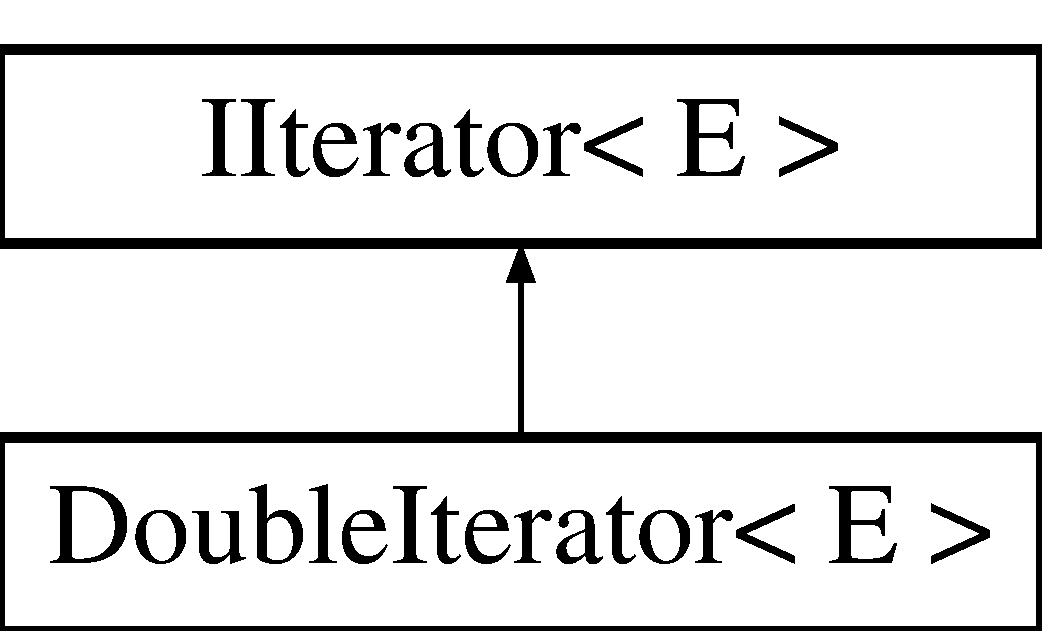
\includegraphics[height=2.000000cm]{class_double_iterator}
\end{center}
\end{figure}
\subsection*{Public Member Functions}
\begin{DoxyCompactItemize}
\item 
\hyperlink{class_double_iterator_a5b45a91dc363462fddcb4965e226e2fc}{Double\-Iterator} (\hyperlink{class_double_node}{Double\-Node}$<$ E $>$ $\ast$, \hyperlink{class_double_node}{Double\-Node}$<$ E $>$ $\ast$)
\begin{DoxyCompactList}\small\item\em Metodo constructor. \end{DoxyCompactList}\item 
E \hyperlink{class_double_iterator_aaaa1b361a61339bfee3bf86f3f67b198}{get\-Next} ()
\begin{DoxyCompactList}\small\item\em Obtiene el dato actual y actualiza al nodo siguiente. \end{DoxyCompactList}\item 
E \hyperlink{class_double_iterator_a756bb08f5352e270e08b72339c32e2be}{get\-Current} () const 
\begin{DoxyCompactList}\small\item\em Obtiene el dato actual. \end{DoxyCompactList}\item 
bool \hyperlink{class_double_iterator_adb5ef4c66649e0a4ce18e38cd85904ed}{has\-Next} () const 
\begin{DoxyCompactList}\small\item\em Verifica si tiene siguiente. \end{DoxyCompactList}\end{DoxyCompactItemize}
\subsection*{Friends}
\begin{DoxyCompactItemize}
\item 
\hypertarget{class_double_iterator_ad435a9844a002995926acf522128f7a8}{{\footnotesize template$<$class T $>$ }\\class {\bfseries Double\-List}}\label{class_double_iterator_ad435a9844a002995926acf522128f7a8}

\end{DoxyCompactItemize}


\subsection{Detailed Description}
\subsubsection*{template$<$class E$>$class Double\-Iterator$<$ E $>$}

Esta clase es un iterador de las listas doblemente enlazadas, ademas la actualizacion de la lista N\-O actualiza el iterador, por lo que el iterador es momentaneo. Es similar a una fotografia de una lista que no ha sido alterada si la lista se altera usando un iterador puede que el iterador falle. Por lo que es recomendable que la lista no se actualice mientras se usa un iterador. 

\subsection{Constructor \& Destructor Documentation}
\hypertarget{class_double_iterator_a5b45a91dc363462fddcb4965e226e2fc}{\index{Double\-Iterator@{Double\-Iterator}!Double\-Iterator@{Double\-Iterator}}
\index{Double\-Iterator@{Double\-Iterator}!DoubleIterator@{Double\-Iterator}}
\subsubsection[{Double\-Iterator}]{\setlength{\rightskip}{0pt plus 5cm}template$<$class E $>$ {\bf Double\-Iterator}$<$ E $>$\-::{\bf Double\-Iterator} (
\begin{DoxyParamCaption}
\item[{{\bf Double\-Node}$<$ E $>$ $\ast$}]{head, }
\item[{{\bf Double\-Node}$<$ E $>$ $\ast$}]{tail}
\end{DoxyParamCaption}
)}}\label{class_double_iterator_a5b45a91dc363462fddcb4965e226e2fc}


Metodo constructor. 


\begin{DoxyParams}{Parameters}
{\em head} & es la cabeza por donde se iniciara la iteracion \\
\hline
{\em tail} & es la cola el ultimo elemento de la iteracion \\
\hline
\end{DoxyParams}


\subsection{Member Function Documentation}
\hypertarget{class_double_iterator_a756bb08f5352e270e08b72339c32e2be}{\index{Double\-Iterator@{Double\-Iterator}!get\-Current@{get\-Current}}
\index{get\-Current@{get\-Current}!DoubleIterator@{Double\-Iterator}}
\subsubsection[{get\-Current}]{\setlength{\rightskip}{0pt plus 5cm}template$<$class E $>$ E {\bf Double\-Iterator}$<$ E $>$\-::get\-Current (
\begin{DoxyParamCaption}
{}
\end{DoxyParamCaption}
) const\hspace{0.3cm}{\ttfamily [virtual]}}}\label{class_double_iterator_a756bb08f5352e270e08b72339c32e2be}


Obtiene el dato actual. 

\begin{DoxyReturn}{Returns}
E el dato actual 
\end{DoxyReturn}

\begin{DoxyExceptions}{Exceptions}
{\em donthavenext} & si el dato actual es nulo \\
\hline
\end{DoxyExceptions}


Implements \hyperlink{class_i_iterator_a50f55ce1381378aad2c93f16c9b60822}{I\-Iterator$<$ E $>$}.

\hypertarget{class_double_iterator_aaaa1b361a61339bfee3bf86f3f67b198}{\index{Double\-Iterator@{Double\-Iterator}!get\-Next@{get\-Next}}
\index{get\-Next@{get\-Next}!DoubleIterator@{Double\-Iterator}}
\subsubsection[{get\-Next}]{\setlength{\rightskip}{0pt plus 5cm}template$<$class E $>$ E {\bf Double\-Iterator}$<$ E $>$\-::get\-Next (
\begin{DoxyParamCaption}
{}
\end{DoxyParamCaption}
)\hspace{0.3cm}{\ttfamily [virtual]}}}\label{class_double_iterator_aaaa1b361a61339bfee3bf86f3f67b198}


Obtiene el dato actual y actualiza al nodo siguiente. 

\begin{DoxyReturn}{Returns}
E el dato actual 
\end{DoxyReturn}

\begin{DoxyExceptions}{Exceptions}
{\em donthavenext} & si el dato actual es nulo \\
\hline
\end{DoxyExceptions}


Implements \hyperlink{class_i_iterator_ab1b13434e4fac20c74262dee51d1e870}{I\-Iterator$<$ E $>$}.

\hypertarget{class_double_iterator_adb5ef4c66649e0a4ce18e38cd85904ed}{\index{Double\-Iterator@{Double\-Iterator}!has\-Next@{has\-Next}}
\index{has\-Next@{has\-Next}!DoubleIterator@{Double\-Iterator}}
\subsubsection[{has\-Next}]{\setlength{\rightskip}{0pt plus 5cm}template$<$class E $>$ bool {\bf Double\-Iterator}$<$ E $>$\-::has\-Next (
\begin{DoxyParamCaption}
{}
\end{DoxyParamCaption}
) const\hspace{0.3cm}{\ttfamily [virtual]}}}\label{class_double_iterator_adb5ef4c66649e0a4ce18e38cd85904ed}


Verifica si tiene siguiente. 

\begin{DoxyReturn}{Returns}
true si tiene siguiente, false si no lo tiene 
\end{DoxyReturn}

\begin{DoxyExceptions}{Exceptions}
{\em donthavenext} & si el dato actual es nulo \\
\hline
\end{DoxyExceptions}


Implements \hyperlink{class_i_iterator_a8a73f0fb41a66fe98e5e636378759196}{I\-Iterator$<$ E $>$}.



The documentation for this class was generated from the following file\-:\begin{DoxyCompactItemize}
\item 
list/Double\-Iterator.\-h\end{DoxyCompactItemize}

\hypertarget{class_double_list}{\section{Double\-List$<$ E $>$ Class Template Reference}
\label{class_double_list}\index{Double\-List$<$ E $>$@{Double\-List$<$ E $>$}}
}


Esta clase es una estructura de datos especificamente una lista doblemente enlazada que puede contener cualquier tipo de dato solamente definiciendolo mediante el template de esta clase. se puede agregar y borrar el dato.  




{\ttfamily \#include $<$Double\-List.\-h$>$}

Inheritance diagram for Double\-List$<$ E $>$\-:\begin{figure}[H]
\begin{center}
\leavevmode
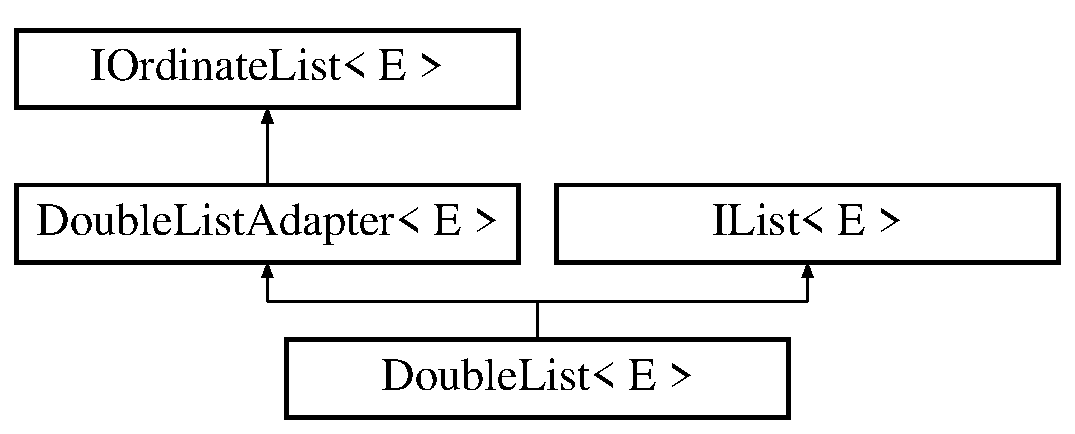
\includegraphics[height=3.000000cm]{class_double_list}
\end{center}
\end{figure}
\subsection*{Public Member Functions}
\begin{DoxyCompactItemize}
\item 
\hypertarget{class_double_list_ab54db9c718c7188f9413ef2b9982dd43}{\hyperlink{class_double_list_ab54db9c718c7188f9413ef2b9982dd43}{Double\-List} ()}\label{class_double_list_ab54db9c718c7188f9413ef2b9982dd43}

\begin{DoxyCompactList}\small\item\em Es el constructor de la lista doble. \end{DoxyCompactList}\item 
void \hyperlink{class_double_list_a621684e61b8d9d41cd107174d9877b1e}{addi} (E)
\begin{DoxyCompactList}\small\item\em Agrega un elemento al principio de la lista. \end{DoxyCompactList}\item 
void \hyperlink{class_double_list_adb96e6908d3d564722225b848350aa82}{add} (E)
\begin{DoxyCompactList}\small\item\em Agregar un elemento al final de la lista. \end{DoxyCompactList}\item 
bool \hyperlink{class_double_list_a84e3bb8be7d67b43dd3b63d5a47f80ed}{add} (E, int)
\begin{DoxyCompactList}\small\item\em Agrega el elemento en el indice indicado. Si el indice es incorrecto no se agrega el elemento. \end{DoxyCompactList}\item 
bool \hyperlink{class_double_list_a844c2c4c3b8260bd58ab94307359fb62}{remove} (int)
\begin{DoxyCompactList}\small\item\em Remueve el dato en la posicion indicada por el parametro, en caso que el indice indicado sea incorrecto, osea que sea menor que cero o mayor o igual que el largo de la lista no alterara la lista. \end{DoxyCompactList}\item 
void \hyperlink{class_double_list_a3c95ac3c3190b347c4a343776264bf67}{set} (int, E)
\begin{DoxyCompactList}\small\item\em Setea el valor del dato que se encuentre en el indice citado con un nuevo valor. \end{DoxyCompactList}\item 
E \hyperlink{class_double_list_a230a8c9c574abe9c72f8daae35127d9c}{get} (int)
\begin{DoxyCompactList}\small\item\em Obtiene un dato el la posicion indicada. En caso que el indice indicado sea incorrecto, osea que sea menor que cero o mayor o igual que el largo de la lista arrojara un error pues el dato esta fuera de los limites de la lista. \end{DoxyCompactList}\item 
\hyperlink{class_i_iterator}{I\-Iterator}$<$ E $>$ $\ast$ \hyperlink{class_double_list_aa14e383a97e054016a6c5178165b20df}{get\-Iterator} ()
\begin{DoxyCompactList}\small\item\em Obtiene una instancia de un nuevo iterador de esta lista, y pueden obtenerse cuantas sean necesarias. pero es responsabilidad del programador eliminar mediante la palabra reservada delete. Ademas este puede ser un iterador inverso o normal, eso quiere decir que el iterador puede recorrer la lista al reves o al derecho respectivamente a los iteradores anteriormente citados. El tipo de iterador puede ser señalado con la funcion \hyperlink{class_double_circular_list_a77212c5d6ad148c99a06009a8c44128b}{Double\-Circular\-List\-::inverse\-Iteration(bool)}\end{DoxyCompactList}\item 
void \hyperlink{class_double_list_a94d1ad5299452ea46839ba350ca501d1}{inverse\-Iteration} (bool)
\begin{DoxyCompactList}\small\item\em Decide si el iterador es inverso o normal. \end{DoxyCompactList}\item 
\hypertarget{class_double_list_a11ce233388fea7a5722a7d57cea400a3}{virtual \hyperlink{class_double_list_a11ce233388fea7a5722a7d57cea400a3}{$\sim$\-Double\-List} ()}\label{class_double_list_a11ce233388fea7a5722a7d57cea400a3}

\begin{DoxyCompactList}\small\item\em Es el destructor de la lista. \end{DoxyCompactList}\end{DoxyCompactItemize}
\subsection*{Protected Member Functions}
\begin{DoxyCompactItemize}
\item 
bool \hyperlink{class_double_list_a01623cc4b04d94c655de62ae373963b2}{addi} (E p\-Data)
\begin{DoxyCompactList}\small\item\em Agrega un elemento al principio de la lista. \end{DoxyCompactList}\item 
\hypertarget{class_double_list_a495cbf66dc7f7523e15405b762cc616d}{bool {\bfseries addf} (E p\-Data)}\label{class_double_list_a495cbf66dc7f7523e15405b762cc616d}

\item 
\hypertarget{class_double_list_a4d72bc061da9183185b9ae1896b2767b}{bool {\bfseries add\-First\-Data} (E p\-Data)}\label{class_double_list_a4d72bc061da9183185b9ae1896b2767b}

\item 
\hypertarget{class_double_list_a074473aaac863a9e00ec34c2316a2d9e}{bool {\bfseries removei} ()}\label{class_double_list_a074473aaac863a9e00ec34c2316a2d9e}

\item 
\hypertarget{class_double_list_a0cd7c06fa533e3f800778920346b8a7b}{bool {\bfseries removef} ()}\label{class_double_list_a0cd7c06fa533e3f800778920346b8a7b}

\end{DoxyCompactItemize}
\subsection*{Additional Inherited Members}


\subsection{Detailed Description}
\subsubsection*{template$<$class E$>$class Double\-List$<$ E $>$}

Esta clase es una estructura de datos especificamente una lista doblemente enlazada que puede contener cualquier tipo de dato solamente definiciendolo mediante el template de esta clase. se puede agregar y borrar el dato. 

\subsection{Member Function Documentation}
\hypertarget{class_double_list_adb96e6908d3d564722225b848350aa82}{\index{Double\-List@{Double\-List}!add@{add}}
\index{add@{add}!DoubleList@{Double\-List}}
\subsubsection[{add}]{\setlength{\rightskip}{0pt plus 5cm}template$<$class E $>$ void {\bf Double\-List}$<$ E $>$\-::add (
\begin{DoxyParamCaption}
\item[{E}]{data}
\end{DoxyParamCaption}
)\hspace{0.3cm}{\ttfamily [virtual]}}}\label{class_double_list_adb96e6908d3d564722225b848350aa82}


Agregar un elemento al final de la lista. 


\begin{DoxyParams}{Parameters}
{\em data} & el elemento a agregar \\
\hline
\end{DoxyParams}


Implements \hyperlink{class_i_list_a27500caa3d9da05aa6437d5ff56b09e2}{I\-List$<$ E $>$}.

\hypertarget{class_double_list_a84e3bb8be7d67b43dd3b63d5a47f80ed}{\index{Double\-List@{Double\-List}!add@{add}}
\index{add@{add}!DoubleList@{Double\-List}}
\subsubsection[{add}]{\setlength{\rightskip}{0pt plus 5cm}template$<$class E $>$ bool {\bf Double\-List}$<$ E $>$\-::add (
\begin{DoxyParamCaption}
\item[{E}]{data, }
\item[{int}]{index}
\end{DoxyParamCaption}
)\hspace{0.3cm}{\ttfamily [virtual]}}}\label{class_double_list_a84e3bb8be7d67b43dd3b63d5a47f80ed}


Agrega el elemento en el indice indicado. Si el indice es incorrecto no se agrega el elemento. 


\begin{DoxyParams}{Parameters}
{\em data} & el elemento a agregar \\
\hline
{\em index} & el indice que indica el lugar donde se agragegara \\
\hline
\end{DoxyParams}
\begin{DoxyReturn}{Returns}
si el elemento se agrega retorna true, en caso contrario retorna false 
\end{DoxyReturn}


Implements \hyperlink{class_i_list_a70140dbc9de2b9f6e5ffd2212d5ea8b0}{I\-List$<$ E $>$}.

\hypertarget{class_double_list_a01623cc4b04d94c655de62ae373963b2}{\index{Double\-List@{Double\-List}!addi@{addi}}
\index{addi@{addi}!DoubleList@{Double\-List}}
\subsubsection[{addi}]{\setlength{\rightskip}{0pt plus 5cm}template$<$class E $>$ bool {\bf Double\-List}$<$ E $>$\-::addi (
\begin{DoxyParamCaption}
\item[{E}]{}
\end{DoxyParamCaption}
)\hspace{0.3cm}{\ttfamily [protected]}, {\ttfamily [virtual]}}}\label{class_double_list_a01623cc4b04d94c655de62ae373963b2}


Agrega un elemento al principio de la lista. 


\begin{DoxyParams}{Parameters}
{\em data} & el elemento a agregar \\
\hline
\end{DoxyParams}


Implements \hyperlink{class_i_list_af202dc9e748ee32238d80e57dfbcae20}{I\-List$<$ E $>$}.

\hypertarget{class_double_list_a621684e61b8d9d41cd107174d9877b1e}{\index{Double\-List@{Double\-List}!addi@{addi}}
\index{addi@{addi}!DoubleList@{Double\-List}}
\subsubsection[{addi}]{\setlength{\rightskip}{0pt plus 5cm}template$<$class E $>$ bool {\bf Double\-List}$<$ E $>$\-::addi (
\begin{DoxyParamCaption}
\item[{E}]{data}
\end{DoxyParamCaption}
)\hspace{0.3cm}{\ttfamily [virtual]}}}\label{class_double_list_a621684e61b8d9d41cd107174d9877b1e}


Agrega un elemento al principio de la lista. 


\begin{DoxyParams}{Parameters}
{\em data} & el elemento a agregar \\
\hline
\end{DoxyParams}


Implements \hyperlink{class_i_list_af202dc9e748ee32238d80e57dfbcae20}{I\-List$<$ E $>$}.

\hypertarget{class_double_list_a230a8c9c574abe9c72f8daae35127d9c}{\index{Double\-List@{Double\-List}!get@{get}}
\index{get@{get}!DoubleList@{Double\-List}}
\subsubsection[{get}]{\setlength{\rightskip}{0pt plus 5cm}template$<$class E $>$ E {\bf Double\-List}$<$ E $>$\-::get (
\begin{DoxyParamCaption}
\item[{int}]{index}
\end{DoxyParamCaption}
)\hspace{0.3cm}{\ttfamily [virtual]}}}\label{class_double_list_a230a8c9c574abe9c72f8daae35127d9c}


Obtiene un dato el la posicion indicada. En caso que el indice indicado sea incorrecto, osea que sea menor que cero o mayor o igual que el largo de la lista arrojara un error pues el dato esta fuera de los limites de la lista. 


\begin{DoxyParams}{Parameters}
{\em index} & el indice indicado \\
\hline
\end{DoxyParams}
\begin{DoxyReturn}{Returns}
data el dato buscado por el indice indicado 
\end{DoxyReturn}

\begin{DoxyExceptions}{Exceptions}
{\em indexoutbounds} & fuera de rango si index es menor que cero o index es mayor o igual que el largo de la lista \\
\hline
\end{DoxyExceptions}


Implements \hyperlink{class_i_list_a60570f7ee0e7474d01b2f364bad996a0}{I\-List$<$ E $>$}.

\hypertarget{class_double_list_aa14e383a97e054016a6c5178165b20df}{\index{Double\-List@{Double\-List}!get\-Iterator@{get\-Iterator}}
\index{get\-Iterator@{get\-Iterator}!DoubleList@{Double\-List}}
\subsubsection[{get\-Iterator}]{\setlength{\rightskip}{0pt plus 5cm}template$<$class E $>$ {\bf I\-Iterator}$<$ E $>$ $\ast$ {\bf Double\-List}$<$ E $>$\-::get\-Iterator (
\begin{DoxyParamCaption}
{}
\end{DoxyParamCaption}
)\hspace{0.3cm}{\ttfamily [virtual]}}}\label{class_double_list_aa14e383a97e054016a6c5178165b20df}


Obtiene una instancia de un nuevo iterador de esta lista, y pueden obtenerse cuantas sean necesarias. pero es responsabilidad del programador eliminar mediante la palabra reservada delete. Ademas este puede ser un iterador inverso o normal, eso quiere decir que el iterador puede recorrer la lista al reves o al derecho respectivamente a los iteradores anteriormente citados. El tipo de iterador puede ser señalado con la funcion \hyperlink{class_double_circular_list_a77212c5d6ad148c99a06009a8c44128b}{Double\-Circular\-List\-::inverse\-Iteration(bool)}

\begin{DoxyReturn}{Returns}
I\-Iterator$<$\-E$>$ un puntero del iterador indicado 
\end{DoxyReturn}


Implements \hyperlink{class_i_list_a997815664cc6b20eb5dfa9968251d2cd}{I\-List$<$ E $>$}.

\hypertarget{class_double_list_a94d1ad5299452ea46839ba350ca501d1}{\index{Double\-List@{Double\-List}!inverse\-Iteration@{inverse\-Iteration}}
\index{inverse\-Iteration@{inverse\-Iteration}!DoubleList@{Double\-List}}
\subsubsection[{inverse\-Iteration}]{\setlength{\rightskip}{0pt plus 5cm}template$<$class E $>$ void {\bf Double\-List}$<$ E $>$\-::inverse\-Iteration (
\begin{DoxyParamCaption}
\item[{bool}]{inverse}
\end{DoxyParamCaption}
)}}\label{class_double_list_a94d1ad5299452ea46839ba350ca501d1}


Decide si el iterador es inverso o normal. 


\begin{DoxyParams}{Parameters}
{\em si} & es true el iterador sera inverso, false es un iterador normal \\
\hline
\end{DoxyParams}
\hypertarget{class_double_list_a844c2c4c3b8260bd58ab94307359fb62}{\index{Double\-List@{Double\-List}!remove@{remove}}
\index{remove@{remove}!DoubleList@{Double\-List}}
\subsubsection[{remove}]{\setlength{\rightskip}{0pt plus 5cm}template$<$class E $>$ bool {\bf Double\-List}$<$ E $>$\-::remove (
\begin{DoxyParamCaption}
\item[{int}]{index}
\end{DoxyParamCaption}
)\hspace{0.3cm}{\ttfamily [virtual]}}}\label{class_double_list_a844c2c4c3b8260bd58ab94307359fb62}


Remueve el dato en la posicion indicada por el parametro, en caso que el indice indicado sea incorrecto, osea que sea menor que cero o mayor o igual que el largo de la lista no alterara la lista. 


\begin{DoxyParams}{Parameters}
{\em index} & la posicion indicada del objeto a borrar \\
\hline
\end{DoxyParams}
\begin{DoxyReturn}{Returns}
true si borra algo, false si el indice indicado es incorrecto 
\end{DoxyReturn}


Implements \hyperlink{class_i_list_a9bf7d737252dfbd4c9a5d7be36ea4231}{I\-List$<$ E $>$}.

\hypertarget{class_double_list_a3c95ac3c3190b347c4a343776264bf67}{\index{Double\-List@{Double\-List}!set@{set}}
\index{set@{set}!DoubleList@{Double\-List}}
\subsubsection[{set}]{\setlength{\rightskip}{0pt plus 5cm}template$<$class E $>$ void {\bf Double\-List}$<$ E $>$\-::set (
\begin{DoxyParamCaption}
\item[{int}]{index, }
\item[{E}]{data}
\end{DoxyParamCaption}
)\hspace{0.3cm}{\ttfamily [virtual]}}}\label{class_double_list_a3c95ac3c3190b347c4a343776264bf67}


Setea el valor del dato que se encuentre en el indice citado con un nuevo valor. 


\begin{DoxyParams}{Parameters}
{\em index} & el indice en el que se encuetra el dato \\
\hline
{\em data} & el dato por el que se cambiara \\
\hline
\end{DoxyParams}


Implements \hyperlink{class_i_list_a119ed658d2804aec0b9fef9325c03073}{I\-List$<$ E $>$}.



The documentation for this class was generated from the following file\-:\begin{DoxyCompactItemize}
\item 
list/Double\-List.\-h\end{DoxyCompactItemize}

\hypertarget{class_double_list_adapter}{\section{Double\-List\-Adapter$<$ E $>$ Class Template Reference}
\label{class_double_list_adapter}\index{Double\-List\-Adapter$<$ E $>$@{Double\-List\-Adapter$<$ E $>$}}
}


{\ttfamily \#include $<$doublelistadapter.\-h$>$}

Inheritance diagram for Double\-List\-Adapter$<$ E $>$\-:\begin{figure}[H]
\begin{center}
\leavevmode
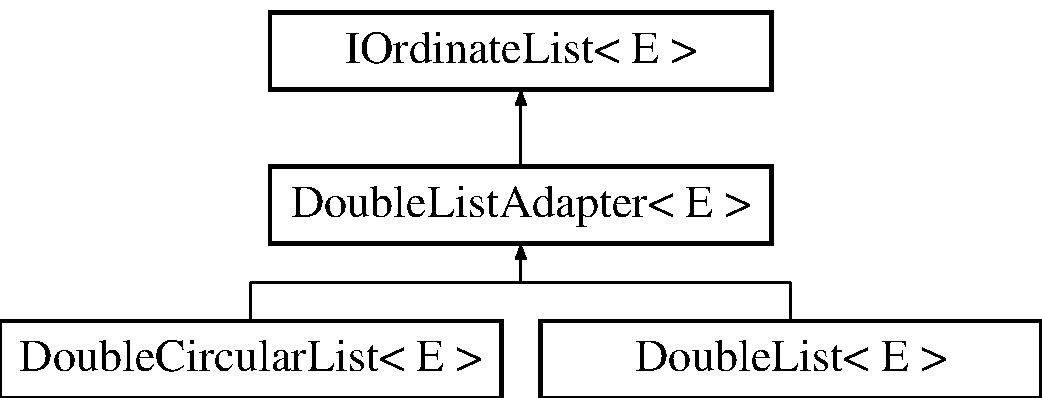
\includegraphics[height=3.000000cm]{class_double_list_adapter}
\end{center}
\end{figure}
\subsection*{Public Member Functions}
\begin{DoxyCompactItemize}
\item 
bool \hyperlink{class_double_list_adapter_a6f5bc523f04b3b223f259a72a1975b11}{add} (E p\-Data)
\item 
bool \hyperlink{class_double_list_adapter_a76d83f0f676236b98aa5e555a43a173b}{remove} (int p\-Index)
\item 
E \hyperlink{class_double_list_adapter_a70017142377b23a0f6ec22ac4c01aa6c}{get} (int p\-Index)
\item 
E \& \hyperlink{class_double_list_adapter_ad608ef5f6917c09899b55fc5b20d9b4b}{get\-Reference} (int p\-Index)
\item 
\hyperlink{class_i_iterator}{I\-Iterator}$<$ E $>$ $\ast$ \hyperlink{class_double_list_adapter_a40ba21fc70df64e91bf269bb721d20a9}{get\-Iterator} ()
\item 
void \hyperlink{class_double_list_adapter_a95df61b73f8c9535c8abe227c2207ea9}{set\-Inversed\-Iteration} (bool p\-Iteration)
\item 
virtual \hyperlink{class_double_list_adapter_aeff19b80530a522fadcea251abc63ea6}{$\sim$\-Double\-List\-Adapter} ()
\item 
void \hyperlink{class_double_list_adapter_a7f67c49e4d93576b9ccbf3578904df30}{print} ()
\end{DoxyCompactItemize}
\subsection*{Protected Member Functions}
\begin{DoxyCompactItemize}
\item 
virtual bool \hyperlink{class_double_list_adapter_a74a41e06683241f5a7d9b9d0ed38eaf9}{addi} (E p\-Data)=0
\item 
virtual bool \hyperlink{class_double_list_adapter_adf4e6a8a4479d1fa0e692aea0d254c0f}{addf} (E p\-Data)=0
\item 
virtual bool \hyperlink{class_double_list_adapter_a024ff60d5cb3e11ff5be795f48deaac0}{add\-First\-Data} (E p\-Data)=0
\item 
virtual bool \hyperlink{class_double_list_adapter_a710e75ff353e5e94ae1fb9eadc0b582b}{removei} ()=0
\item 
virtual bool \hyperlink{class_double_list_adapter_a1f069987bb3e8abcccf24659474960c3}{removef} ()=0
\end{DoxyCompactItemize}
\subsection*{Protected Attributes}
\begin{DoxyCompactItemize}
\item 
\hyperlink{class_double_node}{Double\-Node}$<$ E $>$ $\ast$ \hyperlink{class_double_list_adapter_a1c01340613e7545d5ab74286686053fa}{\-\_\-head}
\item 
\hyperlink{class_double_node}{Double\-Node}$<$ E $>$ $\ast$ \hyperlink{class_double_list_adapter_a68c6a578e4668b8c28895ac271c4c2b9}{\-\_\-tail}
\end{DoxyCompactItemize}


\subsection{Constructor \& Destructor Documentation}
\hypertarget{class_double_list_adapter_aeff19b80530a522fadcea251abc63ea6}{\index{Double\-List\-Adapter@{Double\-List\-Adapter}!$\sim$\-Double\-List\-Adapter@{$\sim$\-Double\-List\-Adapter}}
\index{$\sim$\-Double\-List\-Adapter@{$\sim$\-Double\-List\-Adapter}!DoubleListAdapter@{Double\-List\-Adapter}}
\subsubsection[{$\sim$\-Double\-List\-Adapter}]{\setlength{\rightskip}{0pt plus 5cm}template$<$class E $>$ {\bf Double\-List\-Adapter}$<$ E $>$\-::$\sim${\bf Double\-List\-Adapter} (
\begin{DoxyParamCaption}
{}
\end{DoxyParamCaption}
)\hspace{0.3cm}{\ttfamily [virtual]}}}\label{class_double_list_adapter_aeff19b80530a522fadcea251abc63ea6}


\subsection{Member Function Documentation}
\hypertarget{class_double_list_adapter_a6f5bc523f04b3b223f259a72a1975b11}{\index{Double\-List\-Adapter@{Double\-List\-Adapter}!add@{add}}
\index{add@{add}!DoubleListAdapter@{Double\-List\-Adapter}}
\subsubsection[{add}]{\setlength{\rightskip}{0pt plus 5cm}template$<$class E $>$ bool {\bf Double\-List\-Adapter}$<$ E $>$\-::add (
\begin{DoxyParamCaption}
\item[{E}]{p\-Data}
\end{DoxyParamCaption}
)\hspace{0.3cm}{\ttfamily [virtual]}}}\label{class_double_list_adapter_a6f5bc523f04b3b223f259a72a1975b11}


Implements \hyperlink{class_i_ordinate_list_af158c9cda23201b2a17e857ffcdf4cdd}{I\-Ordinate\-List$<$ E $>$}.

\hypertarget{class_double_list_adapter_adf4e6a8a4479d1fa0e692aea0d254c0f}{\index{Double\-List\-Adapter@{Double\-List\-Adapter}!addf@{addf}}
\index{addf@{addf}!DoubleListAdapter@{Double\-List\-Adapter}}
\subsubsection[{addf}]{\setlength{\rightskip}{0pt plus 5cm}template$<$class E $>$ virtual bool {\bf Double\-List\-Adapter}$<$ E $>$\-::addf (
\begin{DoxyParamCaption}
\item[{E}]{p\-Data}
\end{DoxyParamCaption}
)\hspace{0.3cm}{\ttfamily [protected]}, {\ttfamily [pure virtual]}}}\label{class_double_list_adapter_adf4e6a8a4479d1fa0e692aea0d254c0f}


Implemented in \hyperlink{class_double_circular_list_a4a6ec7a7298470389b88b0c775a9bace}{Double\-Circular\-List$<$ E $>$}, and \hyperlink{class_double_list_a495cbf66dc7f7523e15405b762cc616d}{Double\-List$<$ E $>$}.

\hypertarget{class_double_list_adapter_a024ff60d5cb3e11ff5be795f48deaac0}{\index{Double\-List\-Adapter@{Double\-List\-Adapter}!add\-First\-Data@{add\-First\-Data}}
\index{add\-First\-Data@{add\-First\-Data}!DoubleListAdapter@{Double\-List\-Adapter}}
\subsubsection[{add\-First\-Data}]{\setlength{\rightskip}{0pt plus 5cm}template$<$class E $>$ virtual bool {\bf Double\-List\-Adapter}$<$ E $>$\-::add\-First\-Data (
\begin{DoxyParamCaption}
\item[{E}]{p\-Data}
\end{DoxyParamCaption}
)\hspace{0.3cm}{\ttfamily [protected]}, {\ttfamily [pure virtual]}}}\label{class_double_list_adapter_a024ff60d5cb3e11ff5be795f48deaac0}


Implemented in \hyperlink{class_double_circular_list_aff5a0088509cc88dccfe31389d48f19e}{Double\-Circular\-List$<$ E $>$}, and \hyperlink{class_double_list_a4d72bc061da9183185b9ae1896b2767b}{Double\-List$<$ E $>$}.

\hypertarget{class_double_list_adapter_a74a41e06683241f5a7d9b9d0ed38eaf9}{\index{Double\-List\-Adapter@{Double\-List\-Adapter}!addi@{addi}}
\index{addi@{addi}!DoubleListAdapter@{Double\-List\-Adapter}}
\subsubsection[{addi}]{\setlength{\rightskip}{0pt plus 5cm}template$<$class E $>$ virtual bool {\bf Double\-List\-Adapter}$<$ E $>$\-::addi (
\begin{DoxyParamCaption}
\item[{E}]{p\-Data}
\end{DoxyParamCaption}
)\hspace{0.3cm}{\ttfamily [protected]}, {\ttfamily [pure virtual]}}}\label{class_double_list_adapter_a74a41e06683241f5a7d9b9d0ed38eaf9}


Implemented in \hyperlink{class_double_circular_list_ade2ef68a86a8deef4cb43d38e031906b}{Double\-Circular\-List$<$ E $>$}, \hyperlink{class_double_list_a621684e61b8d9d41cd107174d9877b1e}{Double\-List$<$ E $>$}, \hyperlink{class_double_circular_list_aee387acc4f53773302be4aa98bc779dc}{Double\-Circular\-List$<$ E $>$}, and \hyperlink{class_double_list_a01623cc4b04d94c655de62ae373963b2}{Double\-List$<$ E $>$}.

\hypertarget{class_double_list_adapter_a70017142377b23a0f6ec22ac4c01aa6c}{\index{Double\-List\-Adapter@{Double\-List\-Adapter}!get@{get}}
\index{get@{get}!DoubleListAdapter@{Double\-List\-Adapter}}
\subsubsection[{get}]{\setlength{\rightskip}{0pt plus 5cm}template$<$class E $>$ E {\bf Double\-List\-Adapter}$<$ E $>$\-::get (
\begin{DoxyParamCaption}
\item[{int}]{p\-Index}
\end{DoxyParamCaption}
)\hspace{0.3cm}{\ttfamily [virtual]}}}\label{class_double_list_adapter_a70017142377b23a0f6ec22ac4c01aa6c}


Implements \hyperlink{class_i_ordinate_list_aef65b00ca705d1b106d51bff512b2021}{I\-Ordinate\-List$<$ E $>$}.

\hypertarget{class_double_list_adapter_a40ba21fc70df64e91bf269bb721d20a9}{\index{Double\-List\-Adapter@{Double\-List\-Adapter}!get\-Iterator@{get\-Iterator}}
\index{get\-Iterator@{get\-Iterator}!DoubleListAdapter@{Double\-List\-Adapter}}
\subsubsection[{get\-Iterator}]{\setlength{\rightskip}{0pt plus 5cm}template$<$class E $>$ {\bf I\-Iterator}$<$ E $>$ $\ast$ {\bf Double\-List\-Adapter}$<$ E $>$\-::get\-Iterator (
\begin{DoxyParamCaption}
{}
\end{DoxyParamCaption}
)\hspace{0.3cm}{\ttfamily [virtual]}}}\label{class_double_list_adapter_a40ba21fc70df64e91bf269bb721d20a9}


Implements \hyperlink{class_i_ordinate_list_aa555ab647394d5bf06bb4f38715bd167}{I\-Ordinate\-List$<$ E $>$}.

\hypertarget{class_double_list_adapter_ad608ef5f6917c09899b55fc5b20d9b4b}{\index{Double\-List\-Adapter@{Double\-List\-Adapter}!get\-Reference@{get\-Reference}}
\index{get\-Reference@{get\-Reference}!DoubleListAdapter@{Double\-List\-Adapter}}
\subsubsection[{get\-Reference}]{\setlength{\rightskip}{0pt plus 5cm}template$<$class E $>$ E \& {\bf Double\-List\-Adapter}$<$ E $>$\-::get\-Reference (
\begin{DoxyParamCaption}
\item[{int}]{p\-Index}
\end{DoxyParamCaption}
)\hspace{0.3cm}{\ttfamily [virtual]}}}\label{class_double_list_adapter_ad608ef5f6917c09899b55fc5b20d9b4b}


Implements \hyperlink{class_i_ordinate_list_a126adb3087d227a7bd47288002c6d48e}{I\-Ordinate\-List$<$ E $>$}.

\hypertarget{class_double_list_adapter_a7f67c49e4d93576b9ccbf3578904df30}{\index{Double\-List\-Adapter@{Double\-List\-Adapter}!print@{print}}
\index{print@{print}!DoubleListAdapter@{Double\-List\-Adapter}}
\subsubsection[{print}]{\setlength{\rightskip}{0pt plus 5cm}template$<$class E $>$ void {\bf Double\-List\-Adapter}$<$ E $>$\-::print (
\begin{DoxyParamCaption}
{}
\end{DoxyParamCaption}
)}}\label{class_double_list_adapter_a7f67c49e4d93576b9ccbf3578904df30}
\hypertarget{class_double_list_adapter_a76d83f0f676236b98aa5e555a43a173b}{\index{Double\-List\-Adapter@{Double\-List\-Adapter}!remove@{remove}}
\index{remove@{remove}!DoubleListAdapter@{Double\-List\-Adapter}}
\subsubsection[{remove}]{\setlength{\rightskip}{0pt plus 5cm}template$<$class E $>$ bool {\bf Double\-List\-Adapter}$<$ E $>$\-::remove (
\begin{DoxyParamCaption}
\item[{int}]{p\-Index}
\end{DoxyParamCaption}
)\hspace{0.3cm}{\ttfamily [virtual]}}}\label{class_double_list_adapter_a76d83f0f676236b98aa5e555a43a173b}


Implements \hyperlink{class_i_ordinate_list_a1015be27579a09c4805505ea3e4c4752}{I\-Ordinate\-List$<$ E $>$}.

\hypertarget{class_double_list_adapter_a1f069987bb3e8abcccf24659474960c3}{\index{Double\-List\-Adapter@{Double\-List\-Adapter}!removef@{removef}}
\index{removef@{removef}!DoubleListAdapter@{Double\-List\-Adapter}}
\subsubsection[{removef}]{\setlength{\rightskip}{0pt plus 5cm}template$<$class E $>$ virtual bool {\bf Double\-List\-Adapter}$<$ E $>$\-::removef (
\begin{DoxyParamCaption}
{}
\end{DoxyParamCaption}
)\hspace{0.3cm}{\ttfamily [protected]}, {\ttfamily [pure virtual]}}}\label{class_double_list_adapter_a1f069987bb3e8abcccf24659474960c3}


Implemented in \hyperlink{class_double_circular_list_a937da114318f91c6013dd4543636da9d}{Double\-Circular\-List$<$ E $>$}, and \hyperlink{class_double_list_a0cd7c06fa533e3f800778920346b8a7b}{Double\-List$<$ E $>$}.

\hypertarget{class_double_list_adapter_a710e75ff353e5e94ae1fb9eadc0b582b}{\index{Double\-List\-Adapter@{Double\-List\-Adapter}!removei@{removei}}
\index{removei@{removei}!DoubleListAdapter@{Double\-List\-Adapter}}
\subsubsection[{removei}]{\setlength{\rightskip}{0pt plus 5cm}template$<$class E $>$ virtual bool {\bf Double\-List\-Adapter}$<$ E $>$\-::removei (
\begin{DoxyParamCaption}
{}
\end{DoxyParamCaption}
)\hspace{0.3cm}{\ttfamily [protected]}, {\ttfamily [pure virtual]}}}\label{class_double_list_adapter_a710e75ff353e5e94ae1fb9eadc0b582b}


Implemented in \hyperlink{class_double_circular_list_a1d2c6f1fec95c8d2887c54cb3fc3ff84}{Double\-Circular\-List$<$ E $>$}, and \hyperlink{class_double_list_a074473aaac863a9e00ec34c2316a2d9e}{Double\-List$<$ E $>$}.

\hypertarget{class_double_list_adapter_a95df61b73f8c9535c8abe227c2207ea9}{\index{Double\-List\-Adapter@{Double\-List\-Adapter}!set\-Inversed\-Iteration@{set\-Inversed\-Iteration}}
\index{set\-Inversed\-Iteration@{set\-Inversed\-Iteration}!DoubleListAdapter@{Double\-List\-Adapter}}
\subsubsection[{set\-Inversed\-Iteration}]{\setlength{\rightskip}{0pt plus 5cm}template$<$class E $>$ void {\bf Double\-List\-Adapter}$<$ E $>$\-::set\-Inversed\-Iteration (
\begin{DoxyParamCaption}
\item[{bool}]{p\-Iteration}
\end{DoxyParamCaption}
)}}\label{class_double_list_adapter_a95df61b73f8c9535c8abe227c2207ea9}


\subsection{Member Data Documentation}
\hypertarget{class_double_list_adapter_a1c01340613e7545d5ab74286686053fa}{\index{Double\-List\-Adapter@{Double\-List\-Adapter}!\-\_\-head@{\-\_\-head}}
\index{\-\_\-head@{\-\_\-head}!DoubleListAdapter@{Double\-List\-Adapter}}
\subsubsection[{\-\_\-head}]{\setlength{\rightskip}{0pt plus 5cm}template$<$class E $>$ {\bf Double\-Node}$<$E$>$$\ast$ {\bf Double\-List\-Adapter}$<$ E $>$\-::\-\_\-head\hspace{0.3cm}{\ttfamily [protected]}}}\label{class_double_list_adapter_a1c01340613e7545d5ab74286686053fa}
\hypertarget{class_double_list_adapter_a68c6a578e4668b8c28895ac271c4c2b9}{\index{Double\-List\-Adapter@{Double\-List\-Adapter}!\-\_\-tail@{\-\_\-tail}}
\index{\-\_\-tail@{\-\_\-tail}!DoubleListAdapter@{Double\-List\-Adapter}}
\subsubsection[{\-\_\-tail}]{\setlength{\rightskip}{0pt plus 5cm}template$<$class E $>$ {\bf Double\-Node}$<$E$>$ $\ast$ {\bf Double\-List\-Adapter}$<$ E $>$\-::\-\_\-tail\hspace{0.3cm}{\ttfamily [protected]}}}\label{class_double_list_adapter_a68c6a578e4668b8c28895ac271c4c2b9}


The documentation for this class was generated from the following file\-:\begin{DoxyCompactItemize}
\item 
ordinate\-List/\hyperlink{doublelistadapter_8h}{doublelistadapter.\-h}\end{DoxyCompactItemize}

\hypertarget{class_double_node}{\section{Double\-Node$<$ E $>$ Class Template Reference}
\label{class_double_node}\index{Double\-Node$<$ E $>$@{Double\-Node$<$ E $>$}}
}


Es la parte elemental de una lista que sea doublemente enlazada.  




{\ttfamily \#include $<$Double\-Node.\-h$>$}

\subsection*{Public Member Functions}
\begin{DoxyCompactItemize}
\item 
\hyperlink{class_double_node_a915ac8a626f09ec53db64b7c5b294b2d}{Double\-Node} (E)
\begin{DoxyCompactList}\small\item\em Constructor del Nodo Doble, el dato previous y next se setean como punteros nulos para evitar punteros colgados. \end{DoxyCompactList}\item 
\hyperlink{class_double_node_a53d29dbf397d39b420f64ab943b62cee}{Double\-Node} (E, \hyperlink{class_double_node}{Double\-Node}$<$ E $>$ $\ast$, \hyperlink{class_double_node}{Double\-Node}$<$ E $>$ $\ast$)
\begin{DoxyCompactList}\small\item\em Constructor del Nodo Doble. \end{DoxyCompactList}\item 
void \hyperlink{class_double_node_a21f86a81b7d4e4db966e07ce06da4f3a}{set\-Data} (E)
\begin{DoxyCompactList}\small\item\em Setea el dato contenido en el nodo. \end{DoxyCompactList}\item 
E \hyperlink{class_double_node_a59310f31d21f431febc4d329e1f10699}{get\-Data} () const 
\begin{DoxyCompactList}\small\item\em Obtiene el dato contenido en el nodo. \end{DoxyCompactList}\item 
\hypertarget{class_double_node_ac6b096a9a3a404f73e26b7319372fcbb}{E \& {\bfseries get\-Reference\-Data} ()}\label{class_double_node_ac6b096a9a3a404f73e26b7319372fcbb}

\item 
void \hyperlink{class_double_node_aba52422e27040e524ba629445e9d8b93}{set\-Next} (\hyperlink{class_double_node}{Double\-Node}$<$ E $>$ $\ast$)
\begin{DoxyCompactList}\small\item\em Setea el puntero del nodo siguiente. \end{DoxyCompactList}\item 
\hyperlink{class_double_node}{Double\-Node}$<$ E $>$ $\ast$ \hyperlink{class_double_node_af5af4a30419b7a7c746361c1476e119f}{get\-Next} () const 
\begin{DoxyCompactList}\small\item\em Obtiene el nodo siguiente. \end{DoxyCompactList}\item 
void \hyperlink{class_double_node_aa76c202fdfd533984d9e9ae1892d194d}{set\-Previous} (\hyperlink{class_double_node}{Double\-Node}$<$ E $>$ $\ast$)
\begin{DoxyCompactList}\small\item\em Setea el puntero del nodo anterior. \end{DoxyCompactList}\item 
\hyperlink{class_double_node}{Double\-Node}$<$ E $>$ $\ast$ \hyperlink{class_double_node_a86c75b7ed7e944f9748363fe23b2518e}{get\-Previous} () const 
\begin{DoxyCompactList}\small\item\em Obtiene el nodo anterior. \end{DoxyCompactList}\item 
\hypertarget{class_double_node_abd78f421a570cd0fb0cecfedb979d799}{virtual \hyperlink{class_double_node_abd78f421a570cd0fb0cecfedb979d799}{$\sim$\-Double\-Node} ()}\label{class_double_node_abd78f421a570cd0fb0cecfedb979d799}

\begin{DoxyCompactList}\small\item\em el destructor de este nodo \end{DoxyCompactList}\end{DoxyCompactItemize}


\subsection{Detailed Description}
\subsubsection*{template$<$class E$>$class Double\-Node$<$ E $>$}

Es la parte elemental de una lista que sea doublemente enlazada. 

\subsection{Constructor \& Destructor Documentation}
\hypertarget{class_double_node_a915ac8a626f09ec53db64b7c5b294b2d}{\index{Double\-Node@{Double\-Node}!Double\-Node@{Double\-Node}}
\index{Double\-Node@{Double\-Node}!DoubleNode@{Double\-Node}}
\subsubsection[{Double\-Node}]{\setlength{\rightskip}{0pt plus 5cm}template$<$class E $>$ {\bf Double\-Node}$<$ E $>$\-::{\bf Double\-Node} (
\begin{DoxyParamCaption}
\item[{E}]{data}
\end{DoxyParamCaption}
)}}\label{class_double_node_a915ac8a626f09ec53db64b7c5b294b2d}


Constructor del Nodo Doble, el dato previous y next se setean como punteros nulos para evitar punteros colgados. 


\begin{DoxyParams}{Parameters}
{\em data} & el dato que contrendra el nodo \\
\hline
\end{DoxyParams}
\hypertarget{class_double_node_a53d29dbf397d39b420f64ab943b62cee}{\index{Double\-Node@{Double\-Node}!Double\-Node@{Double\-Node}}
\index{Double\-Node@{Double\-Node}!DoubleNode@{Double\-Node}}
\subsubsection[{Double\-Node}]{\setlength{\rightskip}{0pt plus 5cm}template$<$class E $>$ {\bf Double\-Node}$<$ E $>$\-::{\bf Double\-Node} (
\begin{DoxyParamCaption}
\item[{E}]{data, }
\item[{{\bf Double\-Node}$<$ E $>$ $\ast$}]{previous, }
\item[{{\bf Double\-Node}$<$ E $>$ $\ast$}]{next}
\end{DoxyParamCaption}
)}}\label{class_double_node_a53d29dbf397d39b420f64ab943b62cee}


Constructor del Nodo Doble. 


\begin{DoxyParams}{Parameters}
{\em data} & el dato que contendra el dato \\
\hline
{\em previous} & el puntero al nodo anterior \\
\hline
{\em next} & el puntero al nodo siguiente \\
\hline
\end{DoxyParams}


\subsection{Member Function Documentation}
\hypertarget{class_double_node_a59310f31d21f431febc4d329e1f10699}{\index{Double\-Node@{Double\-Node}!get\-Data@{get\-Data}}
\index{get\-Data@{get\-Data}!DoubleNode@{Double\-Node}}
\subsubsection[{get\-Data}]{\setlength{\rightskip}{0pt plus 5cm}template$<$class E $>$ E {\bf Double\-Node}$<$ E $>$\-::get\-Data (
\begin{DoxyParamCaption}
{}
\end{DoxyParamCaption}
) const}}\label{class_double_node_a59310f31d21f431febc4d329e1f10699}


Obtiene el dato contenido en el nodo. 

\begin{DoxyReturn}{Returns}
E el dato contenido 
\end{DoxyReturn}
\hypertarget{class_double_node_af5af4a30419b7a7c746361c1476e119f}{\index{Double\-Node@{Double\-Node}!get\-Next@{get\-Next}}
\index{get\-Next@{get\-Next}!DoubleNode@{Double\-Node}}
\subsubsection[{get\-Next}]{\setlength{\rightskip}{0pt plus 5cm}template$<$class E $>$ {\bf Double\-Node}$<$ E $>$ $\ast$ {\bf Double\-Node}$<$ E $>$\-::get\-Next (
\begin{DoxyParamCaption}
{}
\end{DoxyParamCaption}
) const}}\label{class_double_node_af5af4a30419b7a7c746361c1476e119f}


Obtiene el nodo siguiente. 

\begin{DoxyReturn}{Returns}
Double\-Node$<$\-E$>$ el nodo siguiente 
\end{DoxyReturn}
\hypertarget{class_double_node_a86c75b7ed7e944f9748363fe23b2518e}{\index{Double\-Node@{Double\-Node}!get\-Previous@{get\-Previous}}
\index{get\-Previous@{get\-Previous}!DoubleNode@{Double\-Node}}
\subsubsection[{get\-Previous}]{\setlength{\rightskip}{0pt plus 5cm}template$<$class E $>$ {\bf Double\-Node}$<$ E $>$ $\ast$ {\bf Double\-Node}$<$ E $>$\-::get\-Previous (
\begin{DoxyParamCaption}
{}
\end{DoxyParamCaption}
) const}}\label{class_double_node_a86c75b7ed7e944f9748363fe23b2518e}


Obtiene el nodo anterior. 

\begin{DoxyReturn}{Returns}
Double\-Node$<$\-E$>$ el nodo anterior 
\end{DoxyReturn}
\hypertarget{class_double_node_a21f86a81b7d4e4db966e07ce06da4f3a}{\index{Double\-Node@{Double\-Node}!set\-Data@{set\-Data}}
\index{set\-Data@{set\-Data}!DoubleNode@{Double\-Node}}
\subsubsection[{set\-Data}]{\setlength{\rightskip}{0pt plus 5cm}template$<$class E $>$ void {\bf Double\-Node}$<$ E $>$\-::set\-Data (
\begin{DoxyParamCaption}
\item[{E}]{data}
\end{DoxyParamCaption}
)}}\label{class_double_node_a21f86a81b7d4e4db966e07ce06da4f3a}


Setea el dato contenido en el nodo. 


\begin{DoxyParams}{Parameters}
{\em data} & el dato nuevo \\
\hline
\end{DoxyParams}
\hypertarget{class_double_node_aba52422e27040e524ba629445e9d8b93}{\index{Double\-Node@{Double\-Node}!set\-Next@{set\-Next}}
\index{set\-Next@{set\-Next}!DoubleNode@{Double\-Node}}
\subsubsection[{set\-Next}]{\setlength{\rightskip}{0pt plus 5cm}template$<$class E $>$ void {\bf Double\-Node}$<$ E $>$\-::set\-Next (
\begin{DoxyParamCaption}
\item[{{\bf Double\-Node}$<$ E $>$ $\ast$}]{next}
\end{DoxyParamCaption}
)}}\label{class_double_node_aba52422e27040e524ba629445e9d8b93}


Setea el puntero del nodo siguiente. 


\begin{DoxyParams}{Parameters}
{\em next} & el nuevo nodo que representa el nodo siguiente \\
\hline
\end{DoxyParams}
\hypertarget{class_double_node_aa76c202fdfd533984d9e9ae1892d194d}{\index{Double\-Node@{Double\-Node}!set\-Previous@{set\-Previous}}
\index{set\-Previous@{set\-Previous}!DoubleNode@{Double\-Node}}
\subsubsection[{set\-Previous}]{\setlength{\rightskip}{0pt plus 5cm}template$<$class E $>$ void {\bf Double\-Node}$<$ E $>$\-::set\-Previous (
\begin{DoxyParamCaption}
\item[{{\bf Double\-Node}$<$ E $>$ $\ast$}]{previous}
\end{DoxyParamCaption}
)}}\label{class_double_node_aa76c202fdfd533984d9e9ae1892d194d}


Setea el puntero del nodo anterior. 


\begin{DoxyParams}{Parameters}
{\em previous} & el nuevo nodo que reprenta el nodo anterior \\
\hline
\end{DoxyParams}


The documentation for this class was generated from the following file\-:\begin{DoxyCompactItemize}
\item 
list/Double\-Node.\-h\end{DoxyCompactItemize}

\hypertarget{class_enemy_rocket}{\section{Enemy\-Rocket Class Reference}
\label{class_enemy_rocket}\index{Enemy\-Rocket@{Enemy\-Rocket}}
}


{\ttfamily \#include $<$enemyrocket.\-h$>$}

Inheritance diagram for Enemy\-Rocket\-:\begin{figure}[H]
\begin{center}
\leavevmode
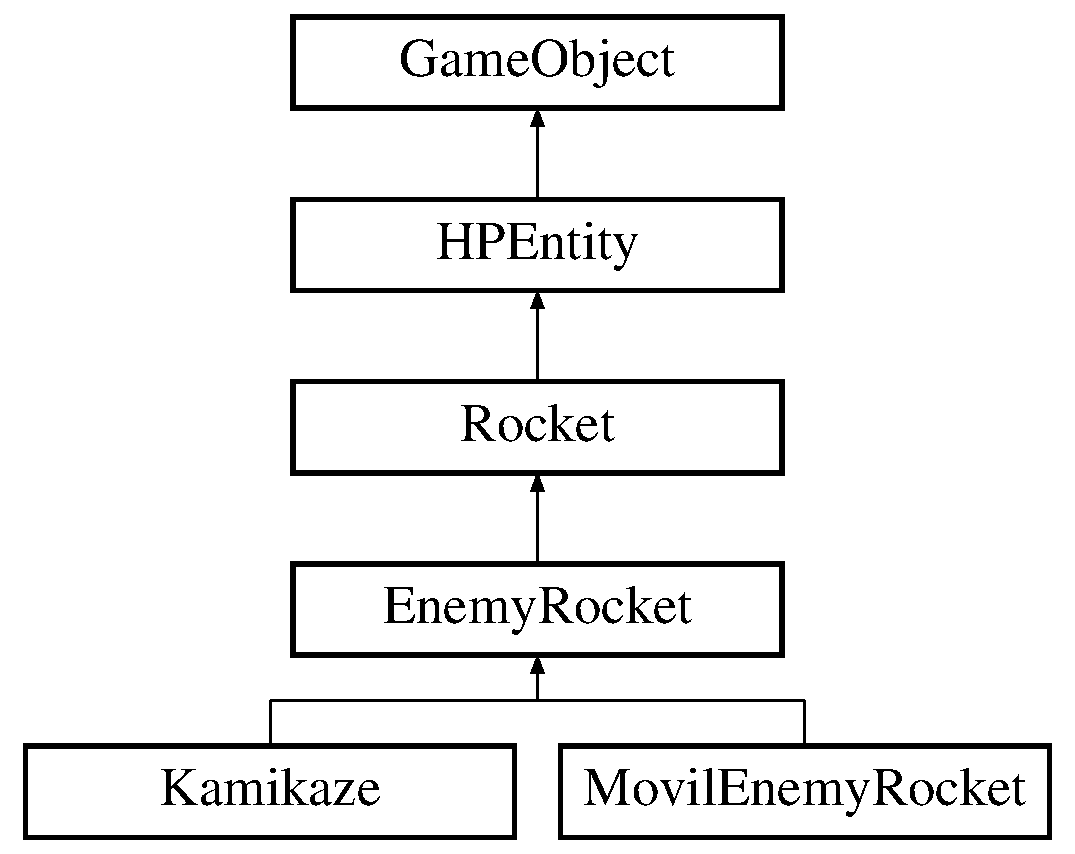
\includegraphics[height=5.000000cm]{class_enemy_rocket}
\end{center}
\end{figure}
\subsection*{Public Member Functions}
\begin{DoxyCompactItemize}
\item 
\hyperlink{class_enemy_rocket_a602b0809840648ca73f620968499df55}{Enemy\-Rocket} (Q\-Rect p\-Rectangle, int p\-Max\-Hp)
\item 
\hyperlink{class_shot}{Shot} $\ast$ \hyperlink{class_enemy_rocket_aaa119ae66d24f37445ee53f0e2184bc2}{shoot} ()
\item 
virtual int \hyperlink{class_enemy_rocket_a44e857f29c0846545743e21638391527}{get\-Enemy\-Type} ()=0
\item 
virtual \hyperlink{class_enemy_rocket_abb973e1ee2e99a06789131b1dd3180ab}{$\sim$\-Enemy\-Rocket} ()
\end{DoxyCompactItemize}
\subsection*{Static Public Attributes}
\begin{DoxyCompactItemize}
\item 
static const int \hyperlink{class_enemy_rocket_a15caca840f5e774985fecf4295d9446d}{K\-A\-M\-I\-K\-A\-Z\-E} = 1
\item 
static const int \hyperlink{class_enemy_rocket_a62103a6d3bc8dd2860b91d5250113281}{M\-O\-V\-I\-L\-\_\-\-E\-N\-E\-M\-Y\-\_\-\-R\-O\-C\-K\-E\-T} = 0
\end{DoxyCompactItemize}
\subsection*{Additional Inherited Members}


\subsection{Constructor \& Destructor Documentation}
\hypertarget{class_enemy_rocket_a602b0809840648ca73f620968499df55}{\index{Enemy\-Rocket@{Enemy\-Rocket}!Enemy\-Rocket@{Enemy\-Rocket}}
\index{Enemy\-Rocket@{Enemy\-Rocket}!EnemyRocket@{Enemy\-Rocket}}
\subsubsection[{Enemy\-Rocket}]{\setlength{\rightskip}{0pt plus 5cm}Enemy\-Rocket\-::\-Enemy\-Rocket (
\begin{DoxyParamCaption}
\item[{Q\-Rect}]{p\-Rectangle, }
\item[{int}]{p\-Max\-Hp}
\end{DoxyParamCaption}
)}}\label{class_enemy_rocket_a602b0809840648ca73f620968499df55}
\hypertarget{class_enemy_rocket_abb973e1ee2e99a06789131b1dd3180ab}{\index{Enemy\-Rocket@{Enemy\-Rocket}!$\sim$\-Enemy\-Rocket@{$\sim$\-Enemy\-Rocket}}
\index{$\sim$\-Enemy\-Rocket@{$\sim$\-Enemy\-Rocket}!EnemyRocket@{Enemy\-Rocket}}
\subsubsection[{$\sim$\-Enemy\-Rocket}]{\setlength{\rightskip}{0pt plus 5cm}Enemy\-Rocket\-::$\sim$\-Enemy\-Rocket (
\begin{DoxyParamCaption}
{}
\end{DoxyParamCaption}
)\hspace{0.3cm}{\ttfamily [virtual]}}}\label{class_enemy_rocket_abb973e1ee2e99a06789131b1dd3180ab}


\subsection{Member Function Documentation}
\hypertarget{class_enemy_rocket_a44e857f29c0846545743e21638391527}{\index{Enemy\-Rocket@{Enemy\-Rocket}!get\-Enemy\-Type@{get\-Enemy\-Type}}
\index{get\-Enemy\-Type@{get\-Enemy\-Type}!EnemyRocket@{Enemy\-Rocket}}
\subsubsection[{get\-Enemy\-Type}]{\setlength{\rightskip}{0pt plus 5cm}virtual int Enemy\-Rocket\-::get\-Enemy\-Type (
\begin{DoxyParamCaption}
{}
\end{DoxyParamCaption}
)\hspace{0.3cm}{\ttfamily [pure virtual]}}}\label{class_enemy_rocket_a44e857f29c0846545743e21638391527}


Implemented in \hyperlink{class_kamikaze_ae82e6a48d3e927c65fcd64269a533377}{Kamikaze}, and \hyperlink{class_movil_enemy_rocket_a6372ff2e56ce1494f3e3e2420706ef3e}{Movil\-Enemy\-Rocket}.

\hypertarget{class_enemy_rocket_aaa119ae66d24f37445ee53f0e2184bc2}{\index{Enemy\-Rocket@{Enemy\-Rocket}!shoot@{shoot}}
\index{shoot@{shoot}!EnemyRocket@{Enemy\-Rocket}}
\subsubsection[{shoot}]{\setlength{\rightskip}{0pt plus 5cm}{\bf Shot} $\ast$ Enemy\-Rocket\-::shoot (
\begin{DoxyParamCaption}
{}
\end{DoxyParamCaption}
)\hspace{0.3cm}{\ttfamily [virtual]}}}\label{class_enemy_rocket_aaa119ae66d24f37445ee53f0e2184bc2}


Implements \hyperlink{class_rocket_a5164f5926f96291b57da2516d46262e8}{Rocket}.



\subsection{Member Data Documentation}
\hypertarget{class_enemy_rocket_a15caca840f5e774985fecf4295d9446d}{\index{Enemy\-Rocket@{Enemy\-Rocket}!K\-A\-M\-I\-K\-A\-Z\-E@{K\-A\-M\-I\-K\-A\-Z\-E}}
\index{K\-A\-M\-I\-K\-A\-Z\-E@{K\-A\-M\-I\-K\-A\-Z\-E}!EnemyRocket@{Enemy\-Rocket}}
\subsubsection[{K\-A\-M\-I\-K\-A\-Z\-E}]{\setlength{\rightskip}{0pt plus 5cm}const int Enemy\-Rocket\-::\-K\-A\-M\-I\-K\-A\-Z\-E = 1\hspace{0.3cm}{\ttfamily [static]}}}\label{class_enemy_rocket_a15caca840f5e774985fecf4295d9446d}
\hypertarget{class_enemy_rocket_a62103a6d3bc8dd2860b91d5250113281}{\index{Enemy\-Rocket@{Enemy\-Rocket}!M\-O\-V\-I\-L\-\_\-\-E\-N\-E\-M\-Y\-\_\-\-R\-O\-C\-K\-E\-T@{M\-O\-V\-I\-L\-\_\-\-E\-N\-E\-M\-Y\-\_\-\-R\-O\-C\-K\-E\-T}}
\index{M\-O\-V\-I\-L\-\_\-\-E\-N\-E\-M\-Y\-\_\-\-R\-O\-C\-K\-E\-T@{M\-O\-V\-I\-L\-\_\-\-E\-N\-E\-M\-Y\-\_\-\-R\-O\-C\-K\-E\-T}!EnemyRocket@{Enemy\-Rocket}}
\subsubsection[{M\-O\-V\-I\-L\-\_\-\-E\-N\-E\-M\-Y\-\_\-\-R\-O\-C\-K\-E\-T}]{\setlength{\rightskip}{0pt plus 5cm}const int Enemy\-Rocket\-::\-M\-O\-V\-I\-L\-\_\-\-E\-N\-E\-M\-Y\-\_\-\-R\-O\-C\-K\-E\-T = 0\hspace{0.3cm}{\ttfamily [static]}}}\label{class_enemy_rocket_a62103a6d3bc8dd2860b91d5250113281}


The documentation for this class was generated from the following files\-:\begin{DoxyCompactItemize}
\item 
logic/rocket/\hyperlink{enemyrocket_8h}{enemyrocket.\-h}\item 
logic/rocket/\hyperlink{enemyrocket_8cpp}{enemyrocket.\-cpp}\end{DoxyCompactItemize}

\hypertarget{class_game_loop}{\section{Game\-Loop Class Reference}
\label{class_game_loop}\index{Game\-Loop@{Game\-Loop}}
}


Es la clase que se encarga de controlar el pintado de la ventana del juego seccionandolo en frame por segundo, especificamente 24 fps, la clase regula el pintado y la ejecucion de las actualizaciones del juego mismo.  




{\ttfamily \#include $<$gameloop.\-h$>$}

Inheritance diagram for Game\-Loop\-:\begin{figure}[H]
\begin{center}
\leavevmode
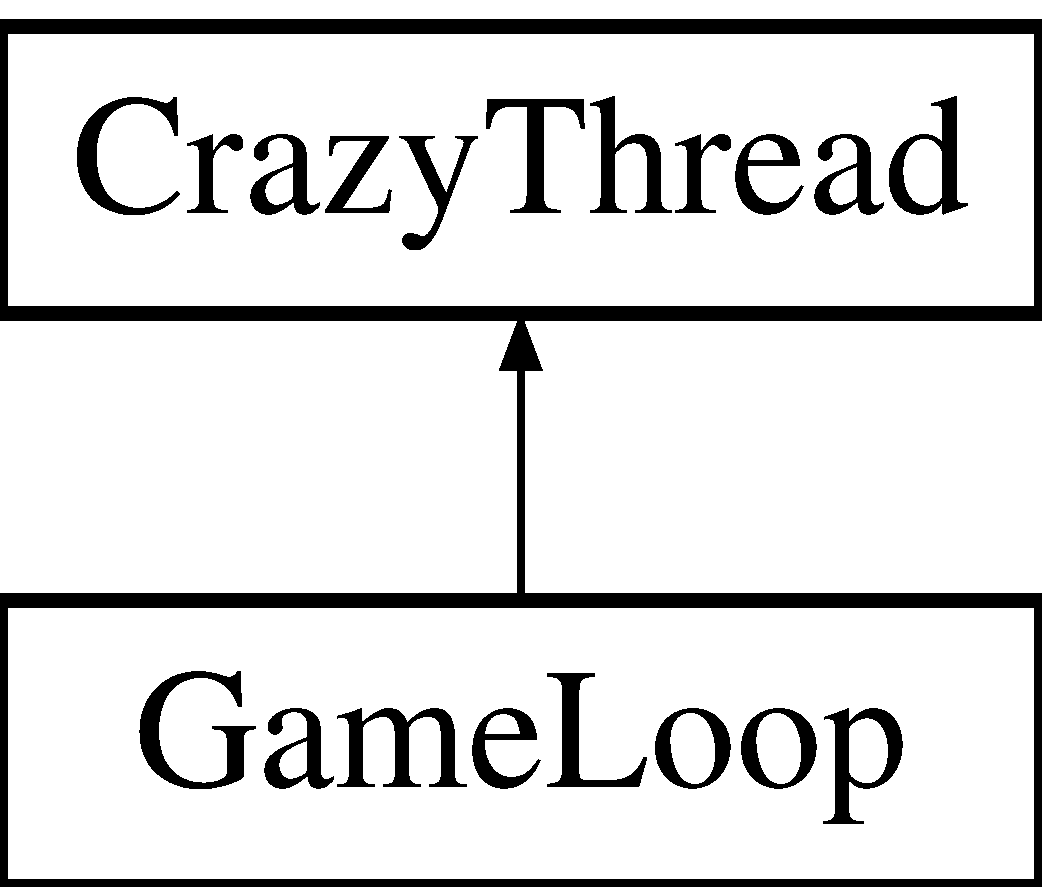
\includegraphics[height=2.000000cm]{class_game_loop}
\end{center}
\end{figure}
\subsection*{Public Member Functions}
\begin{DoxyCompactItemize}
\item 
\hyperlink{class_game_loop_adbe6559d3c3270054090db3b98a5c2d5}{Game\-Loop} (\hyperlink{class_kernel_game}{Kernel\-Game} $\ast$p\-Kernel\-Game)
\begin{DoxyCompactList}\small\item\em Es el constructor de la clase. \end{DoxyCompactList}\item 
virtual \hyperlink{class_game_loop_ae6c558d0d751a068dbafe2cae465ec1f}{$\sim$\-Game\-Loop} ()
\begin{DoxyCompactList}\small\item\em Metodo virtual destructor, se encarga de detener el thread si este no ha sido detenido para evitar problemas en tiempo de ejecucion. \end{DoxyCompactList}\item 
\hyperlink{class_thread_helper}{Thread\-Helper} $\ast$ \hyperlink{class_game_loop_aa95091d6b9fbc580219ee08374ca1642}{get\-Gui\-Conector} () const 
\begin{DoxyCompactList}\small\item\em retorna un puntero a la objeto que se encarga de conectarse con la logica \end{DoxyCompactList}\end{DoxyCompactItemize}
\subsection*{Protected Member Functions}
\begin{DoxyCompactItemize}
\item 
void \hyperlink{class_game_loop_a87ba7bf63cff924dbaec68aa41508cc0}{internal\-Run} ()
\begin{DoxyCompactList}\small\item\em Es el metodo a sobrescribir de su clase padre \hyperlink{class_crazy_thread}{Crazy\-Thread}\} El metodo se encarga de regular las actualizaciones logicas dentro del juego ademas de enviar signal para que la ventana pueda pintar estas actualizacion. \end{DoxyCompactList}\end{DoxyCompactItemize}


\subsection{Detailed Description}
Es la clase que se encarga de controlar el pintado de la ventana del juego seccionandolo en frame por segundo, especificamente 24 fps, la clase regula el pintado y la ejecucion de las actualizaciones del juego mismo. 

\subsection{Constructor \& Destructor Documentation}
\hypertarget{class_game_loop_adbe6559d3c3270054090db3b98a5c2d5}{\index{Game\-Loop@{Game\-Loop}!Game\-Loop@{Game\-Loop}}
\index{Game\-Loop@{Game\-Loop}!GameLoop@{Game\-Loop}}
\subsubsection[{Game\-Loop}]{\setlength{\rightskip}{0pt plus 5cm}Game\-Loop\-::\-Game\-Loop (
\begin{DoxyParamCaption}
\item[{{\bf Kernel\-Game} $\ast$}]{p\-Kernel\-Game}
\end{DoxyParamCaption}
)}}\label{class_game_loop_adbe6559d3c3270054090db3b98a5c2d5}


Es el constructor de la clase. 


\begin{DoxyParams}{Parameters}
{\em p\-Kernel\-Game} & es la variable que contiene la logica y la cual sera el punto centra de este thread \\
\hline
\end{DoxyParams}
\hypertarget{class_game_loop_ae6c558d0d751a068dbafe2cae465ec1f}{\index{Game\-Loop@{Game\-Loop}!$\sim$\-Game\-Loop@{$\sim$\-Game\-Loop}}
\index{$\sim$\-Game\-Loop@{$\sim$\-Game\-Loop}!GameLoop@{Game\-Loop}}
\subsubsection[{$\sim$\-Game\-Loop}]{\setlength{\rightskip}{0pt plus 5cm}Game\-Loop\-::$\sim$\-Game\-Loop (
\begin{DoxyParamCaption}
{}
\end{DoxyParamCaption}
)\hspace{0.3cm}{\ttfamily [virtual]}}}\label{class_game_loop_ae6c558d0d751a068dbafe2cae465ec1f}


Metodo virtual destructor, se encarga de detener el thread si este no ha sido detenido para evitar problemas en tiempo de ejecucion. 



\subsection{Member Function Documentation}
\hypertarget{class_game_loop_aa95091d6b9fbc580219ee08374ca1642}{\index{Game\-Loop@{Game\-Loop}!get\-Gui\-Conector@{get\-Gui\-Conector}}
\index{get\-Gui\-Conector@{get\-Gui\-Conector}!GameLoop@{Game\-Loop}}
\subsubsection[{get\-Gui\-Conector}]{\setlength{\rightskip}{0pt plus 5cm}{\bf Thread\-Helper} $\ast$ Game\-Loop\-::get\-Gui\-Conector (
\begin{DoxyParamCaption}
{}
\end{DoxyParamCaption}
) const}}\label{class_game_loop_aa95091d6b9fbc580219ee08374ca1642}


retorna un puntero a la objeto que se encarga de conectarse con la logica 

\begin{DoxyReturn}{Returns}
\hyperlink{class_thread_helper}{Thread\-Helper} el puntero que se encarga de conectarse con la logica 
\end{DoxyReturn}
\hypertarget{class_game_loop_a87ba7bf63cff924dbaec68aa41508cc0}{\index{Game\-Loop@{Game\-Loop}!internal\-Run@{internal\-Run}}
\index{internal\-Run@{internal\-Run}!GameLoop@{Game\-Loop}}
\subsubsection[{internal\-Run}]{\setlength{\rightskip}{0pt plus 5cm}void Game\-Loop\-::internal\-Run (
\begin{DoxyParamCaption}
{}
\end{DoxyParamCaption}
)\hspace{0.3cm}{\ttfamily [protected]}, {\ttfamily [virtual]}}}\label{class_game_loop_a87ba7bf63cff924dbaec68aa41508cc0}


Es el metodo a sobrescribir de su clase padre \hyperlink{class_crazy_thread}{Crazy\-Thread}\} El metodo se encarga de regular las actualizaciones logicas dentro del juego ademas de enviar signal para que la ventana pueda pintar estas actualizacion. 



Implements \hyperlink{class_crazy_thread_ac55ecbf9e17716a6dd9acd3f22e4ad80}{Crazy\-Thread}.



The documentation for this class was generated from the following files\-:\begin{DoxyCompactItemize}
\item 
logic/crazythreads/\hyperlink{gameloop_8h}{gameloop.\-h}\item 
logic/crazythreads/\hyperlink{gameloop_8cpp}{gameloop.\-cpp}\end{DoxyCompactItemize}

\hypertarget{class_game_manager}{\section{Game\-Manager Class Reference}
\label{class_game_manager}\index{Game\-Manager@{Game\-Manager}}
}
Inheritance diagram for Game\-Manager\-:\begin{figure}[H]
\begin{center}
\leavevmode
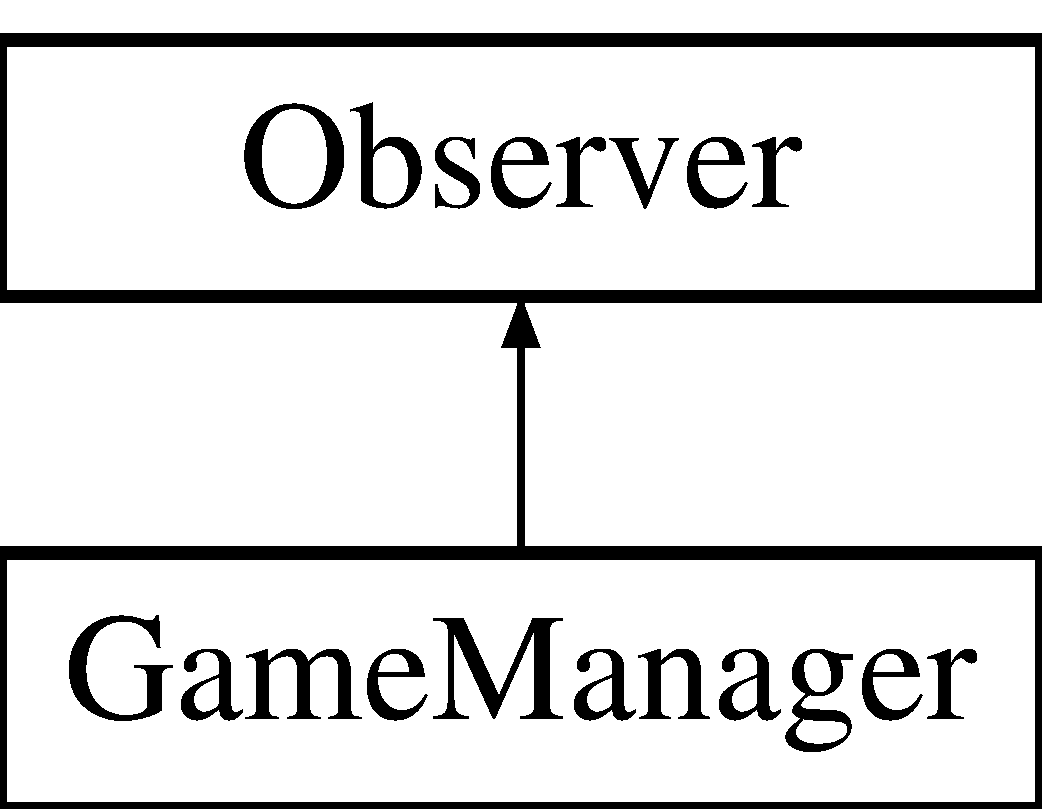
\includegraphics[height=2.000000cm]{class_game_manager}
\end{center}
\end{figure}
\subsection*{Public Member Functions}
\begin{DoxyCompactItemize}
\item 
\hypertarget{class_game_manager_a8ca3e8bfd80b9c5637a279ba0a779859}{{\bfseries Game\-Manager} (\hyperlink{class_crazy_river_ride}{Crazy\-River\-Ride} $\ast$)}\label{class_game_manager_a8ca3e8bfd80b9c5637a279ba0a779859}

\item 
\hypertarget{class_game_manager_a46f13cda874d5146c65db959d44607c8}{void {\bfseries run\-A\-Game} ()}\label{class_game_manager_a46f13cda874d5146c65db959d44607c8}

\item 
\hypertarget{class_game_manager_a24ac94e016dc0ad440faa7b88ee31840}{int {\bfseries get\-X\-Axis} ()}\label{class_game_manager_a24ac94e016dc0ad440faa7b88ee31840}

\item 
\hypertarget{class_game_manager_abe4ae648e6067c8bd19a1d020c292560}{int {\bfseries get\-Y\-Axis} ()}\label{class_game_manager_abe4ae648e6067c8bd19a1d020c292560}

\item 
\hypertarget{class_game_manager_a6b43e9e166a906789e4b4aa134218994}{bool {\bfseries shoot} ()}\label{class_game_manager_a6b43e9e166a906789e4b4aa134218994}

\item 
\hypertarget{class_game_manager_a91a7e823176e56f32ca0b582592d7b02}{bool {\bfseries pause} ()}\label{class_game_manager_a91a7e823176e56f32ca0b582592d7b02}

\item 
\hypertarget{class_game_manager_a0c03dfd4e0fd50e0d9159da2b3d15342}{void {\bfseries select} (int Map)}\label{class_game_manager_a0c03dfd4e0fd50e0d9159da2b3d15342}

\item 
void \hyperlink{class_game_manager_abcc7beda88f37957ab1c0711de030a45}{update} (google\-::protobuf\-::\-Message $\ast$p\-Message)
\begin{DoxyCompactList}\small\item\em Recibe un mensaje mediante el uso de protocol buffers de google Recibe el protocolo, y lo decodifica con la implementacion necesaria que se le de al la clase que sobrescriba este metodo virtual. \end{DoxyCompactList}\end{DoxyCompactItemize}


\subsection{Member Function Documentation}
\hypertarget{class_game_manager_abcc7beda88f37957ab1c0711de030a45}{\index{Game\-Manager@{Game\-Manager}!update@{update}}
\index{update@{update}!GameManager@{Game\-Manager}}
\subsubsection[{update}]{\setlength{\rightskip}{0pt plus 5cm}void Game\-Manager\-::update (
\begin{DoxyParamCaption}
\item[{google\-::protobuf\-::\-Message $\ast$}]{p\-Message}
\end{DoxyParamCaption}
)\hspace{0.3cm}{\ttfamily [virtual]}}}\label{class_game_manager_abcc7beda88f37957ab1c0711de030a45}


Recibe un mensaje mediante el uso de protocol buffers de google Recibe el protocolo, y lo decodifica con la implementacion necesaria que se le de al la clase que sobrescriba este metodo virtual. 


\begin{DoxyParams}{Parameters}
{\em p\-Message} & Es el mensaje recibido que es parte de los protocol buffers de google \\
\hline
\end{DoxyParams}


Implements \hyperlink{class_observer_a7204fd48ae9f9c2f39ea7e165740c451}{Observer}.



The documentation for this class was generated from the following files\-:\begin{DoxyCompactItemize}
\item 
gamemanager.\-h\item 
gamemanager.\-cpp\end{DoxyCompactItemize}

\hypertarget{class_game_map}{\section{Game\-Map Class Reference}
\label{class_game_map}\index{Game\-Map@{Game\-Map}}
}


Es el mapa del nivel.  




{\ttfamily \#include $<$gamemap.\-h$>$}

Inheritance diagram for Game\-Map\-:\begin{figure}[H]
\begin{center}
\leavevmode
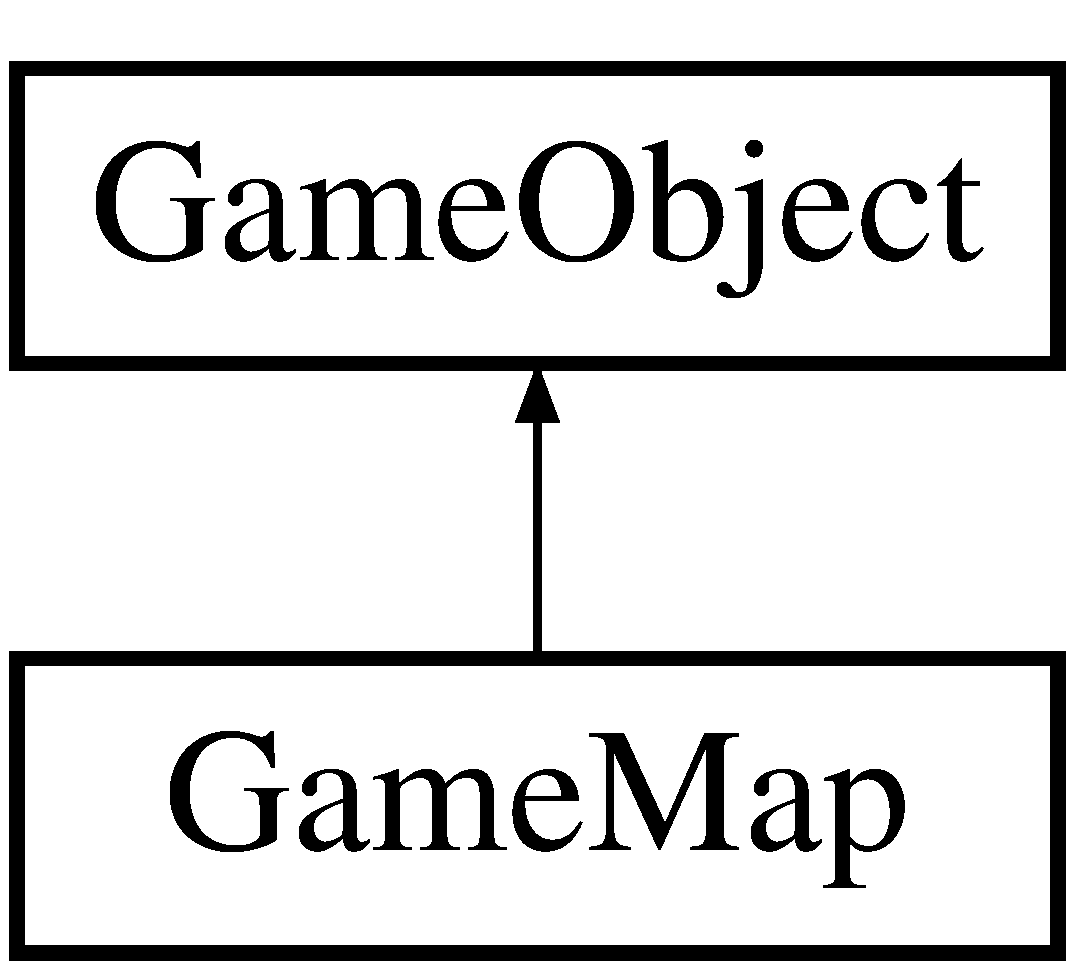
\includegraphics[height=2.000000cm]{class_game_map}
\end{center}
\end{figure}
\subsection*{Public Member Functions}
\begin{DoxyCompactItemize}
\item 
\hyperlink{class_game_map_aa62bdfa76f7c48dc6b384870491747c7}{Game\-Map} (Q\-Rect p\-Rect, int p\-Vy, int p\-Limit)
\begin{DoxyCompactList}\small\item\em Es el constructor de la clase, da un rectangulo que da la posicion y dimensiones del objeto, tambien la velocidad en el eje Y que se movera el objeto y un limite que le diga hasta que punto llegar en el eje Y. \end{DoxyCompactList}\item 
\hypertarget{class_game_map_a6497b5f848c5ac2945c0beabb896bead}{void \hyperlink{class_game_map_a6497b5f848c5ac2945c0beabb896bead}{update} ()}\label{class_game_map_a6497b5f848c5ac2945c0beabb896bead}

\begin{DoxyCompactList}\small\item\em Actualiza la posicion del mapa hasta llegar al limite impuesto. \end{DoxyCompactList}\end{DoxyCompactItemize}
\subsection*{Additional Inherited Members}


\subsection{Detailed Description}
Es el mapa del nivel. 

\subsection{Constructor \& Destructor Documentation}
\hypertarget{class_game_map_aa62bdfa76f7c48dc6b384870491747c7}{\index{Game\-Map@{Game\-Map}!Game\-Map@{Game\-Map}}
\index{Game\-Map@{Game\-Map}!GameMap@{Game\-Map}}
\subsubsection[{Game\-Map}]{\setlength{\rightskip}{0pt plus 5cm}Game\-Map\-::\-Game\-Map (
\begin{DoxyParamCaption}
\item[{Q\-Rect}]{p\-Rect, }
\item[{int}]{p\-Vy, }
\item[{int}]{p\-Limit}
\end{DoxyParamCaption}
)}}\label{class_game_map_aa62bdfa76f7c48dc6b384870491747c7}


Es el constructor de la clase, da un rectangulo que da la posicion y dimensiones del objeto, tambien la velocidad en el eje Y que se movera el objeto y un limite que le diga hasta que punto llegar en el eje Y. 


\begin{DoxyParams}{Parameters}
{\em p\-Rect} & contiene las dimensiones del objeto a crear \\
\hline
{\em p\-Vy} & es la velocidad en el eje Y \\
\hline
{\em p\-Limit} & es el limite hasta el cual se movera el objeto \\
\hline
\end{DoxyParams}


The documentation for this class was generated from the following files\-:\begin{DoxyCompactItemize}
\item 
logic/mapobjects/gamemap.\-h\item 
logic/mapobjects/gamemap.\-cpp\end{DoxyCompactItemize}

\hypertarget{class_game_menu}{\section{Game\-Menu Class Reference}
\label{class_game_menu}\index{Game\-Menu@{Game\-Menu}}
}


{\ttfamily \#include $<$Game\-Menu.\-pb.\-h$>$}

Inheritance diagram for Game\-Menu\-:\begin{figure}[H]
\begin{center}
\leavevmode
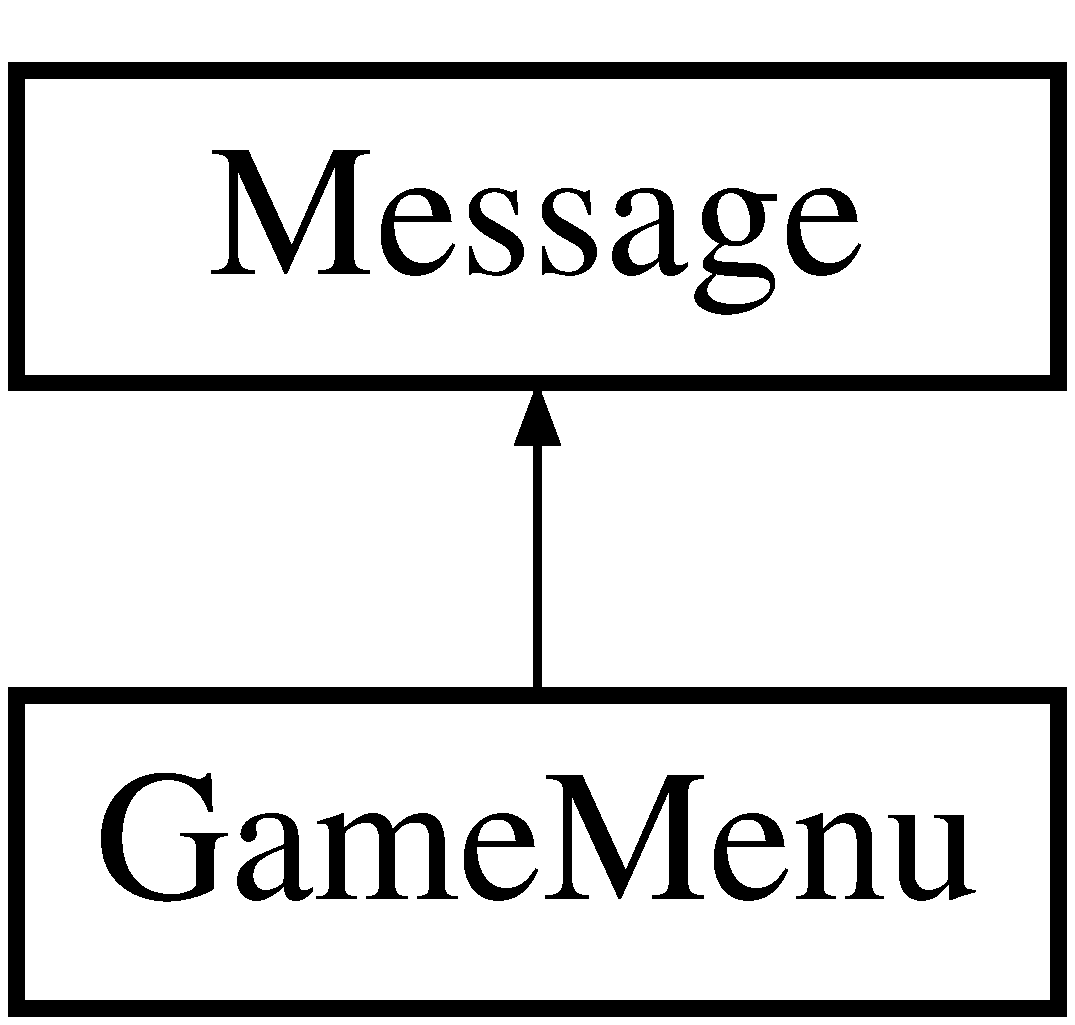
\includegraphics[height=2.000000cm]{class_game_menu}
\end{center}
\end{figure}
\subsection*{Public Member Functions}
\begin{DoxyCompactItemize}
\item 
\hyperlink{class_game_menu_ae31c50148abf655297a2a3eab53c15a3}{Game\-Menu} ()
\item 
virtual \hyperlink{class_game_menu_a70ac0e31f882993f09eb1bdbdd352a56}{$\sim$\-Game\-Menu} ()
\item 
\hyperlink{class_game_menu_a0a1b44357508921c4f6edee476abb7b1}{Game\-Menu} (const \hyperlink{class_game_menu}{Game\-Menu} \&from)
\item 
\hyperlink{class_game_menu}{Game\-Menu} \& \hyperlink{class_game_menu_aaaf4f50a1d43e387811424fb4b09f93e}{operator=} (const \hyperlink{class_game_menu}{Game\-Menu} \&from)
\item 
const \\*
\-::google\-::protobuf\-::\-Unknown\-Field\-Set \& \hyperlink{class_game_menu_a1eaa869160e0897331da0ec3c015fec6}{unknown\-\_\-fields} () const 
\item 
inline\-::google\-::protobuf\-::\-Unknown\-Field\-Set $\ast$ \hyperlink{class_game_menu_a4092f328998bb9659d48903db1243b07}{mutable\-\_\-unknown\-\_\-fields} ()
\item 
void \hyperlink{class_game_menu_a8ecb2f60b010cbf56bf1f1c1756fd4cf}{Swap} (\hyperlink{class_game_menu}{Game\-Menu} $\ast$other)
\item 
\hyperlink{class_game_menu}{Game\-Menu} $\ast$ \hyperlink{class_game_menu_a44324114e8f5f3497fbff764ffbaec66}{New} () const 
\item 
\hyperlink{class_game_menu}{Game\-Menu} $\ast$ \hyperlink{class_game_menu_aa42d2be609f8e769b721b39d7857f1ea}{New} (\-::google\-::protobuf\-::\-Arena $\ast$arena) const 
\item 
void \hyperlink{class_game_menu_a13d4e96e0878e9bc0f848bcc4a5c9775}{Copy\-From} (const \-::google\-::protobuf\-::\-Message \&from)
\item 
void \hyperlink{class_game_menu_a82f6ca7995e5bc16aa40e02cc35226f3}{Merge\-From} (const \-::google\-::protobuf\-::\-Message \&from)
\item 
void \hyperlink{class_game_menu_a785301f9d4c73689d7aa3115680e870e}{Copy\-From} (const \hyperlink{class_game_menu}{Game\-Menu} \&from)
\item 
void \hyperlink{class_game_menu_a8ebfff6cb9a723430dbfdd50903bc411}{Merge\-From} (const \hyperlink{class_game_menu}{Game\-Menu} \&from)
\item 
void \hyperlink{class_game_menu_acb122483cb8b5048efd1852bbfba056d}{Clear} ()
\item 
bool \hyperlink{class_game_menu_aa915693f815cf5daf04471cedfb856e5}{Is\-Initialized} () const 
\item 
int \hyperlink{class_game_menu_a02d5db82aef1cc4952c969d49e708ecb}{Byte\-Size} () const 
\item 
bool \hyperlink{class_game_menu_af9f1ba343e861e93883b97e91ab8b223}{Merge\-Partial\-From\-Coded\-Stream} (\-::google\-::protobuf\-::io\-::\-Coded\-Input\-Stream $\ast$input)
\item 
void \hyperlink{class_game_menu_ad8286d01deedb8e7d8be6a538d2ec3d4}{Serialize\-With\-Cached\-Sizes} (\-::google\-::protobuf\-::io\-::\-Coded\-Output\-Stream $\ast$output) const 
\item 
\-::google\-::protobuf\-::uint8 $\ast$ \hyperlink{class_game_menu_a43ac30c609cbcda0c80ef5882bac6b11}{Serialize\-With\-Cached\-Sizes\-To\-Array} (\-::google\-::protobuf\-::uint8 $\ast$output) const 
\item 
int \hyperlink{class_game_menu_a0c6c6b9b554509c67943a875eca1ee2f}{Get\-Cached\-Size} () const 
\item 
\-::google\-::protobuf\-::\-Metadata \hyperlink{class_game_menu_aac2d5a1cf8855aa80e4e72a53397b396}{Get\-Metadata} () const 
\item 
bool \hyperlink{class_game_menu_a0f1d555993fae1f4bb4610de51082169}{has\-\_\-buttonx} () const 
\item 
void \hyperlink{class_game_menu_a200f23f0a7b562455ba4e0fe418bd751}{clear\-\_\-buttonx} ()
\item 
inline\-::google\-::protobuf\-::int32 \hyperlink{class_game_menu_aea17fc7a000f75a96a4b1b26dfd76778}{buttonx} () const 
\item 
void \hyperlink{class_game_menu_a5fdecafb0ddc1119cca7111d796ca4b1}{set\-\_\-buttonx} (\-::google\-::protobuf\-::int32 value)
\item 
bool \hyperlink{class_game_menu_aa081759411b7f4df72b589ca69fc00b2}{has\-\_\-buttony} () const 
\item 
void \hyperlink{class_game_menu_afc095342e5c7f7231d70eb99c522bbfb}{clear\-\_\-buttony} ()
\item 
inline\-::google\-::protobuf\-::int32 \hyperlink{class_game_menu_aa680aff8de83627d3659f5354fdbfa8e}{buttony} () const 
\item 
void \hyperlink{class_game_menu_a5012a247ded2ab16c4d0e9760aecbee1}{set\-\_\-buttony} (\-::google\-::protobuf\-::int32 value)
\item 
bool \hyperlink{class_game_menu_af2a429e3dea81aefb27e507b34a6b450}{has\-\_\-buttonwidth} () const 
\item 
void \hyperlink{class_game_menu_a530076caa9483b223c89ba806f1ab996}{clear\-\_\-buttonwidth} ()
\item 
inline\-::google\-::protobuf\-::int32 \hyperlink{class_game_menu_a129d9ca0747a44437f0bb7181cd92fba}{buttonwidth} () const 
\item 
void \hyperlink{class_game_menu_a56aa7ceffcc93eb338206c82127b7f62}{set\-\_\-buttonwidth} (\-::google\-::protobuf\-::int32 value)
\item 
bool \hyperlink{class_game_menu_a5f109f581d3786a458d156260a2acb84}{has\-\_\-buttonheight} () const 
\item 
void \hyperlink{class_game_menu_a9d6ca35aac1c8addef27536bb63c691f}{clear\-\_\-buttonheight} ()
\item 
inline\-::google\-::protobuf\-::int32 \hyperlink{class_game_menu_a0d6c040f3b994ab558e2d2dbc11fcef0}{buttonheight} () const 
\item 
void \hyperlink{class_game_menu_ae1aa83ed7078237a0914bcd24964d446}{set\-\_\-buttonheight} (\-::google\-::protobuf\-::int32 value)
\item 
bool \hyperlink{class_game_menu_a28214c378a1acdefc8d85d8dd360939b}{has\-\_\-buttonactive} () const 
\item 
void \hyperlink{class_game_menu_a95b04ee1a6c6677bb225c3797d9d8061}{clear\-\_\-buttonactive} ()
\item 
bool \hyperlink{class_game_menu_ac53f3dde12a642d330498c33ecb1386f}{buttonactive} () const 
\item 
void \hyperlink{class_game_menu_af3fe74b06fabc19c5df391917ace597b}{set\-\_\-buttonactive} (bool value)
\end{DoxyCompactItemize}
\subsection*{Static Public Member Functions}
\begin{DoxyCompactItemize}
\item 
static const \\*
\-::google\-::protobuf\-::\-Descriptor $\ast$ \hyperlink{class_game_menu_a9a58d7e3eed9e066adc5b407a36ba292}{descriptor} ()
\item 
static const \hyperlink{class_game_menu}{Game\-Menu} \& \hyperlink{class_game_menu_afeb4b86432ba501c5c1627410b0848ad}{default\-\_\-instance} ()
\end{DoxyCompactItemize}
\subsection*{Static Public Attributes}
\begin{DoxyCompactItemize}
\item 
static const int \hyperlink{class_game_menu_abe2fdf1262f6916050a5bcca9222486a}{k\-Button\-X\-Field\-Number} = 1
\item 
static const int \hyperlink{class_game_menu_ae3096491e0598302630a930f29280b6c}{k\-Button\-Y\-Field\-Number} = 2
\item 
static const int \hyperlink{class_game_menu_a9005124c7b657675f79d175b758bbfd3}{k\-Button\-Width\-Field\-Number} = 3
\item 
static const int \hyperlink{class_game_menu_aa4c6206a7f24f81750af4160e871d5ba}{k\-Button\-Height\-Field\-Number} = 4
\item 
static const int \hyperlink{class_game_menu_abf765ea4cffd8e765a7643700214676a}{k\-Button\-Active\-Field\-Number} = 5
\end{DoxyCompactItemize}
\subsection*{Friends}
\begin{DoxyCompactItemize}
\item 
void \hyperlink{class_game_menu_adab92a19f73074ecd5246095c9c960b4}{protobuf\-\_\-\-Add\-Desc\-\_\-\-Game\-Menu\-\_\-2eproto} ()
\item 
void \hyperlink{class_game_menu_a510004e21d3b33f46c1dd043a543e933}{protobuf\-\_\-\-Assign\-Desc\-\_\-\-Game\-Menu\-\_\-2eproto} ()
\item 
void \hyperlink{class_game_menu_aa91d1c6168e6662eb7667848e4cef2c3}{protobuf\-\_\-\-Shutdown\-File\-\_\-\-Game\-Menu\-\_\-2eproto} ()
\end{DoxyCompactItemize}


\subsection{Constructor \& Destructor Documentation}
\hypertarget{class_game_menu_ae31c50148abf655297a2a3eab53c15a3}{\index{Game\-Menu@{Game\-Menu}!Game\-Menu@{Game\-Menu}}
\index{Game\-Menu@{Game\-Menu}!GameMenu@{Game\-Menu}}
\subsubsection[{Game\-Menu}]{\setlength{\rightskip}{0pt plus 5cm}Game\-Menu\-::\-Game\-Menu (
\begin{DoxyParamCaption}
{}
\end{DoxyParamCaption}
)}}\label{class_game_menu_ae31c50148abf655297a2a3eab53c15a3}
\hypertarget{class_game_menu_a70ac0e31f882993f09eb1bdbdd352a56}{\index{Game\-Menu@{Game\-Menu}!$\sim$\-Game\-Menu@{$\sim$\-Game\-Menu}}
\index{$\sim$\-Game\-Menu@{$\sim$\-Game\-Menu}!GameMenu@{Game\-Menu}}
\subsubsection[{$\sim$\-Game\-Menu}]{\setlength{\rightskip}{0pt plus 5cm}Game\-Menu\-::$\sim$\-Game\-Menu (
\begin{DoxyParamCaption}
{}
\end{DoxyParamCaption}
)\hspace{0.3cm}{\ttfamily [virtual]}}}\label{class_game_menu_a70ac0e31f882993f09eb1bdbdd352a56}
\hypertarget{class_game_menu_a0a1b44357508921c4f6edee476abb7b1}{\index{Game\-Menu@{Game\-Menu}!Game\-Menu@{Game\-Menu}}
\index{Game\-Menu@{Game\-Menu}!GameMenu@{Game\-Menu}}
\subsubsection[{Game\-Menu}]{\setlength{\rightskip}{0pt plus 5cm}Game\-Menu\-::\-Game\-Menu (
\begin{DoxyParamCaption}
\item[{const {\bf Game\-Menu} \&}]{from}
\end{DoxyParamCaption}
)}}\label{class_game_menu_a0a1b44357508921c4f6edee476abb7b1}


\subsection{Member Function Documentation}
\hypertarget{class_game_menu_ac53f3dde12a642d330498c33ecb1386f}{\index{Game\-Menu@{Game\-Menu}!buttonactive@{buttonactive}}
\index{buttonactive@{buttonactive}!GameMenu@{Game\-Menu}}
\subsubsection[{buttonactive}]{\setlength{\rightskip}{0pt plus 5cm}bool Game\-Menu\-::buttonactive (
\begin{DoxyParamCaption}
{}
\end{DoxyParamCaption}
) const\hspace{0.3cm}{\ttfamily [inline]}}}\label{class_game_menu_ac53f3dde12a642d330498c33ecb1386f}
\hypertarget{class_game_menu_a0d6c040f3b994ab558e2d2dbc11fcef0}{\index{Game\-Menu@{Game\-Menu}!buttonheight@{buttonheight}}
\index{buttonheight@{buttonheight}!GameMenu@{Game\-Menu}}
\subsubsection[{buttonheight}]{\setlength{\rightskip}{0pt plus 5cm}google\-::protobuf\-::int32 Game\-Menu\-::buttonheight (
\begin{DoxyParamCaption}
{}
\end{DoxyParamCaption}
) const\hspace{0.3cm}{\ttfamily [inline]}}}\label{class_game_menu_a0d6c040f3b994ab558e2d2dbc11fcef0}
\hypertarget{class_game_menu_a129d9ca0747a44437f0bb7181cd92fba}{\index{Game\-Menu@{Game\-Menu}!buttonwidth@{buttonwidth}}
\index{buttonwidth@{buttonwidth}!GameMenu@{Game\-Menu}}
\subsubsection[{buttonwidth}]{\setlength{\rightskip}{0pt plus 5cm}google\-::protobuf\-::int32 Game\-Menu\-::buttonwidth (
\begin{DoxyParamCaption}
{}
\end{DoxyParamCaption}
) const\hspace{0.3cm}{\ttfamily [inline]}}}\label{class_game_menu_a129d9ca0747a44437f0bb7181cd92fba}
\hypertarget{class_game_menu_aea17fc7a000f75a96a4b1b26dfd76778}{\index{Game\-Menu@{Game\-Menu}!buttonx@{buttonx}}
\index{buttonx@{buttonx}!GameMenu@{Game\-Menu}}
\subsubsection[{buttonx}]{\setlength{\rightskip}{0pt plus 5cm}google\-::protobuf\-::int32 Game\-Menu\-::buttonx (
\begin{DoxyParamCaption}
{}
\end{DoxyParamCaption}
) const\hspace{0.3cm}{\ttfamily [inline]}}}\label{class_game_menu_aea17fc7a000f75a96a4b1b26dfd76778}
\hypertarget{class_game_menu_aa680aff8de83627d3659f5354fdbfa8e}{\index{Game\-Menu@{Game\-Menu}!buttony@{buttony}}
\index{buttony@{buttony}!GameMenu@{Game\-Menu}}
\subsubsection[{buttony}]{\setlength{\rightskip}{0pt plus 5cm}google\-::protobuf\-::int32 Game\-Menu\-::buttony (
\begin{DoxyParamCaption}
{}
\end{DoxyParamCaption}
) const\hspace{0.3cm}{\ttfamily [inline]}}}\label{class_game_menu_aa680aff8de83627d3659f5354fdbfa8e}
\hypertarget{class_game_menu_a02d5db82aef1cc4952c969d49e708ecb}{\index{Game\-Menu@{Game\-Menu}!Byte\-Size@{Byte\-Size}}
\index{Byte\-Size@{Byte\-Size}!GameMenu@{Game\-Menu}}
\subsubsection[{Byte\-Size}]{\setlength{\rightskip}{0pt plus 5cm}int Game\-Menu\-::\-Byte\-Size (
\begin{DoxyParamCaption}
{}
\end{DoxyParamCaption}
) const}}\label{class_game_menu_a02d5db82aef1cc4952c969d49e708ecb}
\hypertarget{class_game_menu_acb122483cb8b5048efd1852bbfba056d}{\index{Game\-Menu@{Game\-Menu}!Clear@{Clear}}
\index{Clear@{Clear}!GameMenu@{Game\-Menu}}
\subsubsection[{Clear}]{\setlength{\rightskip}{0pt plus 5cm}void Game\-Menu\-::\-Clear (
\begin{DoxyParamCaption}
{}
\end{DoxyParamCaption}
)}}\label{class_game_menu_acb122483cb8b5048efd1852bbfba056d}
\hypertarget{class_game_menu_a95b04ee1a6c6677bb225c3797d9d8061}{\index{Game\-Menu@{Game\-Menu}!clear\-\_\-buttonactive@{clear\-\_\-buttonactive}}
\index{clear\-\_\-buttonactive@{clear\-\_\-buttonactive}!GameMenu@{Game\-Menu}}
\subsubsection[{clear\-\_\-buttonactive}]{\setlength{\rightskip}{0pt plus 5cm}void Game\-Menu\-::clear\-\_\-buttonactive (
\begin{DoxyParamCaption}
{}
\end{DoxyParamCaption}
)\hspace{0.3cm}{\ttfamily [inline]}}}\label{class_game_menu_a95b04ee1a6c6677bb225c3797d9d8061}
\hypertarget{class_game_menu_a9d6ca35aac1c8addef27536bb63c691f}{\index{Game\-Menu@{Game\-Menu}!clear\-\_\-buttonheight@{clear\-\_\-buttonheight}}
\index{clear\-\_\-buttonheight@{clear\-\_\-buttonheight}!GameMenu@{Game\-Menu}}
\subsubsection[{clear\-\_\-buttonheight}]{\setlength{\rightskip}{0pt plus 5cm}void Game\-Menu\-::clear\-\_\-buttonheight (
\begin{DoxyParamCaption}
{}
\end{DoxyParamCaption}
)\hspace{0.3cm}{\ttfamily [inline]}}}\label{class_game_menu_a9d6ca35aac1c8addef27536bb63c691f}
\hypertarget{class_game_menu_a530076caa9483b223c89ba806f1ab996}{\index{Game\-Menu@{Game\-Menu}!clear\-\_\-buttonwidth@{clear\-\_\-buttonwidth}}
\index{clear\-\_\-buttonwidth@{clear\-\_\-buttonwidth}!GameMenu@{Game\-Menu}}
\subsubsection[{clear\-\_\-buttonwidth}]{\setlength{\rightskip}{0pt plus 5cm}void Game\-Menu\-::clear\-\_\-buttonwidth (
\begin{DoxyParamCaption}
{}
\end{DoxyParamCaption}
)\hspace{0.3cm}{\ttfamily [inline]}}}\label{class_game_menu_a530076caa9483b223c89ba806f1ab996}
\hypertarget{class_game_menu_a200f23f0a7b562455ba4e0fe418bd751}{\index{Game\-Menu@{Game\-Menu}!clear\-\_\-buttonx@{clear\-\_\-buttonx}}
\index{clear\-\_\-buttonx@{clear\-\_\-buttonx}!GameMenu@{Game\-Menu}}
\subsubsection[{clear\-\_\-buttonx}]{\setlength{\rightskip}{0pt plus 5cm}void Game\-Menu\-::clear\-\_\-buttonx (
\begin{DoxyParamCaption}
{}
\end{DoxyParamCaption}
)\hspace{0.3cm}{\ttfamily [inline]}}}\label{class_game_menu_a200f23f0a7b562455ba4e0fe418bd751}
\hypertarget{class_game_menu_afc095342e5c7f7231d70eb99c522bbfb}{\index{Game\-Menu@{Game\-Menu}!clear\-\_\-buttony@{clear\-\_\-buttony}}
\index{clear\-\_\-buttony@{clear\-\_\-buttony}!GameMenu@{Game\-Menu}}
\subsubsection[{clear\-\_\-buttony}]{\setlength{\rightskip}{0pt plus 5cm}void Game\-Menu\-::clear\-\_\-buttony (
\begin{DoxyParamCaption}
{}
\end{DoxyParamCaption}
)\hspace{0.3cm}{\ttfamily [inline]}}}\label{class_game_menu_afc095342e5c7f7231d70eb99c522bbfb}
\hypertarget{class_game_menu_a13d4e96e0878e9bc0f848bcc4a5c9775}{\index{Game\-Menu@{Game\-Menu}!Copy\-From@{Copy\-From}}
\index{Copy\-From@{Copy\-From}!GameMenu@{Game\-Menu}}
\subsubsection[{Copy\-From}]{\setlength{\rightskip}{0pt plus 5cm}void Game\-Menu\-::\-Copy\-From (
\begin{DoxyParamCaption}
\item[{const \-::google\-::protobuf\-::\-Message \&}]{from}
\end{DoxyParamCaption}
)}}\label{class_game_menu_a13d4e96e0878e9bc0f848bcc4a5c9775}
\hypertarget{class_game_menu_a785301f9d4c73689d7aa3115680e870e}{\index{Game\-Menu@{Game\-Menu}!Copy\-From@{Copy\-From}}
\index{Copy\-From@{Copy\-From}!GameMenu@{Game\-Menu}}
\subsubsection[{Copy\-From}]{\setlength{\rightskip}{0pt plus 5cm}void Game\-Menu\-::\-Copy\-From (
\begin{DoxyParamCaption}
\item[{const {\bf Game\-Menu} \&}]{from}
\end{DoxyParamCaption}
)}}\label{class_game_menu_a785301f9d4c73689d7aa3115680e870e}
\hypertarget{class_game_menu_afeb4b86432ba501c5c1627410b0848ad}{\index{Game\-Menu@{Game\-Menu}!default\-\_\-instance@{default\-\_\-instance}}
\index{default\-\_\-instance@{default\-\_\-instance}!GameMenu@{Game\-Menu}}
\subsubsection[{default\-\_\-instance}]{\setlength{\rightskip}{0pt plus 5cm}const {\bf Game\-Menu} \& Game\-Menu\-::default\-\_\-instance (
\begin{DoxyParamCaption}
{}
\end{DoxyParamCaption}
)\hspace{0.3cm}{\ttfamily [static]}}}\label{class_game_menu_afeb4b86432ba501c5c1627410b0848ad}
\hypertarget{class_game_menu_a9a58d7e3eed9e066adc5b407a36ba292}{\index{Game\-Menu@{Game\-Menu}!descriptor@{descriptor}}
\index{descriptor@{descriptor}!GameMenu@{Game\-Menu}}
\subsubsection[{descriptor}]{\setlength{\rightskip}{0pt plus 5cm}const \-::google\-::protobuf\-::\-Descriptor $\ast$ Game\-Menu\-::descriptor (
\begin{DoxyParamCaption}
{}
\end{DoxyParamCaption}
)\hspace{0.3cm}{\ttfamily [static]}}}\label{class_game_menu_a9a58d7e3eed9e066adc5b407a36ba292}
\hypertarget{class_game_menu_a0c6c6b9b554509c67943a875eca1ee2f}{\index{Game\-Menu@{Game\-Menu}!Get\-Cached\-Size@{Get\-Cached\-Size}}
\index{Get\-Cached\-Size@{Get\-Cached\-Size}!GameMenu@{Game\-Menu}}
\subsubsection[{Get\-Cached\-Size}]{\setlength{\rightskip}{0pt plus 5cm}int Game\-Menu\-::\-Get\-Cached\-Size (
\begin{DoxyParamCaption}
{}
\end{DoxyParamCaption}
) const\hspace{0.3cm}{\ttfamily [inline]}}}\label{class_game_menu_a0c6c6b9b554509c67943a875eca1ee2f}
\hypertarget{class_game_menu_aac2d5a1cf8855aa80e4e72a53397b396}{\index{Game\-Menu@{Game\-Menu}!Get\-Metadata@{Get\-Metadata}}
\index{Get\-Metadata@{Get\-Metadata}!GameMenu@{Game\-Menu}}
\subsubsection[{Get\-Metadata}]{\setlength{\rightskip}{0pt plus 5cm}google\-::protobuf\-::\-Metadata Game\-Menu\-::\-Get\-Metadata (
\begin{DoxyParamCaption}
{}
\end{DoxyParamCaption}
) const}}\label{class_game_menu_aac2d5a1cf8855aa80e4e72a53397b396}
\hypertarget{class_game_menu_a28214c378a1acdefc8d85d8dd360939b}{\index{Game\-Menu@{Game\-Menu}!has\-\_\-buttonactive@{has\-\_\-buttonactive}}
\index{has\-\_\-buttonactive@{has\-\_\-buttonactive}!GameMenu@{Game\-Menu}}
\subsubsection[{has\-\_\-buttonactive}]{\setlength{\rightskip}{0pt plus 5cm}bool Game\-Menu\-::has\-\_\-buttonactive (
\begin{DoxyParamCaption}
{}
\end{DoxyParamCaption}
) const\hspace{0.3cm}{\ttfamily [inline]}}}\label{class_game_menu_a28214c378a1acdefc8d85d8dd360939b}
\hypertarget{class_game_menu_a5f109f581d3786a458d156260a2acb84}{\index{Game\-Menu@{Game\-Menu}!has\-\_\-buttonheight@{has\-\_\-buttonheight}}
\index{has\-\_\-buttonheight@{has\-\_\-buttonheight}!GameMenu@{Game\-Menu}}
\subsubsection[{has\-\_\-buttonheight}]{\setlength{\rightskip}{0pt plus 5cm}bool Game\-Menu\-::has\-\_\-buttonheight (
\begin{DoxyParamCaption}
{}
\end{DoxyParamCaption}
) const\hspace{0.3cm}{\ttfamily [inline]}}}\label{class_game_menu_a5f109f581d3786a458d156260a2acb84}
\hypertarget{class_game_menu_af2a429e3dea81aefb27e507b34a6b450}{\index{Game\-Menu@{Game\-Menu}!has\-\_\-buttonwidth@{has\-\_\-buttonwidth}}
\index{has\-\_\-buttonwidth@{has\-\_\-buttonwidth}!GameMenu@{Game\-Menu}}
\subsubsection[{has\-\_\-buttonwidth}]{\setlength{\rightskip}{0pt plus 5cm}bool Game\-Menu\-::has\-\_\-buttonwidth (
\begin{DoxyParamCaption}
{}
\end{DoxyParamCaption}
) const\hspace{0.3cm}{\ttfamily [inline]}}}\label{class_game_menu_af2a429e3dea81aefb27e507b34a6b450}
\hypertarget{class_game_menu_a0f1d555993fae1f4bb4610de51082169}{\index{Game\-Menu@{Game\-Menu}!has\-\_\-buttonx@{has\-\_\-buttonx}}
\index{has\-\_\-buttonx@{has\-\_\-buttonx}!GameMenu@{Game\-Menu}}
\subsubsection[{has\-\_\-buttonx}]{\setlength{\rightskip}{0pt plus 5cm}bool Game\-Menu\-::has\-\_\-buttonx (
\begin{DoxyParamCaption}
{}
\end{DoxyParamCaption}
) const\hspace{0.3cm}{\ttfamily [inline]}}}\label{class_game_menu_a0f1d555993fae1f4bb4610de51082169}
\hypertarget{class_game_menu_aa081759411b7f4df72b589ca69fc00b2}{\index{Game\-Menu@{Game\-Menu}!has\-\_\-buttony@{has\-\_\-buttony}}
\index{has\-\_\-buttony@{has\-\_\-buttony}!GameMenu@{Game\-Menu}}
\subsubsection[{has\-\_\-buttony}]{\setlength{\rightskip}{0pt plus 5cm}bool Game\-Menu\-::has\-\_\-buttony (
\begin{DoxyParamCaption}
{}
\end{DoxyParamCaption}
) const\hspace{0.3cm}{\ttfamily [inline]}}}\label{class_game_menu_aa081759411b7f4df72b589ca69fc00b2}
\hypertarget{class_game_menu_aa915693f815cf5daf04471cedfb856e5}{\index{Game\-Menu@{Game\-Menu}!Is\-Initialized@{Is\-Initialized}}
\index{Is\-Initialized@{Is\-Initialized}!GameMenu@{Game\-Menu}}
\subsubsection[{Is\-Initialized}]{\setlength{\rightskip}{0pt plus 5cm}bool Game\-Menu\-::\-Is\-Initialized (
\begin{DoxyParamCaption}
{}
\end{DoxyParamCaption}
) const}}\label{class_game_menu_aa915693f815cf5daf04471cedfb856e5}
\hypertarget{class_game_menu_a82f6ca7995e5bc16aa40e02cc35226f3}{\index{Game\-Menu@{Game\-Menu}!Merge\-From@{Merge\-From}}
\index{Merge\-From@{Merge\-From}!GameMenu@{Game\-Menu}}
\subsubsection[{Merge\-From}]{\setlength{\rightskip}{0pt plus 5cm}void Game\-Menu\-::\-Merge\-From (
\begin{DoxyParamCaption}
\item[{const \-::google\-::protobuf\-::\-Message \&}]{from}
\end{DoxyParamCaption}
)}}\label{class_game_menu_a82f6ca7995e5bc16aa40e02cc35226f3}
\hypertarget{class_game_menu_a8ebfff6cb9a723430dbfdd50903bc411}{\index{Game\-Menu@{Game\-Menu}!Merge\-From@{Merge\-From}}
\index{Merge\-From@{Merge\-From}!GameMenu@{Game\-Menu}}
\subsubsection[{Merge\-From}]{\setlength{\rightskip}{0pt plus 5cm}void Game\-Menu\-::\-Merge\-From (
\begin{DoxyParamCaption}
\item[{const {\bf Game\-Menu} \&}]{from}
\end{DoxyParamCaption}
)}}\label{class_game_menu_a8ebfff6cb9a723430dbfdd50903bc411}
\hypertarget{class_game_menu_af9f1ba343e861e93883b97e91ab8b223}{\index{Game\-Menu@{Game\-Menu}!Merge\-Partial\-From\-Coded\-Stream@{Merge\-Partial\-From\-Coded\-Stream}}
\index{Merge\-Partial\-From\-Coded\-Stream@{Merge\-Partial\-From\-Coded\-Stream}!GameMenu@{Game\-Menu}}
\subsubsection[{Merge\-Partial\-From\-Coded\-Stream}]{\setlength{\rightskip}{0pt plus 5cm}bool Game\-Menu\-::\-Merge\-Partial\-From\-Coded\-Stream (
\begin{DoxyParamCaption}
\item[{\-::google\-::protobuf\-::io\-::\-Coded\-Input\-Stream $\ast$}]{input}
\end{DoxyParamCaption}
)}}\label{class_game_menu_af9f1ba343e861e93883b97e91ab8b223}
\hypertarget{class_game_menu_a4092f328998bb9659d48903db1243b07}{\index{Game\-Menu@{Game\-Menu}!mutable\-\_\-unknown\-\_\-fields@{mutable\-\_\-unknown\-\_\-fields}}
\index{mutable\-\_\-unknown\-\_\-fields@{mutable\-\_\-unknown\-\_\-fields}!GameMenu@{Game\-Menu}}
\subsubsection[{mutable\-\_\-unknown\-\_\-fields}]{\setlength{\rightskip}{0pt plus 5cm}inline \-::google\-::protobuf\-::\-Unknown\-Field\-Set$\ast$ Game\-Menu\-::mutable\-\_\-unknown\-\_\-fields (
\begin{DoxyParamCaption}
{}
\end{DoxyParamCaption}
)\hspace{0.3cm}{\ttfamily [inline]}}}\label{class_game_menu_a4092f328998bb9659d48903db1243b07}
\hypertarget{class_game_menu_a44324114e8f5f3497fbff764ffbaec66}{\index{Game\-Menu@{Game\-Menu}!New@{New}}
\index{New@{New}!GameMenu@{Game\-Menu}}
\subsubsection[{New}]{\setlength{\rightskip}{0pt plus 5cm}{\bf Game\-Menu}$\ast$ Game\-Menu\-::\-New (
\begin{DoxyParamCaption}
{}
\end{DoxyParamCaption}
) const\hspace{0.3cm}{\ttfamily [inline]}}}\label{class_game_menu_a44324114e8f5f3497fbff764ffbaec66}
\hypertarget{class_game_menu_aa42d2be609f8e769b721b39d7857f1ea}{\index{Game\-Menu@{Game\-Menu}!New@{New}}
\index{New@{New}!GameMenu@{Game\-Menu}}
\subsubsection[{New}]{\setlength{\rightskip}{0pt plus 5cm}{\bf Game\-Menu} $\ast$ Game\-Menu\-::\-New (
\begin{DoxyParamCaption}
\item[{\-::google\-::protobuf\-::\-Arena $\ast$}]{arena}
\end{DoxyParamCaption}
) const}}\label{class_game_menu_aa42d2be609f8e769b721b39d7857f1ea}
\hypertarget{class_game_menu_aaaf4f50a1d43e387811424fb4b09f93e}{\index{Game\-Menu@{Game\-Menu}!operator=@{operator=}}
\index{operator=@{operator=}!GameMenu@{Game\-Menu}}
\subsubsection[{operator=}]{\setlength{\rightskip}{0pt plus 5cm}{\bf Game\-Menu}\& Game\-Menu\-::operator= (
\begin{DoxyParamCaption}
\item[{const {\bf Game\-Menu} \&}]{from}
\end{DoxyParamCaption}
)\hspace{0.3cm}{\ttfamily [inline]}}}\label{class_game_menu_aaaf4f50a1d43e387811424fb4b09f93e}
\hypertarget{class_game_menu_ad8286d01deedb8e7d8be6a538d2ec3d4}{\index{Game\-Menu@{Game\-Menu}!Serialize\-With\-Cached\-Sizes@{Serialize\-With\-Cached\-Sizes}}
\index{Serialize\-With\-Cached\-Sizes@{Serialize\-With\-Cached\-Sizes}!GameMenu@{Game\-Menu}}
\subsubsection[{Serialize\-With\-Cached\-Sizes}]{\setlength{\rightskip}{0pt plus 5cm}void Game\-Menu\-::\-Serialize\-With\-Cached\-Sizes (
\begin{DoxyParamCaption}
\item[{\-::google\-::protobuf\-::io\-::\-Coded\-Output\-Stream $\ast$}]{output}
\end{DoxyParamCaption}
) const}}\label{class_game_menu_ad8286d01deedb8e7d8be6a538d2ec3d4}
\hypertarget{class_game_menu_a43ac30c609cbcda0c80ef5882bac6b11}{\index{Game\-Menu@{Game\-Menu}!Serialize\-With\-Cached\-Sizes\-To\-Array@{Serialize\-With\-Cached\-Sizes\-To\-Array}}
\index{Serialize\-With\-Cached\-Sizes\-To\-Array@{Serialize\-With\-Cached\-Sizes\-To\-Array}!GameMenu@{Game\-Menu}}
\subsubsection[{Serialize\-With\-Cached\-Sizes\-To\-Array}]{\setlength{\rightskip}{0pt plus 5cm}google\-::protobuf\-::uint8 $\ast$ Game\-Menu\-::\-Serialize\-With\-Cached\-Sizes\-To\-Array (
\begin{DoxyParamCaption}
\item[{\-::google\-::protobuf\-::uint8 $\ast$}]{output}
\end{DoxyParamCaption}
) const}}\label{class_game_menu_a43ac30c609cbcda0c80ef5882bac6b11}
\hypertarget{class_game_menu_af3fe74b06fabc19c5df391917ace597b}{\index{Game\-Menu@{Game\-Menu}!set\-\_\-buttonactive@{set\-\_\-buttonactive}}
\index{set\-\_\-buttonactive@{set\-\_\-buttonactive}!GameMenu@{Game\-Menu}}
\subsubsection[{set\-\_\-buttonactive}]{\setlength{\rightskip}{0pt plus 5cm}void Game\-Menu\-::set\-\_\-buttonactive (
\begin{DoxyParamCaption}
\item[{bool}]{value}
\end{DoxyParamCaption}
)\hspace{0.3cm}{\ttfamily [inline]}}}\label{class_game_menu_af3fe74b06fabc19c5df391917ace597b}
\hypertarget{class_game_menu_ae1aa83ed7078237a0914bcd24964d446}{\index{Game\-Menu@{Game\-Menu}!set\-\_\-buttonheight@{set\-\_\-buttonheight}}
\index{set\-\_\-buttonheight@{set\-\_\-buttonheight}!GameMenu@{Game\-Menu}}
\subsubsection[{set\-\_\-buttonheight}]{\setlength{\rightskip}{0pt plus 5cm}void Game\-Menu\-::set\-\_\-buttonheight (
\begin{DoxyParamCaption}
\item[{\-::google\-::protobuf\-::int32}]{value}
\end{DoxyParamCaption}
)\hspace{0.3cm}{\ttfamily [inline]}}}\label{class_game_menu_ae1aa83ed7078237a0914bcd24964d446}
\hypertarget{class_game_menu_a56aa7ceffcc93eb338206c82127b7f62}{\index{Game\-Menu@{Game\-Menu}!set\-\_\-buttonwidth@{set\-\_\-buttonwidth}}
\index{set\-\_\-buttonwidth@{set\-\_\-buttonwidth}!GameMenu@{Game\-Menu}}
\subsubsection[{set\-\_\-buttonwidth}]{\setlength{\rightskip}{0pt plus 5cm}void Game\-Menu\-::set\-\_\-buttonwidth (
\begin{DoxyParamCaption}
\item[{\-::google\-::protobuf\-::int32}]{value}
\end{DoxyParamCaption}
)\hspace{0.3cm}{\ttfamily [inline]}}}\label{class_game_menu_a56aa7ceffcc93eb338206c82127b7f62}
\hypertarget{class_game_menu_a5fdecafb0ddc1119cca7111d796ca4b1}{\index{Game\-Menu@{Game\-Menu}!set\-\_\-buttonx@{set\-\_\-buttonx}}
\index{set\-\_\-buttonx@{set\-\_\-buttonx}!GameMenu@{Game\-Menu}}
\subsubsection[{set\-\_\-buttonx}]{\setlength{\rightskip}{0pt plus 5cm}void Game\-Menu\-::set\-\_\-buttonx (
\begin{DoxyParamCaption}
\item[{\-::google\-::protobuf\-::int32}]{value}
\end{DoxyParamCaption}
)\hspace{0.3cm}{\ttfamily [inline]}}}\label{class_game_menu_a5fdecafb0ddc1119cca7111d796ca4b1}
\hypertarget{class_game_menu_a5012a247ded2ab16c4d0e9760aecbee1}{\index{Game\-Menu@{Game\-Menu}!set\-\_\-buttony@{set\-\_\-buttony}}
\index{set\-\_\-buttony@{set\-\_\-buttony}!GameMenu@{Game\-Menu}}
\subsubsection[{set\-\_\-buttony}]{\setlength{\rightskip}{0pt plus 5cm}void Game\-Menu\-::set\-\_\-buttony (
\begin{DoxyParamCaption}
\item[{\-::google\-::protobuf\-::int32}]{value}
\end{DoxyParamCaption}
)\hspace{0.3cm}{\ttfamily [inline]}}}\label{class_game_menu_a5012a247ded2ab16c4d0e9760aecbee1}
\hypertarget{class_game_menu_a8ecb2f60b010cbf56bf1f1c1756fd4cf}{\index{Game\-Menu@{Game\-Menu}!Swap@{Swap}}
\index{Swap@{Swap}!GameMenu@{Game\-Menu}}
\subsubsection[{Swap}]{\setlength{\rightskip}{0pt plus 5cm}void Game\-Menu\-::\-Swap (
\begin{DoxyParamCaption}
\item[{{\bf Game\-Menu} $\ast$}]{other}
\end{DoxyParamCaption}
)}}\label{class_game_menu_a8ecb2f60b010cbf56bf1f1c1756fd4cf}
\hypertarget{class_game_menu_a1eaa869160e0897331da0ec3c015fec6}{\index{Game\-Menu@{Game\-Menu}!unknown\-\_\-fields@{unknown\-\_\-fields}}
\index{unknown\-\_\-fields@{unknown\-\_\-fields}!GameMenu@{Game\-Menu}}
\subsubsection[{unknown\-\_\-fields}]{\setlength{\rightskip}{0pt plus 5cm}const \-::google\-::protobuf\-::\-Unknown\-Field\-Set\& Game\-Menu\-::unknown\-\_\-fields (
\begin{DoxyParamCaption}
{}
\end{DoxyParamCaption}
) const\hspace{0.3cm}{\ttfamily [inline]}}}\label{class_game_menu_a1eaa869160e0897331da0ec3c015fec6}


\subsection{Friends And Related Function Documentation}
\hypertarget{class_game_menu_adab92a19f73074ecd5246095c9c960b4}{\index{Game\-Menu@{Game\-Menu}!protobuf\-\_\-\-Add\-Desc\-\_\-\-Game\-Menu\-\_\-2eproto@{protobuf\-\_\-\-Add\-Desc\-\_\-\-Game\-Menu\-\_\-2eproto}}
\index{protobuf\-\_\-\-Add\-Desc\-\_\-\-Game\-Menu\-\_\-2eproto@{protobuf\-\_\-\-Add\-Desc\-\_\-\-Game\-Menu\-\_\-2eproto}!GameMenu@{Game\-Menu}}
\subsubsection[{protobuf\-\_\-\-Add\-Desc\-\_\-\-Game\-Menu\-\_\-2eproto}]{\setlength{\rightskip}{0pt plus 5cm}void protobuf\-\_\-\-Add\-Desc\-\_\-\-Game\-Menu\-\_\-2eproto (
\begin{DoxyParamCaption}
{}
\end{DoxyParamCaption}
)\hspace{0.3cm}{\ttfamily [friend]}}}\label{class_game_menu_adab92a19f73074ecd5246095c9c960b4}
\hypertarget{class_game_menu_a510004e21d3b33f46c1dd043a543e933}{\index{Game\-Menu@{Game\-Menu}!protobuf\-\_\-\-Assign\-Desc\-\_\-\-Game\-Menu\-\_\-2eproto@{protobuf\-\_\-\-Assign\-Desc\-\_\-\-Game\-Menu\-\_\-2eproto}}
\index{protobuf\-\_\-\-Assign\-Desc\-\_\-\-Game\-Menu\-\_\-2eproto@{protobuf\-\_\-\-Assign\-Desc\-\_\-\-Game\-Menu\-\_\-2eproto}!GameMenu@{Game\-Menu}}
\subsubsection[{protobuf\-\_\-\-Assign\-Desc\-\_\-\-Game\-Menu\-\_\-2eproto}]{\setlength{\rightskip}{0pt plus 5cm}void protobuf\-\_\-\-Assign\-Desc\-\_\-\-Game\-Menu\-\_\-2eproto (
\begin{DoxyParamCaption}
{}
\end{DoxyParamCaption}
)\hspace{0.3cm}{\ttfamily [friend]}}}\label{class_game_menu_a510004e21d3b33f46c1dd043a543e933}
\hypertarget{class_game_menu_aa91d1c6168e6662eb7667848e4cef2c3}{\index{Game\-Menu@{Game\-Menu}!protobuf\-\_\-\-Shutdown\-File\-\_\-\-Game\-Menu\-\_\-2eproto@{protobuf\-\_\-\-Shutdown\-File\-\_\-\-Game\-Menu\-\_\-2eproto}}
\index{protobuf\-\_\-\-Shutdown\-File\-\_\-\-Game\-Menu\-\_\-2eproto@{protobuf\-\_\-\-Shutdown\-File\-\_\-\-Game\-Menu\-\_\-2eproto}!GameMenu@{Game\-Menu}}
\subsubsection[{protobuf\-\_\-\-Shutdown\-File\-\_\-\-Game\-Menu\-\_\-2eproto}]{\setlength{\rightskip}{0pt plus 5cm}void protobuf\-\_\-\-Shutdown\-File\-\_\-\-Game\-Menu\-\_\-2eproto (
\begin{DoxyParamCaption}
{}
\end{DoxyParamCaption}
)\hspace{0.3cm}{\ttfamily [friend]}}}\label{class_game_menu_aa91d1c6168e6662eb7667848e4cef2c3}


\subsection{Member Data Documentation}
\hypertarget{class_game_menu_abf765ea4cffd8e765a7643700214676a}{\index{Game\-Menu@{Game\-Menu}!k\-Button\-Active\-Field\-Number@{k\-Button\-Active\-Field\-Number}}
\index{k\-Button\-Active\-Field\-Number@{k\-Button\-Active\-Field\-Number}!GameMenu@{Game\-Menu}}
\subsubsection[{k\-Button\-Active\-Field\-Number}]{\setlength{\rightskip}{0pt plus 5cm}const int Game\-Menu\-::k\-Button\-Active\-Field\-Number = 5\hspace{0.3cm}{\ttfamily [static]}}}\label{class_game_menu_abf765ea4cffd8e765a7643700214676a}
\hypertarget{class_game_menu_aa4c6206a7f24f81750af4160e871d5ba}{\index{Game\-Menu@{Game\-Menu}!k\-Button\-Height\-Field\-Number@{k\-Button\-Height\-Field\-Number}}
\index{k\-Button\-Height\-Field\-Number@{k\-Button\-Height\-Field\-Number}!GameMenu@{Game\-Menu}}
\subsubsection[{k\-Button\-Height\-Field\-Number}]{\setlength{\rightskip}{0pt plus 5cm}const int Game\-Menu\-::k\-Button\-Height\-Field\-Number = 4\hspace{0.3cm}{\ttfamily [static]}}}\label{class_game_menu_aa4c6206a7f24f81750af4160e871d5ba}
\hypertarget{class_game_menu_a9005124c7b657675f79d175b758bbfd3}{\index{Game\-Menu@{Game\-Menu}!k\-Button\-Width\-Field\-Number@{k\-Button\-Width\-Field\-Number}}
\index{k\-Button\-Width\-Field\-Number@{k\-Button\-Width\-Field\-Number}!GameMenu@{Game\-Menu}}
\subsubsection[{k\-Button\-Width\-Field\-Number}]{\setlength{\rightskip}{0pt plus 5cm}const int Game\-Menu\-::k\-Button\-Width\-Field\-Number = 3\hspace{0.3cm}{\ttfamily [static]}}}\label{class_game_menu_a9005124c7b657675f79d175b758bbfd3}
\hypertarget{class_game_menu_abe2fdf1262f6916050a5bcca9222486a}{\index{Game\-Menu@{Game\-Menu}!k\-Button\-X\-Field\-Number@{k\-Button\-X\-Field\-Number}}
\index{k\-Button\-X\-Field\-Number@{k\-Button\-X\-Field\-Number}!GameMenu@{Game\-Menu}}
\subsubsection[{k\-Button\-X\-Field\-Number}]{\setlength{\rightskip}{0pt plus 5cm}const int Game\-Menu\-::k\-Button\-X\-Field\-Number = 1\hspace{0.3cm}{\ttfamily [static]}}}\label{class_game_menu_abe2fdf1262f6916050a5bcca9222486a}
\hypertarget{class_game_menu_ae3096491e0598302630a930f29280b6c}{\index{Game\-Menu@{Game\-Menu}!k\-Button\-Y\-Field\-Number@{k\-Button\-Y\-Field\-Number}}
\index{k\-Button\-Y\-Field\-Number@{k\-Button\-Y\-Field\-Number}!GameMenu@{Game\-Menu}}
\subsubsection[{k\-Button\-Y\-Field\-Number}]{\setlength{\rightskip}{0pt plus 5cm}const int Game\-Menu\-::k\-Button\-Y\-Field\-Number = 2\hspace{0.3cm}{\ttfamily [static]}}}\label{class_game_menu_ae3096491e0598302630a930f29280b6c}


The documentation for this class was generated from the following files\-:\begin{DoxyCompactItemize}
\item 
protobufmessage/\hyperlink{_game_menu_8pb_8h}{Game\-Menu.\-pb.\-h}\item 
protobufmessage/\hyperlink{_game_menu_8pb_8cc}{Game\-Menu.\-pb.\-cc}\end{DoxyCompactItemize}

\hypertarget{class_game_object}{\section{Game\-Object Class Reference}
\label{class_game_object}\index{Game\-Object@{Game\-Object}}
}


Es el objeto principal del programa contiene todas las abstracciones posibles y pensadas por los programadores que trabajaron en ella. El objetivo de esta clase es abstraer la mayoria de las operaciones basicas y comunes entre objetos que contengan rectangulos y deban verificar si colisionan, no olvidando la caracteristica basica de los objetos de este juego,, la tendencia a estar en movimiento, a ser D\-I\-N\-A\-M\-I\-C\-O\-S. De esta clase derivan un monton, y son pocas en comparacion a su utilidad.  




{\ttfamily \#include $<$gameobject.\-h$>$}

Inheritance diagram for Game\-Object\-:\begin{figure}[H]
\begin{center}
\leavevmode
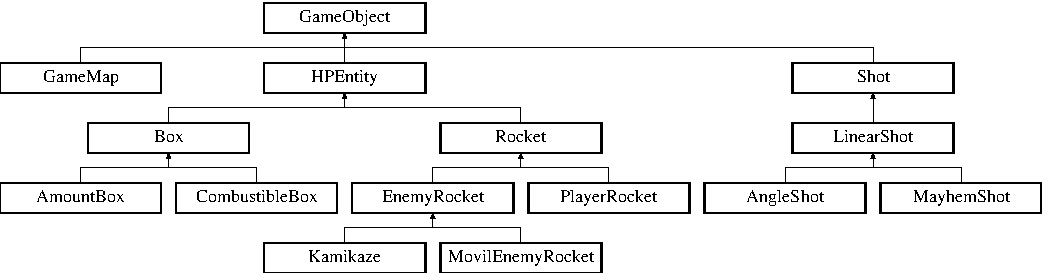
\includegraphics[height=3.674541cm]{class_game_object}
\end{center}
\end{figure}
\subsection*{Public Member Functions}
\begin{DoxyCompactItemize}
\item 
\hyperlink{class_game_object_a439d121ac13b4727d0bbb850e1ada980}{Game\-Object} (Q\-Rect p\-Rect)
\begin{DoxyCompactList}\small\item\em Es el constructor de la clase es encarga de asignar un rectangulo al objeto que se va a instanciar con este metodo. \end{DoxyCompactList}\item 
\hyperlink{class_game_object_aefff75a70a358b683a9e698b05abd3dd}{Game\-Object} (\hyperlink{class_game_object}{Game\-Object} \&go)
\begin{DoxyCompactList}\small\item\em Es el constructor de copia. \end{DoxyCompactList}\item 
virtual Q\-Rect \hyperlink{class_game_object_a529e5908a2c7a95fe3cd0f47958471b4}{get\-Rect} ()
\begin{DoxyCompactList}\small\item\em obtiene una copia del rectangulo contenido en esta clase \end{DoxyCompactList}\item 
virtual bool \hyperlink{class_game_object_a4d7f7506ab6fa6442367844cd8202fb6}{is\-Collide} (\hyperlink{class_game_object}{Game\-Object} $\ast$\-\_\-other\-Renderizable)
\begin{DoxyCompactList}\small\item\em Verifica si un \hyperlink{class_game_object}{Game\-Object} esta colisionando con otro. \end{DoxyCompactList}\item 
\hypertarget{class_game_object_ae83128d0e0efef691417779605ee037c}{virtual void \hyperlink{class_game_object_ae83128d0e0efef691417779605ee037c}{update} ()=0}\label{class_game_object_ae83128d0e0efef691417779605ee037c}

\begin{DoxyCompactList}\small\item\em Actualiza el objeto, es un metodo abstracto, y debe ser implementado por sus clases hijas. \end{DoxyCompactList}\item 
virtual string \hyperlink{class_game_object_a340e4594b8eafacc5bd6f7e390b43f53}{get\-Id} ()
\begin{DoxyCompactList}\small\item\em Obtiene el I\-D unico del objeto. \end{DoxyCompactList}\item 
virtual int \hyperlink{class_game_object_a2553f445dc1aa30defaa3bc0875927ba}{get\-Height} () const 
\begin{DoxyCompactList}\small\item\em obtiene el alto del objeto de juego \end{DoxyCompactList}\item 
virtual int \hyperlink{class_game_object_a3c6c20c513c069dc2cf6aee2649581b2}{get\-Width} () const 
\begin{DoxyCompactList}\small\item\em o¡obtiene el ancho del objeto de juego \end{DoxyCompactList}\item 
virtual int \hyperlink{class_game_object_a8f9c430b6cef5177a0a7f8649e749d10}{get\-X} () const 
\begin{DoxyCompactList}\small\item\em Obtiene la posicion en el eje X del objeto de juego. \end{DoxyCompactList}\item 
virtual int \hyperlink{class_game_object_a3ae8f58696691791813f0c58af6fffd8}{get\-Y} () const 
\begin{DoxyCompactList}\small\item\em Obtiene la posicion en el eje y del objeto de juego. \end{DoxyCompactList}\item 
\hypertarget{class_game_object_ab82dfdb656f9051c0587e6593b2dda97}{virtual \hyperlink{class_game_object_ab82dfdb656f9051c0587e6593b2dda97}{$\sim$\-Game\-Object} ()}\label{class_game_object_ab82dfdb656f9051c0587e6593b2dda97}

\begin{DoxyCompactList}\small\item\em Destructor de la clase. \end{DoxyCompactList}\end{DoxyCompactItemize}
\subsection*{Protected Member Functions}
\begin{DoxyCompactItemize}
\item 
void \hyperlink{class_game_object_ae8bb850eb78ebf34e764b8dbd3ea5fab}{move\-In\-Place} (int p\-X, int p\-Y)
\begin{DoxyCompactList}\small\item\em Se encarga de mover el objeto desde la direccion de donde esta, no se encarga de mover el objeto a un punto especifico, si no, de la posicion de la que se encuentra, moverlo lo que se desea en el eje y como en el x. \end{DoxyCompactList}\end{DoxyCompactItemize}
\subsection*{Protected Attributes}
\begin{DoxyCompactItemize}
\item 
Q\-Rect \hyperlink{class_game_object_a38a2dff83aae28ebffee5c4b833626a2}{\-\_\-\-Rectangle}
\item 
string \hyperlink{class_game_object_a74075bae5de6b22a17098e60964e676b}{\-\_\-\-Id}
\end{DoxyCompactItemize}
\subsection*{Static Protected Attributes}
\begin{DoxyCompactItemize}
\item 
static int \hyperlink{class_game_object_aeeec17db7fc77fe70148a9d6edd99ea4}{\-\_\-\-Serial} = 0
\end{DoxyCompactItemize}


\subsection{Detailed Description}
Es el objeto principal del programa contiene todas las abstracciones posibles y pensadas por los programadores que trabajaron en ella. El objetivo de esta clase es abstraer la mayoria de las operaciones basicas y comunes entre objetos que contengan rectangulos y deban verificar si colisionan, no olvidando la caracteristica basica de los objetos de este juego,, la tendencia a estar en movimiento, a ser D\-I\-N\-A\-M\-I\-C\-O\-S. De esta clase derivan un monton, y son pocas en comparacion a su utilidad. 

\subsection{Constructor \& Destructor Documentation}
\hypertarget{class_game_object_a439d121ac13b4727d0bbb850e1ada980}{\index{Game\-Object@{Game\-Object}!Game\-Object@{Game\-Object}}
\index{Game\-Object@{Game\-Object}!GameObject@{Game\-Object}}
\subsubsection[{Game\-Object}]{\setlength{\rightskip}{0pt plus 5cm}Game\-Object\-::\-Game\-Object (
\begin{DoxyParamCaption}
\item[{Q\-Rect}]{p\-Rect}
\end{DoxyParamCaption}
)}}\label{class_game_object_a439d121ac13b4727d0bbb850e1ada980}


Es el constructor de la clase es encarga de asignar un rectangulo al objeto que se va a instanciar con este metodo. 


\begin{DoxyParams}{Parameters}
{\em p\-Rect} & el rectangulo que desea asignarse al objeto que desea crearse con este constructor \\
\hline
\end{DoxyParams}
\hypertarget{class_game_object_aefff75a70a358b683a9e698b05abd3dd}{\index{Game\-Object@{Game\-Object}!Game\-Object@{Game\-Object}}
\index{Game\-Object@{Game\-Object}!GameObject@{Game\-Object}}
\subsubsection[{Game\-Object}]{\setlength{\rightskip}{0pt plus 5cm}Game\-Object\-::\-Game\-Object (
\begin{DoxyParamCaption}
\item[{{\bf Game\-Object} \&}]{go}
\end{DoxyParamCaption}
)}}\label{class_game_object_aefff75a70a358b683a9e698b05abd3dd}


Es el constructor de copia. 


\begin{DoxyParams}{Parameters}
{\em go} & es el objeto que desea copiarse \\
\hline
\end{DoxyParams}


\subsection{Member Function Documentation}
\hypertarget{class_game_object_a2553f445dc1aa30defaa3bc0875927ba}{\index{Game\-Object@{Game\-Object}!get\-Height@{get\-Height}}
\index{get\-Height@{get\-Height}!GameObject@{Game\-Object}}
\subsubsection[{get\-Height}]{\setlength{\rightskip}{0pt plus 5cm}int Game\-Object\-::get\-Height (
\begin{DoxyParamCaption}
{}
\end{DoxyParamCaption}
) const\hspace{0.3cm}{\ttfamily [virtual]}}}\label{class_game_object_a2553f445dc1aa30defaa3bc0875927ba}


obtiene el alto del objeto de juego 

\begin{DoxyReturn}{Returns}
int el alto del objeto del juego 
\end{DoxyReturn}
\hypertarget{class_game_object_a340e4594b8eafacc5bd6f7e390b43f53}{\index{Game\-Object@{Game\-Object}!get\-Id@{get\-Id}}
\index{get\-Id@{get\-Id}!GameObject@{Game\-Object}}
\subsubsection[{get\-Id}]{\setlength{\rightskip}{0pt plus 5cm}string Game\-Object\-::get\-Id (
\begin{DoxyParamCaption}
{}
\end{DoxyParamCaption}
)\hspace{0.3cm}{\ttfamily [virtual]}}}\label{class_game_object_a340e4594b8eafacc5bd6f7e390b43f53}


Obtiene el I\-D unico del objeto. 

\begin{DoxyReturn}{Returns}
string el id del objeto de juego 
\end{DoxyReturn}
\hypertarget{class_game_object_a529e5908a2c7a95fe3cd0f47958471b4}{\index{Game\-Object@{Game\-Object}!get\-Rect@{get\-Rect}}
\index{get\-Rect@{get\-Rect}!GameObject@{Game\-Object}}
\subsubsection[{get\-Rect}]{\setlength{\rightskip}{0pt plus 5cm}Q\-Rect Game\-Object\-::get\-Rect (
\begin{DoxyParamCaption}
{}
\end{DoxyParamCaption}
)\hspace{0.3cm}{\ttfamily [virtual]}}}\label{class_game_object_a529e5908a2c7a95fe3cd0f47958471b4}


obtiene una copia del rectangulo contenido en esta clase 

\begin{DoxyReturn}{Returns}
Q\-Rect el rectangulo del objeto 
\end{DoxyReturn}
\hypertarget{class_game_object_a3c6c20c513c069dc2cf6aee2649581b2}{\index{Game\-Object@{Game\-Object}!get\-Width@{get\-Width}}
\index{get\-Width@{get\-Width}!GameObject@{Game\-Object}}
\subsubsection[{get\-Width}]{\setlength{\rightskip}{0pt plus 5cm}int Game\-Object\-::get\-Width (
\begin{DoxyParamCaption}
{}
\end{DoxyParamCaption}
) const\hspace{0.3cm}{\ttfamily [virtual]}}}\label{class_game_object_a3c6c20c513c069dc2cf6aee2649581b2}


o¡obtiene el ancho del objeto de juego 

\begin{DoxyReturn}{Returns}
int el ancho del objeto de juego 
\end{DoxyReturn}
\hypertarget{class_game_object_a8f9c430b6cef5177a0a7f8649e749d10}{\index{Game\-Object@{Game\-Object}!get\-X@{get\-X}}
\index{get\-X@{get\-X}!GameObject@{Game\-Object}}
\subsubsection[{get\-X}]{\setlength{\rightskip}{0pt plus 5cm}int Game\-Object\-::get\-X (
\begin{DoxyParamCaption}
{}
\end{DoxyParamCaption}
) const\hspace{0.3cm}{\ttfamily [virtual]}}}\label{class_game_object_a8f9c430b6cef5177a0a7f8649e749d10}


Obtiene la posicion en el eje X del objeto de juego. 

\begin{DoxyReturn}{Returns}
int las posicion en x 
\end{DoxyReturn}
\hypertarget{class_game_object_a3ae8f58696691791813f0c58af6fffd8}{\index{Game\-Object@{Game\-Object}!get\-Y@{get\-Y}}
\index{get\-Y@{get\-Y}!GameObject@{Game\-Object}}
\subsubsection[{get\-Y}]{\setlength{\rightskip}{0pt plus 5cm}int Game\-Object\-::get\-Y (
\begin{DoxyParamCaption}
{}
\end{DoxyParamCaption}
) const\hspace{0.3cm}{\ttfamily [virtual]}}}\label{class_game_object_a3ae8f58696691791813f0c58af6fffd8}


Obtiene la posicion en el eje y del objeto de juego. 

\begin{DoxyReturn}{Returns}
int la posicion en el eje y 
\end{DoxyReturn}
\hypertarget{class_game_object_a4d7f7506ab6fa6442367844cd8202fb6}{\index{Game\-Object@{Game\-Object}!is\-Collide@{is\-Collide}}
\index{is\-Collide@{is\-Collide}!GameObject@{Game\-Object}}
\subsubsection[{is\-Collide}]{\setlength{\rightskip}{0pt plus 5cm}bool Game\-Object\-::is\-Collide (
\begin{DoxyParamCaption}
\item[{{\bf Game\-Object} $\ast$}]{\-\_\-other\-Renderizable}
\end{DoxyParamCaption}
)\hspace{0.3cm}{\ttfamily [virtual]}}}\label{class_game_object_a4d7f7506ab6fa6442367844cd8202fb6}


Verifica si un \hyperlink{class_game_object}{Game\-Object} esta colisionando con otro. 


\begin{DoxyParams}{Parameters}
{\em \-\_\-other\-Renderizable} & el otro objeto para verificar que se colisione \\
\hline
\end{DoxyParams}
\begin{DoxyReturn}{Returns}
true si colisionan 
\end{DoxyReturn}


Reimplemented in \hyperlink{class_linear_shot_a5f74863ef2fe90a8e524945737029e0a}{Linear\-Shot}.

\hypertarget{class_game_object_ae8bb850eb78ebf34e764b8dbd3ea5fab}{\index{Game\-Object@{Game\-Object}!move\-In\-Place@{move\-In\-Place}}
\index{move\-In\-Place@{move\-In\-Place}!GameObject@{Game\-Object}}
\subsubsection[{move\-In\-Place}]{\setlength{\rightskip}{0pt plus 5cm}void Game\-Object\-::move\-In\-Place (
\begin{DoxyParamCaption}
\item[{int}]{p\-X, }
\item[{int}]{p\-Y}
\end{DoxyParamCaption}
)\hspace{0.3cm}{\ttfamily [protected]}}}\label{class_game_object_ae8bb850eb78ebf34e764b8dbd3ea5fab}


Se encarga de mover el objeto desde la direccion de donde esta, no se encarga de mover el objeto a un punto especifico, si no, de la posicion de la que se encuentra, moverlo lo que se desea en el eje y como en el x. 


\begin{DoxyParams}{Parameters}
{\em p\-X} & es la cantidad de pixeles que se quiere mover el objeto en el eje x desde la posicion en la que se encuentra \\
\hline
{\em p\-Y} & es la cantidad de pixeles que se quiere mover el objeto en el eje y desde la posicion en la que se encuentra \\
\hline
\end{DoxyParams}


\subsection{Member Data Documentation}
\hypertarget{class_game_object_a74075bae5de6b22a17098e60964e676b}{\index{Game\-Object@{Game\-Object}!\-\_\-\-Id@{\-\_\-\-Id}}
\index{\-\_\-\-Id@{\-\_\-\-Id}!GameObject@{Game\-Object}}
\subsubsection[{\-\_\-\-Id}]{\setlength{\rightskip}{0pt plus 5cm}string Game\-Object\-::\-\_\-\-Id\hspace{0.3cm}{\ttfamily [protected]}}}\label{class_game_object_a74075bae5de6b22a17098e60964e676b}
T\-O\-D\-O es el identificador unico de cada objeto se pensaba usar en versiones pasadas, ahora es obsoleto \hypertarget{class_game_object_a38a2dff83aae28ebffee5c4b833626a2}{\index{Game\-Object@{Game\-Object}!\-\_\-\-Rectangle@{\-\_\-\-Rectangle}}
\index{\-\_\-\-Rectangle@{\-\_\-\-Rectangle}!GameObject@{Game\-Object}}
\subsubsection[{\-\_\-\-Rectangle}]{\setlength{\rightskip}{0pt plus 5cm}Q\-Rect Game\-Object\-::\-\_\-\-Rectangle\hspace{0.3cm}{\ttfamily [protected]}}}\label{class_game_object_a38a2dff83aae28ebffee5c4b833626a2}
T\-O\-D\-O Es el rectangulo que posee las coordenadas y dimensiones del objeto \hypertarget{class_game_object_aeeec17db7fc77fe70148a9d6edd99ea4}{\index{Game\-Object@{Game\-Object}!\-\_\-\-Serial@{\-\_\-\-Serial}}
\index{\-\_\-\-Serial@{\-\_\-\-Serial}!GameObject@{Game\-Object}}
\subsubsection[{\-\_\-\-Serial}]{\setlength{\rightskip}{0pt plus 5cm}int Game\-Object\-::\-\_\-\-Serial = 0\hspace{0.3cm}{\ttfamily [static]}, {\ttfamily [protected]}}}\label{class_game_object_aeeec17db7fc77fe70148a9d6edd99ea4}
T\-O\-D\-O 

The documentation for this class was generated from the following files\-:\begin{DoxyCompactItemize}
\item 
logic/mapobjects/gameobject.\-h\item 
logic/mapobjects/gameobject.\-cpp\end{DoxyCompactItemize}

\hypertarget{class_game_object_notify}{\section{Game\-Object\-Notify Class Reference}
\label{class_game_object_notify}\index{Game\-Object\-Notify@{Game\-Object\-Notify}}
}


{\ttfamily \#include $<$Game\-Object\-Notify.\-pb.\-h$>$}

Inheritance diagram for Game\-Object\-Notify\-:\begin{figure}[H]
\begin{center}
\leavevmode
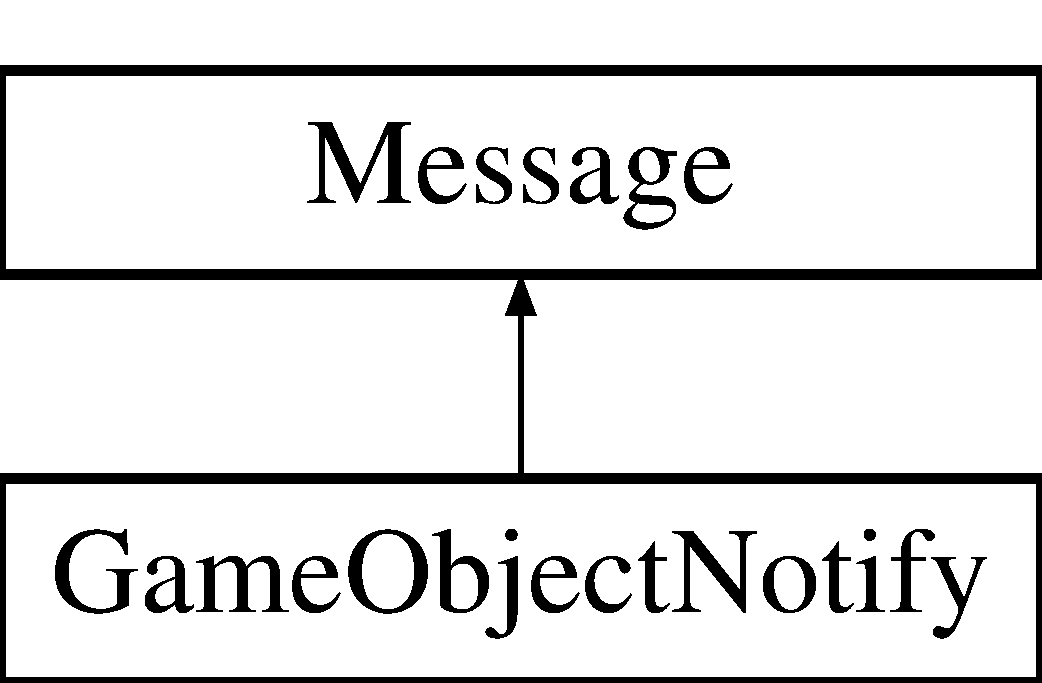
\includegraphics[height=2.000000cm]{class_game_object_notify}
\end{center}
\end{figure}
\subsection*{Public Member Functions}
\begin{DoxyCompactItemize}
\item 
\hyperlink{class_game_object_notify_a3e6824a087bec1744cfc9fba71fbc3f1}{Game\-Object\-Notify} ()
\item 
virtual \hyperlink{class_game_object_notify_ae85e7bbaea50075595a69c5d78bb2811}{$\sim$\-Game\-Object\-Notify} ()
\item 
\hyperlink{class_game_object_notify_af06e2a782b8a599555ba395d3dec804f}{Game\-Object\-Notify} (const \hyperlink{class_game_object_notify}{Game\-Object\-Notify} \&from)
\item 
\hyperlink{class_game_object_notify}{Game\-Object\-Notify} \& \hyperlink{class_game_object_notify_ab1951c4b4e75f13c67646b445d526863}{operator=} (const \hyperlink{class_game_object_notify}{Game\-Object\-Notify} \&from)
\item 
const \\*
\-::google\-::protobuf\-::\-Unknown\-Field\-Set \& \hyperlink{class_game_object_notify_a8d2d6ccfc91cd27a05fcc9e97534cc50}{unknown\-\_\-fields} () const 
\item 
inline\-::google\-::protobuf\-::\-Unknown\-Field\-Set $\ast$ \hyperlink{class_game_object_notify_aafb21632fce77e41d8b2e9cf723df223}{mutable\-\_\-unknown\-\_\-fields} ()
\item 
void \hyperlink{class_game_object_notify_ab4cd82478c332a44e03c65249a717ebb}{Swap} (\hyperlink{class_game_object_notify}{Game\-Object\-Notify} $\ast$other)
\item 
\hyperlink{class_game_object_notify}{Game\-Object\-Notify} $\ast$ \hyperlink{class_game_object_notify_ab6e37de74e40079ef7b30f0291b93220}{New} () const 
\item 
\hyperlink{class_game_object_notify}{Game\-Object\-Notify} $\ast$ \hyperlink{class_game_object_notify_a338c9aaf5767581cf0ccbe566a22cd03}{New} (\-::google\-::protobuf\-::\-Arena $\ast$arena) const 
\item 
void \hyperlink{class_game_object_notify_a45a598344fda5647816ed6bba5b94c95}{Copy\-From} (const \-::google\-::protobuf\-::\-Message \&from)
\item 
void \hyperlink{class_game_object_notify_af2604fb22741c6304ee689d8de537075}{Merge\-From} (const \-::google\-::protobuf\-::\-Message \&from)
\item 
void \hyperlink{class_game_object_notify_af163bd4f2834c44583ad22ff80c5fa34}{Copy\-From} (const \hyperlink{class_game_object_notify}{Game\-Object\-Notify} \&from)
\item 
void \hyperlink{class_game_object_notify_a185bd7dc2f070e9e98fa12158d160dad}{Merge\-From} (const \hyperlink{class_game_object_notify}{Game\-Object\-Notify} \&from)
\item 
void \hyperlink{class_game_object_notify_a7f116fae390b87419a829241f6ea0197}{Clear} ()
\item 
bool \hyperlink{class_game_object_notify_a4a821d184827fdafccab3a697dc666c6}{Is\-Initialized} () const 
\item 
int \hyperlink{class_game_object_notify_a63635477dec6ef117cc2e20e9a9f55dd}{Byte\-Size} () const 
\item 
bool \hyperlink{class_game_object_notify_aaa19ace0d7b2ce545036315be7509456}{Merge\-Partial\-From\-Coded\-Stream} (\-::google\-::protobuf\-::io\-::\-Coded\-Input\-Stream $\ast$input)
\item 
void \hyperlink{class_game_object_notify_a7995608370fc8c5c03a9358a9efbfa85}{Serialize\-With\-Cached\-Sizes} (\-::google\-::protobuf\-::io\-::\-Coded\-Output\-Stream $\ast$output) const 
\item 
\-::google\-::protobuf\-::uint8 $\ast$ \hyperlink{class_game_object_notify_ab5cc1ecedbad464ce4c41eecb433578a}{Serialize\-With\-Cached\-Sizes\-To\-Array} (\-::google\-::protobuf\-::uint8 $\ast$output) const 
\item 
int \hyperlink{class_game_object_notify_a5acae24a360fd54d2d7205008062ecc5}{Get\-Cached\-Size} () const 
\item 
\-::google\-::protobuf\-::\-Metadata \hyperlink{class_game_object_notify_acd92d4fc01971fb1ee172cf5a31e62e0}{Get\-Metadata} () const 
\item 
bool \hyperlink{class_game_object_notify_a986b979c2aa32d4e32c252b669a9b77f}{has\-\_\-type} () const 
\item 
void \hyperlink{class_game_object_notify_af14051d1680998ba235723a1ce0fd2b6}{clear\-\_\-type} ()
\item 
inline\-::google\-::protobuf\-::int32 \hyperlink{class_game_object_notify_ae8d17de08521388d76f137110050bf13}{type} () const 
\item 
void \hyperlink{class_game_object_notify_a7fe38481f8de7d9692856779d01b92db}{set\-\_\-type} (\-::google\-::protobuf\-::int32 value)
\item 
bool \hyperlink{class_game_object_notify_a716aa746890feeaeddfdafc070416c56}{has\-\_\-x} () const 
\item 
void \hyperlink{class_game_object_notify_a64d8f47b2e78c603f6d0133480a869ec}{clear\-\_\-x} ()
\item 
inline\-::google\-::protobuf\-::int32 \hyperlink{class_game_object_notify_a29d7c1745284cc5b78956cc316376738}{x} () const 
\item 
void \hyperlink{class_game_object_notify_a998082bfecd2c4cb76c84065a65b8e2a}{set\-\_\-x} (\-::google\-::protobuf\-::int32 value)
\item 
bool \hyperlink{class_game_object_notify_a74513aef5aceea983df19a445352ccb9}{has\-\_\-y} () const 
\item 
void \hyperlink{class_game_object_notify_a6f7b06cf818edf08ea2d5c09fd769853}{clear\-\_\-y} ()
\item 
inline\-::google\-::protobuf\-::int32 \hyperlink{class_game_object_notify_aefde9869ad1e80659b4951398a460f57}{y} () const 
\item 
void \hyperlink{class_game_object_notify_a9b2ee70f340e34b895d5c58bbda1967a}{set\-\_\-y} (\-::google\-::protobuf\-::int32 value)
\item 
bool \hyperlink{class_game_object_notify_ac571c7cc6962f862a30b3ae8f61432c7}{has\-\_\-width} () const 
\item 
void \hyperlink{class_game_object_notify_abd5293bda07b2a790702c7e039d7115a}{clear\-\_\-width} ()
\item 
inline\-::google\-::protobuf\-::int32 \hyperlink{class_game_object_notify_a53e65ba98c60fada040ccb9b1691bc32}{width} () const 
\item 
void \hyperlink{class_game_object_notify_adc1447c2773f943ff80233f89af49bc6}{set\-\_\-width} (\-::google\-::protobuf\-::int32 value)
\item 
bool \hyperlink{class_game_object_notify_acb2fd8a9f778bb0c6dc559c757e7c326}{has\-\_\-height} () const 
\item 
void \hyperlink{class_game_object_notify_ace893d2ef8f4a322762f85a2ed674ec1}{clear\-\_\-height} ()
\item 
inline\-::google\-::protobuf\-::int32 \hyperlink{class_game_object_notify_a7af70a9bc8ddcbe3bed697f772a324fc}{height} () const 
\item 
void \hyperlink{class_game_object_notify_a4075dd8cd90d521540217508f9864503}{set\-\_\-height} (\-::google\-::protobuf\-::int32 value)
\end{DoxyCompactItemize}
\subsection*{Static Public Member Functions}
\begin{DoxyCompactItemize}
\item 
static const \\*
\-::google\-::protobuf\-::\-Descriptor $\ast$ \hyperlink{class_game_object_notify_aaca556ce856cfffb364b49e244fe84d6}{descriptor} ()
\item 
static const \hyperlink{class_game_object_notify}{Game\-Object\-Notify} \& \hyperlink{class_game_object_notify_a1638acf0c0d50781c9c6290c78621080}{default\-\_\-instance} ()
\end{DoxyCompactItemize}
\subsection*{Static Public Attributes}
\begin{DoxyCompactItemize}
\item 
static const int \hyperlink{class_game_object_notify_a1686fae6e717999f7a4a3c883336ae5d}{k\-T\-Y\-P\-E\-Field\-Number} = 1
\item 
static const int \hyperlink{class_game_object_notify_a433cdc06e51abce278f247ff3a046608}{k\-X\-Field\-Number} = 2
\item 
static const int \hyperlink{class_game_object_notify_a4750c0b42b3b9515597e0d6665245f56}{k\-Y\-Field\-Number} = 3
\item 
static const int \hyperlink{class_game_object_notify_a5462ed3aee65d02ae60fe9a2de05a849}{k\-Width\-Field\-Number} = 4
\item 
static const int \hyperlink{class_game_object_notify_a15142be03ab21831b8f54cd346a409a2}{k\-Height\-Field\-Number} = 5
\end{DoxyCompactItemize}
\subsection*{Friends}
\begin{DoxyCompactItemize}
\item 
void \hyperlink{class_game_object_notify_ad39fab9cb60a70367567c18bd3667614}{protobuf\-\_\-\-Add\-Desc\-\_\-\-Game\-Object\-Notify\-\_\-2eproto} ()
\item 
void \hyperlink{class_game_object_notify_abfcb28a9131368bf7de1e6967278aeb4}{protobuf\-\_\-\-Assign\-Desc\-\_\-\-Game\-Object\-Notify\-\_\-2eproto} ()
\item 
void \hyperlink{class_game_object_notify_a849952bd288bb23b66755e3f6fb3f8b6}{protobuf\-\_\-\-Shutdown\-File\-\_\-\-Game\-Object\-Notify\-\_\-2eproto} ()
\end{DoxyCompactItemize}


\subsection{Constructor \& Destructor Documentation}
\hypertarget{class_game_object_notify_a3e6824a087bec1744cfc9fba71fbc3f1}{\index{Game\-Object\-Notify@{Game\-Object\-Notify}!Game\-Object\-Notify@{Game\-Object\-Notify}}
\index{Game\-Object\-Notify@{Game\-Object\-Notify}!GameObjectNotify@{Game\-Object\-Notify}}
\subsubsection[{Game\-Object\-Notify}]{\setlength{\rightskip}{0pt plus 5cm}Game\-Object\-Notify\-::\-Game\-Object\-Notify (
\begin{DoxyParamCaption}
{}
\end{DoxyParamCaption}
)}}\label{class_game_object_notify_a3e6824a087bec1744cfc9fba71fbc3f1}
\hypertarget{class_game_object_notify_ae85e7bbaea50075595a69c5d78bb2811}{\index{Game\-Object\-Notify@{Game\-Object\-Notify}!$\sim$\-Game\-Object\-Notify@{$\sim$\-Game\-Object\-Notify}}
\index{$\sim$\-Game\-Object\-Notify@{$\sim$\-Game\-Object\-Notify}!GameObjectNotify@{Game\-Object\-Notify}}
\subsubsection[{$\sim$\-Game\-Object\-Notify}]{\setlength{\rightskip}{0pt plus 5cm}Game\-Object\-Notify\-::$\sim$\-Game\-Object\-Notify (
\begin{DoxyParamCaption}
{}
\end{DoxyParamCaption}
)\hspace{0.3cm}{\ttfamily [virtual]}}}\label{class_game_object_notify_ae85e7bbaea50075595a69c5d78bb2811}
\hypertarget{class_game_object_notify_af06e2a782b8a599555ba395d3dec804f}{\index{Game\-Object\-Notify@{Game\-Object\-Notify}!Game\-Object\-Notify@{Game\-Object\-Notify}}
\index{Game\-Object\-Notify@{Game\-Object\-Notify}!GameObjectNotify@{Game\-Object\-Notify}}
\subsubsection[{Game\-Object\-Notify}]{\setlength{\rightskip}{0pt plus 5cm}Game\-Object\-Notify\-::\-Game\-Object\-Notify (
\begin{DoxyParamCaption}
\item[{const {\bf Game\-Object\-Notify} \&}]{from}
\end{DoxyParamCaption}
)}}\label{class_game_object_notify_af06e2a782b8a599555ba395d3dec804f}


\subsection{Member Function Documentation}
\hypertarget{class_game_object_notify_a63635477dec6ef117cc2e20e9a9f55dd}{\index{Game\-Object\-Notify@{Game\-Object\-Notify}!Byte\-Size@{Byte\-Size}}
\index{Byte\-Size@{Byte\-Size}!GameObjectNotify@{Game\-Object\-Notify}}
\subsubsection[{Byte\-Size}]{\setlength{\rightskip}{0pt plus 5cm}int Game\-Object\-Notify\-::\-Byte\-Size (
\begin{DoxyParamCaption}
{}
\end{DoxyParamCaption}
) const}}\label{class_game_object_notify_a63635477dec6ef117cc2e20e9a9f55dd}
\hypertarget{class_game_object_notify_a7f116fae390b87419a829241f6ea0197}{\index{Game\-Object\-Notify@{Game\-Object\-Notify}!Clear@{Clear}}
\index{Clear@{Clear}!GameObjectNotify@{Game\-Object\-Notify}}
\subsubsection[{Clear}]{\setlength{\rightskip}{0pt plus 5cm}void Game\-Object\-Notify\-::\-Clear (
\begin{DoxyParamCaption}
{}
\end{DoxyParamCaption}
)}}\label{class_game_object_notify_a7f116fae390b87419a829241f6ea0197}
\hypertarget{class_game_object_notify_ace893d2ef8f4a322762f85a2ed674ec1}{\index{Game\-Object\-Notify@{Game\-Object\-Notify}!clear\-\_\-height@{clear\-\_\-height}}
\index{clear\-\_\-height@{clear\-\_\-height}!GameObjectNotify@{Game\-Object\-Notify}}
\subsubsection[{clear\-\_\-height}]{\setlength{\rightskip}{0pt plus 5cm}void Game\-Object\-Notify\-::clear\-\_\-height (
\begin{DoxyParamCaption}
{}
\end{DoxyParamCaption}
)\hspace{0.3cm}{\ttfamily [inline]}}}\label{class_game_object_notify_ace893d2ef8f4a322762f85a2ed674ec1}
\hypertarget{class_game_object_notify_af14051d1680998ba235723a1ce0fd2b6}{\index{Game\-Object\-Notify@{Game\-Object\-Notify}!clear\-\_\-type@{clear\-\_\-type}}
\index{clear\-\_\-type@{clear\-\_\-type}!GameObjectNotify@{Game\-Object\-Notify}}
\subsubsection[{clear\-\_\-type}]{\setlength{\rightskip}{0pt plus 5cm}void Game\-Object\-Notify\-::clear\-\_\-type (
\begin{DoxyParamCaption}
{}
\end{DoxyParamCaption}
)\hspace{0.3cm}{\ttfamily [inline]}}}\label{class_game_object_notify_af14051d1680998ba235723a1ce0fd2b6}
\hypertarget{class_game_object_notify_abd5293bda07b2a790702c7e039d7115a}{\index{Game\-Object\-Notify@{Game\-Object\-Notify}!clear\-\_\-width@{clear\-\_\-width}}
\index{clear\-\_\-width@{clear\-\_\-width}!GameObjectNotify@{Game\-Object\-Notify}}
\subsubsection[{clear\-\_\-width}]{\setlength{\rightskip}{0pt plus 5cm}void Game\-Object\-Notify\-::clear\-\_\-width (
\begin{DoxyParamCaption}
{}
\end{DoxyParamCaption}
)\hspace{0.3cm}{\ttfamily [inline]}}}\label{class_game_object_notify_abd5293bda07b2a790702c7e039d7115a}
\hypertarget{class_game_object_notify_a64d8f47b2e78c603f6d0133480a869ec}{\index{Game\-Object\-Notify@{Game\-Object\-Notify}!clear\-\_\-x@{clear\-\_\-x}}
\index{clear\-\_\-x@{clear\-\_\-x}!GameObjectNotify@{Game\-Object\-Notify}}
\subsubsection[{clear\-\_\-x}]{\setlength{\rightskip}{0pt plus 5cm}void Game\-Object\-Notify\-::clear\-\_\-x (
\begin{DoxyParamCaption}
{}
\end{DoxyParamCaption}
)\hspace{0.3cm}{\ttfamily [inline]}}}\label{class_game_object_notify_a64d8f47b2e78c603f6d0133480a869ec}
\hypertarget{class_game_object_notify_a6f7b06cf818edf08ea2d5c09fd769853}{\index{Game\-Object\-Notify@{Game\-Object\-Notify}!clear\-\_\-y@{clear\-\_\-y}}
\index{clear\-\_\-y@{clear\-\_\-y}!GameObjectNotify@{Game\-Object\-Notify}}
\subsubsection[{clear\-\_\-y}]{\setlength{\rightskip}{0pt plus 5cm}void Game\-Object\-Notify\-::clear\-\_\-y (
\begin{DoxyParamCaption}
{}
\end{DoxyParamCaption}
)\hspace{0.3cm}{\ttfamily [inline]}}}\label{class_game_object_notify_a6f7b06cf818edf08ea2d5c09fd769853}
\hypertarget{class_game_object_notify_a45a598344fda5647816ed6bba5b94c95}{\index{Game\-Object\-Notify@{Game\-Object\-Notify}!Copy\-From@{Copy\-From}}
\index{Copy\-From@{Copy\-From}!GameObjectNotify@{Game\-Object\-Notify}}
\subsubsection[{Copy\-From}]{\setlength{\rightskip}{0pt plus 5cm}void Game\-Object\-Notify\-::\-Copy\-From (
\begin{DoxyParamCaption}
\item[{const \-::google\-::protobuf\-::\-Message \&}]{from}
\end{DoxyParamCaption}
)}}\label{class_game_object_notify_a45a598344fda5647816ed6bba5b94c95}
\hypertarget{class_game_object_notify_af163bd4f2834c44583ad22ff80c5fa34}{\index{Game\-Object\-Notify@{Game\-Object\-Notify}!Copy\-From@{Copy\-From}}
\index{Copy\-From@{Copy\-From}!GameObjectNotify@{Game\-Object\-Notify}}
\subsubsection[{Copy\-From}]{\setlength{\rightskip}{0pt plus 5cm}void Game\-Object\-Notify\-::\-Copy\-From (
\begin{DoxyParamCaption}
\item[{const {\bf Game\-Object\-Notify} \&}]{from}
\end{DoxyParamCaption}
)}}\label{class_game_object_notify_af163bd4f2834c44583ad22ff80c5fa34}
\hypertarget{class_game_object_notify_a1638acf0c0d50781c9c6290c78621080}{\index{Game\-Object\-Notify@{Game\-Object\-Notify}!default\-\_\-instance@{default\-\_\-instance}}
\index{default\-\_\-instance@{default\-\_\-instance}!GameObjectNotify@{Game\-Object\-Notify}}
\subsubsection[{default\-\_\-instance}]{\setlength{\rightskip}{0pt plus 5cm}const {\bf Game\-Object\-Notify} \& Game\-Object\-Notify\-::default\-\_\-instance (
\begin{DoxyParamCaption}
{}
\end{DoxyParamCaption}
)\hspace{0.3cm}{\ttfamily [static]}}}\label{class_game_object_notify_a1638acf0c0d50781c9c6290c78621080}
\hypertarget{class_game_object_notify_aaca556ce856cfffb364b49e244fe84d6}{\index{Game\-Object\-Notify@{Game\-Object\-Notify}!descriptor@{descriptor}}
\index{descriptor@{descriptor}!GameObjectNotify@{Game\-Object\-Notify}}
\subsubsection[{descriptor}]{\setlength{\rightskip}{0pt plus 5cm}const \-::google\-::protobuf\-::\-Descriptor $\ast$ Game\-Object\-Notify\-::descriptor (
\begin{DoxyParamCaption}
{}
\end{DoxyParamCaption}
)\hspace{0.3cm}{\ttfamily [static]}}}\label{class_game_object_notify_aaca556ce856cfffb364b49e244fe84d6}
\hypertarget{class_game_object_notify_a5acae24a360fd54d2d7205008062ecc5}{\index{Game\-Object\-Notify@{Game\-Object\-Notify}!Get\-Cached\-Size@{Get\-Cached\-Size}}
\index{Get\-Cached\-Size@{Get\-Cached\-Size}!GameObjectNotify@{Game\-Object\-Notify}}
\subsubsection[{Get\-Cached\-Size}]{\setlength{\rightskip}{0pt plus 5cm}int Game\-Object\-Notify\-::\-Get\-Cached\-Size (
\begin{DoxyParamCaption}
{}
\end{DoxyParamCaption}
) const\hspace{0.3cm}{\ttfamily [inline]}}}\label{class_game_object_notify_a5acae24a360fd54d2d7205008062ecc5}
\hypertarget{class_game_object_notify_acd92d4fc01971fb1ee172cf5a31e62e0}{\index{Game\-Object\-Notify@{Game\-Object\-Notify}!Get\-Metadata@{Get\-Metadata}}
\index{Get\-Metadata@{Get\-Metadata}!GameObjectNotify@{Game\-Object\-Notify}}
\subsubsection[{Get\-Metadata}]{\setlength{\rightskip}{0pt plus 5cm}google\-::protobuf\-::\-Metadata Game\-Object\-Notify\-::\-Get\-Metadata (
\begin{DoxyParamCaption}
{}
\end{DoxyParamCaption}
) const}}\label{class_game_object_notify_acd92d4fc01971fb1ee172cf5a31e62e0}
\hypertarget{class_game_object_notify_acb2fd8a9f778bb0c6dc559c757e7c326}{\index{Game\-Object\-Notify@{Game\-Object\-Notify}!has\-\_\-height@{has\-\_\-height}}
\index{has\-\_\-height@{has\-\_\-height}!GameObjectNotify@{Game\-Object\-Notify}}
\subsubsection[{has\-\_\-height}]{\setlength{\rightskip}{0pt plus 5cm}bool Game\-Object\-Notify\-::has\-\_\-height (
\begin{DoxyParamCaption}
{}
\end{DoxyParamCaption}
) const\hspace{0.3cm}{\ttfamily [inline]}}}\label{class_game_object_notify_acb2fd8a9f778bb0c6dc559c757e7c326}
\hypertarget{class_game_object_notify_a986b979c2aa32d4e32c252b669a9b77f}{\index{Game\-Object\-Notify@{Game\-Object\-Notify}!has\-\_\-type@{has\-\_\-type}}
\index{has\-\_\-type@{has\-\_\-type}!GameObjectNotify@{Game\-Object\-Notify}}
\subsubsection[{has\-\_\-type}]{\setlength{\rightskip}{0pt plus 5cm}bool Game\-Object\-Notify\-::has\-\_\-type (
\begin{DoxyParamCaption}
{}
\end{DoxyParamCaption}
) const\hspace{0.3cm}{\ttfamily [inline]}}}\label{class_game_object_notify_a986b979c2aa32d4e32c252b669a9b77f}
\hypertarget{class_game_object_notify_ac571c7cc6962f862a30b3ae8f61432c7}{\index{Game\-Object\-Notify@{Game\-Object\-Notify}!has\-\_\-width@{has\-\_\-width}}
\index{has\-\_\-width@{has\-\_\-width}!GameObjectNotify@{Game\-Object\-Notify}}
\subsubsection[{has\-\_\-width}]{\setlength{\rightskip}{0pt plus 5cm}bool Game\-Object\-Notify\-::has\-\_\-width (
\begin{DoxyParamCaption}
{}
\end{DoxyParamCaption}
) const\hspace{0.3cm}{\ttfamily [inline]}}}\label{class_game_object_notify_ac571c7cc6962f862a30b3ae8f61432c7}
\hypertarget{class_game_object_notify_a716aa746890feeaeddfdafc070416c56}{\index{Game\-Object\-Notify@{Game\-Object\-Notify}!has\-\_\-x@{has\-\_\-x}}
\index{has\-\_\-x@{has\-\_\-x}!GameObjectNotify@{Game\-Object\-Notify}}
\subsubsection[{has\-\_\-x}]{\setlength{\rightskip}{0pt plus 5cm}bool Game\-Object\-Notify\-::has\-\_\-x (
\begin{DoxyParamCaption}
{}
\end{DoxyParamCaption}
) const\hspace{0.3cm}{\ttfamily [inline]}}}\label{class_game_object_notify_a716aa746890feeaeddfdafc070416c56}
\hypertarget{class_game_object_notify_a74513aef5aceea983df19a445352ccb9}{\index{Game\-Object\-Notify@{Game\-Object\-Notify}!has\-\_\-y@{has\-\_\-y}}
\index{has\-\_\-y@{has\-\_\-y}!GameObjectNotify@{Game\-Object\-Notify}}
\subsubsection[{has\-\_\-y}]{\setlength{\rightskip}{0pt plus 5cm}bool Game\-Object\-Notify\-::has\-\_\-y (
\begin{DoxyParamCaption}
{}
\end{DoxyParamCaption}
) const\hspace{0.3cm}{\ttfamily [inline]}}}\label{class_game_object_notify_a74513aef5aceea983df19a445352ccb9}
\hypertarget{class_game_object_notify_a7af70a9bc8ddcbe3bed697f772a324fc}{\index{Game\-Object\-Notify@{Game\-Object\-Notify}!height@{height}}
\index{height@{height}!GameObjectNotify@{Game\-Object\-Notify}}
\subsubsection[{height}]{\setlength{\rightskip}{0pt plus 5cm}google\-::protobuf\-::int32 Game\-Object\-Notify\-::height (
\begin{DoxyParamCaption}
{}
\end{DoxyParamCaption}
) const\hspace{0.3cm}{\ttfamily [inline]}}}\label{class_game_object_notify_a7af70a9bc8ddcbe3bed697f772a324fc}
\hypertarget{class_game_object_notify_a4a821d184827fdafccab3a697dc666c6}{\index{Game\-Object\-Notify@{Game\-Object\-Notify}!Is\-Initialized@{Is\-Initialized}}
\index{Is\-Initialized@{Is\-Initialized}!GameObjectNotify@{Game\-Object\-Notify}}
\subsubsection[{Is\-Initialized}]{\setlength{\rightskip}{0pt plus 5cm}bool Game\-Object\-Notify\-::\-Is\-Initialized (
\begin{DoxyParamCaption}
{}
\end{DoxyParamCaption}
) const}}\label{class_game_object_notify_a4a821d184827fdafccab3a697dc666c6}
\hypertarget{class_game_object_notify_af2604fb22741c6304ee689d8de537075}{\index{Game\-Object\-Notify@{Game\-Object\-Notify}!Merge\-From@{Merge\-From}}
\index{Merge\-From@{Merge\-From}!GameObjectNotify@{Game\-Object\-Notify}}
\subsubsection[{Merge\-From}]{\setlength{\rightskip}{0pt plus 5cm}void Game\-Object\-Notify\-::\-Merge\-From (
\begin{DoxyParamCaption}
\item[{const \-::google\-::protobuf\-::\-Message \&}]{from}
\end{DoxyParamCaption}
)}}\label{class_game_object_notify_af2604fb22741c6304ee689d8de537075}
\hypertarget{class_game_object_notify_a185bd7dc2f070e9e98fa12158d160dad}{\index{Game\-Object\-Notify@{Game\-Object\-Notify}!Merge\-From@{Merge\-From}}
\index{Merge\-From@{Merge\-From}!GameObjectNotify@{Game\-Object\-Notify}}
\subsubsection[{Merge\-From}]{\setlength{\rightskip}{0pt plus 5cm}void Game\-Object\-Notify\-::\-Merge\-From (
\begin{DoxyParamCaption}
\item[{const {\bf Game\-Object\-Notify} \&}]{from}
\end{DoxyParamCaption}
)}}\label{class_game_object_notify_a185bd7dc2f070e9e98fa12158d160dad}
\hypertarget{class_game_object_notify_aaa19ace0d7b2ce545036315be7509456}{\index{Game\-Object\-Notify@{Game\-Object\-Notify}!Merge\-Partial\-From\-Coded\-Stream@{Merge\-Partial\-From\-Coded\-Stream}}
\index{Merge\-Partial\-From\-Coded\-Stream@{Merge\-Partial\-From\-Coded\-Stream}!GameObjectNotify@{Game\-Object\-Notify}}
\subsubsection[{Merge\-Partial\-From\-Coded\-Stream}]{\setlength{\rightskip}{0pt plus 5cm}bool Game\-Object\-Notify\-::\-Merge\-Partial\-From\-Coded\-Stream (
\begin{DoxyParamCaption}
\item[{\-::google\-::protobuf\-::io\-::\-Coded\-Input\-Stream $\ast$}]{input}
\end{DoxyParamCaption}
)}}\label{class_game_object_notify_aaa19ace0d7b2ce545036315be7509456}
\hypertarget{class_game_object_notify_aafb21632fce77e41d8b2e9cf723df223}{\index{Game\-Object\-Notify@{Game\-Object\-Notify}!mutable\-\_\-unknown\-\_\-fields@{mutable\-\_\-unknown\-\_\-fields}}
\index{mutable\-\_\-unknown\-\_\-fields@{mutable\-\_\-unknown\-\_\-fields}!GameObjectNotify@{Game\-Object\-Notify}}
\subsubsection[{mutable\-\_\-unknown\-\_\-fields}]{\setlength{\rightskip}{0pt plus 5cm}inline \-::google\-::protobuf\-::\-Unknown\-Field\-Set$\ast$ Game\-Object\-Notify\-::mutable\-\_\-unknown\-\_\-fields (
\begin{DoxyParamCaption}
{}
\end{DoxyParamCaption}
)\hspace{0.3cm}{\ttfamily [inline]}}}\label{class_game_object_notify_aafb21632fce77e41d8b2e9cf723df223}
\hypertarget{class_game_object_notify_ab6e37de74e40079ef7b30f0291b93220}{\index{Game\-Object\-Notify@{Game\-Object\-Notify}!New@{New}}
\index{New@{New}!GameObjectNotify@{Game\-Object\-Notify}}
\subsubsection[{New}]{\setlength{\rightskip}{0pt plus 5cm}{\bf Game\-Object\-Notify}$\ast$ Game\-Object\-Notify\-::\-New (
\begin{DoxyParamCaption}
{}
\end{DoxyParamCaption}
) const\hspace{0.3cm}{\ttfamily [inline]}}}\label{class_game_object_notify_ab6e37de74e40079ef7b30f0291b93220}
\hypertarget{class_game_object_notify_a338c9aaf5767581cf0ccbe566a22cd03}{\index{Game\-Object\-Notify@{Game\-Object\-Notify}!New@{New}}
\index{New@{New}!GameObjectNotify@{Game\-Object\-Notify}}
\subsubsection[{New}]{\setlength{\rightskip}{0pt plus 5cm}{\bf Game\-Object\-Notify} $\ast$ Game\-Object\-Notify\-::\-New (
\begin{DoxyParamCaption}
\item[{\-::google\-::protobuf\-::\-Arena $\ast$}]{arena}
\end{DoxyParamCaption}
) const}}\label{class_game_object_notify_a338c9aaf5767581cf0ccbe566a22cd03}
\hypertarget{class_game_object_notify_ab1951c4b4e75f13c67646b445d526863}{\index{Game\-Object\-Notify@{Game\-Object\-Notify}!operator=@{operator=}}
\index{operator=@{operator=}!GameObjectNotify@{Game\-Object\-Notify}}
\subsubsection[{operator=}]{\setlength{\rightskip}{0pt plus 5cm}{\bf Game\-Object\-Notify}\& Game\-Object\-Notify\-::operator= (
\begin{DoxyParamCaption}
\item[{const {\bf Game\-Object\-Notify} \&}]{from}
\end{DoxyParamCaption}
)\hspace{0.3cm}{\ttfamily [inline]}}}\label{class_game_object_notify_ab1951c4b4e75f13c67646b445d526863}
\hypertarget{class_game_object_notify_a7995608370fc8c5c03a9358a9efbfa85}{\index{Game\-Object\-Notify@{Game\-Object\-Notify}!Serialize\-With\-Cached\-Sizes@{Serialize\-With\-Cached\-Sizes}}
\index{Serialize\-With\-Cached\-Sizes@{Serialize\-With\-Cached\-Sizes}!GameObjectNotify@{Game\-Object\-Notify}}
\subsubsection[{Serialize\-With\-Cached\-Sizes}]{\setlength{\rightskip}{0pt plus 5cm}void Game\-Object\-Notify\-::\-Serialize\-With\-Cached\-Sizes (
\begin{DoxyParamCaption}
\item[{\-::google\-::protobuf\-::io\-::\-Coded\-Output\-Stream $\ast$}]{output}
\end{DoxyParamCaption}
) const}}\label{class_game_object_notify_a7995608370fc8c5c03a9358a9efbfa85}
\hypertarget{class_game_object_notify_ab5cc1ecedbad464ce4c41eecb433578a}{\index{Game\-Object\-Notify@{Game\-Object\-Notify}!Serialize\-With\-Cached\-Sizes\-To\-Array@{Serialize\-With\-Cached\-Sizes\-To\-Array}}
\index{Serialize\-With\-Cached\-Sizes\-To\-Array@{Serialize\-With\-Cached\-Sizes\-To\-Array}!GameObjectNotify@{Game\-Object\-Notify}}
\subsubsection[{Serialize\-With\-Cached\-Sizes\-To\-Array}]{\setlength{\rightskip}{0pt plus 5cm}google\-::protobuf\-::uint8 $\ast$ Game\-Object\-Notify\-::\-Serialize\-With\-Cached\-Sizes\-To\-Array (
\begin{DoxyParamCaption}
\item[{\-::google\-::protobuf\-::uint8 $\ast$}]{output}
\end{DoxyParamCaption}
) const}}\label{class_game_object_notify_ab5cc1ecedbad464ce4c41eecb433578a}
\hypertarget{class_game_object_notify_a4075dd8cd90d521540217508f9864503}{\index{Game\-Object\-Notify@{Game\-Object\-Notify}!set\-\_\-height@{set\-\_\-height}}
\index{set\-\_\-height@{set\-\_\-height}!GameObjectNotify@{Game\-Object\-Notify}}
\subsubsection[{set\-\_\-height}]{\setlength{\rightskip}{0pt plus 5cm}void Game\-Object\-Notify\-::set\-\_\-height (
\begin{DoxyParamCaption}
\item[{\-::google\-::protobuf\-::int32}]{value}
\end{DoxyParamCaption}
)\hspace{0.3cm}{\ttfamily [inline]}}}\label{class_game_object_notify_a4075dd8cd90d521540217508f9864503}
\hypertarget{class_game_object_notify_a7fe38481f8de7d9692856779d01b92db}{\index{Game\-Object\-Notify@{Game\-Object\-Notify}!set\-\_\-type@{set\-\_\-type}}
\index{set\-\_\-type@{set\-\_\-type}!GameObjectNotify@{Game\-Object\-Notify}}
\subsubsection[{set\-\_\-type}]{\setlength{\rightskip}{0pt plus 5cm}void Game\-Object\-Notify\-::set\-\_\-type (
\begin{DoxyParamCaption}
\item[{\-::google\-::protobuf\-::int32}]{value}
\end{DoxyParamCaption}
)\hspace{0.3cm}{\ttfamily [inline]}}}\label{class_game_object_notify_a7fe38481f8de7d9692856779d01b92db}
\hypertarget{class_game_object_notify_adc1447c2773f943ff80233f89af49bc6}{\index{Game\-Object\-Notify@{Game\-Object\-Notify}!set\-\_\-width@{set\-\_\-width}}
\index{set\-\_\-width@{set\-\_\-width}!GameObjectNotify@{Game\-Object\-Notify}}
\subsubsection[{set\-\_\-width}]{\setlength{\rightskip}{0pt plus 5cm}void Game\-Object\-Notify\-::set\-\_\-width (
\begin{DoxyParamCaption}
\item[{\-::google\-::protobuf\-::int32}]{value}
\end{DoxyParamCaption}
)\hspace{0.3cm}{\ttfamily [inline]}}}\label{class_game_object_notify_adc1447c2773f943ff80233f89af49bc6}
\hypertarget{class_game_object_notify_a998082bfecd2c4cb76c84065a65b8e2a}{\index{Game\-Object\-Notify@{Game\-Object\-Notify}!set\-\_\-x@{set\-\_\-x}}
\index{set\-\_\-x@{set\-\_\-x}!GameObjectNotify@{Game\-Object\-Notify}}
\subsubsection[{set\-\_\-x}]{\setlength{\rightskip}{0pt plus 5cm}void Game\-Object\-Notify\-::set\-\_\-x (
\begin{DoxyParamCaption}
\item[{\-::google\-::protobuf\-::int32}]{value}
\end{DoxyParamCaption}
)\hspace{0.3cm}{\ttfamily [inline]}}}\label{class_game_object_notify_a998082bfecd2c4cb76c84065a65b8e2a}
\hypertarget{class_game_object_notify_a9b2ee70f340e34b895d5c58bbda1967a}{\index{Game\-Object\-Notify@{Game\-Object\-Notify}!set\-\_\-y@{set\-\_\-y}}
\index{set\-\_\-y@{set\-\_\-y}!GameObjectNotify@{Game\-Object\-Notify}}
\subsubsection[{set\-\_\-y}]{\setlength{\rightskip}{0pt plus 5cm}void Game\-Object\-Notify\-::set\-\_\-y (
\begin{DoxyParamCaption}
\item[{\-::google\-::protobuf\-::int32}]{value}
\end{DoxyParamCaption}
)\hspace{0.3cm}{\ttfamily [inline]}}}\label{class_game_object_notify_a9b2ee70f340e34b895d5c58bbda1967a}
\hypertarget{class_game_object_notify_ab4cd82478c332a44e03c65249a717ebb}{\index{Game\-Object\-Notify@{Game\-Object\-Notify}!Swap@{Swap}}
\index{Swap@{Swap}!GameObjectNotify@{Game\-Object\-Notify}}
\subsubsection[{Swap}]{\setlength{\rightskip}{0pt plus 5cm}void Game\-Object\-Notify\-::\-Swap (
\begin{DoxyParamCaption}
\item[{{\bf Game\-Object\-Notify} $\ast$}]{other}
\end{DoxyParamCaption}
)}}\label{class_game_object_notify_ab4cd82478c332a44e03c65249a717ebb}
\hypertarget{class_game_object_notify_ae8d17de08521388d76f137110050bf13}{\index{Game\-Object\-Notify@{Game\-Object\-Notify}!type@{type}}
\index{type@{type}!GameObjectNotify@{Game\-Object\-Notify}}
\subsubsection[{type}]{\setlength{\rightskip}{0pt plus 5cm}google\-::protobuf\-::int32 Game\-Object\-Notify\-::type (
\begin{DoxyParamCaption}
{}
\end{DoxyParamCaption}
) const\hspace{0.3cm}{\ttfamily [inline]}}}\label{class_game_object_notify_ae8d17de08521388d76f137110050bf13}
\hypertarget{class_game_object_notify_a8d2d6ccfc91cd27a05fcc9e97534cc50}{\index{Game\-Object\-Notify@{Game\-Object\-Notify}!unknown\-\_\-fields@{unknown\-\_\-fields}}
\index{unknown\-\_\-fields@{unknown\-\_\-fields}!GameObjectNotify@{Game\-Object\-Notify}}
\subsubsection[{unknown\-\_\-fields}]{\setlength{\rightskip}{0pt plus 5cm}const \-::google\-::protobuf\-::\-Unknown\-Field\-Set\& Game\-Object\-Notify\-::unknown\-\_\-fields (
\begin{DoxyParamCaption}
{}
\end{DoxyParamCaption}
) const\hspace{0.3cm}{\ttfamily [inline]}}}\label{class_game_object_notify_a8d2d6ccfc91cd27a05fcc9e97534cc50}
\hypertarget{class_game_object_notify_a53e65ba98c60fada040ccb9b1691bc32}{\index{Game\-Object\-Notify@{Game\-Object\-Notify}!width@{width}}
\index{width@{width}!GameObjectNotify@{Game\-Object\-Notify}}
\subsubsection[{width}]{\setlength{\rightskip}{0pt plus 5cm}google\-::protobuf\-::int32 Game\-Object\-Notify\-::width (
\begin{DoxyParamCaption}
{}
\end{DoxyParamCaption}
) const\hspace{0.3cm}{\ttfamily [inline]}}}\label{class_game_object_notify_a53e65ba98c60fada040ccb9b1691bc32}
\hypertarget{class_game_object_notify_a29d7c1745284cc5b78956cc316376738}{\index{Game\-Object\-Notify@{Game\-Object\-Notify}!x@{x}}
\index{x@{x}!GameObjectNotify@{Game\-Object\-Notify}}
\subsubsection[{x}]{\setlength{\rightskip}{0pt plus 5cm}google\-::protobuf\-::int32 Game\-Object\-Notify\-::x (
\begin{DoxyParamCaption}
{}
\end{DoxyParamCaption}
) const\hspace{0.3cm}{\ttfamily [inline]}}}\label{class_game_object_notify_a29d7c1745284cc5b78956cc316376738}
\hypertarget{class_game_object_notify_aefde9869ad1e80659b4951398a460f57}{\index{Game\-Object\-Notify@{Game\-Object\-Notify}!y@{y}}
\index{y@{y}!GameObjectNotify@{Game\-Object\-Notify}}
\subsubsection[{y}]{\setlength{\rightskip}{0pt plus 5cm}google\-::protobuf\-::int32 Game\-Object\-Notify\-::y (
\begin{DoxyParamCaption}
{}
\end{DoxyParamCaption}
) const\hspace{0.3cm}{\ttfamily [inline]}}}\label{class_game_object_notify_aefde9869ad1e80659b4951398a460f57}


\subsection{Friends And Related Function Documentation}
\hypertarget{class_game_object_notify_ad39fab9cb60a70367567c18bd3667614}{\index{Game\-Object\-Notify@{Game\-Object\-Notify}!protobuf\-\_\-\-Add\-Desc\-\_\-\-Game\-Object\-Notify\-\_\-2eproto@{protobuf\-\_\-\-Add\-Desc\-\_\-\-Game\-Object\-Notify\-\_\-2eproto}}
\index{protobuf\-\_\-\-Add\-Desc\-\_\-\-Game\-Object\-Notify\-\_\-2eproto@{protobuf\-\_\-\-Add\-Desc\-\_\-\-Game\-Object\-Notify\-\_\-2eproto}!GameObjectNotify@{Game\-Object\-Notify}}
\subsubsection[{protobuf\-\_\-\-Add\-Desc\-\_\-\-Game\-Object\-Notify\-\_\-2eproto}]{\setlength{\rightskip}{0pt plus 5cm}void protobuf\-\_\-\-Add\-Desc\-\_\-\-Game\-Object\-Notify\-\_\-2eproto (
\begin{DoxyParamCaption}
{}
\end{DoxyParamCaption}
)\hspace{0.3cm}{\ttfamily [friend]}}}\label{class_game_object_notify_ad39fab9cb60a70367567c18bd3667614}
\hypertarget{class_game_object_notify_abfcb28a9131368bf7de1e6967278aeb4}{\index{Game\-Object\-Notify@{Game\-Object\-Notify}!protobuf\-\_\-\-Assign\-Desc\-\_\-\-Game\-Object\-Notify\-\_\-2eproto@{protobuf\-\_\-\-Assign\-Desc\-\_\-\-Game\-Object\-Notify\-\_\-2eproto}}
\index{protobuf\-\_\-\-Assign\-Desc\-\_\-\-Game\-Object\-Notify\-\_\-2eproto@{protobuf\-\_\-\-Assign\-Desc\-\_\-\-Game\-Object\-Notify\-\_\-2eproto}!GameObjectNotify@{Game\-Object\-Notify}}
\subsubsection[{protobuf\-\_\-\-Assign\-Desc\-\_\-\-Game\-Object\-Notify\-\_\-2eproto}]{\setlength{\rightskip}{0pt plus 5cm}void protobuf\-\_\-\-Assign\-Desc\-\_\-\-Game\-Object\-Notify\-\_\-2eproto (
\begin{DoxyParamCaption}
{}
\end{DoxyParamCaption}
)\hspace{0.3cm}{\ttfamily [friend]}}}\label{class_game_object_notify_abfcb28a9131368bf7de1e6967278aeb4}
\hypertarget{class_game_object_notify_a849952bd288bb23b66755e3f6fb3f8b6}{\index{Game\-Object\-Notify@{Game\-Object\-Notify}!protobuf\-\_\-\-Shutdown\-File\-\_\-\-Game\-Object\-Notify\-\_\-2eproto@{protobuf\-\_\-\-Shutdown\-File\-\_\-\-Game\-Object\-Notify\-\_\-2eproto}}
\index{protobuf\-\_\-\-Shutdown\-File\-\_\-\-Game\-Object\-Notify\-\_\-2eproto@{protobuf\-\_\-\-Shutdown\-File\-\_\-\-Game\-Object\-Notify\-\_\-2eproto}!GameObjectNotify@{Game\-Object\-Notify}}
\subsubsection[{protobuf\-\_\-\-Shutdown\-File\-\_\-\-Game\-Object\-Notify\-\_\-2eproto}]{\setlength{\rightskip}{0pt plus 5cm}void protobuf\-\_\-\-Shutdown\-File\-\_\-\-Game\-Object\-Notify\-\_\-2eproto (
\begin{DoxyParamCaption}
{}
\end{DoxyParamCaption}
)\hspace{0.3cm}{\ttfamily [friend]}}}\label{class_game_object_notify_a849952bd288bb23b66755e3f6fb3f8b6}


\subsection{Member Data Documentation}
\hypertarget{class_game_object_notify_a15142be03ab21831b8f54cd346a409a2}{\index{Game\-Object\-Notify@{Game\-Object\-Notify}!k\-Height\-Field\-Number@{k\-Height\-Field\-Number}}
\index{k\-Height\-Field\-Number@{k\-Height\-Field\-Number}!GameObjectNotify@{Game\-Object\-Notify}}
\subsubsection[{k\-Height\-Field\-Number}]{\setlength{\rightskip}{0pt plus 5cm}const int Game\-Object\-Notify\-::k\-Height\-Field\-Number = 5\hspace{0.3cm}{\ttfamily [static]}}}\label{class_game_object_notify_a15142be03ab21831b8f54cd346a409a2}
\hypertarget{class_game_object_notify_a1686fae6e717999f7a4a3c883336ae5d}{\index{Game\-Object\-Notify@{Game\-Object\-Notify}!k\-T\-Y\-P\-E\-Field\-Number@{k\-T\-Y\-P\-E\-Field\-Number}}
\index{k\-T\-Y\-P\-E\-Field\-Number@{k\-T\-Y\-P\-E\-Field\-Number}!GameObjectNotify@{Game\-Object\-Notify}}
\subsubsection[{k\-T\-Y\-P\-E\-Field\-Number}]{\setlength{\rightskip}{0pt plus 5cm}const int Game\-Object\-Notify\-::k\-T\-Y\-P\-E\-Field\-Number = 1\hspace{0.3cm}{\ttfamily [static]}}}\label{class_game_object_notify_a1686fae6e717999f7a4a3c883336ae5d}
\hypertarget{class_game_object_notify_a5462ed3aee65d02ae60fe9a2de05a849}{\index{Game\-Object\-Notify@{Game\-Object\-Notify}!k\-Width\-Field\-Number@{k\-Width\-Field\-Number}}
\index{k\-Width\-Field\-Number@{k\-Width\-Field\-Number}!GameObjectNotify@{Game\-Object\-Notify}}
\subsubsection[{k\-Width\-Field\-Number}]{\setlength{\rightskip}{0pt plus 5cm}const int Game\-Object\-Notify\-::k\-Width\-Field\-Number = 4\hspace{0.3cm}{\ttfamily [static]}}}\label{class_game_object_notify_a5462ed3aee65d02ae60fe9a2de05a849}
\hypertarget{class_game_object_notify_a433cdc06e51abce278f247ff3a046608}{\index{Game\-Object\-Notify@{Game\-Object\-Notify}!k\-X\-Field\-Number@{k\-X\-Field\-Number}}
\index{k\-X\-Field\-Number@{k\-X\-Field\-Number}!GameObjectNotify@{Game\-Object\-Notify}}
\subsubsection[{k\-X\-Field\-Number}]{\setlength{\rightskip}{0pt plus 5cm}const int Game\-Object\-Notify\-::k\-X\-Field\-Number = 2\hspace{0.3cm}{\ttfamily [static]}}}\label{class_game_object_notify_a433cdc06e51abce278f247ff3a046608}
\hypertarget{class_game_object_notify_a4750c0b42b3b9515597e0d6665245f56}{\index{Game\-Object\-Notify@{Game\-Object\-Notify}!k\-Y\-Field\-Number@{k\-Y\-Field\-Number}}
\index{k\-Y\-Field\-Number@{k\-Y\-Field\-Number}!GameObjectNotify@{Game\-Object\-Notify}}
\subsubsection[{k\-Y\-Field\-Number}]{\setlength{\rightskip}{0pt plus 5cm}const int Game\-Object\-Notify\-::k\-Y\-Field\-Number = 3\hspace{0.3cm}{\ttfamily [static]}}}\label{class_game_object_notify_a4750c0b42b3b9515597e0d6665245f56}


The documentation for this class was generated from the following files\-:\begin{DoxyCompactItemize}
\item 
protobufmessage/\hyperlink{_game_object_notify_8pb_8h}{Game\-Object\-Notify.\-pb.\-h}\item 
protobufmessage/\hyperlink{_game_object_notify_8pb_8cc}{Game\-Object\-Notify.\-pb.\-cc}\end{DoxyCompactItemize}

\hypertarget{class_gui_constanst}{\section{Gui\-Constanst Class Reference}
\label{class_gui_constanst}\index{Gui\-Constanst@{Gui\-Constanst}}
}
\subsection*{Public Member Functions}
\begin{DoxyCompactItemize}
\item 
\hypertarget{class_gui_constanst_af35eb5b02f4d373840be9b68b9239f25}{Q\-Pixmap $\ast$ {\bfseries get\-Player} (int p\-Num\-Of\-Player)}\label{class_gui_constanst_af35eb5b02f4d373840be9b68b9239f25}

\item 
\hypertarget{class_gui_constanst_a0161d18fc69f5c51c72084567b1e461e}{Q\-Pixmap $\ast$ {\bfseries get\-Movil\-Enemy} ()}\label{class_gui_constanst_a0161d18fc69f5c51c72084567b1e461e}

\item 
\hypertarget{class_gui_constanst_a6d6d4c99d0dc69d521f18cef478726fd}{Q\-Pixmap $\ast$ {\bfseries get\-Kamikaze\-Enemy} ()}\label{class_gui_constanst_a6d6d4c99d0dc69d521f18cef478726fd}

\item 
\hypertarget{class_gui_constanst_af4cfb5e43c5fa96febb9581b42f20b1f}{Q\-Pixmap $\ast$ {\bfseries get\-Boss} (int p\-Num\-Of\-Boss)}\label{class_gui_constanst_af4cfb5e43c5fa96febb9581b42f20b1f}

\item 
\hypertarget{class_gui_constanst_a7c838c62b5f08d461b2e3d68e513f77b}{Q\-Pixmap $\ast$ {\bfseries get\-Bridge} ()}\label{class_gui_constanst_a7c838c62b5f08d461b2e3d68e513f77b}

\item 
\hypertarget{class_gui_constanst_af46ca8e39f4a798237d581f435d26835}{Q\-Pixmap $\ast$ {\bfseries get\-Back\-Ground} (int p\-Num\-Of\-Background)}\label{class_gui_constanst_af46ca8e39f4a798237d581f435d26835}

\end{DoxyCompactItemize}
\subsection*{Public Attributes}
\begin{DoxyCompactItemize}
\item 
\hypertarget{class_gui_constanst_a98b9e1cb96d5c47abe38413f59c10835}{int {\bfseries num\-Of\-Player}}\label{class_gui_constanst_a98b9e1cb96d5c47abe38413f59c10835}

\item 
\hypertarget{class_gui_constanst_a21e10d5b961508c49dcd1dd76986eda8}{int {\bfseries num\-Of\-Levels}}\label{class_gui_constanst_a21e10d5b961508c49dcd1dd76986eda8}

\end{DoxyCompactItemize}


The documentation for this class was generated from the following files\-:\begin{DoxyCompactItemize}
\item 
gui/guiconstanst.\-h\item 
gui/guiconstanst.\-cpp\end{DoxyCompactItemize}

\hypertarget{class_h_p_entity}{\section{H\-P\-Entity Class Reference}
\label{class_h_p_entity}\index{H\-P\-Entity@{H\-P\-Entity}}
}


{\ttfamily \#include $<$hpentity.\-h$>$}

Inheritance diagram for H\-P\-Entity\-:\begin{figure}[H]
\begin{center}
\leavevmode
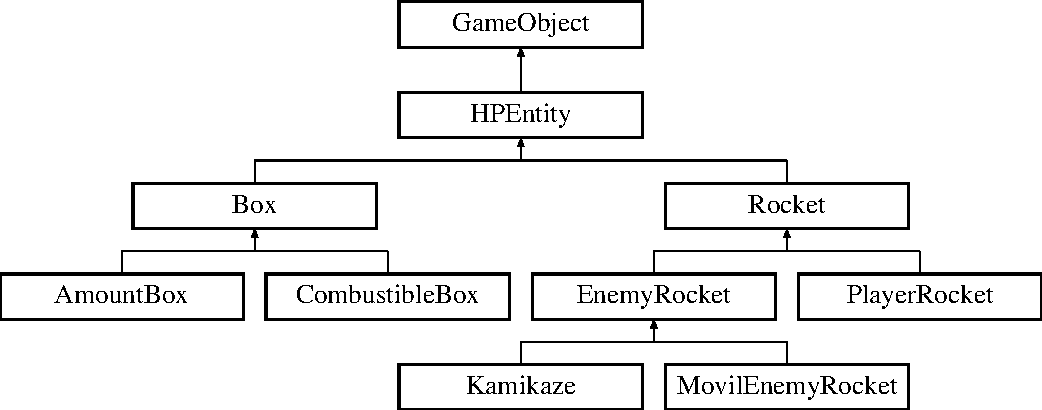
\includegraphics[height=5.000000cm]{class_h_p_entity}
\end{center}
\end{figure}
\subsection*{Public Member Functions}
\begin{DoxyCompactItemize}
\item 
\hyperlink{class_h_p_entity_a3351ec6d47cbf4e5c178b54e056adcbe}{H\-P\-Entity} (Q\-Rect p\-Rectangle, int p\-Max\-Hp)
\item 
bool \hyperlink{class_h_p_entity_a43761d5af8e1883911c3e3b7ad9170df}{is\-Dead} () const 
\item 
void \hyperlink{class_h_p_entity_a9cd0830a4369e036069aba8bdd37f703}{add\-Hit\-Points} (int p\-Hp=-\/1)
\item 
int \hyperlink{class_h_p_entity_ab66e8858b5562dd629052cd3770479c0}{get\-Hit\-Points} () const 
\item 
virtual \hyperlink{class_h_p_entity_a583b0e71da4f6e1446768e74f5c392dd}{$\sim$\-H\-P\-Entity} ()
\end{DoxyCompactItemize}
\subsection*{Protected Attributes}
\begin{DoxyCompactItemize}
\item 
int \hyperlink{class_h_p_entity_a3d72ffce5b3a795816229b5cfb1e221d}{\-\_\-\-Hp}
\item 
int \hyperlink{class_h_p_entity_a484307e81bbf22dbc7fdc11d0ee1c7d3}{\-\_\-\-Max\-Hp}
\end{DoxyCompactItemize}
\subsection*{Additional Inherited Members}


\subsection{Constructor \& Destructor Documentation}
\hypertarget{class_h_p_entity_a3351ec6d47cbf4e5c178b54e056adcbe}{\index{H\-P\-Entity@{H\-P\-Entity}!H\-P\-Entity@{H\-P\-Entity}}
\index{H\-P\-Entity@{H\-P\-Entity}!HPEntity@{H\-P\-Entity}}
\subsubsection[{H\-P\-Entity}]{\setlength{\rightskip}{0pt plus 5cm}H\-P\-Entity\-::\-H\-P\-Entity (
\begin{DoxyParamCaption}
\item[{Q\-Rect}]{p\-Rectangle, }
\item[{int}]{p\-Max\-Hp}
\end{DoxyParamCaption}
)}}\label{class_h_p_entity_a3351ec6d47cbf4e5c178b54e056adcbe}
\hypertarget{class_h_p_entity_a583b0e71da4f6e1446768e74f5c392dd}{\index{H\-P\-Entity@{H\-P\-Entity}!$\sim$\-H\-P\-Entity@{$\sim$\-H\-P\-Entity}}
\index{$\sim$\-H\-P\-Entity@{$\sim$\-H\-P\-Entity}!HPEntity@{H\-P\-Entity}}
\subsubsection[{$\sim$\-H\-P\-Entity}]{\setlength{\rightskip}{0pt plus 5cm}H\-P\-Entity\-::$\sim$\-H\-P\-Entity (
\begin{DoxyParamCaption}
{}
\end{DoxyParamCaption}
)\hspace{0.3cm}{\ttfamily [virtual]}}}\label{class_h_p_entity_a583b0e71da4f6e1446768e74f5c392dd}


\subsection{Member Function Documentation}
\hypertarget{class_h_p_entity_a9cd0830a4369e036069aba8bdd37f703}{\index{H\-P\-Entity@{H\-P\-Entity}!add\-Hit\-Points@{add\-Hit\-Points}}
\index{add\-Hit\-Points@{add\-Hit\-Points}!HPEntity@{H\-P\-Entity}}
\subsubsection[{add\-Hit\-Points}]{\setlength{\rightskip}{0pt plus 5cm}void H\-P\-Entity\-::add\-Hit\-Points (
\begin{DoxyParamCaption}
\item[{int}]{p\-Hp = {\ttfamily -\/1}}
\end{DoxyParamCaption}
)}}\label{class_h_p_entity_a9cd0830a4369e036069aba8bdd37f703}
\hypertarget{class_h_p_entity_ab66e8858b5562dd629052cd3770479c0}{\index{H\-P\-Entity@{H\-P\-Entity}!get\-Hit\-Points@{get\-Hit\-Points}}
\index{get\-Hit\-Points@{get\-Hit\-Points}!HPEntity@{H\-P\-Entity}}
\subsubsection[{get\-Hit\-Points}]{\setlength{\rightskip}{0pt plus 5cm}int H\-P\-Entity\-::get\-Hit\-Points (
\begin{DoxyParamCaption}
{}
\end{DoxyParamCaption}
) const}}\label{class_h_p_entity_ab66e8858b5562dd629052cd3770479c0}
\hypertarget{class_h_p_entity_a43761d5af8e1883911c3e3b7ad9170df}{\index{H\-P\-Entity@{H\-P\-Entity}!is\-Dead@{is\-Dead}}
\index{is\-Dead@{is\-Dead}!HPEntity@{H\-P\-Entity}}
\subsubsection[{is\-Dead}]{\setlength{\rightskip}{0pt plus 5cm}bool H\-P\-Entity\-::is\-Dead (
\begin{DoxyParamCaption}
{}
\end{DoxyParamCaption}
) const}}\label{class_h_p_entity_a43761d5af8e1883911c3e3b7ad9170df}


\subsection{Member Data Documentation}
\hypertarget{class_h_p_entity_a3d72ffce5b3a795816229b5cfb1e221d}{\index{H\-P\-Entity@{H\-P\-Entity}!\-\_\-\-Hp@{\-\_\-\-Hp}}
\index{\-\_\-\-Hp@{\-\_\-\-Hp}!HPEntity@{H\-P\-Entity}}
\subsubsection[{\-\_\-\-Hp}]{\setlength{\rightskip}{0pt plus 5cm}int H\-P\-Entity\-::\-\_\-\-Hp\hspace{0.3cm}{\ttfamily [protected]}}}\label{class_h_p_entity_a3d72ffce5b3a795816229b5cfb1e221d}
\hypertarget{class_h_p_entity_a484307e81bbf22dbc7fdc11d0ee1c7d3}{\index{H\-P\-Entity@{H\-P\-Entity}!\-\_\-\-Max\-Hp@{\-\_\-\-Max\-Hp}}
\index{\-\_\-\-Max\-Hp@{\-\_\-\-Max\-Hp}!HPEntity@{H\-P\-Entity}}
\subsubsection[{\-\_\-\-Max\-Hp}]{\setlength{\rightskip}{0pt plus 5cm}int H\-P\-Entity\-::\-\_\-\-Max\-Hp\hspace{0.3cm}{\ttfamily [protected]}}}\label{class_h_p_entity_a484307e81bbf22dbc7fdc11d0ee1c7d3}


The documentation for this class was generated from the following files\-:\begin{DoxyCompactItemize}
\item 
logic/mapobjects/\hyperlink{hpentity_8h}{hpentity.\-h}\item 
logic/mapobjects/\hyperlink{hpentity_8cpp}{hpentity.\-cpp}\end{DoxyCompactItemize}

\hypertarget{class_i_iterator}{\section{I\-Iterator$<$ E $>$ Class Template Reference}
\label{class_i_iterator}\index{I\-Iterator$<$ E $>$@{I\-Iterator$<$ E $>$}}
}


Es una interfaz para los iteradores hijos de este.  




{\ttfamily \#include $<$I\-Iterator.\-h$>$}

Inheritance diagram for I\-Iterator$<$ E $>$\-:\begin{figure}[H]
\begin{center}
\leavevmode
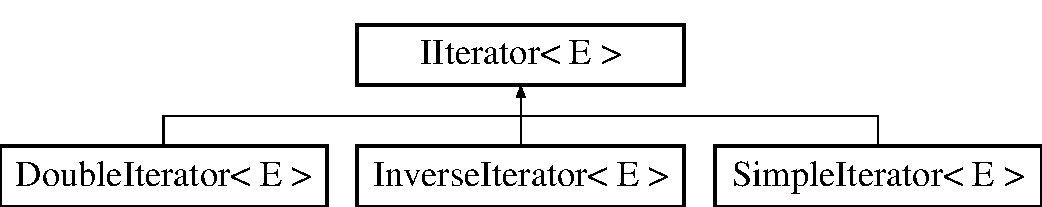
\includegraphics[height=2.000000cm]{class_i_iterator}
\end{center}
\end{figure}
\subsection*{Public Member Functions}
\begin{DoxyCompactItemize}
\item 
virtual E \hyperlink{class_i_iterator_ab1b13434e4fac20c74262dee51d1e870}{get\-Next} ()=0
\begin{DoxyCompactList}\small\item\em Obtiene el dato actual y actualiza al nodo siguiente. \end{DoxyCompactList}\item 
virtual E \hyperlink{class_i_iterator_a50f55ce1381378aad2c93f16c9b60822}{get\-Current} () const =0
\begin{DoxyCompactList}\small\item\em Obtiene el dato actual. \end{DoxyCompactList}\item 
virtual bool \hyperlink{class_i_iterator_a8a73f0fb41a66fe98e5e636378759196}{has\-Next} () const =0
\begin{DoxyCompactList}\small\item\em Verifica si tiene siguiente. \end{DoxyCompactList}\item 
\hypertarget{class_i_iterator_a46e00fa31d4f8d29232f4b1dfc27026b}{virtual \hyperlink{class_i_iterator_a46e00fa31d4f8d29232f4b1dfc27026b}{$\sim$\-I\-Iterator} ()}\label{class_i_iterator_a46e00fa31d4f8d29232f4b1dfc27026b}

\begin{DoxyCompactList}\small\item\em Liberador de memoria. \end{DoxyCompactList}\end{DoxyCompactItemize}


\subsection{Detailed Description}
\subsubsection*{template$<$class E$>$class I\-Iterator$<$ E $>$}

Es una interfaz para los iteradores hijos de este. 

\subsection{Member Function Documentation}
\hypertarget{class_i_iterator_a50f55ce1381378aad2c93f16c9b60822}{\index{I\-Iterator@{I\-Iterator}!get\-Current@{get\-Current}}
\index{get\-Current@{get\-Current}!IIterator@{I\-Iterator}}
\subsubsection[{get\-Current}]{\setlength{\rightskip}{0pt plus 5cm}template$<$class E$>$ virtual E {\bf I\-Iterator}$<$ E $>$\-::get\-Current (
\begin{DoxyParamCaption}
{}
\end{DoxyParamCaption}
) const\hspace{0.3cm}{\ttfamily [pure virtual]}}}\label{class_i_iterator_a50f55ce1381378aad2c93f16c9b60822}


Obtiene el dato actual. 

\begin{DoxyReturn}{Returns}
E el dato actual 
\end{DoxyReturn}

\begin{DoxyExceptions}{Exceptions}
{\em donthavenext} & si el dato actual es nulo \\
\hline
\end{DoxyExceptions}


Implemented in \hyperlink{class_inverse_iterator_afdbb5c310621c773da10dfb5bc3b1a4c}{Inverse\-Iterator$<$ E $>$}, \hyperlink{class_simple_iterator_ac9460c98985a20f781f351c85b8a3ba2}{Simple\-Iterator$<$ E $>$}, and \hyperlink{class_double_iterator_a756bb08f5352e270e08b72339c32e2be}{Double\-Iterator$<$ E $>$}.

\hypertarget{class_i_iterator_ab1b13434e4fac20c74262dee51d1e870}{\index{I\-Iterator@{I\-Iterator}!get\-Next@{get\-Next}}
\index{get\-Next@{get\-Next}!IIterator@{I\-Iterator}}
\subsubsection[{get\-Next}]{\setlength{\rightskip}{0pt plus 5cm}template$<$class E$>$ virtual E {\bf I\-Iterator}$<$ E $>$\-::get\-Next (
\begin{DoxyParamCaption}
{}
\end{DoxyParamCaption}
)\hspace{0.3cm}{\ttfamily [pure virtual]}}}\label{class_i_iterator_ab1b13434e4fac20c74262dee51d1e870}


Obtiene el dato actual y actualiza al nodo siguiente. 

\begin{DoxyReturn}{Returns}
E el dato actual 
\end{DoxyReturn}

\begin{DoxyExceptions}{Exceptions}
{\em donthavenext} & si el dato actual es nulo \\
\hline
\end{DoxyExceptions}


Implemented in \hyperlink{class_simple_iterator_ab01032dba9ff4f1a1c47af3082b717d5}{Simple\-Iterator$<$ E $>$}, \hyperlink{class_double_iterator_aaaa1b361a61339bfee3bf86f3f67b198}{Double\-Iterator$<$ E $>$}, and \hyperlink{class_inverse_iterator_a4c1d8ceb8264f7f8186b6244a0a62940}{Inverse\-Iterator$<$ E $>$}.

\hypertarget{class_i_iterator_a8a73f0fb41a66fe98e5e636378759196}{\index{I\-Iterator@{I\-Iterator}!has\-Next@{has\-Next}}
\index{has\-Next@{has\-Next}!IIterator@{I\-Iterator}}
\subsubsection[{has\-Next}]{\setlength{\rightskip}{0pt plus 5cm}template$<$class E$>$ virtual bool {\bf I\-Iterator}$<$ E $>$\-::has\-Next (
\begin{DoxyParamCaption}
{}
\end{DoxyParamCaption}
) const\hspace{0.3cm}{\ttfamily [pure virtual]}}}\label{class_i_iterator_a8a73f0fb41a66fe98e5e636378759196}


Verifica si tiene siguiente. 

\begin{DoxyReturn}{Returns}
true si tiene siguiente, false si no lo tiene 
\end{DoxyReturn}

\begin{DoxyExceptions}{Exceptions}
{\em donthavenext} & si el dato actual es nulo \\
\hline
\end{DoxyExceptions}


Implemented in \hyperlink{class_simple_iterator_ab946b3d707e32d4d53f15af201ea2113}{Simple\-Iterator$<$ E $>$}, \hyperlink{class_double_iterator_adb5ef4c66649e0a4ce18e38cd85904ed}{Double\-Iterator$<$ E $>$}, and \hyperlink{class_inverse_iterator_a86973781dfa84df67be2843fc4545692}{Inverse\-Iterator$<$ E $>$}.



The documentation for this class was generated from the following file\-:\begin{DoxyCompactItemize}
\item 
list/I\-Iterator.\-h\end{DoxyCompactItemize}

\hypertarget{class_i_list}{\section{I\-List$<$ E $>$ Class Template Reference}
\label{class_i_list}\index{I\-List$<$ E $>$@{I\-List$<$ E $>$}}
}


Es la interfaz de las listas.  




{\ttfamily \#include $<$I\-List.\-h$>$}

Inheritance diagram for I\-List$<$ E $>$\-:\begin{figure}[H]
\begin{center}
\leavevmode
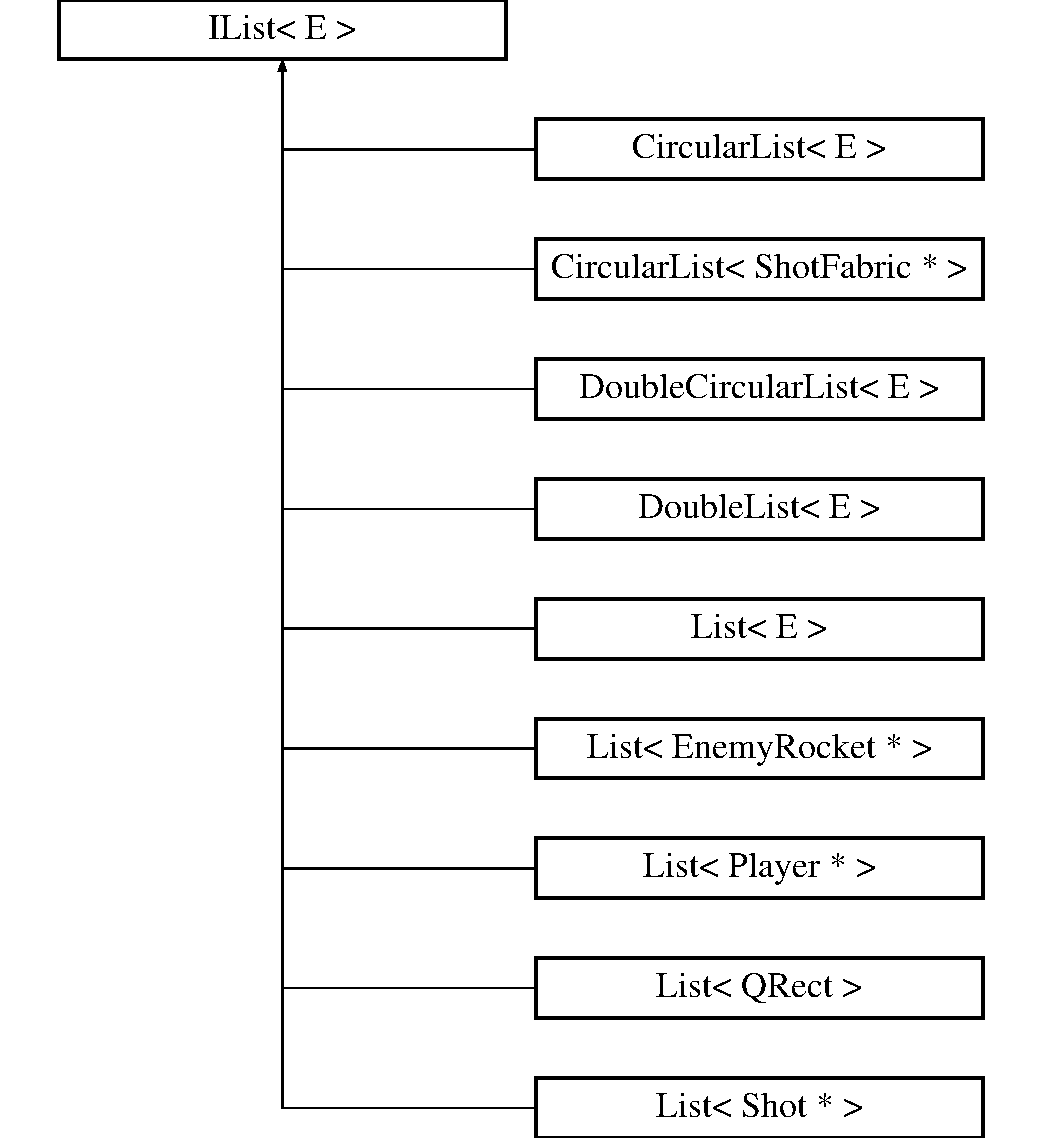
\includegraphics[height=10.000000cm]{class_i_list}
\end{center}
\end{figure}
\subsection*{Public Member Functions}
\begin{DoxyCompactItemize}
\item 
virtual void \hyperlink{class_i_list_af202dc9e748ee32238d80e57dfbcae20}{addi} (E)=0
\begin{DoxyCompactList}\small\item\em Agrega un elemento al principio de la lista. \end{DoxyCompactList}\item 
virtual void \hyperlink{class_i_list_a27500caa3d9da05aa6437d5ff56b09e2}{add} (E)=0
\begin{DoxyCompactList}\small\item\em Agregar un elemento al final de la lista. \end{DoxyCompactList}\item 
virtual bool \hyperlink{class_i_list_a70140dbc9de2b9f6e5ffd2212d5ea8b0}{add} (E, int)=0
\begin{DoxyCompactList}\small\item\em Agrega el elemento en el indice indicado. Si el indice es incorrecto no se agrega el elemento. \end{DoxyCompactList}\item 
virtual bool \hyperlink{class_i_list_a9bf7d737252dfbd4c9a5d7be36ea4231}{remove} (int)=0
\begin{DoxyCompactList}\small\item\em Remueve el dato en la posicion indicada por el parametro, en caso que el indice indicado sea incorrecto, osea que sea menor que cero o mayor o igual que el largo de la lista no alterara la lista. \end{DoxyCompactList}\item 
virtual void \hyperlink{class_i_list_a119ed658d2804aec0b9fef9325c03073}{set} (int, E)=0
\begin{DoxyCompactList}\small\item\em Setea el valor del dato que se encuentre en el indice citado con un nuevo valor. \end{DoxyCompactList}\item 
virtual E \hyperlink{class_i_list_a60570f7ee0e7474d01b2f364bad996a0}{get} (int)=0
\begin{DoxyCompactList}\small\item\em Obtiene un dato el la posicion indicada. En caso que el indice indicado sea incorrecto, osea que sea menor que cero o mayor o igual que el largo de la lista arrojara un error pues el dato esta fuera de los limites de la lista. \end{DoxyCompactList}\item 
int \hyperlink{class_i_list_a6d43df225c304c3a0abdb4c7d81274b5}{get\-Lenght} () const 
\begin{DoxyCompactList}\small\item\em Obtiene el largo de la lista. \end{DoxyCompactList}\item 
virtual \hyperlink{class_i_iterator}{I\-Iterator}$<$ E $>$ $\ast$ \hyperlink{class_i_list_a997815664cc6b20eb5dfa9968251d2cd}{get\-Iterator} ()=0
\begin{DoxyCompactList}\small\item\em Obtiene una instancia de un nuevo iterador de esta lista, y pueden obtenerse cuantas sean necesarias. pero es responsabilidad del programador eliminar mediante la palabra reservada delete. Ademas este puede ser un iterador inverso o normal, eso quiere decir que el iterador puede recorrer la lista al reves o al derecho respectivamente a los iteradores anteriormente citados. El tipo de iterador puede ser señalado con la funcion \hyperlink{class_double_circular_list_a77212c5d6ad148c99a06009a8c44128b}{Double\-Circular\-List\-::inverse\-Iteration(bool)}\end{DoxyCompactList}\item 
bool \hyperlink{class_i_list_ad21f4969c574c87a4715d45496d81d5c}{is\-Empty} () const 
\begin{DoxyCompactList}\small\item\em Verifica si la lista esta vacia. \end{DoxyCompactList}\item 
\hypertarget{class_i_list_a6ff12f7e891ea75a5554b70ed3fa0de8}{virtual \hyperlink{class_i_list_a6ff12f7e891ea75a5554b70ed3fa0de8}{$\sim$\-I\-List} ()}\label{class_i_list_a6ff12f7e891ea75a5554b70ed3fa0de8}

\begin{DoxyCompactList}\small\item\em Liberador de memoria. \end{DoxyCompactList}\end{DoxyCompactItemize}
\subsection*{Protected Attributes}
\begin{DoxyCompactItemize}
\item 
int \hyperlink{class_i_list_a64ce981ba1104bbb482068983cb5a3bc}{lenght}
\end{DoxyCompactItemize}


\subsection{Detailed Description}
\subsubsection*{template$<$class E$>$class I\-List$<$ E $>$}

Es la interfaz de las listas. 

\subsection{Member Function Documentation}
\hypertarget{class_i_list_a27500caa3d9da05aa6437d5ff56b09e2}{\index{I\-List@{I\-List}!add@{add}}
\index{add@{add}!IList@{I\-List}}
\subsubsection[{add}]{\setlength{\rightskip}{0pt plus 5cm}template$<$class E $>$ virtual void {\bf I\-List}$<$ E $>$\-::add (
\begin{DoxyParamCaption}
\item[{E}]{}
\end{DoxyParamCaption}
)\hspace{0.3cm}{\ttfamily [pure virtual]}}}\label{class_i_list_a27500caa3d9da05aa6437d5ff56b09e2}


Agregar un elemento al final de la lista. 


\begin{DoxyParams}{Parameters}
{\em data} & el elemento a agregar \\
\hline
\end{DoxyParams}


Implemented in \hyperlink{class_double_circular_list_a7691d38e77ea44d222c465f27e7d05b6}{Double\-Circular\-List$<$ E $>$}, \hyperlink{class_circular_list_a892b493309f36fb083fdd257388cfa36}{Circular\-List$<$ E $>$}, \hyperlink{class_double_list_adb96e6908d3d564722225b848350aa82}{Double\-List$<$ E $>$}, and \hyperlink{class_list_a2a130b7bc38cd968136f1f847e42d0cc}{List$<$ E $>$}.

\hypertarget{class_i_list_a70140dbc9de2b9f6e5ffd2212d5ea8b0}{\index{I\-List@{I\-List}!add@{add}}
\index{add@{add}!IList@{I\-List}}
\subsubsection[{add}]{\setlength{\rightskip}{0pt plus 5cm}template$<$class E $>$ virtual bool {\bf I\-List}$<$ E $>$\-::add (
\begin{DoxyParamCaption}
\item[{E}]{, }
\item[{int}]{}
\end{DoxyParamCaption}
)\hspace{0.3cm}{\ttfamily [pure virtual]}}}\label{class_i_list_a70140dbc9de2b9f6e5ffd2212d5ea8b0}


Agrega el elemento en el indice indicado. Si el indice es incorrecto no se agrega el elemento. 


\begin{DoxyParams}{Parameters}
{\em data} & el elemento a agregar \\
\hline
{\em index} & el indice que indica el lugar donde se agragegara \\
\hline
\end{DoxyParams}
\begin{DoxyReturn}{Returns}
si el elemento se agrega retorna true, en caso contrario retorna false 
\end{DoxyReturn}


Implemented in \hyperlink{class_double_circular_list_a6d76f7045dd9997f55c6c2feb80678da}{Double\-Circular\-List$<$ E $>$}, \hyperlink{class_circular_list_af184d3ac2e3bba683a44a6cc19392b12}{Circular\-List$<$ E $>$}, \hyperlink{class_double_list_a84e3bb8be7d67b43dd3b63d5a47f80ed}{Double\-List$<$ E $>$}, and \hyperlink{class_list_a530267346ebec244900c162de6f467e1}{List$<$ E $>$}.

\hypertarget{class_i_list_af202dc9e748ee32238d80e57dfbcae20}{\index{I\-List@{I\-List}!addi@{addi}}
\index{addi@{addi}!IList@{I\-List}}
\subsubsection[{addi}]{\setlength{\rightskip}{0pt plus 5cm}template$<$class E $>$ virtual void {\bf I\-List}$<$ E $>$\-::addi (
\begin{DoxyParamCaption}
\item[{E}]{}
\end{DoxyParamCaption}
)\hspace{0.3cm}{\ttfamily [pure virtual]}}}\label{class_i_list_af202dc9e748ee32238d80e57dfbcae20}


Agrega un elemento al principio de la lista. 


\begin{DoxyParams}{Parameters}
{\em data} & el elemento a agregar \\
\hline
\end{DoxyParams}


Implemented in \hyperlink{class_double_circular_list_ade2ef68a86a8deef4cb43d38e031906b}{Double\-Circular\-List$<$ E $>$}, \hyperlink{class_circular_list_a275c75e142e791de9a1a00691af56a73}{Circular\-List$<$ E $>$}, \hyperlink{class_double_list_a621684e61b8d9d41cd107174d9877b1e}{Double\-List$<$ E $>$}, \hyperlink{class_list_a4f0fb366c1153a4fd01826e9e6de5afc}{List$<$ E $>$}, \hyperlink{class_circular_list_a6f405f4be7946286a958e0b83937b3e2}{Circular\-List$<$ E $>$}, \hyperlink{class_double_circular_list_aee387acc4f53773302be4aa98bc779dc}{Double\-Circular\-List$<$ E $>$}, \hyperlink{class_double_list_a01623cc4b04d94c655de62ae373963b2}{Double\-List$<$ E $>$}, and \hyperlink{class_list_a92ad933f8d3a033b84a517fb6cc4111a}{List$<$ E $>$}.

\hypertarget{class_i_list_a60570f7ee0e7474d01b2f364bad996a0}{\index{I\-List@{I\-List}!get@{get}}
\index{get@{get}!IList@{I\-List}}
\subsubsection[{get}]{\setlength{\rightskip}{0pt plus 5cm}template$<$class E $>$ virtual E {\bf I\-List}$<$ E $>$\-::get (
\begin{DoxyParamCaption}
\item[{int}]{}
\end{DoxyParamCaption}
)\hspace{0.3cm}{\ttfamily [pure virtual]}}}\label{class_i_list_a60570f7ee0e7474d01b2f364bad996a0}


Obtiene un dato el la posicion indicada. En caso que el indice indicado sea incorrecto, osea que sea menor que cero o mayor o igual que el largo de la lista arrojara un error pues el dato esta fuera de los limites de la lista. 


\begin{DoxyParams}{Parameters}
{\em index} & el indice indicado \\
\hline
\end{DoxyParams}
\begin{DoxyReturn}{Returns}
data el dato buscado por el indice indicado 
\end{DoxyReturn}

\begin{DoxyExceptions}{Exceptions}
{\em indexoutbounds} & fuera de rango si index es menor que cero o index es mayor o igual que el largo de la lista \\
\hline
\end{DoxyExceptions}


Implemented in \hyperlink{class_double_circular_list_aa00bc8fd524af1ba208f85d8816dec52}{Double\-Circular\-List$<$ E $>$}, \hyperlink{class_double_list_a230a8c9c574abe9c72f8daae35127d9c}{Double\-List$<$ E $>$}, \hyperlink{class_circular_list_ad6783339c7ff05841fc62f74f809644d}{Circular\-List$<$ E $>$}, \hyperlink{class_circular_list_ad6783339c7ff05841fc62f74f809644d}{Circular\-List$<$ Shot\-Fabric $\ast$ $>$}, \hyperlink{class_list_ab081a52d7a62aa6c5550ff9762f9427f}{List$<$ E $>$}, \hyperlink{class_list_ab081a52d7a62aa6c5550ff9762f9427f}{List$<$ Player $\ast$ $>$}, \hyperlink{class_list_ab081a52d7a62aa6c5550ff9762f9427f}{List$<$ Shot $\ast$ $>$}, \hyperlink{class_list_ab081a52d7a62aa6c5550ff9762f9427f}{List$<$ Q\-Rect $>$}, and \hyperlink{class_list_ab081a52d7a62aa6c5550ff9762f9427f}{List$<$ Enemy\-Rocket $\ast$ $>$}.

\hypertarget{class_i_list_a997815664cc6b20eb5dfa9968251d2cd}{\index{I\-List@{I\-List}!get\-Iterator@{get\-Iterator}}
\index{get\-Iterator@{get\-Iterator}!IList@{I\-List}}
\subsubsection[{get\-Iterator}]{\setlength{\rightskip}{0pt plus 5cm}template$<$class E $>$ virtual {\bf I\-Iterator}$<$E$>$$\ast$ {\bf I\-List}$<$ E $>$\-::get\-Iterator (
\begin{DoxyParamCaption}
{}
\end{DoxyParamCaption}
)\hspace{0.3cm}{\ttfamily [pure virtual]}}}\label{class_i_list_a997815664cc6b20eb5dfa9968251d2cd}


Obtiene una instancia de un nuevo iterador de esta lista, y pueden obtenerse cuantas sean necesarias. pero es responsabilidad del programador eliminar mediante la palabra reservada delete. Ademas este puede ser un iterador inverso o normal, eso quiere decir que el iterador puede recorrer la lista al reves o al derecho respectivamente a los iteradores anteriormente citados. El tipo de iterador puede ser señalado con la funcion \hyperlink{class_double_circular_list_a77212c5d6ad148c99a06009a8c44128b}{Double\-Circular\-List\-::inverse\-Iteration(bool)}

\begin{DoxyReturn}{Returns}
I\-Iterator$<$\-E$>$ un puntero del iterador indicado 
\end{DoxyReturn}


Implemented in \hyperlink{class_double_circular_list_abba1430e956c7660a88f786bfd8d87ad}{Double\-Circular\-List$<$ E $>$}, \hyperlink{class_double_list_aa14e383a97e054016a6c5178165b20df}{Double\-List$<$ E $>$}, \hyperlink{class_circular_list_a43e6cf1632001b3f409c6ce531529c6e}{Circular\-List$<$ E $>$}, \hyperlink{class_circular_list_a43e6cf1632001b3f409c6ce531529c6e}{Circular\-List$<$ Shot\-Fabric $\ast$ $>$}, \hyperlink{class_list_accb5fe71cb60ba7bf0ccab362b1f87cb}{List$<$ E $>$}, \hyperlink{class_list_accb5fe71cb60ba7bf0ccab362b1f87cb}{List$<$ Player $\ast$ $>$}, \hyperlink{class_list_accb5fe71cb60ba7bf0ccab362b1f87cb}{List$<$ Shot $\ast$ $>$}, \hyperlink{class_list_accb5fe71cb60ba7bf0ccab362b1f87cb}{List$<$ Q\-Rect $>$}, and \hyperlink{class_list_accb5fe71cb60ba7bf0ccab362b1f87cb}{List$<$ Enemy\-Rocket $\ast$ $>$}.

\hypertarget{class_i_list_a6d43df225c304c3a0abdb4c7d81274b5}{\index{I\-List@{I\-List}!get\-Lenght@{get\-Lenght}}
\index{get\-Lenght@{get\-Lenght}!IList@{I\-List}}
\subsubsection[{get\-Lenght}]{\setlength{\rightskip}{0pt plus 5cm}template$<$class E $>$ int {\bf I\-List}$<$ E $>$\-::get\-Lenght (
\begin{DoxyParamCaption}
{}
\end{DoxyParamCaption}
) const}}\label{class_i_list_a6d43df225c304c3a0abdb4c7d81274b5}


Obtiene el largo de la lista. 

\begin{DoxyReturn}{Returns}
lenght el largo de la lista 
\end{DoxyReturn}
\hypertarget{class_i_list_ad21f4969c574c87a4715d45496d81d5c}{\index{I\-List@{I\-List}!is\-Empty@{is\-Empty}}
\index{is\-Empty@{is\-Empty}!IList@{I\-List}}
\subsubsection[{is\-Empty}]{\setlength{\rightskip}{0pt plus 5cm}template$<$class E $>$ bool {\bf I\-List}$<$ E $>$\-::is\-Empty (
\begin{DoxyParamCaption}
{}
\end{DoxyParamCaption}
) const}}\label{class_i_list_ad21f4969c574c87a4715d45496d81d5c}


Verifica si la lista esta vacia. 

\begin{DoxyReturn}{Returns}
true si la lista esta vacia 
\end{DoxyReturn}
\hypertarget{class_i_list_a9bf7d737252dfbd4c9a5d7be36ea4231}{\index{I\-List@{I\-List}!remove@{remove}}
\index{remove@{remove}!IList@{I\-List}}
\subsubsection[{remove}]{\setlength{\rightskip}{0pt plus 5cm}template$<$class E $>$ virtual bool {\bf I\-List}$<$ E $>$\-::remove (
\begin{DoxyParamCaption}
\item[{int}]{}
\end{DoxyParamCaption}
)\hspace{0.3cm}{\ttfamily [pure virtual]}}}\label{class_i_list_a9bf7d737252dfbd4c9a5d7be36ea4231}


Remueve el dato en la posicion indicada por el parametro, en caso que el indice indicado sea incorrecto, osea que sea menor que cero o mayor o igual que el largo de la lista no alterara la lista. 


\begin{DoxyParams}{Parameters}
{\em index} & la posicion indicada del objeto a borrar \\
\hline
\end{DoxyParams}
\begin{DoxyReturn}{Returns}
true si borra algo, false si el indice indicado es incorrecto 
\end{DoxyReturn}


Implemented in \hyperlink{class_double_circular_list_ae7ed8b6714720cb7daafa639f232ecc3}{Double\-Circular\-List$<$ E $>$}, \hyperlink{class_circular_list_a4a6acfd818a0ae9055957ec80258c60a}{Circular\-List$<$ E $>$}, \hyperlink{class_double_list_a844c2c4c3b8260bd58ab94307359fb62}{Double\-List$<$ E $>$}, \hyperlink{class_circular_list_a4a6acfd818a0ae9055957ec80258c60a}{Circular\-List$<$ Shot\-Fabric $\ast$ $>$}, \hyperlink{class_list_a46cec78299d3e23469276adf46adf9c1}{List$<$ E $>$}, \hyperlink{class_list_a46cec78299d3e23469276adf46adf9c1}{List$<$ Player $\ast$ $>$}, \hyperlink{class_list_a46cec78299d3e23469276adf46adf9c1}{List$<$ Shot $\ast$ $>$}, \hyperlink{class_list_a46cec78299d3e23469276adf46adf9c1}{List$<$ Q\-Rect $>$}, and \hyperlink{class_list_a46cec78299d3e23469276adf46adf9c1}{List$<$ Enemy\-Rocket $\ast$ $>$}.

\hypertarget{class_i_list_a119ed658d2804aec0b9fef9325c03073}{\index{I\-List@{I\-List}!set@{set}}
\index{set@{set}!IList@{I\-List}}
\subsubsection[{set}]{\setlength{\rightskip}{0pt plus 5cm}template$<$class E $>$ virtual void {\bf I\-List}$<$ E $>$\-::set (
\begin{DoxyParamCaption}
\item[{int}]{, }
\item[{E}]{}
\end{DoxyParamCaption}
)\hspace{0.3cm}{\ttfamily [pure virtual]}}}\label{class_i_list_a119ed658d2804aec0b9fef9325c03073}


Setea el valor del dato que se encuentre en el indice citado con un nuevo valor. 


\begin{DoxyParams}{Parameters}
{\em index} & el indice en el que se encuetra el dato \\
\hline
{\em data} & el dato por el que se cambiara \\
\hline
\end{DoxyParams}


Implemented in \hyperlink{class_double_circular_list_a95e0f27bda1158233015ee3ff27b3ade}{Double\-Circular\-List$<$ E $>$}, \hyperlink{class_circular_list_aa54489e11ad76bf929f92b1dce97a3a3}{Circular\-List$<$ E $>$}, \hyperlink{class_double_list_a3c95ac3c3190b347c4a343776264bf67}{Double\-List$<$ E $>$}, and \hyperlink{class_list_ac8b31be96806bd56f655436629ac2e7a}{List$<$ E $>$}.



\subsection{Member Data Documentation}
\hypertarget{class_i_list_a64ce981ba1104bbb482068983cb5a3bc}{\index{I\-List@{I\-List}!lenght@{lenght}}
\index{lenght@{lenght}!IList@{I\-List}}
\subsubsection[{lenght}]{\setlength{\rightskip}{0pt plus 5cm}template$<$class E $>$ int {\bf I\-List}$<$ E $>$\-::lenght\hspace{0.3cm}{\ttfamily [protected]}}}\label{class_i_list_a64ce981ba1104bbb482068983cb5a3bc}
T\-O\-D\-O T\-O\-D\-O 

The documentation for this class was generated from the following file\-:\begin{DoxyCompactItemize}
\item 
list/I\-List.\-h\end{DoxyCompactItemize}

\hypertarget{class_inverse_iterator}{\section{Inverse\-Iterator$<$ E $>$ Class Template Reference}
\label{class_inverse_iterator}\index{Inverse\-Iterator$<$ E $>$@{Inverse\-Iterator$<$ E $>$}}
}


Esta clase es un iterador de las listas doblemente enlazadas, ademas la actualizacion de la lista N\-O actualiza el iterador, por lo que el iterador es momentaneo. Es similar a una fotografia de una lista que no ha sido alterada si la lista se altera usando un iterador puede que el iterador falle. Por lo que es recomendable que la lista no se actualice mientras se usa un iterador. Ademas de que este iterador recorre la lista desde el dato final hasta el dato inicial.  




{\ttfamily \#include $<$Inverse\-Iterator.\-h$>$}

Inheritance diagram for Inverse\-Iterator$<$ E $>$\-:\begin{figure}[H]
\begin{center}
\leavevmode
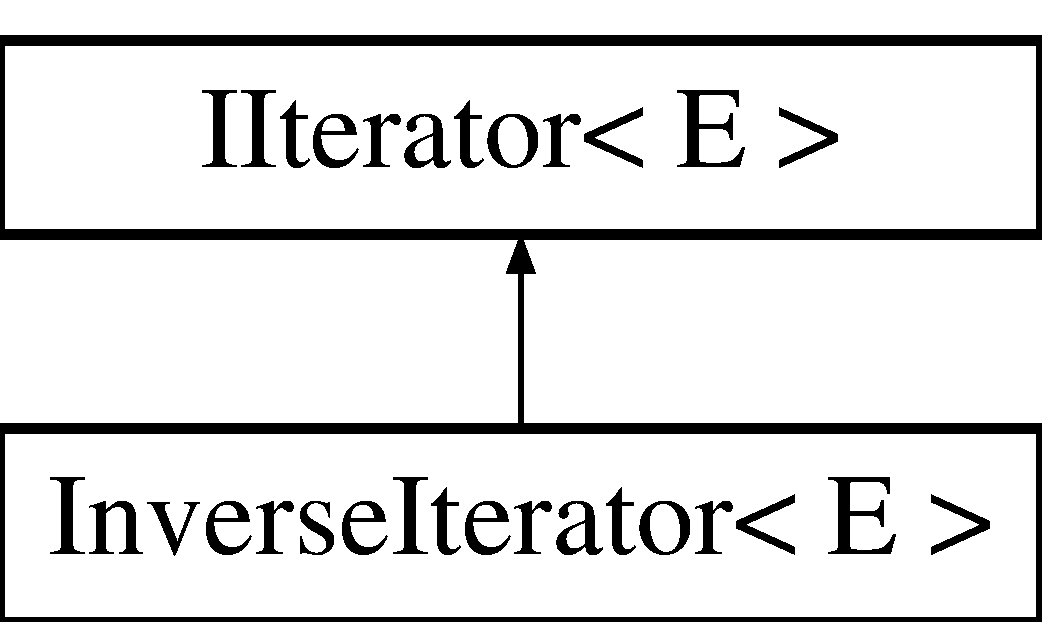
\includegraphics[height=2.000000cm]{class_inverse_iterator}
\end{center}
\end{figure}
\subsection*{Public Member Functions}
\begin{DoxyCompactItemize}
\item 
\hyperlink{class_inverse_iterator_a31703976cbdca73a1035f47509e8229d}{Inverse\-Iterator} (\hyperlink{class_double_node}{Double\-Node}$<$ E $>$ $\ast$, \hyperlink{class_double_node}{Double\-Node}$<$ E $>$ $\ast$)
\begin{DoxyCompactList}\small\item\em Metodo constructor. \end{DoxyCompactList}\item 
E \hyperlink{class_inverse_iterator_a4c1d8ceb8264f7f8186b6244a0a62940}{get\-Next} ()
\begin{DoxyCompactList}\small\item\em Obtiene el dato actual y actualiza al nodo siguiente. \end{DoxyCompactList}\item 
bool \hyperlink{class_inverse_iterator_a86973781dfa84df67be2843fc4545692}{has\-Next} () const 
\begin{DoxyCompactList}\small\item\em Obtiene el dato actual. \end{DoxyCompactList}\item 
E \hyperlink{class_inverse_iterator_afdbb5c310621c773da10dfb5bc3b1a4c}{get\-Current} () const 
\begin{DoxyCompactList}\small\item\em Verifica si tiene siguiente. \end{DoxyCompactList}\item 
virtual \hyperlink{class_inverse_iterator_ae3b6736187c1dbc82ead0277d31e5898}{$\sim$\-Inverse\-Iterator} ()
\begin{DoxyCompactList}\small\item\em liberador de memoria \end{DoxyCompactList}\end{DoxyCompactItemize}
\subsection*{Friends}
\begin{DoxyCompactItemize}
\item 
{\footnotesize template$<$class T $>$ }\\class \hyperlink{class_inverse_iterator_ad435a9844a002995926acf522128f7a8}{Double\-List}
\end{DoxyCompactItemize}


\subsection{Detailed Description}
\subsubsection*{template$<$class E$>$class Inverse\-Iterator$<$ E $>$}

Esta clase es un iterador de las listas doblemente enlazadas, ademas la actualizacion de la lista N\-O actualiza el iterador, por lo que el iterador es momentaneo. Es similar a una fotografia de una lista que no ha sido alterada si la lista se altera usando un iterador puede que el iterador falle. Por lo que es recomendable que la lista no se actualice mientras se usa un iterador. Ademas de que este iterador recorre la lista desde el dato final hasta el dato inicial. 

\subsection{Constructor \& Destructor Documentation}
\hypertarget{class_inverse_iterator_a31703976cbdca73a1035f47509e8229d}{\index{Inverse\-Iterator@{Inverse\-Iterator}!Inverse\-Iterator@{Inverse\-Iterator}}
\index{Inverse\-Iterator@{Inverse\-Iterator}!InverseIterator@{Inverse\-Iterator}}
\subsubsection[{Inverse\-Iterator}]{\setlength{\rightskip}{0pt plus 5cm}template$<$class E $>$ {\bf Inverse\-Iterator}$<$ E $>$\-::{\bf Inverse\-Iterator} (
\begin{DoxyParamCaption}
\item[{{\bf Double\-Node}$<$ E $>$ $\ast$}]{head, }
\item[{{\bf Double\-Node}$<$ E $>$ $\ast$}]{tail}
\end{DoxyParamCaption}
)}}\label{class_inverse_iterator_a31703976cbdca73a1035f47509e8229d}


Metodo constructor. 


\begin{DoxyParams}{Parameters}
{\em head} & es la cabeza el ultimo elemento de la iteracion \\
\hline
{\em tail} & es la cola por donde se iniciara la iteracion \\
\hline
\end{DoxyParams}
\hypertarget{class_inverse_iterator_ae3b6736187c1dbc82ead0277d31e5898}{\index{Inverse\-Iterator@{Inverse\-Iterator}!$\sim$\-Inverse\-Iterator@{$\sim$\-Inverse\-Iterator}}
\index{$\sim$\-Inverse\-Iterator@{$\sim$\-Inverse\-Iterator}!InverseIterator@{Inverse\-Iterator}}
\subsubsection[{$\sim$\-Inverse\-Iterator}]{\setlength{\rightskip}{0pt plus 5cm}template$<$class E$>$ virtual {\bf Inverse\-Iterator}$<$ E $>$\-::$\sim${\bf Inverse\-Iterator} (
\begin{DoxyParamCaption}
{}
\end{DoxyParamCaption}
)\hspace{0.3cm}{\ttfamily [inline]}, {\ttfamily [virtual]}}}\label{class_inverse_iterator_ae3b6736187c1dbc82ead0277d31e5898}


liberador de memoria 



\subsection{Member Function Documentation}
\hypertarget{class_inverse_iterator_afdbb5c310621c773da10dfb5bc3b1a4c}{\index{Inverse\-Iterator@{Inverse\-Iterator}!get\-Current@{get\-Current}}
\index{get\-Current@{get\-Current}!InverseIterator@{Inverse\-Iterator}}
\subsubsection[{get\-Current}]{\setlength{\rightskip}{0pt plus 5cm}template$<$class E $>$ E {\bf Inverse\-Iterator}$<$ E $>$\-::get\-Current (
\begin{DoxyParamCaption}
{}
\end{DoxyParamCaption}
) const\hspace{0.3cm}{\ttfamily [virtual]}}}\label{class_inverse_iterator_afdbb5c310621c773da10dfb5bc3b1a4c}


Verifica si tiene siguiente. 

\begin{DoxyReturn}{Returns}
true si tiene siguiente, false si no lo tiene 
\end{DoxyReturn}

\begin{DoxyExceptions}{Exceptions}
{\em donthavenext} & si el dato actual es nulo \\
\hline
\end{DoxyExceptions}


Implements \hyperlink{class_i_iterator_a50f55ce1381378aad2c93f16c9b60822}{I\-Iterator$<$ E $>$}.

\hypertarget{class_inverse_iterator_a4c1d8ceb8264f7f8186b6244a0a62940}{\index{Inverse\-Iterator@{Inverse\-Iterator}!get\-Next@{get\-Next}}
\index{get\-Next@{get\-Next}!InverseIterator@{Inverse\-Iterator}}
\subsubsection[{get\-Next}]{\setlength{\rightskip}{0pt plus 5cm}template$<$class E $>$ E {\bf Inverse\-Iterator}$<$ E $>$\-::get\-Next (
\begin{DoxyParamCaption}
{}
\end{DoxyParamCaption}
)\hspace{0.3cm}{\ttfamily [virtual]}}}\label{class_inverse_iterator_a4c1d8ceb8264f7f8186b6244a0a62940}


Obtiene el dato actual y actualiza al nodo siguiente. 

\begin{DoxyReturn}{Returns}
E el dato actual 
\end{DoxyReturn}

\begin{DoxyExceptions}{Exceptions}
{\em donthavenext} & si el dato actual es nulo \\
\hline
\end{DoxyExceptions}


Implements \hyperlink{class_i_iterator_ab1b13434e4fac20c74262dee51d1e870}{I\-Iterator$<$ E $>$}.

\hypertarget{class_inverse_iterator_a86973781dfa84df67be2843fc4545692}{\index{Inverse\-Iterator@{Inverse\-Iterator}!has\-Next@{has\-Next}}
\index{has\-Next@{has\-Next}!InverseIterator@{Inverse\-Iterator}}
\subsubsection[{has\-Next}]{\setlength{\rightskip}{0pt plus 5cm}template$<$class E $>$ bool {\bf Inverse\-Iterator}$<$ E $>$\-::has\-Next (
\begin{DoxyParamCaption}
{}
\end{DoxyParamCaption}
) const\hspace{0.3cm}{\ttfamily [virtual]}}}\label{class_inverse_iterator_a86973781dfa84df67be2843fc4545692}


Obtiene el dato actual. 

\begin{DoxyReturn}{Returns}
E el dato actual 
\end{DoxyReturn}

\begin{DoxyExceptions}{Exceptions}
{\em donthavenext} & si el dato actual es nulo \\
\hline
\end{DoxyExceptions}


Implements \hyperlink{class_i_iterator_a8a73f0fb41a66fe98e5e636378759196}{I\-Iterator$<$ E $>$}.



\subsection{Friends And Related Function Documentation}
\hypertarget{class_inverse_iterator_ad435a9844a002995926acf522128f7a8}{\index{Inverse\-Iterator@{Inverse\-Iterator}!Double\-List@{Double\-List}}
\index{Double\-List@{Double\-List}!InverseIterator@{Inverse\-Iterator}}
\subsubsection[{Double\-List}]{\setlength{\rightskip}{0pt plus 5cm}template$<$class E$>$ template$<$class T $>$ friend class {\bf Double\-List}\hspace{0.3cm}{\ttfamily [friend]}}}\label{class_inverse_iterator_ad435a9844a002995926acf522128f7a8}


The documentation for this class was generated from the following file\-:\begin{DoxyCompactItemize}
\item 
list/\hyperlink{_inverse_iterator_8h}{Inverse\-Iterator.\-h}\end{DoxyCompactItemize}

\hypertarget{class_i_ordinate_list}{\section{I\-Ordinate\-List$<$ E $>$ Class Template Reference}
\label{class_i_ordinate_list}\index{I\-Ordinate\-List$<$ E $>$@{I\-Ordinate\-List$<$ E $>$}}
}
Inheritance diagram for I\-Ordinate\-List$<$ E $>$\-:\begin{figure}[H]
\begin{center}
\leavevmode
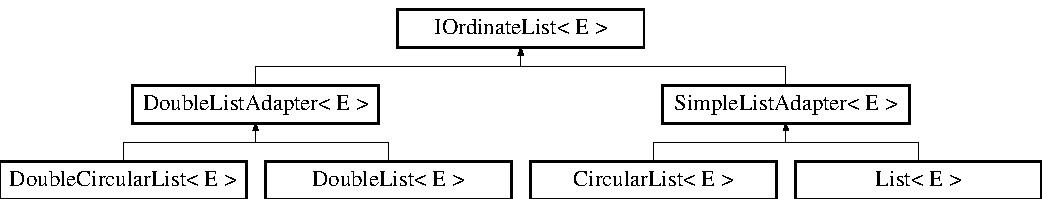
\includegraphics[height=2.675159cm]{class_i_ordinate_list}
\end{center}
\end{figure}
\subsection*{Public Member Functions}
\begin{DoxyCompactItemize}
\item 
\hypertarget{class_i_ordinate_list_af158c9cda23201b2a17e857ffcdf4cdd}{virtual bool {\bfseries add} (E p\-Data)=0}\label{class_i_ordinate_list_af158c9cda23201b2a17e857ffcdf4cdd}

\item 
\hypertarget{class_i_ordinate_list_a1015be27579a09c4805505ea3e4c4752}{virtual bool {\bfseries remove} (int p\-Index)=0}\label{class_i_ordinate_list_a1015be27579a09c4805505ea3e4c4752}

\item 
\hypertarget{class_i_ordinate_list_a596e09a9f1854ca3a570a42bd23dc816}{int {\bfseries search} (E p\-Data)}\label{class_i_ordinate_list_a596e09a9f1854ca3a570a42bd23dc816}

\item 
\hypertarget{class_i_ordinate_list_aef65b00ca705d1b106d51bff512b2021}{virtual E {\bfseries get} (int p\-Index)=0}\label{class_i_ordinate_list_aef65b00ca705d1b106d51bff512b2021}

\item 
\hypertarget{class_i_ordinate_list_a126adb3087d227a7bd47288002c6d48e}{virtual E \& {\bfseries get\-Reference} (int p\-Index)=0}\label{class_i_ordinate_list_a126adb3087d227a7bd47288002c6d48e}

\item 
\hypertarget{class_i_ordinate_list_acc0d473f2b9b464cc82b5e6cdb887b2a}{int {\bfseries get\-Lenght} ()}\label{class_i_ordinate_list_acc0d473f2b9b464cc82b5e6cdb887b2a}

\item 
\hypertarget{class_i_ordinate_list_aa555ab647394d5bf06bb4f38715bd167}{virtual \hyperlink{class_i_iterator}{I\-Iterator}$<$ E $>$ $\ast$ {\bfseries get\-Iterator} ()=0}\label{class_i_ordinate_list_aa555ab647394d5bf06bb4f38715bd167}

\end{DoxyCompactItemize}
\subsection*{Protected Attributes}
\begin{DoxyCompactItemize}
\item 
\hypertarget{class_i_ordinate_list_a28c0ecc93c212cf1fb6fa63a7227eb4a}{int {\bfseries \-\_\-lenght}}\label{class_i_ordinate_list_a28c0ecc93c212cf1fb6fa63a7227eb4a}

\end{DoxyCompactItemize}


The documentation for this class was generated from the following file\-:\begin{DoxyCompactItemize}
\item 
ordinate\-List/iordinatelist.\-h\end{DoxyCompactItemize}

\hypertarget{class_kamikaze}{\section{Kamikaze Class Reference}
\label{class_kamikaze}\index{Kamikaze@{Kamikaze}}
}


La clase kamikaze representa a una nave detectora sige al jugador y detecta su posicion.  




{\ttfamily \#include $<$kamikaze.\-h$>$}

Inheritance diagram for Kamikaze\-:\begin{figure}[H]
\begin{center}
\leavevmode
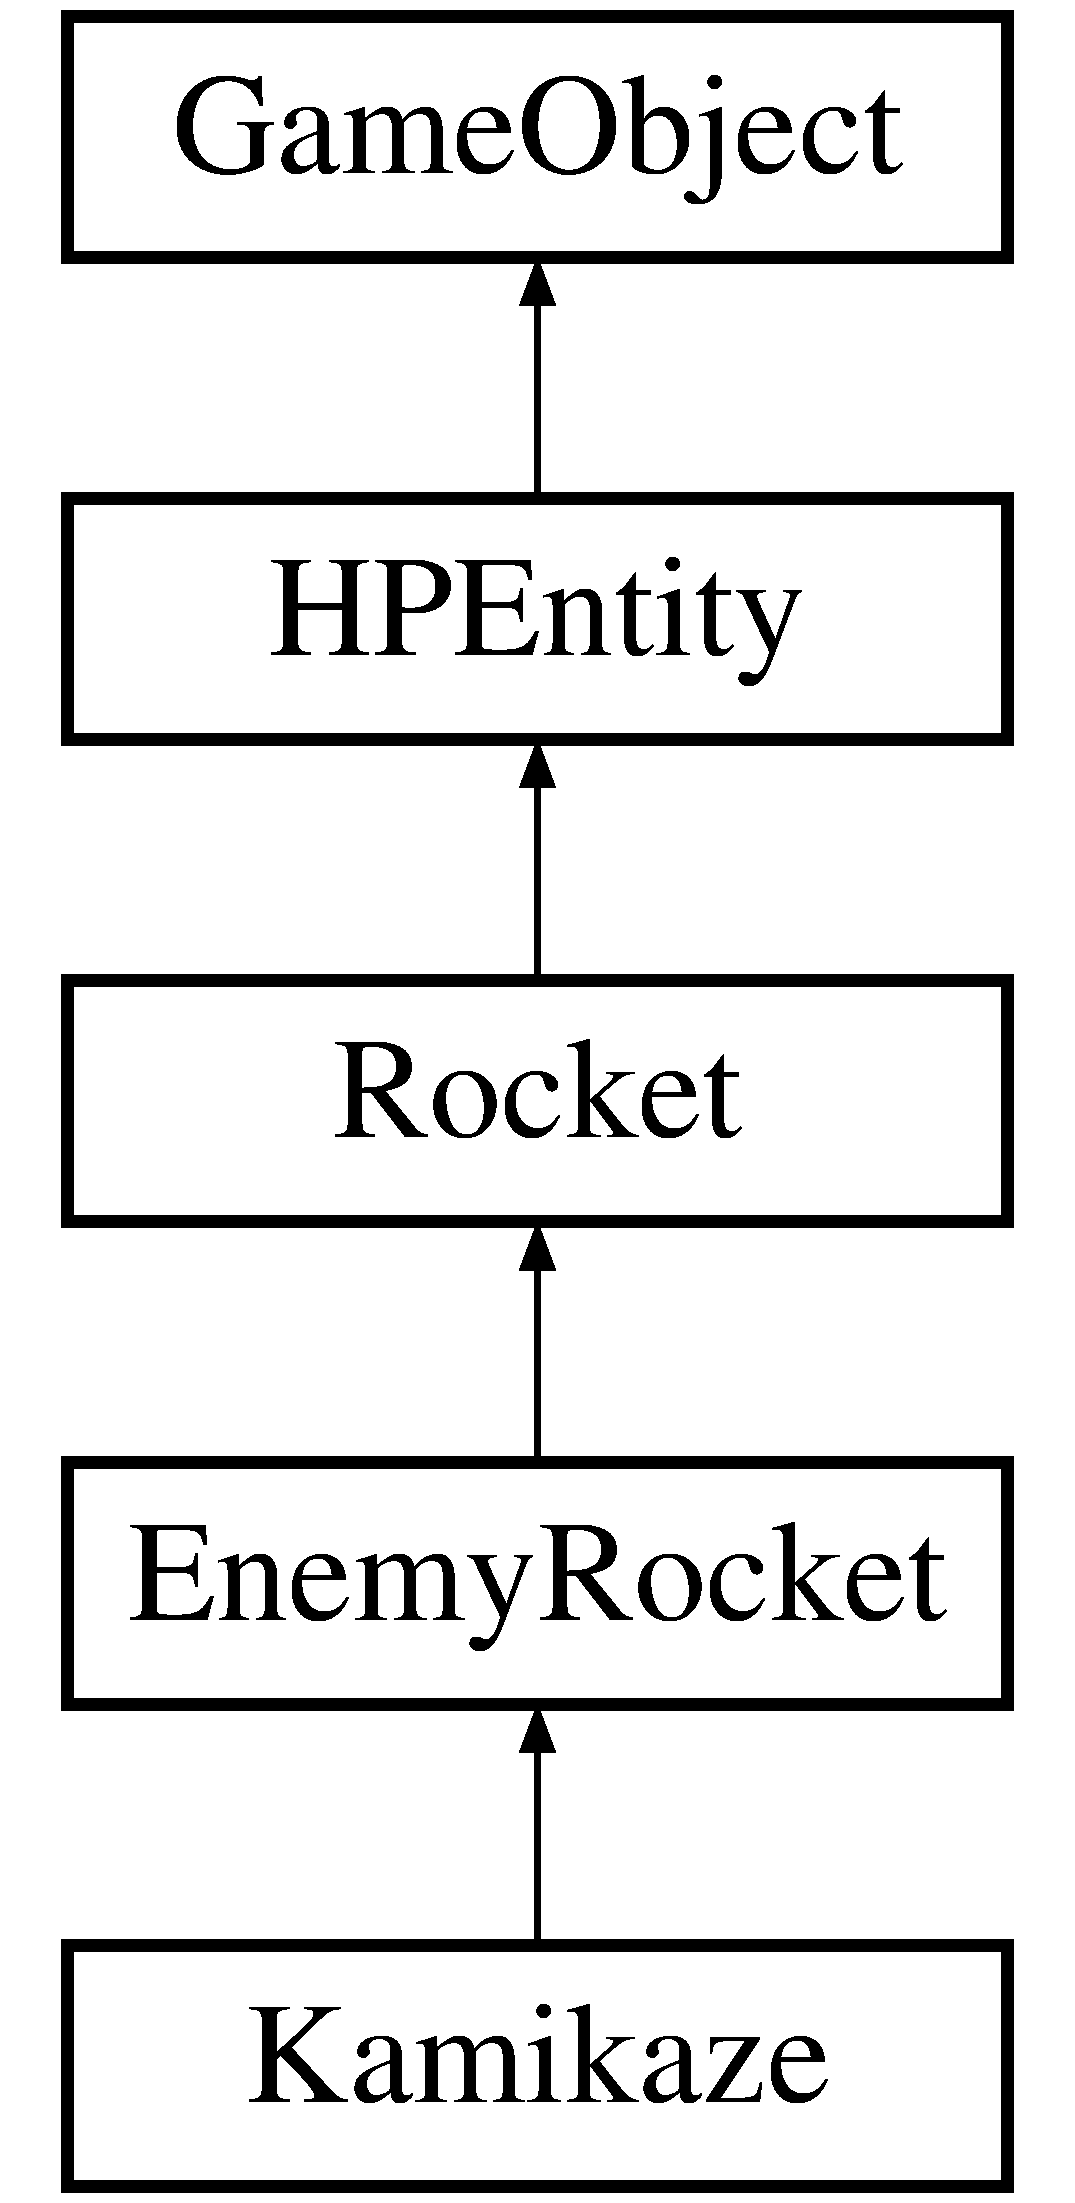
\includegraphics[height=5.000000cm]{class_kamikaze}
\end{center}
\end{figure}
\subsection*{Public Member Functions}
\begin{DoxyCompactItemize}
\item 
\hyperlink{class_kamikaze_a11b1e38216e4d3da5821b1ea31f326b0}{Kamikaze} (Q\-Rect p\-Rectangle, int p\-Max\-Hp, \hyperlink{class_player}{Player} $\ast$p\-Player\-To\-Follow)
\begin{DoxyCompactList}\small\item\em Es el metodo constructor al igual que su clase padre contiene el rectangulo que ubica la nave y tiene sus dimensiones, un entero que representa la vida maxima de este tipo de nave y finalmente incorpora un parametro nuevo un puntero al jugador que va a seguir. \end{DoxyCompactList}\item 
int \hyperlink{class_kamikaze_ae82e6a48d3e927c65fcd64269a533377}{get\-Enemy\-Type} ()
\begin{DoxyCompactList}\small\item\em Es un metodo sobrescrito y retorna la constante que representa a las naves kamizake. \end{DoxyCompactList}\item 
\hypertarget{class_kamikaze_a9af97de13e4f0306c95124f56580a8aa}{void \hyperlink{class_kamikaze_a9af97de13e4f0306c95124f56580a8aa}{update} ()}\label{class_kamikaze_a9af97de13e4f0306c95124f56580a8aa}

\begin{DoxyCompactList}\small\item\em Se sobrescribe el metodo de la clase superior y por medio de este es que se calcula la posicion de la nave kamikaze para poder seguir al jugador. \end{DoxyCompactList}\end{DoxyCompactItemize}
\subsection*{Additional Inherited Members}


\subsection{Detailed Description}
La clase kamikaze representa a una nave detectora sige al jugador y detecta su posicion. 

\subsection{Constructor \& Destructor Documentation}
\hypertarget{class_kamikaze_a11b1e38216e4d3da5821b1ea31f326b0}{\index{Kamikaze@{Kamikaze}!Kamikaze@{Kamikaze}}
\index{Kamikaze@{Kamikaze}!Kamikaze@{Kamikaze}}
\subsubsection[{Kamikaze}]{\setlength{\rightskip}{0pt plus 5cm}Kamikaze\-::\-Kamikaze (
\begin{DoxyParamCaption}
\item[{Q\-Rect}]{p\-Rectangle, }
\item[{int}]{p\-Max\-Hp, }
\item[{{\bf Player} $\ast$}]{p\-Player\-To\-Follow}
\end{DoxyParamCaption}
)}}\label{class_kamikaze_a11b1e38216e4d3da5821b1ea31f326b0}


Es el metodo constructor al igual que su clase padre contiene el rectangulo que ubica la nave y tiene sus dimensiones, un entero que representa la vida maxima de este tipo de nave y finalmente incorpora un parametro nuevo un puntero al jugador que va a seguir. 


\begin{DoxyParams}{Parameters}
{\em p\-Rectangle} & representa el tamaño y ubicacion del objeto a instanciar con el constructor \\
\hline
{\em p\-Max\-Hp} & la vida maxima de la nave kamikaze \\
\hline
{\em p\-Player\-To\-Follow} & es el puntero al jugador a seguir \\
\hline
\end{DoxyParams}


\subsection{Member Function Documentation}
\hypertarget{class_kamikaze_ae82e6a48d3e927c65fcd64269a533377}{\index{Kamikaze@{Kamikaze}!get\-Enemy\-Type@{get\-Enemy\-Type}}
\index{get\-Enemy\-Type@{get\-Enemy\-Type}!Kamikaze@{Kamikaze}}
\subsubsection[{get\-Enemy\-Type}]{\setlength{\rightskip}{0pt plus 5cm}int Kamikaze\-::get\-Enemy\-Type (
\begin{DoxyParamCaption}
{}
\end{DoxyParamCaption}
)\hspace{0.3cm}{\ttfamily [virtual]}}}\label{class_kamikaze_ae82e6a48d3e927c65fcd64269a533377}


Es un metodo sobrescrito y retorna la constante que representa a las naves kamizake. 

\begin{DoxyReturn}{Returns}
\hyperlink{class_enemy_rocket_a15caca840f5e774985fecf4295d9446d}{Enemy\-Rocket\-::\-K\-A\-M\-I\-K\-A\-Z\-E}\} 
\end{DoxyReturn}


Implements \hyperlink{class_enemy_rocket_a44e857f29c0846545743e21638391527}{Enemy\-Rocket}.



The documentation for this class was generated from the following files\-:\begin{DoxyCompactItemize}
\item 
logic/rocket/kamikaze.\-h\item 
logic/rocket/kamikaze.\-cpp\end{DoxyCompactItemize}

\hypertarget{class_kernel_game}{\section{Kernel\-Game Class Reference}
\label{class_kernel_game}\index{Kernel\-Game@{Kernel\-Game}}
}


{\ttfamily \#include $<$kernelgame.\-h$>$}

Inheritance diagram for Kernel\-Game\-:\begin{figure}[H]
\begin{center}
\leavevmode
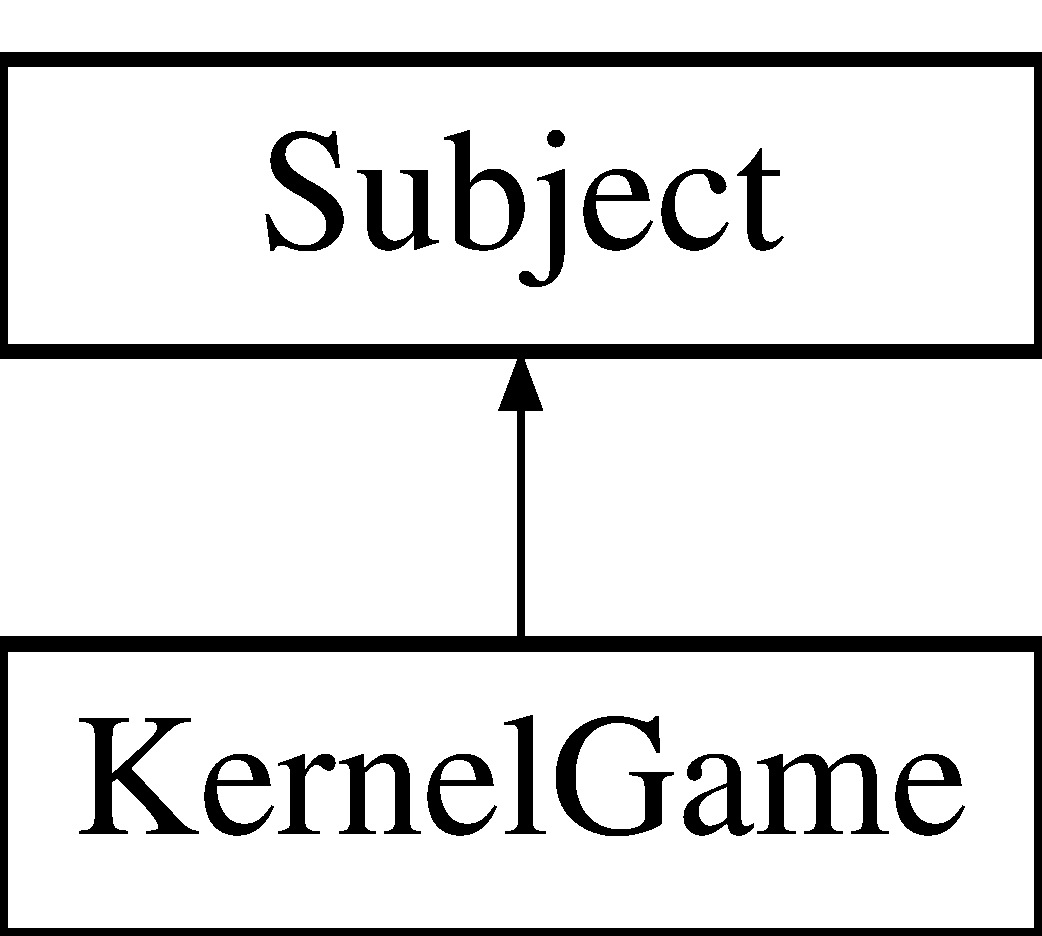
\includegraphics[height=2.000000cm]{class_kernel_game}
\end{center}
\end{figure}
\subsection*{Public Member Functions}
\begin{DoxyCompactItemize}
\item 
\hyperlink{class_kernel_game_a8d0a3d38bb42bc8ba160f83d9555f395}{Kernel\-Game} (Q\-Rect rec)
\item 
void \hyperlink{class_kernel_game_ae621056ebdaf542603f970d35843f496}{update} (Q\-Rect rec)
\item 
Q\-Rect \hyperlink{class_kernel_game_a6c6c09460150307cff306ba8edb8f56d}{get\-Player\-Rect} (int p\-Player\-Num)
\item 
Q\-Rect \hyperlink{class_kernel_game_a1867078077d9bc0bed5ea8dc783e5d4a}{get\-Rect} ()
\item 
void \hyperlink{class_kernel_game_a57642ef798e299e27b18c392fbba563f}{set\-Observer} (\hyperlink{class_observer}{Observer} $\ast$observer)
\item 
void \hyperlink{class_kernel_game_a06ed912339d619fa11c246f71e6b5ce9}{update\-Game\-Data} (int p\-Player, int v\-X, int v\-Y, bool p\-Shoot, bool p\-Pause, bool p\-Change\-Munition)
\item 
bool \hyperlink{class_kernel_game_a739246ac9cc611c114c4e1557c5da966}{is\-Running} ()
\item 
void \hyperlink{class_kernel_game_ac5ed06e95095ddb80282fb15a4c843e3}{stop} ()
\item 
void \hyperlink{class_kernel_game_ab5a6993563f54d08ac85de2675e67395}{pause\-Game} ()
\item 
bool \hyperlink{class_kernel_game_ac543f811a6f50aed646502dc35f875d2}{is\-Paused} ()
\item 
void \hyperlink{class_kernel_game_afb01399b1b5d0e8b8bbbfb84466a7d20}{notify\-All} ()
\item 
virtual \hyperlink{class_kernel_game_a7236bcaef012f43108f3dd4087c3b9fc}{$\sim$\-Kernel\-Game} ()
\end{DoxyCompactItemize}
\subsection*{Static Public Attributes}
\begin{DoxyCompactItemize}
\item 
static const int \hyperlink{class_kernel_game_a39826abf0f1c1dac2d5d7880554fc3f5}{F\-P\-S} = 24
\item 
static const int \hyperlink{class_kernel_game_a50c001388beca95ededf7b451c92325f}{P\-O\-I\-N\-T\-S\-\_\-\-P\-E\-R\-\_\-\-E\-N\-E\-M\-Y} = 50
\item 
static const int \hyperlink{class_kernel_game_a82732184131955ddcf19ed23ac8ff1ee}{S\-T\-U\-N\-\_\-\-T\-I\-M\-E} = 5
\item 
static const int \hyperlink{class_kernel_game_a675d437b5472685ab56be71d3cabad4f}{T\-I\-M\-E\-\_\-\-T\-O\-\_\-\-R\-E\-G\-E\-N\-E\-R\-A\-T\-E\-\_\-\-E\-N\-E\-M\-I\-E\-S} = \hyperlink{class_kernel_game_a39826abf0f1c1dac2d5d7880554fc3f5}{Kernel\-Game\-::\-F\-P\-S}$\ast$10
\item 
static const int \hyperlink{class_kernel_game_a6fb6f90123c4ad321e1358fd101ab166}{M\-A\-X\-\_\-\-E\-N\-E\-M\-I\-E\-S\-\_\-\-P\-E\-R\-\_\-\-C\-Y\-C\-L\-E\-S} = 9
\item 
static const int \hyperlink{class_kernel_game_a30ec2e5873f5d310826a0c56f9743997}{T\-I\-M\-E\-\_\-\-T\-O\-\_\-\-R\-E\-G\-E\-N\-E\-R\-A\-T\-E\-\_\-\-H\-P\-B\-O\-X\-E\-S} =\hyperlink{class_kernel_game_a39826abf0f1c1dac2d5d7880554fc3f5}{Kernel\-Game\-::\-F\-P\-S}$\ast$15
\item 
static const int \hyperlink{class_kernel_game_a692c5bb0576ed461c8e83261aa4f407c}{T\-I\-M\-E\-\_\-\-T\-O\-\_\-\-B\-A\-D\-\_\-\-H\-P\-B\-O\-X} = 3$\ast$\hyperlink{class_kernel_game_a39826abf0f1c1dac2d5d7880554fc3f5}{Kernel\-Game\-::\-F\-P\-S}
\item 
static const int \hyperlink{class_kernel_game_a4481548e4416ba164f867e3f1400b2ec}{A\-N\-Y\-\_\-\-B\-O\-X\-\_\-\-H\-E\-I\-G\-H\-T} = 54
\item 
static const int \hyperlink{class_kernel_game_a76023e94d4cc0df01ddda95f0d9c200d}{A\-N\-Y\-\_\-\-B\-O\-X\-\_\-\-W\-I\-D\-T\-H} = 54
\end{DoxyCompactItemize}


\subsection{Constructor \& Destructor Documentation}
\hypertarget{class_kernel_game_a8d0a3d38bb42bc8ba160f83d9555f395}{\index{Kernel\-Game@{Kernel\-Game}!Kernel\-Game@{Kernel\-Game}}
\index{Kernel\-Game@{Kernel\-Game}!KernelGame@{Kernel\-Game}}
\subsubsection[{Kernel\-Game}]{\setlength{\rightskip}{0pt plus 5cm}Kernel\-Game\-::\-Kernel\-Game (
\begin{DoxyParamCaption}
\item[{Q\-Rect}]{rec}
\end{DoxyParamCaption}
)}}\label{class_kernel_game_a8d0a3d38bb42bc8ba160f83d9555f395}
\hypertarget{class_kernel_game_a7236bcaef012f43108f3dd4087c3b9fc}{\index{Kernel\-Game@{Kernel\-Game}!$\sim$\-Kernel\-Game@{$\sim$\-Kernel\-Game}}
\index{$\sim$\-Kernel\-Game@{$\sim$\-Kernel\-Game}!KernelGame@{Kernel\-Game}}
\subsubsection[{$\sim$\-Kernel\-Game}]{\setlength{\rightskip}{0pt plus 5cm}Kernel\-Game\-::$\sim$\-Kernel\-Game (
\begin{DoxyParamCaption}
{}
\end{DoxyParamCaption}
)\hspace{0.3cm}{\ttfamily [virtual]}}}\label{class_kernel_game_a7236bcaef012f43108f3dd4087c3b9fc}


\subsection{Member Function Documentation}
\hypertarget{class_kernel_game_a6c6c09460150307cff306ba8edb8f56d}{\index{Kernel\-Game@{Kernel\-Game}!get\-Player\-Rect@{get\-Player\-Rect}}
\index{get\-Player\-Rect@{get\-Player\-Rect}!KernelGame@{Kernel\-Game}}
\subsubsection[{get\-Player\-Rect}]{\setlength{\rightskip}{0pt plus 5cm}Q\-Rect Kernel\-Game\-::get\-Player\-Rect (
\begin{DoxyParamCaption}
\item[{int}]{p\-Player\-Num}
\end{DoxyParamCaption}
)}}\label{class_kernel_game_a6c6c09460150307cff306ba8edb8f56d}
\hypertarget{class_kernel_game_a1867078077d9bc0bed5ea8dc783e5d4a}{\index{Kernel\-Game@{Kernel\-Game}!get\-Rect@{get\-Rect}}
\index{get\-Rect@{get\-Rect}!KernelGame@{Kernel\-Game}}
\subsubsection[{get\-Rect}]{\setlength{\rightskip}{0pt plus 5cm}Q\-Rect Kernel\-Game\-::get\-Rect (
\begin{DoxyParamCaption}
{}
\end{DoxyParamCaption}
)\hspace{0.3cm}{\ttfamily [inline]}}}\label{class_kernel_game_a1867078077d9bc0bed5ea8dc783e5d4a}
\hypertarget{class_kernel_game_ac543f811a6f50aed646502dc35f875d2}{\index{Kernel\-Game@{Kernel\-Game}!is\-Paused@{is\-Paused}}
\index{is\-Paused@{is\-Paused}!KernelGame@{Kernel\-Game}}
\subsubsection[{is\-Paused}]{\setlength{\rightskip}{0pt plus 5cm}bool Kernel\-Game\-::is\-Paused (
\begin{DoxyParamCaption}
{}
\end{DoxyParamCaption}
)}}\label{class_kernel_game_ac543f811a6f50aed646502dc35f875d2}
\hypertarget{class_kernel_game_a739246ac9cc611c114c4e1557c5da966}{\index{Kernel\-Game@{Kernel\-Game}!is\-Running@{is\-Running}}
\index{is\-Running@{is\-Running}!KernelGame@{Kernel\-Game}}
\subsubsection[{is\-Running}]{\setlength{\rightskip}{0pt plus 5cm}bool Kernel\-Game\-::is\-Running (
\begin{DoxyParamCaption}
{}
\end{DoxyParamCaption}
)}}\label{class_kernel_game_a739246ac9cc611c114c4e1557c5da966}
\hypertarget{class_kernel_game_afb01399b1b5d0e8b8bbbfb84466a7d20}{\index{Kernel\-Game@{Kernel\-Game}!notify\-All@{notify\-All}}
\index{notify\-All@{notify\-All}!KernelGame@{Kernel\-Game}}
\subsubsection[{notify\-All}]{\setlength{\rightskip}{0pt plus 5cm}void Kernel\-Game\-::notify\-All (
\begin{DoxyParamCaption}
{}
\end{DoxyParamCaption}
)\hspace{0.3cm}{\ttfamily [virtual]}}}\label{class_kernel_game_afb01399b1b5d0e8b8bbbfb84466a7d20}


Implements \hyperlink{class_subject_a7ef335c1bea008ee4d3dada9db2db50d}{Subject}.

\hypertarget{class_kernel_game_ab5a6993563f54d08ac85de2675e67395}{\index{Kernel\-Game@{Kernel\-Game}!pause\-Game@{pause\-Game}}
\index{pause\-Game@{pause\-Game}!KernelGame@{Kernel\-Game}}
\subsubsection[{pause\-Game}]{\setlength{\rightskip}{0pt plus 5cm}void Kernel\-Game\-::pause\-Game (
\begin{DoxyParamCaption}
{}
\end{DoxyParamCaption}
)}}\label{class_kernel_game_ab5a6993563f54d08ac85de2675e67395}
\hypertarget{class_kernel_game_a57642ef798e299e27b18c392fbba563f}{\index{Kernel\-Game@{Kernel\-Game}!set\-Observer@{set\-Observer}}
\index{set\-Observer@{set\-Observer}!KernelGame@{Kernel\-Game}}
\subsubsection[{set\-Observer}]{\setlength{\rightskip}{0pt plus 5cm}void Kernel\-Game\-::set\-Observer (
\begin{DoxyParamCaption}
\item[{{\bf Observer} $\ast$}]{observer}
\end{DoxyParamCaption}
)}}\label{class_kernel_game_a57642ef798e299e27b18c392fbba563f}
\hypertarget{class_kernel_game_ac5ed06e95095ddb80282fb15a4c843e3}{\index{Kernel\-Game@{Kernel\-Game}!stop@{stop}}
\index{stop@{stop}!KernelGame@{Kernel\-Game}}
\subsubsection[{stop}]{\setlength{\rightskip}{0pt plus 5cm}void Kernel\-Game\-::stop (
\begin{DoxyParamCaption}
{}
\end{DoxyParamCaption}
)}}\label{class_kernel_game_ac5ed06e95095ddb80282fb15a4c843e3}
\hypertarget{class_kernel_game_ae621056ebdaf542603f970d35843f496}{\index{Kernel\-Game@{Kernel\-Game}!update@{update}}
\index{update@{update}!KernelGame@{Kernel\-Game}}
\subsubsection[{update}]{\setlength{\rightskip}{0pt plus 5cm}void Kernel\-Game\-::update (
\begin{DoxyParamCaption}
\item[{Q\-Rect}]{rec}
\end{DoxyParamCaption}
)}}\label{class_kernel_game_ae621056ebdaf542603f970d35843f496}
std\-::cout $<$$<$ \char`\"{}cantidad de disparos jugador\char`\"{} $<$$<$ \-\_\-\-Players.\-get(0)-\/$>$get\-Player\-Shots()-\/$>$get\-Lenght() $<$$<$ std\-::endl; std\-::cout $<$$<$ \char`\"{}cantidad de disparos enemigos\char`\"{} $<$$<$ \-\_\-\-Enemies\-Shots.\-get\-Lenght() $<$$<$ std\-::endl; std\-::cout $<$$<$ \char`\"{}cantidad de enemigos\char`\"{} $<$$<$ \-\_\-\-Enemies.\-get\-Lenght() $<$$<$ std\-::endl;\hypertarget{class_kernel_game_a06ed912339d619fa11c246f71e6b5ce9}{\index{Kernel\-Game@{Kernel\-Game}!update\-Game\-Data@{update\-Game\-Data}}
\index{update\-Game\-Data@{update\-Game\-Data}!KernelGame@{Kernel\-Game}}
\subsubsection[{update\-Game\-Data}]{\setlength{\rightskip}{0pt plus 5cm}void Kernel\-Game\-::update\-Game\-Data (
\begin{DoxyParamCaption}
\item[{int}]{p\-Player, }
\item[{int}]{v\-X, }
\item[{int}]{v\-Y, }
\item[{bool}]{p\-Shoot, }
\item[{bool}]{p\-Pause, }
\item[{bool}]{p\-Change\-Munition}
\end{DoxyParamCaption}
)}}\label{class_kernel_game_a06ed912339d619fa11c246f71e6b5ce9}


\subsection{Member Data Documentation}
\hypertarget{class_kernel_game_a4481548e4416ba164f867e3f1400b2ec}{\index{Kernel\-Game@{Kernel\-Game}!A\-N\-Y\-\_\-\-B\-O\-X\-\_\-\-H\-E\-I\-G\-H\-T@{A\-N\-Y\-\_\-\-B\-O\-X\-\_\-\-H\-E\-I\-G\-H\-T}}
\index{A\-N\-Y\-\_\-\-B\-O\-X\-\_\-\-H\-E\-I\-G\-H\-T@{A\-N\-Y\-\_\-\-B\-O\-X\-\_\-\-H\-E\-I\-G\-H\-T}!KernelGame@{Kernel\-Game}}
\subsubsection[{A\-N\-Y\-\_\-\-B\-O\-X\-\_\-\-H\-E\-I\-G\-H\-T}]{\setlength{\rightskip}{0pt plus 5cm}const int Kernel\-Game\-::\-A\-N\-Y\-\_\-\-B\-O\-X\-\_\-\-H\-E\-I\-G\-H\-T = 54\hspace{0.3cm}{\ttfamily [static]}}}\label{class_kernel_game_a4481548e4416ba164f867e3f1400b2ec}
\hypertarget{class_kernel_game_a76023e94d4cc0df01ddda95f0d9c200d}{\index{Kernel\-Game@{Kernel\-Game}!A\-N\-Y\-\_\-\-B\-O\-X\-\_\-\-W\-I\-D\-T\-H@{A\-N\-Y\-\_\-\-B\-O\-X\-\_\-\-W\-I\-D\-T\-H}}
\index{A\-N\-Y\-\_\-\-B\-O\-X\-\_\-\-W\-I\-D\-T\-H@{A\-N\-Y\-\_\-\-B\-O\-X\-\_\-\-W\-I\-D\-T\-H}!KernelGame@{Kernel\-Game}}
\subsubsection[{A\-N\-Y\-\_\-\-B\-O\-X\-\_\-\-W\-I\-D\-T\-H}]{\setlength{\rightskip}{0pt plus 5cm}const int Kernel\-Game\-::\-A\-N\-Y\-\_\-\-B\-O\-X\-\_\-\-W\-I\-D\-T\-H = 54\hspace{0.3cm}{\ttfamily [static]}}}\label{class_kernel_game_a76023e94d4cc0df01ddda95f0d9c200d}
\hypertarget{class_kernel_game_a39826abf0f1c1dac2d5d7880554fc3f5}{\index{Kernel\-Game@{Kernel\-Game}!F\-P\-S@{F\-P\-S}}
\index{F\-P\-S@{F\-P\-S}!KernelGame@{Kernel\-Game}}
\subsubsection[{F\-P\-S}]{\setlength{\rightskip}{0pt plus 5cm}const int Kernel\-Game\-::\-F\-P\-S = 24\hspace{0.3cm}{\ttfamily [static]}}}\label{class_kernel_game_a39826abf0f1c1dac2d5d7880554fc3f5}
\hypertarget{class_kernel_game_a6fb6f90123c4ad321e1358fd101ab166}{\index{Kernel\-Game@{Kernel\-Game}!M\-A\-X\-\_\-\-E\-N\-E\-M\-I\-E\-S\-\_\-\-P\-E\-R\-\_\-\-C\-Y\-C\-L\-E\-S@{M\-A\-X\-\_\-\-E\-N\-E\-M\-I\-E\-S\-\_\-\-P\-E\-R\-\_\-\-C\-Y\-C\-L\-E\-S}}
\index{M\-A\-X\-\_\-\-E\-N\-E\-M\-I\-E\-S\-\_\-\-P\-E\-R\-\_\-\-C\-Y\-C\-L\-E\-S@{M\-A\-X\-\_\-\-E\-N\-E\-M\-I\-E\-S\-\_\-\-P\-E\-R\-\_\-\-C\-Y\-C\-L\-E\-S}!KernelGame@{Kernel\-Game}}
\subsubsection[{M\-A\-X\-\_\-\-E\-N\-E\-M\-I\-E\-S\-\_\-\-P\-E\-R\-\_\-\-C\-Y\-C\-L\-E\-S}]{\setlength{\rightskip}{0pt plus 5cm}const int Kernel\-Game\-::\-M\-A\-X\-\_\-\-E\-N\-E\-M\-I\-E\-S\-\_\-\-P\-E\-R\-\_\-\-C\-Y\-C\-L\-E\-S = 9\hspace{0.3cm}{\ttfamily [static]}}}\label{class_kernel_game_a6fb6f90123c4ad321e1358fd101ab166}
\hypertarget{class_kernel_game_a50c001388beca95ededf7b451c92325f}{\index{Kernel\-Game@{Kernel\-Game}!P\-O\-I\-N\-T\-S\-\_\-\-P\-E\-R\-\_\-\-E\-N\-E\-M\-Y@{P\-O\-I\-N\-T\-S\-\_\-\-P\-E\-R\-\_\-\-E\-N\-E\-M\-Y}}
\index{P\-O\-I\-N\-T\-S\-\_\-\-P\-E\-R\-\_\-\-E\-N\-E\-M\-Y@{P\-O\-I\-N\-T\-S\-\_\-\-P\-E\-R\-\_\-\-E\-N\-E\-M\-Y}!KernelGame@{Kernel\-Game}}
\subsubsection[{P\-O\-I\-N\-T\-S\-\_\-\-P\-E\-R\-\_\-\-E\-N\-E\-M\-Y}]{\setlength{\rightskip}{0pt plus 5cm}const int Kernel\-Game\-::\-P\-O\-I\-N\-T\-S\-\_\-\-P\-E\-R\-\_\-\-E\-N\-E\-M\-Y = 50\hspace{0.3cm}{\ttfamily [static]}}}\label{class_kernel_game_a50c001388beca95ededf7b451c92325f}
\hypertarget{class_kernel_game_a82732184131955ddcf19ed23ac8ff1ee}{\index{Kernel\-Game@{Kernel\-Game}!S\-T\-U\-N\-\_\-\-T\-I\-M\-E@{S\-T\-U\-N\-\_\-\-T\-I\-M\-E}}
\index{S\-T\-U\-N\-\_\-\-T\-I\-M\-E@{S\-T\-U\-N\-\_\-\-T\-I\-M\-E}!KernelGame@{Kernel\-Game}}
\subsubsection[{S\-T\-U\-N\-\_\-\-T\-I\-M\-E}]{\setlength{\rightskip}{0pt plus 5cm}const int Kernel\-Game\-::\-S\-T\-U\-N\-\_\-\-T\-I\-M\-E = 5\hspace{0.3cm}{\ttfamily [static]}}}\label{class_kernel_game_a82732184131955ddcf19ed23ac8ff1ee}
\hypertarget{class_kernel_game_a692c5bb0576ed461c8e83261aa4f407c}{\index{Kernel\-Game@{Kernel\-Game}!T\-I\-M\-E\-\_\-\-T\-O\-\_\-\-B\-A\-D\-\_\-\-H\-P\-B\-O\-X@{T\-I\-M\-E\-\_\-\-T\-O\-\_\-\-B\-A\-D\-\_\-\-H\-P\-B\-O\-X}}
\index{T\-I\-M\-E\-\_\-\-T\-O\-\_\-\-B\-A\-D\-\_\-\-H\-P\-B\-O\-X@{T\-I\-M\-E\-\_\-\-T\-O\-\_\-\-B\-A\-D\-\_\-\-H\-P\-B\-O\-X}!KernelGame@{Kernel\-Game}}
\subsubsection[{T\-I\-M\-E\-\_\-\-T\-O\-\_\-\-B\-A\-D\-\_\-\-H\-P\-B\-O\-X}]{\setlength{\rightskip}{0pt plus 5cm}const int Kernel\-Game\-::\-T\-I\-M\-E\-\_\-\-T\-O\-\_\-\-B\-A\-D\-\_\-\-H\-P\-B\-O\-X = 3$\ast${\bf Kernel\-Game\-::\-F\-P\-S}\hspace{0.3cm}{\ttfamily [static]}}}\label{class_kernel_game_a692c5bb0576ed461c8e83261aa4f407c}
\hypertarget{class_kernel_game_a675d437b5472685ab56be71d3cabad4f}{\index{Kernel\-Game@{Kernel\-Game}!T\-I\-M\-E\-\_\-\-T\-O\-\_\-\-R\-E\-G\-E\-N\-E\-R\-A\-T\-E\-\_\-\-E\-N\-E\-M\-I\-E\-S@{T\-I\-M\-E\-\_\-\-T\-O\-\_\-\-R\-E\-G\-E\-N\-E\-R\-A\-T\-E\-\_\-\-E\-N\-E\-M\-I\-E\-S}}
\index{T\-I\-M\-E\-\_\-\-T\-O\-\_\-\-R\-E\-G\-E\-N\-E\-R\-A\-T\-E\-\_\-\-E\-N\-E\-M\-I\-E\-S@{T\-I\-M\-E\-\_\-\-T\-O\-\_\-\-R\-E\-G\-E\-N\-E\-R\-A\-T\-E\-\_\-\-E\-N\-E\-M\-I\-E\-S}!KernelGame@{Kernel\-Game}}
\subsubsection[{T\-I\-M\-E\-\_\-\-T\-O\-\_\-\-R\-E\-G\-E\-N\-E\-R\-A\-T\-E\-\_\-\-E\-N\-E\-M\-I\-E\-S}]{\setlength{\rightskip}{0pt plus 5cm}const int Kernel\-Game\-::\-T\-I\-M\-E\-\_\-\-T\-O\-\_\-\-R\-E\-G\-E\-N\-E\-R\-A\-T\-E\-\_\-\-E\-N\-E\-M\-I\-E\-S = {\bf Kernel\-Game\-::\-F\-P\-S}$\ast$10\hspace{0.3cm}{\ttfamily [static]}}}\label{class_kernel_game_a675d437b5472685ab56be71d3cabad4f}
\hypertarget{class_kernel_game_a30ec2e5873f5d310826a0c56f9743997}{\index{Kernel\-Game@{Kernel\-Game}!T\-I\-M\-E\-\_\-\-T\-O\-\_\-\-R\-E\-G\-E\-N\-E\-R\-A\-T\-E\-\_\-\-H\-P\-B\-O\-X\-E\-S@{T\-I\-M\-E\-\_\-\-T\-O\-\_\-\-R\-E\-G\-E\-N\-E\-R\-A\-T\-E\-\_\-\-H\-P\-B\-O\-X\-E\-S}}
\index{T\-I\-M\-E\-\_\-\-T\-O\-\_\-\-R\-E\-G\-E\-N\-E\-R\-A\-T\-E\-\_\-\-H\-P\-B\-O\-X\-E\-S@{T\-I\-M\-E\-\_\-\-T\-O\-\_\-\-R\-E\-G\-E\-N\-E\-R\-A\-T\-E\-\_\-\-H\-P\-B\-O\-X\-E\-S}!KernelGame@{Kernel\-Game}}
\subsubsection[{T\-I\-M\-E\-\_\-\-T\-O\-\_\-\-R\-E\-G\-E\-N\-E\-R\-A\-T\-E\-\_\-\-H\-P\-B\-O\-X\-E\-S}]{\setlength{\rightskip}{0pt plus 5cm}const int Kernel\-Game\-::\-T\-I\-M\-E\-\_\-\-T\-O\-\_\-\-R\-E\-G\-E\-N\-E\-R\-A\-T\-E\-\_\-\-H\-P\-B\-O\-X\-E\-S ={\bf Kernel\-Game\-::\-F\-P\-S}$\ast$15\hspace{0.3cm}{\ttfamily [static]}}}\label{class_kernel_game_a30ec2e5873f5d310826a0c56f9743997}


The documentation for this class was generated from the following files\-:\begin{DoxyCompactItemize}
\item 
logic/\hyperlink{kernelgame_8h}{kernelgame.\-h}\item 
logic/\hyperlink{kernelgame_8cpp}{kernelgame.\-cpp}\end{DoxyCompactItemize}

\hypertarget{class_key_updater}{\section{Key\-Updater Class Reference}
\label{class_key_updater}\index{Key\-Updater@{Key\-Updater}}
}
Inheritance diagram for Key\-Updater\-:\begin{figure}[H]
\begin{center}
\leavevmode
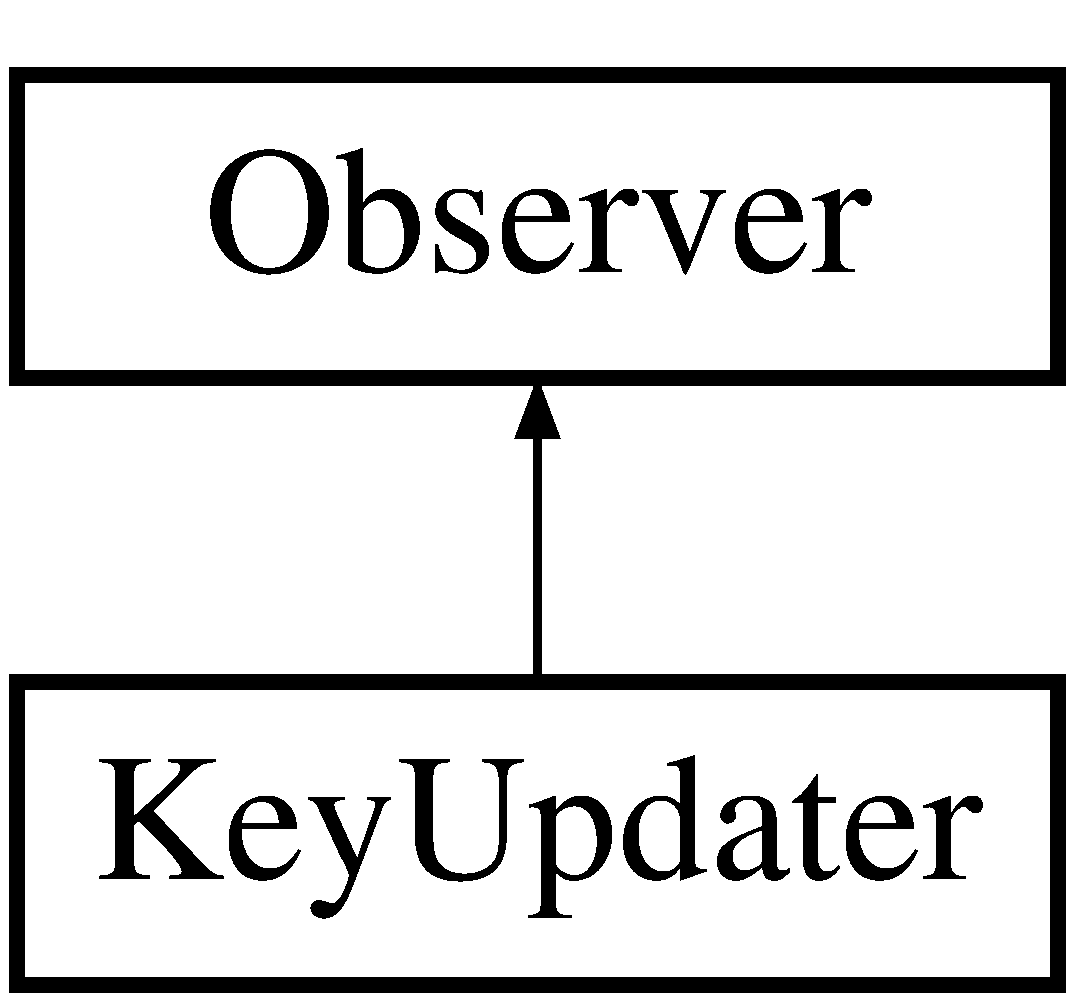
\includegraphics[height=2.000000cm]{class_key_updater}
\end{center}
\end{figure}
\subsection*{Public Member Functions}
\begin{DoxyCompactItemize}
\item 
\hypertarget{class_key_updater_a9e36344e5b6ea74cd35d64b00b108a18}{{\bfseries Key\-Updater} (Kernel\-Game $\ast$kg)}\label{class_key_updater_a9e36344e5b6ea74cd35d64b00b108a18}

\item 
\hypertarget{class_key_updater_ae98e44fb4a0be038fd6482bfae40007e}{void {\bfseries update} (google\-::protobuf\-::\-Message $\ast$p\-Message)}\label{class_key_updater_ae98e44fb4a0be038fd6482bfae40007e}

\end{DoxyCompactItemize}


The documentation for this class was generated from the following files\-:\begin{DoxyCompactItemize}
\item 
/home/cristianfernando/\-Documentos/git/\-Crazy\-River\-Ride/src/keyupdater.\-h\item 
/home/cristianfernando/\-Documentos/git/\-Crazy\-River\-Ride/src/keyupdater.\-cpp\end{DoxyCompactItemize}

\hypertarget{class_linear_shot}{\section{Linear\-Shot Class Reference}
\label{class_linear_shot}\index{Linear\-Shot@{Linear\-Shot}}
}
Inheritance diagram for Linear\-Shot\-:\begin{figure}[H]
\begin{center}
\leavevmode
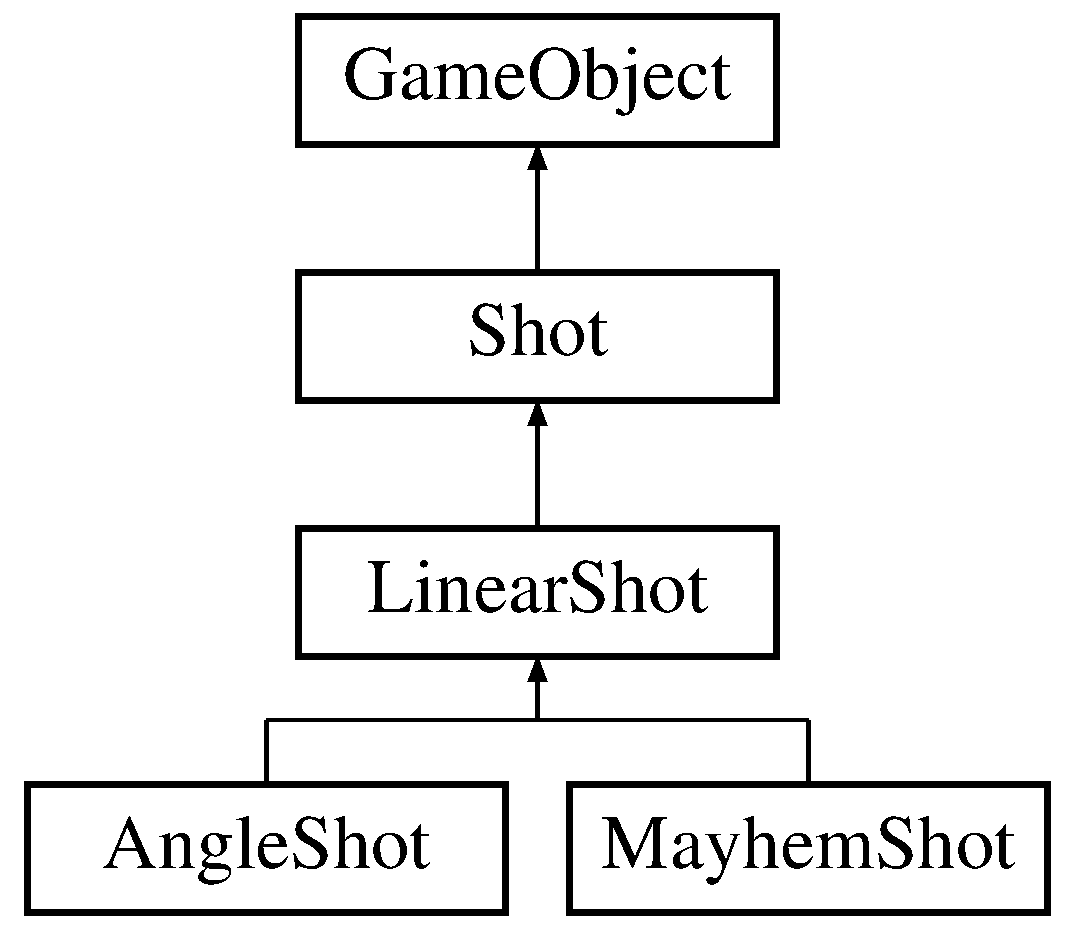
\includegraphics[height=4.000000cm]{class_linear_shot}
\end{center}
\end{figure}
\subsection*{Public Member Functions}
\begin{DoxyCompactItemize}
\item 
\hypertarget{class_linear_shot_a353b1988983a192affd6913805b8403e}{{\bfseries Linear\-Shot} (Q\-Rect p\-Rectangle, bool p\-To\-Up, int p\-Damage)}\label{class_linear_shot_a353b1988983a192affd6913805b8403e}

\item 
\hypertarget{class_linear_shot_af5e24419776495f3b42381fe614a3bec}{bool {\bfseries is\-Useful\-Shot} (Q\-Rect p\-Area)}\label{class_linear_shot_af5e24419776495f3b42381fe614a3bec}

\item 
bool \hyperlink{class_linear_shot_a5f74863ef2fe90a8e524945737029e0a}{is\-Collide} (\hyperlink{class_game_object}{Game\-Object} $\ast$other\-Renderizable)
\begin{DoxyCompactList}\small\item\em Verifica si un \hyperlink{class_game_object}{Game\-Object} esta colisionando con otro. \end{DoxyCompactList}\item 
\hypertarget{class_linear_shot_a9f7b9d654314185d6d89c8c24a64bc85}{int {\bfseries get\-X\-Velocity} ()}\label{class_linear_shot_a9f7b9d654314185d6d89c8c24a64bc85}

\item 
\hypertarget{class_linear_shot_ad0b2c8f2e67c4c8bf48895616c9f5683}{int {\bfseries get\-Y\-Velocity} ()}\label{class_linear_shot_ad0b2c8f2e67c4c8bf48895616c9f5683}

\item 
\hypertarget{class_linear_shot_a50717d095ffb35f445f909f0ef961a5a}{int {\bfseries get\-Type} ()}\label{class_linear_shot_a50717d095ffb35f445f909f0ef961a5a}

\item 
\hypertarget{class_linear_shot_a7f0ae98813020ba9c1860f24750b6fcf}{void \hyperlink{class_linear_shot_a7f0ae98813020ba9c1860f24750b6fcf}{update} ()}\label{class_linear_shot_a7f0ae98813020ba9c1860f24750b6fcf}

\begin{DoxyCompactList}\small\item\em Actualiza el objeto, es un metodo abstracto, y debe ser implementado por sus clases hijas. \end{DoxyCompactList}\end{DoxyCompactItemize}
\subsection*{Protected Attributes}
\begin{DoxyCompactItemize}
\item 
\hypertarget{class_linear_shot_a07e655ed82603f917e1d84758871f5bd}{int {\bfseries \-\_\-\-Velocity\-Y}}\label{class_linear_shot_a07e655ed82603f917e1d84758871f5bd}

\item 
\hypertarget{class_linear_shot_add140652fdd02d964e8827559d83a8ac}{bool {\bfseries \-\_\-\-Is\-Touched}}\label{class_linear_shot_add140652fdd02d964e8827559d83a8ac}

\end{DoxyCompactItemize}
\subsection*{Additional Inherited Members}


\subsection{Member Function Documentation}
\hypertarget{class_linear_shot_a5f74863ef2fe90a8e524945737029e0a}{\index{Linear\-Shot@{Linear\-Shot}!is\-Collide@{is\-Collide}}
\index{is\-Collide@{is\-Collide}!LinearShot@{Linear\-Shot}}
\subsubsection[{is\-Collide}]{\setlength{\rightskip}{0pt plus 5cm}bool Linear\-Shot\-::is\-Collide (
\begin{DoxyParamCaption}
\item[{{\bf Game\-Object} $\ast$}]{\-\_\-other\-Renderizable}
\end{DoxyParamCaption}
)\hspace{0.3cm}{\ttfamily [virtual]}}}\label{class_linear_shot_a5f74863ef2fe90a8e524945737029e0a}


Verifica si un \hyperlink{class_game_object}{Game\-Object} esta colisionando con otro. 


\begin{DoxyParams}{Parameters}
{\em \-\_\-other\-Renderizable} & el otro objeto para verificar que se colisione \\
\hline
\end{DoxyParams}
\begin{DoxyReturn}{Returns}
true si colisionan 
\end{DoxyReturn}


Reimplemented from \hyperlink{class_game_object_a4d7f7506ab6fa6442367844cd8202fb6}{Game\-Object}.



The documentation for this class was generated from the following files\-:\begin{DoxyCompactItemize}
\item 
logic/shot/linearshot.\-h\item 
logic/shot/linearshot.\-cpp\end{DoxyCompactItemize}

\hypertarget{class_linear_shot_fabric}{\section{Linear\-Shot\-Fabric Class Reference}
\label{class_linear_shot_fabric}\index{Linear\-Shot\-Fabric@{Linear\-Shot\-Fabric}}
}
Inheritance diagram for Linear\-Shot\-Fabric\-:\begin{figure}[H]
\begin{center}
\leavevmode
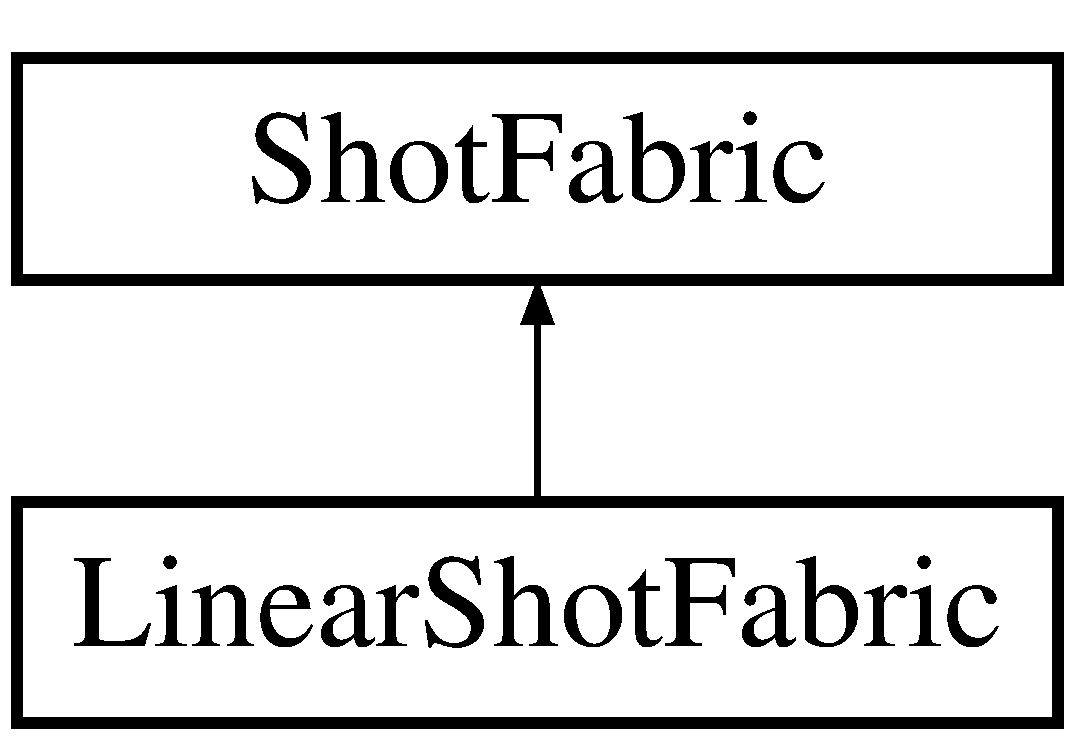
\includegraphics[height=2.000000cm]{class_linear_shot_fabric}
\end{center}
\end{figure}
\subsection*{Public Member Functions}
\begin{DoxyCompactItemize}
\item 
\hypertarget{class_linear_shot_fabric_a8e49b3e5c9930d996ceff1544d7deed4}{{\bfseries Linear\-Shot\-Fabric} (int p\-Max\-Munition)}\label{class_linear_shot_fabric_a8e49b3e5c9930d996ceff1544d7deed4}

\item 
\hypertarget{class_linear_shot_fabric_a62f5fd67da6fa1c985671a122e35f3fd}{\hyperlink{class_shot}{Shot} $\ast$ {\bfseries get\-New\-Shoot} (int p\-X, int p\-Y, bool p\-Player)}\label{class_linear_shot_fabric_a62f5fd67da6fa1c985671a122e35f3fd}

\item 
\hypertarget{class_linear_shot_fabric_a395b22701c39f96c4ff5ccd038c552d0}{int {\bfseries get\-Munition\-Type} ()}\label{class_linear_shot_fabric_a395b22701c39f96c4ff5ccd038c552d0}

\end{DoxyCompactItemize}
\subsection*{Additional Inherited Members}


The documentation for this class was generated from the following files\-:\begin{DoxyCompactItemize}
\item 
logic/shot/linearshotfabric.\-h\item 
logic/shot/linearshotfabric.\-cpp\end{DoxyCompactItemize}

\hypertarget{class_list}{\section{List$<$ E $>$ Class Template Reference}
\label{class_list}\index{List$<$ E $>$@{List$<$ E $>$}}
}


Esta clase es una estructura de datos especificamente una lista enlazada simple que puede contener cualquier tipo de dato solamente definiciendolo mediante el template de esta clase. se puede agregar y borrar el dato.  




{\ttfamily \#include $<$List.\-h$>$}

Inheritance diagram for List$<$ E $>$\-:\begin{figure}[H]
\begin{center}
\leavevmode
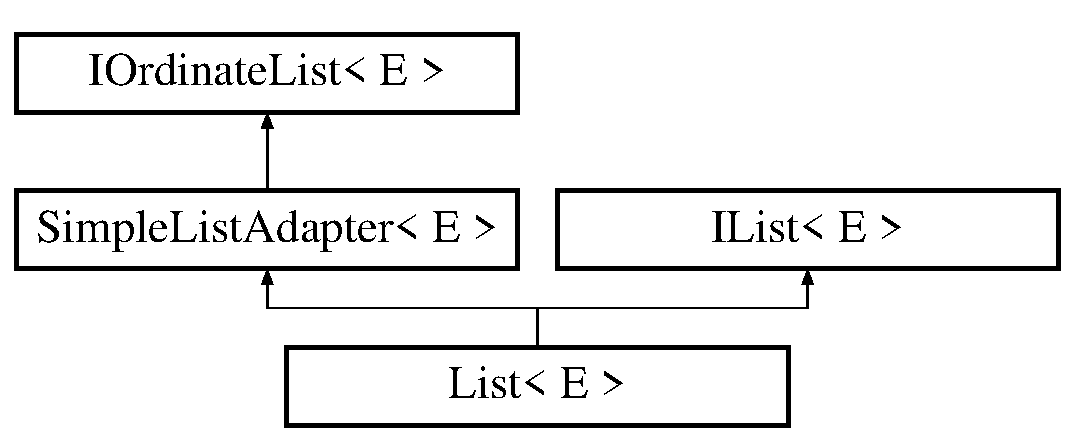
\includegraphics[height=3.000000cm]{class_list}
\end{center}
\end{figure}
\subsection*{Public Member Functions}
\begin{DoxyCompactItemize}
\item 
\hyperlink{class_list_ae47afd06bd8c39fe7a12d4489998e7c5}{List} ()
\begin{DoxyCompactList}\small\item\em Es el constructor de la lista. \end{DoxyCompactList}\item 
void \hyperlink{class_list_a4f0fb366c1153a4fd01826e9e6de5afc}{addi} (E)
\begin{DoxyCompactList}\small\item\em Agrega un elemento al principio de la lista. \end{DoxyCompactList}\item 
void \hyperlink{class_list_a2a130b7bc38cd968136f1f847e42d0cc}{add} (E)
\begin{DoxyCompactList}\small\item\em Agregar un elemento al final de la lista. \end{DoxyCompactList}\item 
bool \hyperlink{class_list_a530267346ebec244900c162de6f467e1}{add} (E, int)
\begin{DoxyCompactList}\small\item\em Agrega el elemento en el indice indicado. Si el indice es incorrecto no se agrega el elemento. \end{DoxyCompactList}\item 
bool \hyperlink{class_list_a46cec78299d3e23469276adf46adf9c1}{remove} (int)
\begin{DoxyCompactList}\small\item\em Remueve el dato en la posicion indicada por el parametro, en caso que el indice indicado sea incorrecto, osea que sea menor que cero o mayor o igual que el largo de la lista no alterara la lista. \end{DoxyCompactList}\item 
void \hyperlink{class_list_ac8b31be96806bd56f655436629ac2e7a}{set} (int, E)
\begin{DoxyCompactList}\small\item\em Setea el valor del dato que se encuentre en el indice citado con un nuevo valor. \end{DoxyCompactList}\item 
E \hyperlink{class_list_ab081a52d7a62aa6c5550ff9762f9427f}{get} (int)
\begin{DoxyCompactList}\small\item\em Obtiene un dato el la posicion indicada. En caso que el indice indicado sea incorrecto, osea que sea menor que cero o mayor o igual que el largo de la lista arrojara un error pues el dato esta fuera de los limites de la lista. \end{DoxyCompactList}\item 
\hyperlink{class_simple_iterator}{Simple\-Iterator}$<$ E $>$ $\ast$ \hyperlink{class_list_accb5fe71cb60ba7bf0ccab362b1f87cb}{get\-Iterator} ()
\begin{DoxyCompactList}\small\item\em Obtiene una instancia de un nuevo iterador de esta lista, y pueden obtenerse cuantas sean necesarias. pero es responsabilidad del programador eliminar mediante la palabra reservada delete. \end{DoxyCompactList}\item 
virtual \hyperlink{class_list_a0af4c4d8a3d0710e58b12db35f9b0a3d}{$\sim$\-List} ()
\begin{DoxyCompactList}\small\item\em Es el destructor de la lista. \end{DoxyCompactList}\item 
\hyperlink{class_list_ae47afd06bd8c39fe7a12d4489998e7c5}{List} ()
\end{DoxyCompactItemize}
\subsection*{Protected Member Functions}
\begin{DoxyCompactItemize}
\item 
bool \hyperlink{class_list_a92ad933f8d3a033b84a517fb6cc4111a}{addi} (E p\-Data)
\begin{DoxyCompactList}\small\item\em Agrega un elemento al principio de la lista. \end{DoxyCompactList}\item 
bool \hyperlink{class_list_a3c920f9c86d2853121c5cd2fb46f8436}{addf} (E p\-Data)
\item 
bool \hyperlink{class_list_ac38635d10f3faaf49af53c0b66347d0f}{add\-First\-Data} (E p\-Data)
\item 
bool \hyperlink{class_list_a1d0a5649ddd83cb781174698f80b2e0f}{removei} ()
\item 
bool \hyperlink{class_list_a45231b54bf8c98948becddd0923be138}{removef} ()
\end{DoxyCompactItemize}
\subsection*{Additional Inherited Members}


\subsection{Detailed Description}
\subsubsection*{template$<$class E$>$class List$<$ E $>$}

Esta clase es una estructura de datos especificamente una lista enlazada simple que puede contener cualquier tipo de dato solamente definiciendolo mediante el template de esta clase. se puede agregar y borrar el dato. 

\subsection{Constructor \& Destructor Documentation}
\hypertarget{class_list_ae47afd06bd8c39fe7a12d4489998e7c5}{\index{List@{List}!List@{List}}
\index{List@{List}!List@{List}}
\subsubsection[{List}]{\setlength{\rightskip}{0pt plus 5cm}template$<$class E $>$ {\bf List}$<$ E $>$\-::{\bf List} (
\begin{DoxyParamCaption}
{}
\end{DoxyParamCaption}
)}}\label{class_list_ae47afd06bd8c39fe7a12d4489998e7c5}


Es el constructor de la lista. 

\hypertarget{class_list_a0af4c4d8a3d0710e58b12db35f9b0a3d}{\index{List@{List}!$\sim$\-List@{$\sim$\-List}}
\index{$\sim$\-List@{$\sim$\-List}!List@{List}}
\subsubsection[{$\sim$\-List}]{\setlength{\rightskip}{0pt plus 5cm}template$<$class E $>$ {\bf List}$<$ E $>$\-::$\sim${\bf List} (
\begin{DoxyParamCaption}
{}
\end{DoxyParamCaption}
)\hspace{0.3cm}{\ttfamily [virtual]}}}\label{class_list_a0af4c4d8a3d0710e58b12db35f9b0a3d}


Es el destructor de la lista. 

\hypertarget{class_list_ae47afd06bd8c39fe7a12d4489998e7c5}{\index{List@{List}!List@{List}}
\index{List@{List}!List@{List}}
\subsubsection[{List}]{\setlength{\rightskip}{0pt plus 5cm}template$<$class E$>$ {\bf List}$<$ E $>$\-::{\bf List} (
\begin{DoxyParamCaption}
{}
\end{DoxyParamCaption}
)}}\label{class_list_ae47afd06bd8c39fe7a12d4489998e7c5}


\subsection{Member Function Documentation}
\hypertarget{class_list_a2a130b7bc38cd968136f1f847e42d0cc}{\index{List@{List}!add@{add}}
\index{add@{add}!List@{List}}
\subsubsection[{add}]{\setlength{\rightskip}{0pt plus 5cm}template$<$class E$>$ void {\bf List}$<$ E $>$\-::add (
\begin{DoxyParamCaption}
\item[{E}]{data}
\end{DoxyParamCaption}
)\hspace{0.3cm}{\ttfamily [virtual]}}}\label{class_list_a2a130b7bc38cd968136f1f847e42d0cc}


Agregar un elemento al final de la lista. 


\begin{DoxyParams}{Parameters}
{\em data} & el elemento a agregar \\
\hline
\end{DoxyParams}


Implements \hyperlink{class_i_list_a27500caa3d9da05aa6437d5ff56b09e2}{I\-List$<$ E $>$}.

\hypertarget{class_list_a530267346ebec244900c162de6f467e1}{\index{List@{List}!add@{add}}
\index{add@{add}!List@{List}}
\subsubsection[{add}]{\setlength{\rightskip}{0pt plus 5cm}template$<$class E$>$ bool {\bf List}$<$ E $>$\-::add (
\begin{DoxyParamCaption}
\item[{E}]{data, }
\item[{int}]{index}
\end{DoxyParamCaption}
)\hspace{0.3cm}{\ttfamily [virtual]}}}\label{class_list_a530267346ebec244900c162de6f467e1}


Agrega el elemento en el indice indicado. Si el indice es incorrecto no se agrega el elemento. 


\begin{DoxyParams}{Parameters}
{\em dato} & el elemento a agregar \\
\hline
{\em index} & el indice que indica el lugar donde se agregara \\
\hline
\end{DoxyParams}
\begin{DoxyReturn}{Returns}
si el elemento se agrega retorna true, en caso contrario retorna false 
\end{DoxyReturn}


Implements \hyperlink{class_i_list_a70140dbc9de2b9f6e5ffd2212d5ea8b0}{I\-List$<$ E $>$}.

\hypertarget{class_list_a3c920f9c86d2853121c5cd2fb46f8436}{\index{List@{List}!addf@{addf}}
\index{addf@{addf}!List@{List}}
\subsubsection[{addf}]{\setlength{\rightskip}{0pt plus 5cm}template$<$class E$>$ bool {\bf List}$<$ E $>$\-::addf (
\begin{DoxyParamCaption}
\item[{E}]{p\-Data}
\end{DoxyParamCaption}
)\hspace{0.3cm}{\ttfamily [protected]}, {\ttfamily [virtual]}}}\label{class_list_a3c920f9c86d2853121c5cd2fb46f8436}


Implements \hyperlink{class_simple_list_adapter_a89d3c954a3782181f871b30c7a726379}{Simple\-List\-Adapter$<$ E $>$}.

\hypertarget{class_list_ac38635d10f3faaf49af53c0b66347d0f}{\index{List@{List}!add\-First\-Data@{add\-First\-Data}}
\index{add\-First\-Data@{add\-First\-Data}!List@{List}}
\subsubsection[{add\-First\-Data}]{\setlength{\rightskip}{0pt plus 5cm}template$<$class E$>$ bool {\bf List}$<$ E $>$\-::add\-First\-Data (
\begin{DoxyParamCaption}
\item[{E}]{p\-Data}
\end{DoxyParamCaption}
)\hspace{0.3cm}{\ttfamily [protected]}, {\ttfamily [virtual]}}}\label{class_list_ac38635d10f3faaf49af53c0b66347d0f}


Implements \hyperlink{class_simple_list_adapter_a269a73b10beb87dddb3330af47334522}{Simple\-List\-Adapter$<$ E $>$}.

\hypertarget{class_list_a92ad933f8d3a033b84a517fb6cc4111a}{\index{List@{List}!addi@{addi}}
\index{addi@{addi}!List@{List}}
\subsubsection[{addi}]{\setlength{\rightskip}{0pt plus 5cm}template$<$class E$>$ bool {\bf List}$<$ E $>$\-::addi (
\begin{DoxyParamCaption}
\item[{E}]{}
\end{DoxyParamCaption}
)\hspace{0.3cm}{\ttfamily [protected]}, {\ttfamily [virtual]}}}\label{class_list_a92ad933f8d3a033b84a517fb6cc4111a}


Agrega un elemento al principio de la lista. 


\begin{DoxyParams}{Parameters}
{\em data} & el elemento a agregar \\
\hline
\end{DoxyParams}


Implements \hyperlink{class_i_list_af202dc9e748ee32238d80e57dfbcae20}{I\-List$<$ E $>$}.

\hypertarget{class_list_a4f0fb366c1153a4fd01826e9e6de5afc}{\index{List@{List}!addi@{addi}}
\index{addi@{addi}!List@{List}}
\subsubsection[{addi}]{\setlength{\rightskip}{0pt plus 5cm}template$<$class E$>$ bool {\bf List}$<$ E $>$\-::addi (
\begin{DoxyParamCaption}
\item[{E}]{data}
\end{DoxyParamCaption}
)\hspace{0.3cm}{\ttfamily [virtual]}}}\label{class_list_a4f0fb366c1153a4fd01826e9e6de5afc}


Agrega un elemento al principio de la lista. 


\begin{DoxyParams}{Parameters}
{\em data} & el elemento a agregar \\
\hline
\end{DoxyParams}


Implements \hyperlink{class_i_list_af202dc9e748ee32238d80e57dfbcae20}{I\-List$<$ E $>$}.

\hypertarget{class_list_ab081a52d7a62aa6c5550ff9762f9427f}{\index{List@{List}!get@{get}}
\index{get@{get}!List@{List}}
\subsubsection[{get}]{\setlength{\rightskip}{0pt plus 5cm}template$<$class E $>$ E {\bf List}$<$ E $>$\-::get (
\begin{DoxyParamCaption}
\item[{int}]{index}
\end{DoxyParamCaption}
)\hspace{0.3cm}{\ttfamily [virtual]}}}\label{class_list_ab081a52d7a62aa6c5550ff9762f9427f}


Obtiene un dato el la posicion indicada. En caso que el indice indicado sea incorrecto, osea que sea menor que cero o mayor o igual que el largo de la lista arrojara un error pues el dato esta fuera de los limites de la lista. 


\begin{DoxyParams}{Parameters}
{\em index} & el indice indicado \\
\hline
\end{DoxyParams}
\begin{DoxyReturn}{Returns}
E el dato buscado por el indice indicado 
\end{DoxyReturn}

\begin{DoxyExceptions}{Exceptions}
{\em indexoutbounds} & fuera de rango \\
\hline
\end{DoxyExceptions}


Implements \hyperlink{class_i_list_a60570f7ee0e7474d01b2f364bad996a0}{I\-List$<$ E $>$}.

\hypertarget{class_list_accb5fe71cb60ba7bf0ccab362b1f87cb}{\index{List@{List}!get\-Iterator@{get\-Iterator}}
\index{get\-Iterator@{get\-Iterator}!List@{List}}
\subsubsection[{get\-Iterator}]{\setlength{\rightskip}{0pt plus 5cm}template$<$class E $>$ {\bf Simple\-Iterator}$<$ E $>$ $\ast$ {\bf List}$<$ E $>$\-::get\-Iterator (
\begin{DoxyParamCaption}
{}
\end{DoxyParamCaption}
)\hspace{0.3cm}{\ttfamily [virtual]}}}\label{class_list_accb5fe71cb60ba7bf0ccab362b1f87cb}


Obtiene una instancia de un nuevo iterador de esta lista, y pueden obtenerse cuantas sean necesarias. pero es responsabilidad del programador eliminar mediante la palabra reservada delete. 

\begin{DoxyReturn}{Returns}
I\-Iterator$<$\-E$>$ un puntero de0l iterador indicado 
\end{DoxyReturn}


Implements \hyperlink{class_i_list_a997815664cc6b20eb5dfa9968251d2cd}{I\-List$<$ E $>$}.

\hypertarget{class_list_a46cec78299d3e23469276adf46adf9c1}{\index{List@{List}!remove@{remove}}
\index{remove@{remove}!List@{List}}
\subsubsection[{remove}]{\setlength{\rightskip}{0pt plus 5cm}template$<$class E $>$ bool {\bf List}$<$ E $>$\-::remove (
\begin{DoxyParamCaption}
\item[{int}]{index}
\end{DoxyParamCaption}
)\hspace{0.3cm}{\ttfamily [virtual]}}}\label{class_list_a46cec78299d3e23469276adf46adf9c1}


Remueve el dato en la posicion indicada por el parametro, en caso que el indice indicado sea incorrecto, osea que sea menor que cero o mayor o igual que el largo de la lista no alterara la lista. 


\begin{DoxyParams}{Parameters}
{\em index} & la posicion indicada del objeto a borrar \\
\hline
\end{DoxyParams}
\begin{DoxyReturn}{Returns}
true si borra algo, false si el indice indicado es incorrecto 
\end{DoxyReturn}


Implements \hyperlink{class_i_list_a9bf7d737252dfbd4c9a5d7be36ea4231}{I\-List$<$ E $>$}.

\hypertarget{class_list_a45231b54bf8c98948becddd0923be138}{\index{List@{List}!removef@{removef}}
\index{removef@{removef}!List@{List}}
\subsubsection[{removef}]{\setlength{\rightskip}{0pt plus 5cm}template$<$class E $>$ bool {\bf List}$<$ E $>$\-::removef (
\begin{DoxyParamCaption}
{}
\end{DoxyParamCaption}
)\hspace{0.3cm}{\ttfamily [protected]}, {\ttfamily [virtual]}}}\label{class_list_a45231b54bf8c98948becddd0923be138}


Implements \hyperlink{class_simple_list_adapter_a9008dff51a5a156c0929b972e59e8f1d}{Simple\-List\-Adapter$<$ E $>$}.

\hypertarget{class_list_a1d0a5649ddd83cb781174698f80b2e0f}{\index{List@{List}!removei@{removei}}
\index{removei@{removei}!List@{List}}
\subsubsection[{removei}]{\setlength{\rightskip}{0pt plus 5cm}template$<$class E $>$ bool {\bf List}$<$ E $>$\-::removei (
\begin{DoxyParamCaption}
{}
\end{DoxyParamCaption}
)\hspace{0.3cm}{\ttfamily [protected]}, {\ttfamily [virtual]}}}\label{class_list_a1d0a5649ddd83cb781174698f80b2e0f}


Implements \hyperlink{class_simple_list_adapter_a9bebc8a42330e453f6e608e54de36adf}{Simple\-List\-Adapter$<$ E $>$}.

\hypertarget{class_list_ac8b31be96806bd56f655436629ac2e7a}{\index{List@{List}!set@{set}}
\index{set@{set}!List@{List}}
\subsubsection[{set}]{\setlength{\rightskip}{0pt plus 5cm}template$<$class E$>$ void {\bf List}$<$ E $>$\-::set (
\begin{DoxyParamCaption}
\item[{int}]{index, }
\item[{E}]{data}
\end{DoxyParamCaption}
)\hspace{0.3cm}{\ttfamily [virtual]}}}\label{class_list_ac8b31be96806bd56f655436629ac2e7a}


Setea el valor del dato que se encuentre en el indice citado con un nuevo valor. 


\begin{DoxyParams}{Parameters}
{\em int} & el indice en el que se encuetra el dato \\
\hline
{\em E} & el dato por el que se cambiara \\
\hline
\end{DoxyParams}


Implements \hyperlink{class_i_list_a119ed658d2804aec0b9fef9325c03073}{I\-List$<$ E $>$}.



The documentation for this class was generated from the following file\-:\begin{DoxyCompactItemize}
\item 
list/\hyperlink{_list_8h}{List.\-h}\end{DoxyCompactItemize}

\hypertarget{class_mayhem_shot}{\section{Mayhem\-Shot Class Reference}
\label{class_mayhem_shot}\index{Mayhem\-Shot@{Mayhem\-Shot}}
}


{\ttfamily \#include $<$mayhemshot.\-h$>$}

Inheritance diagram for Mayhem\-Shot\-:\begin{figure}[H]
\begin{center}
\leavevmode
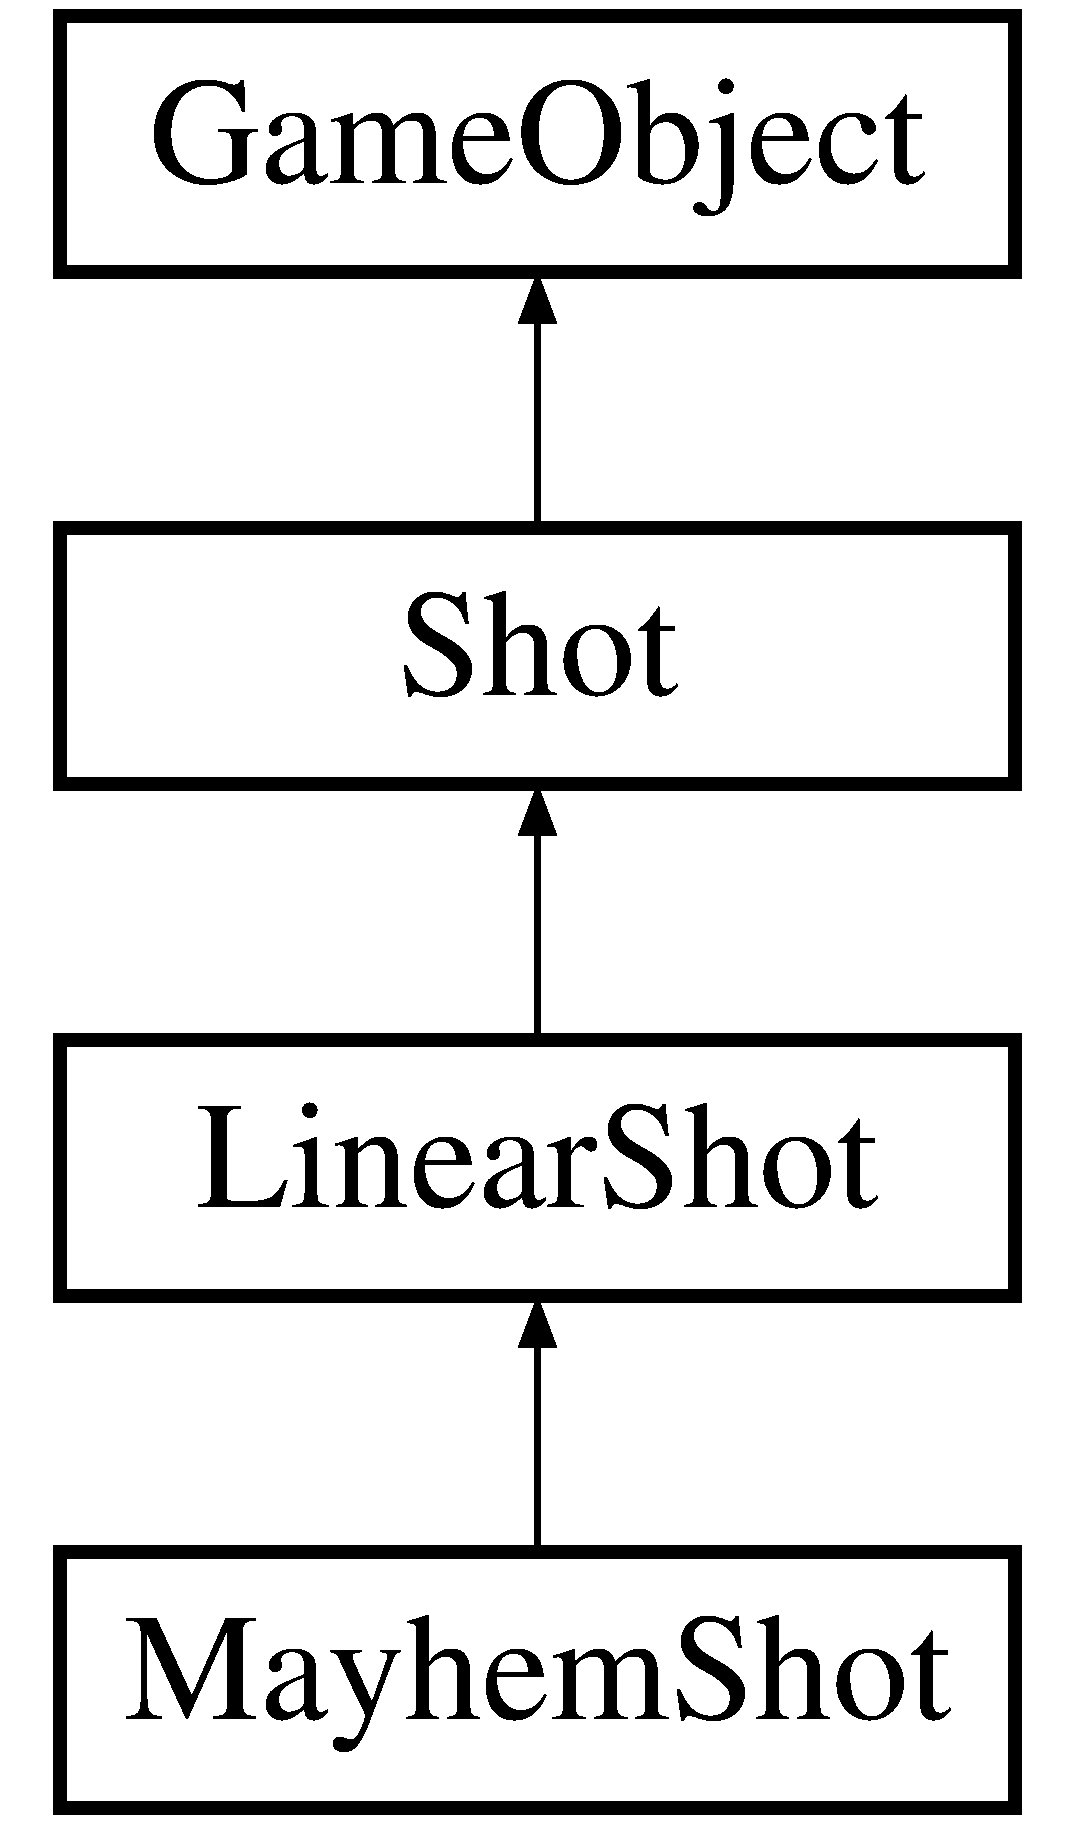
\includegraphics[height=4.000000cm]{class_mayhem_shot}
\end{center}
\end{figure}
\subsection*{Public Member Functions}
\begin{DoxyCompactItemize}
\item 
\hyperlink{class_mayhem_shot_a0f1115fcbf4c848347e7d9b91f36b730}{Mayhem\-Shot} (Q\-Rect p\-Rectangle, int p\-Damage)
\item 
void \hyperlink{class_mayhem_shot_aae8e9c0bcac2eddc50774decf0fd7c2e}{damage} (\hyperlink{class_h_p_entity}{H\-P\-Entity} $\ast$p\-Entity)
\item 
int \hyperlink{class_mayhem_shot_a2aa6e9bf2e931477ace1731d3eed0500}{get\-Type} ()
\item 
\hyperlink{class_mayhem_shot_aab33285dd353baa3895556e664a150c0}{$\sim$\-Mayhem\-Shot} ()
\end{DoxyCompactItemize}
\subsection*{Additional Inherited Members}


\subsection{Constructor \& Destructor Documentation}
\hypertarget{class_mayhem_shot_a0f1115fcbf4c848347e7d9b91f36b730}{\index{Mayhem\-Shot@{Mayhem\-Shot}!Mayhem\-Shot@{Mayhem\-Shot}}
\index{Mayhem\-Shot@{Mayhem\-Shot}!MayhemShot@{Mayhem\-Shot}}
\subsubsection[{Mayhem\-Shot}]{\setlength{\rightskip}{0pt plus 5cm}Mayhem\-Shot\-::\-Mayhem\-Shot (
\begin{DoxyParamCaption}
\item[{Q\-Rect}]{p\-Rectangle, }
\item[{int}]{p\-Damage}
\end{DoxyParamCaption}
)}}\label{class_mayhem_shot_a0f1115fcbf4c848347e7d9b91f36b730}
\hypertarget{class_mayhem_shot_aab33285dd353baa3895556e664a150c0}{\index{Mayhem\-Shot@{Mayhem\-Shot}!$\sim$\-Mayhem\-Shot@{$\sim$\-Mayhem\-Shot}}
\index{$\sim$\-Mayhem\-Shot@{$\sim$\-Mayhem\-Shot}!MayhemShot@{Mayhem\-Shot}}
\subsubsection[{$\sim$\-Mayhem\-Shot}]{\setlength{\rightskip}{0pt plus 5cm}Mayhem\-Shot\-::$\sim$\-Mayhem\-Shot (
\begin{DoxyParamCaption}
{}
\end{DoxyParamCaption}
)\hspace{0.3cm}{\ttfamily [inline]}}}\label{class_mayhem_shot_aab33285dd353baa3895556e664a150c0}


\subsection{Member Function Documentation}
\hypertarget{class_mayhem_shot_aae8e9c0bcac2eddc50774decf0fd7c2e}{\index{Mayhem\-Shot@{Mayhem\-Shot}!damage@{damage}}
\index{damage@{damage}!MayhemShot@{Mayhem\-Shot}}
\subsubsection[{damage}]{\setlength{\rightskip}{0pt plus 5cm}void Mayhem\-Shot\-::damage (
\begin{DoxyParamCaption}
\item[{{\bf H\-P\-Entity} $\ast$}]{p\-Entity}
\end{DoxyParamCaption}
)\hspace{0.3cm}{\ttfamily [virtual]}}}\label{class_mayhem_shot_aae8e9c0bcac2eddc50774decf0fd7c2e}


Reimplemented from \hyperlink{class_shot_a6f78a6d0f6e7e44619b0128c14ce5730}{Shot}.

\hypertarget{class_mayhem_shot_a2aa6e9bf2e931477ace1731d3eed0500}{\index{Mayhem\-Shot@{Mayhem\-Shot}!get\-Type@{get\-Type}}
\index{get\-Type@{get\-Type}!MayhemShot@{Mayhem\-Shot}}
\subsubsection[{get\-Type}]{\setlength{\rightskip}{0pt plus 5cm}int Mayhem\-Shot\-::get\-Type (
\begin{DoxyParamCaption}
{}
\end{DoxyParamCaption}
)\hspace{0.3cm}{\ttfamily [virtual]}}}\label{class_mayhem_shot_a2aa6e9bf2e931477ace1731d3eed0500}


Reimplemented from \hyperlink{class_linear_shot_a50717d095ffb35f445f909f0ef961a5a}{Linear\-Shot}.



The documentation for this class was generated from the following files\-:\begin{DoxyCompactItemize}
\item 
logic/shot/\hyperlink{mayhemshot_8h}{mayhemshot.\-h}\item 
logic/shot/\hyperlink{mayhemshot_8cpp}{mayhemshot.\-cpp}\end{DoxyCompactItemize}

\hypertarget{class_mayhem_shot_manager}{\section{Mayhem\-Shot\-Manager Class Reference}
\label{class_mayhem_shot_manager}\index{Mayhem\-Shot\-Manager@{Mayhem\-Shot\-Manager}}
}
Inheritance diagram for Mayhem\-Shot\-Manager\-:\begin{figure}[H]
\begin{center}
\leavevmode
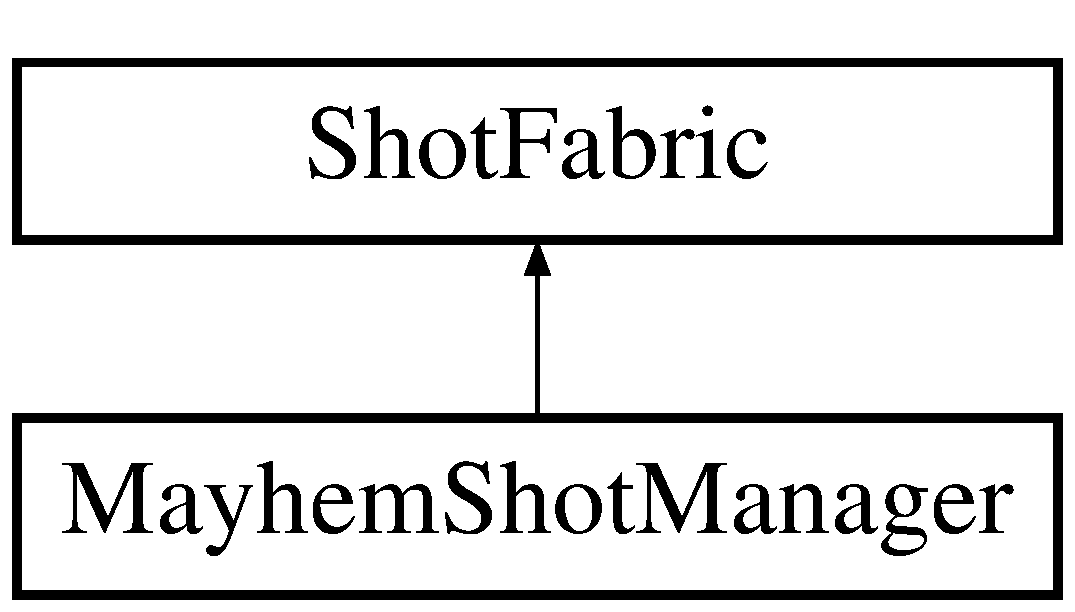
\includegraphics[height=2.000000cm]{class_mayhem_shot_manager}
\end{center}
\end{figure}
\subsection*{Public Member Functions}
\begin{DoxyCompactItemize}
\item 
\hypertarget{class_mayhem_shot_manager_a3be4a6716d2fc370643d97cfbba9e8a0}{{\bfseries Mayhem\-Shot\-Manager} (int p\-Max\-Munition)}\label{class_mayhem_shot_manager_a3be4a6716d2fc370643d97cfbba9e8a0}

\item 
\hypertarget{class_mayhem_shot_manager_ab55fb0975a345e534dfa34339511a7a1}{int {\bfseries get\-Munition\-Type} ()}\label{class_mayhem_shot_manager_ab55fb0975a345e534dfa34339511a7a1}

\item 
\hypertarget{class_mayhem_shot_manager_a184f651f761cc1fb19e8594f43cecfb3}{\hyperlink{class_shot}{Shot} $\ast$ {\bfseries get\-New\-Shoot} (int p\-X, int p\-Y, bool p\-Player)}\label{class_mayhem_shot_manager_a184f651f761cc1fb19e8594f43cecfb3}

\end{DoxyCompactItemize}
\subsection*{Additional Inherited Members}


The documentation for this class was generated from the following files\-:\begin{DoxyCompactItemize}
\item 
logic/shot/mayhemshotmanager.\-h\item 
logic/shot/mayhemshotmanager.\-cpp\end{DoxyCompactItemize}

\hypertarget{class_movil_enemy_rocket}{\section{Movil\-Enemy\-Rocket Class Reference}
\label{class_movil_enemy_rocket}\index{Movil\-Enemy\-Rocket@{Movil\-Enemy\-Rocket}}
}


{\ttfamily \#include $<$movilenemyrocket.\-h$>$}

Inheritance diagram for Movil\-Enemy\-Rocket\-:\begin{figure}[H]
\begin{center}
\leavevmode
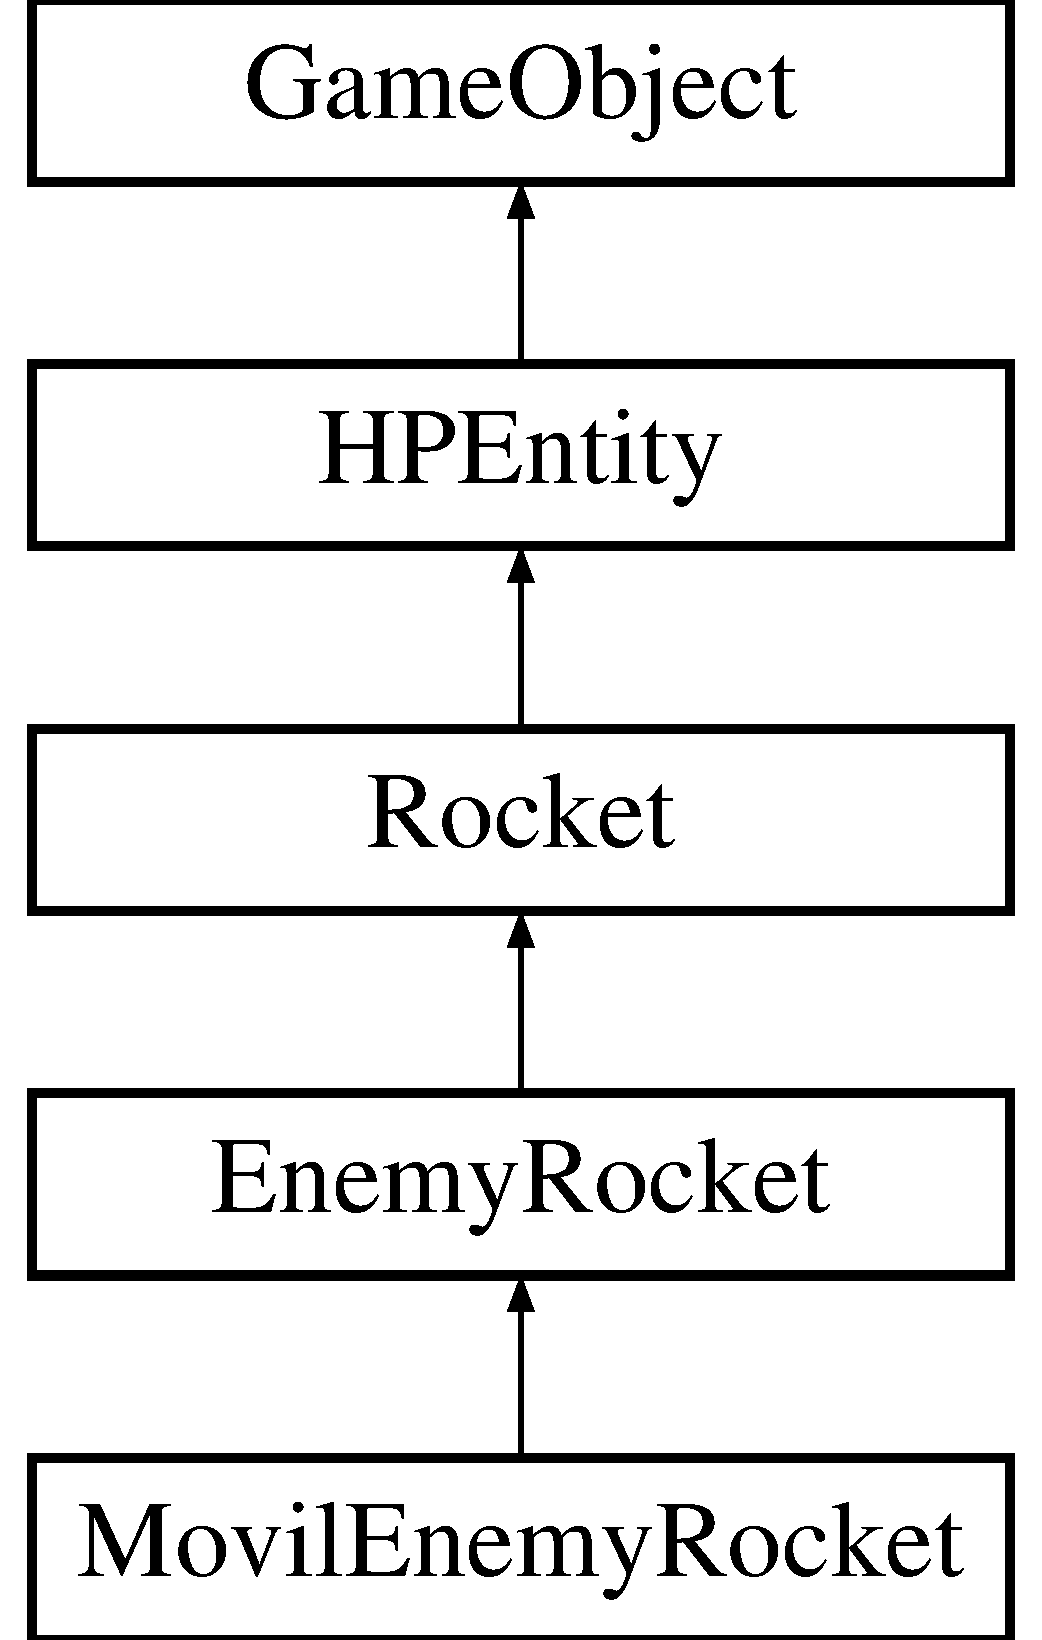
\includegraphics[height=5.000000cm]{class_movil_enemy_rocket}
\end{center}
\end{figure}
\subsection*{Public Member Functions}
\begin{DoxyCompactItemize}
\item 
\hyperlink{class_movil_enemy_rocket_a8108d2f9bec6a399e475e474beedf2ef}{Movil\-Enemy\-Rocket} (Q\-Rect p\-Rectangle, int p\-Max\-Hp)
\item 
int \hyperlink{class_movil_enemy_rocket_a6372ff2e56ce1494f3e3e2420706ef3e}{get\-Enemy\-Type} ()
\item 
void \hyperlink{class_movil_enemy_rocket_af18f4b9b815e7fe4a3817845a644df40}{update} ()
\begin{DoxyCompactList}\small\item\em Actualiza el objeto, es un metodo abstracto, y debe ser implementado por sus clases hijas. \end{DoxyCompactList}\end{DoxyCompactItemize}
\subsection*{Additional Inherited Members}


\subsection{Constructor \& Destructor Documentation}
\hypertarget{class_movil_enemy_rocket_a8108d2f9bec6a399e475e474beedf2ef}{\index{Movil\-Enemy\-Rocket@{Movil\-Enemy\-Rocket}!Movil\-Enemy\-Rocket@{Movil\-Enemy\-Rocket}}
\index{Movil\-Enemy\-Rocket@{Movil\-Enemy\-Rocket}!MovilEnemyRocket@{Movil\-Enemy\-Rocket}}
\subsubsection[{Movil\-Enemy\-Rocket}]{\setlength{\rightskip}{0pt plus 5cm}Movil\-Enemy\-Rocket\-::\-Movil\-Enemy\-Rocket (
\begin{DoxyParamCaption}
\item[{Q\-Rect}]{p\-Rectangle, }
\item[{int}]{p\-Max\-Hp}
\end{DoxyParamCaption}
)}}\label{class_movil_enemy_rocket_a8108d2f9bec6a399e475e474beedf2ef}


\subsection{Member Function Documentation}
\hypertarget{class_movil_enemy_rocket_a6372ff2e56ce1494f3e3e2420706ef3e}{\index{Movil\-Enemy\-Rocket@{Movil\-Enemy\-Rocket}!get\-Enemy\-Type@{get\-Enemy\-Type}}
\index{get\-Enemy\-Type@{get\-Enemy\-Type}!MovilEnemyRocket@{Movil\-Enemy\-Rocket}}
\subsubsection[{get\-Enemy\-Type}]{\setlength{\rightskip}{0pt plus 5cm}int Movil\-Enemy\-Rocket\-::get\-Enemy\-Type (
\begin{DoxyParamCaption}
{}
\end{DoxyParamCaption}
)\hspace{0.3cm}{\ttfamily [virtual]}}}\label{class_movil_enemy_rocket_a6372ff2e56ce1494f3e3e2420706ef3e}


Implements \hyperlink{class_enemy_rocket_a44e857f29c0846545743e21638391527}{Enemy\-Rocket}.

\hypertarget{class_movil_enemy_rocket_af18f4b9b815e7fe4a3817845a644df40}{\index{Movil\-Enemy\-Rocket@{Movil\-Enemy\-Rocket}!update@{update}}
\index{update@{update}!MovilEnemyRocket@{Movil\-Enemy\-Rocket}}
\subsubsection[{update}]{\setlength{\rightskip}{0pt plus 5cm}void Movil\-Enemy\-Rocket\-::update (
\begin{DoxyParamCaption}
{}
\end{DoxyParamCaption}
)\hspace{0.3cm}{\ttfamily [virtual]}}}\label{class_movil_enemy_rocket_af18f4b9b815e7fe4a3817845a644df40}


Actualiza el objeto, es un metodo abstracto, y debe ser implementado por sus clases hijas. 



Implements \hyperlink{class_game_object_ae83128d0e0efef691417779605ee037c}{Game\-Object}.



The documentation for this class was generated from the following files\-:\begin{DoxyCompactItemize}
\item 
logic/rocket/\hyperlink{movilenemyrocket_8h}{movilenemyrocket.\-h}\item 
logic/rocket/\hyperlink{movilenemyrocket_8cpp}{movilenemyrocket.\-cpp}\end{DoxyCompactItemize}

\hypertarget{class_node}{\section{Node$<$ E $>$ Class Template Reference}
\label{class_node}\index{Node$<$ E $>$@{Node$<$ E $>$}}
}


Es la parte elemental de una lista simple.  




{\ttfamily \#include $<$Node.\-h$>$}

\subsection*{Public Member Functions}
\begin{DoxyCompactItemize}
\item 
\hyperlink{class_node_a74d41f93c30d8c3036d24894f0e4314e}{Node} (E)
\begin{DoxyCompactList}\small\item\em Constructor del Nodo, el next se setea como un puntero nulo para evitar punteros colgados. \end{DoxyCompactList}\item 
\hyperlink{class_node_adc1b4c81c3fb6d0580f138650629a41e}{Node} (E data, \hyperlink{class_node}{Node}$<$ E $>$ $\ast$next)
\begin{DoxyCompactList}\small\item\em Constructor del Nodo. \end{DoxyCompactList}\item 
void \hyperlink{class_node_ae13418a552fa36eddbaa5dfb767aa664}{set\-Data} (E)
\begin{DoxyCompactList}\small\item\em Setea el dato contenido en el nodo. \end{DoxyCompactList}\item 
E \hyperlink{class_node_a02a4e5126542aaa1a2150932cfa2b8ce}{get\-Data} () const 
\begin{DoxyCompactList}\small\item\em Obtiene el dato contenido en el nodo. \end{DoxyCompactList}\item 
\hypertarget{class_node_adec417c9f6f7d2cbd0fc7a72508e9c3d}{E \& {\bfseries get\-Reference\-Data} ()}\label{class_node_adec417c9f6f7d2cbd0fc7a72508e9c3d}

\item 
void \hyperlink{class_node_a2ce12b4f2605972720e1c56fe80014a0}{set\-Next} (\hyperlink{class_node}{Node}$<$ E $>$ $\ast$)
\begin{DoxyCompactList}\small\item\em Setea el puntero del nodo siguiente. \end{DoxyCompactList}\item 
\hyperlink{class_node}{Node}$<$ E $>$ $\ast$ \hyperlink{class_node_aeb063e5172867e988550ab7d6c280db7}{get\-Next} () const 
\begin{DoxyCompactList}\small\item\em Obtiene el nodo siguiente. \end{DoxyCompactList}\item 
\hypertarget{class_node_af907944256d9fca41c6a1c783a3a6536}{virtual \hyperlink{class_node_af907944256d9fca41c6a1c783a3a6536}{$\sim$\-Node} ()}\label{class_node_af907944256d9fca41c6a1c783a3a6536}

\begin{DoxyCompactList}\small\item\em Liberador de memoria. \end{DoxyCompactList}\end{DoxyCompactItemize}


\subsection{Detailed Description}
\subsubsection*{template$<$class E$>$class Node$<$ E $>$}

Es la parte elemental de una lista simple. 

\subsection{Constructor \& Destructor Documentation}
\hypertarget{class_node_a74d41f93c30d8c3036d24894f0e4314e}{\index{Node@{Node}!Node@{Node}}
\index{Node@{Node}!Node@{Node}}
\subsubsection[{Node}]{\setlength{\rightskip}{0pt plus 5cm}template$<$class E$>$ {\bf Node}$<$ E $>$\-::{\bf Node} (
\begin{DoxyParamCaption}
\item[{E}]{data}
\end{DoxyParamCaption}
)}}\label{class_node_a74d41f93c30d8c3036d24894f0e4314e}


Constructor del Nodo, el next se setea como un puntero nulo para evitar punteros colgados. 


\begin{DoxyParams}{Parameters}
{\em data} & el dato que contrendra el nodo \\
\hline
\end{DoxyParams}
\hypertarget{class_node_adc1b4c81c3fb6d0580f138650629a41e}{\index{Node@{Node}!Node@{Node}}
\index{Node@{Node}!Node@{Node}}
\subsubsection[{Node}]{\setlength{\rightskip}{0pt plus 5cm}template$<$class E$>$ {\bf Node}$<$ E $>$\-::{\bf Node} (
\begin{DoxyParamCaption}
\item[{E}]{data, }
\item[{{\bf Node}$<$ E $>$ $\ast$}]{next}
\end{DoxyParamCaption}
)}}\label{class_node_adc1b4c81c3fb6d0580f138650629a41e}


Constructor del Nodo. 


\begin{DoxyParams}{Parameters}
{\em data} & el dato que contendra el dato \\
\hline
{\em next} & el puntero al nodo siguiente \\
\hline
\end{DoxyParams}


\subsection{Member Function Documentation}
\hypertarget{class_node_a02a4e5126542aaa1a2150932cfa2b8ce}{\index{Node@{Node}!get\-Data@{get\-Data}}
\index{get\-Data@{get\-Data}!Node@{Node}}
\subsubsection[{get\-Data}]{\setlength{\rightskip}{0pt plus 5cm}template$<$class E $>$ E {\bf Node}$<$ E $>$\-::get\-Data (
\begin{DoxyParamCaption}
{}
\end{DoxyParamCaption}
) const}}\label{class_node_a02a4e5126542aaa1a2150932cfa2b8ce}


Obtiene el dato contenido en el nodo. 

\begin{DoxyReturn}{Returns}
E el dato contenido 
\end{DoxyReturn}
\hypertarget{class_node_aeb063e5172867e988550ab7d6c280db7}{\index{Node@{Node}!get\-Next@{get\-Next}}
\index{get\-Next@{get\-Next}!Node@{Node}}
\subsubsection[{get\-Next}]{\setlength{\rightskip}{0pt plus 5cm}template$<$class E $>$ {\bf Node}$<$ E $>$ $\ast$ {\bf Node}$<$ E $>$\-::get\-Next (
\begin{DoxyParamCaption}
{}
\end{DoxyParamCaption}
) const}}\label{class_node_aeb063e5172867e988550ab7d6c280db7}


Obtiene el nodo siguiente. 

\begin{DoxyReturn}{Returns}
Double\-Node$<$\-E$>$ el nodo siguiente 
\end{DoxyReturn}
\hypertarget{class_node_ae13418a552fa36eddbaa5dfb767aa664}{\index{Node@{Node}!set\-Data@{set\-Data}}
\index{set\-Data@{set\-Data}!Node@{Node}}
\subsubsection[{set\-Data}]{\setlength{\rightskip}{0pt plus 5cm}template$<$class E$>$ void {\bf Node}$<$ E $>$\-::set\-Data (
\begin{DoxyParamCaption}
\item[{E}]{data}
\end{DoxyParamCaption}
)}}\label{class_node_ae13418a552fa36eddbaa5dfb767aa664}


Setea el dato contenido en el nodo. 


\begin{DoxyParams}{Parameters}
{\em data} & el dato nuevo \\
\hline
\end{DoxyParams}
\hypertarget{class_node_a2ce12b4f2605972720e1c56fe80014a0}{\index{Node@{Node}!set\-Next@{set\-Next}}
\index{set\-Next@{set\-Next}!Node@{Node}}
\subsubsection[{set\-Next}]{\setlength{\rightskip}{0pt plus 5cm}template$<$class E$>$ void {\bf Node}$<$ E $>$\-::set\-Next (
\begin{DoxyParamCaption}
\item[{{\bf Node}$<$ E $>$ $\ast$}]{next}
\end{DoxyParamCaption}
)}}\label{class_node_a2ce12b4f2605972720e1c56fe80014a0}


Setea el puntero del nodo siguiente. 


\begin{DoxyParams}{Parameters}
{\em next} & el nuevo nodo que representa el nodo siguiente \\
\hline
\end{DoxyParams}


The documentation for this class was generated from the following file\-:\begin{DoxyCompactItemize}
\item 
list/Node.\-h\end{DoxyCompactItemize}

\hypertarget{class_observer}{\section{Observer Class Reference}
\label{class_observer}\index{Observer@{Observer}}
}


{\ttfamily \#include $<$observer.\-h$>$}

Inheritance diagram for Observer\-:\begin{figure}[H]
\begin{center}
\leavevmode
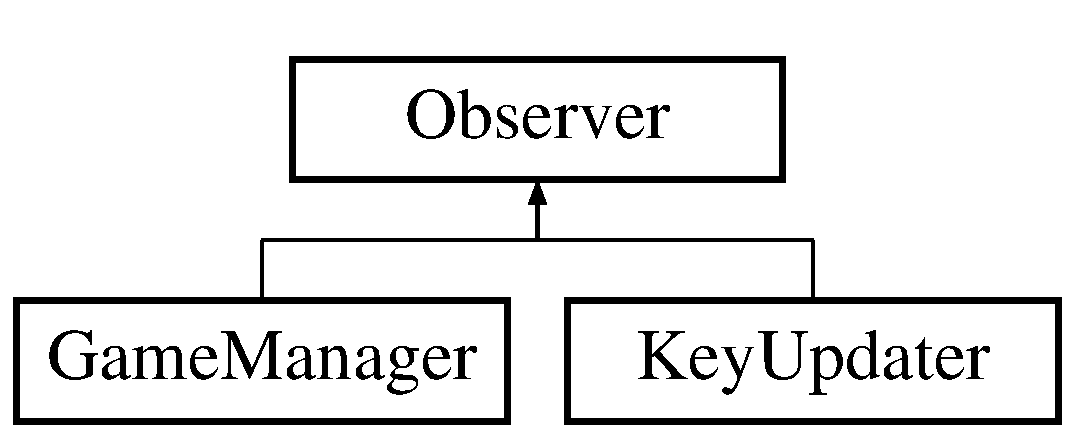
\includegraphics[height=2.000000cm]{class_observer}
\end{center}
\end{figure}
\subsection*{Public Member Functions}
\begin{DoxyCompactItemize}
\item 
\hyperlink{class_observer_a19c43f80a38a332a6f694783df3c9835}{Observer} ()
\item 
virtual void \hyperlink{class_observer_a7204fd48ae9f9c2f39ea7e165740c451}{update} (google\-::protobuf\-::\-Message $\ast$p\-Message)=0
\end{DoxyCompactItemize}


\subsection{Constructor \& Destructor Documentation}
\hypertarget{class_observer_a19c43f80a38a332a6f694783df3c9835}{\index{Observer@{Observer}!Observer@{Observer}}
\index{Observer@{Observer}!Observer@{Observer}}
\subsubsection[{Observer}]{\setlength{\rightskip}{0pt plus 5cm}Observer\-::\-Observer (
\begin{DoxyParamCaption}
{}
\end{DoxyParamCaption}
)}}\label{class_observer_a19c43f80a38a332a6f694783df3c9835}


\subsection{Member Function Documentation}
\hypertarget{class_observer_a7204fd48ae9f9c2f39ea7e165740c451}{\index{Observer@{Observer}!update@{update}}
\index{update@{update}!Observer@{Observer}}
\subsubsection[{update}]{\setlength{\rightskip}{0pt plus 5cm}virtual void Observer\-::update (
\begin{DoxyParamCaption}
\item[{google\-::protobuf\-::\-Message $\ast$}]{p\-Message}
\end{DoxyParamCaption}
)\hspace{0.3cm}{\ttfamily [pure virtual]}}}\label{class_observer_a7204fd48ae9f9c2f39ea7e165740c451}


Implemented in \hyperlink{class_game_manager_abcc7beda88f37957ab1c0711de030a45}{Game\-Manager}, and \hyperlink{class_key_updater_ae98e44fb4a0be038fd6482bfae40007e}{Key\-Updater}.



The documentation for this class was generated from the following files\-:\begin{DoxyCompactItemize}
\item 
logic/patterdesing/\hyperlink{observer_8h}{observer.\-h}\item 
logic/patterdesing/\hyperlink{observer_8cpp}{observer.\-cpp}\end{DoxyCompactItemize}

\hypertarget{class_paint_task}{\section{Paint\-Task Class Reference}
\label{class_paint_task}\index{Paint\-Task@{Paint\-Task}}
}
\subsection*{Public Member Functions}
\begin{DoxyCompactItemize}
\item 
\hypertarget{class_paint_task_a95c518e8d1f1b47513fcbb7d33efae92}{{\bfseries Paint\-Task} (Q\-Rect p\-Rec, Q\-Pixmap $\ast$p\-Pix)}\label{class_paint_task_a95c518e8d1f1b47513fcbb7d33efae92}

\item 
\hypertarget{class_paint_task_aa6a868686cea358b91056a7bdd17c39c}{{\bfseries Paint\-Task} (const \hyperlink{class_paint_task}{Paint\-Task} \&pt)}\label{class_paint_task_aa6a868686cea358b91056a7bdd17c39c}

\item 
\hypertarget{class_paint_task_a2cfc517eefcaf5190c3c138402edf24a}{Q\-Rect {\bfseries get\-Rec} () const }\label{class_paint_task_a2cfc517eefcaf5190c3c138402edf24a}

\item 
\hypertarget{class_paint_task_a589af1cb82beb781e4cc34027f73bdf0}{void {\bfseries set\-Rec} (const Q\-Rect \&value)}\label{class_paint_task_a589af1cb82beb781e4cc34027f73bdf0}

\item 
\hypertarget{class_paint_task_ad32c94ebc7a9b5640179ccbf00a0398e}{Q\-Pixmap $\ast$ {\bfseries get\-Pix} () const }\label{class_paint_task_ad32c94ebc7a9b5640179ccbf00a0398e}

\item 
\hypertarget{class_paint_task_aba6f4430d04a3202950719145f89597c}{void {\bfseries set\-Pix} (Q\-Pixmap $\ast$value)}\label{class_paint_task_aba6f4430d04a3202950719145f89597c}

\end{DoxyCompactItemize}


The documentation for this class was generated from the following files\-:\begin{DoxyCompactItemize}
\item 
painttask.\-h\item 
painttask.\-cpp\end{DoxyCompactItemize}

\hypertarget{class_pause}{\section{Pause Class Reference}
\label{class_pause}\index{Pause@{Pause}}
}
Inheritance diagram for Pause\-:\begin{figure}[H]
\begin{center}
\leavevmode
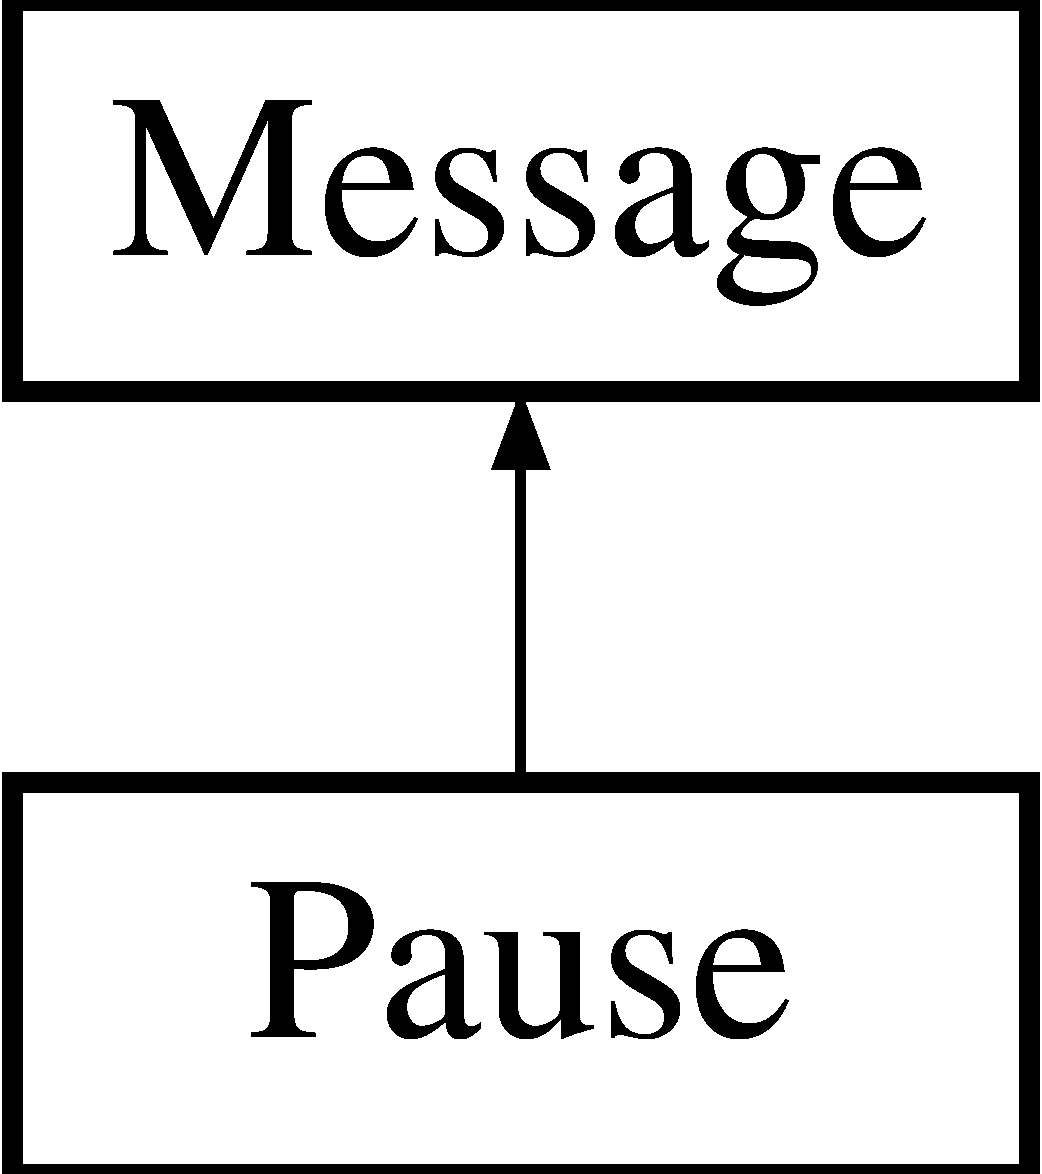
\includegraphics[height=2.000000cm]{class_pause}
\end{center}
\end{figure}
\subsection*{Public Member Functions}
\begin{DoxyCompactItemize}
\item 
\hypertarget{class_pause_a6d9f3c3c86804f1018e41981fce7a5de}{{\bfseries Pause} (const \hyperlink{class_pause}{Pause} \&from)}\label{class_pause_a6d9f3c3c86804f1018e41981fce7a5de}

\item 
\hypertarget{class_pause_a2d65a031f1dcdb67e4536b22c8ab414f}{\hyperlink{class_pause}{Pause} \& {\bfseries operator=} (const \hyperlink{class_pause}{Pause} \&from)}\label{class_pause_a2d65a031f1dcdb67e4536b22c8ab414f}

\item 
\hypertarget{class_pause_a5b5c631de45d3cd394c8e6ce35319bca}{const \\*
\-::google\-::protobuf\-::\-Unknown\-Field\-Set \& {\bfseries unknown\-\_\-fields} () const }\label{class_pause_a5b5c631de45d3cd394c8e6ce35319bca}

\item 
\hypertarget{class_pause_a7e4d5b5e01a70b9eb30e839898efcac2}{inline\-::google\-::protobuf\-::\-Unknown\-Field\-Set $\ast$ {\bfseries mutable\-\_\-unknown\-\_\-fields} ()}\label{class_pause_a7e4d5b5e01a70b9eb30e839898efcac2}

\item 
\hypertarget{class_pause_ad587734aa5f89360a446f7524e72c713}{void {\bfseries Swap} (\hyperlink{class_pause}{Pause} $\ast$other)}\label{class_pause_ad587734aa5f89360a446f7524e72c713}

\item 
\hypertarget{class_pause_ac7a15b915ffd6d9871010ea21dda6af7}{\hyperlink{class_pause}{Pause} $\ast$ {\bfseries New} () const }\label{class_pause_ac7a15b915ffd6d9871010ea21dda6af7}

\item 
\hypertarget{class_pause_abc7f5cc2e44167593126dc7e02c6a281}{\hyperlink{class_pause}{Pause} $\ast$ {\bfseries New} (\-::google\-::protobuf\-::\-Arena $\ast$arena) const }\label{class_pause_abc7f5cc2e44167593126dc7e02c6a281}

\item 
\hypertarget{class_pause_ac3b45e0a8a112543955e9dec70720c33}{void {\bfseries Copy\-From} (const \-::google\-::protobuf\-::\-Message \&from)}\label{class_pause_ac3b45e0a8a112543955e9dec70720c33}

\item 
\hypertarget{class_pause_a4d7a23a24b2199df9e8af317cd9efd52}{void {\bfseries Merge\-From} (const \-::google\-::protobuf\-::\-Message \&from)}\label{class_pause_a4d7a23a24b2199df9e8af317cd9efd52}

\item 
\hypertarget{class_pause_a8a4f7ea801fa755ad33ec4c503e8c36e}{void {\bfseries Copy\-From} (const \hyperlink{class_pause}{Pause} \&from)}\label{class_pause_a8a4f7ea801fa755ad33ec4c503e8c36e}

\item 
\hypertarget{class_pause_a0363eac7eeaeb5bee0d8be630581aa94}{void {\bfseries Merge\-From} (const \hyperlink{class_pause}{Pause} \&from)}\label{class_pause_a0363eac7eeaeb5bee0d8be630581aa94}

\item 
\hypertarget{class_pause_a17c998beccec414a6293b7e83281b3a2}{void {\bfseries Clear} ()}\label{class_pause_a17c998beccec414a6293b7e83281b3a2}

\item 
\hypertarget{class_pause_a5ac3603904cbb13f443e4a79386f3247}{bool {\bfseries Is\-Initialized} () const }\label{class_pause_a5ac3603904cbb13f443e4a79386f3247}

\item 
\hypertarget{class_pause_a4ad86c01ac23daac3e82658eca137666}{int {\bfseries Byte\-Size} () const }\label{class_pause_a4ad86c01ac23daac3e82658eca137666}

\item 
\hypertarget{class_pause_abc751f0e64bdb9043bf3a1b56c5c89f4}{bool {\bfseries Merge\-Partial\-From\-Coded\-Stream} (\-::google\-::protobuf\-::io\-::\-Coded\-Input\-Stream $\ast$input)}\label{class_pause_abc751f0e64bdb9043bf3a1b56c5c89f4}

\item 
\hypertarget{class_pause_a2fb568f1850b6cdd8eaa699cab95b56e}{void {\bfseries Serialize\-With\-Cached\-Sizes} (\-::google\-::protobuf\-::io\-::\-Coded\-Output\-Stream $\ast$output) const }\label{class_pause_a2fb568f1850b6cdd8eaa699cab95b56e}

\item 
\hypertarget{class_pause_a3b78bd2c68b91fff5589432206b5b7d1}{\-::google\-::protobuf\-::uint8 $\ast$ {\bfseries Serialize\-With\-Cached\-Sizes\-To\-Array} (\-::google\-::protobuf\-::uint8 $\ast$output) const }\label{class_pause_a3b78bd2c68b91fff5589432206b5b7d1}

\item 
\hypertarget{class_pause_a2af36b0dec18ac3b93b02208cf2c66d3}{int {\bfseries Get\-Cached\-Size} () const }\label{class_pause_a2af36b0dec18ac3b93b02208cf2c66d3}

\item 
\hypertarget{class_pause_af38c3c10a11ca18dd476c8b076a03c80}{\-::google\-::protobuf\-::\-Metadata {\bfseries Get\-Metadata} () const }\label{class_pause_af38c3c10a11ca18dd476c8b076a03c80}

\item 
\hypertarget{class_pause_afcdd5b8246226aafa60f6f639718271c}{bool {\bfseries has\-\_\-numofplayers} () const }\label{class_pause_afcdd5b8246226aafa60f6f639718271c}

\item 
\hypertarget{class_pause_a1a4311ac60f3ffcf15e10ad064df6a0f}{void {\bfseries clear\-\_\-numofplayers} ()}\label{class_pause_a1a4311ac60f3ffcf15e10ad064df6a0f}

\item 
\hypertarget{class_pause_a282ee0b2f04d64d41b1056bd5d64eea9}{inline\-::google\-::protobuf\-::int32 {\bfseries numofplayers} () const }\label{class_pause_a282ee0b2f04d64d41b1056bd5d64eea9}

\item 
\hypertarget{class_pause_ade24c4a530fb2eb508bf2f24b7a7e47f}{void {\bfseries set\-\_\-numofplayers} (\-::google\-::protobuf\-::int32 value)}\label{class_pause_ade24c4a530fb2eb508bf2f24b7a7e47f}

\end{DoxyCompactItemize}
\subsection*{Static Public Member Functions}
\begin{DoxyCompactItemize}
\item 
\hypertarget{class_pause_a25b48247864d5ce493fdf1363115076e}{static const \\*
\-::google\-::protobuf\-::\-Descriptor $\ast$ {\bfseries descriptor} ()}\label{class_pause_a25b48247864d5ce493fdf1363115076e}

\item 
\hypertarget{class_pause_a67c55d1187b0e4b77c9b74c0b8a6b5d7}{static const \hyperlink{class_pause}{Pause} \& {\bfseries default\-\_\-instance} ()}\label{class_pause_a67c55d1187b0e4b77c9b74c0b8a6b5d7}

\end{DoxyCompactItemize}
\subsection*{Static Public Attributes}
\begin{DoxyCompactItemize}
\item 
\hypertarget{class_pause_a3db8e5c058abd2047804f210d5f982ae}{static const int {\bfseries k\-Num\-Of\-Players\-Field\-Number} = 1}\label{class_pause_a3db8e5c058abd2047804f210d5f982ae}

\end{DoxyCompactItemize}
\subsection*{Friends}
\begin{DoxyCompactItemize}
\item 
\hypertarget{class_pause_a6dd83dd31565ad93783f8d042924d6f3}{void {\bfseries protobuf\-\_\-\-Add\-Desc\-\_\-\-Pause\-\_\-2eproto} ()}\label{class_pause_a6dd83dd31565ad93783f8d042924d6f3}

\item 
\hypertarget{class_pause_a53e5c86813ef675cf1916aa78bc72131}{void {\bfseries protobuf\-\_\-\-Assign\-Desc\-\_\-\-Pause\-\_\-2eproto} ()}\label{class_pause_a53e5c86813ef675cf1916aa78bc72131}

\item 
\hypertarget{class_pause_a5e08f905ac1c337aaf3fc36ffff15713}{void {\bfseries protobuf\-\_\-\-Shutdown\-File\-\_\-\-Pause\-\_\-2eproto} ()}\label{class_pause_a5e08f905ac1c337aaf3fc36ffff15713}

\end{DoxyCompactItemize}


The documentation for this class was generated from the following files\-:\begin{DoxyCompactItemize}
\item 
protobufmessage/Pause.\-pb.\-h\item 
protobufmessage/Pause.\-pb.\-cc\end{DoxyCompactItemize}

\hypertarget{class_pause_other_players}{\section{Pause\-Other\-Players Class Reference}
\label{class_pause_other_players}\index{Pause\-Other\-Players@{Pause\-Other\-Players}}
}


{\ttfamily \#include $<$Pause\-Other\-Players.\-pb.\-h$>$}

Inheritance diagram for Pause\-Other\-Players\-:\begin{figure}[H]
\begin{center}
\leavevmode
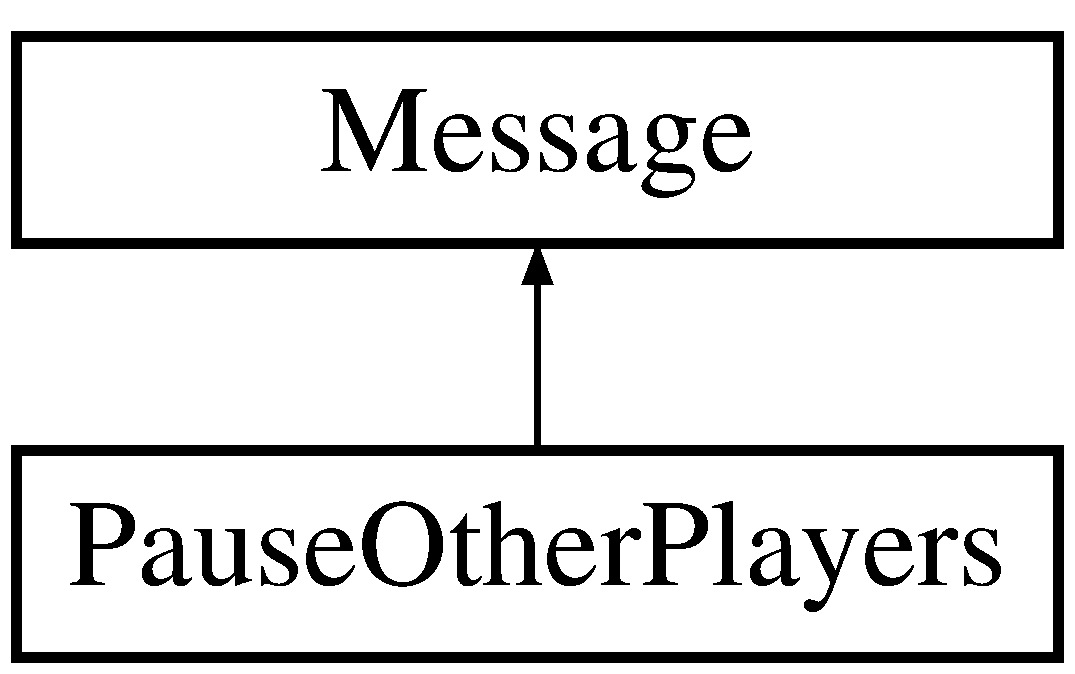
\includegraphics[height=2.000000cm]{class_pause_other_players}
\end{center}
\end{figure}
\subsection*{Public Member Functions}
\begin{DoxyCompactItemize}
\item 
\hyperlink{class_pause_other_players_a0712df06b1ecd8663b3cdaf25ed83afa}{Pause\-Other\-Players} ()
\item 
virtual \hyperlink{class_pause_other_players_a9becaa73e48de9ed2f3086e8f89b9f23}{$\sim$\-Pause\-Other\-Players} ()
\item 
\hyperlink{class_pause_other_players_a27bbeda44b6b6e905276c0a6a5f38702}{Pause\-Other\-Players} (const \hyperlink{class_pause_other_players}{Pause\-Other\-Players} \&from)
\item 
\hyperlink{class_pause_other_players}{Pause\-Other\-Players} \& \hyperlink{class_pause_other_players_aa77bc93b6bccd761f4360c56b784e1aa}{operator=} (const \hyperlink{class_pause_other_players}{Pause\-Other\-Players} \&from)
\item 
const \\*
\-::google\-::protobuf\-::\-Unknown\-Field\-Set \& \hyperlink{class_pause_other_players_a4b909a26d8345e6efbaac4a18d97cc27}{unknown\-\_\-fields} () const 
\item 
inline\-::google\-::protobuf\-::\-Unknown\-Field\-Set $\ast$ \hyperlink{class_pause_other_players_a1736e5ae730a67ca4d70a7a7fb252f09}{mutable\-\_\-unknown\-\_\-fields} ()
\item 
void \hyperlink{class_pause_other_players_a197ba9c7116c63439e83c9365ceb57e0}{Swap} (\hyperlink{class_pause_other_players}{Pause\-Other\-Players} $\ast$other)
\item 
\hyperlink{class_pause_other_players}{Pause\-Other\-Players} $\ast$ \hyperlink{class_pause_other_players_a7732cb5a8cfb74cd10d5ef5003860ee8}{New} () const 
\item 
\hyperlink{class_pause_other_players}{Pause\-Other\-Players} $\ast$ \hyperlink{class_pause_other_players_a35ff08f92a7f3996646b99ea055ca8dc}{New} (\-::google\-::protobuf\-::\-Arena $\ast$arena) const 
\item 
void \hyperlink{class_pause_other_players_adb110b8a4f8a0213d25e732180c49d42}{Copy\-From} (const \-::google\-::protobuf\-::\-Message \&from)
\item 
void \hyperlink{class_pause_other_players_ab72874774c57843b378e3c11ef49b15c}{Merge\-From} (const \-::google\-::protobuf\-::\-Message \&from)
\item 
void \hyperlink{class_pause_other_players_a39f245baeca634ba592ec1f199d87d8a}{Copy\-From} (const \hyperlink{class_pause_other_players}{Pause\-Other\-Players} \&from)
\item 
void \hyperlink{class_pause_other_players_a11a8b7c8f85f83e6173a78dda661d246}{Merge\-From} (const \hyperlink{class_pause_other_players}{Pause\-Other\-Players} \&from)
\item 
void \hyperlink{class_pause_other_players_a2533a4232c5aa13911ed738a3d7c0e0a}{Clear} ()
\item 
bool \hyperlink{class_pause_other_players_ab959487ba39f0f04be65a691486a5f09}{Is\-Initialized} () const 
\item 
int \hyperlink{class_pause_other_players_a822d5b333583bce0d014a39edeb0f933}{Byte\-Size} () const 
\item 
bool \hyperlink{class_pause_other_players_a1e0909de2b4d416c2139b3352fb5be06}{Merge\-Partial\-From\-Coded\-Stream} (\-::google\-::protobuf\-::io\-::\-Coded\-Input\-Stream $\ast$input)
\item 
void \hyperlink{class_pause_other_players_a0d11eee8c31de806930b34cc20ba4ca0}{Serialize\-With\-Cached\-Sizes} (\-::google\-::protobuf\-::io\-::\-Coded\-Output\-Stream $\ast$output) const 
\item 
\-::google\-::protobuf\-::uint8 $\ast$ \hyperlink{class_pause_other_players_a946433ba2849ab63b3f6824bbcdd0280}{Serialize\-With\-Cached\-Sizes\-To\-Array} (\-::google\-::protobuf\-::uint8 $\ast$output) const 
\item 
int \hyperlink{class_pause_other_players_ac74be5a0f00009b5a21590c2e8c83987}{Get\-Cached\-Size} () const 
\item 
\-::google\-::protobuf\-::\-Metadata \hyperlink{class_pause_other_players_afbca7aa83badf6f3c59be35869d1b75c}{Get\-Metadata} () const 
\item 
bool \hyperlink{class_pause_other_players_aafa7dd371c5b5f3810138683a93f7ed6}{has\-\_\-paused} () const 
\item 
void \hyperlink{class_pause_other_players_ac15c76196cd209d557c60f2d41f4602d}{clear\-\_\-paused} ()
\item 
bool \hyperlink{class_pause_other_players_a519e1195e02787240129e18ba893faaa}{paused} () const 
\item 
void \hyperlink{class_pause_other_players_ac6c380bdd56e7959a3d01ef49aacd0cc}{set\-\_\-paused} (bool value)
\end{DoxyCompactItemize}
\subsection*{Static Public Member Functions}
\begin{DoxyCompactItemize}
\item 
static const \\*
\-::google\-::protobuf\-::\-Descriptor $\ast$ \hyperlink{class_pause_other_players_a54176046797703d917a3f244fe65bc2b}{descriptor} ()
\item 
static const \hyperlink{class_pause_other_players}{Pause\-Other\-Players} \& \hyperlink{class_pause_other_players_aa7aee4f6cedf2aded36cbc684a4040c6}{default\-\_\-instance} ()
\end{DoxyCompactItemize}
\subsection*{Static Public Attributes}
\begin{DoxyCompactItemize}
\item 
static const int \hyperlink{class_pause_other_players_ad4f24b6f71dae8934ab680c37f72b144}{k\-Paused\-Field\-Number} = 1
\end{DoxyCompactItemize}
\subsection*{Friends}
\begin{DoxyCompactItemize}
\item 
void \hyperlink{class_pause_other_players_a007eaba79d9840bfe722146d0e1d6b37}{protobuf\-\_\-\-Add\-Desc\-\_\-\-Pause\-Other\-Players\-\_\-2eproto} ()
\item 
void \hyperlink{class_pause_other_players_aeb3f974c8db10b61825844f19af2809a}{protobuf\-\_\-\-Assign\-Desc\-\_\-\-Pause\-Other\-Players\-\_\-2eproto} ()
\item 
void \hyperlink{class_pause_other_players_a0499888e4edae1a466fbed0481ae977b}{protobuf\-\_\-\-Shutdown\-File\-\_\-\-Pause\-Other\-Players\-\_\-2eproto} ()
\end{DoxyCompactItemize}


\subsection{Constructor \& Destructor Documentation}
\hypertarget{class_pause_other_players_a0712df06b1ecd8663b3cdaf25ed83afa}{\index{Pause\-Other\-Players@{Pause\-Other\-Players}!Pause\-Other\-Players@{Pause\-Other\-Players}}
\index{Pause\-Other\-Players@{Pause\-Other\-Players}!PauseOtherPlayers@{Pause\-Other\-Players}}
\subsubsection[{Pause\-Other\-Players}]{\setlength{\rightskip}{0pt plus 5cm}Pause\-Other\-Players\-::\-Pause\-Other\-Players (
\begin{DoxyParamCaption}
{}
\end{DoxyParamCaption}
)}}\label{class_pause_other_players_a0712df06b1ecd8663b3cdaf25ed83afa}
\hypertarget{class_pause_other_players_a9becaa73e48de9ed2f3086e8f89b9f23}{\index{Pause\-Other\-Players@{Pause\-Other\-Players}!$\sim$\-Pause\-Other\-Players@{$\sim$\-Pause\-Other\-Players}}
\index{$\sim$\-Pause\-Other\-Players@{$\sim$\-Pause\-Other\-Players}!PauseOtherPlayers@{Pause\-Other\-Players}}
\subsubsection[{$\sim$\-Pause\-Other\-Players}]{\setlength{\rightskip}{0pt plus 5cm}Pause\-Other\-Players\-::$\sim$\-Pause\-Other\-Players (
\begin{DoxyParamCaption}
{}
\end{DoxyParamCaption}
)\hspace{0.3cm}{\ttfamily [virtual]}}}\label{class_pause_other_players_a9becaa73e48de9ed2f3086e8f89b9f23}
\hypertarget{class_pause_other_players_a27bbeda44b6b6e905276c0a6a5f38702}{\index{Pause\-Other\-Players@{Pause\-Other\-Players}!Pause\-Other\-Players@{Pause\-Other\-Players}}
\index{Pause\-Other\-Players@{Pause\-Other\-Players}!PauseOtherPlayers@{Pause\-Other\-Players}}
\subsubsection[{Pause\-Other\-Players}]{\setlength{\rightskip}{0pt plus 5cm}Pause\-Other\-Players\-::\-Pause\-Other\-Players (
\begin{DoxyParamCaption}
\item[{const {\bf Pause\-Other\-Players} \&}]{from}
\end{DoxyParamCaption}
)}}\label{class_pause_other_players_a27bbeda44b6b6e905276c0a6a5f38702}


\subsection{Member Function Documentation}
\hypertarget{class_pause_other_players_a822d5b333583bce0d014a39edeb0f933}{\index{Pause\-Other\-Players@{Pause\-Other\-Players}!Byte\-Size@{Byte\-Size}}
\index{Byte\-Size@{Byte\-Size}!PauseOtherPlayers@{Pause\-Other\-Players}}
\subsubsection[{Byte\-Size}]{\setlength{\rightskip}{0pt plus 5cm}int Pause\-Other\-Players\-::\-Byte\-Size (
\begin{DoxyParamCaption}
{}
\end{DoxyParamCaption}
) const}}\label{class_pause_other_players_a822d5b333583bce0d014a39edeb0f933}
\hypertarget{class_pause_other_players_a2533a4232c5aa13911ed738a3d7c0e0a}{\index{Pause\-Other\-Players@{Pause\-Other\-Players}!Clear@{Clear}}
\index{Clear@{Clear}!PauseOtherPlayers@{Pause\-Other\-Players}}
\subsubsection[{Clear}]{\setlength{\rightskip}{0pt plus 5cm}void Pause\-Other\-Players\-::\-Clear (
\begin{DoxyParamCaption}
{}
\end{DoxyParamCaption}
)}}\label{class_pause_other_players_a2533a4232c5aa13911ed738a3d7c0e0a}
\hypertarget{class_pause_other_players_ac15c76196cd209d557c60f2d41f4602d}{\index{Pause\-Other\-Players@{Pause\-Other\-Players}!clear\-\_\-paused@{clear\-\_\-paused}}
\index{clear\-\_\-paused@{clear\-\_\-paused}!PauseOtherPlayers@{Pause\-Other\-Players}}
\subsubsection[{clear\-\_\-paused}]{\setlength{\rightskip}{0pt plus 5cm}void Pause\-Other\-Players\-::clear\-\_\-paused (
\begin{DoxyParamCaption}
{}
\end{DoxyParamCaption}
)\hspace{0.3cm}{\ttfamily [inline]}}}\label{class_pause_other_players_ac15c76196cd209d557c60f2d41f4602d}
\hypertarget{class_pause_other_players_adb110b8a4f8a0213d25e732180c49d42}{\index{Pause\-Other\-Players@{Pause\-Other\-Players}!Copy\-From@{Copy\-From}}
\index{Copy\-From@{Copy\-From}!PauseOtherPlayers@{Pause\-Other\-Players}}
\subsubsection[{Copy\-From}]{\setlength{\rightskip}{0pt plus 5cm}void Pause\-Other\-Players\-::\-Copy\-From (
\begin{DoxyParamCaption}
\item[{const \-::google\-::protobuf\-::\-Message \&}]{from}
\end{DoxyParamCaption}
)}}\label{class_pause_other_players_adb110b8a4f8a0213d25e732180c49d42}
\hypertarget{class_pause_other_players_a39f245baeca634ba592ec1f199d87d8a}{\index{Pause\-Other\-Players@{Pause\-Other\-Players}!Copy\-From@{Copy\-From}}
\index{Copy\-From@{Copy\-From}!PauseOtherPlayers@{Pause\-Other\-Players}}
\subsubsection[{Copy\-From}]{\setlength{\rightskip}{0pt plus 5cm}void Pause\-Other\-Players\-::\-Copy\-From (
\begin{DoxyParamCaption}
\item[{const {\bf Pause\-Other\-Players} \&}]{from}
\end{DoxyParamCaption}
)}}\label{class_pause_other_players_a39f245baeca634ba592ec1f199d87d8a}
\hypertarget{class_pause_other_players_aa7aee4f6cedf2aded36cbc684a4040c6}{\index{Pause\-Other\-Players@{Pause\-Other\-Players}!default\-\_\-instance@{default\-\_\-instance}}
\index{default\-\_\-instance@{default\-\_\-instance}!PauseOtherPlayers@{Pause\-Other\-Players}}
\subsubsection[{default\-\_\-instance}]{\setlength{\rightskip}{0pt plus 5cm}const {\bf Pause\-Other\-Players} \& Pause\-Other\-Players\-::default\-\_\-instance (
\begin{DoxyParamCaption}
{}
\end{DoxyParamCaption}
)\hspace{0.3cm}{\ttfamily [static]}}}\label{class_pause_other_players_aa7aee4f6cedf2aded36cbc684a4040c6}
\hypertarget{class_pause_other_players_a54176046797703d917a3f244fe65bc2b}{\index{Pause\-Other\-Players@{Pause\-Other\-Players}!descriptor@{descriptor}}
\index{descriptor@{descriptor}!PauseOtherPlayers@{Pause\-Other\-Players}}
\subsubsection[{descriptor}]{\setlength{\rightskip}{0pt plus 5cm}const \-::google\-::protobuf\-::\-Descriptor $\ast$ Pause\-Other\-Players\-::descriptor (
\begin{DoxyParamCaption}
{}
\end{DoxyParamCaption}
)\hspace{0.3cm}{\ttfamily [static]}}}\label{class_pause_other_players_a54176046797703d917a3f244fe65bc2b}
\hypertarget{class_pause_other_players_ac74be5a0f00009b5a21590c2e8c83987}{\index{Pause\-Other\-Players@{Pause\-Other\-Players}!Get\-Cached\-Size@{Get\-Cached\-Size}}
\index{Get\-Cached\-Size@{Get\-Cached\-Size}!PauseOtherPlayers@{Pause\-Other\-Players}}
\subsubsection[{Get\-Cached\-Size}]{\setlength{\rightskip}{0pt plus 5cm}int Pause\-Other\-Players\-::\-Get\-Cached\-Size (
\begin{DoxyParamCaption}
{}
\end{DoxyParamCaption}
) const\hspace{0.3cm}{\ttfamily [inline]}}}\label{class_pause_other_players_ac74be5a0f00009b5a21590c2e8c83987}
\hypertarget{class_pause_other_players_afbca7aa83badf6f3c59be35869d1b75c}{\index{Pause\-Other\-Players@{Pause\-Other\-Players}!Get\-Metadata@{Get\-Metadata}}
\index{Get\-Metadata@{Get\-Metadata}!PauseOtherPlayers@{Pause\-Other\-Players}}
\subsubsection[{Get\-Metadata}]{\setlength{\rightskip}{0pt plus 5cm}google\-::protobuf\-::\-Metadata Pause\-Other\-Players\-::\-Get\-Metadata (
\begin{DoxyParamCaption}
{}
\end{DoxyParamCaption}
) const}}\label{class_pause_other_players_afbca7aa83badf6f3c59be35869d1b75c}
\hypertarget{class_pause_other_players_aafa7dd371c5b5f3810138683a93f7ed6}{\index{Pause\-Other\-Players@{Pause\-Other\-Players}!has\-\_\-paused@{has\-\_\-paused}}
\index{has\-\_\-paused@{has\-\_\-paused}!PauseOtherPlayers@{Pause\-Other\-Players}}
\subsubsection[{has\-\_\-paused}]{\setlength{\rightskip}{0pt plus 5cm}bool Pause\-Other\-Players\-::has\-\_\-paused (
\begin{DoxyParamCaption}
{}
\end{DoxyParamCaption}
) const\hspace{0.3cm}{\ttfamily [inline]}}}\label{class_pause_other_players_aafa7dd371c5b5f3810138683a93f7ed6}
\hypertarget{class_pause_other_players_ab959487ba39f0f04be65a691486a5f09}{\index{Pause\-Other\-Players@{Pause\-Other\-Players}!Is\-Initialized@{Is\-Initialized}}
\index{Is\-Initialized@{Is\-Initialized}!PauseOtherPlayers@{Pause\-Other\-Players}}
\subsubsection[{Is\-Initialized}]{\setlength{\rightskip}{0pt plus 5cm}bool Pause\-Other\-Players\-::\-Is\-Initialized (
\begin{DoxyParamCaption}
{}
\end{DoxyParamCaption}
) const}}\label{class_pause_other_players_ab959487ba39f0f04be65a691486a5f09}
\hypertarget{class_pause_other_players_ab72874774c57843b378e3c11ef49b15c}{\index{Pause\-Other\-Players@{Pause\-Other\-Players}!Merge\-From@{Merge\-From}}
\index{Merge\-From@{Merge\-From}!PauseOtherPlayers@{Pause\-Other\-Players}}
\subsubsection[{Merge\-From}]{\setlength{\rightskip}{0pt plus 5cm}void Pause\-Other\-Players\-::\-Merge\-From (
\begin{DoxyParamCaption}
\item[{const \-::google\-::protobuf\-::\-Message \&}]{from}
\end{DoxyParamCaption}
)}}\label{class_pause_other_players_ab72874774c57843b378e3c11ef49b15c}
\hypertarget{class_pause_other_players_a11a8b7c8f85f83e6173a78dda661d246}{\index{Pause\-Other\-Players@{Pause\-Other\-Players}!Merge\-From@{Merge\-From}}
\index{Merge\-From@{Merge\-From}!PauseOtherPlayers@{Pause\-Other\-Players}}
\subsubsection[{Merge\-From}]{\setlength{\rightskip}{0pt plus 5cm}void Pause\-Other\-Players\-::\-Merge\-From (
\begin{DoxyParamCaption}
\item[{const {\bf Pause\-Other\-Players} \&}]{from}
\end{DoxyParamCaption}
)}}\label{class_pause_other_players_a11a8b7c8f85f83e6173a78dda661d246}
\hypertarget{class_pause_other_players_a1e0909de2b4d416c2139b3352fb5be06}{\index{Pause\-Other\-Players@{Pause\-Other\-Players}!Merge\-Partial\-From\-Coded\-Stream@{Merge\-Partial\-From\-Coded\-Stream}}
\index{Merge\-Partial\-From\-Coded\-Stream@{Merge\-Partial\-From\-Coded\-Stream}!PauseOtherPlayers@{Pause\-Other\-Players}}
\subsubsection[{Merge\-Partial\-From\-Coded\-Stream}]{\setlength{\rightskip}{0pt plus 5cm}bool Pause\-Other\-Players\-::\-Merge\-Partial\-From\-Coded\-Stream (
\begin{DoxyParamCaption}
\item[{\-::google\-::protobuf\-::io\-::\-Coded\-Input\-Stream $\ast$}]{input}
\end{DoxyParamCaption}
)}}\label{class_pause_other_players_a1e0909de2b4d416c2139b3352fb5be06}
\hypertarget{class_pause_other_players_a1736e5ae730a67ca4d70a7a7fb252f09}{\index{Pause\-Other\-Players@{Pause\-Other\-Players}!mutable\-\_\-unknown\-\_\-fields@{mutable\-\_\-unknown\-\_\-fields}}
\index{mutable\-\_\-unknown\-\_\-fields@{mutable\-\_\-unknown\-\_\-fields}!PauseOtherPlayers@{Pause\-Other\-Players}}
\subsubsection[{mutable\-\_\-unknown\-\_\-fields}]{\setlength{\rightskip}{0pt plus 5cm}inline \-::google\-::protobuf\-::\-Unknown\-Field\-Set$\ast$ Pause\-Other\-Players\-::mutable\-\_\-unknown\-\_\-fields (
\begin{DoxyParamCaption}
{}
\end{DoxyParamCaption}
)\hspace{0.3cm}{\ttfamily [inline]}}}\label{class_pause_other_players_a1736e5ae730a67ca4d70a7a7fb252f09}
\hypertarget{class_pause_other_players_a7732cb5a8cfb74cd10d5ef5003860ee8}{\index{Pause\-Other\-Players@{Pause\-Other\-Players}!New@{New}}
\index{New@{New}!PauseOtherPlayers@{Pause\-Other\-Players}}
\subsubsection[{New}]{\setlength{\rightskip}{0pt plus 5cm}{\bf Pause\-Other\-Players}$\ast$ Pause\-Other\-Players\-::\-New (
\begin{DoxyParamCaption}
{}
\end{DoxyParamCaption}
) const\hspace{0.3cm}{\ttfamily [inline]}}}\label{class_pause_other_players_a7732cb5a8cfb74cd10d5ef5003860ee8}
\hypertarget{class_pause_other_players_a35ff08f92a7f3996646b99ea055ca8dc}{\index{Pause\-Other\-Players@{Pause\-Other\-Players}!New@{New}}
\index{New@{New}!PauseOtherPlayers@{Pause\-Other\-Players}}
\subsubsection[{New}]{\setlength{\rightskip}{0pt plus 5cm}{\bf Pause\-Other\-Players} $\ast$ Pause\-Other\-Players\-::\-New (
\begin{DoxyParamCaption}
\item[{\-::google\-::protobuf\-::\-Arena $\ast$}]{arena}
\end{DoxyParamCaption}
) const}}\label{class_pause_other_players_a35ff08f92a7f3996646b99ea055ca8dc}
\hypertarget{class_pause_other_players_aa77bc93b6bccd761f4360c56b784e1aa}{\index{Pause\-Other\-Players@{Pause\-Other\-Players}!operator=@{operator=}}
\index{operator=@{operator=}!PauseOtherPlayers@{Pause\-Other\-Players}}
\subsubsection[{operator=}]{\setlength{\rightskip}{0pt plus 5cm}{\bf Pause\-Other\-Players}\& Pause\-Other\-Players\-::operator= (
\begin{DoxyParamCaption}
\item[{const {\bf Pause\-Other\-Players} \&}]{from}
\end{DoxyParamCaption}
)\hspace{0.3cm}{\ttfamily [inline]}}}\label{class_pause_other_players_aa77bc93b6bccd761f4360c56b784e1aa}
\hypertarget{class_pause_other_players_a519e1195e02787240129e18ba893faaa}{\index{Pause\-Other\-Players@{Pause\-Other\-Players}!paused@{paused}}
\index{paused@{paused}!PauseOtherPlayers@{Pause\-Other\-Players}}
\subsubsection[{paused}]{\setlength{\rightskip}{0pt plus 5cm}bool Pause\-Other\-Players\-::paused (
\begin{DoxyParamCaption}
{}
\end{DoxyParamCaption}
) const\hspace{0.3cm}{\ttfamily [inline]}}}\label{class_pause_other_players_a519e1195e02787240129e18ba893faaa}
\hypertarget{class_pause_other_players_a0d11eee8c31de806930b34cc20ba4ca0}{\index{Pause\-Other\-Players@{Pause\-Other\-Players}!Serialize\-With\-Cached\-Sizes@{Serialize\-With\-Cached\-Sizes}}
\index{Serialize\-With\-Cached\-Sizes@{Serialize\-With\-Cached\-Sizes}!PauseOtherPlayers@{Pause\-Other\-Players}}
\subsubsection[{Serialize\-With\-Cached\-Sizes}]{\setlength{\rightskip}{0pt plus 5cm}void Pause\-Other\-Players\-::\-Serialize\-With\-Cached\-Sizes (
\begin{DoxyParamCaption}
\item[{\-::google\-::protobuf\-::io\-::\-Coded\-Output\-Stream $\ast$}]{output}
\end{DoxyParamCaption}
) const}}\label{class_pause_other_players_a0d11eee8c31de806930b34cc20ba4ca0}
\hypertarget{class_pause_other_players_a946433ba2849ab63b3f6824bbcdd0280}{\index{Pause\-Other\-Players@{Pause\-Other\-Players}!Serialize\-With\-Cached\-Sizes\-To\-Array@{Serialize\-With\-Cached\-Sizes\-To\-Array}}
\index{Serialize\-With\-Cached\-Sizes\-To\-Array@{Serialize\-With\-Cached\-Sizes\-To\-Array}!PauseOtherPlayers@{Pause\-Other\-Players}}
\subsubsection[{Serialize\-With\-Cached\-Sizes\-To\-Array}]{\setlength{\rightskip}{0pt plus 5cm}google\-::protobuf\-::uint8 $\ast$ Pause\-Other\-Players\-::\-Serialize\-With\-Cached\-Sizes\-To\-Array (
\begin{DoxyParamCaption}
\item[{\-::google\-::protobuf\-::uint8 $\ast$}]{output}
\end{DoxyParamCaption}
) const}}\label{class_pause_other_players_a946433ba2849ab63b3f6824bbcdd0280}
\hypertarget{class_pause_other_players_ac6c380bdd56e7959a3d01ef49aacd0cc}{\index{Pause\-Other\-Players@{Pause\-Other\-Players}!set\-\_\-paused@{set\-\_\-paused}}
\index{set\-\_\-paused@{set\-\_\-paused}!PauseOtherPlayers@{Pause\-Other\-Players}}
\subsubsection[{set\-\_\-paused}]{\setlength{\rightskip}{0pt plus 5cm}void Pause\-Other\-Players\-::set\-\_\-paused (
\begin{DoxyParamCaption}
\item[{bool}]{value}
\end{DoxyParamCaption}
)\hspace{0.3cm}{\ttfamily [inline]}}}\label{class_pause_other_players_ac6c380bdd56e7959a3d01ef49aacd0cc}
\hypertarget{class_pause_other_players_a197ba9c7116c63439e83c9365ceb57e0}{\index{Pause\-Other\-Players@{Pause\-Other\-Players}!Swap@{Swap}}
\index{Swap@{Swap}!PauseOtherPlayers@{Pause\-Other\-Players}}
\subsubsection[{Swap}]{\setlength{\rightskip}{0pt plus 5cm}void Pause\-Other\-Players\-::\-Swap (
\begin{DoxyParamCaption}
\item[{{\bf Pause\-Other\-Players} $\ast$}]{other}
\end{DoxyParamCaption}
)}}\label{class_pause_other_players_a197ba9c7116c63439e83c9365ceb57e0}
\hypertarget{class_pause_other_players_a4b909a26d8345e6efbaac4a18d97cc27}{\index{Pause\-Other\-Players@{Pause\-Other\-Players}!unknown\-\_\-fields@{unknown\-\_\-fields}}
\index{unknown\-\_\-fields@{unknown\-\_\-fields}!PauseOtherPlayers@{Pause\-Other\-Players}}
\subsubsection[{unknown\-\_\-fields}]{\setlength{\rightskip}{0pt plus 5cm}const \-::google\-::protobuf\-::\-Unknown\-Field\-Set\& Pause\-Other\-Players\-::unknown\-\_\-fields (
\begin{DoxyParamCaption}
{}
\end{DoxyParamCaption}
) const\hspace{0.3cm}{\ttfamily [inline]}}}\label{class_pause_other_players_a4b909a26d8345e6efbaac4a18d97cc27}


\subsection{Friends And Related Function Documentation}
\hypertarget{class_pause_other_players_a007eaba79d9840bfe722146d0e1d6b37}{\index{Pause\-Other\-Players@{Pause\-Other\-Players}!protobuf\-\_\-\-Add\-Desc\-\_\-\-Pause\-Other\-Players\-\_\-2eproto@{protobuf\-\_\-\-Add\-Desc\-\_\-\-Pause\-Other\-Players\-\_\-2eproto}}
\index{protobuf\-\_\-\-Add\-Desc\-\_\-\-Pause\-Other\-Players\-\_\-2eproto@{protobuf\-\_\-\-Add\-Desc\-\_\-\-Pause\-Other\-Players\-\_\-2eproto}!PauseOtherPlayers@{Pause\-Other\-Players}}
\subsubsection[{protobuf\-\_\-\-Add\-Desc\-\_\-\-Pause\-Other\-Players\-\_\-2eproto}]{\setlength{\rightskip}{0pt plus 5cm}void protobuf\-\_\-\-Add\-Desc\-\_\-\-Pause\-Other\-Players\-\_\-2eproto (
\begin{DoxyParamCaption}
{}
\end{DoxyParamCaption}
)\hspace{0.3cm}{\ttfamily [friend]}}}\label{class_pause_other_players_a007eaba79d9840bfe722146d0e1d6b37}
\hypertarget{class_pause_other_players_aeb3f974c8db10b61825844f19af2809a}{\index{Pause\-Other\-Players@{Pause\-Other\-Players}!protobuf\-\_\-\-Assign\-Desc\-\_\-\-Pause\-Other\-Players\-\_\-2eproto@{protobuf\-\_\-\-Assign\-Desc\-\_\-\-Pause\-Other\-Players\-\_\-2eproto}}
\index{protobuf\-\_\-\-Assign\-Desc\-\_\-\-Pause\-Other\-Players\-\_\-2eproto@{protobuf\-\_\-\-Assign\-Desc\-\_\-\-Pause\-Other\-Players\-\_\-2eproto}!PauseOtherPlayers@{Pause\-Other\-Players}}
\subsubsection[{protobuf\-\_\-\-Assign\-Desc\-\_\-\-Pause\-Other\-Players\-\_\-2eproto}]{\setlength{\rightskip}{0pt plus 5cm}void protobuf\-\_\-\-Assign\-Desc\-\_\-\-Pause\-Other\-Players\-\_\-2eproto (
\begin{DoxyParamCaption}
{}
\end{DoxyParamCaption}
)\hspace{0.3cm}{\ttfamily [friend]}}}\label{class_pause_other_players_aeb3f974c8db10b61825844f19af2809a}
\hypertarget{class_pause_other_players_a0499888e4edae1a466fbed0481ae977b}{\index{Pause\-Other\-Players@{Pause\-Other\-Players}!protobuf\-\_\-\-Shutdown\-File\-\_\-\-Pause\-Other\-Players\-\_\-2eproto@{protobuf\-\_\-\-Shutdown\-File\-\_\-\-Pause\-Other\-Players\-\_\-2eproto}}
\index{protobuf\-\_\-\-Shutdown\-File\-\_\-\-Pause\-Other\-Players\-\_\-2eproto@{protobuf\-\_\-\-Shutdown\-File\-\_\-\-Pause\-Other\-Players\-\_\-2eproto}!PauseOtherPlayers@{Pause\-Other\-Players}}
\subsubsection[{protobuf\-\_\-\-Shutdown\-File\-\_\-\-Pause\-Other\-Players\-\_\-2eproto}]{\setlength{\rightskip}{0pt plus 5cm}void protobuf\-\_\-\-Shutdown\-File\-\_\-\-Pause\-Other\-Players\-\_\-2eproto (
\begin{DoxyParamCaption}
{}
\end{DoxyParamCaption}
)\hspace{0.3cm}{\ttfamily [friend]}}}\label{class_pause_other_players_a0499888e4edae1a466fbed0481ae977b}


\subsection{Member Data Documentation}
\hypertarget{class_pause_other_players_ad4f24b6f71dae8934ab680c37f72b144}{\index{Pause\-Other\-Players@{Pause\-Other\-Players}!k\-Paused\-Field\-Number@{k\-Paused\-Field\-Number}}
\index{k\-Paused\-Field\-Number@{k\-Paused\-Field\-Number}!PauseOtherPlayers@{Pause\-Other\-Players}}
\subsubsection[{k\-Paused\-Field\-Number}]{\setlength{\rightskip}{0pt plus 5cm}const int Pause\-Other\-Players\-::k\-Paused\-Field\-Number = 1\hspace{0.3cm}{\ttfamily [static]}}}\label{class_pause_other_players_ad4f24b6f71dae8934ab680c37f72b144}


The documentation for this class was generated from the following files\-:\begin{DoxyCompactItemize}
\item 
protobufmessage/\hyperlink{_pause_other_players_8pb_8h}{Pause\-Other\-Players.\-pb.\-h}\item 
protobufmessage/\hyperlink{_pause_other_players_8pb_8cc}{Pause\-Other\-Players.\-pb.\-cc}\end{DoxyCompactItemize}

\hypertarget{class_player}{\section{Player Class Reference}
\label{class_player}\index{Player@{Player}}
}
\subsection*{Public Member Functions}
\begin{DoxyCompactItemize}
\item 
\hypertarget{class_player_a24659ea97da1acc913319776705aab94}{{\bfseries Player} (int p\-X, int p\-Y, int p\-Player\-Number)}\label{class_player_a24659ea97da1acc913319776705aab94}

\item 
\hypertarget{class_player_ad2d305f9af724e761a491b7a85a020e0}{{\bfseries Player} (\hyperlink{class_player}{Player} \&)}\label{class_player_ad2d305f9af724e761a491b7a85a020e0}

\item 
\hypertarget{class_player_ae994ea7007d6da03e2b07941ec57d487}{\hyperlink{class_player_rocket}{Player\-Rocket} $\ast$ {\bfseries get\-Rocket} ()}\label{class_player_ae994ea7007d6da03e2b07941ec57d487}

\item 
\hypertarget{class_player_a609d8bc41b5975dc84419ebf8499af78}{void {\bfseries add\-Points} (int p\-Points)}\label{class_player_a609d8bc41b5975dc84419ebf8499af78}

\item 
\hypertarget{class_player_ab98ee3c0e10f7b2b65ad43b2a2929445}{int {\bfseries get\-Points} ()}\label{class_player_ab98ee3c0e10f7b2b65ad43b2a2929445}

\item 
\hypertarget{class_player_ad6220515daeec578e4edcebb0b304df4}{int {\bfseries get\-Player\-Number} () const }\label{class_player_ad6220515daeec578e4edcebb0b304df4}

\item 
\hypertarget{class_player_a2c86a52ca55e44e2de9115e0c736a155}{void {\bfseries change\-Munition} ()}\label{class_player_a2c86a52ca55e44e2de9115e0c736a155}

\item 
\hypertarget{class_player_ac0b88c415cb264d54c227dd4ef82a7d1}{bool {\bfseries is\-Dead} ()}\label{class_player_ac0b88c415cb264d54c227dd4ef82a7d1}

\item 
\hypertarget{class_player_a0a1f2222ab92d321474bd52147a2b1df}{bool {\bfseries revive} ()}\label{class_player_a0a1f2222ab92d321474bd52147a2b1df}

\item 
\hypertarget{class_player_a4cdc67fd9ca2de09af89d9ae19efe5f8}{void {\bfseries shoot} ()}\label{class_player_a4cdc67fd9ca2de09af89d9ae19efe5f8}

\item 
\hypertarget{class_player_ae02c3ddb3bff99fd2375c552e51b8560}{void {\bfseries set\-Stun\-Time} (int p\-Stun\-Time)}\label{class_player_ae02c3ddb3bff99fd2375c552e51b8560}

\item 
\hypertarget{class_player_a4f5d43c9f4394429fef4106715529ed7}{void {\bfseries delete\-Shot} (string p\-Id)}\label{class_player_a4f5d43c9f4394429fef4106715529ed7}

\item 
\hypertarget{class_player_a7a3afa150767d2c07968dc6d04b145b8}{bool {\bfseries operator$<$} (\hyperlink{class_player}{Player} const \&other\-Player)}\label{class_player_a7a3afa150767d2c07968dc6d04b145b8}

\item 
\hypertarget{class_player_aee44ed3cca127251cf0f65102c89dd8f}{bool {\bfseries operator$>$} (\hyperlink{class_player}{Player} const \&other\-Player)}\label{class_player_aee44ed3cca127251cf0f65102c89dd8f}

\item 
\hypertarget{class_player_a78258f14f551447cb997c91ada49ade6}{bool {\bfseries operator!=} (\hyperlink{class_player}{Player} const \&other\-Player)}\label{class_player_a78258f14f551447cb997c91ada49ade6}

\item 
\hypertarget{class_player_a3221fef8a645a3d9b40eb2e3594b3f60}{bool {\bfseries operator==} (\hyperlink{class_player}{Player} const \&other\-Player)}\label{class_player_a3221fef8a645a3d9b40eb2e3594b3f60}

\item 
\hypertarget{class_player_a324a27f8b07cc82afe1c4cb67906a964}{void {\bfseries update} (Q\-Rect rec)}\label{class_player_a324a27f8b07cc82afe1c4cb67906a964}

\item 
virtual \hyperlink{class_player_a749d2c00e1fe0f5c2746f7505a58c062}{$\sim$\-Player} ()
\item 
\hypertarget{class_player_ab221ec831c2a110ae5b631c782b6dbe7}{\hyperlink{class_list}{List}$<$ \hyperlink{class_shot}{Shot} $\ast$ $>$ $\ast$ {\bfseries get\-Player\-Shots} ()}\label{class_player_ab221ec831c2a110ae5b631c782b6dbe7}

\end{DoxyCompactItemize}


\subsection{Constructor \& Destructor Documentation}
\hypertarget{class_player_a749d2c00e1fe0f5c2746f7505a58c062}{\index{Player@{Player}!$\sim$\-Player@{$\sim$\-Player}}
\index{$\sim$\-Player@{$\sim$\-Player}!Player@{Player}}
\subsubsection[{$\sim$\-Player}]{\setlength{\rightskip}{0pt plus 5cm}Player\-::$\sim$\-Player (
\begin{DoxyParamCaption}
{}
\end{DoxyParamCaption}
)\hspace{0.3cm}{\ttfamily [virtual]}}}\label{class_player_a749d2c00e1fe0f5c2746f7505a58c062}
bool Player\-::operator !=(\-Player const \&to\-Compare)\{ return get\-Player\-Number() $>$ to\-Compare.\-get\-Player\-Number(); \} 

The documentation for this class was generated from the following files\-:\begin{DoxyCompactItemize}
\item 
logic/player.\-h\item 
logic/player.\-cpp\end{DoxyCompactItemize}

\hypertarget{class_player_is_created}{\section{Player\-Is\-Created Class Reference}
\label{class_player_is_created}\index{Player\-Is\-Created@{Player\-Is\-Created}}
}
Inheritance diagram for Player\-Is\-Created\-:\begin{figure}[H]
\begin{center}
\leavevmode
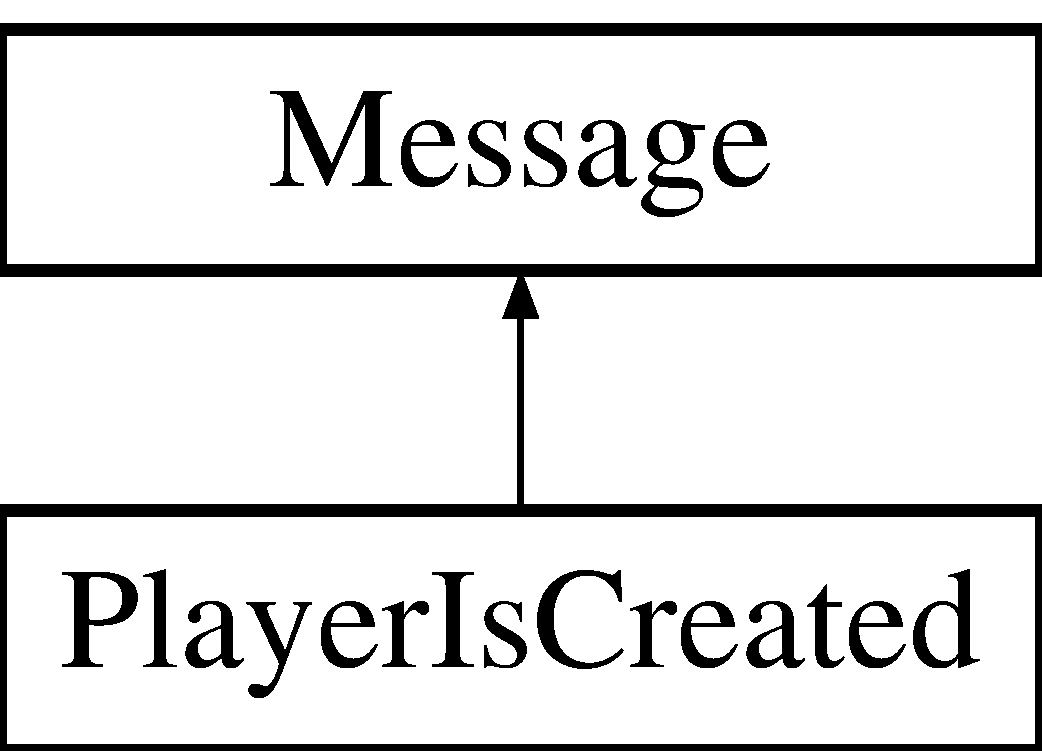
\includegraphics[height=2.000000cm]{class_player_is_created}
\end{center}
\end{figure}
\subsection*{Public Member Functions}
\begin{DoxyCompactItemize}
\item 
\hypertarget{class_player_is_created_ae905e532042d12b2c289b3affb8dd903}{{\bfseries Player\-Is\-Created} (const \hyperlink{class_player_is_created}{Player\-Is\-Created} \&from)}\label{class_player_is_created_ae905e532042d12b2c289b3affb8dd903}

\item 
\hypertarget{class_player_is_created_aef6d923f253b5eb33ac0623f73290e4e}{\hyperlink{class_player_is_created}{Player\-Is\-Created} \& {\bfseries operator=} (const \hyperlink{class_player_is_created}{Player\-Is\-Created} \&from)}\label{class_player_is_created_aef6d923f253b5eb33ac0623f73290e4e}

\item 
\hypertarget{class_player_is_created_afee68e43e7b6d43a14cbe716d304d506}{const \\*
\-::google\-::protobuf\-::\-Unknown\-Field\-Set \& {\bfseries unknown\-\_\-fields} () const }\label{class_player_is_created_afee68e43e7b6d43a14cbe716d304d506}

\item 
\hypertarget{class_player_is_created_a04590b849c6fb6b6f3fdde289e6c8d3c}{inline\-::google\-::protobuf\-::\-Unknown\-Field\-Set $\ast$ {\bfseries mutable\-\_\-unknown\-\_\-fields} ()}\label{class_player_is_created_a04590b849c6fb6b6f3fdde289e6c8d3c}

\item 
\hypertarget{class_player_is_created_a63a11c81586cf8e47746156ccae99730}{void {\bfseries Swap} (\hyperlink{class_player_is_created}{Player\-Is\-Created} $\ast$other)}\label{class_player_is_created_a63a11c81586cf8e47746156ccae99730}

\item 
\hypertarget{class_player_is_created_a52f0592fe68576e9cd73e2c892d514ac}{\hyperlink{class_player_is_created}{Player\-Is\-Created} $\ast$ {\bfseries New} () const }\label{class_player_is_created_a52f0592fe68576e9cd73e2c892d514ac}

\item 
\hypertarget{class_player_is_created_a224bc1932f4a20ea62cc4bd0107d270f}{\hyperlink{class_player_is_created}{Player\-Is\-Created} $\ast$ {\bfseries New} (\-::google\-::protobuf\-::\-Arena $\ast$arena) const }\label{class_player_is_created_a224bc1932f4a20ea62cc4bd0107d270f}

\item 
\hypertarget{class_player_is_created_a5c404f5ee81f48971becae826bd7afec}{void {\bfseries Copy\-From} (const \-::google\-::protobuf\-::\-Message \&from)}\label{class_player_is_created_a5c404f5ee81f48971becae826bd7afec}

\item 
\hypertarget{class_player_is_created_ac6b4f0e6f5c1f465c5dbd4972cf168e3}{void {\bfseries Merge\-From} (const \-::google\-::protobuf\-::\-Message \&from)}\label{class_player_is_created_ac6b4f0e6f5c1f465c5dbd4972cf168e3}

\item 
\hypertarget{class_player_is_created_ab43a5a54241664baf89386f9d0c1a220}{void {\bfseries Copy\-From} (const \hyperlink{class_player_is_created}{Player\-Is\-Created} \&from)}\label{class_player_is_created_ab43a5a54241664baf89386f9d0c1a220}

\item 
\hypertarget{class_player_is_created_a341ddc4fd72b3d6046ba324a4a4ae87a}{void {\bfseries Merge\-From} (const \hyperlink{class_player_is_created}{Player\-Is\-Created} \&from)}\label{class_player_is_created_a341ddc4fd72b3d6046ba324a4a4ae87a}

\item 
\hypertarget{class_player_is_created_a42ba62c53797a0400873a181f706f014}{void {\bfseries Clear} ()}\label{class_player_is_created_a42ba62c53797a0400873a181f706f014}

\item 
\hypertarget{class_player_is_created_a3f8c85e6394c9681d6bc8550674b12a9}{bool {\bfseries Is\-Initialized} () const }\label{class_player_is_created_a3f8c85e6394c9681d6bc8550674b12a9}

\item 
\hypertarget{class_player_is_created_ac39384c2cda7d7478e5e237827995f1f}{int {\bfseries Byte\-Size} () const }\label{class_player_is_created_ac39384c2cda7d7478e5e237827995f1f}

\item 
\hypertarget{class_player_is_created_af968fcaea9bafaef6d27d1520ecb17df}{bool {\bfseries Merge\-Partial\-From\-Coded\-Stream} (\-::google\-::protobuf\-::io\-::\-Coded\-Input\-Stream $\ast$input)}\label{class_player_is_created_af968fcaea9bafaef6d27d1520ecb17df}

\item 
\hypertarget{class_player_is_created_aeedb3484a217702a0876097852c8fea8}{void {\bfseries Serialize\-With\-Cached\-Sizes} (\-::google\-::protobuf\-::io\-::\-Coded\-Output\-Stream $\ast$output) const }\label{class_player_is_created_aeedb3484a217702a0876097852c8fea8}

\item 
\hypertarget{class_player_is_created_a13b3f9d7a0b84e04ce730fcf54ba6603}{\-::google\-::protobuf\-::uint8 $\ast$ {\bfseries Serialize\-With\-Cached\-Sizes\-To\-Array} (\-::google\-::protobuf\-::uint8 $\ast$output) const }\label{class_player_is_created_a13b3f9d7a0b84e04ce730fcf54ba6603}

\item 
\hypertarget{class_player_is_created_a6d8061fd2cb9f20a7da3496871a54bf1}{int {\bfseries Get\-Cached\-Size} () const }\label{class_player_is_created_a6d8061fd2cb9f20a7da3496871a54bf1}

\item 
\hypertarget{class_player_is_created_adbfbc228667ab0a18842e0957557a35e}{\-::google\-::protobuf\-::\-Metadata {\bfseries Get\-Metadata} () const }\label{class_player_is_created_adbfbc228667ab0a18842e0957557a35e}

\item 
\hypertarget{class_player_is_created_ae6153984b0901ab6cd1ddce575fc4d46}{bool {\bfseries has\-\_\-player} () const }\label{class_player_is_created_ae6153984b0901ab6cd1ddce575fc4d46}

\item 
\hypertarget{class_player_is_created_a519e740c8a32d1d12a055656b343cbe2}{void {\bfseries clear\-\_\-player} ()}\label{class_player_is_created_a519e740c8a32d1d12a055656b343cbe2}

\item 
\hypertarget{class_player_is_created_af2c5f8ac5a26a1ee7a0188db7e40353c}{bool {\bfseries player} () const }\label{class_player_is_created_af2c5f8ac5a26a1ee7a0188db7e40353c}

\item 
\hypertarget{class_player_is_created_a733f2e902a0ceba19444f5674cc43298}{void {\bfseries set\-\_\-player} (bool value)}\label{class_player_is_created_a733f2e902a0ceba19444f5674cc43298}

\end{DoxyCompactItemize}
\subsection*{Static Public Member Functions}
\begin{DoxyCompactItemize}
\item 
\hypertarget{class_player_is_created_a1593f54d4c123114c10177b7cac778d0}{static const \\*
\-::google\-::protobuf\-::\-Descriptor $\ast$ {\bfseries descriptor} ()}\label{class_player_is_created_a1593f54d4c123114c10177b7cac778d0}

\item 
\hypertarget{class_player_is_created_ad4a6beb4d9c38cad9a89e77dd81e1f75}{static const \hyperlink{class_player_is_created}{Player\-Is\-Created} \& {\bfseries default\-\_\-instance} ()}\label{class_player_is_created_ad4a6beb4d9c38cad9a89e77dd81e1f75}

\end{DoxyCompactItemize}
\subsection*{Static Public Attributes}
\begin{DoxyCompactItemize}
\item 
\hypertarget{class_player_is_created_a3269ef8e31ed0329f9f23b97d8cf10c2}{static const int {\bfseries k\-Player\-Field\-Number} = 1}\label{class_player_is_created_a3269ef8e31ed0329f9f23b97d8cf10c2}

\end{DoxyCompactItemize}
\subsection*{Friends}
\begin{DoxyCompactItemize}
\item 
\hypertarget{class_player_is_created_ae862a255429cc902c40be8c48190da6d}{void {\bfseries protobuf\-\_\-\-Add\-Desc\-\_\-\-Player\-Is\-Created\-\_\-2eproto} ()}\label{class_player_is_created_ae862a255429cc902c40be8c48190da6d}

\item 
\hypertarget{class_player_is_created_af53655c5ff0c55c3693040c9e8b18236}{void {\bfseries protobuf\-\_\-\-Assign\-Desc\-\_\-\-Player\-Is\-Created\-\_\-2eproto} ()}\label{class_player_is_created_af53655c5ff0c55c3693040c9e8b18236}

\item 
\hypertarget{class_player_is_created_a99057acd602b2ff282b248946616369b}{void {\bfseries protobuf\-\_\-\-Shutdown\-File\-\_\-\-Player\-Is\-Created\-\_\-2eproto} ()}\label{class_player_is_created_a99057acd602b2ff282b248946616369b}

\end{DoxyCompactItemize}


The documentation for this class was generated from the following files\-:\begin{DoxyCompactItemize}
\item 
protobufmessage/Player\-Is\-Created.\-pb.\-h\item 
protobufmessage/Player\-Is\-Created.\-pb.\-cc\end{DoxyCompactItemize}

\hypertarget{class_player_rocket}{\section{Player\-Rocket Class Reference}
\label{class_player_rocket}\index{Player\-Rocket@{Player\-Rocket}}
}


{\ttfamily \#include $<$playerrocket.\-h$>$}

Inheritance diagram for Player\-Rocket\-:\begin{figure}[H]
\begin{center}
\leavevmode
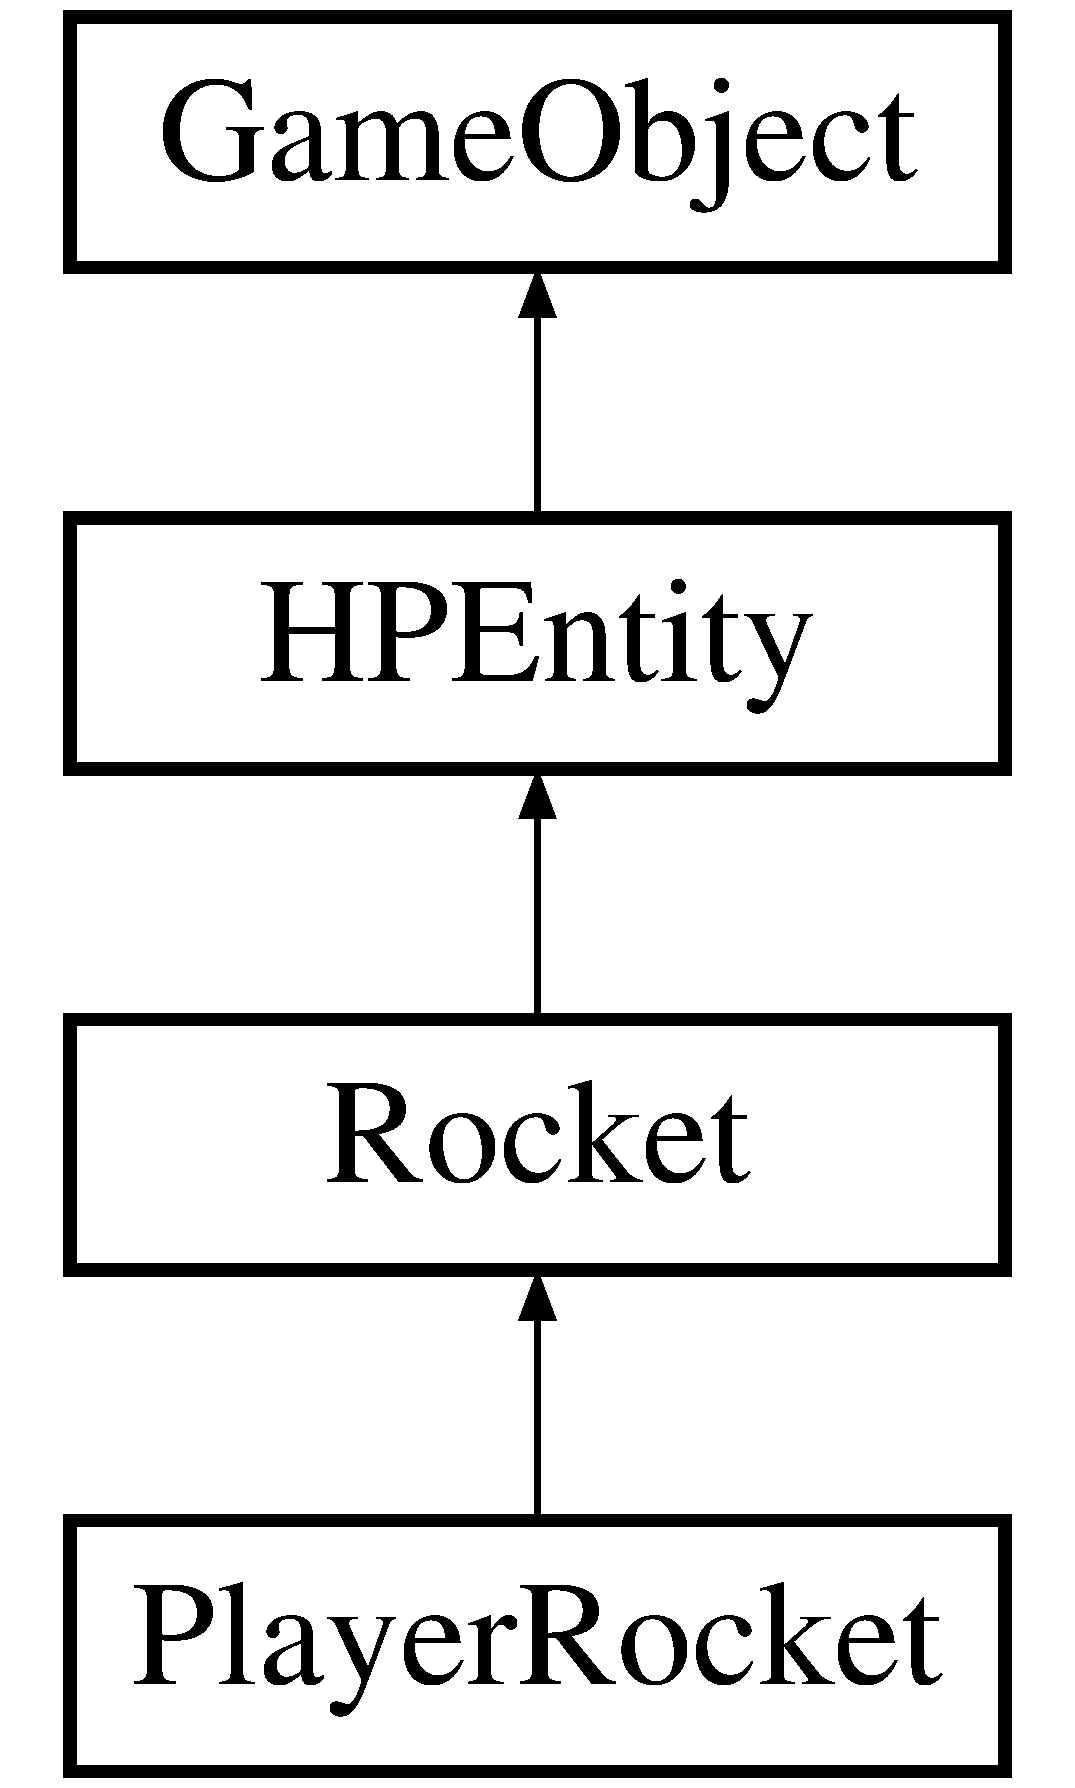
\includegraphics[height=4.000000cm]{class_player_rocket}
\end{center}
\end{figure}
\subsection*{Public Member Functions}
\begin{DoxyCompactItemize}
\item 
\hyperlink{class_player_rocket_a662448cb29201a9155de519f4563fac3}{Player\-Rocket} (Q\-Rect p\-Rectangle, int p\-Max\-Hp)
\item 
void \hyperlink{class_player_rocket_a61a775b8b7f8bf920e748eaf44af1a49}{next\-Munition} ()
\item 
void \hyperlink{class_player_rocket_a93f9d838d9b21c11ab9a2fe0176f9ff6}{add\-Munition} (int p\-Munition)
\item 
void \hyperlink{class_player_rocket_ae7bf457ff4f9c794f9cf9f8cfadf4104}{add\-Combustible} (int p\-Combustuble)
\item 
int \hyperlink{class_player_rocket_a0761ec562eed1e41ea87bff255b73090}{get\-Combustible} ()
\item 
int \hyperlink{class_player_rocket_a1c7d7b49f3ba84be78aae03201ad338c}{get\-Munitions} ()
\item 
int \hyperlink{class_player_rocket_ab9f347b5080e6db3e20f79030f50f3d8}{get\-Munition\-Type} ()
\item 
void \hyperlink{class_player_rocket_a158f4ff0dd89fd4075688fa2b7d9e693}{update} ()
\begin{DoxyCompactList}\small\item\em Actualiza el objeto, es un metodo abstracto, y debe ser implementado por sus clases hijas. \end{DoxyCompactList}\item 
\hyperlink{class_shot}{Shot} $\ast$ \hyperlink{class_player_rocket_a1277f01884b2b1a68e312228e916805a}{shoot} ()
\item 
virtual \hyperlink{class_player_rocket_aa081b938fd194297b94042efa8364c23}{$\sim$\-Player\-Rocket} ()
\end{DoxyCompactItemize}
\subsection*{Static Public Attributes}
\begin{DoxyCompactItemize}
\item 
static const int \hyperlink{class_player_rocket_a6f6bd540c91552c079a394e34d25f2c8}{C\-O\-M\-B\-U\-S\-T\-I\-B\-L\-E} = 100
\item 
static const int \hyperlink{class_player_rocket_aa3f048b7f984ee944f8daeb35cc748c2}{S\-L\-E\-E\-P\-\_\-\-T\-I\-M\-E\-\_\-\-T\-O\-\_\-\-D\-E\-C\-R\-E\-A\-S\-E\-\_\-\-C\-O\-M\-B\-U\-S\-T\-I\-B\-L\-E} = 24
\end{DoxyCompactItemize}
\subsection*{Additional Inherited Members}


\subsection{Constructor \& Destructor Documentation}
\hypertarget{class_player_rocket_a662448cb29201a9155de519f4563fac3}{\index{Player\-Rocket@{Player\-Rocket}!Player\-Rocket@{Player\-Rocket}}
\index{Player\-Rocket@{Player\-Rocket}!PlayerRocket@{Player\-Rocket}}
\subsubsection[{Player\-Rocket}]{\setlength{\rightskip}{0pt plus 5cm}Player\-Rocket\-::\-Player\-Rocket (
\begin{DoxyParamCaption}
\item[{Q\-Rect}]{p\-Rectangle, }
\item[{int}]{p\-Max\-Hp}
\end{DoxyParamCaption}
)}}\label{class_player_rocket_a662448cb29201a9155de519f4563fac3}
\hypertarget{class_player_rocket_aa081b938fd194297b94042efa8364c23}{\index{Player\-Rocket@{Player\-Rocket}!$\sim$\-Player\-Rocket@{$\sim$\-Player\-Rocket}}
\index{$\sim$\-Player\-Rocket@{$\sim$\-Player\-Rocket}!PlayerRocket@{Player\-Rocket}}
\subsubsection[{$\sim$\-Player\-Rocket}]{\setlength{\rightskip}{0pt plus 5cm}Player\-Rocket\-::$\sim$\-Player\-Rocket (
\begin{DoxyParamCaption}
{}
\end{DoxyParamCaption}
)\hspace{0.3cm}{\ttfamily [virtual]}}}\label{class_player_rocket_aa081b938fd194297b94042efa8364c23}


\subsection{Member Function Documentation}
\hypertarget{class_player_rocket_ae7bf457ff4f9c794f9cf9f8cfadf4104}{\index{Player\-Rocket@{Player\-Rocket}!add\-Combustible@{add\-Combustible}}
\index{add\-Combustible@{add\-Combustible}!PlayerRocket@{Player\-Rocket}}
\subsubsection[{add\-Combustible}]{\setlength{\rightskip}{0pt plus 5cm}void Player\-Rocket\-::add\-Combustible (
\begin{DoxyParamCaption}
\item[{int}]{p\-Combustuble}
\end{DoxyParamCaption}
)}}\label{class_player_rocket_ae7bf457ff4f9c794f9cf9f8cfadf4104}
\hypertarget{class_player_rocket_a93f9d838d9b21c11ab9a2fe0176f9ff6}{\index{Player\-Rocket@{Player\-Rocket}!add\-Munition@{add\-Munition}}
\index{add\-Munition@{add\-Munition}!PlayerRocket@{Player\-Rocket}}
\subsubsection[{add\-Munition}]{\setlength{\rightskip}{0pt plus 5cm}void Player\-Rocket\-::add\-Munition (
\begin{DoxyParamCaption}
\item[{int}]{p\-Munition}
\end{DoxyParamCaption}
)}}\label{class_player_rocket_a93f9d838d9b21c11ab9a2fe0176f9ff6}
\hypertarget{class_player_rocket_a0761ec562eed1e41ea87bff255b73090}{\index{Player\-Rocket@{Player\-Rocket}!get\-Combustible@{get\-Combustible}}
\index{get\-Combustible@{get\-Combustible}!PlayerRocket@{Player\-Rocket}}
\subsubsection[{get\-Combustible}]{\setlength{\rightskip}{0pt plus 5cm}int Player\-Rocket\-::get\-Combustible (
\begin{DoxyParamCaption}
{}
\end{DoxyParamCaption}
)}}\label{class_player_rocket_a0761ec562eed1e41ea87bff255b73090}
\hypertarget{class_player_rocket_a1c7d7b49f3ba84be78aae03201ad338c}{\index{Player\-Rocket@{Player\-Rocket}!get\-Munitions@{get\-Munitions}}
\index{get\-Munitions@{get\-Munitions}!PlayerRocket@{Player\-Rocket}}
\subsubsection[{get\-Munitions}]{\setlength{\rightskip}{0pt plus 5cm}int Player\-Rocket\-::get\-Munitions (
\begin{DoxyParamCaption}
{}
\end{DoxyParamCaption}
)}}\label{class_player_rocket_a1c7d7b49f3ba84be78aae03201ad338c}
\hypertarget{class_player_rocket_ab9f347b5080e6db3e20f79030f50f3d8}{\index{Player\-Rocket@{Player\-Rocket}!get\-Munition\-Type@{get\-Munition\-Type}}
\index{get\-Munition\-Type@{get\-Munition\-Type}!PlayerRocket@{Player\-Rocket}}
\subsubsection[{get\-Munition\-Type}]{\setlength{\rightskip}{0pt plus 5cm}int Player\-Rocket\-::get\-Munition\-Type (
\begin{DoxyParamCaption}
{}
\end{DoxyParamCaption}
)}}\label{class_player_rocket_ab9f347b5080e6db3e20f79030f50f3d8}
\hypertarget{class_player_rocket_a61a775b8b7f8bf920e748eaf44af1a49}{\index{Player\-Rocket@{Player\-Rocket}!next\-Munition@{next\-Munition}}
\index{next\-Munition@{next\-Munition}!PlayerRocket@{Player\-Rocket}}
\subsubsection[{next\-Munition}]{\setlength{\rightskip}{0pt plus 5cm}void Player\-Rocket\-::next\-Munition (
\begin{DoxyParamCaption}
{}
\end{DoxyParamCaption}
)}}\label{class_player_rocket_a61a775b8b7f8bf920e748eaf44af1a49}
\hypertarget{class_player_rocket_a1277f01884b2b1a68e312228e916805a}{\index{Player\-Rocket@{Player\-Rocket}!shoot@{shoot}}
\index{shoot@{shoot}!PlayerRocket@{Player\-Rocket}}
\subsubsection[{shoot}]{\setlength{\rightskip}{0pt plus 5cm}{\bf Shot} $\ast$ Player\-Rocket\-::shoot (
\begin{DoxyParamCaption}
{}
\end{DoxyParamCaption}
)\hspace{0.3cm}{\ttfamily [virtual]}}}\label{class_player_rocket_a1277f01884b2b1a68e312228e916805a}


Implements \hyperlink{class_rocket_a5164f5926f96291b57da2516d46262e8}{Rocket}.

\hypertarget{class_player_rocket_a158f4ff0dd89fd4075688fa2b7d9e693}{\index{Player\-Rocket@{Player\-Rocket}!update@{update}}
\index{update@{update}!PlayerRocket@{Player\-Rocket}}
\subsubsection[{update}]{\setlength{\rightskip}{0pt plus 5cm}void Player\-Rocket\-::update (
\begin{DoxyParamCaption}
{}
\end{DoxyParamCaption}
)\hspace{0.3cm}{\ttfamily [virtual]}}}\label{class_player_rocket_a158f4ff0dd89fd4075688fa2b7d9e693}


Actualiza el objeto, es un metodo abstracto, y debe ser implementado por sus clases hijas. 



Implements \hyperlink{class_game_object_ae83128d0e0efef691417779605ee037c}{Game\-Object}.



\subsection{Member Data Documentation}
\hypertarget{class_player_rocket_a6f6bd540c91552c079a394e34d25f2c8}{\index{Player\-Rocket@{Player\-Rocket}!C\-O\-M\-B\-U\-S\-T\-I\-B\-L\-E@{C\-O\-M\-B\-U\-S\-T\-I\-B\-L\-E}}
\index{C\-O\-M\-B\-U\-S\-T\-I\-B\-L\-E@{C\-O\-M\-B\-U\-S\-T\-I\-B\-L\-E}!PlayerRocket@{Player\-Rocket}}
\subsubsection[{C\-O\-M\-B\-U\-S\-T\-I\-B\-L\-E}]{\setlength{\rightskip}{0pt plus 5cm}const int Player\-Rocket\-::\-C\-O\-M\-B\-U\-S\-T\-I\-B\-L\-E = 100\hspace{0.3cm}{\ttfamily [static]}}}\label{class_player_rocket_a6f6bd540c91552c079a394e34d25f2c8}
\hypertarget{class_player_rocket_aa3f048b7f984ee944f8daeb35cc748c2}{\index{Player\-Rocket@{Player\-Rocket}!S\-L\-E\-E\-P\-\_\-\-T\-I\-M\-E\-\_\-\-T\-O\-\_\-\-D\-E\-C\-R\-E\-A\-S\-E\-\_\-\-C\-O\-M\-B\-U\-S\-T\-I\-B\-L\-E@{S\-L\-E\-E\-P\-\_\-\-T\-I\-M\-E\-\_\-\-T\-O\-\_\-\-D\-E\-C\-R\-E\-A\-S\-E\-\_\-\-C\-O\-M\-B\-U\-S\-T\-I\-B\-L\-E}}
\index{S\-L\-E\-E\-P\-\_\-\-T\-I\-M\-E\-\_\-\-T\-O\-\_\-\-D\-E\-C\-R\-E\-A\-S\-E\-\_\-\-C\-O\-M\-B\-U\-S\-T\-I\-B\-L\-E@{S\-L\-E\-E\-P\-\_\-\-T\-I\-M\-E\-\_\-\-T\-O\-\_\-\-D\-E\-C\-R\-E\-A\-S\-E\-\_\-\-C\-O\-M\-B\-U\-S\-T\-I\-B\-L\-E}!PlayerRocket@{Player\-Rocket}}
\subsubsection[{S\-L\-E\-E\-P\-\_\-\-T\-I\-M\-E\-\_\-\-T\-O\-\_\-\-D\-E\-C\-R\-E\-A\-S\-E\-\_\-\-C\-O\-M\-B\-U\-S\-T\-I\-B\-L\-E}]{\setlength{\rightskip}{0pt plus 5cm}const int Player\-Rocket\-::\-S\-L\-E\-E\-P\-\_\-\-T\-I\-M\-E\-\_\-\-T\-O\-\_\-\-D\-E\-C\-R\-E\-A\-S\-E\-\_\-\-C\-O\-M\-B\-U\-S\-T\-I\-B\-L\-E = 24\hspace{0.3cm}{\ttfamily [static]}}}\label{class_player_rocket_aa3f048b7f984ee944f8daeb35cc748c2}


The documentation for this class was generated from the following files\-:\begin{DoxyCompactItemize}
\item 
logic/rocket/\hyperlink{playerrocket_8h}{playerrocket.\-h}\item 
logic/rocket/\hyperlink{playerrocket_8cpp}{playerrocket.\-cpp}\end{DoxyCompactItemize}

\hypertarget{class_player_status}{\section{Player\-Status Class Reference}
\label{class_player_status}\index{Player\-Status@{Player\-Status}}
}


{\ttfamily \#include $<$Player\-Status.\-pb.\-h$>$}

Inheritance diagram for Player\-Status\-:\begin{figure}[H]
\begin{center}
\leavevmode
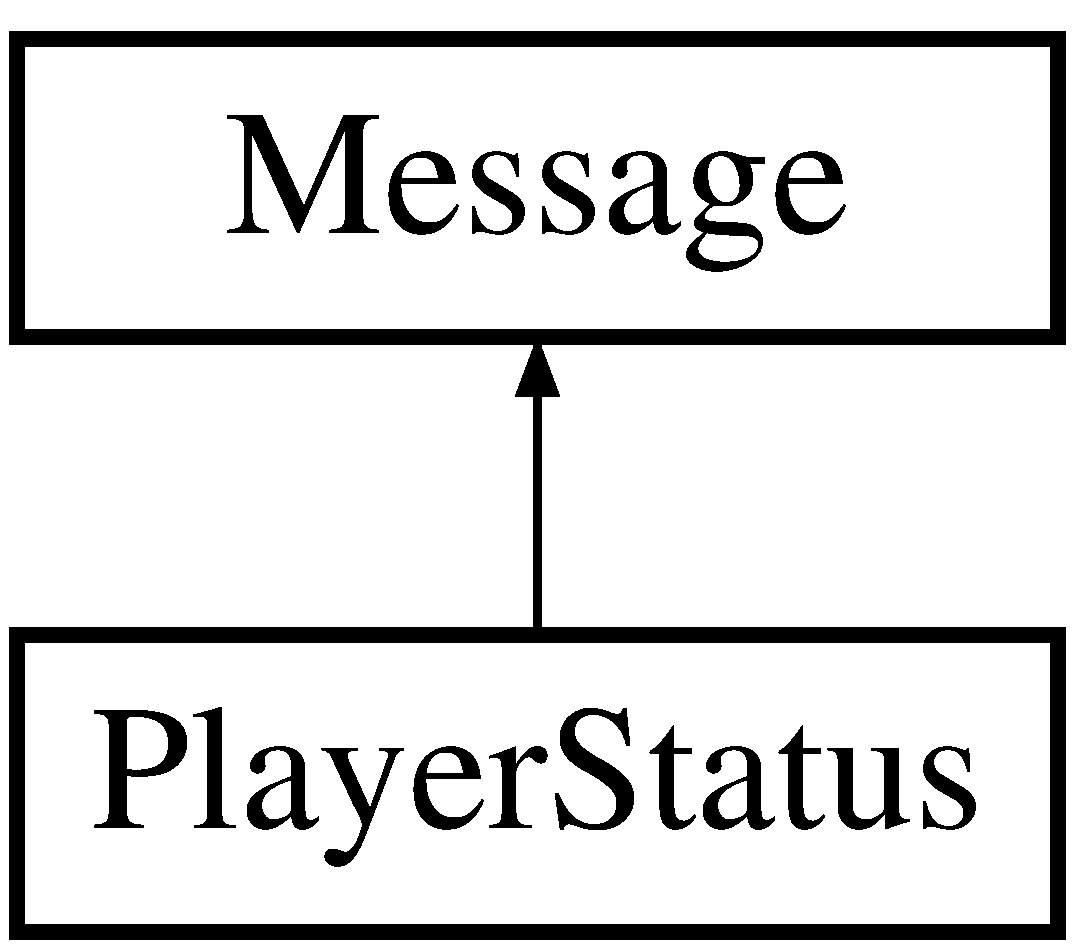
\includegraphics[height=2.000000cm]{class_player_status}
\end{center}
\end{figure}
\subsection*{Public Member Functions}
\begin{DoxyCompactItemize}
\item 
\hyperlink{class_player_status_a1477f7baca38dc993cb832fecb0872f5}{Player\-Status} ()
\item 
virtual \hyperlink{class_player_status_a8ad65fd082d01ec351d2e576c03b6c0c}{$\sim$\-Player\-Status} ()
\item 
\hyperlink{class_player_status_a8869154aa29284c289564424ca3d81ca}{Player\-Status} (const \hyperlink{class_player_status}{Player\-Status} \&from)
\item 
\hyperlink{class_player_status}{Player\-Status} \& \hyperlink{class_player_status_ad1150a8edc62109ee1ae7417ee476025}{operator=} (const \hyperlink{class_player_status}{Player\-Status} \&from)
\item 
const \\*
\-::google\-::protobuf\-::\-Unknown\-Field\-Set \& \hyperlink{class_player_status_ab7eee10cff7a50c69725159cf290352c}{unknown\-\_\-fields} () const 
\item 
inline\-::google\-::protobuf\-::\-Unknown\-Field\-Set $\ast$ \hyperlink{class_player_status_abed60d55b4bcce83f29d29c1fe9c768e}{mutable\-\_\-unknown\-\_\-fields} ()
\item 
void \hyperlink{class_player_status_a54451e7148d8bfc7ec996ff95296fbb6}{Swap} (\hyperlink{class_player_status}{Player\-Status} $\ast$other)
\item 
\hyperlink{class_player_status}{Player\-Status} $\ast$ \hyperlink{class_player_status_a5f463e20d20428030476245da9d6d52a}{New} () const 
\item 
\hyperlink{class_player_status}{Player\-Status} $\ast$ \hyperlink{class_player_status_a05abd2f0659614a206ca97ac55cfece0}{New} (\-::google\-::protobuf\-::\-Arena $\ast$arena) const 
\item 
void \hyperlink{class_player_status_af3573249f694a353dcfc7047af795730}{Copy\-From} (const \-::google\-::protobuf\-::\-Message \&from)
\item 
void \hyperlink{class_player_status_abf908695ca2070f30ac7289cd5b6ebc9}{Merge\-From} (const \-::google\-::protobuf\-::\-Message \&from)
\item 
void \hyperlink{class_player_status_a59b13d7a4c4d170bbf103ce9650c76af}{Copy\-From} (const \hyperlink{class_player_status}{Player\-Status} \&from)
\item 
void \hyperlink{class_player_status_a299630c8c40e216a67c3a6f7b9af6e71}{Merge\-From} (const \hyperlink{class_player_status}{Player\-Status} \&from)
\item 
void \hyperlink{class_player_status_a869a9837799852d1d5c4c30cefd495a8}{Clear} ()
\item 
bool \hyperlink{class_player_status_af77a5dbd97872bc975b8b3a0804ea84e}{Is\-Initialized} () const 
\item 
int \hyperlink{class_player_status_a1b4ef50237a9ec0e43325b60083c0660}{Byte\-Size} () const 
\item 
bool \hyperlink{class_player_status_a9616d3aa3ea0be9520e04b51540de136}{Merge\-Partial\-From\-Coded\-Stream} (\-::google\-::protobuf\-::io\-::\-Coded\-Input\-Stream $\ast$input)
\item 
void \hyperlink{class_player_status_a35cd38f2703b11a1966b345b83235917}{Serialize\-With\-Cached\-Sizes} (\-::google\-::protobuf\-::io\-::\-Coded\-Output\-Stream $\ast$output) const 
\item 
\-::google\-::protobuf\-::uint8 $\ast$ \hyperlink{class_player_status_a1886db442fd6e7d70710692d9f0c78ec}{Serialize\-With\-Cached\-Sizes\-To\-Array} (\-::google\-::protobuf\-::uint8 $\ast$output) const 
\item 
int \hyperlink{class_player_status_ab8f15398fd55d9c9beb952376db309c1}{Get\-Cached\-Size} () const 
\item 
\-::google\-::protobuf\-::\-Metadata \hyperlink{class_player_status_a3f6074ac088b9fdfc53961998908498c}{Get\-Metadata} () const 
\item 
bool \hyperlink{class_player_status_a87a6e0694705a02266e19a0431dcc8bd}{has\-\_\-num\-\_\-of\-\_\-player} () const 
\item 
void \hyperlink{class_player_status_a4ad8dc674124a3f60415fdc42f9bb145}{clear\-\_\-num\-\_\-of\-\_\-player} ()
\item 
inline\-::google\-::protobuf\-::int32 \hyperlink{class_player_status_a44687f76d5e97b584660fbab2441b069}{num\-\_\-of\-\_\-player} () const 
\item 
void \hyperlink{class_player_status_a629692934e938d6f22d32ea5e595d788}{set\-\_\-num\-\_\-of\-\_\-player} (\-::google\-::protobuf\-::int32 value)
\item 
bool \hyperlink{class_player_status_ac13cb145ece1931f7cafb4ce6190a77f}{has\-\_\-playerpoints} () const 
\item 
void \hyperlink{class_player_status_aef1e2bbad803ac9ddcd33b3ee3f6bd98}{clear\-\_\-playerpoints} ()
\item 
inline\-::google\-::protobuf\-::int32 \hyperlink{class_player_status_a573842d49971874f154de31bcf52efb9}{playerpoints} () const 
\item 
void \hyperlink{class_player_status_a368618e48276a5d8bc2744578b0316cf}{set\-\_\-playerpoints} (\-::google\-::protobuf\-::int32 value)
\item 
bool \hyperlink{class_player_status_ad64bd569ef1e245fd8a014fcd8f04090}{has\-\_\-playerlife} () const 
\item 
void \hyperlink{class_player_status_a11691b2df689ecf3e2326e1b79c7abad}{clear\-\_\-playerlife} ()
\item 
inline\-::google\-::protobuf\-::int32 \hyperlink{class_player_status_afa7a932b0873514837c8510653e5af8e}{playerlife} () const 
\item 
void \hyperlink{class_player_status_a0df038d9ba5b74adf38613ebc31145bb}{set\-\_\-playerlife} (\-::google\-::protobuf\-::int32 value)
\item 
bool \hyperlink{class_player_status_ad9ced9478424750043236d941be787ac}{has\-\_\-isdead} () const 
\item 
void \hyperlink{class_player_status_a10a63552e37c6ed389f628b4f0b23e09}{clear\-\_\-isdead} ()
\item 
bool \hyperlink{class_player_status_ab2bab29066cc2dfe5a955ca97b8399df}{isdead} () const 
\item 
void \hyperlink{class_player_status_a5455c655f5e9ef116b8a9c0d01ae6bf9}{set\-\_\-isdead} (bool value)
\item 
bool \hyperlink{class_player_status_aedd0ba4ab7fc76b8a65e0fd5a23c2050}{has\-\_\-numofmunition} () const 
\item 
void \hyperlink{class_player_status_a6ba4592adf5601fb83dd30f4795782ae}{clear\-\_\-numofmunition} ()
\item 
inline\-::google\-::protobuf\-::int32 \hyperlink{class_player_status_ab687554cb754eb588560c88fe4463c9c}{numofmunition} () const 
\item 
void \hyperlink{class_player_status_a4c2212ad0929db7347b7cd7b4dcb9f81}{set\-\_\-numofmunition} (\-::google\-::protobuf\-::int32 value)
\item 
bool \hyperlink{class_player_status_a4bab5a0a30765503c645b4350bb7fde8}{has\-\_\-typeofmunition} () const 
\item 
void \hyperlink{class_player_status_ad37747c7d34b4104483fae73f48891a5}{clear\-\_\-typeofmunition} ()
\item 
inline\-::google\-::protobuf\-::int32 \hyperlink{class_player_status_a7438b0ef8fc2f48f1a015dc0366c187b}{typeofmunition} () const 
\item 
void \hyperlink{class_player_status_a71302f023e61c011a72a257c8ea5cb6e}{set\-\_\-typeofmunition} (\-::google\-::protobuf\-::int32 value)
\item 
bool \hyperlink{class_player_status_a5fd8e8bc7150715dff17890d0f2ba2b5}{has\-\_\-combustible} () const 
\item 
void \hyperlink{class_player_status_adbfd6aeb497ff46eeec87cbb9241b45e}{clear\-\_\-combustible} ()
\item 
inline\-::google\-::protobuf\-::int32 \hyperlink{class_player_status_abffad29c44d3df78f1f0e16da159a570}{combustible} () const 
\item 
void \hyperlink{class_player_status_a6ccd28b6811ebadefa2378881a22fc14}{set\-\_\-combustible} (\-::google\-::protobuf\-::int32 value)
\end{DoxyCompactItemize}
\subsection*{Static Public Member Functions}
\begin{DoxyCompactItemize}
\item 
static const \\*
\-::google\-::protobuf\-::\-Descriptor $\ast$ \hyperlink{class_player_status_ab7af70a3b8976e2a2971f67dd88d2ee0}{descriptor} ()
\item 
static const \hyperlink{class_player_status}{Player\-Status} \& \hyperlink{class_player_status_a48e587242903b11af6171a3307bdac91}{default\-\_\-instance} ()
\end{DoxyCompactItemize}
\subsection*{Static Public Attributes}
\begin{DoxyCompactItemize}
\item 
static const int \hyperlink{class_player_status_a1420e7c20cf4424d3c25d4774f3b02a3}{k\-N\-U\-M\-O\-F\-P\-L\-A\-Y\-E\-R\-Field\-Number} = 1
\item 
static const int \hyperlink{class_player_status_acf4acbabe53753e3554a06ef928683a0}{k\-Player\-Points\-Field\-Number} = 2
\item 
static const int \hyperlink{class_player_status_a335a1328cd6c4be06ecb9c13e6ea9abf}{k\-Player\-Life\-Field\-Number} = 3
\item 
static const int \hyperlink{class_player_status_aa4c5235c27c896e7f2723c6c74a218a4}{k\-Is\-Dead\-Field\-Number} = 4
\item 
static const int \hyperlink{class_player_status_a1652b02aee1015ef64aeb10192344360}{k\-Num\-Of\-Munition\-Field\-Number} = 5
\item 
static const int \hyperlink{class_player_status_a5afa1140c6bf97e7a35b8c15a529022e}{k\-Type\-Of\-Munition\-Field\-Number} = 6
\item 
static const int \hyperlink{class_player_status_a79b1d6540d45cbfb5f2597a4321a139c}{k\-Combustible\-Field\-Number} = 7
\end{DoxyCompactItemize}
\subsection*{Friends}
\begin{DoxyCompactItemize}
\item 
void \hyperlink{class_player_status_a290128592e152c8359d6cbd8ddcf6149}{protobuf\-\_\-\-Add\-Desc\-\_\-\-Player\-Status\-\_\-2eproto} ()
\item 
void \hyperlink{class_player_status_a94feb01d8332b50adabb4d789258c0cc}{protobuf\-\_\-\-Assign\-Desc\-\_\-\-Player\-Status\-\_\-2eproto} ()
\item 
void \hyperlink{class_player_status_a8f9c4c72438a0dd5519155e999949dfc}{protobuf\-\_\-\-Shutdown\-File\-\_\-\-Player\-Status\-\_\-2eproto} ()
\end{DoxyCompactItemize}


\subsection{Constructor \& Destructor Documentation}
\hypertarget{class_player_status_a1477f7baca38dc993cb832fecb0872f5}{\index{Player\-Status@{Player\-Status}!Player\-Status@{Player\-Status}}
\index{Player\-Status@{Player\-Status}!PlayerStatus@{Player\-Status}}
\subsubsection[{Player\-Status}]{\setlength{\rightskip}{0pt plus 5cm}Player\-Status\-::\-Player\-Status (
\begin{DoxyParamCaption}
{}
\end{DoxyParamCaption}
)}}\label{class_player_status_a1477f7baca38dc993cb832fecb0872f5}
\hypertarget{class_player_status_a8ad65fd082d01ec351d2e576c03b6c0c}{\index{Player\-Status@{Player\-Status}!$\sim$\-Player\-Status@{$\sim$\-Player\-Status}}
\index{$\sim$\-Player\-Status@{$\sim$\-Player\-Status}!PlayerStatus@{Player\-Status}}
\subsubsection[{$\sim$\-Player\-Status}]{\setlength{\rightskip}{0pt plus 5cm}Player\-Status\-::$\sim$\-Player\-Status (
\begin{DoxyParamCaption}
{}
\end{DoxyParamCaption}
)\hspace{0.3cm}{\ttfamily [virtual]}}}\label{class_player_status_a8ad65fd082d01ec351d2e576c03b6c0c}
\hypertarget{class_player_status_a8869154aa29284c289564424ca3d81ca}{\index{Player\-Status@{Player\-Status}!Player\-Status@{Player\-Status}}
\index{Player\-Status@{Player\-Status}!PlayerStatus@{Player\-Status}}
\subsubsection[{Player\-Status}]{\setlength{\rightskip}{0pt plus 5cm}Player\-Status\-::\-Player\-Status (
\begin{DoxyParamCaption}
\item[{const {\bf Player\-Status} \&}]{from}
\end{DoxyParamCaption}
)}}\label{class_player_status_a8869154aa29284c289564424ca3d81ca}


\subsection{Member Function Documentation}
\hypertarget{class_player_status_a1b4ef50237a9ec0e43325b60083c0660}{\index{Player\-Status@{Player\-Status}!Byte\-Size@{Byte\-Size}}
\index{Byte\-Size@{Byte\-Size}!PlayerStatus@{Player\-Status}}
\subsubsection[{Byte\-Size}]{\setlength{\rightskip}{0pt plus 5cm}int Player\-Status\-::\-Byte\-Size (
\begin{DoxyParamCaption}
{}
\end{DoxyParamCaption}
) const}}\label{class_player_status_a1b4ef50237a9ec0e43325b60083c0660}
\hypertarget{class_player_status_a869a9837799852d1d5c4c30cefd495a8}{\index{Player\-Status@{Player\-Status}!Clear@{Clear}}
\index{Clear@{Clear}!PlayerStatus@{Player\-Status}}
\subsubsection[{Clear}]{\setlength{\rightskip}{0pt plus 5cm}void Player\-Status\-::\-Clear (
\begin{DoxyParamCaption}
{}
\end{DoxyParamCaption}
)}}\label{class_player_status_a869a9837799852d1d5c4c30cefd495a8}
\hypertarget{class_player_status_adbfd6aeb497ff46eeec87cbb9241b45e}{\index{Player\-Status@{Player\-Status}!clear\-\_\-combustible@{clear\-\_\-combustible}}
\index{clear\-\_\-combustible@{clear\-\_\-combustible}!PlayerStatus@{Player\-Status}}
\subsubsection[{clear\-\_\-combustible}]{\setlength{\rightskip}{0pt plus 5cm}void Player\-Status\-::clear\-\_\-combustible (
\begin{DoxyParamCaption}
{}
\end{DoxyParamCaption}
)\hspace{0.3cm}{\ttfamily [inline]}}}\label{class_player_status_adbfd6aeb497ff46eeec87cbb9241b45e}
\hypertarget{class_player_status_a10a63552e37c6ed389f628b4f0b23e09}{\index{Player\-Status@{Player\-Status}!clear\-\_\-isdead@{clear\-\_\-isdead}}
\index{clear\-\_\-isdead@{clear\-\_\-isdead}!PlayerStatus@{Player\-Status}}
\subsubsection[{clear\-\_\-isdead}]{\setlength{\rightskip}{0pt plus 5cm}void Player\-Status\-::clear\-\_\-isdead (
\begin{DoxyParamCaption}
{}
\end{DoxyParamCaption}
)\hspace{0.3cm}{\ttfamily [inline]}}}\label{class_player_status_a10a63552e37c6ed389f628b4f0b23e09}
\hypertarget{class_player_status_a4ad8dc674124a3f60415fdc42f9bb145}{\index{Player\-Status@{Player\-Status}!clear\-\_\-num\-\_\-of\-\_\-player@{clear\-\_\-num\-\_\-of\-\_\-player}}
\index{clear\-\_\-num\-\_\-of\-\_\-player@{clear\-\_\-num\-\_\-of\-\_\-player}!PlayerStatus@{Player\-Status}}
\subsubsection[{clear\-\_\-num\-\_\-of\-\_\-player}]{\setlength{\rightskip}{0pt plus 5cm}void Player\-Status\-::clear\-\_\-num\-\_\-of\-\_\-player (
\begin{DoxyParamCaption}
{}
\end{DoxyParamCaption}
)\hspace{0.3cm}{\ttfamily [inline]}}}\label{class_player_status_a4ad8dc674124a3f60415fdc42f9bb145}
\hypertarget{class_player_status_a6ba4592adf5601fb83dd30f4795782ae}{\index{Player\-Status@{Player\-Status}!clear\-\_\-numofmunition@{clear\-\_\-numofmunition}}
\index{clear\-\_\-numofmunition@{clear\-\_\-numofmunition}!PlayerStatus@{Player\-Status}}
\subsubsection[{clear\-\_\-numofmunition}]{\setlength{\rightskip}{0pt plus 5cm}void Player\-Status\-::clear\-\_\-numofmunition (
\begin{DoxyParamCaption}
{}
\end{DoxyParamCaption}
)\hspace{0.3cm}{\ttfamily [inline]}}}\label{class_player_status_a6ba4592adf5601fb83dd30f4795782ae}
\hypertarget{class_player_status_a11691b2df689ecf3e2326e1b79c7abad}{\index{Player\-Status@{Player\-Status}!clear\-\_\-playerlife@{clear\-\_\-playerlife}}
\index{clear\-\_\-playerlife@{clear\-\_\-playerlife}!PlayerStatus@{Player\-Status}}
\subsubsection[{clear\-\_\-playerlife}]{\setlength{\rightskip}{0pt plus 5cm}void Player\-Status\-::clear\-\_\-playerlife (
\begin{DoxyParamCaption}
{}
\end{DoxyParamCaption}
)\hspace{0.3cm}{\ttfamily [inline]}}}\label{class_player_status_a11691b2df689ecf3e2326e1b79c7abad}
\hypertarget{class_player_status_aef1e2bbad803ac9ddcd33b3ee3f6bd98}{\index{Player\-Status@{Player\-Status}!clear\-\_\-playerpoints@{clear\-\_\-playerpoints}}
\index{clear\-\_\-playerpoints@{clear\-\_\-playerpoints}!PlayerStatus@{Player\-Status}}
\subsubsection[{clear\-\_\-playerpoints}]{\setlength{\rightskip}{0pt plus 5cm}void Player\-Status\-::clear\-\_\-playerpoints (
\begin{DoxyParamCaption}
{}
\end{DoxyParamCaption}
)\hspace{0.3cm}{\ttfamily [inline]}}}\label{class_player_status_aef1e2bbad803ac9ddcd33b3ee3f6bd98}
\hypertarget{class_player_status_ad37747c7d34b4104483fae73f48891a5}{\index{Player\-Status@{Player\-Status}!clear\-\_\-typeofmunition@{clear\-\_\-typeofmunition}}
\index{clear\-\_\-typeofmunition@{clear\-\_\-typeofmunition}!PlayerStatus@{Player\-Status}}
\subsubsection[{clear\-\_\-typeofmunition}]{\setlength{\rightskip}{0pt plus 5cm}void Player\-Status\-::clear\-\_\-typeofmunition (
\begin{DoxyParamCaption}
{}
\end{DoxyParamCaption}
)\hspace{0.3cm}{\ttfamily [inline]}}}\label{class_player_status_ad37747c7d34b4104483fae73f48891a5}
\hypertarget{class_player_status_abffad29c44d3df78f1f0e16da159a570}{\index{Player\-Status@{Player\-Status}!combustible@{combustible}}
\index{combustible@{combustible}!PlayerStatus@{Player\-Status}}
\subsubsection[{combustible}]{\setlength{\rightskip}{0pt plus 5cm}google\-::protobuf\-::int32 Player\-Status\-::combustible (
\begin{DoxyParamCaption}
{}
\end{DoxyParamCaption}
) const\hspace{0.3cm}{\ttfamily [inline]}}}\label{class_player_status_abffad29c44d3df78f1f0e16da159a570}
\hypertarget{class_player_status_af3573249f694a353dcfc7047af795730}{\index{Player\-Status@{Player\-Status}!Copy\-From@{Copy\-From}}
\index{Copy\-From@{Copy\-From}!PlayerStatus@{Player\-Status}}
\subsubsection[{Copy\-From}]{\setlength{\rightskip}{0pt plus 5cm}void Player\-Status\-::\-Copy\-From (
\begin{DoxyParamCaption}
\item[{const \-::google\-::protobuf\-::\-Message \&}]{from}
\end{DoxyParamCaption}
)}}\label{class_player_status_af3573249f694a353dcfc7047af795730}
\hypertarget{class_player_status_a59b13d7a4c4d170bbf103ce9650c76af}{\index{Player\-Status@{Player\-Status}!Copy\-From@{Copy\-From}}
\index{Copy\-From@{Copy\-From}!PlayerStatus@{Player\-Status}}
\subsubsection[{Copy\-From}]{\setlength{\rightskip}{0pt plus 5cm}void Player\-Status\-::\-Copy\-From (
\begin{DoxyParamCaption}
\item[{const {\bf Player\-Status} \&}]{from}
\end{DoxyParamCaption}
)}}\label{class_player_status_a59b13d7a4c4d170bbf103ce9650c76af}
\hypertarget{class_player_status_a48e587242903b11af6171a3307bdac91}{\index{Player\-Status@{Player\-Status}!default\-\_\-instance@{default\-\_\-instance}}
\index{default\-\_\-instance@{default\-\_\-instance}!PlayerStatus@{Player\-Status}}
\subsubsection[{default\-\_\-instance}]{\setlength{\rightskip}{0pt plus 5cm}const {\bf Player\-Status} \& Player\-Status\-::default\-\_\-instance (
\begin{DoxyParamCaption}
{}
\end{DoxyParamCaption}
)\hspace{0.3cm}{\ttfamily [static]}}}\label{class_player_status_a48e587242903b11af6171a3307bdac91}
\hypertarget{class_player_status_ab7af70a3b8976e2a2971f67dd88d2ee0}{\index{Player\-Status@{Player\-Status}!descriptor@{descriptor}}
\index{descriptor@{descriptor}!PlayerStatus@{Player\-Status}}
\subsubsection[{descriptor}]{\setlength{\rightskip}{0pt plus 5cm}const \-::google\-::protobuf\-::\-Descriptor $\ast$ Player\-Status\-::descriptor (
\begin{DoxyParamCaption}
{}
\end{DoxyParamCaption}
)\hspace{0.3cm}{\ttfamily [static]}}}\label{class_player_status_ab7af70a3b8976e2a2971f67dd88d2ee0}
\hypertarget{class_player_status_ab8f15398fd55d9c9beb952376db309c1}{\index{Player\-Status@{Player\-Status}!Get\-Cached\-Size@{Get\-Cached\-Size}}
\index{Get\-Cached\-Size@{Get\-Cached\-Size}!PlayerStatus@{Player\-Status}}
\subsubsection[{Get\-Cached\-Size}]{\setlength{\rightskip}{0pt plus 5cm}int Player\-Status\-::\-Get\-Cached\-Size (
\begin{DoxyParamCaption}
{}
\end{DoxyParamCaption}
) const\hspace{0.3cm}{\ttfamily [inline]}}}\label{class_player_status_ab8f15398fd55d9c9beb952376db309c1}
\hypertarget{class_player_status_a3f6074ac088b9fdfc53961998908498c}{\index{Player\-Status@{Player\-Status}!Get\-Metadata@{Get\-Metadata}}
\index{Get\-Metadata@{Get\-Metadata}!PlayerStatus@{Player\-Status}}
\subsubsection[{Get\-Metadata}]{\setlength{\rightskip}{0pt plus 5cm}google\-::protobuf\-::\-Metadata Player\-Status\-::\-Get\-Metadata (
\begin{DoxyParamCaption}
{}
\end{DoxyParamCaption}
) const}}\label{class_player_status_a3f6074ac088b9fdfc53961998908498c}
\hypertarget{class_player_status_a5fd8e8bc7150715dff17890d0f2ba2b5}{\index{Player\-Status@{Player\-Status}!has\-\_\-combustible@{has\-\_\-combustible}}
\index{has\-\_\-combustible@{has\-\_\-combustible}!PlayerStatus@{Player\-Status}}
\subsubsection[{has\-\_\-combustible}]{\setlength{\rightskip}{0pt plus 5cm}bool Player\-Status\-::has\-\_\-combustible (
\begin{DoxyParamCaption}
{}
\end{DoxyParamCaption}
) const\hspace{0.3cm}{\ttfamily [inline]}}}\label{class_player_status_a5fd8e8bc7150715dff17890d0f2ba2b5}
\hypertarget{class_player_status_ad9ced9478424750043236d941be787ac}{\index{Player\-Status@{Player\-Status}!has\-\_\-isdead@{has\-\_\-isdead}}
\index{has\-\_\-isdead@{has\-\_\-isdead}!PlayerStatus@{Player\-Status}}
\subsubsection[{has\-\_\-isdead}]{\setlength{\rightskip}{0pt plus 5cm}bool Player\-Status\-::has\-\_\-isdead (
\begin{DoxyParamCaption}
{}
\end{DoxyParamCaption}
) const\hspace{0.3cm}{\ttfamily [inline]}}}\label{class_player_status_ad9ced9478424750043236d941be787ac}
\hypertarget{class_player_status_a87a6e0694705a02266e19a0431dcc8bd}{\index{Player\-Status@{Player\-Status}!has\-\_\-num\-\_\-of\-\_\-player@{has\-\_\-num\-\_\-of\-\_\-player}}
\index{has\-\_\-num\-\_\-of\-\_\-player@{has\-\_\-num\-\_\-of\-\_\-player}!PlayerStatus@{Player\-Status}}
\subsubsection[{has\-\_\-num\-\_\-of\-\_\-player}]{\setlength{\rightskip}{0pt plus 5cm}bool Player\-Status\-::has\-\_\-num\-\_\-of\-\_\-player (
\begin{DoxyParamCaption}
{}
\end{DoxyParamCaption}
) const\hspace{0.3cm}{\ttfamily [inline]}}}\label{class_player_status_a87a6e0694705a02266e19a0431dcc8bd}
\hypertarget{class_player_status_aedd0ba4ab7fc76b8a65e0fd5a23c2050}{\index{Player\-Status@{Player\-Status}!has\-\_\-numofmunition@{has\-\_\-numofmunition}}
\index{has\-\_\-numofmunition@{has\-\_\-numofmunition}!PlayerStatus@{Player\-Status}}
\subsubsection[{has\-\_\-numofmunition}]{\setlength{\rightskip}{0pt plus 5cm}bool Player\-Status\-::has\-\_\-numofmunition (
\begin{DoxyParamCaption}
{}
\end{DoxyParamCaption}
) const\hspace{0.3cm}{\ttfamily [inline]}}}\label{class_player_status_aedd0ba4ab7fc76b8a65e0fd5a23c2050}
\hypertarget{class_player_status_ad64bd569ef1e245fd8a014fcd8f04090}{\index{Player\-Status@{Player\-Status}!has\-\_\-playerlife@{has\-\_\-playerlife}}
\index{has\-\_\-playerlife@{has\-\_\-playerlife}!PlayerStatus@{Player\-Status}}
\subsubsection[{has\-\_\-playerlife}]{\setlength{\rightskip}{0pt plus 5cm}bool Player\-Status\-::has\-\_\-playerlife (
\begin{DoxyParamCaption}
{}
\end{DoxyParamCaption}
) const\hspace{0.3cm}{\ttfamily [inline]}}}\label{class_player_status_ad64bd569ef1e245fd8a014fcd8f04090}
\hypertarget{class_player_status_ac13cb145ece1931f7cafb4ce6190a77f}{\index{Player\-Status@{Player\-Status}!has\-\_\-playerpoints@{has\-\_\-playerpoints}}
\index{has\-\_\-playerpoints@{has\-\_\-playerpoints}!PlayerStatus@{Player\-Status}}
\subsubsection[{has\-\_\-playerpoints}]{\setlength{\rightskip}{0pt plus 5cm}bool Player\-Status\-::has\-\_\-playerpoints (
\begin{DoxyParamCaption}
{}
\end{DoxyParamCaption}
) const\hspace{0.3cm}{\ttfamily [inline]}}}\label{class_player_status_ac13cb145ece1931f7cafb4ce6190a77f}
\hypertarget{class_player_status_a4bab5a0a30765503c645b4350bb7fde8}{\index{Player\-Status@{Player\-Status}!has\-\_\-typeofmunition@{has\-\_\-typeofmunition}}
\index{has\-\_\-typeofmunition@{has\-\_\-typeofmunition}!PlayerStatus@{Player\-Status}}
\subsubsection[{has\-\_\-typeofmunition}]{\setlength{\rightskip}{0pt plus 5cm}bool Player\-Status\-::has\-\_\-typeofmunition (
\begin{DoxyParamCaption}
{}
\end{DoxyParamCaption}
) const\hspace{0.3cm}{\ttfamily [inline]}}}\label{class_player_status_a4bab5a0a30765503c645b4350bb7fde8}
\hypertarget{class_player_status_ab2bab29066cc2dfe5a955ca97b8399df}{\index{Player\-Status@{Player\-Status}!isdead@{isdead}}
\index{isdead@{isdead}!PlayerStatus@{Player\-Status}}
\subsubsection[{isdead}]{\setlength{\rightskip}{0pt plus 5cm}bool Player\-Status\-::isdead (
\begin{DoxyParamCaption}
{}
\end{DoxyParamCaption}
) const\hspace{0.3cm}{\ttfamily [inline]}}}\label{class_player_status_ab2bab29066cc2dfe5a955ca97b8399df}
\hypertarget{class_player_status_af77a5dbd97872bc975b8b3a0804ea84e}{\index{Player\-Status@{Player\-Status}!Is\-Initialized@{Is\-Initialized}}
\index{Is\-Initialized@{Is\-Initialized}!PlayerStatus@{Player\-Status}}
\subsubsection[{Is\-Initialized}]{\setlength{\rightskip}{0pt plus 5cm}bool Player\-Status\-::\-Is\-Initialized (
\begin{DoxyParamCaption}
{}
\end{DoxyParamCaption}
) const}}\label{class_player_status_af77a5dbd97872bc975b8b3a0804ea84e}
\hypertarget{class_player_status_abf908695ca2070f30ac7289cd5b6ebc9}{\index{Player\-Status@{Player\-Status}!Merge\-From@{Merge\-From}}
\index{Merge\-From@{Merge\-From}!PlayerStatus@{Player\-Status}}
\subsubsection[{Merge\-From}]{\setlength{\rightskip}{0pt plus 5cm}void Player\-Status\-::\-Merge\-From (
\begin{DoxyParamCaption}
\item[{const \-::google\-::protobuf\-::\-Message \&}]{from}
\end{DoxyParamCaption}
)}}\label{class_player_status_abf908695ca2070f30ac7289cd5b6ebc9}
\hypertarget{class_player_status_a299630c8c40e216a67c3a6f7b9af6e71}{\index{Player\-Status@{Player\-Status}!Merge\-From@{Merge\-From}}
\index{Merge\-From@{Merge\-From}!PlayerStatus@{Player\-Status}}
\subsubsection[{Merge\-From}]{\setlength{\rightskip}{0pt plus 5cm}void Player\-Status\-::\-Merge\-From (
\begin{DoxyParamCaption}
\item[{const {\bf Player\-Status} \&}]{from}
\end{DoxyParamCaption}
)}}\label{class_player_status_a299630c8c40e216a67c3a6f7b9af6e71}
\hypertarget{class_player_status_a9616d3aa3ea0be9520e04b51540de136}{\index{Player\-Status@{Player\-Status}!Merge\-Partial\-From\-Coded\-Stream@{Merge\-Partial\-From\-Coded\-Stream}}
\index{Merge\-Partial\-From\-Coded\-Stream@{Merge\-Partial\-From\-Coded\-Stream}!PlayerStatus@{Player\-Status}}
\subsubsection[{Merge\-Partial\-From\-Coded\-Stream}]{\setlength{\rightskip}{0pt plus 5cm}bool Player\-Status\-::\-Merge\-Partial\-From\-Coded\-Stream (
\begin{DoxyParamCaption}
\item[{\-::google\-::protobuf\-::io\-::\-Coded\-Input\-Stream $\ast$}]{input}
\end{DoxyParamCaption}
)}}\label{class_player_status_a9616d3aa3ea0be9520e04b51540de136}
\hypertarget{class_player_status_abed60d55b4bcce83f29d29c1fe9c768e}{\index{Player\-Status@{Player\-Status}!mutable\-\_\-unknown\-\_\-fields@{mutable\-\_\-unknown\-\_\-fields}}
\index{mutable\-\_\-unknown\-\_\-fields@{mutable\-\_\-unknown\-\_\-fields}!PlayerStatus@{Player\-Status}}
\subsubsection[{mutable\-\_\-unknown\-\_\-fields}]{\setlength{\rightskip}{0pt plus 5cm}inline \-::google\-::protobuf\-::\-Unknown\-Field\-Set$\ast$ Player\-Status\-::mutable\-\_\-unknown\-\_\-fields (
\begin{DoxyParamCaption}
{}
\end{DoxyParamCaption}
)\hspace{0.3cm}{\ttfamily [inline]}}}\label{class_player_status_abed60d55b4bcce83f29d29c1fe9c768e}
\hypertarget{class_player_status_a5f463e20d20428030476245da9d6d52a}{\index{Player\-Status@{Player\-Status}!New@{New}}
\index{New@{New}!PlayerStatus@{Player\-Status}}
\subsubsection[{New}]{\setlength{\rightskip}{0pt plus 5cm}{\bf Player\-Status}$\ast$ Player\-Status\-::\-New (
\begin{DoxyParamCaption}
{}
\end{DoxyParamCaption}
) const\hspace{0.3cm}{\ttfamily [inline]}}}\label{class_player_status_a5f463e20d20428030476245da9d6d52a}
\hypertarget{class_player_status_a05abd2f0659614a206ca97ac55cfece0}{\index{Player\-Status@{Player\-Status}!New@{New}}
\index{New@{New}!PlayerStatus@{Player\-Status}}
\subsubsection[{New}]{\setlength{\rightskip}{0pt plus 5cm}{\bf Player\-Status} $\ast$ Player\-Status\-::\-New (
\begin{DoxyParamCaption}
\item[{\-::google\-::protobuf\-::\-Arena $\ast$}]{arena}
\end{DoxyParamCaption}
) const}}\label{class_player_status_a05abd2f0659614a206ca97ac55cfece0}
\hypertarget{class_player_status_a44687f76d5e97b584660fbab2441b069}{\index{Player\-Status@{Player\-Status}!num\-\_\-of\-\_\-player@{num\-\_\-of\-\_\-player}}
\index{num\-\_\-of\-\_\-player@{num\-\_\-of\-\_\-player}!PlayerStatus@{Player\-Status}}
\subsubsection[{num\-\_\-of\-\_\-player}]{\setlength{\rightskip}{0pt plus 5cm}google\-::protobuf\-::int32 Player\-Status\-::num\-\_\-of\-\_\-player (
\begin{DoxyParamCaption}
{}
\end{DoxyParamCaption}
) const\hspace{0.3cm}{\ttfamily [inline]}}}\label{class_player_status_a44687f76d5e97b584660fbab2441b069}
\hypertarget{class_player_status_ab687554cb754eb588560c88fe4463c9c}{\index{Player\-Status@{Player\-Status}!numofmunition@{numofmunition}}
\index{numofmunition@{numofmunition}!PlayerStatus@{Player\-Status}}
\subsubsection[{numofmunition}]{\setlength{\rightskip}{0pt plus 5cm}google\-::protobuf\-::int32 Player\-Status\-::numofmunition (
\begin{DoxyParamCaption}
{}
\end{DoxyParamCaption}
) const\hspace{0.3cm}{\ttfamily [inline]}}}\label{class_player_status_ab687554cb754eb588560c88fe4463c9c}
\hypertarget{class_player_status_ad1150a8edc62109ee1ae7417ee476025}{\index{Player\-Status@{Player\-Status}!operator=@{operator=}}
\index{operator=@{operator=}!PlayerStatus@{Player\-Status}}
\subsubsection[{operator=}]{\setlength{\rightskip}{0pt plus 5cm}{\bf Player\-Status}\& Player\-Status\-::operator= (
\begin{DoxyParamCaption}
\item[{const {\bf Player\-Status} \&}]{from}
\end{DoxyParamCaption}
)\hspace{0.3cm}{\ttfamily [inline]}}}\label{class_player_status_ad1150a8edc62109ee1ae7417ee476025}
\hypertarget{class_player_status_afa7a932b0873514837c8510653e5af8e}{\index{Player\-Status@{Player\-Status}!playerlife@{playerlife}}
\index{playerlife@{playerlife}!PlayerStatus@{Player\-Status}}
\subsubsection[{playerlife}]{\setlength{\rightskip}{0pt plus 5cm}google\-::protobuf\-::int32 Player\-Status\-::playerlife (
\begin{DoxyParamCaption}
{}
\end{DoxyParamCaption}
) const\hspace{0.3cm}{\ttfamily [inline]}}}\label{class_player_status_afa7a932b0873514837c8510653e5af8e}
\hypertarget{class_player_status_a573842d49971874f154de31bcf52efb9}{\index{Player\-Status@{Player\-Status}!playerpoints@{playerpoints}}
\index{playerpoints@{playerpoints}!PlayerStatus@{Player\-Status}}
\subsubsection[{playerpoints}]{\setlength{\rightskip}{0pt plus 5cm}google\-::protobuf\-::int32 Player\-Status\-::playerpoints (
\begin{DoxyParamCaption}
{}
\end{DoxyParamCaption}
) const\hspace{0.3cm}{\ttfamily [inline]}}}\label{class_player_status_a573842d49971874f154de31bcf52efb9}
\hypertarget{class_player_status_a35cd38f2703b11a1966b345b83235917}{\index{Player\-Status@{Player\-Status}!Serialize\-With\-Cached\-Sizes@{Serialize\-With\-Cached\-Sizes}}
\index{Serialize\-With\-Cached\-Sizes@{Serialize\-With\-Cached\-Sizes}!PlayerStatus@{Player\-Status}}
\subsubsection[{Serialize\-With\-Cached\-Sizes}]{\setlength{\rightskip}{0pt plus 5cm}void Player\-Status\-::\-Serialize\-With\-Cached\-Sizes (
\begin{DoxyParamCaption}
\item[{\-::google\-::protobuf\-::io\-::\-Coded\-Output\-Stream $\ast$}]{output}
\end{DoxyParamCaption}
) const}}\label{class_player_status_a35cd38f2703b11a1966b345b83235917}
\hypertarget{class_player_status_a1886db442fd6e7d70710692d9f0c78ec}{\index{Player\-Status@{Player\-Status}!Serialize\-With\-Cached\-Sizes\-To\-Array@{Serialize\-With\-Cached\-Sizes\-To\-Array}}
\index{Serialize\-With\-Cached\-Sizes\-To\-Array@{Serialize\-With\-Cached\-Sizes\-To\-Array}!PlayerStatus@{Player\-Status}}
\subsubsection[{Serialize\-With\-Cached\-Sizes\-To\-Array}]{\setlength{\rightskip}{0pt plus 5cm}google\-::protobuf\-::uint8 $\ast$ Player\-Status\-::\-Serialize\-With\-Cached\-Sizes\-To\-Array (
\begin{DoxyParamCaption}
\item[{\-::google\-::protobuf\-::uint8 $\ast$}]{output}
\end{DoxyParamCaption}
) const}}\label{class_player_status_a1886db442fd6e7d70710692d9f0c78ec}
\hypertarget{class_player_status_a6ccd28b6811ebadefa2378881a22fc14}{\index{Player\-Status@{Player\-Status}!set\-\_\-combustible@{set\-\_\-combustible}}
\index{set\-\_\-combustible@{set\-\_\-combustible}!PlayerStatus@{Player\-Status}}
\subsubsection[{set\-\_\-combustible}]{\setlength{\rightskip}{0pt plus 5cm}void Player\-Status\-::set\-\_\-combustible (
\begin{DoxyParamCaption}
\item[{\-::google\-::protobuf\-::int32}]{value}
\end{DoxyParamCaption}
)\hspace{0.3cm}{\ttfamily [inline]}}}\label{class_player_status_a6ccd28b6811ebadefa2378881a22fc14}
\hypertarget{class_player_status_a5455c655f5e9ef116b8a9c0d01ae6bf9}{\index{Player\-Status@{Player\-Status}!set\-\_\-isdead@{set\-\_\-isdead}}
\index{set\-\_\-isdead@{set\-\_\-isdead}!PlayerStatus@{Player\-Status}}
\subsubsection[{set\-\_\-isdead}]{\setlength{\rightskip}{0pt plus 5cm}void Player\-Status\-::set\-\_\-isdead (
\begin{DoxyParamCaption}
\item[{bool}]{value}
\end{DoxyParamCaption}
)\hspace{0.3cm}{\ttfamily [inline]}}}\label{class_player_status_a5455c655f5e9ef116b8a9c0d01ae6bf9}
\hypertarget{class_player_status_a629692934e938d6f22d32ea5e595d788}{\index{Player\-Status@{Player\-Status}!set\-\_\-num\-\_\-of\-\_\-player@{set\-\_\-num\-\_\-of\-\_\-player}}
\index{set\-\_\-num\-\_\-of\-\_\-player@{set\-\_\-num\-\_\-of\-\_\-player}!PlayerStatus@{Player\-Status}}
\subsubsection[{set\-\_\-num\-\_\-of\-\_\-player}]{\setlength{\rightskip}{0pt plus 5cm}void Player\-Status\-::set\-\_\-num\-\_\-of\-\_\-player (
\begin{DoxyParamCaption}
\item[{\-::google\-::protobuf\-::int32}]{value}
\end{DoxyParamCaption}
)\hspace{0.3cm}{\ttfamily [inline]}}}\label{class_player_status_a629692934e938d6f22d32ea5e595d788}
\hypertarget{class_player_status_a4c2212ad0929db7347b7cd7b4dcb9f81}{\index{Player\-Status@{Player\-Status}!set\-\_\-numofmunition@{set\-\_\-numofmunition}}
\index{set\-\_\-numofmunition@{set\-\_\-numofmunition}!PlayerStatus@{Player\-Status}}
\subsubsection[{set\-\_\-numofmunition}]{\setlength{\rightskip}{0pt plus 5cm}void Player\-Status\-::set\-\_\-numofmunition (
\begin{DoxyParamCaption}
\item[{\-::google\-::protobuf\-::int32}]{value}
\end{DoxyParamCaption}
)\hspace{0.3cm}{\ttfamily [inline]}}}\label{class_player_status_a4c2212ad0929db7347b7cd7b4dcb9f81}
\hypertarget{class_player_status_a0df038d9ba5b74adf38613ebc31145bb}{\index{Player\-Status@{Player\-Status}!set\-\_\-playerlife@{set\-\_\-playerlife}}
\index{set\-\_\-playerlife@{set\-\_\-playerlife}!PlayerStatus@{Player\-Status}}
\subsubsection[{set\-\_\-playerlife}]{\setlength{\rightskip}{0pt plus 5cm}void Player\-Status\-::set\-\_\-playerlife (
\begin{DoxyParamCaption}
\item[{\-::google\-::protobuf\-::int32}]{value}
\end{DoxyParamCaption}
)\hspace{0.3cm}{\ttfamily [inline]}}}\label{class_player_status_a0df038d9ba5b74adf38613ebc31145bb}
\hypertarget{class_player_status_a368618e48276a5d8bc2744578b0316cf}{\index{Player\-Status@{Player\-Status}!set\-\_\-playerpoints@{set\-\_\-playerpoints}}
\index{set\-\_\-playerpoints@{set\-\_\-playerpoints}!PlayerStatus@{Player\-Status}}
\subsubsection[{set\-\_\-playerpoints}]{\setlength{\rightskip}{0pt plus 5cm}void Player\-Status\-::set\-\_\-playerpoints (
\begin{DoxyParamCaption}
\item[{\-::google\-::protobuf\-::int32}]{value}
\end{DoxyParamCaption}
)\hspace{0.3cm}{\ttfamily [inline]}}}\label{class_player_status_a368618e48276a5d8bc2744578b0316cf}
\hypertarget{class_player_status_a71302f023e61c011a72a257c8ea5cb6e}{\index{Player\-Status@{Player\-Status}!set\-\_\-typeofmunition@{set\-\_\-typeofmunition}}
\index{set\-\_\-typeofmunition@{set\-\_\-typeofmunition}!PlayerStatus@{Player\-Status}}
\subsubsection[{set\-\_\-typeofmunition}]{\setlength{\rightskip}{0pt plus 5cm}void Player\-Status\-::set\-\_\-typeofmunition (
\begin{DoxyParamCaption}
\item[{\-::google\-::protobuf\-::int32}]{value}
\end{DoxyParamCaption}
)\hspace{0.3cm}{\ttfamily [inline]}}}\label{class_player_status_a71302f023e61c011a72a257c8ea5cb6e}
\hypertarget{class_player_status_a54451e7148d8bfc7ec996ff95296fbb6}{\index{Player\-Status@{Player\-Status}!Swap@{Swap}}
\index{Swap@{Swap}!PlayerStatus@{Player\-Status}}
\subsubsection[{Swap}]{\setlength{\rightskip}{0pt plus 5cm}void Player\-Status\-::\-Swap (
\begin{DoxyParamCaption}
\item[{{\bf Player\-Status} $\ast$}]{other}
\end{DoxyParamCaption}
)}}\label{class_player_status_a54451e7148d8bfc7ec996ff95296fbb6}
\hypertarget{class_player_status_a7438b0ef8fc2f48f1a015dc0366c187b}{\index{Player\-Status@{Player\-Status}!typeofmunition@{typeofmunition}}
\index{typeofmunition@{typeofmunition}!PlayerStatus@{Player\-Status}}
\subsubsection[{typeofmunition}]{\setlength{\rightskip}{0pt plus 5cm}google\-::protobuf\-::int32 Player\-Status\-::typeofmunition (
\begin{DoxyParamCaption}
{}
\end{DoxyParamCaption}
) const\hspace{0.3cm}{\ttfamily [inline]}}}\label{class_player_status_a7438b0ef8fc2f48f1a015dc0366c187b}
\hypertarget{class_player_status_ab7eee10cff7a50c69725159cf290352c}{\index{Player\-Status@{Player\-Status}!unknown\-\_\-fields@{unknown\-\_\-fields}}
\index{unknown\-\_\-fields@{unknown\-\_\-fields}!PlayerStatus@{Player\-Status}}
\subsubsection[{unknown\-\_\-fields}]{\setlength{\rightskip}{0pt plus 5cm}const \-::google\-::protobuf\-::\-Unknown\-Field\-Set\& Player\-Status\-::unknown\-\_\-fields (
\begin{DoxyParamCaption}
{}
\end{DoxyParamCaption}
) const\hspace{0.3cm}{\ttfamily [inline]}}}\label{class_player_status_ab7eee10cff7a50c69725159cf290352c}


\subsection{Friends And Related Function Documentation}
\hypertarget{class_player_status_a290128592e152c8359d6cbd8ddcf6149}{\index{Player\-Status@{Player\-Status}!protobuf\-\_\-\-Add\-Desc\-\_\-\-Player\-Status\-\_\-2eproto@{protobuf\-\_\-\-Add\-Desc\-\_\-\-Player\-Status\-\_\-2eproto}}
\index{protobuf\-\_\-\-Add\-Desc\-\_\-\-Player\-Status\-\_\-2eproto@{protobuf\-\_\-\-Add\-Desc\-\_\-\-Player\-Status\-\_\-2eproto}!PlayerStatus@{Player\-Status}}
\subsubsection[{protobuf\-\_\-\-Add\-Desc\-\_\-\-Player\-Status\-\_\-2eproto}]{\setlength{\rightskip}{0pt plus 5cm}void protobuf\-\_\-\-Add\-Desc\-\_\-\-Player\-Status\-\_\-2eproto (
\begin{DoxyParamCaption}
{}
\end{DoxyParamCaption}
)\hspace{0.3cm}{\ttfamily [friend]}}}\label{class_player_status_a290128592e152c8359d6cbd8ddcf6149}
\hypertarget{class_player_status_a94feb01d8332b50adabb4d789258c0cc}{\index{Player\-Status@{Player\-Status}!protobuf\-\_\-\-Assign\-Desc\-\_\-\-Player\-Status\-\_\-2eproto@{protobuf\-\_\-\-Assign\-Desc\-\_\-\-Player\-Status\-\_\-2eproto}}
\index{protobuf\-\_\-\-Assign\-Desc\-\_\-\-Player\-Status\-\_\-2eproto@{protobuf\-\_\-\-Assign\-Desc\-\_\-\-Player\-Status\-\_\-2eproto}!PlayerStatus@{Player\-Status}}
\subsubsection[{protobuf\-\_\-\-Assign\-Desc\-\_\-\-Player\-Status\-\_\-2eproto}]{\setlength{\rightskip}{0pt plus 5cm}void protobuf\-\_\-\-Assign\-Desc\-\_\-\-Player\-Status\-\_\-2eproto (
\begin{DoxyParamCaption}
{}
\end{DoxyParamCaption}
)\hspace{0.3cm}{\ttfamily [friend]}}}\label{class_player_status_a94feb01d8332b50adabb4d789258c0cc}
\hypertarget{class_player_status_a8f9c4c72438a0dd5519155e999949dfc}{\index{Player\-Status@{Player\-Status}!protobuf\-\_\-\-Shutdown\-File\-\_\-\-Player\-Status\-\_\-2eproto@{protobuf\-\_\-\-Shutdown\-File\-\_\-\-Player\-Status\-\_\-2eproto}}
\index{protobuf\-\_\-\-Shutdown\-File\-\_\-\-Player\-Status\-\_\-2eproto@{protobuf\-\_\-\-Shutdown\-File\-\_\-\-Player\-Status\-\_\-2eproto}!PlayerStatus@{Player\-Status}}
\subsubsection[{protobuf\-\_\-\-Shutdown\-File\-\_\-\-Player\-Status\-\_\-2eproto}]{\setlength{\rightskip}{0pt plus 5cm}void protobuf\-\_\-\-Shutdown\-File\-\_\-\-Player\-Status\-\_\-2eproto (
\begin{DoxyParamCaption}
{}
\end{DoxyParamCaption}
)\hspace{0.3cm}{\ttfamily [friend]}}}\label{class_player_status_a8f9c4c72438a0dd5519155e999949dfc}


\subsection{Member Data Documentation}
\hypertarget{class_player_status_a79b1d6540d45cbfb5f2597a4321a139c}{\index{Player\-Status@{Player\-Status}!k\-Combustible\-Field\-Number@{k\-Combustible\-Field\-Number}}
\index{k\-Combustible\-Field\-Number@{k\-Combustible\-Field\-Number}!PlayerStatus@{Player\-Status}}
\subsubsection[{k\-Combustible\-Field\-Number}]{\setlength{\rightskip}{0pt plus 5cm}const int Player\-Status\-::k\-Combustible\-Field\-Number = 7\hspace{0.3cm}{\ttfamily [static]}}}\label{class_player_status_a79b1d6540d45cbfb5f2597a4321a139c}
\hypertarget{class_player_status_aa4c5235c27c896e7f2723c6c74a218a4}{\index{Player\-Status@{Player\-Status}!k\-Is\-Dead\-Field\-Number@{k\-Is\-Dead\-Field\-Number}}
\index{k\-Is\-Dead\-Field\-Number@{k\-Is\-Dead\-Field\-Number}!PlayerStatus@{Player\-Status}}
\subsubsection[{k\-Is\-Dead\-Field\-Number}]{\setlength{\rightskip}{0pt plus 5cm}const int Player\-Status\-::k\-Is\-Dead\-Field\-Number = 4\hspace{0.3cm}{\ttfamily [static]}}}\label{class_player_status_aa4c5235c27c896e7f2723c6c74a218a4}
\hypertarget{class_player_status_a1652b02aee1015ef64aeb10192344360}{\index{Player\-Status@{Player\-Status}!k\-Num\-Of\-Munition\-Field\-Number@{k\-Num\-Of\-Munition\-Field\-Number}}
\index{k\-Num\-Of\-Munition\-Field\-Number@{k\-Num\-Of\-Munition\-Field\-Number}!PlayerStatus@{Player\-Status}}
\subsubsection[{k\-Num\-Of\-Munition\-Field\-Number}]{\setlength{\rightskip}{0pt plus 5cm}const int Player\-Status\-::k\-Num\-Of\-Munition\-Field\-Number = 5\hspace{0.3cm}{\ttfamily [static]}}}\label{class_player_status_a1652b02aee1015ef64aeb10192344360}
\hypertarget{class_player_status_a1420e7c20cf4424d3c25d4774f3b02a3}{\index{Player\-Status@{Player\-Status}!k\-N\-U\-M\-O\-F\-P\-L\-A\-Y\-E\-R\-Field\-Number@{k\-N\-U\-M\-O\-F\-P\-L\-A\-Y\-E\-R\-Field\-Number}}
\index{k\-N\-U\-M\-O\-F\-P\-L\-A\-Y\-E\-R\-Field\-Number@{k\-N\-U\-M\-O\-F\-P\-L\-A\-Y\-E\-R\-Field\-Number}!PlayerStatus@{Player\-Status}}
\subsubsection[{k\-N\-U\-M\-O\-F\-P\-L\-A\-Y\-E\-R\-Field\-Number}]{\setlength{\rightskip}{0pt plus 5cm}const int Player\-Status\-::k\-N\-U\-M\-O\-F\-P\-L\-A\-Y\-E\-R\-Field\-Number = 1\hspace{0.3cm}{\ttfamily [static]}}}\label{class_player_status_a1420e7c20cf4424d3c25d4774f3b02a3}
\hypertarget{class_player_status_a335a1328cd6c4be06ecb9c13e6ea9abf}{\index{Player\-Status@{Player\-Status}!k\-Player\-Life\-Field\-Number@{k\-Player\-Life\-Field\-Number}}
\index{k\-Player\-Life\-Field\-Number@{k\-Player\-Life\-Field\-Number}!PlayerStatus@{Player\-Status}}
\subsubsection[{k\-Player\-Life\-Field\-Number}]{\setlength{\rightskip}{0pt plus 5cm}const int Player\-Status\-::k\-Player\-Life\-Field\-Number = 3\hspace{0.3cm}{\ttfamily [static]}}}\label{class_player_status_a335a1328cd6c4be06ecb9c13e6ea9abf}
\hypertarget{class_player_status_acf4acbabe53753e3554a06ef928683a0}{\index{Player\-Status@{Player\-Status}!k\-Player\-Points\-Field\-Number@{k\-Player\-Points\-Field\-Number}}
\index{k\-Player\-Points\-Field\-Number@{k\-Player\-Points\-Field\-Number}!PlayerStatus@{Player\-Status}}
\subsubsection[{k\-Player\-Points\-Field\-Number}]{\setlength{\rightskip}{0pt plus 5cm}const int Player\-Status\-::k\-Player\-Points\-Field\-Number = 2\hspace{0.3cm}{\ttfamily [static]}}}\label{class_player_status_acf4acbabe53753e3554a06ef928683a0}
\hypertarget{class_player_status_a5afa1140c6bf97e7a35b8c15a529022e}{\index{Player\-Status@{Player\-Status}!k\-Type\-Of\-Munition\-Field\-Number@{k\-Type\-Of\-Munition\-Field\-Number}}
\index{k\-Type\-Of\-Munition\-Field\-Number@{k\-Type\-Of\-Munition\-Field\-Number}!PlayerStatus@{Player\-Status}}
\subsubsection[{k\-Type\-Of\-Munition\-Field\-Number}]{\setlength{\rightskip}{0pt plus 5cm}const int Player\-Status\-::k\-Type\-Of\-Munition\-Field\-Number = 6\hspace{0.3cm}{\ttfamily [static]}}}\label{class_player_status_a5afa1140c6bf97e7a35b8c15a529022e}


The documentation for this class was generated from the following files\-:\begin{DoxyCompactItemize}
\item 
protobufmessage/\hyperlink{_player_status_8pb_8h}{Player\-Status.\-pb.\-h}\item 
protobufmessage/\hyperlink{_player_status_8pb_8cc}{Player\-Status.\-pb.\-cc}\end{DoxyCompactItemize}

\hypertarget{class_queue}{\section{Queue$<$ E $>$ Class Template Reference}
\label{class_queue}\index{Queue$<$ E $>$@{Queue$<$ E $>$}}
}


{\ttfamily \#include $<$Queue.\-h$>$}

\subsection*{Public Member Functions}
\begin{DoxyCompactItemize}
\item 
\hyperlink{class_queue_ab09891e54b51dc677ee6efb350687ae4}{Queue} ()
\begin{DoxyCompactList}\small\item\em Metodo constructor. \end{DoxyCompactList}\item 
void \hyperlink{class_queue_ad751a5ab9f313291a85455542b12a184}{enqueue} (E data)
\begin{DoxyCompactList}\small\item\em Agrega de ultimo el dato a encolar. \end{DoxyCompactList}\item 
E \hyperlink{class_queue_ac2b0f94e80e6df3002d284e38bdc117b}{dequeue} ()
\begin{DoxyCompactList}\small\item\em Elimina el primer nodo encolado. \end{DoxyCompactList}\item 
bool \hyperlink{class_queue_a4ea980b5773a6afbc3b2ed89bad8e7c9}{is\-Empty} ()
\begin{DoxyCompactList}\small\item\em Retorna verdadero si la pila esta vacia, de lo contrario retorna falso. \end{DoxyCompactList}\item 
virtual \hyperlink{class_queue_a49fe82adb8dc2fb62ab53876a6933d0f}{$\sim$\-Queue} ()
\begin{DoxyCompactList}\small\item\em Liberador de memoria. \end{DoxyCompactList}\end{DoxyCompactItemize}


\subsection{Constructor \& Destructor Documentation}
\hypertarget{class_queue_ab09891e54b51dc677ee6efb350687ae4}{\index{Queue@{Queue}!Queue@{Queue}}
\index{Queue@{Queue}!Queue@{Queue}}
\subsubsection[{Queue}]{\setlength{\rightskip}{0pt plus 5cm}template$<$class E $>$ {\bf Queue}$<$ E $>$\-::{\bf Queue} (
\begin{DoxyParamCaption}
{}
\end{DoxyParamCaption}
)}}\label{class_queue_ab09891e54b51dc677ee6efb350687ae4}


Metodo constructor. 

\hypertarget{class_queue_a49fe82adb8dc2fb62ab53876a6933d0f}{\index{Queue@{Queue}!$\sim$\-Queue@{$\sim$\-Queue}}
\index{$\sim$\-Queue@{$\sim$\-Queue}!Queue@{Queue}}
\subsubsection[{$\sim$\-Queue}]{\setlength{\rightskip}{0pt plus 5cm}template$<$class E $>$ {\bf Queue}$<$ E $>$\-::$\sim${\bf Queue} (
\begin{DoxyParamCaption}
{}
\end{DoxyParamCaption}
)\hspace{0.3cm}{\ttfamily [virtual]}}}\label{class_queue_a49fe82adb8dc2fb62ab53876a6933d0f}


Liberador de memoria. 



\subsection{Member Function Documentation}
\hypertarget{class_queue_ac2b0f94e80e6df3002d284e38bdc117b}{\index{Queue@{Queue}!dequeue@{dequeue}}
\index{dequeue@{dequeue}!Queue@{Queue}}
\subsubsection[{dequeue}]{\setlength{\rightskip}{0pt plus 5cm}template$<$class E $>$ E {\bf Queue}$<$ E $>$\-::dequeue (
\begin{DoxyParamCaption}
{}
\end{DoxyParamCaption}
)}}\label{class_queue_ac2b0f94e80e6df3002d284e38bdc117b}


Elimina el primer nodo encolado. 

\begin{DoxyReturn}{Returns}
E el dato desencolado 
\end{DoxyReturn}
\hypertarget{class_queue_ad751a5ab9f313291a85455542b12a184}{\index{Queue@{Queue}!enqueue@{enqueue}}
\index{enqueue@{enqueue}!Queue@{Queue}}
\subsubsection[{enqueue}]{\setlength{\rightskip}{0pt plus 5cm}template$<$class E$>$ void {\bf Queue}$<$ E $>$\-::enqueue (
\begin{DoxyParamCaption}
\item[{E}]{data}
\end{DoxyParamCaption}
)}}\label{class_queue_ad751a5ab9f313291a85455542b12a184}


Agrega de ultimo el dato a encolar. 


\begin{DoxyParams}{Parameters}
{\em data} & el dato a encolar \\
\hline
\end{DoxyParams}
\hypertarget{class_queue_a4ea980b5773a6afbc3b2ed89bad8e7c9}{\index{Queue@{Queue}!is\-Empty@{is\-Empty}}
\index{is\-Empty@{is\-Empty}!Queue@{Queue}}
\subsubsection[{is\-Empty}]{\setlength{\rightskip}{0pt plus 5cm}template$<$class E $>$ bool {\bf Queue}$<$ E $>$\-::is\-Empty (
\begin{DoxyParamCaption}
{}
\end{DoxyParamCaption}
)}}\label{class_queue_a4ea980b5773a6afbc3b2ed89bad8e7c9}


Retorna verdadero si la pila esta vacia, de lo contrario retorna falso. 

\begin{DoxyReturn}{Returns}
bool 
\end{DoxyReturn}


The documentation for this class was generated from the following file\-:\begin{DoxyCompactItemize}
\item 
control\-Structure/\hyperlink{_queue_8h}{Queue.\-h}\end{DoxyCompactItemize}

\hypertarget{class_rocket}{\section{Rocket Class Reference}
\label{class_rocket}\index{Rocket@{Rocket}}
}


{\ttfamily \#include $<$rocket.\-h$>$}

Inheritance diagram for Rocket\-:\begin{figure}[H]
\begin{center}
\leavevmode
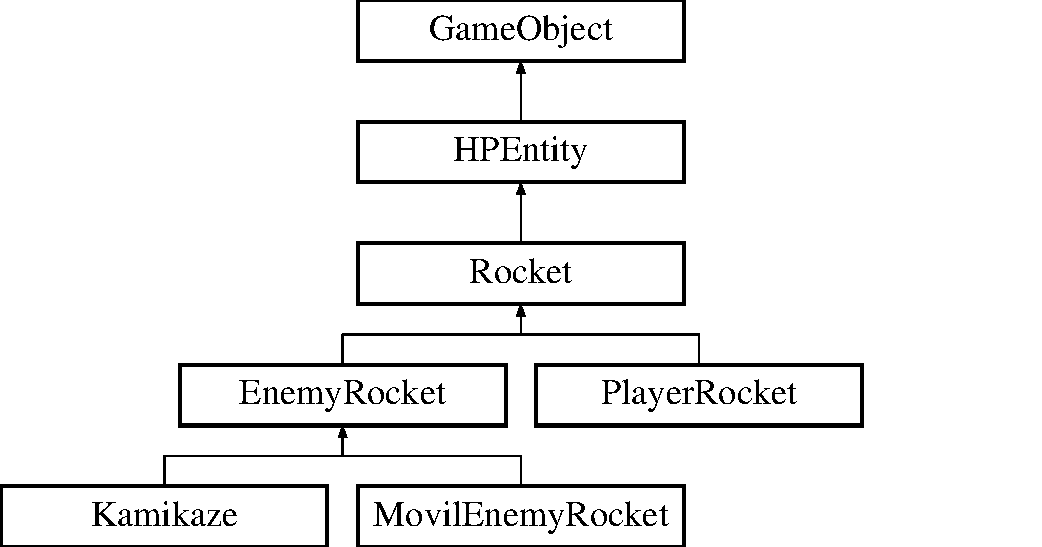
\includegraphics[height=5.000000cm]{class_rocket}
\end{center}
\end{figure}
\subsection*{Public Member Functions}
\begin{DoxyCompactItemize}
\item 
\hyperlink{class_rocket_a1414d17ed74b1da2c082f7f273bf55ab}{Rocket} (Q\-Rect p\-Rectangle, int p\-Max\-Hp)
\item 
void \hyperlink{class_rocket_aa0f4dcf673358e841e4b4b2fa0b1462e}{update} ()
\begin{DoxyCompactList}\small\item\em Actualiza el objeto, es un metodo abstracto, y debe ser implementado por sus clases hijas. \end{DoxyCompactList}\item 
void \hyperlink{class_rocket_ab381b27dd79eee5817dd61e46accd512}{set\-X\-Velocity} (int p\-X\-Velocity)
\item 
void \hyperlink{class_rocket_a27e02e296aeff2b15b3bc0f09c0c6b1c}{set\-Y\-Velocity} (int p\-Y\-Velocity)
\item 
int \hyperlink{class_rocket_a326aa42ccf341047a3009382e81eef7d}{get\-X\-Velocity} () const 
\item 
int \hyperlink{class_rocket_a981cf7e9bdf4f48adcf987f9a97d09e8}{get\-Y\-Velocity} () const 
\item 
virtual \hyperlink{class_shot}{Shot} $\ast$ \hyperlink{class_rocket_a5164f5926f96291b57da2516d46262e8}{shoot} ()=0
\item 
virtual \hyperlink{class_rocket_ab0cbe044146250c3e592832bb4909ff9}{$\sim$\-Rocket} ()
\end{DoxyCompactItemize}
\subsection*{Static Public Attributes}
\begin{DoxyCompactItemize}
\item 
static const int \hyperlink{class_rocket_ac8b2266f7e3aa777aca1b0144722a0db}{R\-O\-C\-K\-E\-T\-\_\-\-W\-I\-D\-T\-H} = 128
\item 
static const int \hyperlink{class_rocket_a5096c34316cb2b6116b3971f0cbb56f2}{R\-O\-C\-K\-E\-T\-\_\-\-H\-E\-I\-G\-H\-T} = 108
\item 
static const int \hyperlink{class_rocket_ad631a51a51c3dcbb927604c6b498498d}{M\-A\-X\-\_\-\-H\-P} = 100
\item 
static const int \hyperlink{class_rocket_adf93733f7bd7643acfb98d5e9feab7c5}{E\-N\-E\-M\-Y\-\_\-\-M\-A\-X\-\_\-\-H\-P} = 50
\item 
static const int \hyperlink{class_rocket_a1a590b76e2cc310e566f2624265f5c47}{R\-O\-C\-K\-E\-T\-\_\-\-V\-E\-L\-O\-C\-I\-T\-Y} = 15
\end{DoxyCompactItemize}
\subsection*{Protected Attributes}
\begin{DoxyCompactItemize}
\item 
int \hyperlink{class_rocket_af29030dcde63c0c11f394855eabeb035}{\-\_\-\-Vx}
\item 
int \hyperlink{class_rocket_a8755419e9cbd841f0ca08e9203d5d51b}{\-\_\-\-Vy}
\end{DoxyCompactItemize}
\subsection*{Additional Inherited Members}


\subsection{Constructor \& Destructor Documentation}
\hypertarget{class_rocket_a1414d17ed74b1da2c082f7f273bf55ab}{\index{Rocket@{Rocket}!Rocket@{Rocket}}
\index{Rocket@{Rocket}!Rocket@{Rocket}}
\subsubsection[{Rocket}]{\setlength{\rightskip}{0pt plus 5cm}Rocket\-::\-Rocket (
\begin{DoxyParamCaption}
\item[{Q\-Rect}]{p\-Rectangle, }
\item[{int}]{p\-Max\-Hp}
\end{DoxyParamCaption}
)}}\label{class_rocket_a1414d17ed74b1da2c082f7f273bf55ab}
\hypertarget{class_rocket_ab0cbe044146250c3e592832bb4909ff9}{\index{Rocket@{Rocket}!$\sim$\-Rocket@{$\sim$\-Rocket}}
\index{$\sim$\-Rocket@{$\sim$\-Rocket}!Rocket@{Rocket}}
\subsubsection[{$\sim$\-Rocket}]{\setlength{\rightskip}{0pt plus 5cm}Rocket\-::$\sim$\-Rocket (
\begin{DoxyParamCaption}
{}
\end{DoxyParamCaption}
)\hspace{0.3cm}{\ttfamily [virtual]}}}\label{class_rocket_ab0cbe044146250c3e592832bb4909ff9}


\subsection{Member Function Documentation}
\hypertarget{class_rocket_a326aa42ccf341047a3009382e81eef7d}{\index{Rocket@{Rocket}!get\-X\-Velocity@{get\-X\-Velocity}}
\index{get\-X\-Velocity@{get\-X\-Velocity}!Rocket@{Rocket}}
\subsubsection[{get\-X\-Velocity}]{\setlength{\rightskip}{0pt plus 5cm}int Rocket\-::get\-X\-Velocity (
\begin{DoxyParamCaption}
{}
\end{DoxyParamCaption}
) const}}\label{class_rocket_a326aa42ccf341047a3009382e81eef7d}
\hypertarget{class_rocket_a981cf7e9bdf4f48adcf987f9a97d09e8}{\index{Rocket@{Rocket}!get\-Y\-Velocity@{get\-Y\-Velocity}}
\index{get\-Y\-Velocity@{get\-Y\-Velocity}!Rocket@{Rocket}}
\subsubsection[{get\-Y\-Velocity}]{\setlength{\rightskip}{0pt plus 5cm}int Rocket\-::get\-Y\-Velocity (
\begin{DoxyParamCaption}
{}
\end{DoxyParamCaption}
) const}}\label{class_rocket_a981cf7e9bdf4f48adcf987f9a97d09e8}
\hypertarget{class_rocket_ab381b27dd79eee5817dd61e46accd512}{\index{Rocket@{Rocket}!set\-X\-Velocity@{set\-X\-Velocity}}
\index{set\-X\-Velocity@{set\-X\-Velocity}!Rocket@{Rocket}}
\subsubsection[{set\-X\-Velocity}]{\setlength{\rightskip}{0pt plus 5cm}void Rocket\-::set\-X\-Velocity (
\begin{DoxyParamCaption}
\item[{int}]{p\-X\-Velocity}
\end{DoxyParamCaption}
)}}\label{class_rocket_ab381b27dd79eee5817dd61e46accd512}
\hypertarget{class_rocket_a27e02e296aeff2b15b3bc0f09c0c6b1c}{\index{Rocket@{Rocket}!set\-Y\-Velocity@{set\-Y\-Velocity}}
\index{set\-Y\-Velocity@{set\-Y\-Velocity}!Rocket@{Rocket}}
\subsubsection[{set\-Y\-Velocity}]{\setlength{\rightskip}{0pt plus 5cm}void Rocket\-::set\-Y\-Velocity (
\begin{DoxyParamCaption}
\item[{int}]{p\-Y\-Velocity}
\end{DoxyParamCaption}
)}}\label{class_rocket_a27e02e296aeff2b15b3bc0f09c0c6b1c}
\hypertarget{class_rocket_a5164f5926f96291b57da2516d46262e8}{\index{Rocket@{Rocket}!shoot@{shoot}}
\index{shoot@{shoot}!Rocket@{Rocket}}
\subsubsection[{shoot}]{\setlength{\rightskip}{0pt plus 5cm}virtual {\bf Shot}$\ast$ Rocket\-::shoot (
\begin{DoxyParamCaption}
{}
\end{DoxyParamCaption}
)\hspace{0.3cm}{\ttfamily [pure virtual]}}}\label{class_rocket_a5164f5926f96291b57da2516d46262e8}


Implemented in \hyperlink{class_player_rocket_a1277f01884b2b1a68e312228e916805a}{Player\-Rocket}, and \hyperlink{class_enemy_rocket_aaa119ae66d24f37445ee53f0e2184bc2}{Enemy\-Rocket}.

\hypertarget{class_rocket_aa0f4dcf673358e841e4b4b2fa0b1462e}{\index{Rocket@{Rocket}!update@{update}}
\index{update@{update}!Rocket@{Rocket}}
\subsubsection[{update}]{\setlength{\rightskip}{0pt plus 5cm}void Rocket\-::update (
\begin{DoxyParamCaption}
{}
\end{DoxyParamCaption}
)\hspace{0.3cm}{\ttfamily [virtual]}}}\label{class_rocket_aa0f4dcf673358e841e4b4b2fa0b1462e}


Actualiza el objeto, es un metodo abstracto, y debe ser implementado por sus clases hijas. 



Implements \hyperlink{class_game_object_ae83128d0e0efef691417779605ee037c}{Game\-Object}.



\subsection{Member Data Documentation}
\hypertarget{class_rocket_af29030dcde63c0c11f394855eabeb035}{\index{Rocket@{Rocket}!\-\_\-\-Vx@{\-\_\-\-Vx}}
\index{\-\_\-\-Vx@{\-\_\-\-Vx}!Rocket@{Rocket}}
\subsubsection[{\-\_\-\-Vx}]{\setlength{\rightskip}{0pt plus 5cm}int Rocket\-::\-\_\-\-Vx\hspace{0.3cm}{\ttfamily [protected]}}}\label{class_rocket_af29030dcde63c0c11f394855eabeb035}
\hypertarget{class_rocket_a8755419e9cbd841f0ca08e9203d5d51b}{\index{Rocket@{Rocket}!\-\_\-\-Vy@{\-\_\-\-Vy}}
\index{\-\_\-\-Vy@{\-\_\-\-Vy}!Rocket@{Rocket}}
\subsubsection[{\-\_\-\-Vy}]{\setlength{\rightskip}{0pt plus 5cm}int Rocket\-::\-\_\-\-Vy\hspace{0.3cm}{\ttfamily [protected]}}}\label{class_rocket_a8755419e9cbd841f0ca08e9203d5d51b}
\hypertarget{class_rocket_adf93733f7bd7643acfb98d5e9feab7c5}{\index{Rocket@{Rocket}!E\-N\-E\-M\-Y\-\_\-\-M\-A\-X\-\_\-\-H\-P@{E\-N\-E\-M\-Y\-\_\-\-M\-A\-X\-\_\-\-H\-P}}
\index{E\-N\-E\-M\-Y\-\_\-\-M\-A\-X\-\_\-\-H\-P@{E\-N\-E\-M\-Y\-\_\-\-M\-A\-X\-\_\-\-H\-P}!Rocket@{Rocket}}
\subsubsection[{E\-N\-E\-M\-Y\-\_\-\-M\-A\-X\-\_\-\-H\-P}]{\setlength{\rightskip}{0pt plus 5cm}const int Rocket\-::\-E\-N\-E\-M\-Y\-\_\-\-M\-A\-X\-\_\-\-H\-P = 50\hspace{0.3cm}{\ttfamily [static]}}}\label{class_rocket_adf93733f7bd7643acfb98d5e9feab7c5}
\hypertarget{class_rocket_ad631a51a51c3dcbb927604c6b498498d}{\index{Rocket@{Rocket}!M\-A\-X\-\_\-\-H\-P@{M\-A\-X\-\_\-\-H\-P}}
\index{M\-A\-X\-\_\-\-H\-P@{M\-A\-X\-\_\-\-H\-P}!Rocket@{Rocket}}
\subsubsection[{M\-A\-X\-\_\-\-H\-P}]{\setlength{\rightskip}{0pt plus 5cm}const int Rocket\-::\-M\-A\-X\-\_\-\-H\-P = 100\hspace{0.3cm}{\ttfamily [static]}}}\label{class_rocket_ad631a51a51c3dcbb927604c6b498498d}
\hypertarget{class_rocket_a5096c34316cb2b6116b3971f0cbb56f2}{\index{Rocket@{Rocket}!R\-O\-C\-K\-E\-T\-\_\-\-H\-E\-I\-G\-H\-T@{R\-O\-C\-K\-E\-T\-\_\-\-H\-E\-I\-G\-H\-T}}
\index{R\-O\-C\-K\-E\-T\-\_\-\-H\-E\-I\-G\-H\-T@{R\-O\-C\-K\-E\-T\-\_\-\-H\-E\-I\-G\-H\-T}!Rocket@{Rocket}}
\subsubsection[{R\-O\-C\-K\-E\-T\-\_\-\-H\-E\-I\-G\-H\-T}]{\setlength{\rightskip}{0pt plus 5cm}const int Rocket\-::\-R\-O\-C\-K\-E\-T\-\_\-\-H\-E\-I\-G\-H\-T = 108\hspace{0.3cm}{\ttfamily [static]}}}\label{class_rocket_a5096c34316cb2b6116b3971f0cbb56f2}
\hypertarget{class_rocket_a1a590b76e2cc310e566f2624265f5c47}{\index{Rocket@{Rocket}!R\-O\-C\-K\-E\-T\-\_\-\-V\-E\-L\-O\-C\-I\-T\-Y@{R\-O\-C\-K\-E\-T\-\_\-\-V\-E\-L\-O\-C\-I\-T\-Y}}
\index{R\-O\-C\-K\-E\-T\-\_\-\-V\-E\-L\-O\-C\-I\-T\-Y@{R\-O\-C\-K\-E\-T\-\_\-\-V\-E\-L\-O\-C\-I\-T\-Y}!Rocket@{Rocket}}
\subsubsection[{R\-O\-C\-K\-E\-T\-\_\-\-V\-E\-L\-O\-C\-I\-T\-Y}]{\setlength{\rightskip}{0pt plus 5cm}const int Rocket\-::\-R\-O\-C\-K\-E\-T\-\_\-\-V\-E\-L\-O\-C\-I\-T\-Y = 15\hspace{0.3cm}{\ttfamily [static]}}}\label{class_rocket_a1a590b76e2cc310e566f2624265f5c47}
\hypertarget{class_rocket_ac8b2266f7e3aa777aca1b0144722a0db}{\index{Rocket@{Rocket}!R\-O\-C\-K\-E\-T\-\_\-\-W\-I\-D\-T\-H@{R\-O\-C\-K\-E\-T\-\_\-\-W\-I\-D\-T\-H}}
\index{R\-O\-C\-K\-E\-T\-\_\-\-W\-I\-D\-T\-H@{R\-O\-C\-K\-E\-T\-\_\-\-W\-I\-D\-T\-H}!Rocket@{Rocket}}
\subsubsection[{R\-O\-C\-K\-E\-T\-\_\-\-W\-I\-D\-T\-H}]{\setlength{\rightskip}{0pt plus 5cm}const int Rocket\-::\-R\-O\-C\-K\-E\-T\-\_\-\-W\-I\-D\-T\-H = 128\hspace{0.3cm}{\ttfamily [static]}}}\label{class_rocket_ac8b2266f7e3aa777aca1b0144722a0db}


The documentation for this class was generated from the following files\-:\begin{DoxyCompactItemize}
\item 
logic/rocket/\hyperlink{rocket_8h}{rocket.\-h}\item 
logic/rocket/\hyperlink{rocket_8cpp}{rocket.\-cpp}\end{DoxyCompactItemize}

\hypertarget{class_select_map}{\section{Select\-Map Class Reference}
\label{class_select_map}\index{Select\-Map@{Select\-Map}}
}
Inheritance diagram for Select\-Map\-:\begin{figure}[H]
\begin{center}
\leavevmode
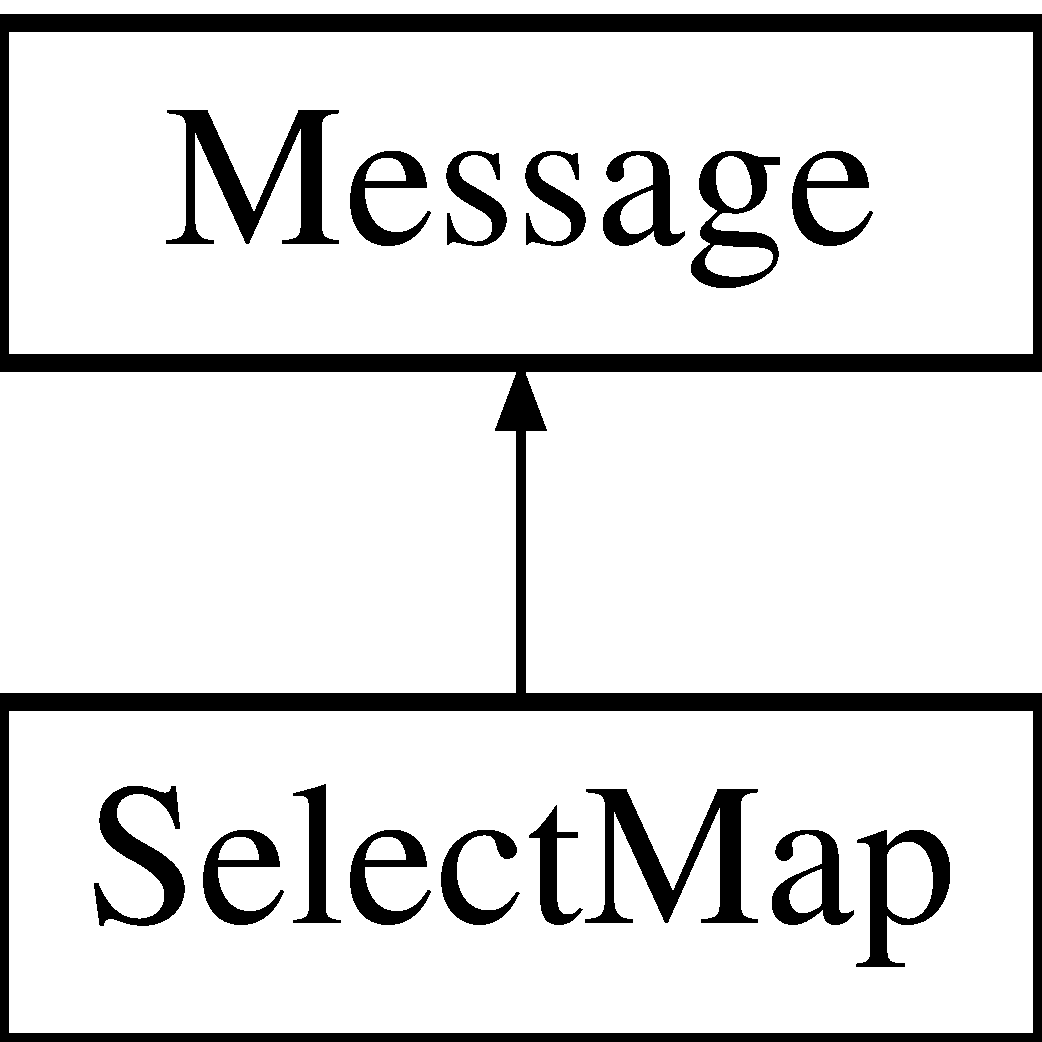
\includegraphics[height=2.000000cm]{class_select_map}
\end{center}
\end{figure}
\subsection*{Public Member Functions}
\begin{DoxyCompactItemize}
\item 
\hypertarget{class_select_map_afd9bc662490deae5232f13cfe8d4d9c8}{{\bfseries Select\-Map} (const \hyperlink{class_select_map}{Select\-Map} \&from)}\label{class_select_map_afd9bc662490deae5232f13cfe8d4d9c8}

\item 
\hypertarget{class_select_map_a3fd80cd851c3d73a7a5fa5dfb7babb24}{\hyperlink{class_select_map}{Select\-Map} \& {\bfseries operator=} (const \hyperlink{class_select_map}{Select\-Map} \&from)}\label{class_select_map_a3fd80cd851c3d73a7a5fa5dfb7babb24}

\item 
\hypertarget{class_select_map_ac90998108757f6fe2e476840d7fa5ec7}{const \\*
\-::google\-::protobuf\-::\-Unknown\-Field\-Set \& {\bfseries unknown\-\_\-fields} () const }\label{class_select_map_ac90998108757f6fe2e476840d7fa5ec7}

\item 
\hypertarget{class_select_map_ae89a46b8b228f94ebfa4fdd8f5496a7e}{inline\-::google\-::protobuf\-::\-Unknown\-Field\-Set $\ast$ {\bfseries mutable\-\_\-unknown\-\_\-fields} ()}\label{class_select_map_ae89a46b8b228f94ebfa4fdd8f5496a7e}

\item 
\hypertarget{class_select_map_a03757f1100f5af311c7eff655204af8c}{void {\bfseries Swap} (\hyperlink{class_select_map}{Select\-Map} $\ast$other)}\label{class_select_map_a03757f1100f5af311c7eff655204af8c}

\item 
\hypertarget{class_select_map_ac0bab665ca3c3cf9d86d6fdb0dd0db6d}{\hyperlink{class_select_map}{Select\-Map} $\ast$ {\bfseries New} () const }\label{class_select_map_ac0bab665ca3c3cf9d86d6fdb0dd0db6d}

\item 
\hypertarget{class_select_map_a489354efbe2a4c1098a2d02ac2a2a0d2}{\hyperlink{class_select_map}{Select\-Map} $\ast$ {\bfseries New} (\-::google\-::protobuf\-::\-Arena $\ast$arena) const }\label{class_select_map_a489354efbe2a4c1098a2d02ac2a2a0d2}

\item 
\hypertarget{class_select_map_a63de092351e6415542de23769886fbea}{void {\bfseries Copy\-From} (const \-::google\-::protobuf\-::\-Message \&from)}\label{class_select_map_a63de092351e6415542de23769886fbea}

\item 
\hypertarget{class_select_map_aa8fb7854b32ca284e6eb9a95990d04a8}{void {\bfseries Merge\-From} (const \-::google\-::protobuf\-::\-Message \&from)}\label{class_select_map_aa8fb7854b32ca284e6eb9a95990d04a8}

\item 
\hypertarget{class_select_map_abd53ee958264d56ea93505f1998ff85a}{void {\bfseries Copy\-From} (const \hyperlink{class_select_map}{Select\-Map} \&from)}\label{class_select_map_abd53ee958264d56ea93505f1998ff85a}

\item 
\hypertarget{class_select_map_a5a6cbf4a40503eb8b2f31c8a81fd2926}{void {\bfseries Merge\-From} (const \hyperlink{class_select_map}{Select\-Map} \&from)}\label{class_select_map_a5a6cbf4a40503eb8b2f31c8a81fd2926}

\item 
\hypertarget{class_select_map_a6c74d9780a2f9f3e025ad300bf9f8040}{void {\bfseries Clear} ()}\label{class_select_map_a6c74d9780a2f9f3e025ad300bf9f8040}

\item 
\hypertarget{class_select_map_a32ef5cff913db1dff34677313d8fca17}{bool {\bfseries Is\-Initialized} () const }\label{class_select_map_a32ef5cff913db1dff34677313d8fca17}

\item 
\hypertarget{class_select_map_a896f4de61429d66f7ca721665252540f}{int {\bfseries Byte\-Size} () const }\label{class_select_map_a896f4de61429d66f7ca721665252540f}

\item 
\hypertarget{class_select_map_ad1efa76b6521f8ec525aa955d4f8cbec}{bool {\bfseries Merge\-Partial\-From\-Coded\-Stream} (\-::google\-::protobuf\-::io\-::\-Coded\-Input\-Stream $\ast$input)}\label{class_select_map_ad1efa76b6521f8ec525aa955d4f8cbec}

\item 
\hypertarget{class_select_map_ad97d14500a1bfbe5d7d762c3a37796c7}{void {\bfseries Serialize\-With\-Cached\-Sizes} (\-::google\-::protobuf\-::io\-::\-Coded\-Output\-Stream $\ast$output) const }\label{class_select_map_ad97d14500a1bfbe5d7d762c3a37796c7}

\item 
\hypertarget{class_select_map_a7d09c9ffc748072867a1014e3c781292}{\-::google\-::protobuf\-::uint8 $\ast$ {\bfseries Serialize\-With\-Cached\-Sizes\-To\-Array} (\-::google\-::protobuf\-::uint8 $\ast$output) const }\label{class_select_map_a7d09c9ffc748072867a1014e3c781292}

\item 
\hypertarget{class_select_map_aa228e910522dc2fc1b80e28c3f1fe05c}{int {\bfseries Get\-Cached\-Size} () const }\label{class_select_map_aa228e910522dc2fc1b80e28c3f1fe05c}

\item 
\hypertarget{class_select_map_a6f0e3f4a17b808cfa28f50b761a832dd}{\-::google\-::protobuf\-::\-Metadata {\bfseries Get\-Metadata} () const }\label{class_select_map_a6f0e3f4a17b808cfa28f50b761a832dd}

\item 
\hypertarget{class_select_map_acbee86909008218756c875291f41a24c}{bool {\bfseries has\-\_\-numofmap} () const }\label{class_select_map_acbee86909008218756c875291f41a24c}

\item 
\hypertarget{class_select_map_ac7edf514f8e7f66dcc5d8bfbc586cad1}{void {\bfseries clear\-\_\-numofmap} ()}\label{class_select_map_ac7edf514f8e7f66dcc5d8bfbc586cad1}

\item 
\hypertarget{class_select_map_a68740fcce2df53fa898d0703cf7d33a7}{inline\-::google\-::protobuf\-::int32 {\bfseries numofmap} () const }\label{class_select_map_a68740fcce2df53fa898d0703cf7d33a7}

\item 
\hypertarget{class_select_map_aee810901a8840191d4b39ec7d53cb9cb}{void {\bfseries set\-\_\-numofmap} (\-::google\-::protobuf\-::int32 value)}\label{class_select_map_aee810901a8840191d4b39ec7d53cb9cb}

\end{DoxyCompactItemize}
\subsection*{Static Public Member Functions}
\begin{DoxyCompactItemize}
\item 
\hypertarget{class_select_map_a58714ef601b494a6f7b53446fd7ae3c4}{static const \\*
\-::google\-::protobuf\-::\-Descriptor $\ast$ {\bfseries descriptor} ()}\label{class_select_map_a58714ef601b494a6f7b53446fd7ae3c4}

\item 
\hypertarget{class_select_map_a33c33429463ad7c416b16e6af042c791}{static const \hyperlink{class_select_map}{Select\-Map} \& {\bfseries default\-\_\-instance} ()}\label{class_select_map_a33c33429463ad7c416b16e6af042c791}

\end{DoxyCompactItemize}
\subsection*{Static Public Attributes}
\begin{DoxyCompactItemize}
\item 
\hypertarget{class_select_map_a82d1599ce39896be4446fdc47fd087b4}{static const int {\bfseries k\-Num\-Of\-Map\-Field\-Number} = 1}\label{class_select_map_a82d1599ce39896be4446fdc47fd087b4}

\end{DoxyCompactItemize}
\subsection*{Friends}
\begin{DoxyCompactItemize}
\item 
\hypertarget{class_select_map_aad2611d2dc5aa84e66de3ab9abaa4b62}{void {\bfseries protobuf\-\_\-\-Add\-Desc\-\_\-\-Select\-Map\-\_\-2eproto} ()}\label{class_select_map_aad2611d2dc5aa84e66de3ab9abaa4b62}

\item 
\hypertarget{class_select_map_af70cd852226b57cecb6d29ffbb5455af}{void {\bfseries protobuf\-\_\-\-Assign\-Desc\-\_\-\-Select\-Map\-\_\-2eproto} ()}\label{class_select_map_af70cd852226b57cecb6d29ffbb5455af}

\item 
\hypertarget{class_select_map_a84edfc241ea5eb06701606ff9426e996}{void {\bfseries protobuf\-\_\-\-Shutdown\-File\-\_\-\-Select\-Map\-\_\-2eproto} ()}\label{class_select_map_a84edfc241ea5eb06701606ff9426e996}

\end{DoxyCompactItemize}


The documentation for this class was generated from the following files\-:\begin{DoxyCompactItemize}
\item 
protobufmessage/Select\-Map.\-pb.\-h\item 
protobufmessage/Select\-Map.\-pb.\-cc\end{DoxyCompactItemize}

\hypertarget{class_server_socket}{\section{Server\-Socket Class Reference}
\label{class_server_socket}\index{Server\-Socket@{Server\-Socket}}
}


{\ttfamily \#include $<$serversocket.\-h$>$}

Inheritance diagram for Server\-Socket\-:\begin{figure}[H]
\begin{center}
\leavevmode
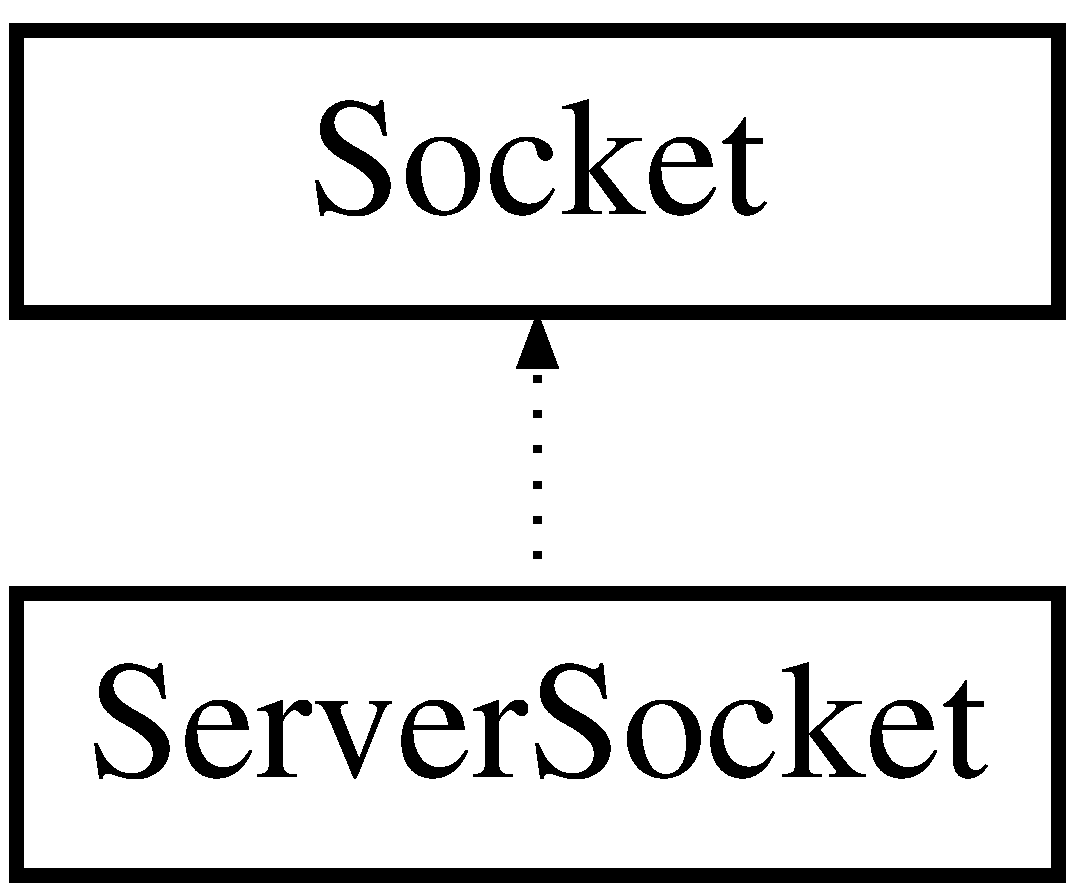
\includegraphics[height=2.000000cm]{class_server_socket}
\end{center}
\end{figure}
\subsection*{Public Member Functions}
\begin{DoxyCompactItemize}
\item 
\hyperlink{class_server_socket_a3dc1a31f740e4a8d69ae10c5dcb547d6}{Server\-Socket} (int port)
\item 
\hyperlink{class_server_socket_a2b3098589541243241ca25495155186c}{Server\-Socket} ()
\item 
virtual \hyperlink{class_server_socket_a510674d924c2544e6b0069e39c36516b}{$\sim$\-Server\-Socket} ()
\item 
const \hyperlink{class_server_socket}{Server\-Socket} \& \hyperlink{class_server_socket_ab5fe4b2d92d7014f7663c1bbacbbeda5}{operator$<$$<$} (const std\-::string \&) const 
\item 
const \hyperlink{class_server_socket}{Server\-Socket} \& \hyperlink{class_server_socket_a6bfabf01766bdb2c7f53274d8d771212}{operator$>$$>$} (std\-::string \&) const 
\item 
void \hyperlink{class_server_socket_ae550e314a988575d05b1dec1c3c18020}{accept} (\hyperlink{class_server_socket}{Server\-Socket} \&)
\end{DoxyCompactItemize}


\subsection{Constructor \& Destructor Documentation}
\hypertarget{class_server_socket_a3dc1a31f740e4a8d69ae10c5dcb547d6}{\index{Server\-Socket@{Server\-Socket}!Server\-Socket@{Server\-Socket}}
\index{Server\-Socket@{Server\-Socket}!ServerSocket@{Server\-Socket}}
\subsubsection[{Server\-Socket}]{\setlength{\rightskip}{0pt plus 5cm}Server\-Socket\-::\-Server\-Socket (
\begin{DoxyParamCaption}
\item[{int}]{port}
\end{DoxyParamCaption}
)}}\label{class_server_socket_a3dc1a31f740e4a8d69ae10c5dcb547d6}
\hypertarget{class_server_socket_a2b3098589541243241ca25495155186c}{\index{Server\-Socket@{Server\-Socket}!Server\-Socket@{Server\-Socket}}
\index{Server\-Socket@{Server\-Socket}!ServerSocket@{Server\-Socket}}
\subsubsection[{Server\-Socket}]{\setlength{\rightskip}{0pt plus 5cm}Server\-Socket\-::\-Server\-Socket (
\begin{DoxyParamCaption}
{}
\end{DoxyParamCaption}
)\hspace{0.3cm}{\ttfamily [inline]}}}\label{class_server_socket_a2b3098589541243241ca25495155186c}
\hypertarget{class_server_socket_a510674d924c2544e6b0069e39c36516b}{\index{Server\-Socket@{Server\-Socket}!$\sim$\-Server\-Socket@{$\sim$\-Server\-Socket}}
\index{$\sim$\-Server\-Socket@{$\sim$\-Server\-Socket}!ServerSocket@{Server\-Socket}}
\subsubsection[{$\sim$\-Server\-Socket}]{\setlength{\rightskip}{0pt plus 5cm}Server\-Socket\-::$\sim$\-Server\-Socket (
\begin{DoxyParamCaption}
{}
\end{DoxyParamCaption}
)\hspace{0.3cm}{\ttfamily [virtual]}}}\label{class_server_socket_a510674d924c2544e6b0069e39c36516b}


\subsection{Member Function Documentation}
\hypertarget{class_server_socket_ae550e314a988575d05b1dec1c3c18020}{\index{Server\-Socket@{Server\-Socket}!accept@{accept}}
\index{accept@{accept}!ServerSocket@{Server\-Socket}}
\subsubsection[{accept}]{\setlength{\rightskip}{0pt plus 5cm}void Server\-Socket\-::accept (
\begin{DoxyParamCaption}
\item[{{\bf Server\-Socket} \&}]{sock}
\end{DoxyParamCaption}
)}}\label{class_server_socket_ae550e314a988575d05b1dec1c3c18020}
\hypertarget{class_server_socket_ab5fe4b2d92d7014f7663c1bbacbbeda5}{\index{Server\-Socket@{Server\-Socket}!operator$<$$<$@{operator$<$$<$}}
\index{operator$<$$<$@{operator$<$$<$}!ServerSocket@{Server\-Socket}}
\subsubsection[{operator$<$$<$}]{\setlength{\rightskip}{0pt plus 5cm}const {\bf Server\-Socket} \& Server\-Socket\-::operator$<$$<$ (
\begin{DoxyParamCaption}
\item[{const std\-::string \&}]{s}
\end{DoxyParamCaption}
) const}}\label{class_server_socket_ab5fe4b2d92d7014f7663c1bbacbbeda5}
\hypertarget{class_server_socket_a6bfabf01766bdb2c7f53274d8d771212}{\index{Server\-Socket@{Server\-Socket}!operator$>$$>$@{operator$>$$>$}}
\index{operator$>$$>$@{operator$>$$>$}!ServerSocket@{Server\-Socket}}
\subsubsection[{operator$>$$>$}]{\setlength{\rightskip}{0pt plus 5cm}const {\bf Server\-Socket} \& Server\-Socket\-::operator$>$$>$ (
\begin{DoxyParamCaption}
\item[{std\-::string \&}]{s}
\end{DoxyParamCaption}
) const}}\label{class_server_socket_a6bfabf01766bdb2c7f53274d8d771212}


The documentation for this class was generated from the following files\-:\begin{DoxyCompactItemize}
\item 
logic/lanconection/\hyperlink{serversocket_8h}{serversocket.\-h}\item 
logic/lanconection/\hyperlink{serversocket_8cpp}{serversocket.\-cpp}\end{DoxyCompactItemize}

\hypertarget{class_shot}{\section{Shot Class Reference}
\label{class_shot}\index{Shot@{Shot}}
}


{\ttfamily \#include $<$shot.\-h$>$}

Inheritance diagram for Shot\-:\begin{figure}[H]
\begin{center}
\leavevmode
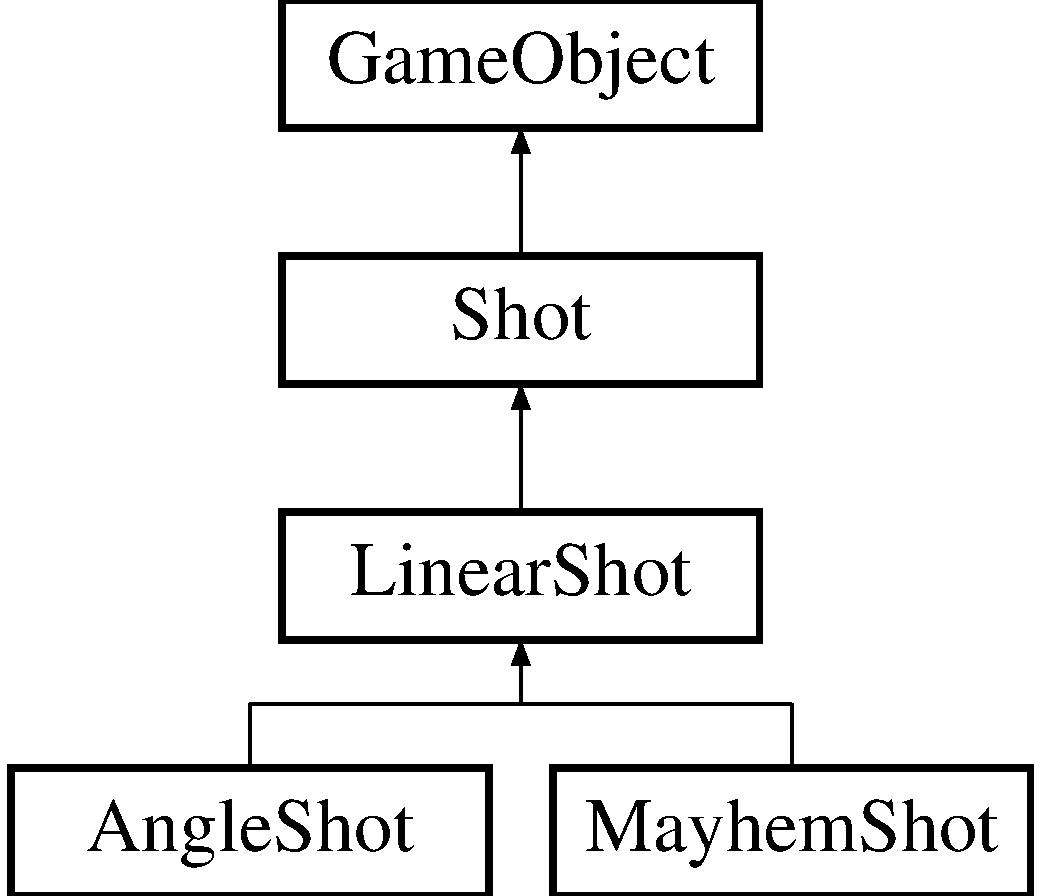
\includegraphics[height=4.000000cm]{class_shot}
\end{center}
\end{figure}
\subsection*{Public Member Functions}
\begin{DoxyCompactItemize}
\item 
\hyperlink{class_shot_a8fec158d22bc06cf7b8e4bc9c2328356}{Shot} (Q\-Rect p\-Rectangle, int p\-Damage)
\item 
virtual void \hyperlink{class_shot_a6f78a6d0f6e7e44619b0128c14ce5730}{damage} (\hyperlink{class_h_p_entity}{H\-P\-Entity} $\ast$p\-Entity)
\item 
virtual bool \hyperlink{class_shot_aa8acb047c32e567e066e75782744de62}{is\-Useful\-Shot} (Q\-Rect p\-Area)=0
\item 
virtual int \hyperlink{class_shot_a8cfb5cf554b6164f2dceef2e7263b8a0}{get\-X\-Velocity} ()=0
\item 
virtual int \hyperlink{class_shot_adad108f4ef3c792dc09eeb60a32d7479}{get\-Y\-Velocity} ()=0
\item 
virtual int \hyperlink{class_shot_a3bf2af64550a0ee1d467bdec43ac6200}{get\-Type} ()=0
\item 
virtual \hyperlink{class_shot_af090cf0eae5828befac25287e93b08f1}{$\sim$\-Shot} ()
\end{DoxyCompactItemize}
\subsection*{Static Public Attributes}
\begin{DoxyCompactItemize}
\item 
static const int \hyperlink{class_shot_af9fdec8f5ede1faa442fac378a81b072}{V\-E\-L\-O\-C\-I\-T\-Y} = 20
\item 
static const int \hyperlink{class_shot_a26d13b7f383ca64bb6e775b8dbaba834}{A\-N\-G\-L\-E\-\_\-\-S\-H\-O\-T} = 2
\item 
static const int \hyperlink{class_shot_a5b86e410ce75a9e9c5277e6a3a6ebbf7}{L\-I\-N\-E\-A\-R\-\_\-\-S\-H\-O\-T} = 1
\item 
static const int \hyperlink{class_shot_aea2978e9d7f2212f66d33b44fa864e7c}{M\-A\-Y\-H\-E\-M\-\_\-\-S\-H\-O\-T} = 3
\item 
static const int \hyperlink{class_shot_a8b4df95b379ba5fbecc41612c086f429}{W\-I\-D\-T\-H\-\_\-\-S\-H\-O\-T} = 32
\item 
static const int \hyperlink{class_shot_a1f4c11429e906bd99576ed89dcc1c487}{H\-E\-I\-G\-H\-T\-\_\-\-S\-H\-O\-T} = 32
\item 
static const int \hyperlink{class_shot_a1f093fa878e873dd07133df7217c0298}{E\-N\-E\-M\-Y\-\_\-\-D\-A\-M\-A\-G\-E} = -\/5
\item 
static const int \hyperlink{class_shot_a2c364fcd4dec0d1e0f4b2df259df80c5}{M\-A\-Y\-H\-E\-M\-\_\-\-D\-A\-M\-A\-G\-E} = -\/800
\item 
static const int \hyperlink{class_shot_a795b718149dd6d1ab4162103bd0a31c9}{A\-N\-G\-U\-L\-A\-R\-\_\-\-D\-A\-M\-A\-G\-E} = -\/8
\item 
static const int \hyperlink{class_shot_a678ee4d5bb816dc0e0ece5f88e887ec3}{L\-I\-N\-E\-A\-R\-\_\-\-D\-A\-M\-A\-G\-E} = -\/8
\item 
static const bool \hyperlink{class_shot_a578cf779712b5b7752c3d900c062f49c}{S\-H\-O\-T\-\_\-\-T\-O\-\_\-\-U\-P} = true
\item 
static const bool \hyperlink{class_shot_a1e552f6e2ad653bf2b1313f870566a17}{S\-H\-O\-T\-\_\-\-T\-O\-\_\-\-D\-O\-W\-N} = false
\end{DoxyCompactItemize}
\subsection*{Protected Attributes}
\begin{DoxyCompactItemize}
\item 
int \hyperlink{class_shot_a1aa9cf447026ba338930899bebde1d4b}{\-\_\-\-Damage}
\end{DoxyCompactItemize}
\subsection*{Additional Inherited Members}


\subsection{Constructor \& Destructor Documentation}
\hypertarget{class_shot_a8fec158d22bc06cf7b8e4bc9c2328356}{\index{Shot@{Shot}!Shot@{Shot}}
\index{Shot@{Shot}!Shot@{Shot}}
\subsubsection[{Shot}]{\setlength{\rightskip}{0pt plus 5cm}Shot\-::\-Shot (
\begin{DoxyParamCaption}
\item[{Q\-Rect}]{p\-Rectangle, }
\item[{int}]{p\-Damage}
\end{DoxyParamCaption}
)}}\label{class_shot_a8fec158d22bc06cf7b8e4bc9c2328356}
\hypertarget{class_shot_af090cf0eae5828befac25287e93b08f1}{\index{Shot@{Shot}!$\sim$\-Shot@{$\sim$\-Shot}}
\index{$\sim$\-Shot@{$\sim$\-Shot}!Shot@{Shot}}
\subsubsection[{$\sim$\-Shot}]{\setlength{\rightskip}{0pt plus 5cm}virtual Shot\-::$\sim$\-Shot (
\begin{DoxyParamCaption}
{}
\end{DoxyParamCaption}
)\hspace{0.3cm}{\ttfamily [inline]}, {\ttfamily [virtual]}}}\label{class_shot_af090cf0eae5828befac25287e93b08f1}


\subsection{Member Function Documentation}
\hypertarget{class_shot_a6f78a6d0f6e7e44619b0128c14ce5730}{\index{Shot@{Shot}!damage@{damage}}
\index{damage@{damage}!Shot@{Shot}}
\subsubsection[{damage}]{\setlength{\rightskip}{0pt plus 5cm}void Shot\-::damage (
\begin{DoxyParamCaption}
\item[{{\bf H\-P\-Entity} $\ast$}]{p\-Entity}
\end{DoxyParamCaption}
)\hspace{0.3cm}{\ttfamily [virtual]}}}\label{class_shot_a6f78a6d0f6e7e44619b0128c14ce5730}


Reimplemented in \hyperlink{class_mayhem_shot_aae8e9c0bcac2eddc50774decf0fd7c2e}{Mayhem\-Shot}.

\hypertarget{class_shot_a3bf2af64550a0ee1d467bdec43ac6200}{\index{Shot@{Shot}!get\-Type@{get\-Type}}
\index{get\-Type@{get\-Type}!Shot@{Shot}}
\subsubsection[{get\-Type}]{\setlength{\rightskip}{0pt plus 5cm}virtual int Shot\-::get\-Type (
\begin{DoxyParamCaption}
{}
\end{DoxyParamCaption}
)\hspace{0.3cm}{\ttfamily [pure virtual]}}}\label{class_shot_a3bf2af64550a0ee1d467bdec43ac6200}


Implemented in \hyperlink{class_linear_shot_a50717d095ffb35f445f909f0ef961a5a}{Linear\-Shot}, \hyperlink{class_angle_shot_a690154e0ae49ac8667046f0c4a9c1647}{Angle\-Shot}, and \hyperlink{class_mayhem_shot_a2aa6e9bf2e931477ace1731d3eed0500}{Mayhem\-Shot}.

\hypertarget{class_shot_a8cfb5cf554b6164f2dceef2e7263b8a0}{\index{Shot@{Shot}!get\-X\-Velocity@{get\-X\-Velocity}}
\index{get\-X\-Velocity@{get\-X\-Velocity}!Shot@{Shot}}
\subsubsection[{get\-X\-Velocity}]{\setlength{\rightskip}{0pt plus 5cm}virtual int Shot\-::get\-X\-Velocity (
\begin{DoxyParamCaption}
{}
\end{DoxyParamCaption}
)\hspace{0.3cm}{\ttfamily [pure virtual]}}}\label{class_shot_a8cfb5cf554b6164f2dceef2e7263b8a0}


Implemented in \hyperlink{class_linear_shot_a9f7b9d654314185d6d89c8c24a64bc85}{Linear\-Shot}, and \hyperlink{class_angle_shot_a7e51f41031536ff1086055eab24d544d}{Angle\-Shot}.

\hypertarget{class_shot_adad108f4ef3c792dc09eeb60a32d7479}{\index{Shot@{Shot}!get\-Y\-Velocity@{get\-Y\-Velocity}}
\index{get\-Y\-Velocity@{get\-Y\-Velocity}!Shot@{Shot}}
\subsubsection[{get\-Y\-Velocity}]{\setlength{\rightskip}{0pt plus 5cm}virtual int Shot\-::get\-Y\-Velocity (
\begin{DoxyParamCaption}
{}
\end{DoxyParamCaption}
)\hspace{0.3cm}{\ttfamily [pure virtual]}}}\label{class_shot_adad108f4ef3c792dc09eeb60a32d7479}


Implemented in \hyperlink{class_linear_shot_ad0b2c8f2e67c4c8bf48895616c9f5683}{Linear\-Shot}.

\hypertarget{class_shot_aa8acb047c32e567e066e75782744de62}{\index{Shot@{Shot}!is\-Useful\-Shot@{is\-Useful\-Shot}}
\index{is\-Useful\-Shot@{is\-Useful\-Shot}!Shot@{Shot}}
\subsubsection[{is\-Useful\-Shot}]{\setlength{\rightskip}{0pt plus 5cm}virtual bool Shot\-::is\-Useful\-Shot (
\begin{DoxyParamCaption}
\item[{Q\-Rect}]{p\-Area}
\end{DoxyParamCaption}
)\hspace{0.3cm}{\ttfamily [pure virtual]}}}\label{class_shot_aa8acb047c32e567e066e75782744de62}


Implemented in \hyperlink{class_linear_shot_af5e24419776495f3b42381fe614a3bec}{Linear\-Shot}.



\subsection{Member Data Documentation}
\hypertarget{class_shot_a1aa9cf447026ba338930899bebde1d4b}{\index{Shot@{Shot}!\-\_\-\-Damage@{\-\_\-\-Damage}}
\index{\-\_\-\-Damage@{\-\_\-\-Damage}!Shot@{Shot}}
\subsubsection[{\-\_\-\-Damage}]{\setlength{\rightskip}{0pt plus 5cm}int Shot\-::\-\_\-\-Damage\hspace{0.3cm}{\ttfamily [protected]}}}\label{class_shot_a1aa9cf447026ba338930899bebde1d4b}
\hypertarget{class_shot_a26d13b7f383ca64bb6e775b8dbaba834}{\index{Shot@{Shot}!A\-N\-G\-L\-E\-\_\-\-S\-H\-O\-T@{A\-N\-G\-L\-E\-\_\-\-S\-H\-O\-T}}
\index{A\-N\-G\-L\-E\-\_\-\-S\-H\-O\-T@{A\-N\-G\-L\-E\-\_\-\-S\-H\-O\-T}!Shot@{Shot}}
\subsubsection[{A\-N\-G\-L\-E\-\_\-\-S\-H\-O\-T}]{\setlength{\rightskip}{0pt plus 5cm}const int Shot\-::\-A\-N\-G\-L\-E\-\_\-\-S\-H\-O\-T = 2\hspace{0.3cm}{\ttfamily [static]}}}\label{class_shot_a26d13b7f383ca64bb6e775b8dbaba834}
\hypertarget{class_shot_a795b718149dd6d1ab4162103bd0a31c9}{\index{Shot@{Shot}!A\-N\-G\-U\-L\-A\-R\-\_\-\-D\-A\-M\-A\-G\-E@{A\-N\-G\-U\-L\-A\-R\-\_\-\-D\-A\-M\-A\-G\-E}}
\index{A\-N\-G\-U\-L\-A\-R\-\_\-\-D\-A\-M\-A\-G\-E@{A\-N\-G\-U\-L\-A\-R\-\_\-\-D\-A\-M\-A\-G\-E}!Shot@{Shot}}
\subsubsection[{A\-N\-G\-U\-L\-A\-R\-\_\-\-D\-A\-M\-A\-G\-E}]{\setlength{\rightskip}{0pt plus 5cm}const int Shot\-::\-A\-N\-G\-U\-L\-A\-R\-\_\-\-D\-A\-M\-A\-G\-E = -\/8\hspace{0.3cm}{\ttfamily [static]}}}\label{class_shot_a795b718149dd6d1ab4162103bd0a31c9}
\hypertarget{class_shot_a1f093fa878e873dd07133df7217c0298}{\index{Shot@{Shot}!E\-N\-E\-M\-Y\-\_\-\-D\-A\-M\-A\-G\-E@{E\-N\-E\-M\-Y\-\_\-\-D\-A\-M\-A\-G\-E}}
\index{E\-N\-E\-M\-Y\-\_\-\-D\-A\-M\-A\-G\-E@{E\-N\-E\-M\-Y\-\_\-\-D\-A\-M\-A\-G\-E}!Shot@{Shot}}
\subsubsection[{E\-N\-E\-M\-Y\-\_\-\-D\-A\-M\-A\-G\-E}]{\setlength{\rightskip}{0pt plus 5cm}const int Shot\-::\-E\-N\-E\-M\-Y\-\_\-\-D\-A\-M\-A\-G\-E = -\/5\hspace{0.3cm}{\ttfamily [static]}}}\label{class_shot_a1f093fa878e873dd07133df7217c0298}
\hypertarget{class_shot_a1f4c11429e906bd99576ed89dcc1c487}{\index{Shot@{Shot}!H\-E\-I\-G\-H\-T\-\_\-\-S\-H\-O\-T@{H\-E\-I\-G\-H\-T\-\_\-\-S\-H\-O\-T}}
\index{H\-E\-I\-G\-H\-T\-\_\-\-S\-H\-O\-T@{H\-E\-I\-G\-H\-T\-\_\-\-S\-H\-O\-T}!Shot@{Shot}}
\subsubsection[{H\-E\-I\-G\-H\-T\-\_\-\-S\-H\-O\-T}]{\setlength{\rightskip}{0pt plus 5cm}const int Shot\-::\-H\-E\-I\-G\-H\-T\-\_\-\-S\-H\-O\-T = 32\hspace{0.3cm}{\ttfamily [static]}}}\label{class_shot_a1f4c11429e906bd99576ed89dcc1c487}
\hypertarget{class_shot_a678ee4d5bb816dc0e0ece5f88e887ec3}{\index{Shot@{Shot}!L\-I\-N\-E\-A\-R\-\_\-\-D\-A\-M\-A\-G\-E@{L\-I\-N\-E\-A\-R\-\_\-\-D\-A\-M\-A\-G\-E}}
\index{L\-I\-N\-E\-A\-R\-\_\-\-D\-A\-M\-A\-G\-E@{L\-I\-N\-E\-A\-R\-\_\-\-D\-A\-M\-A\-G\-E}!Shot@{Shot}}
\subsubsection[{L\-I\-N\-E\-A\-R\-\_\-\-D\-A\-M\-A\-G\-E}]{\setlength{\rightskip}{0pt plus 5cm}const int Shot\-::\-L\-I\-N\-E\-A\-R\-\_\-\-D\-A\-M\-A\-G\-E = -\/8\hspace{0.3cm}{\ttfamily [static]}}}\label{class_shot_a678ee4d5bb816dc0e0ece5f88e887ec3}
\hypertarget{class_shot_a5b86e410ce75a9e9c5277e6a3a6ebbf7}{\index{Shot@{Shot}!L\-I\-N\-E\-A\-R\-\_\-\-S\-H\-O\-T@{L\-I\-N\-E\-A\-R\-\_\-\-S\-H\-O\-T}}
\index{L\-I\-N\-E\-A\-R\-\_\-\-S\-H\-O\-T@{L\-I\-N\-E\-A\-R\-\_\-\-S\-H\-O\-T}!Shot@{Shot}}
\subsubsection[{L\-I\-N\-E\-A\-R\-\_\-\-S\-H\-O\-T}]{\setlength{\rightskip}{0pt plus 5cm}const int Shot\-::\-L\-I\-N\-E\-A\-R\-\_\-\-S\-H\-O\-T = 1\hspace{0.3cm}{\ttfamily [static]}}}\label{class_shot_a5b86e410ce75a9e9c5277e6a3a6ebbf7}
\hypertarget{class_shot_a2c364fcd4dec0d1e0f4b2df259df80c5}{\index{Shot@{Shot}!M\-A\-Y\-H\-E\-M\-\_\-\-D\-A\-M\-A\-G\-E@{M\-A\-Y\-H\-E\-M\-\_\-\-D\-A\-M\-A\-G\-E}}
\index{M\-A\-Y\-H\-E\-M\-\_\-\-D\-A\-M\-A\-G\-E@{M\-A\-Y\-H\-E\-M\-\_\-\-D\-A\-M\-A\-G\-E}!Shot@{Shot}}
\subsubsection[{M\-A\-Y\-H\-E\-M\-\_\-\-D\-A\-M\-A\-G\-E}]{\setlength{\rightskip}{0pt plus 5cm}const int Shot\-::\-M\-A\-Y\-H\-E\-M\-\_\-\-D\-A\-M\-A\-G\-E = -\/800\hspace{0.3cm}{\ttfamily [static]}}}\label{class_shot_a2c364fcd4dec0d1e0f4b2df259df80c5}
\hypertarget{class_shot_aea2978e9d7f2212f66d33b44fa864e7c}{\index{Shot@{Shot}!M\-A\-Y\-H\-E\-M\-\_\-\-S\-H\-O\-T@{M\-A\-Y\-H\-E\-M\-\_\-\-S\-H\-O\-T}}
\index{M\-A\-Y\-H\-E\-M\-\_\-\-S\-H\-O\-T@{M\-A\-Y\-H\-E\-M\-\_\-\-S\-H\-O\-T}!Shot@{Shot}}
\subsubsection[{M\-A\-Y\-H\-E\-M\-\_\-\-S\-H\-O\-T}]{\setlength{\rightskip}{0pt plus 5cm}const int Shot\-::\-M\-A\-Y\-H\-E\-M\-\_\-\-S\-H\-O\-T = 3\hspace{0.3cm}{\ttfamily [static]}}}\label{class_shot_aea2978e9d7f2212f66d33b44fa864e7c}
\hypertarget{class_shot_a1e552f6e2ad653bf2b1313f870566a17}{\index{Shot@{Shot}!S\-H\-O\-T\-\_\-\-T\-O\-\_\-\-D\-O\-W\-N@{S\-H\-O\-T\-\_\-\-T\-O\-\_\-\-D\-O\-W\-N}}
\index{S\-H\-O\-T\-\_\-\-T\-O\-\_\-\-D\-O\-W\-N@{S\-H\-O\-T\-\_\-\-T\-O\-\_\-\-D\-O\-W\-N}!Shot@{Shot}}
\subsubsection[{S\-H\-O\-T\-\_\-\-T\-O\-\_\-\-D\-O\-W\-N}]{\setlength{\rightskip}{0pt plus 5cm}const bool Shot\-::\-S\-H\-O\-T\-\_\-\-T\-O\-\_\-\-D\-O\-W\-N = false\hspace{0.3cm}{\ttfamily [static]}}}\label{class_shot_a1e552f6e2ad653bf2b1313f870566a17}
\hypertarget{class_shot_a578cf779712b5b7752c3d900c062f49c}{\index{Shot@{Shot}!S\-H\-O\-T\-\_\-\-T\-O\-\_\-\-U\-P@{S\-H\-O\-T\-\_\-\-T\-O\-\_\-\-U\-P}}
\index{S\-H\-O\-T\-\_\-\-T\-O\-\_\-\-U\-P@{S\-H\-O\-T\-\_\-\-T\-O\-\_\-\-U\-P}!Shot@{Shot}}
\subsubsection[{S\-H\-O\-T\-\_\-\-T\-O\-\_\-\-U\-P}]{\setlength{\rightskip}{0pt plus 5cm}const bool Shot\-::\-S\-H\-O\-T\-\_\-\-T\-O\-\_\-\-U\-P = true\hspace{0.3cm}{\ttfamily [static]}}}\label{class_shot_a578cf779712b5b7752c3d900c062f49c}
\hypertarget{class_shot_af9fdec8f5ede1faa442fac378a81b072}{\index{Shot@{Shot}!V\-E\-L\-O\-C\-I\-T\-Y@{V\-E\-L\-O\-C\-I\-T\-Y}}
\index{V\-E\-L\-O\-C\-I\-T\-Y@{V\-E\-L\-O\-C\-I\-T\-Y}!Shot@{Shot}}
\subsubsection[{V\-E\-L\-O\-C\-I\-T\-Y}]{\setlength{\rightskip}{0pt plus 5cm}const int Shot\-::\-V\-E\-L\-O\-C\-I\-T\-Y = 20\hspace{0.3cm}{\ttfamily [static]}}}\label{class_shot_af9fdec8f5ede1faa442fac378a81b072}
\hypertarget{class_shot_a8b4df95b379ba5fbecc41612c086f429}{\index{Shot@{Shot}!W\-I\-D\-T\-H\-\_\-\-S\-H\-O\-T@{W\-I\-D\-T\-H\-\_\-\-S\-H\-O\-T}}
\index{W\-I\-D\-T\-H\-\_\-\-S\-H\-O\-T@{W\-I\-D\-T\-H\-\_\-\-S\-H\-O\-T}!Shot@{Shot}}
\subsubsection[{W\-I\-D\-T\-H\-\_\-\-S\-H\-O\-T}]{\setlength{\rightskip}{0pt plus 5cm}const int Shot\-::\-W\-I\-D\-T\-H\-\_\-\-S\-H\-O\-T = 32\hspace{0.3cm}{\ttfamily [static]}}}\label{class_shot_a8b4df95b379ba5fbecc41612c086f429}


The documentation for this class was generated from the following files\-:\begin{DoxyCompactItemize}
\item 
logic/shot/\hyperlink{shot_8h}{shot.\-h}\item 
logic/shot/\hyperlink{shot_8cpp}{shot.\-cpp}\end{DoxyCompactItemize}

\hypertarget{class_shot_fabric}{\section{Shot\-Fabric Class Reference}
\label{class_shot_fabric}\index{Shot\-Fabric@{Shot\-Fabric}}
}
Inheritance diagram for Shot\-Fabric\-:\begin{figure}[H]
\begin{center}
\leavevmode
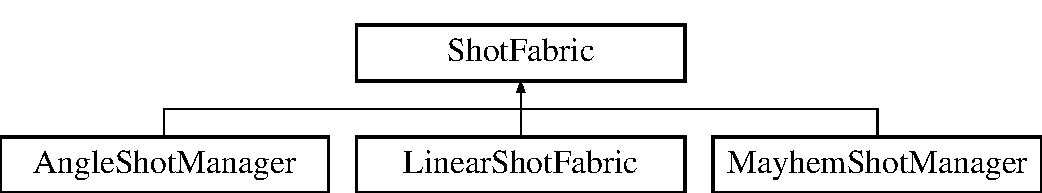
\includegraphics[height=2.000000cm]{class_shot_fabric}
\end{center}
\end{figure}
\subsection*{Public Member Functions}
\begin{DoxyCompactItemize}
\item 
\hypertarget{class_shot_fabric_af16f37a0f8bd2d7c92adc41af55d35fa}{{\bfseries Shot\-Fabric} (int p\-Max\-Munition)}\label{class_shot_fabric_af16f37a0f8bd2d7c92adc41af55d35fa}

\item 
\hypertarget{class_shot_fabric_a08f334290a4ef5dfd67964c35467344f}{virtual \hyperlink{class_shot}{Shot} $\ast$ {\bfseries get\-New\-Shoot} (int p\-X, int p\-Y, bool p\-Player)=0}\label{class_shot_fabric_a08f334290a4ef5dfd67964c35467344f}

\item 
\hypertarget{class_shot_fabric_a5cf24e648d9bb4dcafe30be3df7e64f8}{void {\bfseries add\-Munition} (int p\-Munition)}\label{class_shot_fabric_a5cf24e648d9bb4dcafe30be3df7e64f8}

\item 
\hypertarget{class_shot_fabric_a1f09703a48a7dc51c177dab863c14a17}{bool {\bfseries have\-Munition} ()}\label{class_shot_fabric_a1f09703a48a7dc51c177dab863c14a17}

\item 
\hypertarget{class_shot_fabric_a733c2e929d1ac1a30453e32af1874cbe}{int {\bfseries get\-Munitions} ()}\label{class_shot_fabric_a733c2e929d1ac1a30453e32af1874cbe}

\item 
\hypertarget{class_shot_fabric_a5744630f76e016e21ba141bd182d16ad}{virtual int {\bfseries get\-Munition\-Type} ()=0}\label{class_shot_fabric_a5744630f76e016e21ba141bd182d16ad}

\end{DoxyCompactItemize}
\subsection*{Protected Attributes}
\begin{DoxyCompactItemize}
\item 
\hypertarget{class_shot_fabric_a89ed1c6e673c23fa50018dd06d867a66}{int {\bfseries \-\_\-\-Max\-Munition}}\label{class_shot_fabric_a89ed1c6e673c23fa50018dd06d867a66}

\item 
\hypertarget{class_shot_fabric_a5863cbc4e51a089b3e87a1afd77629ba}{int {\bfseries \-\_\-\-Current\-Munition}}\label{class_shot_fabric_a5863cbc4e51a089b3e87a1afd77629ba}

\end{DoxyCompactItemize}


The documentation for this class was generated from the following files\-:\begin{DoxyCompactItemize}
\item 
logic/shot/shotfabric.\-h\item 
logic/shot/shotfabric.\-cpp\end{DoxyCompactItemize}

\hypertarget{class_shot_manager}{\section{Shot\-Manager Class Reference}
\label{class_shot_manager}\index{Shot\-Manager@{Shot\-Manager}}
}


{\ttfamily \#include $<$shotmanager.\-h$>$}

\subsection*{Public Member Functions}
\begin{DoxyCompactItemize}
\item 
\hyperlink{class_shot_manager_ab985b08b77a340ed984ed52e97aed7f9}{Shot\-Manager} ()
\item 
\hyperlink{class_shot}{Shot} $\ast$ \hyperlink{class_shot_manager_a9ffcd5b29ccba8b53308c5442c3cb13a}{create\-Munition} (int p\-X, int p\-Y)
\item 
void \hyperlink{class_shot_manager_aebd2c9ed59082d4382d367abd7b39dd5}{next\-Munition} ()
\item 
void \hyperlink{class_shot_manager_af5fe9ec898ebccb644e4fdaa679bb255}{add\-Munition} (int p\-Munition)
\item 
int \hyperlink{class_shot_manager_a90c9df4f00b6670ec3247f910f392d83}{get\-Munition} ()
\item 
int \hyperlink{class_shot_manager_a1dd2f63018916237eea902a21cb1b7a7}{get\-Munition\-Type} ()
\item 
virtual \hyperlink{class_shot_manager_a65fff2c4a3470f7ae28633fe24b02d2e}{$\sim$\-Shot\-Manager} ()
\end{DoxyCompactItemize}


\subsection{Constructor \& Destructor Documentation}
\hypertarget{class_shot_manager_ab985b08b77a340ed984ed52e97aed7f9}{\index{Shot\-Manager@{Shot\-Manager}!Shot\-Manager@{Shot\-Manager}}
\index{Shot\-Manager@{Shot\-Manager}!ShotManager@{Shot\-Manager}}
\subsubsection[{Shot\-Manager}]{\setlength{\rightskip}{0pt plus 5cm}Shot\-Manager\-::\-Shot\-Manager (
\begin{DoxyParamCaption}
{}
\end{DoxyParamCaption}
)}}\label{class_shot_manager_ab985b08b77a340ed984ed52e97aed7f9}
\hypertarget{class_shot_manager_a65fff2c4a3470f7ae28633fe24b02d2e}{\index{Shot\-Manager@{Shot\-Manager}!$\sim$\-Shot\-Manager@{$\sim$\-Shot\-Manager}}
\index{$\sim$\-Shot\-Manager@{$\sim$\-Shot\-Manager}!ShotManager@{Shot\-Manager}}
\subsubsection[{$\sim$\-Shot\-Manager}]{\setlength{\rightskip}{0pt plus 5cm}Shot\-Manager\-::$\sim$\-Shot\-Manager (
\begin{DoxyParamCaption}
{}
\end{DoxyParamCaption}
)\hspace{0.3cm}{\ttfamily [virtual]}}}\label{class_shot_manager_a65fff2c4a3470f7ae28633fe24b02d2e}


\subsection{Member Function Documentation}
\hypertarget{class_shot_manager_af5fe9ec898ebccb644e4fdaa679bb255}{\index{Shot\-Manager@{Shot\-Manager}!add\-Munition@{add\-Munition}}
\index{add\-Munition@{add\-Munition}!ShotManager@{Shot\-Manager}}
\subsubsection[{add\-Munition}]{\setlength{\rightskip}{0pt plus 5cm}void Shot\-Manager\-::add\-Munition (
\begin{DoxyParamCaption}
\item[{int}]{p\-Munition}
\end{DoxyParamCaption}
)}}\label{class_shot_manager_af5fe9ec898ebccb644e4fdaa679bb255}
\hypertarget{class_shot_manager_a9ffcd5b29ccba8b53308c5442c3cb13a}{\index{Shot\-Manager@{Shot\-Manager}!create\-Munition@{create\-Munition}}
\index{create\-Munition@{create\-Munition}!ShotManager@{Shot\-Manager}}
\subsubsection[{create\-Munition}]{\setlength{\rightskip}{0pt plus 5cm}{\bf Shot} $\ast$ Shot\-Manager\-::create\-Munition (
\begin{DoxyParamCaption}
\item[{int}]{p\-X, }
\item[{int}]{p\-Y}
\end{DoxyParamCaption}
)}}\label{class_shot_manager_a9ffcd5b29ccba8b53308c5442c3cb13a}
\hypertarget{class_shot_manager_a90c9df4f00b6670ec3247f910f392d83}{\index{Shot\-Manager@{Shot\-Manager}!get\-Munition@{get\-Munition}}
\index{get\-Munition@{get\-Munition}!ShotManager@{Shot\-Manager}}
\subsubsection[{get\-Munition}]{\setlength{\rightskip}{0pt plus 5cm}int Shot\-Manager\-::get\-Munition (
\begin{DoxyParamCaption}
{}
\end{DoxyParamCaption}
)}}\label{class_shot_manager_a90c9df4f00b6670ec3247f910f392d83}
\hypertarget{class_shot_manager_a1dd2f63018916237eea902a21cb1b7a7}{\index{Shot\-Manager@{Shot\-Manager}!get\-Munition\-Type@{get\-Munition\-Type}}
\index{get\-Munition\-Type@{get\-Munition\-Type}!ShotManager@{Shot\-Manager}}
\subsubsection[{get\-Munition\-Type}]{\setlength{\rightskip}{0pt plus 5cm}int Shot\-Manager\-::get\-Munition\-Type (
\begin{DoxyParamCaption}
{}
\end{DoxyParamCaption}
)}}\label{class_shot_manager_a1dd2f63018916237eea902a21cb1b7a7}
\hypertarget{class_shot_manager_aebd2c9ed59082d4382d367abd7b39dd5}{\index{Shot\-Manager@{Shot\-Manager}!next\-Munition@{next\-Munition}}
\index{next\-Munition@{next\-Munition}!ShotManager@{Shot\-Manager}}
\subsubsection[{next\-Munition}]{\setlength{\rightskip}{0pt plus 5cm}void Shot\-Manager\-::next\-Munition (
\begin{DoxyParamCaption}
{}
\end{DoxyParamCaption}
)}}\label{class_shot_manager_aebd2c9ed59082d4382d367abd7b39dd5}


The documentation for this class was generated from the following files\-:\begin{DoxyCompactItemize}
\item 
logic/shot/\hyperlink{shotmanager_8h}{shotmanager.\-h}\item 
logic/shot/\hyperlink{shotmanager_8cpp}{shotmanager.\-cpp}\end{DoxyCompactItemize}

\hypertarget{class_simple_iterator}{\section{Simple\-Iterator$<$ E $>$ Class Template Reference}
\label{class_simple_iterator}\index{Simple\-Iterator$<$ E $>$@{Simple\-Iterator$<$ E $>$}}
}


Esta clase es un iterador de las listas simples, ademas la actualizacion de la lista N\-O actualiza el iterador, por lo que el iterador es momentaneo. Es similar a una fotografia de una lista que no ha sido alterada si la lista se altera usando un iterador puede que el iterador falle. Por lo que es recomendable que la lista no se actualice mientras se usa un iterador.  




{\ttfamily \#include $<$Simple\-Iterator.\-h$>$}

Inheritance diagram for Simple\-Iterator$<$ E $>$\-:\begin{figure}[H]
\begin{center}
\leavevmode
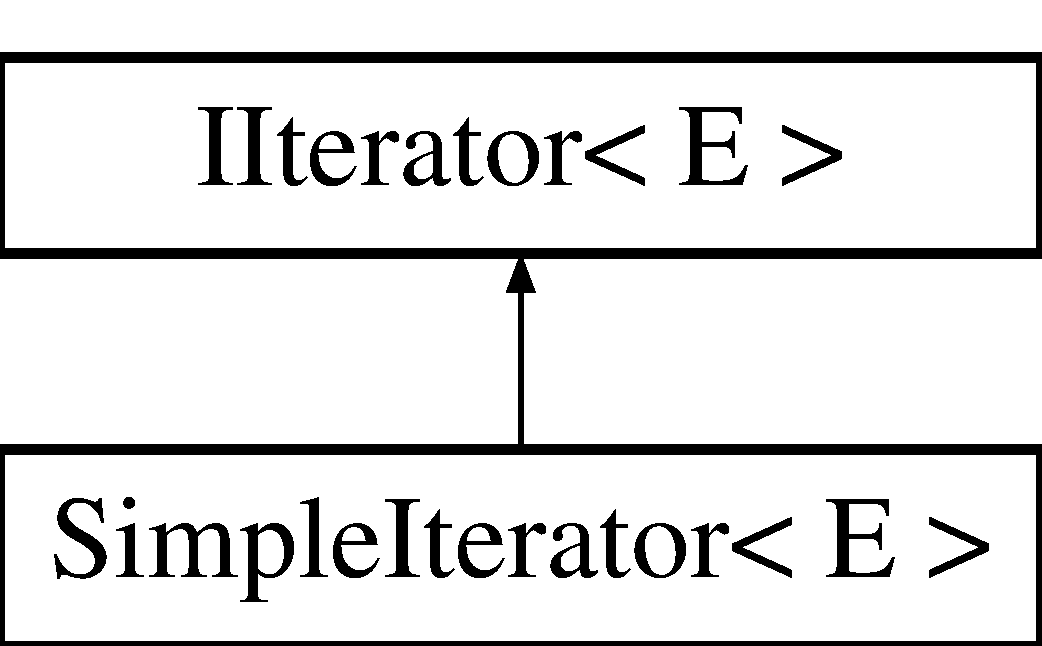
\includegraphics[height=2.000000cm]{class_simple_iterator}
\end{center}
\end{figure}
\subsection*{Public Member Functions}
\begin{DoxyCompactItemize}
\item 
\hyperlink{class_simple_iterator_a643cab8769a566826092a5db6ace3267}{Simple\-Iterator} (\hyperlink{class_node}{Node}$<$ E $>$ $\ast$, \hyperlink{class_node}{Node}$<$ E $>$ $\ast$)
\begin{DoxyCompactList}\small\item\em Metodo constructor. \end{DoxyCompactList}\item 
E \hyperlink{class_simple_iterator_ab01032dba9ff4f1a1c47af3082b717d5}{get\-Next} ()
\begin{DoxyCompactList}\small\item\em Obtiene el dato actual y actualiza al nodo siguiente. \end{DoxyCompactList}\item 
E \hyperlink{class_simple_iterator_ac9460c98985a20f781f351c85b8a3ba2}{get\-Current} () const 
\begin{DoxyCompactList}\small\item\em Obtiene el dato actual. \end{DoxyCompactList}\item 
bool \hyperlink{class_simple_iterator_ab946b3d707e32d4d53f15af201ea2113}{has\-Next} () const 
\begin{DoxyCompactList}\small\item\em Verifica si tiene siguiente. \end{DoxyCompactList}\item 
virtual \hyperlink{class_simple_iterator_a02203109d263581340152408ebb120a2}{$\sim$\-Simple\-Iterator} ()
\begin{DoxyCompactList}\small\item\em Liberador de memoria. \end{DoxyCompactList}\end{DoxyCompactItemize}
\subsection*{Protected Attributes}
\begin{DoxyCompactItemize}
\item 
\hyperlink{class_node}{Node}$<$ E $>$ $\ast$ \hyperlink{class_simple_iterator_a0403100ab86dba958115cea4147508a7}{head}
\item 
\hyperlink{class_node}{Node}$<$ E $>$ $\ast$ \hyperlink{class_simple_iterator_a9bfb7d6c12bc1e8031b5c0869026415a}{tail}
\item 
\hyperlink{class_node}{Node}$<$ E $>$ $\ast$ \hyperlink{class_simple_iterator_a7777fefe265a5067ec9319d8c1a3e278}{current}
\end{DoxyCompactItemize}
\subsection*{Friends}
\begin{DoxyCompactItemize}
\item 
{\footnotesize template$<$class T $>$ }\\class \hyperlink{class_simple_iterator_a8740adf5dfdafdc64940ab42ed663bd2}{List}
\item 
{\footnotesize template$<$class M $>$ }\\class \hyperlink{class_simple_iterator_ade98163865dd2cf1343ae0a4dbba6b29}{Circular\-List}
\end{DoxyCompactItemize}


\subsection{Detailed Description}
\subsubsection*{template$<$class E$>$class Simple\-Iterator$<$ E $>$}

Esta clase es un iterador de las listas simples, ademas la actualizacion de la lista N\-O actualiza el iterador, por lo que el iterador es momentaneo. Es similar a una fotografia de una lista que no ha sido alterada si la lista se altera usando un iterador puede que el iterador falle. Por lo que es recomendable que la lista no se actualice mientras se usa un iterador. 

\subsection{Constructor \& Destructor Documentation}
\hypertarget{class_simple_iterator_a643cab8769a566826092a5db6ace3267}{\index{Simple\-Iterator@{Simple\-Iterator}!Simple\-Iterator@{Simple\-Iterator}}
\index{Simple\-Iterator@{Simple\-Iterator}!SimpleIterator@{Simple\-Iterator}}
\subsubsection[{Simple\-Iterator}]{\setlength{\rightskip}{0pt plus 5cm}template$<$class E $>$ {\bf Simple\-Iterator}$<$ E $>$\-::{\bf Simple\-Iterator} (
\begin{DoxyParamCaption}
\item[{{\bf Node}$<$ E $>$ $\ast$}]{phead, }
\item[{{\bf Node}$<$ E $>$ $\ast$}]{ptail}
\end{DoxyParamCaption}
)}}\label{class_simple_iterator_a643cab8769a566826092a5db6ace3267}


Metodo constructor. 


\begin{DoxyParams}{Parameters}
{\em head} & es la cabeza por donde se iniciara la iteracion \\
\hline
{\em tail} & es la cola el ultimo elemento de la iteracion \\
\hline
\end{DoxyParams}
\hypertarget{class_simple_iterator_a02203109d263581340152408ebb120a2}{\index{Simple\-Iterator@{Simple\-Iterator}!$\sim$\-Simple\-Iterator@{$\sim$\-Simple\-Iterator}}
\index{$\sim$\-Simple\-Iterator@{$\sim$\-Simple\-Iterator}!SimpleIterator@{Simple\-Iterator}}
\subsubsection[{$\sim$\-Simple\-Iterator}]{\setlength{\rightskip}{0pt plus 5cm}template$<$class E $>$ {\bf Simple\-Iterator}$<$ E $>$\-::$\sim${\bf Simple\-Iterator} (
\begin{DoxyParamCaption}
{}
\end{DoxyParamCaption}
)\hspace{0.3cm}{\ttfamily [virtual]}}}\label{class_simple_iterator_a02203109d263581340152408ebb120a2}


Liberador de memoria. 



\subsection{Member Function Documentation}
\hypertarget{class_simple_iterator_ac9460c98985a20f781f351c85b8a3ba2}{\index{Simple\-Iterator@{Simple\-Iterator}!get\-Current@{get\-Current}}
\index{get\-Current@{get\-Current}!SimpleIterator@{Simple\-Iterator}}
\subsubsection[{get\-Current}]{\setlength{\rightskip}{0pt plus 5cm}template$<$class E $>$ E {\bf Simple\-Iterator}$<$ E $>$\-::get\-Current (
\begin{DoxyParamCaption}
{}
\end{DoxyParamCaption}
) const\hspace{0.3cm}{\ttfamily [virtual]}}}\label{class_simple_iterator_ac9460c98985a20f781f351c85b8a3ba2}


Obtiene el dato actual. 

\begin{DoxyReturn}{Returns}
E el dato actual 
\end{DoxyReturn}

\begin{DoxyExceptions}{Exceptions}
{\em donthavenext} & si el dato actual es nulo \\
\hline
\end{DoxyExceptions}


Implements \hyperlink{class_i_iterator_a50f55ce1381378aad2c93f16c9b60822}{I\-Iterator$<$ E $>$}.

\hypertarget{class_simple_iterator_ab01032dba9ff4f1a1c47af3082b717d5}{\index{Simple\-Iterator@{Simple\-Iterator}!get\-Next@{get\-Next}}
\index{get\-Next@{get\-Next}!SimpleIterator@{Simple\-Iterator}}
\subsubsection[{get\-Next}]{\setlength{\rightskip}{0pt plus 5cm}template$<$class E $>$ E {\bf Simple\-Iterator}$<$ E $>$\-::get\-Next (
\begin{DoxyParamCaption}
{}
\end{DoxyParamCaption}
)\hspace{0.3cm}{\ttfamily [virtual]}}}\label{class_simple_iterator_ab01032dba9ff4f1a1c47af3082b717d5}


Obtiene el dato actual y actualiza al nodo siguiente. 

\begin{DoxyReturn}{Returns}
E el dato actual 
\end{DoxyReturn}

\begin{DoxyExceptions}{Exceptions}
{\em donthavenext} & si el dato actual es nulo \\
\hline
\end{DoxyExceptions}


Implements \hyperlink{class_i_iterator_ab1b13434e4fac20c74262dee51d1e870}{I\-Iterator$<$ E $>$}.

\hypertarget{class_simple_iterator_ab946b3d707e32d4d53f15af201ea2113}{\index{Simple\-Iterator@{Simple\-Iterator}!has\-Next@{has\-Next}}
\index{has\-Next@{has\-Next}!SimpleIterator@{Simple\-Iterator}}
\subsubsection[{has\-Next}]{\setlength{\rightskip}{0pt plus 5cm}template$<$class E $>$ bool {\bf Simple\-Iterator}$<$ E $>$\-::has\-Next (
\begin{DoxyParamCaption}
{}
\end{DoxyParamCaption}
) const\hspace{0.3cm}{\ttfamily [virtual]}}}\label{class_simple_iterator_ab946b3d707e32d4d53f15af201ea2113}


Verifica si tiene siguiente. 

\begin{DoxyReturn}{Returns}
true si tiene siguiente, false si no lo tiene 
\end{DoxyReturn}

\begin{DoxyExceptions}{Exceptions}
{\em donthavenext} & si el dato actual es nulo \\
\hline
\end{DoxyExceptions}


Implements \hyperlink{class_i_iterator_a8a73f0fb41a66fe98e5e636378759196}{I\-Iterator$<$ E $>$}.



\subsection{Friends And Related Function Documentation}
\hypertarget{class_simple_iterator_ade98163865dd2cf1343ae0a4dbba6b29}{\index{Simple\-Iterator@{Simple\-Iterator}!Circular\-List@{Circular\-List}}
\index{Circular\-List@{Circular\-List}!SimpleIterator@{Simple\-Iterator}}
\subsubsection[{Circular\-List}]{\setlength{\rightskip}{0pt plus 5cm}template$<$class E$>$ template$<$class M $>$ friend class {\bf Circular\-List}\hspace{0.3cm}{\ttfamily [friend]}}}\label{class_simple_iterator_ade98163865dd2cf1343ae0a4dbba6b29}
\hypertarget{class_simple_iterator_a8740adf5dfdafdc64940ab42ed663bd2}{\index{Simple\-Iterator@{Simple\-Iterator}!List@{List}}
\index{List@{List}!SimpleIterator@{Simple\-Iterator}}
\subsubsection[{List}]{\setlength{\rightskip}{0pt plus 5cm}template$<$class E$>$ template$<$class T $>$ friend class {\bf List}\hspace{0.3cm}{\ttfamily [friend]}}}\label{class_simple_iterator_a8740adf5dfdafdc64940ab42ed663bd2}


\subsection{Member Data Documentation}
\hypertarget{class_simple_iterator_a7777fefe265a5067ec9319d8c1a3e278}{\index{Simple\-Iterator@{Simple\-Iterator}!current@{current}}
\index{current@{current}!SimpleIterator@{Simple\-Iterator}}
\subsubsection[{current}]{\setlength{\rightskip}{0pt plus 5cm}template$<$class E$>$ {\bf Node}$<$E$>$ $\ast$ {\bf Simple\-Iterator}$<$ E $>$\-::current\hspace{0.3cm}{\ttfamily [protected]}}}\label{class_simple_iterator_a7777fefe265a5067ec9319d8c1a3e278}
T\-O\-D\-O \hypertarget{class_simple_iterator_a0403100ab86dba958115cea4147508a7}{\index{Simple\-Iterator@{Simple\-Iterator}!head@{head}}
\index{head@{head}!SimpleIterator@{Simple\-Iterator}}
\subsubsection[{head}]{\setlength{\rightskip}{0pt plus 5cm}template$<$class E$>$ {\bf Node}$<$E$>$$\ast$ {\bf Simple\-Iterator}$<$ E $>$\-::head\hspace{0.3cm}{\ttfamily [protected]}}}\label{class_simple_iterator_a0403100ab86dba958115cea4147508a7}
\hypertarget{class_simple_iterator_a9bfb7d6c12bc1e8031b5c0869026415a}{\index{Simple\-Iterator@{Simple\-Iterator}!tail@{tail}}
\index{tail@{tail}!SimpleIterator@{Simple\-Iterator}}
\subsubsection[{tail}]{\setlength{\rightskip}{0pt plus 5cm}template$<$class E$>$ {\bf Node}$<$E$>$ $\ast$ {\bf Simple\-Iterator}$<$ E $>$\-::tail\hspace{0.3cm}{\ttfamily [protected]}}}\label{class_simple_iterator_a9bfb7d6c12bc1e8031b5c0869026415a}


The documentation for this class was generated from the following file\-:\begin{DoxyCompactItemize}
\item 
list/\hyperlink{_simple_iterator_8h}{Simple\-Iterator.\-h}\end{DoxyCompactItemize}

\hypertarget{class_simple_list_adapter}{\section{Simple\-List\-Adapter$<$ E $>$ Class Template Reference}
\label{class_simple_list_adapter}\index{Simple\-List\-Adapter$<$ E $>$@{Simple\-List\-Adapter$<$ E $>$}}
}


{\ttfamily \#include $<$simplelistadapter.\-h$>$}

Inheritance diagram for Simple\-List\-Adapter$<$ E $>$\-:\begin{figure}[H]
\begin{center}
\leavevmode
\includegraphics[height=3.000000cm]{class_simple_list_adapter}
\end{center}
\end{figure}
\subsection*{Public Member Functions}
\begin{DoxyCompactItemize}
\item 
bool \hyperlink{class_simple_list_adapter_a659e4b834a3d5dc46e25665c7809a3d8}{add} (E p\-Data)
\item 
bool \hyperlink{class_simple_list_adapter_a459ccf5fdce99a9b6dade7d187fb2e8d}{remove} (int p\-Index)
\item 
E \hyperlink{class_simple_list_adapter_a0dd35a961e4c7311cb82c11782340667}{get} (int p\-Index)
\item 
E \& \hyperlink{class_simple_list_adapter_aa548a9578aa7288205982062834e00e9}{get\-Reference} (int p\-Index)
\item 
\hyperlink{class_i_iterator}{I\-Iterator}$<$ E $>$ $\ast$ \hyperlink{class_simple_list_adapter_a32e8dd965e56d402fe5b450ecc7c7d3c}{get\-Iterator} ()
\item 
void \hyperlink{class_simple_list_adapter_ae2e5fe821e64b93c93eeda590d31f5f2}{print} ()
\item 
virtual \hyperlink{class_simple_list_adapter_a8bc601004a917aa5823bb5117391ddd6}{$\sim$\-Simple\-List\-Adapter} ()
\end{DoxyCompactItemize}
\subsection*{Protected Member Functions}
\begin{DoxyCompactItemize}
\item 
virtual bool \hyperlink{class_simple_list_adapter_abfd8b7cecf59921fb985f2121e246c99}{addi} (E p\-Data)=0
\item 
virtual bool \hyperlink{class_simple_list_adapter_a89d3c954a3782181f871b30c7a726379}{addf} (E p\-Data)=0
\item 
virtual bool \hyperlink{class_simple_list_adapter_a269a73b10beb87dddb3330af47334522}{add\-First\-Data} (E p\-Data)=0
\item 
virtual bool \hyperlink{class_simple_list_adapter_a9bebc8a42330e453f6e608e54de36adf}{removei} ()=0
\item 
virtual bool \hyperlink{class_simple_list_adapter_a9008dff51a5a156c0929b972e59e8f1d}{removef} ()=0
\end{DoxyCompactItemize}
\subsection*{Protected Attributes}
\begin{DoxyCompactItemize}
\item 
\hyperlink{class_node}{Node}$<$ E $>$ $\ast$ \hyperlink{class_simple_list_adapter_af8279a43660863dbf56cc31d27c331df}{\-\_\-head}
\item 
\hyperlink{class_node}{Node}$<$ E $>$ $\ast$ \hyperlink{class_simple_list_adapter_aee311f35611a7a15c68ee78ea5b7394c}{\-\_\-tail}
\end{DoxyCompactItemize}


\subsection{Constructor \& Destructor Documentation}
\hypertarget{class_simple_list_adapter_a8bc601004a917aa5823bb5117391ddd6}{\index{Simple\-List\-Adapter@{Simple\-List\-Adapter}!$\sim$\-Simple\-List\-Adapter@{$\sim$\-Simple\-List\-Adapter}}
\index{$\sim$\-Simple\-List\-Adapter@{$\sim$\-Simple\-List\-Adapter}!SimpleListAdapter@{Simple\-List\-Adapter}}
\subsubsection[{$\sim$\-Simple\-List\-Adapter}]{\setlength{\rightskip}{0pt plus 5cm}template$<$class E $>$ {\bf Simple\-List\-Adapter}$<$ E $>$\-::$\sim${\bf Simple\-List\-Adapter} (
\begin{DoxyParamCaption}
{}
\end{DoxyParamCaption}
)\hspace{0.3cm}{\ttfamily [virtual]}}}\label{class_simple_list_adapter_a8bc601004a917aa5823bb5117391ddd6}


\subsection{Member Function Documentation}
\hypertarget{class_simple_list_adapter_a659e4b834a3d5dc46e25665c7809a3d8}{\index{Simple\-List\-Adapter@{Simple\-List\-Adapter}!add@{add}}
\index{add@{add}!SimpleListAdapter@{Simple\-List\-Adapter}}
\subsubsection[{add}]{\setlength{\rightskip}{0pt plus 5cm}template$<$class E$>$ bool {\bf Simple\-List\-Adapter}$<$ E $>$\-::add (
\begin{DoxyParamCaption}
\item[{E}]{p\-Data}
\end{DoxyParamCaption}
)\hspace{0.3cm}{\ttfamily [virtual]}}}\label{class_simple_list_adapter_a659e4b834a3d5dc46e25665c7809a3d8}


Implements \hyperlink{class_i_ordinate_list_af158c9cda23201b2a17e857ffcdf4cdd}{I\-Ordinate\-List$<$ E $>$}.

\hypertarget{class_simple_list_adapter_a89d3c954a3782181f871b30c7a726379}{\index{Simple\-List\-Adapter@{Simple\-List\-Adapter}!addf@{addf}}
\index{addf@{addf}!SimpleListAdapter@{Simple\-List\-Adapter}}
\subsubsection[{addf}]{\setlength{\rightskip}{0pt plus 5cm}template$<$class E$>$ virtual bool {\bf Simple\-List\-Adapter}$<$ E $>$\-::addf (
\begin{DoxyParamCaption}
\item[{E}]{p\-Data}
\end{DoxyParamCaption}
)\hspace{0.3cm}{\ttfamily [protected]}, {\ttfamily [pure virtual]}}}\label{class_simple_list_adapter_a89d3c954a3782181f871b30c7a726379}


Implemented in \hyperlink{class_circular_list_ad2832eb48d7d69fa5d759c0c16c4bc5e}{Circular\-List$<$ E $>$}, \hyperlink{class_list_a3c920f9c86d2853121c5cd2fb46f8436}{List$<$ E $>$}, \hyperlink{class_circular_list_ad2832eb48d7d69fa5d759c0c16c4bc5e}{Circular\-List$<$ Shot\-Fabric $\ast$ $>$}, \hyperlink{class_list_a3c920f9c86d2853121c5cd2fb46f8436}{List$<$ Player $\ast$ $>$}, \hyperlink{class_list_a3c920f9c86d2853121c5cd2fb46f8436}{List$<$ Shot $\ast$ $>$}, \hyperlink{class_list_a3c920f9c86d2853121c5cd2fb46f8436}{List$<$ Q\-Rect $>$}, and \hyperlink{class_list_a3c920f9c86d2853121c5cd2fb46f8436}{List$<$ Enemy\-Rocket $\ast$ $>$}.

\hypertarget{class_simple_list_adapter_a269a73b10beb87dddb3330af47334522}{\index{Simple\-List\-Adapter@{Simple\-List\-Adapter}!add\-First\-Data@{add\-First\-Data}}
\index{add\-First\-Data@{add\-First\-Data}!SimpleListAdapter@{Simple\-List\-Adapter}}
\subsubsection[{add\-First\-Data}]{\setlength{\rightskip}{0pt plus 5cm}template$<$class E$>$ virtual bool {\bf Simple\-List\-Adapter}$<$ E $>$\-::add\-First\-Data (
\begin{DoxyParamCaption}
\item[{E}]{p\-Data}
\end{DoxyParamCaption}
)\hspace{0.3cm}{\ttfamily [protected]}, {\ttfamily [pure virtual]}}}\label{class_simple_list_adapter_a269a73b10beb87dddb3330af47334522}


Implemented in \hyperlink{class_circular_list_a0a3f318454d748eff1e3b8729aea94bd}{Circular\-List$<$ E $>$}, \hyperlink{class_list_ac38635d10f3faaf49af53c0b66347d0f}{List$<$ E $>$}, \hyperlink{class_circular_list_a0a3f318454d748eff1e3b8729aea94bd}{Circular\-List$<$ Shot\-Fabric $\ast$ $>$}, \hyperlink{class_list_ac38635d10f3faaf49af53c0b66347d0f}{List$<$ Player $\ast$ $>$}, \hyperlink{class_list_ac38635d10f3faaf49af53c0b66347d0f}{List$<$ Shot $\ast$ $>$}, \hyperlink{class_list_ac38635d10f3faaf49af53c0b66347d0f}{List$<$ Q\-Rect $>$}, and \hyperlink{class_list_ac38635d10f3faaf49af53c0b66347d0f}{List$<$ Enemy\-Rocket $\ast$ $>$}.

\hypertarget{class_simple_list_adapter_abfd8b7cecf59921fb985f2121e246c99}{\index{Simple\-List\-Adapter@{Simple\-List\-Adapter}!addi@{addi}}
\index{addi@{addi}!SimpleListAdapter@{Simple\-List\-Adapter}}
\subsubsection[{addi}]{\setlength{\rightskip}{0pt plus 5cm}template$<$class E$>$ virtual bool {\bf Simple\-List\-Adapter}$<$ E $>$\-::addi (
\begin{DoxyParamCaption}
\item[{E}]{p\-Data}
\end{DoxyParamCaption}
)\hspace{0.3cm}{\ttfamily [protected]}, {\ttfamily [pure virtual]}}}\label{class_simple_list_adapter_abfd8b7cecf59921fb985f2121e246c99}


Implemented in \hyperlink{class_circular_list_a275c75e142e791de9a1a00691af56a73}{Circular\-List$<$ E $>$}, \hyperlink{class_circular_list_a275c75e142e791de9a1a00691af56a73}{Circular\-List$<$ Shot\-Fabric $\ast$ $>$}, \hyperlink{class_list_a4f0fb366c1153a4fd01826e9e6de5afc}{List$<$ E $>$}, \hyperlink{class_list_a4f0fb366c1153a4fd01826e9e6de5afc}{List$<$ Player $\ast$ $>$}, \hyperlink{class_list_a4f0fb366c1153a4fd01826e9e6de5afc}{List$<$ Shot $\ast$ $>$}, \hyperlink{class_list_a4f0fb366c1153a4fd01826e9e6de5afc}{List$<$ Q\-Rect $>$}, \hyperlink{class_list_a4f0fb366c1153a4fd01826e9e6de5afc}{List$<$ Enemy\-Rocket $\ast$ $>$}, \hyperlink{class_circular_list_a6f405f4be7946286a958e0b83937b3e2}{Circular\-List$<$ E $>$}, \hyperlink{class_list_a92ad933f8d3a033b84a517fb6cc4111a}{List$<$ E $>$}, \hyperlink{class_circular_list_a6f405f4be7946286a958e0b83937b3e2}{Circular\-List$<$ Shot\-Fabric $\ast$ $>$}, \hyperlink{class_list_a92ad933f8d3a033b84a517fb6cc4111a}{List$<$ Player $\ast$ $>$}, \hyperlink{class_list_a92ad933f8d3a033b84a517fb6cc4111a}{List$<$ Shot $\ast$ $>$}, \hyperlink{class_list_a92ad933f8d3a033b84a517fb6cc4111a}{List$<$ Q\-Rect $>$}, and \hyperlink{class_list_a92ad933f8d3a033b84a517fb6cc4111a}{List$<$ Enemy\-Rocket $\ast$ $>$}.

\hypertarget{class_simple_list_adapter_a0dd35a961e4c7311cb82c11782340667}{\index{Simple\-List\-Adapter@{Simple\-List\-Adapter}!get@{get}}
\index{get@{get}!SimpleListAdapter@{Simple\-List\-Adapter}}
\subsubsection[{get}]{\setlength{\rightskip}{0pt plus 5cm}template$<$class E $>$ E {\bf Simple\-List\-Adapter}$<$ E $>$\-::get (
\begin{DoxyParamCaption}
\item[{int}]{p\-Index}
\end{DoxyParamCaption}
)\hspace{0.3cm}{\ttfamily [virtual]}}}\label{class_simple_list_adapter_a0dd35a961e4c7311cb82c11782340667}


Implements \hyperlink{class_i_ordinate_list_aef65b00ca705d1b106d51bff512b2021}{I\-Ordinate\-List$<$ E $>$}.

\hypertarget{class_simple_list_adapter_a32e8dd965e56d402fe5b450ecc7c7d3c}{\index{Simple\-List\-Adapter@{Simple\-List\-Adapter}!get\-Iterator@{get\-Iterator}}
\index{get\-Iterator@{get\-Iterator}!SimpleListAdapter@{Simple\-List\-Adapter}}
\subsubsection[{get\-Iterator}]{\setlength{\rightskip}{0pt plus 5cm}template$<$class E $>$ {\bf I\-Iterator}$<$ E $>$ $\ast$ {\bf Simple\-List\-Adapter}$<$ E $>$\-::get\-Iterator (
\begin{DoxyParamCaption}
{}
\end{DoxyParamCaption}
)\hspace{0.3cm}{\ttfamily [virtual]}}}\label{class_simple_list_adapter_a32e8dd965e56d402fe5b450ecc7c7d3c}


Implements \hyperlink{class_i_ordinate_list_aa555ab647394d5bf06bb4f38715bd167}{I\-Ordinate\-List$<$ E $>$}.

\hypertarget{class_simple_list_adapter_aa548a9578aa7288205982062834e00e9}{\index{Simple\-List\-Adapter@{Simple\-List\-Adapter}!get\-Reference@{get\-Reference}}
\index{get\-Reference@{get\-Reference}!SimpleListAdapter@{Simple\-List\-Adapter}}
\subsubsection[{get\-Reference}]{\setlength{\rightskip}{0pt plus 5cm}template$<$class E $>$ E \& {\bf Simple\-List\-Adapter}$<$ E $>$\-::get\-Reference (
\begin{DoxyParamCaption}
\item[{int}]{p\-Index}
\end{DoxyParamCaption}
)\hspace{0.3cm}{\ttfamily [virtual]}}}\label{class_simple_list_adapter_aa548a9578aa7288205982062834e00e9}


Implements \hyperlink{class_i_ordinate_list_a126adb3087d227a7bd47288002c6d48e}{I\-Ordinate\-List$<$ E $>$}.

\hypertarget{class_simple_list_adapter_ae2e5fe821e64b93c93eeda590d31f5f2}{\index{Simple\-List\-Adapter@{Simple\-List\-Adapter}!print@{print}}
\index{print@{print}!SimpleListAdapter@{Simple\-List\-Adapter}}
\subsubsection[{print}]{\setlength{\rightskip}{0pt plus 5cm}template$<$class E $>$ void {\bf Simple\-List\-Adapter}$<$ E $>$\-::print (
\begin{DoxyParamCaption}
{}
\end{DoxyParamCaption}
)}}\label{class_simple_list_adapter_ae2e5fe821e64b93c93eeda590d31f5f2}
\hypertarget{class_simple_list_adapter_a459ccf5fdce99a9b6dade7d187fb2e8d}{\index{Simple\-List\-Adapter@{Simple\-List\-Adapter}!remove@{remove}}
\index{remove@{remove}!SimpleListAdapter@{Simple\-List\-Adapter}}
\subsubsection[{remove}]{\setlength{\rightskip}{0pt plus 5cm}template$<$class E $>$ bool {\bf Simple\-List\-Adapter}$<$ E $>$\-::remove (
\begin{DoxyParamCaption}
\item[{int}]{p\-Index}
\end{DoxyParamCaption}
)\hspace{0.3cm}{\ttfamily [virtual]}}}\label{class_simple_list_adapter_a459ccf5fdce99a9b6dade7d187fb2e8d}


Implements \hyperlink{class_i_ordinate_list_a1015be27579a09c4805505ea3e4c4752}{I\-Ordinate\-List$<$ E $>$}.

\hypertarget{class_simple_list_adapter_a9008dff51a5a156c0929b972e59e8f1d}{\index{Simple\-List\-Adapter@{Simple\-List\-Adapter}!removef@{removef}}
\index{removef@{removef}!SimpleListAdapter@{Simple\-List\-Adapter}}
\subsubsection[{removef}]{\setlength{\rightskip}{0pt plus 5cm}template$<$class E$>$ virtual bool {\bf Simple\-List\-Adapter}$<$ E $>$\-::removef (
\begin{DoxyParamCaption}
{}
\end{DoxyParamCaption}
)\hspace{0.3cm}{\ttfamily [protected]}, {\ttfamily [pure virtual]}}}\label{class_simple_list_adapter_a9008dff51a5a156c0929b972e59e8f1d}


Implemented in \hyperlink{class_circular_list_a1dde06b77306b31eb38fa4b43b6009ab}{Circular\-List$<$ E $>$}, \hyperlink{class_list_a45231b54bf8c98948becddd0923be138}{List$<$ E $>$}, \hyperlink{class_circular_list_a1dde06b77306b31eb38fa4b43b6009ab}{Circular\-List$<$ Shot\-Fabric $\ast$ $>$}, \hyperlink{class_list_a45231b54bf8c98948becddd0923be138}{List$<$ Player $\ast$ $>$}, \hyperlink{class_list_a45231b54bf8c98948becddd0923be138}{List$<$ Shot $\ast$ $>$}, \hyperlink{class_list_a45231b54bf8c98948becddd0923be138}{List$<$ Q\-Rect $>$}, and \hyperlink{class_list_a45231b54bf8c98948becddd0923be138}{List$<$ Enemy\-Rocket $\ast$ $>$}.

\hypertarget{class_simple_list_adapter_a9bebc8a42330e453f6e608e54de36adf}{\index{Simple\-List\-Adapter@{Simple\-List\-Adapter}!removei@{removei}}
\index{removei@{removei}!SimpleListAdapter@{Simple\-List\-Adapter}}
\subsubsection[{removei}]{\setlength{\rightskip}{0pt plus 5cm}template$<$class E$>$ virtual bool {\bf Simple\-List\-Adapter}$<$ E $>$\-::removei (
\begin{DoxyParamCaption}
{}
\end{DoxyParamCaption}
)\hspace{0.3cm}{\ttfamily [protected]}, {\ttfamily [pure virtual]}}}\label{class_simple_list_adapter_a9bebc8a42330e453f6e608e54de36adf}


Implemented in \hyperlink{class_circular_list_a706dd0ab6fb475bec90d9c40cefa92b1}{Circular\-List$<$ E $>$}, \hyperlink{class_list_a1d0a5649ddd83cb781174698f80b2e0f}{List$<$ E $>$}, \hyperlink{class_circular_list_a706dd0ab6fb475bec90d9c40cefa92b1}{Circular\-List$<$ Shot\-Fabric $\ast$ $>$}, \hyperlink{class_list_a1d0a5649ddd83cb781174698f80b2e0f}{List$<$ Player $\ast$ $>$}, \hyperlink{class_list_a1d0a5649ddd83cb781174698f80b2e0f}{List$<$ Shot $\ast$ $>$}, \hyperlink{class_list_a1d0a5649ddd83cb781174698f80b2e0f}{List$<$ Q\-Rect $>$}, and \hyperlink{class_list_a1d0a5649ddd83cb781174698f80b2e0f}{List$<$ Enemy\-Rocket $\ast$ $>$}.



\subsection{Member Data Documentation}
\hypertarget{class_simple_list_adapter_af8279a43660863dbf56cc31d27c331df}{\index{Simple\-List\-Adapter@{Simple\-List\-Adapter}!\-\_\-head@{\-\_\-head}}
\index{\-\_\-head@{\-\_\-head}!SimpleListAdapter@{Simple\-List\-Adapter}}
\subsubsection[{\-\_\-head}]{\setlength{\rightskip}{0pt plus 5cm}template$<$class E$>$ {\bf Node}$<$E$>$$\ast$ {\bf Simple\-List\-Adapter}$<$ E $>$\-::\-\_\-head\hspace{0.3cm}{\ttfamily [protected]}}}\label{class_simple_list_adapter_af8279a43660863dbf56cc31d27c331df}
\hypertarget{class_simple_list_adapter_aee311f35611a7a15c68ee78ea5b7394c}{\index{Simple\-List\-Adapter@{Simple\-List\-Adapter}!\-\_\-tail@{\-\_\-tail}}
\index{\-\_\-tail@{\-\_\-tail}!SimpleListAdapter@{Simple\-List\-Adapter}}
\subsubsection[{\-\_\-tail}]{\setlength{\rightskip}{0pt plus 5cm}template$<$class E$>$ {\bf Node}$<$E$>$ $\ast$ {\bf Simple\-List\-Adapter}$<$ E $>$\-::\-\_\-tail\hspace{0.3cm}{\ttfamily [protected]}}}\label{class_simple_list_adapter_aee311f35611a7a15c68ee78ea5b7394c}


The documentation for this class was generated from the following file\-:\begin{DoxyCompactItemize}
\item 
ordinate\-List/\hyperlink{simplelistadapter_8h}{simplelistadapter.\-h}\end{DoxyCompactItemize}

\hypertarget{class_socket}{\section{Socket Class Reference}
\label{class_socket}\index{Socket@{Socket}}
}


{\ttfamily \#include $<$socket.\-h$>$}

Inheritance diagram for Socket\-:\begin{figure}[H]
\begin{center}
\leavevmode
\includegraphics[height=2.000000cm]{class_socket}
\end{center}
\end{figure}
\subsection*{Public Member Functions}
\begin{DoxyCompactItemize}
\item 
\hyperlink{class_socket_a7c3256c4fc6e2c603df73201049fae5a}{Socket} ()
\item 
bool \hyperlink{class_socket_a6afde2dca985dacdfa770141192e2daf}{create} ()
\begin{DoxyCompactList}\small\item\em crea el socket de manera que inicializa sus valores \end{DoxyCompactList}\item 
bool \hyperlink{class_socket_a77afe3664d8996221a5d9a08a0330778}{link\-To\-Port} (const int p\-Port)
\begin{DoxyCompactList}\small\item\em link\-To\-Port, Enlazarse a un puerto \end{DoxyCompactList}\item 
bool \hyperlink{class_socket_ac841ace3ba3f3b0daa9b59a498d3769c}{listen} ()
\begin{DoxyCompactList}\small\item\em listen, escucha algo mediante el socket \end{DoxyCompactList}\item 
bool \hyperlink{class_socket_a0d133d518a86bfae2db9095c587aa4e3}{accept} (\hyperlink{class_socket}{Socket} \&p\-Other\-Socket)
\item 
bool \hyperlink{class_socket_a5ccaf81da2b6f25dded056e6dbf7f410}{is\-Valid} ()
\begin{DoxyCompactList}\small\item\em Retorna si el socket es valido. \end{DoxyCompactList}\item 
bool \hyperlink{class_socket_a5d4ef6f01022b2653aad96868bd87999}{send\-Message} (std\-::string message) const 
\begin{DoxyCompactList}\small\item\em Envia un mensaje. \end{DoxyCompactList}\item 
int \hyperlink{class_socket_a80aef7d019680c494f45cbd5b7fa37f2}{receive\-Message} (std\-::string \&message) const 
\begin{DoxyCompactList}\small\item\em receive\-Message \end{DoxyCompactList}\item 
bool \hyperlink{class_socket_afe535648cf44461c6ded1b2d72056d47}{connect} (const std\-::string host, const int port)
\begin{DoxyCompactList}\small\item\em connect \end{DoxyCompactList}\item 
void \hyperlink{class_socket_ad97992fa51319cdf4d5d75c8bb49d100}{set\-Non\-Blocking} (const bool \hyperlink{jquery_8js_a2fa551895933fae935a0a6b87282241d}{b})
\begin{DoxyCompactList}\small\item\em set\-Non\-Blocking \end{DoxyCompactList}\item 
virtual \hyperlink{class_socket_aeac4eb6379a543d38ed88977d3b6630a}{$\sim$\-Socket} ()
\end{DoxyCompactItemize}
\subsection*{Static Public Attributes}
\begin{DoxyCompactItemize}
\item 
static const int \hyperlink{class_socket_a95e54f0602448bae84d85145a8720997}{M\-A\-X\-I\-M\-U\-N\-\_\-\-L\-E\-N\-G\-T\-H\-\_\-\-T\-O\-\_\-\-R\-E\-C\-E\-I\-V\-E} = 400
\item 
static const int \hyperlink{class_socket_a7e2ace3442918efea281250bf3833d06}{M\-A\-X\-I\-M\-U\-N\-\_\-\-C\-O\-N\-N\-E\-C\-T\-I\-O\-N} = 5
\item 
static const int \hyperlink{class_socket_a41f1845f6cf98d227b32e15f0c9467db}{M\-A\-X\-I\-M\-U\-N\-\_\-\-H\-O\-S\-T\-\_\-\-N\-A\-M\-E} = 200
\end{DoxyCompactItemize}


\subsection{Constructor \& Destructor Documentation}
\hypertarget{class_socket_a7c3256c4fc6e2c603df73201049fae5a}{\index{Socket@{Socket}!Socket@{Socket}}
\index{Socket@{Socket}!Socket@{Socket}}
\subsubsection[{Socket}]{\setlength{\rightskip}{0pt plus 5cm}Socket\-::\-Socket (
\begin{DoxyParamCaption}
{}
\end{DoxyParamCaption}
)}}\label{class_socket_a7c3256c4fc6e2c603df73201049fae5a}
\hypertarget{class_socket_aeac4eb6379a543d38ed88977d3b6630a}{\index{Socket@{Socket}!$\sim$\-Socket@{$\sim$\-Socket}}
\index{$\sim$\-Socket@{$\sim$\-Socket}!Socket@{Socket}}
\subsubsection[{$\sim$\-Socket}]{\setlength{\rightskip}{0pt plus 5cm}Socket\-::$\sim$\-Socket (
\begin{DoxyParamCaption}
{}
\end{DoxyParamCaption}
)\hspace{0.3cm}{\ttfamily [virtual]}}}\label{class_socket_aeac4eb6379a543d38ed88977d3b6630a}


\subsection{Member Function Documentation}
\hypertarget{class_socket_a0d133d518a86bfae2db9095c587aa4e3}{\index{Socket@{Socket}!accept@{accept}}
\index{accept@{accept}!Socket@{Socket}}
\subsubsection[{accept}]{\setlength{\rightskip}{0pt plus 5cm}bool Socket\-::accept (
\begin{DoxyParamCaption}
\item[{{\bf Socket} \&}]{p\-Other\-Socket}
\end{DoxyParamCaption}
)}}\label{class_socket_a0d133d518a86bfae2db9095c587aa4e3}
\hypertarget{class_socket_afe535648cf44461c6ded1b2d72056d47}{\index{Socket@{Socket}!connect@{connect}}
\index{connect@{connect}!Socket@{Socket}}
\subsubsection[{connect}]{\setlength{\rightskip}{0pt plus 5cm}bool Socket\-::connect (
\begin{DoxyParamCaption}
\item[{const std\-::string}]{host, }
\item[{const int}]{port}
\end{DoxyParamCaption}
)}}\label{class_socket_afe535648cf44461c6ded1b2d72056d47}


connect 


\begin{DoxyParams}{Parameters}
{\em host} & \\
\hline
{\em port} & \\
\hline
\end{DoxyParams}
\begin{DoxyReturn}{Returns}

\end{DoxyReturn}
\hypertarget{class_socket_a6afde2dca985dacdfa770141192e2daf}{\index{Socket@{Socket}!create@{create}}
\index{create@{create}!Socket@{Socket}}
\subsubsection[{create}]{\setlength{\rightskip}{0pt plus 5cm}bool Socket\-::create (
\begin{DoxyParamCaption}
{}
\end{DoxyParamCaption}
)}}\label{class_socket_a6afde2dca985dacdfa770141192e2daf}


crea el socket de manera que inicializa sus valores 

\begin{DoxyReturn}{Returns}
retorna si el socket fue creado exitosamente 
\end{DoxyReturn}
\hypertarget{class_socket_a5ccaf81da2b6f25dded056e6dbf7f410}{\index{Socket@{Socket}!is\-Valid@{is\-Valid}}
\index{is\-Valid@{is\-Valid}!Socket@{Socket}}
\subsubsection[{is\-Valid}]{\setlength{\rightskip}{0pt plus 5cm}bool Socket\-::is\-Valid (
\begin{DoxyParamCaption}
{}
\end{DoxyParamCaption}
)}}\label{class_socket_a5ccaf81da2b6f25dded056e6dbf7f410}


Retorna si el socket es valido. 

\begin{DoxyReturn}{Returns}

\end{DoxyReturn}
\hypertarget{class_socket_a77afe3664d8996221a5d9a08a0330778}{\index{Socket@{Socket}!link\-To\-Port@{link\-To\-Port}}
\index{link\-To\-Port@{link\-To\-Port}!Socket@{Socket}}
\subsubsection[{link\-To\-Port}]{\setlength{\rightskip}{0pt plus 5cm}bool Socket\-::link\-To\-Port (
\begin{DoxyParamCaption}
\item[{const int}]{p\-Port}
\end{DoxyParamCaption}
)}}\label{class_socket_a77afe3664d8996221a5d9a08a0330778}


link\-To\-Port, Enlazarse a un puerto 


\begin{DoxyParams}{Parameters}
{\em p\-Port} & puerto de coneccion \\
\hline
\end{DoxyParams}
\begin{DoxyReturn}{Returns}
true, si el enlace pudo realizarse con exito 
\end{DoxyReturn}
\hypertarget{class_socket_ac841ace3ba3f3b0daa9b59a498d3769c}{\index{Socket@{Socket}!listen@{listen}}
\index{listen@{listen}!Socket@{Socket}}
\subsubsection[{listen}]{\setlength{\rightskip}{0pt plus 5cm}bool Socket\-::listen (
\begin{DoxyParamCaption}
{}
\end{DoxyParamCaption}
)}}\label{class_socket_ac841ace3ba3f3b0daa9b59a498d3769c}


listen, escucha algo mediante el socket 

\begin{DoxyReturn}{Returns}
true, si escucha algo por medio del socket de conexion 
\end{DoxyReturn}
\hypertarget{class_socket_a80aef7d019680c494f45cbd5b7fa37f2}{\index{Socket@{Socket}!receive\-Message@{receive\-Message}}
\index{receive\-Message@{receive\-Message}!Socket@{Socket}}
\subsubsection[{receive\-Message}]{\setlength{\rightskip}{0pt plus 5cm}int Socket\-::receive\-Message (
\begin{DoxyParamCaption}
\item[{std\-::string \&}]{message}
\end{DoxyParamCaption}
) const}}\label{class_socket_a80aef7d019680c494f45cbd5b7fa37f2}


receive\-Message 


\begin{DoxyParams}{Parameters}
{\em message} & \\
\hline
\end{DoxyParams}
\begin{DoxyReturn}{Returns}

\end{DoxyReturn}
\hypertarget{class_socket_a5d4ef6f01022b2653aad96868bd87999}{\index{Socket@{Socket}!send\-Message@{send\-Message}}
\index{send\-Message@{send\-Message}!Socket@{Socket}}
\subsubsection[{send\-Message}]{\setlength{\rightskip}{0pt plus 5cm}bool Socket\-::send\-Message (
\begin{DoxyParamCaption}
\item[{std\-::string}]{message}
\end{DoxyParamCaption}
) const}}\label{class_socket_a5d4ef6f01022b2653aad96868bd87999}


Envia un mensaje. 


\begin{DoxyParams}{Parameters}
{\em message} & es el mensaje que se desea enviar \\
\hline
\end{DoxyParams}
\begin{DoxyReturn}{Returns}
si el mensaje fue enviado 
\end{DoxyReturn}
\hypertarget{class_socket_ad97992fa51319cdf4d5d75c8bb49d100}{\index{Socket@{Socket}!set\-Non\-Blocking@{set\-Non\-Blocking}}
\index{set\-Non\-Blocking@{set\-Non\-Blocking}!Socket@{Socket}}
\subsubsection[{set\-Non\-Blocking}]{\setlength{\rightskip}{0pt plus 5cm}void Socket\-::set\-Non\-Blocking (
\begin{DoxyParamCaption}
\item[{const bool}]{b}
\end{DoxyParamCaption}
)}}\label{class_socket_ad97992fa51319cdf4d5d75c8bb49d100}


set\-Non\-Blocking 


\begin{DoxyParams}{Parameters}
{\em b} & \\
\hline
\end{DoxyParams}


\subsection{Member Data Documentation}
\hypertarget{class_socket_a7e2ace3442918efea281250bf3833d06}{\index{Socket@{Socket}!M\-A\-X\-I\-M\-U\-N\-\_\-\-C\-O\-N\-N\-E\-C\-T\-I\-O\-N@{M\-A\-X\-I\-M\-U\-N\-\_\-\-C\-O\-N\-N\-E\-C\-T\-I\-O\-N}}
\index{M\-A\-X\-I\-M\-U\-N\-\_\-\-C\-O\-N\-N\-E\-C\-T\-I\-O\-N@{M\-A\-X\-I\-M\-U\-N\-\_\-\-C\-O\-N\-N\-E\-C\-T\-I\-O\-N}!Socket@{Socket}}
\subsubsection[{M\-A\-X\-I\-M\-U\-N\-\_\-\-C\-O\-N\-N\-E\-C\-T\-I\-O\-N}]{\setlength{\rightskip}{0pt plus 5cm}const int Socket\-::\-M\-A\-X\-I\-M\-U\-N\-\_\-\-C\-O\-N\-N\-E\-C\-T\-I\-O\-N = 5\hspace{0.3cm}{\ttfamily [static]}}}\label{class_socket_a7e2ace3442918efea281250bf3833d06}
\hypertarget{class_socket_a41f1845f6cf98d227b32e15f0c9467db}{\index{Socket@{Socket}!M\-A\-X\-I\-M\-U\-N\-\_\-\-H\-O\-S\-T\-\_\-\-N\-A\-M\-E@{M\-A\-X\-I\-M\-U\-N\-\_\-\-H\-O\-S\-T\-\_\-\-N\-A\-M\-E}}
\index{M\-A\-X\-I\-M\-U\-N\-\_\-\-H\-O\-S\-T\-\_\-\-N\-A\-M\-E@{M\-A\-X\-I\-M\-U\-N\-\_\-\-H\-O\-S\-T\-\_\-\-N\-A\-M\-E}!Socket@{Socket}}
\subsubsection[{M\-A\-X\-I\-M\-U\-N\-\_\-\-H\-O\-S\-T\-\_\-\-N\-A\-M\-E}]{\setlength{\rightskip}{0pt plus 5cm}const int Socket\-::\-M\-A\-X\-I\-M\-U\-N\-\_\-\-H\-O\-S\-T\-\_\-\-N\-A\-M\-E = 200\hspace{0.3cm}{\ttfamily [static]}}}\label{class_socket_a41f1845f6cf98d227b32e15f0c9467db}
\hypertarget{class_socket_a95e54f0602448bae84d85145a8720997}{\index{Socket@{Socket}!M\-A\-X\-I\-M\-U\-N\-\_\-\-L\-E\-N\-G\-T\-H\-\_\-\-T\-O\-\_\-\-R\-E\-C\-E\-I\-V\-E@{M\-A\-X\-I\-M\-U\-N\-\_\-\-L\-E\-N\-G\-T\-H\-\_\-\-T\-O\-\_\-\-R\-E\-C\-E\-I\-V\-E}}
\index{M\-A\-X\-I\-M\-U\-N\-\_\-\-L\-E\-N\-G\-T\-H\-\_\-\-T\-O\-\_\-\-R\-E\-C\-E\-I\-V\-E@{M\-A\-X\-I\-M\-U\-N\-\_\-\-L\-E\-N\-G\-T\-H\-\_\-\-T\-O\-\_\-\-R\-E\-C\-E\-I\-V\-E}!Socket@{Socket}}
\subsubsection[{M\-A\-X\-I\-M\-U\-N\-\_\-\-L\-E\-N\-G\-T\-H\-\_\-\-T\-O\-\_\-\-R\-E\-C\-E\-I\-V\-E}]{\setlength{\rightskip}{0pt plus 5cm}const int Socket\-::\-M\-A\-X\-I\-M\-U\-N\-\_\-\-L\-E\-N\-G\-T\-H\-\_\-\-T\-O\-\_\-\-R\-E\-C\-E\-I\-V\-E = 400\hspace{0.3cm}{\ttfamily [static]}}}\label{class_socket_a95e54f0602448bae84d85145a8720997}


The documentation for this class was generated from the following files\-:\begin{DoxyCompactItemize}
\item 
logic/lanconection/\hyperlink{socket_8h}{socket.\-h}\item 
logic/lanconection/\hyperlink{socket_8cpp}{socket.\-cpp}\end{DoxyCompactItemize}

\hypertarget{class_socket_exception}{\section{Socket\-Exception Class Reference}
\label{class_socket_exception}\index{Socket\-Exception@{Socket\-Exception}}
}
\subsection*{Public Member Functions}
\begin{DoxyCompactItemize}
\item 
\hypertarget{class_socket_exception_a4af250ab41b48e6167696cafb5a97165}{{\bfseries Socket\-Exception} (std\-::string p\-Message\-Warning)}\label{class_socket_exception_a4af250ab41b48e6167696cafb5a97165}

\item 
\hypertarget{class_socket_exception_a95a03e3ba3d78d27d23f8d4100f59e00}{std\-::string {\bfseries Message\-Warning} () const }\label{class_socket_exception_a95a03e3ba3d78d27d23f8d4100f59e00}

\item 
\hypertarget{class_socket_exception_ad7920caebddc99b6bbb7dbede569fa18}{std\-::string {\bfseries description} ()}\label{class_socket_exception_ad7920caebddc99b6bbb7dbede569fa18}

\end{DoxyCompactItemize}


The documentation for this class was generated from the following files\-:\begin{DoxyCompactItemize}
\item 
logic/lanconection/socketexception.\-h\item 
logic/lanconection/socketexception.\-cpp\end{DoxyCompactItemize}

\hypertarget{class_stack}{\section{Stack$<$ E $>$ Class Template Reference}
\label{class_stack}\index{Stack$<$ E $>$@{Stack$<$ E $>$}}
}


{\ttfamily \#include $<$Stack.\-h$>$}

\subsection*{Public Member Functions}
\begin{DoxyCompactItemize}
\item 
\hyperlink{class_stack_a561be1726ac9649a9ee3f80a4ca8e4b5}{Stack} ()
\begin{DoxyCompactList}\small\item\em Metodo constructor. \end{DoxyCompactList}\item 
void \hyperlink{class_stack_af71e3e142fba5bb861b66b4882289b31}{push} (E)
\begin{DoxyCompactList}\small\item\em Agrega el dato a la cima de la pila. \end{DoxyCompactList}\item 
E \hyperlink{class_stack_a5ba7a4c8eec39757e28f95da49f06d52}{pop} ()
\begin{DoxyCompactList}\small\item\em Elimina de la pila y retorna el dato de la cima de la pila. En caso de que la pila este vacia se produce un error. \end{DoxyCompactList}\item 
E \hyperlink{class_stack_a19a17240bf7045cf6a3a9497e1091433}{peek} () const 
\begin{DoxyCompactList}\small\item\em Revisa el dato en la cima de la pila. En caso de que la pila este vacia se produce un error. \end{DoxyCompactList}\item 
bool \hyperlink{class_stack_a0ce2804f35c0c8cfb999535f35fa438b}{is\-Empty} ()
\begin{DoxyCompactList}\small\item\em Retorna verdadero si la pila esta vacia de lo contrario retorna falso. \end{DoxyCompactList}\item 
virtual \hyperlink{class_stack_ad08e4c32f07b8d967913f8b1a45f8620}{$\sim$\-Stack} ()
\begin{DoxyCompactList}\small\item\em Metodo destructor, borra todos los elementos de la pila. \end{DoxyCompactList}\end{DoxyCompactItemize}


\subsection{Constructor \& Destructor Documentation}
\hypertarget{class_stack_a561be1726ac9649a9ee3f80a4ca8e4b5}{\index{Stack@{Stack}!Stack@{Stack}}
\index{Stack@{Stack}!Stack@{Stack}}
\subsubsection[{Stack}]{\setlength{\rightskip}{0pt plus 5cm}template$<$class E $>$ {\bf Stack}$<$ E $>$\-::{\bf Stack} (
\begin{DoxyParamCaption}
{}
\end{DoxyParamCaption}
)}}\label{class_stack_a561be1726ac9649a9ee3f80a4ca8e4b5}


Metodo constructor. 

\hypertarget{class_stack_ad08e4c32f07b8d967913f8b1a45f8620}{\index{Stack@{Stack}!$\sim$\-Stack@{$\sim$\-Stack}}
\index{$\sim$\-Stack@{$\sim$\-Stack}!Stack@{Stack}}
\subsubsection[{$\sim$\-Stack}]{\setlength{\rightskip}{0pt plus 5cm}template$<$class E $>$ {\bf Stack}$<$ E $>$\-::$\sim${\bf Stack} (
\begin{DoxyParamCaption}
{}
\end{DoxyParamCaption}
)\hspace{0.3cm}{\ttfamily [virtual]}}}\label{class_stack_ad08e4c32f07b8d967913f8b1a45f8620}


Metodo destructor, borra todos los elementos de la pila. 



\subsection{Member Function Documentation}
\hypertarget{class_stack_a0ce2804f35c0c8cfb999535f35fa438b}{\index{Stack@{Stack}!is\-Empty@{is\-Empty}}
\index{is\-Empty@{is\-Empty}!Stack@{Stack}}
\subsubsection[{is\-Empty}]{\setlength{\rightskip}{0pt plus 5cm}template$<$class E $>$ bool {\bf Stack}$<$ E $>$\-::is\-Empty (
\begin{DoxyParamCaption}
{}
\end{DoxyParamCaption}
)}}\label{class_stack_a0ce2804f35c0c8cfb999535f35fa438b}


Retorna verdadero si la pila esta vacia de lo contrario retorna falso. 

\begin{DoxyReturn}{Returns}
bool el valor de verdad de la frase ¿esta vacia la pila? 
\end{DoxyReturn}
\hypertarget{class_stack_a19a17240bf7045cf6a3a9497e1091433}{\index{Stack@{Stack}!peek@{peek}}
\index{peek@{peek}!Stack@{Stack}}
\subsubsection[{peek}]{\setlength{\rightskip}{0pt plus 5cm}template$<$class E $>$ E {\bf Stack}$<$ E $>$\-::peek (
\begin{DoxyParamCaption}
{}
\end{DoxyParamCaption}
) const}}\label{class_stack_a19a17240bf7045cf6a3a9497e1091433}


Revisa el dato en la cima de la pila. En caso de que la pila este vacia se produce un error. 

\begin{DoxyReturn}{Returns}
E el dato de la cima 
\end{DoxyReturn}
\hypertarget{class_stack_a5ba7a4c8eec39757e28f95da49f06d52}{\index{Stack@{Stack}!pop@{pop}}
\index{pop@{pop}!Stack@{Stack}}
\subsubsection[{pop}]{\setlength{\rightskip}{0pt plus 5cm}template$<$class E $>$ E {\bf Stack}$<$ E $>$\-::pop (
\begin{DoxyParamCaption}
{}
\end{DoxyParamCaption}
)}}\label{class_stack_a5ba7a4c8eec39757e28f95da49f06d52}


Elimina de la pila y retorna el dato de la cima de la pila. En caso de que la pila este vacia se produce un error. 

\begin{DoxyReturn}{Returns}
E el dato en la cima. 
\end{DoxyReturn}
\hypertarget{class_stack_af71e3e142fba5bb861b66b4882289b31}{\index{Stack@{Stack}!push@{push}}
\index{push@{push}!Stack@{Stack}}
\subsubsection[{push}]{\setlength{\rightskip}{0pt plus 5cm}template$<$class E $>$ void {\bf Stack}$<$ E $>$\-::push (
\begin{DoxyParamCaption}
\item[{E}]{data}
\end{DoxyParamCaption}
)}}\label{class_stack_af71e3e142fba5bb861b66b4882289b31}


Agrega el dato a la cima de la pila. 


\begin{DoxyParams}{Parameters}
{\em E} & el dato a agregar. \\
\hline
\end{DoxyParams}


The documentation for this class was generated from the following file\-:\begin{DoxyCompactItemize}
\item 
control\-Structure/\hyperlink{_stack_8h}{Stack.\-h}\end{DoxyCompactItemize}

\hypertarget{struct_static_descriptor_initializer___change_phase__2eproto}{\section{Static\-Descriptor\-Initializer\-\_\-\-Change\-Phase\-\_\-2eproto Struct Reference}
\label{struct_static_descriptor_initializer___change_phase__2eproto}\index{Static\-Descriptor\-Initializer\-\_\-\-Change\-Phase\-\_\-2eproto@{Static\-Descriptor\-Initializer\-\_\-\-Change\-Phase\-\_\-2eproto}}
}
\subsection*{Public Member Functions}
\begin{DoxyCompactItemize}
\item 
\hyperlink{struct_static_descriptor_initializer___change_phase__2eproto_afb3f28d8db6af6139ae353783bdebd28}{Static\-Descriptor\-Initializer\-\_\-\-Change\-Phase\-\_\-2eproto} ()
\end{DoxyCompactItemize}


\subsection{Constructor \& Destructor Documentation}
\hypertarget{struct_static_descriptor_initializer___change_phase__2eproto_afb3f28d8db6af6139ae353783bdebd28}{\index{Static\-Descriptor\-Initializer\-\_\-\-Change\-Phase\-\_\-2eproto@{Static\-Descriptor\-Initializer\-\_\-\-Change\-Phase\-\_\-2eproto}!Static\-Descriptor\-Initializer\-\_\-\-Change\-Phase\-\_\-2eproto@{Static\-Descriptor\-Initializer\-\_\-\-Change\-Phase\-\_\-2eproto}}
\index{Static\-Descriptor\-Initializer\-\_\-\-Change\-Phase\-\_\-2eproto@{Static\-Descriptor\-Initializer\-\_\-\-Change\-Phase\-\_\-2eproto}!StaticDescriptorInitializer_ChangePhase_2eproto@{Static\-Descriptor\-Initializer\-\_\-\-Change\-Phase\-\_\-2eproto}}
\subsubsection[{Static\-Descriptor\-Initializer\-\_\-\-Change\-Phase\-\_\-2eproto}]{\setlength{\rightskip}{0pt plus 5cm}Static\-Descriptor\-Initializer\-\_\-\-Change\-Phase\-\_\-2eproto\-::\-Static\-Descriptor\-Initializer\-\_\-\-Change\-Phase\-\_\-2eproto (
\begin{DoxyParamCaption}
{}
\end{DoxyParamCaption}
)\hspace{0.3cm}{\ttfamily [inline]}}}\label{struct_static_descriptor_initializer___change_phase__2eproto_afb3f28d8db6af6139ae353783bdebd28}


The documentation for this struct was generated from the following file\-:\begin{DoxyCompactItemize}
\item 
protobufmessage/\hyperlink{_change_phase_8pb_8cc}{Change\-Phase.\-pb.\-cc}\end{DoxyCompactItemize}

\hypertarget{struct_static_descriptor_initializer___control_player__2eproto}{\section{Static\-Descriptor\-Initializer\-\_\-\-Control\-Player\-\_\-2eproto Struct Reference}
\label{struct_static_descriptor_initializer___control_player__2eproto}\index{Static\-Descriptor\-Initializer\-\_\-\-Control\-Player\-\_\-2eproto@{Static\-Descriptor\-Initializer\-\_\-\-Control\-Player\-\_\-2eproto}}
}


The documentation for this struct was generated from the following file\-:\begin{DoxyCompactItemize}
\item 
protobufmessage/Control\-Player.\-pb.\-cc\end{DoxyCompactItemize}

\hypertarget{struct_static_descriptor_initializer___create_player__2eproto}{\section{Static\-Descriptor\-Initializer\-\_\-\-Create\-Player\-\_\-2eproto Struct Reference}
\label{struct_static_descriptor_initializer___create_player__2eproto}\index{Static\-Descriptor\-Initializer\-\_\-\-Create\-Player\-\_\-2eproto@{Static\-Descriptor\-Initializer\-\_\-\-Create\-Player\-\_\-2eproto}}
}


The documentation for this struct was generated from the following file\-:\begin{DoxyCompactItemize}
\item 
protobufmessage/Create\-Player.\-pb.\-cc\end{DoxyCompactItemize}

\hypertarget{struct_static_descriptor_initializer___game_menu__2eproto}{\section{Static\-Descriptor\-Initializer\-\_\-\-Game\-Menu\-\_\-2eproto Struct Reference}
\label{struct_static_descriptor_initializer___game_menu__2eproto}\index{Static\-Descriptor\-Initializer\-\_\-\-Game\-Menu\-\_\-2eproto@{Static\-Descriptor\-Initializer\-\_\-\-Game\-Menu\-\_\-2eproto}}
}


The documentation for this struct was generated from the following file\-:\begin{DoxyCompactItemize}
\item 
protobufmessage/Game\-Menu.\-pb.\-cc\end{DoxyCompactItemize}

\hypertarget{struct_static_descriptor_initializer___game_object_notify__2eproto}{\section{Static\-Descriptor\-Initializer\-\_\-\-Game\-Object\-Notify\-\_\-2eproto Struct Reference}
\label{struct_static_descriptor_initializer___game_object_notify__2eproto}\index{Static\-Descriptor\-Initializer\-\_\-\-Game\-Object\-Notify\-\_\-2eproto@{Static\-Descriptor\-Initializer\-\_\-\-Game\-Object\-Notify\-\_\-2eproto}}
}
\subsection*{Public Member Functions}
\begin{DoxyCompactItemize}
\item 
\hyperlink{struct_static_descriptor_initializer___game_object_notify__2eproto_aa4ae008d1cdff6840bcf8bf6fa07ab95}{Static\-Descriptor\-Initializer\-\_\-\-Game\-Object\-Notify\-\_\-2eproto} ()
\end{DoxyCompactItemize}


\subsection{Constructor \& Destructor Documentation}
\hypertarget{struct_static_descriptor_initializer___game_object_notify__2eproto_aa4ae008d1cdff6840bcf8bf6fa07ab95}{\index{Static\-Descriptor\-Initializer\-\_\-\-Game\-Object\-Notify\-\_\-2eproto@{Static\-Descriptor\-Initializer\-\_\-\-Game\-Object\-Notify\-\_\-2eproto}!Static\-Descriptor\-Initializer\-\_\-\-Game\-Object\-Notify\-\_\-2eproto@{Static\-Descriptor\-Initializer\-\_\-\-Game\-Object\-Notify\-\_\-2eproto}}
\index{Static\-Descriptor\-Initializer\-\_\-\-Game\-Object\-Notify\-\_\-2eproto@{Static\-Descriptor\-Initializer\-\_\-\-Game\-Object\-Notify\-\_\-2eproto}!StaticDescriptorInitializer_GameObjectNotify_2eproto@{Static\-Descriptor\-Initializer\-\_\-\-Game\-Object\-Notify\-\_\-2eproto}}
\subsubsection[{Static\-Descriptor\-Initializer\-\_\-\-Game\-Object\-Notify\-\_\-2eproto}]{\setlength{\rightskip}{0pt plus 5cm}Static\-Descriptor\-Initializer\-\_\-\-Game\-Object\-Notify\-\_\-2eproto\-::\-Static\-Descriptor\-Initializer\-\_\-\-Game\-Object\-Notify\-\_\-2eproto (
\begin{DoxyParamCaption}
{}
\end{DoxyParamCaption}
)\hspace{0.3cm}{\ttfamily [inline]}}}\label{struct_static_descriptor_initializer___game_object_notify__2eproto_aa4ae008d1cdff6840bcf8bf6fa07ab95}


The documentation for this struct was generated from the following file\-:\begin{DoxyCompactItemize}
\item 
protobufmessage/\hyperlink{_game_object_notify_8pb_8cc}{Game\-Object\-Notify.\-pb.\-cc}\end{DoxyCompactItemize}

\hypertarget{struct_static_descriptor_initializer___pause__2eproto}{\section{Static\-Descriptor\-Initializer\-\_\-\-Pause\-\_\-2eproto Struct Reference}
\label{struct_static_descriptor_initializer___pause__2eproto}\index{Static\-Descriptor\-Initializer\-\_\-\-Pause\-\_\-2eproto@{Static\-Descriptor\-Initializer\-\_\-\-Pause\-\_\-2eproto}}
}


The documentation for this struct was generated from the following file\-:\begin{DoxyCompactItemize}
\item 
protobufmessage/Pause.\-pb.\-cc\end{DoxyCompactItemize}

\hypertarget{struct_static_descriptor_initializer___pause_other_players__2eproto}{\section{Static\-Descriptor\-Initializer\-\_\-\-Pause\-Other\-Players\-\_\-2eproto Struct Reference}
\label{struct_static_descriptor_initializer___pause_other_players__2eproto}\index{Static\-Descriptor\-Initializer\-\_\-\-Pause\-Other\-Players\-\_\-2eproto@{Static\-Descriptor\-Initializer\-\_\-\-Pause\-Other\-Players\-\_\-2eproto}}
}
\subsection*{Public Member Functions}
\begin{DoxyCompactItemize}
\item 
\hyperlink{struct_static_descriptor_initializer___pause_other_players__2eproto_af2314feee2ff9f6028fcc9415323d6ad}{Static\-Descriptor\-Initializer\-\_\-\-Pause\-Other\-Players\-\_\-2eproto} ()
\end{DoxyCompactItemize}


\subsection{Constructor \& Destructor Documentation}
\hypertarget{struct_static_descriptor_initializer___pause_other_players__2eproto_af2314feee2ff9f6028fcc9415323d6ad}{\index{Static\-Descriptor\-Initializer\-\_\-\-Pause\-Other\-Players\-\_\-2eproto@{Static\-Descriptor\-Initializer\-\_\-\-Pause\-Other\-Players\-\_\-2eproto}!Static\-Descriptor\-Initializer\-\_\-\-Pause\-Other\-Players\-\_\-2eproto@{Static\-Descriptor\-Initializer\-\_\-\-Pause\-Other\-Players\-\_\-2eproto}}
\index{Static\-Descriptor\-Initializer\-\_\-\-Pause\-Other\-Players\-\_\-2eproto@{Static\-Descriptor\-Initializer\-\_\-\-Pause\-Other\-Players\-\_\-2eproto}!StaticDescriptorInitializer_PauseOtherPlayers_2eproto@{Static\-Descriptor\-Initializer\-\_\-\-Pause\-Other\-Players\-\_\-2eproto}}
\subsubsection[{Static\-Descriptor\-Initializer\-\_\-\-Pause\-Other\-Players\-\_\-2eproto}]{\setlength{\rightskip}{0pt plus 5cm}Static\-Descriptor\-Initializer\-\_\-\-Pause\-Other\-Players\-\_\-2eproto\-::\-Static\-Descriptor\-Initializer\-\_\-\-Pause\-Other\-Players\-\_\-2eproto (
\begin{DoxyParamCaption}
{}
\end{DoxyParamCaption}
)\hspace{0.3cm}{\ttfamily [inline]}}}\label{struct_static_descriptor_initializer___pause_other_players__2eproto_af2314feee2ff9f6028fcc9415323d6ad}


The documentation for this struct was generated from the following file\-:\begin{DoxyCompactItemize}
\item 
protobufmessage/\hyperlink{_pause_other_players_8pb_8cc}{Pause\-Other\-Players.\-pb.\-cc}\end{DoxyCompactItemize}

\hypertarget{struct_static_descriptor_initializer___player_is_created__2eproto}{\section{Static\-Descriptor\-Initializer\-\_\-\-Player\-Is\-Created\-\_\-2eproto Struct Reference}
\label{struct_static_descriptor_initializer___player_is_created__2eproto}\index{Static\-Descriptor\-Initializer\-\_\-\-Player\-Is\-Created\-\_\-2eproto@{Static\-Descriptor\-Initializer\-\_\-\-Player\-Is\-Created\-\_\-2eproto}}
}


The documentation for this struct was generated from the following file\-:\begin{DoxyCompactItemize}
\item 
protobufmessage/Player\-Is\-Created.\-pb.\-cc\end{DoxyCompactItemize}

\hypertarget{struct_static_descriptor_initializer___player_status__2eproto}{\section{Static\-Descriptor\-Initializer\-\_\-\-Player\-Status\-\_\-2eproto Struct Reference}
\label{struct_static_descriptor_initializer___player_status__2eproto}\index{Static\-Descriptor\-Initializer\-\_\-\-Player\-Status\-\_\-2eproto@{Static\-Descriptor\-Initializer\-\_\-\-Player\-Status\-\_\-2eproto}}
}


The documentation for this struct was generated from the following file\-:\begin{DoxyCompactItemize}
\item 
protobufmessage/Player\-Status.\-pb.\-cc\end{DoxyCompactItemize}

\hypertarget{struct_static_descriptor_initializer___select_map__2eproto}{\section{Static\-Descriptor\-Initializer\-\_\-\-Select\-Map\-\_\-2eproto Struct Reference}
\label{struct_static_descriptor_initializer___select_map__2eproto}\index{Static\-Descriptor\-Initializer\-\_\-\-Select\-Map\-\_\-2eproto@{Static\-Descriptor\-Initializer\-\_\-\-Select\-Map\-\_\-2eproto}}
}
\subsection*{Public Member Functions}
\begin{DoxyCompactItemize}
\item 
\hyperlink{struct_static_descriptor_initializer___select_map__2eproto_a0ff8d1e19131b0cebde91733bd77843d}{Static\-Descriptor\-Initializer\-\_\-\-Select\-Map\-\_\-2eproto} ()
\end{DoxyCompactItemize}


\subsection{Constructor \& Destructor Documentation}
\hypertarget{struct_static_descriptor_initializer___select_map__2eproto_a0ff8d1e19131b0cebde91733bd77843d}{\index{Static\-Descriptor\-Initializer\-\_\-\-Select\-Map\-\_\-2eproto@{Static\-Descriptor\-Initializer\-\_\-\-Select\-Map\-\_\-2eproto}!Static\-Descriptor\-Initializer\-\_\-\-Select\-Map\-\_\-2eproto@{Static\-Descriptor\-Initializer\-\_\-\-Select\-Map\-\_\-2eproto}}
\index{Static\-Descriptor\-Initializer\-\_\-\-Select\-Map\-\_\-2eproto@{Static\-Descriptor\-Initializer\-\_\-\-Select\-Map\-\_\-2eproto}!StaticDescriptorInitializer_SelectMap_2eproto@{Static\-Descriptor\-Initializer\-\_\-\-Select\-Map\-\_\-2eproto}}
\subsubsection[{Static\-Descriptor\-Initializer\-\_\-\-Select\-Map\-\_\-2eproto}]{\setlength{\rightskip}{0pt plus 5cm}Static\-Descriptor\-Initializer\-\_\-\-Select\-Map\-\_\-2eproto\-::\-Static\-Descriptor\-Initializer\-\_\-\-Select\-Map\-\_\-2eproto (
\begin{DoxyParamCaption}
{}
\end{DoxyParamCaption}
)\hspace{0.3cm}{\ttfamily [inline]}}}\label{struct_static_descriptor_initializer___select_map__2eproto_a0ff8d1e19131b0cebde91733bd77843d}


The documentation for this struct was generated from the following file\-:\begin{DoxyCompactItemize}
\item 
protobufmessage/\hyperlink{_select_map_8pb_8cc}{Select\-Map.\-pb.\-cc}\end{DoxyCompactItemize}

\hypertarget{struct_static_descriptor_initializer___stop__2eproto}{\section{Static\-Descriptor\-Initializer\-\_\-\-Stop\-\_\-2eproto Struct Reference}
\label{struct_static_descriptor_initializer___stop__2eproto}\index{Static\-Descriptor\-Initializer\-\_\-\-Stop\-\_\-2eproto@{Static\-Descriptor\-Initializer\-\_\-\-Stop\-\_\-2eproto}}
}
\subsection*{Public Member Functions}
\begin{DoxyCompactItemize}
\item 
\hyperlink{struct_static_descriptor_initializer___stop__2eproto_a35184026347eb4826c81d99a220d58f0}{Static\-Descriptor\-Initializer\-\_\-\-Stop\-\_\-2eproto} ()
\end{DoxyCompactItemize}


\subsection{Constructor \& Destructor Documentation}
\hypertarget{struct_static_descriptor_initializer___stop__2eproto_a35184026347eb4826c81d99a220d58f0}{\index{Static\-Descriptor\-Initializer\-\_\-\-Stop\-\_\-2eproto@{Static\-Descriptor\-Initializer\-\_\-\-Stop\-\_\-2eproto}!Static\-Descriptor\-Initializer\-\_\-\-Stop\-\_\-2eproto@{Static\-Descriptor\-Initializer\-\_\-\-Stop\-\_\-2eproto}}
\index{Static\-Descriptor\-Initializer\-\_\-\-Stop\-\_\-2eproto@{Static\-Descriptor\-Initializer\-\_\-\-Stop\-\_\-2eproto}!StaticDescriptorInitializer_Stop_2eproto@{Static\-Descriptor\-Initializer\-\_\-\-Stop\-\_\-2eproto}}
\subsubsection[{Static\-Descriptor\-Initializer\-\_\-\-Stop\-\_\-2eproto}]{\setlength{\rightskip}{0pt plus 5cm}Static\-Descriptor\-Initializer\-\_\-\-Stop\-\_\-2eproto\-::\-Static\-Descriptor\-Initializer\-\_\-\-Stop\-\_\-2eproto (
\begin{DoxyParamCaption}
{}
\end{DoxyParamCaption}
)\hspace{0.3cm}{\ttfamily [inline]}}}\label{struct_static_descriptor_initializer___stop__2eproto_a35184026347eb4826c81d99a220d58f0}


The documentation for this struct was generated from the following file\-:\begin{DoxyCompactItemize}
\item 
protobufmessage/\hyperlink{_stop_8pb_8cc}{Stop.\-pb.\-cc}\end{DoxyCompactItemize}

\hypertarget{class_subject}{\section{Subject Class Reference}
\label{class_subject}\index{Subject@{Subject}}
}


{\ttfamily \#include $<$subject.\-h$>$}

Inheritance diagram for Subject\-:\begin{figure}[H]
\begin{center}
\leavevmode
\includegraphics[height=2.000000cm]{class_subject}
\end{center}
\end{figure}
\subsection*{Public Member Functions}
\begin{DoxyCompactItemize}
\item 
\hyperlink{class_subject_ab468044832c824c6d6c2f46272655207}{Subject} ()
\item 
virtual void \hyperlink{class_subject_a7ef335c1bea008ee4d3dada9db2db50d}{notify\-All} ()=0
\end{DoxyCompactItemize}


\subsection{Constructor \& Destructor Documentation}
\hypertarget{class_subject_ab468044832c824c6d6c2f46272655207}{\index{Subject@{Subject}!Subject@{Subject}}
\index{Subject@{Subject}!Subject@{Subject}}
\subsubsection[{Subject}]{\setlength{\rightskip}{0pt plus 5cm}Subject\-::\-Subject (
\begin{DoxyParamCaption}
{}
\end{DoxyParamCaption}
)}}\label{class_subject_ab468044832c824c6d6c2f46272655207}


\subsection{Member Function Documentation}
\hypertarget{class_subject_a7ef335c1bea008ee4d3dada9db2db50d}{\index{Subject@{Subject}!notify\-All@{notify\-All}}
\index{notify\-All@{notify\-All}!Subject@{Subject}}
\subsubsection[{notify\-All}]{\setlength{\rightskip}{0pt plus 5cm}virtual void Subject\-::notify\-All (
\begin{DoxyParamCaption}
{}
\end{DoxyParamCaption}
)\hspace{0.3cm}{\ttfamily [pure virtual]}}}\label{class_subject_a7ef335c1bea008ee4d3dada9db2db50d}


Implemented in \hyperlink{class_kernel_game_afb01399b1b5d0e8b8bbbfb84466a7d20}{Kernel\-Game}.



The documentation for this class was generated from the following files\-:\begin{DoxyCompactItemize}
\item 
logic/patterdesing/\hyperlink{subject_8h}{subject.\-h}\item 
logic/patterdesing/\hyperlink{subject_8cpp}{subject.\-cpp}\end{DoxyCompactItemize}

\hypertarget{class_thread_helper}{\section{Thread\-Helper Class Reference}
\label{class_thread_helper}\index{Thread\-Helper@{Thread\-Helper}}
}


Es un ayudante del \hyperlink{class_game_loop}{Game\-Loop}\} Este se comunica con la interfaz grafica del juego debido a que la ventana solo acepta objetos pertenecientes a qt y por ende esta clase hereda a Q\-Object.  




{\ttfamily \#include $<$threadhelper.\-h$>$}

Inheritance diagram for Thread\-Helper\-:\begin{figure}[H]
\begin{center}
\leavevmode
\includegraphics[height=2.000000cm]{class_thread_helper}
\end{center}
\end{figure}
\subsection*{Signals}
\begin{DoxyCompactItemize}
\item 
void \hyperlink{class_thread_helper_a2c3a5fdda82b0759fabc037088edd19c}{render\-Game} ()
\begin{DoxyCompactList}\small\item\em es un signal que se envia a la ventana, pues la ventana del qt detecta cuando se esta haciendo un repaint recursivo, la unica forma de trabajarlo es mediante de signals y slots, para mas informacion mirar e siguiente link \href{https://bugreports.qt.io/browse/QTBUG-13641}{\tt https\-://bugreports.\-qt.\-io/browse/\-Q\-T\-B\-U\-G-\/13641} \end{DoxyCompactList}\end{DoxyCompactItemize}
\subsection*{Public Member Functions}
\begin{DoxyCompactItemize}
\item 
\hyperlink{class_thread_helper_ae7f17139fdf7b9c32503651b77c60e5b}{Thread\-Helper} (Q\-Object $\ast$parent=0)
\begin{DoxyCompactList}\small\item\em Es el metodo constructor se encarga de inicalizar el objeto en cuestion. \end{DoxyCompactList}\end{DoxyCompactItemize}


\subsection{Detailed Description}
Es un ayudante del \hyperlink{class_game_loop}{Game\-Loop}\} Este se comunica con la interfaz grafica del juego debido a que la ventana solo acepta objetos pertenecientes a qt y por ende esta clase hereda a Q\-Object. 

\subsection{Constructor \& Destructor Documentation}
\hypertarget{class_thread_helper_ae7f17139fdf7b9c32503651b77c60e5b}{\index{Thread\-Helper@{Thread\-Helper}!Thread\-Helper@{Thread\-Helper}}
\index{Thread\-Helper@{Thread\-Helper}!ThreadHelper@{Thread\-Helper}}
\subsubsection[{Thread\-Helper}]{\setlength{\rightskip}{0pt plus 5cm}Thread\-Helper\-::\-Thread\-Helper (
\begin{DoxyParamCaption}
\item[{Q\-Object $\ast$}]{parent = {\ttfamily 0}}
\end{DoxyParamCaption}
)\hspace{0.3cm}{\ttfamily [explicit]}}}\label{class_thread_helper_ae7f17139fdf7b9c32503651b77c60e5b}


Es el metodo constructor se encarga de inicalizar el objeto en cuestion. 


\begin{DoxyParams}{Parameters}
{\em parent} & \\
\hline
\end{DoxyParams}


\subsection{Member Function Documentation}
\hypertarget{class_thread_helper_a2c3a5fdda82b0759fabc037088edd19c}{\index{Thread\-Helper@{Thread\-Helper}!render\-Game@{render\-Game}}
\index{render\-Game@{render\-Game}!ThreadHelper@{Thread\-Helper}}
\subsubsection[{render\-Game}]{\setlength{\rightskip}{0pt plus 5cm}void Thread\-Helper\-::render\-Game (
\begin{DoxyParamCaption}
{}
\end{DoxyParamCaption}
)\hspace{0.3cm}{\ttfamily [signal]}}}\label{class_thread_helper_a2c3a5fdda82b0759fabc037088edd19c}


es un signal que se envia a la ventana, pues la ventana del qt detecta cuando se esta haciendo un repaint recursivo, la unica forma de trabajarlo es mediante de signals y slots, para mas informacion mirar e siguiente link \href{https://bugreports.qt.io/browse/QTBUG-13641}{\tt https\-://bugreports.\-qt.\-io/browse/\-Q\-T\-B\-U\-G-\/13641} 



The documentation for this class was generated from the following files\-:\begin{DoxyCompactItemize}
\item 
logic/crazythreads/\hyperlink{threadhelper_8h}{threadhelper.\-h}\item 
logic/crazythreads/\hyperlink{threadhelper_8cpp}{threadhelper.\-cpp}\end{DoxyCompactItemize}

\hypertarget{class_updater}{\section{Updater Class Reference}
\label{class_updater}\index{Updater@{Updater}}
}
Inheritance diagram for Updater\-:\begin{figure}[H]
\begin{center}
\leavevmode
\includegraphics[height=2.000000cm]{class_updater}
\end{center}
\end{figure}
\subsection*{Signals}
\begin{DoxyCompactItemize}
\item 
\hypertarget{class_updater_aa443259cbce530ab39679cbe0220ad55}{void {\bfseries render\-Game} ()}\label{class_updater_aa443259cbce530ab39679cbe0220ad55}

\end{DoxyCompactItemize}
\subsection*{Public Member Functions}
\begin{DoxyCompactItemize}
\item 
\hypertarget{class_updater_adb60a473bc174de0ee06ee09c814e1a2}{{\bfseries Updater} (Q\-Object $\ast$parent=0)}\label{class_updater_adb60a473bc174de0ee06ee09c814e1a2}

\item 
\hypertarget{class_updater_a98324b20b804c73f2cb33fc01afd29fb}{void {\bfseries set\-Run\-Target} (Kernel\-Game $\ast$ogm)}\label{class_updater_a98324b20b804c73f2cb33fc01afd29fb}

\item 
\hypertarget{class_updater_abd76987a878910ff4687cac6cd63859d}{void {\bfseries run} ()}\label{class_updater_abd76987a878910ff4687cac6cd63859d}

\item 
\hypertarget{class_updater_aa115005ac2d83eead9c9ffd00a2faae7}{void {\bfseries set\-Active} (bool b)}\label{class_updater_aa115005ac2d83eead9c9ffd00a2faae7}

\item 
\hypertarget{class_updater_a055c8c65e3a0d7bd5af22f51f0541ba2}{bool {\bfseries is\-Close} ()}\label{class_updater_a055c8c65e3a0d7bd5af22f51f0541ba2}

\end{DoxyCompactItemize}


The documentation for this class was generated from the following files\-:\begin{DoxyCompactItemize}
\item 
/home/cristianfernando/\-Documentos/git/\-Crazy\-River\-Ride/src/updater.\-h\item 
/home/cristianfernando/\-Documentos/git/\-Crazy\-River\-Ride/src/updater.\-cpp\end{DoxyCompactItemize}

%--- End generated contents ---

% Index
\newpage
\phantomsection
\addcontentsline{toc}{chapter}{Index}
\printindex

\end{document}
